\documentclass[pdftex,10pt,a4paper,oneside]{book}

\usepackage[utf8]{inputenc}
\usepackage[style=numeric,giveninits=true,maxbibnames=99]{biblatex}
\usepackage[rgb,hyperref,usenames,dvipsnames,table]{xcolor}
\usepackage[pdftex,colorlinks=true]{hyperref}
\usepackage[a-1b]{pdfx}
\usepackage{minitoc}
\usepackage{amsthm, amsmath, amssymb}
\usepackage{subcaption}
\usepackage{listings}
\usepackage{fancyhdr}
\usepackage{float}
\usepackage{geometry}
\usepackage[parfill]{parskip}
\usepackage[pdftex]{graphicx}
\usepackage{wrapfig}
\usepackage{notes}
\usepackage{watermark}
\usepackage{epstopdf}
\usepackage{sectsty,textcase}
\usepackage[colorinlistoftodos]{todonotes}
\usepackage{groove2tikz}
\usepackage{mathpartir}
\usepackage{ltxtable}
\usepackage{hhline}
\usepackage[capitalise,noabbrev,nameinlink]{cleveref}
\usepackage{isabelle,isabellesym}
\usepackage{afterpage}
\usepackage{placeins}

\title{Master thesis}
\course{A formalisation of EMF by expressing Ecore as GROOVE graphs}
\university{University of Twente}
\faculty{Faculty of Electrical Engineering, Mathematics and Computer Science (EEMCS)}
\chair{Formal Methods and Tools}
\author{Remco de Man}
\examcommittee{prof. dr. ir. A. Rensink\\dr. ir. S.J.C. Joosten\\dr. ir. M.J. van Sinderen}
\department{}
\docnum{}
\date{December 15, 2019}

\hypersetup{
    colorlinks,
    citecolor=Goldenrod!80!Black,
    filecolor=Cerulean,
    linkcolor=Black,
    urlcolor=Blue
}
\newtheoremstyle{break}{\baselineskip}{0.5\baselineskip}{\itshape}{}{\bfseries}{}{\newline}{}

\theoremstyle{break}
\newtheorem{thm}{Theorem}[section]
\newtheorem{cor}[thm]{Corollary}
\newtheorem{lem}[thm]{Lemma}
%\theoremstyle{definition}
\newtheorem{defin}[thm]{Definition}

\lstset{ %
basicstyle=\footnotesize,       % the size of the fonts that are used for the code
numbers=left,                   % where to put the line-numbers
numberstyle=\footnotesize,      % the size of the fonts that are used for the line-numbers
stepnumber=2,                   % the step between two line-numbers. If it's 1 each line will be numbered
numbersep=5pt,                  % how far the line-numbers are from the code
backgroundcolor=\color{white},  % choose the background color. You must add \usepackage{color}
showspaces=false,               % show spaces adding particular underscores
showstringspaces=false,         % underline spaces within strings
showtabs=false,                 % show tabs within strings adding particular underscores
frame=single,			% adds a frame around the code
tabsize=2,			% sets default tabsize to 2 spaces
captionpos=b,			% sets the caption-position to bottom
breaklines=true,		% sets automatic line breaking
breakatwhitespace=false,	% sets if automatic breaks should only happen at whitespace
escapeinside={\%*}{*)}          % if you want to add a comment within your code
}

\addbibresource{report.bib}

\DeclareGraphicsExtensions{.pdf,.png}
\dominitoc

% Define bijection symbol as defined in the oz package.
% We cannot include the oz package directly because of double definitions. This is a work-around.
\let \tfun \rightarrow
\let \tinj \rightarrowtail
\def \bij {\mathrel{\ooalign{$\tinj$\hfil\cr$\mkern5mu\tfun$}}}

\DeclareMathSymbol{\mstar}{\mathord}{symbols}{"03}
\DeclareMathOperator{\sat}{sat}
\DeclareMathOperator{\new}{\mathbf{new}}
\DeclareMathOperator{\prefix}{\#}
\DeclareMathOperator{\append}{@\:}
\newcommand\type[1]{\mathsf{#1}}

\newcommand\isabelleref[2]{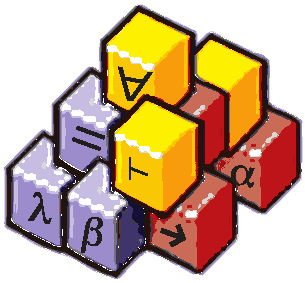
\includegraphics[height=0.75\baselineskip,keepaspectratio]{images/isabelle_logo.pdf} \texttt{\detokenize{#1}} in \texttt{\detokenize{#2}}}
\newcommand\isabellelref[2]{\begin{flushright}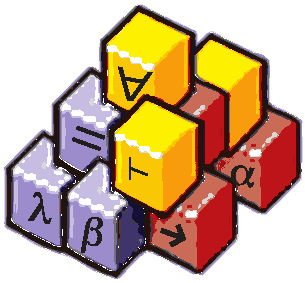
\includegraphics[height=0.75\baselineskip,keepaspectratio]{images/isabelle_logo.pdf} Also see \emph{\texttt{\detokenize{#1}}} in \emph{\texttt{\detokenize{#2}}}\end{flushright}}

\usetikzlibrary{arrows.meta}
\tikzstyle{data}=[rectangle split,rectangle split parts=2,draw,text centered]

\isabellestyle{it}
%\bibliographystyle{acm}

% Custom todo commands
\newcommand\writingtask[1]{\todo[inline]{\textbf{Writing task}: #1}}
\newcommand\missingref[1]{\todo[inline, inlinewidth=2.1cm, noinlinepar, nolist, color=gray!40, size=\tiny]{Missing reference}\todo[color=gray!40, caption={\textbf{Reference missing}: #1}]{#1}}
\newcommand\spellcheck[1]{\todo[color=green!70]{\textbf{Grammar and spellcheck}: #1}}
\newcommand\feedback[1]{\todo[color=blue!70]{\textbf{Proposed feedback}: #1}}

\begin{document}

\maketitle

\chapter*{Abstract}
\label{chapter:abstract}
Within the field of software verification, software is verified to be correct using models. However, the modelling landscape is very diverse, and multiple modelling techniques exist to model software. Model transformations can help to bridge the gap between these techniques, but often do not have a formal foundation, which is problematic for software verification. Within this work, the model transformations between models based on EMF's Ecore and GROOVE grammars are formalised. A transformation framework is introduced to create model transformations between Ecore models and GROOVE grammars while maintaining a formal foundation. This framework allows for creating significant model transformations out of smaller transformations that are more easy to proof. An application is used to show how model transformations can be built using this framework.

\tableofcontents

\section*{Introduction}

\begin{frame}{Introduction}
\begin{columns}[c]
    \begin{column}{0.05\textwidth}
    \end{column}\begin{column}{0.3\textwidth}
        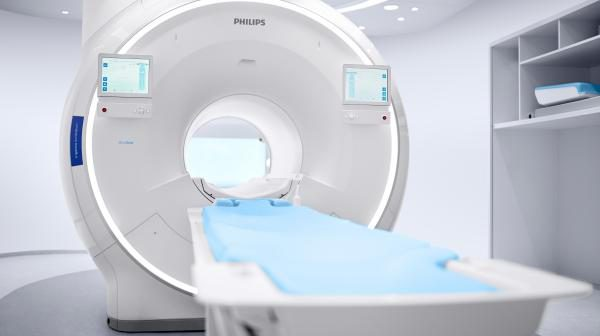
\includegraphics[width=\textwidth]{images/01_introduction/mri.jpg}
    \end{column}\begin{column}{0.3\textwidth}
        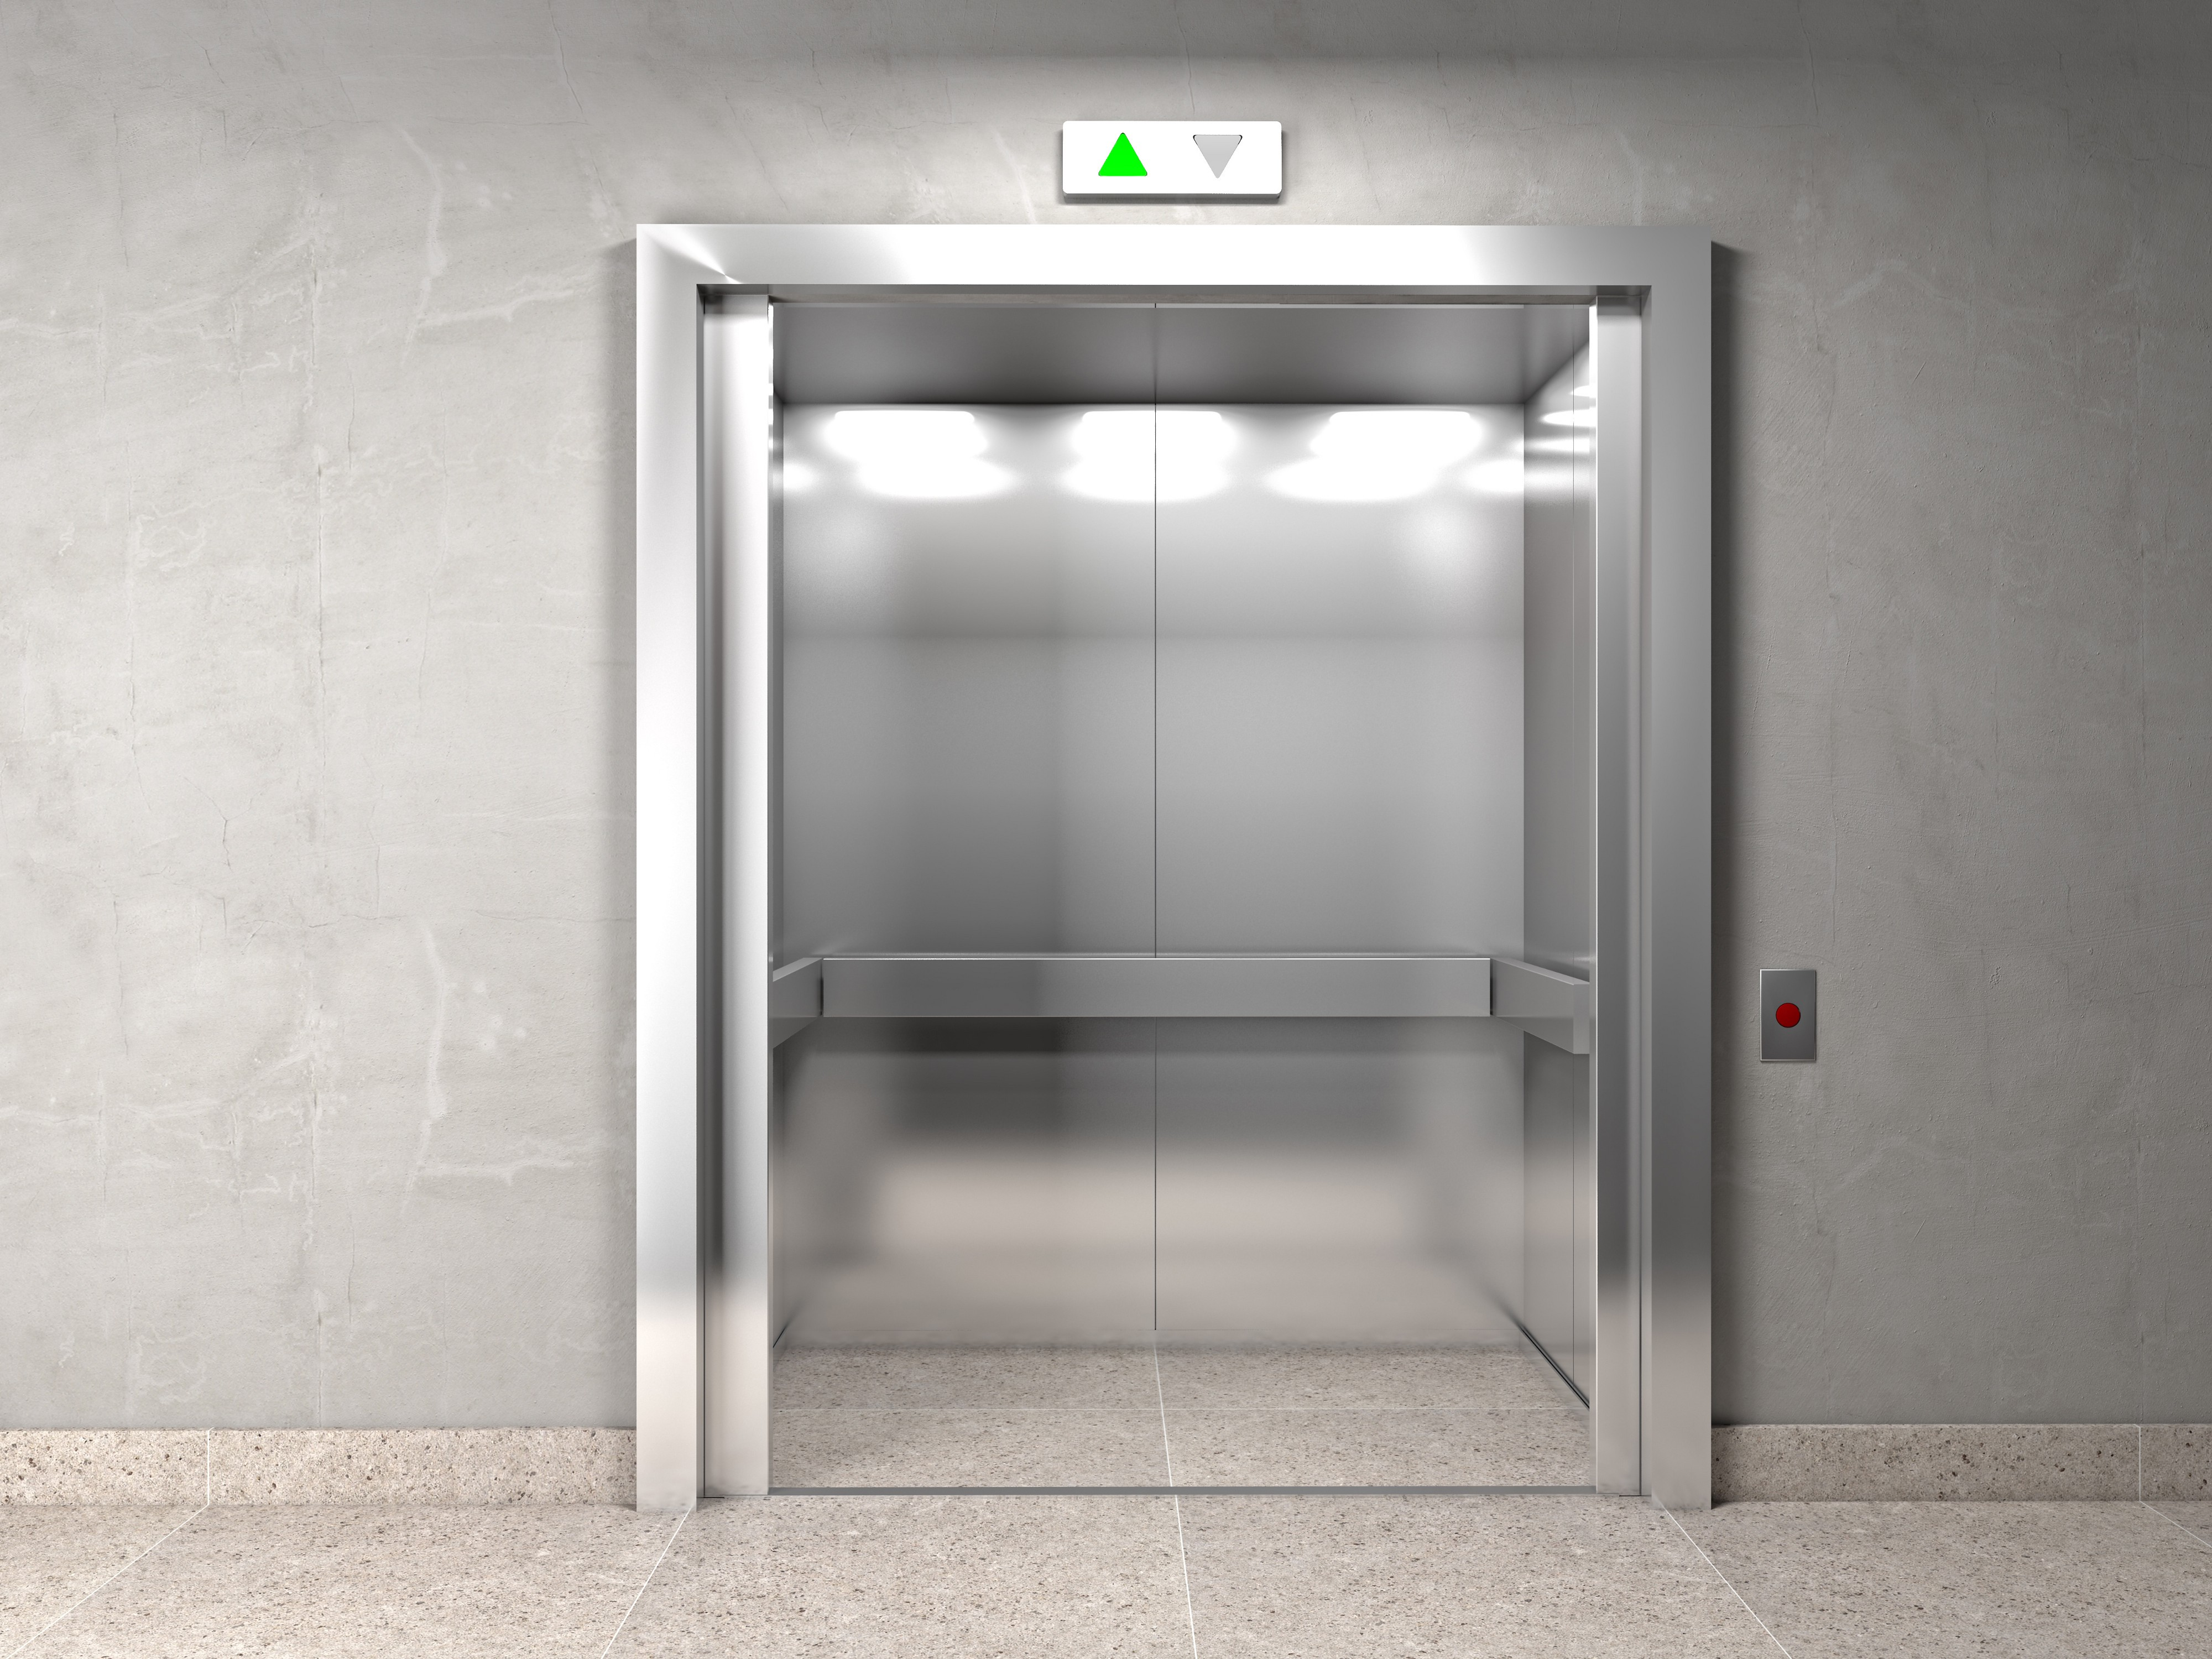
\includegraphics[width=\textwidth]{images/01_introduction/elevator.jpg}
    \end{column}\begin{column}{0.3\textwidth}
        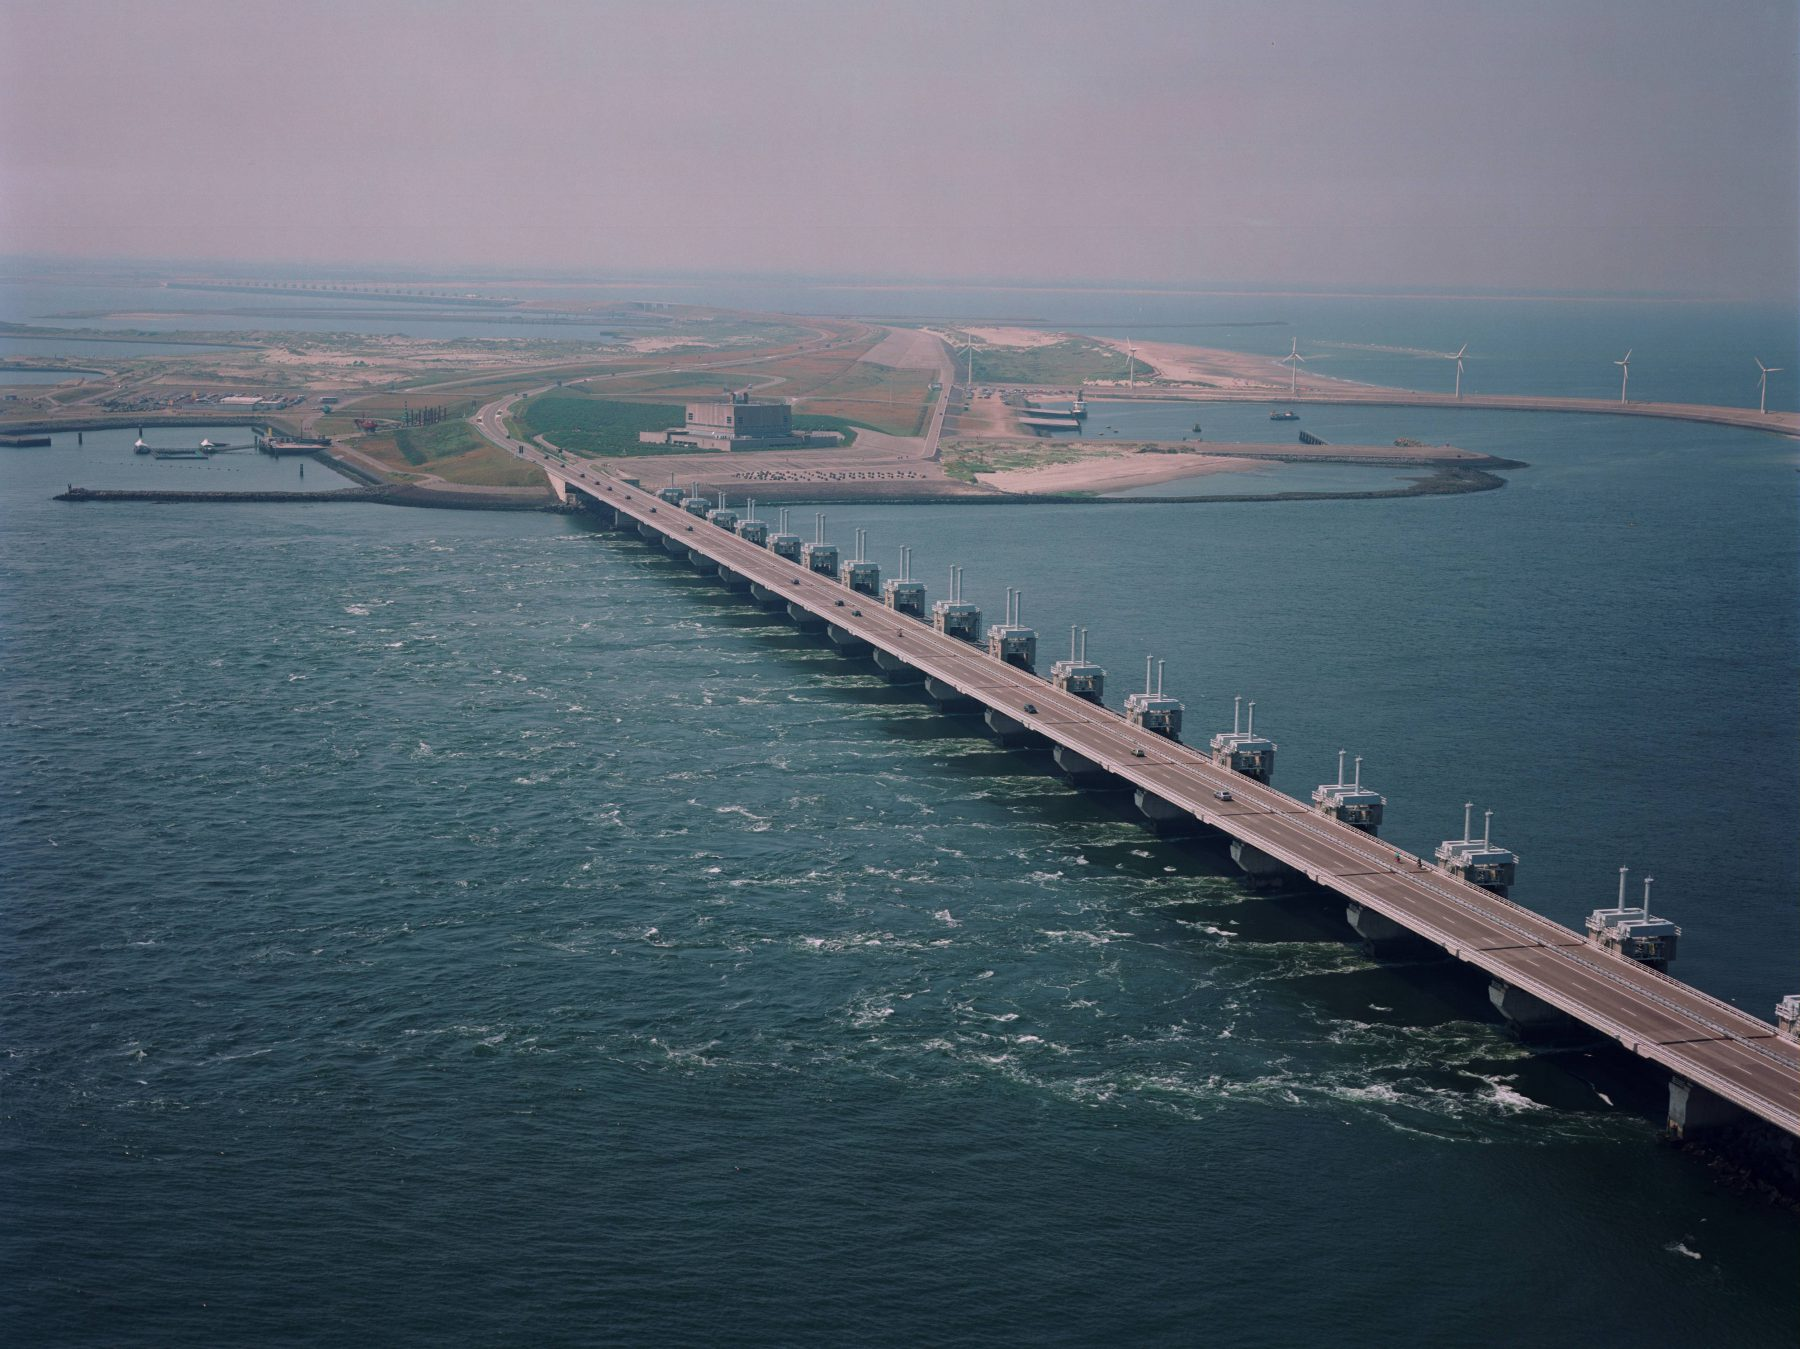
\includegraphics[width=\textwidth]{images/01_introduction/oosterscheldekering.jpg}
    \end{column}
\end{columns} 
\end{frame}

\note{
	\begin{itemize}
	    \item What have these 3 images in common?
	    \item They all make use of software systems that are crucial to be error free
	    \item How to ensure that software is error-free? Through software verification.
	\end{itemize}
}

\begin{frame}{Software verification through models}
    \centering
    \begin{tikzpicture} 
    \path
    (-3,1.5) node[inner sep=0pt](model) {% To use this figure in your LaTeX document
% import the package groove/resources/groove2tikz.sty
%
\begin{tikzpicture}[scale=0.6, every node/.style={scale=0.3}, name prefix=type-]
\node[type_node] (n0) at (0.560, -0.290) {\ml{\textbf{House}\\name: \textbf{string}}};
\node[type_node] (n1) at (0.600, -1.430) {\ml{\textbf{Room}\\number: \textbf{int}}};
\node[type_node] (n2) at (2.470, -1.435) {\ml{\textbf{Renter}}};
\node[type_node] (n3) at (2.470, -2.175) {\ml{\textit{\textbf{PaymentInterval}}}};
\node[type_node] (n4) at (1.070, -2.785) {\ml{\textbf{PaymentInterval\$MONTH}}};
\node[type_node] (n5) at (3.430, -2.785) {\ml{\textbf{PaymentInterval\$QUARTER}}};
\node[type_node] (n6) at (2.470, -0.375) {\ml{\textit{\textbf{Person}}\\age: \textbf{int}\\name: \textbf{string}}};

\path[subtype_edge](n2.north -| 2.470, -0.375) --  (n6) ;
\path[subtype_edge] (n4)  --  (n3) ;
\path[subtype_edge] (n5)  --  (n3) ;
\path[basic_edge](n2.west |- 0.600, -1.430) -- node[lab] {\ml{rents}} (n1) ;
\path[basic_edge, composite](n0.south -| 0.600, -1.430) -- node[lab] {\ml{rooms}} (n1) ;
\path[basic_edge](n2.south -| 2.470, -2.175) -- node[lab] {\ml{payment\_interval}} (n3) ;
\path[basic_edge](n1.east |- 2.470, -1.435) -- node[lab] {\ml{renter}} (n2) ;
\end{tikzpicture}
}
    (-3,-1.5) node[inner sep=0pt](checklist) {
\includegraphics[width=1.5cm]{images/01_introduction/checklist.pdf}}
    (0,0) node[inner sep=0pt](app) {
\includegraphics[width=2cm]{images/01_introduction/application.pdf}}
    (3,1.5) node[inner sep=0pt](correct) {\fontsize{40}{48} \selectfont \textcolor{ForestGreen}{\checkmark}}
    (3,-1.5) node[inner sep=0pt](incorrect) {\fontsize{40}{48} \selectfont \textcolor{red}{\ding{53}}};
    
    \path[]		
    (model) [-{Latex[width=10]}, black] edge node[above] {} (app)
    (checklist) [-{Latex[width=10]}, black] edge node[above] {} (app)
    (app) [-{Latex[width=10]}, black] edge node[above] {} (correct)
    (app) [-{Latex[width=10]}, black] edge node[above] {} (incorrect)
    ;
    \end{tikzpicture}
\end{frame}

\note{
    Explain the automated verification using a tool
	\begin{itemize}
	    \item Software model and the requirements that should be checked are given to verification software.
	    \item Verification software checks these requirements on the model.
	    \item It produces a result.
	\end{itemize}
	I will focus on obtaining the models that can be used for verification.
}

\begin{frame}{Software verification through models}
    \centering
    \begin{tikzpicture} 
    \path
    (-8,1.5) node[inner sep=0pt](fstmodel) {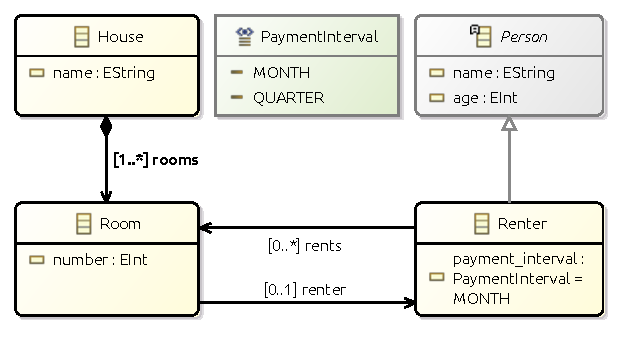
\includegraphics[width=3cm]{images/01_introduction/fstmodel.pdf}}
    (-3,1.5) node[inner sep=0pt](model) {% To use this figure in your LaTeX document
% import the package groove/resources/groove2tikz.sty
%
\begin{tikzpicture}[scale=0.6, every node/.style={scale=0.3}, name prefix=type-]
\node[type_node] (n0) at (0.560, -0.290) {\ml{\textbf{House}\\name: \textbf{string}}};
\node[type_node] (n1) at (0.600, -1.430) {\ml{\textbf{Room}\\number: \textbf{int}}};
\node[type_node] (n2) at (2.470, -1.435) {\ml{\textbf{Renter}}};
\node[type_node] (n3) at (2.470, -2.175) {\ml{\textit{\textbf{PaymentInterval}}}};
\node[type_node] (n4) at (1.070, -2.785) {\ml{\textbf{PaymentInterval\$MONTH}}};
\node[type_node] (n5) at (3.430, -2.785) {\ml{\textbf{PaymentInterval\$QUARTER}}};
\node[type_node] (n6) at (2.470, -0.375) {\ml{\textit{\textbf{Person}}\\age: \textbf{int}\\name: \textbf{string}}};

\path[subtype_edge](n2.north -| 2.470, -0.375) --  (n6) ;
\path[subtype_edge] (n4)  --  (n3) ;
\path[subtype_edge] (n5)  --  (n3) ;
\path[basic_edge](n2.west |- 0.600, -1.430) -- node[lab] {\ml{rents}} (n1) ;
\path[basic_edge, composite](n0.south -| 0.600, -1.430) -- node[lab] {\ml{rooms}} (n1) ;
\path[basic_edge](n2.south -| 2.470, -2.175) -- node[lab] {\ml{payment\_interval}} (n3) ;
\path[basic_edge](n1.east |- 2.470, -1.435) -- node[lab] {\ml{renter}} (n2) ;
\end{tikzpicture}
}
    (-3,-1.5) node[inner sep=0pt](checklist) {
\includegraphics[width=1.5cm]{images/01_introduction/checklist.pdf}}
    (0,0) node[inner sep=0pt](app) {
\includegraphics[width=2cm]{images/01_introduction/application.pdf}}
    (3,1.5) node[inner sep=0pt](correct) {\fontsize{40}{48} \selectfont \textcolor{ForestGreen}{\checkmark}}
    (3,-1.5) node[inner sep=0pt](incorrect) {\fontsize{40}{48} \selectfont \textcolor{red}{\ding{53}}};
    
    \path[]
    (fstmodel) [-{Latex[width=10]}, black] edge node[above] {Transform} (model)
    (model) [-{Latex[width=10]}, black] edge node[above] {} (app)
    (checklist) [-{Latex[width=10]}, black] edge node[above] {} (app)
    (app) [-{Latex[width=10]}, black] edge node[above] {} (correct)
    (app) [-{Latex[width=10]}, black] edge node[above] {} (incorrect)
    ;
    \end{tikzpicture}
\end{frame}

\begin{frame}{Model transformations}
    \begin{itemize}
        \item Concept from Model-driven engineering (MDE)
        \item Use a systematic approach to transform models within/between modelling languages
        \item For use in software verification, a formal foundation is required.
    \end{itemize}
\end{frame}

\note{
	\begin{itemize}
	    \item Explain that transforming models is a concept borrowed from MDE.
	    \item Explain that for verification, we want the model transformations to be proven correct, however, in most implementations this is not the case.
	\end{itemize}
}

\begin{frame}{Scope}
    \begin{itemize}
        \item Model transformations between
        \begin{itemize}
            \item EMF/Ecore
            \item GROOVE graphs
        \end{itemize}
        \item Only syntactical correctness is proven
    \end{itemize}
\end{frame}

\note{
	\begin{itemize}
	    \item Explain that my thesis focuses on solely 2 languages.
	    \item Explain that only syntactical correctness is considered within this work. Sematics are left for future work.
	\end{itemize}
}

\begin{frame}{Research questions}
    What is a suitable formalisation for composable model transformations between Ecore and GROOVE that gives rise to correct model transformations between Ecore and GROOVE?
    \pause
    \begin{itemize}
        \item What is a suitable formalisation of Ecore models and what Ecore models are valid within this formalisation? 
        \item What is a suitable formalisation of GROOVE grammars and what GROOVE grammars are valid within this formalisation? 
        \pause
        \item What is a suitable formalisation for the model transformations between Ecore and GROOVE?
        \item What model transformations are correct within the formalisation?
        \pause
        \item How can correct model transformations between Ecore and GROOVE be composed?
    \end{itemize}
\end{frame}

\note{
	\begin{itemize}
	    \item Explain the main research question. We already discussed the ingredients of the problem, so we can use that.
	    \begin{itemize}
	        \item The first two subquestions discuss the formal descriptions of EMF/Ecore and GROOVE.
	        \item The third subquestion discusses the formal description of the model transformations.
	        \item The fourth question discusses the correctness properties.
	        \item The last question is about composability, see below.
	    \end{itemize}
	    \item Leave composability on a cliffhanger. This is the only detail that was not discussed yet. In order to explain this in detail, we should first see why composability is a nice property to have, which is discussed as part of the next section.
	\end{itemize}
}

\begin{frame}{Validation}
    \begin{itemize}
        \item All proofs are checked using Isabelle, a theorem prover.
        \item Example applications show the feasibility and existance of correct model transformations.
    \end{itemize}
\end{frame}

\note{
	\begin{itemize}
	    \item The work contains a lot of mathematical formalisations and proofs, validating these is done through Isabelle, a proof assistant.
	    \item Explain that a formalisation is useless if no correct model transformations exist. An application of the proven theory shows that this is not the case.
	\end{itemize}
}

\begin{frame}{Contribution}
    Existing work on the formalisation of model transformations exists. Most important work is in the area of Triple Graph Grammars.\\
    \pause
    \vspace{0.5cm}
    What is the contribution of this thesis?
    \begin{itemize}
        \item Different approach, no conversion to graphs
        \item First formalisation of transformations between Ecore \& GROOVE specifically
    \end{itemize}
\end{frame}

\note{
	\begin{itemize}
	    \item Explain that there is earlier work on the formalisation of model transformations. Most important work is in the area of TGGs, which use graph formalisations for the modelling languages.
	    \item Explain the contribution of this work, which does not use triple graph grammars, which is an entirely different approach.
	    \item Moreover, this work focuses on Ecore/GROOVE transformations specifically, which gives rise to an formalisation that is concrete considering existing work.
	\end{itemize}
}

\begin{frame}{Contents}
\tableofcontents
\end{frame}
\chapter{Background}
\label{chapter:background}

This chapter discusses the background required to understand the different formalisations and the transformations framework introduced within this thesis. Within this chapter, EMF/Ecore is explained in more detail, as well as GROOVE. Furthermore, this chapter introduces the Isabelle proof assistant, a theorem prover which will be used to validate the proofs throughout this thesis.

\section{Eclipse Modeling Framework}
\label{sec:background:eclipse_modeling_framework}

\begin{figure}[p]
    \centering
    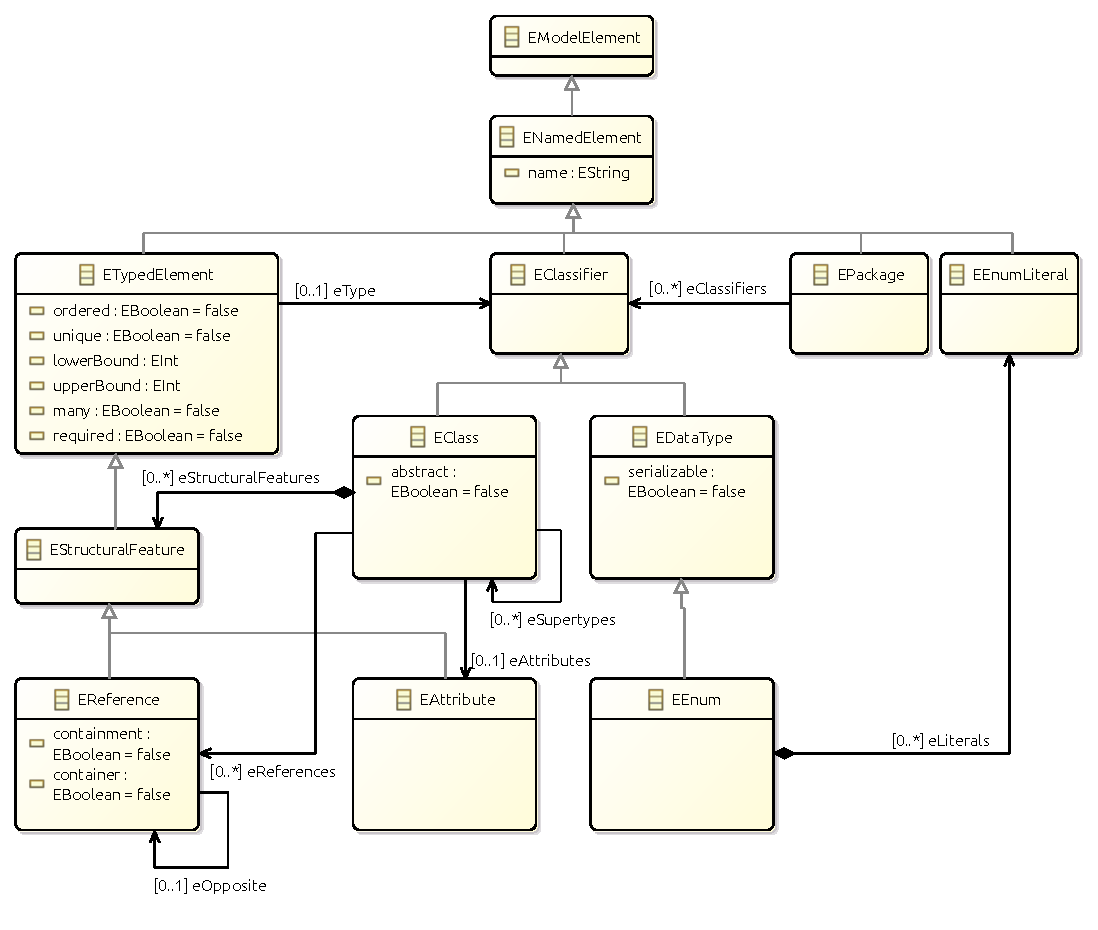
\includegraphics[width=\textwidth]{images/03_formalisations/02_ecore_formalisation/ecore.pdf}
    \caption{Simplified version of the Ecore metamodel}
    \label{fig:formalisations:ecore_formalisation:ecore}
\end{figure}

The Eclipse Modeling Framework (EMF) \cite{emf-gronback} is a modelling framework and code generation facility for building applications based on a structured model. It is quite popular in the field of Model-Driven Engineering because of its open-source nature. EMF offers support for creating, editing and translating models based on its metamodel Ecore \cite{bacvanski_graff_2005}. Models based on the Ecore metamodel are very comparable to UML class diagrams, but with properties specifically focused on software development. This focus makes models based on Ecore very suitable for object-oriented code generation as the structure of the model is already very similar to the class diagram of the corresponding application.

Because of the open-source nature of the Ecore metamodel and EMF, it has become increasingly popular for expressing domain models, creating editors for domain logic and code generation from domain models. However, EMF does not provide functionality for automated verification of its models out of the box. Different tools should be used to accomplish this task.

This thesis will focus on two levels of models based on the Ecore metamodel. The first level of models are models directly based on the Ecore metamodel, which will be called type models throughout this thesis. The second level of models are models based on a type model, and thus indirectly on the Ecore metamodel, and will be called instance models throughout this thesis. A simplified version of the Ecore metamodel \cite{emf_documentation_2015} with elements relevant to the formalisation is given in \cref{fig:formalisations:ecore_formalisation:ecore}.

\begin{figure}[H]
    \centering
    \begin{subfigure}{0.45\textwidth}
        \centering
        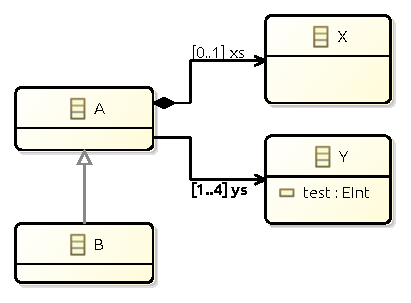
\includegraphics{images/01_introduction/type_model_intro.pdf}
        \caption{Type model}
        \label{fig:introduction:eclipse_modeling_framework:type_model}
    \end{subfigure}
    \begin{subfigure}{0.45\textwidth}
        \centering
        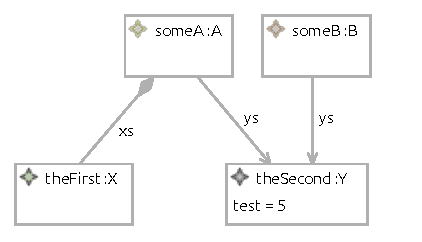
\includegraphics{images/01_introduction/instance_model_intro.pdf}
        \caption{Instance model}
        \label{fig:introduction:eclipse_modeling_framework:instance_model}
    \end{subfigure}
    \caption{Examples of different models in Ecore}
    \label{fig:introduction:eclipse_modeling_framework:ecore}
\end{figure}

\subsection{Type models}
\label{subsec:introduction:eclipse_modeling_framework:type_models}
A type model represents the first level of models based on the Ecore metamodel that will be used within this thesis. Since a type model is directly based on the Ecore metamodel, the metamodel of a type model is the Ecore metamodel. Since models based on the Ecore metamodel can best be understood as UML class diagrams, a type model can best be compared to a UML class diagram. \cref{fig:introduction:eclipse_modeling_framework:type_model} shows the visual notation of a type model in EMF's own visual notation. Familiar concepts from class diagrams can be found in this visualisation. First of all, the figure shows four class types, $\type{A}$, $\type{B}$, $\type{X}$ and $\type{Y}$. An example of inheritance of class types is shown, as class $\type{B}$ extends class $\type{A}$, so class $\type{B}$ is a subtype of class $\type{A}$. $\type{A}$ has two relations, named $\type{xs}$ and $\type{ys}$. Relation $\type{xs}$ is a relation to class $\type{X}$. Furthermore, the figure shows that $\type{xs}$ is a containment relation with a multiplicity of $0..1$. There is a second relation $\type{ys}$, which has a multiplicity of $1..4$. Finally, class $\type{Y}$ has an attribute named $\type{test}$, which represents an integer.

\subsection{Instance models}
\label{subsec:introduction:eclipse_modeling_framework:instance_models}
An instance model is the second level of models based on the Ecore metamodel that will be used in this thesis. An instance model is directly based on a type model. Therefore, the metamodel of an instance model is its corresponding type model. As a consequence, the metametamodel of an instance model is the Ecore metamodel. \cref{fig:introduction:eclipse_modeling_framework:instance_model} shows the visual notation of an instance model based on EMF's own notation, typed by the type model of \cref{fig:introduction:eclipse_modeling_framework:type_model}. The figure shows one instance of every class type. The instance of class $\type{A}$ has values for both the relations $\type{xs}$ and $\type{ys}$. The $\type{xs}$ relation references the instance of class $\type{X}$ and the $\type{ys}$ relation the instance of class $\type{Y}$. The instance of class $\type{B}$ only has a value for the relation $\type{ys}$, which references the instance of class $\type{Y}$. The instance of class $\type{Y}$ has a value set for the $\type{test}$ attribute, which is equal to integer $5$. Finally, all instances have a corresponding identifier, which is $someA$ for the instance of class $\type{A}$, $someB$ for the instance of class $\type{B}$, $theFirst$ for the instance of class $\type{X}$ and $theSecond$ for the instance of class $\type{Y}$.
\section{GROOVE}
\label{sec:background:groove}

GROOVE \cite{groove} is an open source tool which uses graphs for modelling object-oriented software and for performing verification on these graphs. GROOVE is based on graph theory and makes uses the concept of graph grammars to relate the different kind of graphs. The graphs created within a graph grammar can be further analysed using LTL and CTL properties to verify if specific properties hold on the specified graphs. When the graphs represent the design-time, compile-time, or run-time structure of a software system, the results of this analysis can be used to verify which properties hold for the software system.

GROOVE defines multiple graph types, including (but not limited to) \textit{type graphs}, \textit{instance graphs} and \textit{rule graphs}. These different graph types are used to achieve the grammar structure. Type graphs define the structure of instance graphs and rule graphs, while rule graphs describe a translation rule of an instance graph to another instance graph while maintaining the structure enforced by the type graph.

GROOVE is specially created for verification of software and uses proven techniques from logic and graph theory to verify properties on the graphs created within the tool. Although GROOVE provides excellent tools for performing verification on its graphs, there are no tools to achieve other goals, such as code generation.

This thesis will focus solely on type graphs and instance graphs. Although rule graphs might be useful in the context of model transformations and their formalisations, they are out of the scope of this thesis.

\begin{figure}[H]
    \centering
    \begin{subfigure}{0.45\textwidth}
        \centering
        % To use this figure in your LaTeX document
% import the package groove/resources/groove2tikz.sty
%
\begin{tikzpicture}[scale=\tikzscale,name prefix=type-]
\node[type_node] (n0) at (0.630, -0.720) {\ml{\textbf{A}}};
\node[type_node] (n1) at (0.630, -1.540) {\ml{\textbf{B}}};
\node[type_node] (n2) at (1.490, -0.420) {\ml{\textbf{X}}};
\node[type_node] (n3) at (1.490, -1.060) {\ml{\textbf{Y}}};

\path[basic_edge, composite] (n0)  -- node[lab] {\ml{xs}} (n2) ;
\path[basic_edge] (n0)  -- node[lab] {\ml{ys}} (n3) ;
\path[subtype_edge](n1.north -| 0.630, -0.720) --  (n0) ;
\end{tikzpicture}

        \caption{Type graph}
        \label{fig:introduction:groove:type_graph}
    \end{subfigure}
    \begin{subfigure}{0.45\textwidth}
        \centering
        % To use this figure in your LaTeX document
% import the package groove/resources/groove2tikz.sty
%
\begin{tikzpicture}[scale=\tikzscale,name prefix=instance-]
\node[basic_node] (n0) at (0.850, -0.895) {\ml{\uline{\textit{theFirst}} : \textbf{X}}};
\node[basic_node] (n1) at (2.450, -0.895) {\ml{\uline{\textit{theSecond}} : \textbf{Y}}};
\node[basic_node] (n2) at (1.700, -0.165) {\ml{\textbf{A}}};
\node[basic_node] (n3) at (2.600, -0.165) {\ml{\textbf{B}}};

\path[basic_edge] (n2)  -- node[lab] {\ml{xs}} (n0) ;
\path[basic_edge] (n3)  -- node[lab] {\ml{ys}}(n1.north -| 2.600, -0.165);
\path[basic_edge] (n2)  -- node[lab] {\ml{ys}} (n1) ;
\end{tikzpicture}

        \caption{Instance graph}
        \label{fig:introduction:groove:instance_graph}
    \end{subfigure}
    \caption{Examples of different graphs in GROOVE}
    \label{fig:introduction:groove:graphs}
\end{figure}

\subsection{Type graphs}
\label{subsec:introduction:groove:type_graphs}
As explained before, a type graph defines the structure of instance graphs and rule graphs. It is a graph type which supports concepts as inheritance, abstractness of nodes and multiplicities of edges. \cref{fig:introduction:groove:type_graph} shows the visual notation of a type graph in GROOVE its own notation. It consists of 4 nodes types, $\type{A}$, $\type{B}$, $\type{X}$ and $\type{Y}$, with 2 relations. The first relation is the $\type{xs}$ relation between $\type{A}$ and $\type{X}$ and the second relation is the $\type{ys}$ relation between $\type{A}$ and $\type{Y}$. Finally, we also see the concept of inheritance, with a subtype relation between node type $\type{B}$ and $\type{A}$.

\subsection{Instance graphs}
\label{subsec:introduction:groove:instance_graphs}
An instance graph is a graph that describes actual instances of the types defined by a type graph. The description of these instances consists of the instance itself, optional identifiers and the relation to other instances. \cref{fig:introduction:groove:instance_graph} shows the visual notation of an instance graph in GROOVE its own notation. This instance graph is based on the type graph of \cref{fig:introduction:groove:type_graph} and shows one instance of every type. The $\type{A}$-typed instance has a relation of type $\type{xs}$ to the $\type{X}$-typed instance. Furthermore, it has a relation of type $\type{ys}$ to the $\type{Y}$-typed instance. Finally, the $\type{B}$-typed instance also has a relation of type $\type{ys}$ to the same $\type{Y}$-typed instance.

It should also be noted that the $\type{X}$-typed and $\type{Y}$-typed instances have identifiers. For the $\type{X}$-typed instance, this identifier is $theFirst$, while for the $\type{Y}$-typed instance, the identifier is $theSecond$.
\section{Theorem proving using Isabelle}
\label{sec:background:theorem_proving_using_isabelle}

As mentioned before in \cref{sec:introduction:validation} all formal proofs within this paper are verified within a theorem prover, sometimes also called a proof assistant. A theorem prover is a software solution to assist with the task of proving mathematical theorems. It achieves this goal by using automated reasoning and mathematical logic to provide the user with information on the correctness of the written proof. Furthermore, a theorem prover might have tools to prove simple theorems automatically.

In this thesis, the Isabelle proof assistant is used to prove the relevant theorems. Isabelle was chosen as theorem prover for several reasons:
\begin{itemize}
    \item Isabelle stays close to mathematical definitions while still maintaining much automation in the process, which is different from other theorem provers. A comparison of theorem provers has shown that most other theorem provers which stay close to the mathematical definition do not have much automation, and vice versa \cite{wiedijk_comparing-provers}.
    \item Isabelle provides a plug-in to jEdit, a text editor, which deeply integrated Isabelle into the jEdit editor. This integration allows for interactively creating theories and checking proofs without the need to use the command-line application for this purpose.
    \item Isabelle has its own proof language Isar, which makes proofs more readable to the human reader, without giving up on automation and functionality for delivering proofs.
    \item One of the supervisors of this thesis has experience with Isabelle, meaning that there is local expertise available in case of problems.
\end{itemize}

The remaining part of this section will discuss different parts of Isabelle and its proof language Isar, to provide some background on theorem proofing in Isabelle.

\subsection{About Isabelle}
\label{subsec:background:theorem_proving_using_isabelle:about_isabelle}
Isabelle \cite{isabelle_2019} is a generic theorem prover written in \textsc{ML}. It was originally developed at the University of Cambridge and Technische Universität München, but now includes numerous contributions from institutions and individuals worldwide. It has been designed to be able to support reasoning in several object-logics, which include but are not limited to:
\begin{itemize}
    \item first-order logic, constructive and classical versions (Isabelle/FOL)
    \item higher-order logic (Isabelle/HOL)
    \item Zermelo-Fraenkel set theory (Isabelle/ZF)
\end{itemize}
Isabelle is distributed for free under a mix of open-source licenses, but the main code-base is subject to BSD-style regulations. More specifically, the binary distributions of Isabelle come with the 3-Clause BSD License \cite{bsd3clause}.

Isabelle has quite a large user base and a well-maintained community. Besides a mailing list for users, there is also a wiki \cite{isabelle_wiki} and active support on StackOverflow, when questions are tagged under `isabelle' \cite{isabelle_stack_overflow}.

The first release of Isabelle is published in 1986. Nowadays, it receives yearly releases with new updates. At the time of writing, Isabelle 2019 is the newest release, which is also the release used to prove the theorems in this thesis.

\subsection{Basics}
\label{subsec:background:theorem_proving_using_isabelle:basics}
This section will discuss some basics on Isabelle that are relevant for this thesis. The constructs mentioned here will not be discussed in much detail, as that would be a thesis on its own. The documentation provided with Isabelle does a decent job explaining all constructs in as much detail as possible.

\subsubsection{Theories}
Each document in Isabelle is a \textit{theory}, which can define a set of definitions, theorems and proofs. A theory can import other theories in order to reuse its definitions, theorems and proofs. An example of a theory is given in \cref{appendix:example_isabelle_theory}. This theory is the actual formalisation of \cref{defin:formalisations:global_definitions:multiplicity} in Isabelle used for this thesis. It will be used as an example throughout the remaining parts of this section.

\subsubsection{Datatypes}
Within an Isabelle theory, it is possible to define inductive datatypes. Inductive datatypes are the most used way to define new types in Isabelle. Famous data structures, such as lists, can be defined using datatypes.

The example provided in \cref{appendix:example_isabelle_theory} defines a new datatype for the set $\mathbb{N} \cup {\mstar}$. The definition is specified within the theory as:
\vspace{1em}\begin{isabellebody}
\isacommand{datatype}\isamarkupfalse%
\ {\isasymM}\ {\isacharequal}\ Star\ {\isacharbar}\ Nr\ nat\isanewline
\end{isabellebody}

This example defines a datatype called \isasymM{}, which can have two values: $Star$ and $Nr$. $Star$ and $Nr$ are called datatype constructors and can get arguments of different types. For example, the $Nr$ value gets an additional type, $nat$, which is Isabelle's type for representing natural numbers. On the other hand, the $Star$ constructor gets no additional arguments and is just a value for \isasymM{} on itself.

The formalisation achieved here should be straightforward. $Star$ is used to denote $\mstar$, the unbounded value, while $Nr\ nat$ is used to denote a bounded value for a multiplicity.

\subsubsection{Record types}
Another way of defining new types within Isabelle is by using record types. A record can be defined using the \textbf{record} keyword. The concept of a record is borrowed from programming languages, but it provides a way to define a named \textit{n}-tuple. Effectively, a record type is a type consisting of multiple named fields that can each have a different type. Each field of a record can be accessed using its name.

Within this thesis, records are actively used to introduce types for type models, type graphs, instance models and instance graphs. These are all named-tuples which are easiest defined using records. Sadly, the example provided in \cref{appendix:example_isabelle_theory} does not define such a record, therefore, we provide the record of an instance model (\cref{defin:formalisations:ecore_formalisation:instance_models:instance_model}) here:

\vspace{1em}\begin{isabellebody}
\isacommand{record}\isamarkupfalse%
\ {\isacharparenleft}{\isacharprime}o{\isacharcomma}\ {\isacharprime}nt{\isacharparenright}\ instance{\isacharunderscore}model\ {\isacharequal}\isanewline
\ \ Tm\ {\isacharcolon}{\isacharcolon}\ {\isachardoublequoteopen}{\isacharparenleft}{\isacharprime}nt{\isacharparenright}\ type{\isacharunderscore}model{\isachardoublequoteclose}\isanewline
\ \ Object\ {\isacharcolon}{\isacharcolon}\ {\isachardoublequoteopen}{\isacharprime}o\ set{\isachardoublequoteclose}\isanewline
\ \ ObjectClass\ {\isacharcolon}{\isacharcolon}\ {\isachardoublequoteopen}{\isacharprime}o\ {\isasymRightarrow}\ {\isacharprime}nt\ Id{\isachardoublequoteclose}\isanewline
\ \ ObjectId\ {\isacharcolon}{\isacharcolon}\ {\isachardoublequoteopen}{\isacharprime}o\ {\isasymRightarrow}\ {\isacharprime}nt{\isachardoublequoteclose}\isanewline
\ \ FieldValue\ {\isacharcolon}{\isacharcolon}\ {\isachardoublequoteopen}{\isacharparenleft}{\isacharprime}o\ {\isasymtimes}\ {\isacharparenleft}{\isacharprime}nt\ Id\ {\isasymtimes}\ {\isacharprime}nt{\isacharparenright}{\isacharparenright}\ {\isasymRightarrow}\ {\isacharparenleft}{\isacharprime}o{\isacharcomma}\ {\isacharprime}nt{\isacharparenright}\ ValueDef{\isachardoublequoteclose}\isanewline
\ \ DefaultValue\ {\isacharcolon}{\isacharcolon}\ {\isachardoublequoteopen}{\isacharprime}nt\ Id\ {\isasymRightarrow}\ {\isacharparenleft}{\isacharprime}o{\isacharcomma}\ {\isacharprime}nt{\isacharparenright}\ ValueDef{\isachardoublequoteclose}%
\end{isabellebody}

The record of an instance model directly shows the structure. It has 6 named fields, the corresponding type model and the 5 elements defined in \cref{defin:formalisations:ecore_formalisation:instance_models:instance_model}. Each of these fields has a corresponding type, corresponding to the type described within the definition of an instance model. This way, we have a direct formalisation of an instance graph in Isabelle.

\subsubsection{Type synonyms}
Isabelle can form new types out of existing types by using generic types. For example, \textit{list}s in Isabelle use this functionality. A list was created using a generic type that can be replaced with any concrete type on usage. For example `$nat\ list$' would represent a list of natural numbers, and `\isasymM$\ list$' a list of elements of datatype \isasymM.

To make it more convenient to use these types, it is possible to define these composed types as a type synonym. An example of such a type synonym is given in \cref{appendix:example_isabelle_theory}:

\vspace{1em}\begin{isabellebody}
\isacommand{type{\isacharunderscore}synonym}\isamarkupfalse%
\ multiplicity\ {\isacharequal}\ {\isachardoublequoteopen}{\isasymM}\ {\isasymtimes}\ {\isasymM}{\isachardoublequoteclose}
\end{isabellebody}

This type synonym defines the multiplicity type, effectively the formalisation of $\mathbb{M}$ from \cref{defin:formalisations:global_definitions:multiplicity}. It is a tuple of two elements of datatype \isasymM, thus a tuple $\mathbb{N} \cup \{\mstar\} \times \mathbb{N} \cup \{\mstar\}$. Using this type synonym, it is now possible to refer to the multiplicity type as `multiplicity'.

\subsubsection{Definitions and functions}
In an Isabelle theory, multiple definitions can be provided. The most basic definition can be created using the \textbf{definition} keyword. Effectively, a \textbf{definition} is simply an abbreviation, i.e. a new name for an existing construction.

An example of such a definition is the $upper$ definition in \cref{appendix:example_isabelle_theory}:
\vspace{1em}\begin{isabellebody}
\isacommand{definition}\isamarkupfalse%
\ upper\ {\isacharcolon}{\isacharcolon}\ {\isachardoublequoteopen}multiplicity\ {\isasymRightarrow}\ {\isasymM}{\isachardoublequoteclose}\ \isakeyword{where}\isanewline
\ \ {\isachardoublequoteopen}upper\ m\ {\isasymequiv}\ snd\ m{\isachardoublequoteclose}
\end{isabellebody}

As can be seen, the upper definition receives one argument $m$ of type `multiplicity', a multiplicity-tuple. It returns the upper bound of the multiplicity. In other words, it returns the second element of the tuple. This behaviour matches what the definition tells us, as $snd$ is the Isabelle function to return the second element of a tuple.

Besides the \textbf{definition} keyword, it is possible to give recursive function definitions using the \textbf{fun} and \textbf{function} keywords. An example of this is given as part of the linear order of \isasymM{} in \cref{appendix:example_isabelle_theory}:
\vspace{1em}\begin{isabellebody}
\isacommand{fun}\isamarkupfalse%
\ less{\isacharunderscore}eq{\isacharunderscore}{\isasymM}\ {\isacharcolon}{\isacharcolon}\ {\isachardoublequoteopen}{\isasymM}\ {\isasymRightarrow}\ {\isasymM}\ {\isasymRightarrow}\ bool{\isachardoublequoteclose}\ \isakeyword{where}\isanewline
{\isachardoublequoteopen}less{\isacharunderscore}eq{\isacharunderscore}{\isasymM}\ {\isacharunderscore}\ \isactrlemph \ {\isacharequal}\ True{\isachardoublequoteclose}\ {\isacharbar}\isanewline
{\isachardoublequoteopen}less{\isacharunderscore}eq{\isacharunderscore}{\isasymM}\ {\isacharparenleft}\isactrlbold a{\isacharparenright}\ {\isacharparenleft}\isactrlbold b{\isacharparenright}\ {\isacharequal}\ {\isacharparenleft}a\ {\isasymle}\ b{\isacharparenright}{\isachardoublequoteclose}\ {\isacharbar}\ \isanewline
{\isachardoublequoteopen}less{\isacharunderscore}eq{\isacharunderscore}{\isasymM}\ {\isacharunderscore}\ {\isacharunderscore}\ {\isacharequal}\ False{\isachardoublequoteclose}
\end{isabellebody}

The function defined here, `less-eq-\isasymM', defines the less than or equal to ($\leq$) relation for \isasymM. Effectively, the function describes that any value is always smaller or equal to $\mstar$ and that two numbers (two instances of $Nr$) are only less or equal when the first number is less or equal to the second number.

The same function could also have been defined using the \textbf{function} keyword, with the only difference that for the \textbf{function} keyword, a proof for termination of the function must be provided manually. Using the \textbf{fun} keyword, Isabelle will try to automatically proof termination of the function by using the specification. This automation is very powerful and works in a variety of functions (in fact, for all functions defined in this thesis, termination is proven automatically using \textbf{fun}).

\subsubsection{Abbreviations and notation}
As can be seen from the `less-eq-\isasymM' function in \cref{appendix:example_isabelle_theory}, the $Nr$ and $Star$ constructors for \isasymM{} are not used directly. Instead, numbers and a star symbol (\isactrlemph) are used to respectively represent a value of $Nr$ and the $Star$ constructor. The use of these symbols has been achieved using the \textbf{notation} keyword:
\vspace{1em}\begin{isabellebody}
\isacommand{notation}\isamarkupfalse%
\isanewline
\ \ Star\ {\isacharparenleft}{\isachardoublequoteopen}{\isacharparenleft}\isactrlemph {\isacharparenright}{\isachardoublequoteclose}\ {\isadigit{1}}{\isadigit{0}}{\isadigit{0}}{\isadigit{0}}{\isacharparenright}\ \isakeyword{and}\isanewline
\ \ Nr\ {\isacharparenleft}{\isachardoublequoteopen}{\isacharparenleft}\isactrlbold {\isacharunderscore}{\isacharparenright}{\isachardoublequoteclose}\ {\isacharbrackleft}{\isadigit{1}}{\isadigit{0}}{\isadigit{0}}{\isadigit{0}}{\isacharbrackright}\ {\isadigit{1}}{\isadigit{0}}{\isadigit{0}}{\isadigit{0}}{\isacharparenright}
\end{isabellebody}

The notation keyword allows us to introduce a new notation for many different constructs, in this case, the $Star$ and $Nr$ constructors of \isasymM. Custom notations are very powerful, as Isabelle automatically rewrites $Star$ and $Nr$ constructors back to this notation, so introducing this notation works in two ways. It can help to make theorems and proofs more readable, as can also be seen from the example in \cref{appendix:example_isabelle_theory}.

Besides the introduction of an alternative notation for existing constructs, it is also possible to introduce a new notation with the corresponding definition of what the notation means. Such a notation is achieved using the \textbf{abbreviation} keyword. It has the same properties as the \textbf{notation} keyword, but then for a newly defined definition. An example of this is given in \cref{appendix:example_isabelle_theory}:
\vspace{1em}\begin{isabellebody}
\isacommand{abbreviation}\isamarkupfalse%
\ multiplicity{\isacharunderscore}notation\ {\isacharcolon}{\isacharcolon}\ {\isachardoublequoteopen}{\isasymM}\ {\isasymRightarrow}\ {\isasymM}\ {\isasymRightarrow}\ multiplicity{\isachardoublequoteclose}\ {\isacharparenleft}{\isachardoublequoteopen}{\isacharparenleft}{\isacharunderscore}{\isacharslash}{\isachardot}{\isachardot}{\isacharunderscore}{\isacharparenright}{\isachardoublequoteclose}\ {\isacharbrackleft}{\isadigit{5}}{\isadigit{2}}{\isacharcomma}\ {\isadigit{5}}{\isadigit{2}}{\isacharbrackright}\ {\isadigit{5}}{\isadigit{1}}{\isacharparenright}\ \isakeyword{where}\isanewline
\ \ {\isachardoublequoteopen}l{\isachardot}{\isachardot}u\ {\isasymequiv}\ {\isacharparenleft}l{\isacharcomma}u{\isacharparenright}{\isachardoublequoteclose}
\end{isabellebody}

This example introduces a new notation for writing down a multiplicity tuple. It does so by writing the newly introduced notation on the left-hand side and writing the corresponding definition on the right-hand side. Although an \textbf{abbreviation} looks the same as a \textbf{definition}, they are different in the sense that \textbf{abbreviation} only introduces a notation. To Isabelle, it is syntactic sugar, as internally, the notation does not exist. It is only used when representing constructs to the user. This behaviour is different from \textbf{definition}, as definitions exist internally and are used by the proof reasoners.

It should be noted that there are shortcuts possible to introduce notations while defining a definition. An example of this is the `within{\isacharunderscore}multiplicity' definition in \cref{appendix:example_isabelle_theory}:
\vspace{1em}\begin{isabellebody}
\isacommand{definition}\isamarkupfalse%
\ within{\isacharunderscore}multiplicity\ {\isacharcolon}{\isacharcolon}\ {\isachardoublequoteopen}nat\ {\isasymRightarrow}\ multiplicity\ {\isasymRightarrow}\ bool{\isachardoublequoteclose}\ {\isacharparenleft}\isakeyword{infixl}\ {\isachardoublequoteopen}in{\isachardoublequoteclose}\ {\isadigit{5}}{\isadigit{0}}{\isacharparenright}\ \isakeyword{where}\isanewline
\ \ {\isachardoublequoteopen}n\ in\ m\ {\isasymequiv}\ lower\ m\ {\isasymle}\ \isactrlbold n\ {\isasymand}\ \isactrlbold n\ {\isasymle}\ upper\ m{\isachardoublequoteclose}\isanewline
\end{isabellebody}

This function uses the infix-left (\textbf{infixl}) construction to define an infix notation for the definition. Just like the \textbf{abbreviation} command, it is possible to use this definition on the left-hand side of the definition, for readability.

\subsubsection{Locales}
When defining new types, there is no way to constrain the values for any of its elements. For example, for the `multiplicity' type, there is no way to prevent the second value of the tuple to be 0, since the natural numbers include 0. In Isabelle, functions and types are always total, and there is no way to exclude specific values of a type.

A way to work around this is by using \textbf{locale}s. Locales are Isabelle's approach for dealing with parametric theories. With locales, it is possible to define a context in which specific assumptions hold. An example of a locale is given in \cref{appendix:example_isabelle_theory}:
\vspace{1em}\begin{isabellebody}
\isacommand{locale}\isamarkupfalse%
\ multiplicity\ {\isacharequal}\ \isakeyword{fixes}\ mult\ {\isacharcolon}{\isacharcolon}\ {\isachardoublequoteopen}multiplicity{\isachardoublequoteclose}\isanewline
\ \ \isakeyword{assumes}\ lower{\isacharunderscore}bound{\isacharunderscore}valid{\isacharbrackleft}simp{\isacharbrackright}{\isacharcolon}\ {\isachardoublequoteopen}lower\ mult\ {\isasymnoteq}\ \isactrlemph {\isachardoublequoteclose}\isanewline
\ \ \isakeyword{assumes}\ upper{\isacharunderscore}bound{\isacharunderscore}valid{\isacharcolon}\ {\isachardoublequoteopen}upper\ mult\ {\isasymnoteq}\ \isactrlbold {\isadigit{0}}{\isachardoublequoteclose}\isanewline
\ \ \isakeyword{assumes}\ properly{\isacharunderscore}bounded{\isacharbrackleft}simp{\isacharbrackright}{\isacharcolon}\ {\isachardoublequoteopen}lower\ mult\ {\isasymle}\ upper\ mult{\isachardoublequoteclose}
\end{isabellebody}

This example introduces the multiplicity locale. Within this locale, we introduce a named-construct `mult', which is a multiplicity. Then we make some assumptions which hold in the context of a multiplicity. In this case,  there are three assumptions. First of all, there are assumptions on the lower and upper bound, excluding specific (but invalid) values. The final assumption captures that the lower bound is always smaller or equal to the upper bound.

With this locale in place, it is possible to prove theorems and lemmas within the context of a multiplicity. That means that when proving theorems and lemmas within the multiplicity context, all introduced assumptions for `mult' hold:
\vspace{1em}\begin{isabellebody}
\isacommand{context}\isamarkupfalse%
\ multiplicity\isanewline
\isakeyword{begin}\isanewline
\isanewline
\isacommand{lemma}\isamarkupfalse%
\ upper{\isacharunderscore}bound{\isacharunderscore}valid{\isacharunderscore}alt{\isacharbrackleft}simp{\isacharbrackright}{\isacharcolon}\ {\isachardoublequoteopen}upper\ mult\ {\isasymge}\ \isactrlbold {\isadigit{1}}{\isachardoublequoteclose}\isanewline
%
\isadelimproof
\ \ %
\endisadelimproof
%
\isatagproof
\isacommand{using}\isamarkupfalse%
\ less{\isacharunderscore}{\isasymM}{\isachardot}elims\ not{\isacharunderscore}less\ upper{\isacharunderscore}bound{\isacharunderscore}valid\ \isacommand{by}\isamarkupfalse%
\ fastforce%
\endisatagproof
{\isafoldproof}%
%
\isadelimproof
\isanewline
%
\endisadelimproof
\isanewline
\isacommand{end}\isamarkupfalse%
\end{isabellebody}

In above example, it is possible to prove that `$upper\ mult \geq 1$ because the assumptions ensure that `$upper\ mult \not= 0$'. Since natural numbers cannot be negative, we have that `$upper\ mult \geq 1$. This theorem can only be proven within the multiplicity context, as otherwise, the assumptions do not hold, and `$upper\ mult$' might be $0$.

Within this thesis, \textbf{locale}s are mostly used to denote valid constructs, such as a valid type graph, type model, instance graph or instance model. These locales limit the respective \textbf{record} types for these constructs by assuming the validity constraints presented in their respective sections.

\subsubsection{Theorems and proofs}
Theorems (also called lemmas) are statements that can be proven correct. For this thesis, all theorems are either defined using the \textbf{theorem} or \textbf{lemma} keywords in Isabelle. A theorem can be defined to be only valid under certain assumptions or can be defined to be true without any assumptions.

An example of a simple \textbf{theorem} can be found in \cref{appendix:example_isabelle_theory}:
\vspace{1em}\begin{isabellebody}
\isacommand{theorem}\isamarkupfalse%
\ mult{\isacharunderscore}zero{\isacharunderscore}unbounded{\isacharunderscore}valid{\isacharbrackleft}simp{\isacharbrackright}{\isacharcolon}\ {\isachardoublequoteopen}n\ in\ \isactrlbold {\isadigit{0}}{\isachardot}{\isachardot}\isactrlemph {\isachardoublequoteclose}\isanewline
%
\isadelimproof
\ \ %
\endisadelimproof
%
\isatagproof
\isacommand{unfolding}\isamarkupfalse%
\ within{\isacharunderscore}multiplicity{\isacharunderscore}def\isanewline
\ \ \isacommand{by}\isamarkupfalse%
\ simp%
\endisatagproof
{\isafoldproof}%
%
\isadelimproof
\end{isabellebody}

This theorem states that for a multiplicity $0..\mstar$, any natural number is within bounds (any $n$ is in $0..\mstar$). It can easily be proven using the definition of a natural number within a multiplicity.

A proof for a theorem is written directly after the statement. It can either be a short proof using apply-scripts, or a proof within Isabelle's proof language Isar. In the example above, it is a short proof using apply-scripts. In this case, the proof is done within one step: by simplification of the definition.

Once lemmas or theorems are proven, they can be used in the proof of other lemmas and statements. Reusing them is done by referring to them manually, or by adding them to a set of lemmas and theorems that Isabelle will try by default. Adding theorems to a set of default rules is done by adding a specific keyword. For example, add $[simp]$ to add the theorem to the set of simplification rules, or add $[intro]$ or $[elim]$, to specify the theorem to be an introduction rule or elimination rule. Introduction and elimination rules will not be further specified here; more information on these can be found in the Isabelle documentation.

\subsubsection{Isar}
\textit{Isar} stands for \textit{Intelligible semi-automated reasoning}, and is an interpreted language environment for structured formal proof documents. It allows to write down mostly humanly readable proofs in Isabelle while still getting the advantage of semi-automated reasoning. Isar is built on the principle of writing down multiple steps of the proof, doing less automation, in favour of readability. As a consequence, writing Isar proofs is more work for the writer of the proof but eventually results in better humanly readable proofs that also have value without the automated reasoning of a theorem prover.

This section will not discuss the full Isar environment in detail. The Isabelle/Isar Reference Manual \cite{wenzel-isabelle_isar}, included with each copy of Isabelle, already contains a very detailed explanation of all features that Isar has to offer. Instead, we consider a small example of a proof written in Isar, picked directly from \cref{appendix:example_isabelle_theory}:
\vspace{1em}\begin{isabellebody}
\isatagproof
\isacommand{proof}\isamarkupfalse%
\isanewline
\ \ \isacommand{fix}\isamarkupfalse%
\ x\ y\ z\ {\isacharcolon}{\isacharcolon}\ {\isasymM}\isanewline
\ \ \isacommand{show}\isamarkupfalse%
\ {\isachardoublequoteopen}{\isacharparenleft}x\ {\isacharless}\ y{\isacharparenright}\ {\isacharequal}\ {\isacharparenleft}x\ {\isasymle}\ y\ {\isasymand}\ {\isasymnot}\ y\ {\isasymle}\ x{\isacharparenright}{\isachardoublequoteclose}\isanewline
\ \ \isacommand{proof}\isamarkupfalse%
\ {\isacharparenleft}induction\ x\ arbitrary{\isacharcolon}\ y{\isacharparenright}\isanewline
\ \ \ \ \isacommand{case}\isamarkupfalse%
\ Star\isanewline
\ \ \ \ \isacommand{then}\isamarkupfalse%
\ \isacommand{show}\isamarkupfalse%
\ {\isacharquery}case\ \isacommand{by}\isamarkupfalse%
\ simp{\isacharunderscore}all\isanewline
\ \ \isacommand{next}\isamarkupfalse%
\isanewline
\ \ \ \ \isacommand{case}\isamarkupfalse%
\ {\isacharparenleft}Nr\ x{\isacharparenright}\isanewline
\ \ \ \ \isacommand{then}\isamarkupfalse%
\ \isacommand{show}\isamarkupfalse%
\ {\isacharquery}case\ \isacommand{by}\isamarkupfalse%
\ {\isacharparenleft}cases\ y{\isacharparenright}\ auto\isanewline
\ \ \isacommand{qed}\isamarkupfalse%
\isanewline
\isanewline
\ \ \isacommand{show}\isamarkupfalse%
\ {\isachardoublequoteopen}x\ {\isasymle}\ x{\isachardoublequoteclose}\ \isacommand{by}\isamarkupfalse%
\ {\isacharparenleft}induction\ x{\isacharparenright}\ simp{\isacharunderscore}all\isanewline
\ \ \isacommand{then}\isamarkupfalse%
\ \isacommand{show}\isamarkupfalse%
\ {\isachardoublequoteopen}x\ {\isasymle}\ y\ {\isasymLongrightarrow}\ y\ {\isasymle}\ x\ {\isasymLongrightarrow}\ x\ {\isacharequal}\ y{\isachardoublequoteclose}\isanewline
\ \ \isacommand{proof}\isamarkupfalse%
\ {\isacharparenleft}induction\ x\ arbitrary{\isacharcolon}\ y{\isacharparenright}\isanewline
\ \ \ \ \isacommand{case}\isamarkupfalse%
\ Star\isanewline
\ \ \ \ \isacommand{then}\isamarkupfalse%
\ \isacommand{show}\isamarkupfalse%
\ {\isacharquery}case\ \isacommand{by}\isamarkupfalse%
\ {\isacharparenleft}cases\ y{\isacharparenright}\ simp{\isacharunderscore}all\isanewline
\ \ \isacommand{next}\isamarkupfalse%
\isanewline
\ \ \ \ \isacommand{case}\isamarkupfalse%
\ {\isacharparenleft}Nr\ x{\isacharparenright}\isanewline
\ \ \ \ \isacommand{then}\isamarkupfalse%
\ \isacommand{show}\isamarkupfalse%
\ {\isacharquery}case\ \isacommand{by}\isamarkupfalse%
\ {\isacharparenleft}cases\ y{\isacharparenright}\ simp{\isacharunderscore}all\isanewline
\ \ \isacommand{qed}\isamarkupfalse%
\isanewline
\isanewline
\ \ \isacommand{show}\isamarkupfalse%
\ {\isachardoublequoteopen}x\ {\isasymle}\ y\ {\isasymLongrightarrow}\ y\ {\isasymle}\ z\ {\isasymLongrightarrow}\ x\ {\isasymle}\ z{\isachardoublequoteclose}\isanewline
\ \ \isacommand{proof}\isamarkupfalse%
\ {\isacharparenleft}induction\ x\ arbitrary{\isacharcolon}\ y\ z{\isacharparenright}\isanewline
\ \ \ \ \isacommand{case}\isamarkupfalse%
\ Star\isanewline
\ \ \ \ \isacommand{then}\isamarkupfalse%
\ \isacommand{show}\isamarkupfalse%
\ {\isacharquery}case\ \isacommand{by}\isamarkupfalse%
\ {\isacharparenleft}cases\ y{\isacharparenright}\ simp{\isacharunderscore}all\isanewline
\ \ \isacommand{next}\isamarkupfalse%
\isanewline
\ \ \ \ \isacommand{case}\isamarkupfalse%
\ {\isacharparenleft}Nr\ x{\isacharparenright}\isanewline
\ \ \ \ \isacommand{then}\isamarkupfalse%
\ \isacommand{show}\isamarkupfalse%
\ {\isacharquery}case\isanewline
\ \ \ \ \isacommand{proof}\isamarkupfalse%
\ {\isacharparenleft}induction\ y\ arbitrary{\isacharcolon}\ z{\isacharparenright}\isanewline
\ \ \ \ \ \ \isacommand{case}\isamarkupfalse%
\ Star\isanewline
\ \ \ \ \ \ \isacommand{then}\isamarkupfalse%
\ \isacommand{show}\isamarkupfalse%
\ {\isacharquery}case\ \isacommand{by}\isamarkupfalse%
\ {\isacharparenleft}cases\ z{\isacharparenright}\ simp{\isacharunderscore}all\isanewline
\ \ \ \ \isacommand{next}\isamarkupfalse%
\isanewline
\ \ \ \ \ \ \isacommand{case}\isamarkupfalse%
\ {\isacharparenleft}Nr\ x{\isacharparenright}\isanewline
\ \ \ \ \ \ \isacommand{then}\isamarkupfalse%
\ \isacommand{show}\isamarkupfalse%
\ {\isacharquery}case\ \isacommand{by}\isamarkupfalse%
\ {\isacharparenleft}cases\ z{\isacharparenright}\ simp{\isacharunderscore}all\isanewline
\ \ \ \ \isacommand{qed}\isamarkupfalse%
\isanewline
\ \ \isacommand{qed}\isamarkupfalse%
\isanewline
\isanewline
\ \ \isacommand{show}\isamarkupfalse%
\ {\isachardoublequoteopen}x\ {\isasymle}\ y\ {\isasymor}\ y\ {\isasymle}\ x{\isachardoublequoteclose}\isanewline
\ \ \isacommand{proof}\isamarkupfalse%
\ {\isacharparenleft}induction\ x\ arbitrary{\isacharcolon}\ y{\isacharparenright}\isanewline
\ \ \ \ \isacommand{case}\isamarkupfalse%
\ Star\isanewline
\ \ \ \ \isacommand{then}\isamarkupfalse%
\ \isacommand{show}\isamarkupfalse%
\ {\isacharquery}case\ \isacommand{by}\isamarkupfalse%
\ simp\isanewline
\ \ \isacommand{next}\isamarkupfalse%
\isanewline
\ \ \ \ \isacommand{case}\isamarkupfalse%
\ {\isacharparenleft}Nr\ x{\isacharparenright}\isanewline
\ \ \ \ \isacommand{then}\isamarkupfalse%
\ \isacommand{show}\isamarkupfalse%
\ {\isacharquery}case\ \isacommand{by}\isamarkupfalse%
\ {\isacharparenleft}cases\ y{\isacharparenright}\ auto\isanewline
\ \ \isacommand{qed}\isamarkupfalse%
\isanewline
\isacommand{qed}\isamarkupfalse%
%
\endisatagproof
{\isafoldproof}%
%
\isadelimproof
%
\endisadelimproof
\end{isabellebody}

In this example, we see the proof that proves that type \isasymM{} is an instantiation of a linear order. In order to show that type \isasymM{} gives rise to a linear order, we have to proof multiple subgoals, which are:
\begin{itemize}
    \item Correctness of $<$: $(x < y) = (x \leq y \land \lnot y \leq x)$
    \item Reflexivity of $\leq$: $(x \leq x)$
    \item Transitivity of $\leq$: $x \leq y \land y \leq z \implies x \leq z$
    \item Correctness of the linear order: $x \leq y \lor y \leq x$
\end{itemize}
Each of these subgoals is proven separately within the Isar proof. The proof of each subgoal is defined by the \textbf{show} keyword. Important to see from the example above is that each subgoal is proven using a nested subproof. Such subproofs can be written as apply-scripts, or using a nested Isar proof, as we see in the example above.

\subsubsection{Proof tactics}
In order to deliver proofs, we make use of automated reasoning. Essential aspects of automated reasoning are the different proof tactics in Isabelle. Proof tactics can be applied to a proof goal to either solve the proof goal entirely or to somehow make the goal simpler to solve.

A vital proof tactic shown in the example above is `induction'. This tactic applies mathematical induction to the proof goal, splitting the goal into new subgoals that follow the structure of mathematical induction. 

The following proof tactics are extensively used within this thesis:
\begin{itemize}
    \item `induction' (also called `induct'): Applies mathematical induction to the proof goal. Splits the subgoal into two or more subgoals that follow the structure of mathematical induction.
    \item `cases': Applies a case distinction to the proof goal. It will split the proof goal into multiple subgoals, one for each applicable case. This proof tactic works especially well for inductive definitions and datatypes with a finite set of possible values.
    \item `intro': Splits a proof goal and introduces new subgoals based on an introduction rule. An important example of an introduction rule is $conjI$, which splits a proof goal of $A \land B$ into the two subgoals $A$ and $B$.
    \item `elim': Splits a proof goal by eliminating operations and relations and providing smaller subgoals instead of those. For example, the elimination rule $disjE$ splits a proof goal of the form $A \lor B \implies C$ into two subgoals, $A \implies C$ and $B \implies C$.
    \item `simp' (and `simp\_all'): Apply simplification to a proof goal in order to solve the problem completely. It uses simplification rules to rewrite the statement until it arrives at `True', finishing the proof.
    \item `fastforce': Solves the proof goal by using a tactic similar to brute force. It tries all possible outcomes but tries to be smart by excluding similar cases.
    \item `fast': A classical solver which solves the proof goal by structurally checking cases based on a depth-first search algorithm. Not frequently used within this thesis.
    \item `auto': A combination of `simp' and `fastforce', which can also use introduction rules and elimination rules when rewriting. In general, this proof tactic more powerful than `simp' and `fastforce'.
    \item `blast': Solves the proof goal by using a semantic tableau. Frequently used for solving logic problems.
    \item `metis': Solves the proof goal by using resolution. Frequently used for more complex logic problems that cannot be solved by `blast'.
\end{itemize}

Isabelle is not limited to the above-discussed proof tactics, but these tactics are the most important ones for this thesis. Other tactics are not used either because they apply to a different kind of problem (number arithmetic instead of logic, for example) or because they are not transparent in solving their problem. For example, the `smt' proof tactic solves a problem by using an external SMT solver. Although these proof tactics can solve many problems, it is not transparent to the reader what steps the SMT solver has taken to solve the problem, as opposed to the proof tactics described above. Therefore these tactics have been excluded.

\subsection{Archive of Formal Proofs}
Isabelle has an Archive of Formal Proofs (AFP), which is a collection of proof libraries, examples, and larger scientific developments, mechanically checked in the theorem prover Isabelle. All theories within this archive are organised in the way of a scientific journal such that they can be referred to by new theories.

\subsubsection{Graph Theory}
The Isabelle AFP submission Graph Theory \cite{noschinski-graph_theory} is used as part of this thesis. This submission to the Isabelle AFP is a formalization of directed graphs, supporting labelled multi-edges and infinite graphs. Theorems proven for these graphs include, but are not limited to, walks, cyclicity, connectedness and some properties of isomorphisms. All the theorems proven as part of this submission are discussed in \cite{bang-jensen_gutin_2010}.

Within this thesis, the submission is used as part of the GROOVE formalisation within Isabelle. Within the GROOVE formalisation, GROOVE type graphs and instance graphs are extensions of the directed graph introduced by the Graph Theory submission. This allows Isabelle to apply theorems proven for graphs within this submission to GROOVE graphs presented in the theories of this thesis.

Within this thesis, only a small selected set of theorems from the submission is used. This set mostly includes theorems related to walks and cyclicity of graphs. These theorems are used to show the acyclicity of the containment relation for instance graphs.

\chapter{Formalisations}
\label{chapter:formalisations}

As explained in \cref{sec:introduction:formalisation_of_model_transformations}, the formalisation of the model transformations depends on the formalisation of the model languages. Therefore, the formalisations of Ecore and GROOVE need to be established. In this chapter, the formalisations for Ecore and GROOVE used throughout this thesis are introduced. 

\section{Global definitions}
\label{sec:formalisations:global_definitions}

This section defines a multiplicity, which is a two tuple consisting of a lower and upper bound. In Ecore, the notion of a multiplicity is used within a field signature (\cref{defin:formalisations:ecore_formalisation:type_models:type_model}) in order to specify a limit on the allowed amount of values for a field. In GROOVE, multiplicities are used to bound the number of incoming and outgoing edges for each node type via multiplicity pairs (\cref{defin:formalisations:groove_formalisation:type_graphs:multiplicity_pair}).

\begin{defin}[Multiplicity]
\label{defin:formalisations:global_definitions:multiplicity}
A multiplicity is a two tuple consisting of a lower bound (which is any natural number) and an upper bound (which is possibly unbounded).
\begin{equation*}
\mathbb{M} \subseteq (\mathbb{N} \times \mathbb{N^+} \cup {\mstar})\ \cap \leq
\end{equation*}
The first value represents the lower bound, the second value of the tuple represents the upper bound. The set of multiplicities $\mathbb{M}$ is formally defined as
\begin{equation*}
\mathbb{M} = \{ (l, u) \mid l \in \mathbb{N} \land u \in (\mathbb{N^+} \cup {\mstar}) \land l \leq u \}
\end{equation*}
It holds that $\mstar$ is larger than each natural number, so $\forall n \in \mathbb{N}: n < \mstar$. Furthermore, the notation $l..u$ is used to denote $(l, u) \in \mathbb{M}$.

Finally, any natural number $n$ is said to be part of a multiplicity if it is within bounds, meaning:
\begin{equation*}
\forall m = l..u \in \mathbb{M}, n \in \mathbb{N} : n \in m \Leftrightarrow l \leq n \leq u
\end{equation*}
\isabellelref{multiplicity}{Ecore.Multiplicity}
\end{defin}
\section{Ecore formalisation}
\label{sec:formalisations:ecore_formalisation}

This section discusses a partial formalisation of Ecore based on the conceptual model discussed in \cite{bruintjes_bridging-groove}. The formalisation discusses both type models and instance models, as discussed in \cref{sec:background:eclipse_modeling_framework}. This formalisation has enough expressive power to capture all the elements of Ecore that are relevant for this thesis.

\subsection{Definitions}
\label{subsec:formalisations:groove_formalisation:definitions}
This section discusses some definitions specific to the GROOVE formalisation. The definitions need to be in place before the formalisations of the different GROOVE graphs are given.

GROOVE internally uses a set of labels $Lab$ for each defined grammar. These labels are used by multiple graph types of GROOVE, including (but not limited to) type graphs and instance graphs.

\begin{defin}[Labels]
\label{defin:formalisations:groove_formalisation:definitions:labels}
$Lab$ is the set of labels used by GROOVE graphs. It can be subdivided into three sets:
\begin{itemize}
    \item The set of type labels $Lab_t \subseteq Lab$
    \item The set of edge labels $Lab_e \subseteq Lab$
    \item The set of flag labels $Lab_f \subseteq Lab$
\end{itemize}

The intersection of each of the sets $Lab_t$, $Lab_f$ and $Lab_e$ has to be empty:
\begin{equation*}
    Lab_t \cap Lab_f = \emptyset \land Lab_t \cap Lab_e = \emptyset \land Lab_f \cap Lab_e = \emptyset
\end{equation*}

\isabellelref{Lab}{GROOVE.Type_Graph}
\end{defin}

The set $Lab_t$ will be used to denote the types of nodes in the graph, while the $Lab_e$ set will be used to distinguish between different edges. The $Lab_f$ set are labels for particular kind of edges which always have an identical source and target node. These are used as flags on nodes to indicate that a specific property holds for a node.

Although the intersection of each of the sets $Lab_t$, $Lab_f$ and $Lab_e$ has to be empty, the sets do not necessarily form a partition of $Lab$, as one or more of the subsets can be empty. Furthermore, $Lab$ itself can be empty if the GROOVE grammar does not define any types, flags or edge labels.

Besides $Lab$ that belongs to a grammar, GROOVE uses a set of reserved primitive type labels $Lab_{prim}$ that can never be part of the label set of a grammar.

\begin{defin}[Primitive type labels]
\label{defin:formalisations:groove_formalisation:definitions:primitive_type_labels}
GROOVE has a set of reserved primitive type labels $Lab_{prim}$:
\begin{equation*}
    Lab_{prim} = \{ \type{bool}, \type{int}, \type{real}, \type{string} \}
\end{equation*}

It should hold that $Lab \cap Lab_{prim} = \emptyset$ since the primitive type labels are reserved.
\end{defin}

The primitive type labels allow the use of primitive types as attributes and values. The label $\type{bool}$ represents the type for boolean values $\mathbb{B}$, $\type{int}$ represents the type for integer values $\mathbb{Z}$, $\type{real}$ represents the type for real numbers $\mathbb{R}$ and finally $\type{string}$ represents the type for string values $\mathbb{S}$.
\subsection{Type models}
\label{subsec:formalisations:ecore_formalisation:type_models}
This section provides the formal definition of type models, which are models that are based on the Ecore metamodel, of which a simplified version is given in \cref{fig:formalisations:ecore_formalisation:ecore}. A type model provides a set of definitions and constraints that describe a set of instance models, which may or may not be valid according to the type model. On the top level, it defines a set of \textit{classes}, \texttt{EClass}es, of which instances (\textit{objects}) may be used within the instance model. The classes contain a set of \textit{fields}, \texttt{EStructuralFeature}s, which are identified by a name which is unique within the class. Each of these \texttt{EStructuralFeature}s is typed and has a multiplicity. Class instances in the instance model may assign values to these fields (specific for that instance) which must adhere to both the type and multiplicity of the field. The type model also defines an \textit{inheritance} relation between these classes, modelled by \texttt{eSupertypes} in the Ecore metamodel, which allows classes to inherit from other classes, providing a specialisation of that class.

A type model also defines a set of \textit{enumerations}, \texttt{EEnum}s, and their values, \texttt{EEnumLiteral}s. Each enumeration defines a unique type with a fixed set of values. Furthermore, a set of \textit{constants} and their types define a symbolic typed value, which relates to a specific value in an instance model. A set of \textit{custom data types}, \texttt{EDataType}s, is also provided by the type model, which allows the representation of user-defined data types.

Finally, a set of \textit{properties} of the type model specifies the properties an instance model of this type model has to satisfy in order to be valid. These properties specify constraints on the values and structure of such an instance model.

The definition of a type model depends on the definition of various types. These types again depend on the definition of the type model. The solution to this cyclic dependency is the smallest solution to the set of equations given for the types and type model.

The suffix $Tm$ is used when the definition of something depends on any type model $Tm$, for example, $Class_{Tm}$.

\begin{defin}[Type model]
\label{defin:formalisations:ecore_formalisation:type_models:type_model}
A single type model $Tm$ is a 10-tuple, consisting of 8 sets and 2 functions, which is defined as:
\begin{equation*}
    Tm = \langle Class, Enum, UserDataType, Field, \mathrm{FieldSig}, EnumValue, Inh, Prop, Constant, \mathrm{ConstType} \rangle
\end{equation*}
with
\begin{itemize}
    \item $Class \subseteq Id$ is the set of classes (\texttt{EClass} objects) in $Tm$.
    \item $Enum \subseteq Id$ is the set of enumerations (\texttt{EEnum} objects) in $Tm$.
    \item $UserDataType \subseteq Id$ is the set of custom data types (\texttt{EDataType} objects) in $Tm$.
    \item $Field \subseteq (Class \times Name)$ is the set that maps a class to a set of field names (\texttt{EStructuralFeature} objects) in $Tm$.
    \item $\mathrm{FieldSig}: Field \Rightarrow (Type_{Tm} \times \mathbb{M})$ is the function that maps fields to their type (as defined in \cref{defin:formalisations:ecore_formalisation:type_models:types}) and multiplicity (as defined in \cref{defin:formalisations:global_definitions:multiplicity}).
    \item $EnumValue \subseteq Enum \times Name$ is the set of possible values (the \texttt{EEnumLiteral}s) for the enumerations in $Tm$.
    \item $Inh \subseteq Class \times Class$ is the inheritance relation between the classes in $Tm$.
    \item $Prop \subseteq Property_{Tm}$ is the set of properties that apply to $Tm$ (see definition \cref{defin:formalisations:ecore_formalisation:type_models:type_model_properties}).
    \item $Constant \subseteq Id$ is the set that contains all possible constants that may be used as a (symbolic) default value.
    \item $\mathrm{ConstType}: Constant \Rightarrow Type_{Tm}$ is the function that maps constants to their respective types.
\end{itemize}
where
\begin{itemize}
    \item $Class$, $DataType$ (\cref{defin:formalisations:ecore_formalisation:definitions:data_types}), $Enum$ and $UserDataType$ are pairwise disjoint.
    \item None of the elements in $Class \cup DataType \cup Enum \cup UserDataType$ may be in the namespace of another element in that set.
    \item $Inh$ is an asymmetric relation, of which the transitive closure is irreflexive.
\end{itemize}

\isabellelref{type_model}{Ecore.Type_Model}
\end{defin}

\begin{figure}[p]
    \centering
    \begin{subfigure}{\textwidth}
        \centering
        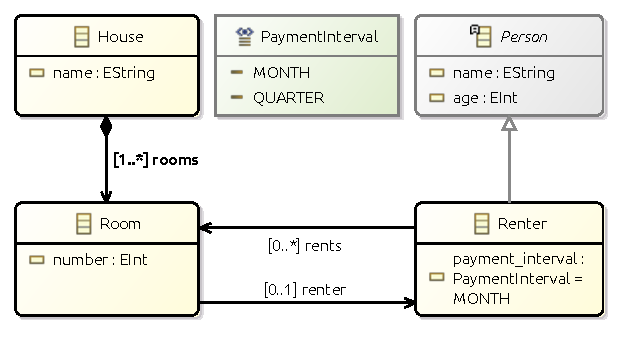
\includegraphics{images/03_formalisations/02_ecore_formalisation/type_model_example.pdf}
        \caption{Type model in Ecore notation}
    \end{subfigure}
    
    \begin{subfigure}{\textwidth}
        \centering
        \begin{align*}
            Class_{Tm} =\ & \{ 
                .\type{House}, 
                .\type{Person}, 
                .\type{Renter}, 
                .\type{Room} 
            \}\\
            Enum_{Tm} =\ & \{ 
                .\type{PaymentInterval} 
            \}\\
            UserDataType_{Tm} =\ & \emptyset\\
            Field_{Tm} =\ & \{ 
                ( .\type{House}, \type{name} ),
                ( .\type{House}, \type{rooms} ),\\&
                ( .\type{Person}, \type{age} ), 
                ( .\type{Person}, \type{name} ),\\&
                ( .\type{Renter}, \type{payment\_interval} ),
                ( .\type{Renter}, \type{rents} ),\\&
                ( .\type{Room}, \type{number} ),
                ( .\type{Room}, \type{renter} )
            \}\\
            \mathrm{FieldSig}_{Tm} =\ & \Big\{ 
                \Big( \big( .\type{House}, \type{name} \big), \big( \type{string}, 1..1 \big) \Big),
                \Big( \big( .\type{House}, \type{rooms} \big), \big( [ \type{setof},  !.\type{Room} ], 1..\mstar \big) \Big),\\&
                \Big( \big( .\type{Person}, \type{age} \big), \big( \type{integer}, 1..1 \big) \Big), 
                \Big( \big( .\type{Person}, \type{name} \big), \big( \type{string}, 1..1 \big) \Big),\\&
                \Big( \big( .\type{Renter}, \type{payment\_interval} \big), \big( .\type{PaymentInterval}, 1..1 \big) \Big),\\&
                \Big( \big( .\type{Renter}, \type{rents} \big), \big( [ \type{setof}, !.\type{Room} ], 0..\mstar \big) \Big),\\&
                \Big( \big( .\type{Room}, \type{number} \big), \big( \type{integer}, 1..1 \big) \Big),
                \Big( \big( .\type{Room}, \type{renter} \big), \big( !.\type{Renter}, 0..1 \big) \Big)
            \Big\}\\
            EnumValue_{Tm} =\ & \{ 
                ( .\type{PaymentInterval}, \type{MONTH} ),
                ( .\type{PaymentInterval}, \type{QUARTER} )
            \}\\
            Inh_{Tm} =\ & \{ 
                ( .\type{Renter}, .\type{Person} )
            \}\\
            Prop_{Tm} =\ & \{ 
                [ \type{abstract}, .\type{Person} ], \\&
                [ \type{identity}, \{( .\type{Person}, \type{age} ), ( .\type{Person}, \type{name} )\} ],
                [ \type{containment}, ( .\type{House}, \type{rooms} ) ],\\&
                [ \type{opposite}, ( .\type{Room}, \type{renter} ), ( .\type{Renter}, \type{rents} ) ], 
                [ \type{opposite}, ( .\type{Renter}, \type{rents} ), ( .\type{Room}, \type{renter} ) ],\\&
                [ \type{defaultValue}, ( .\type{Renter}, \type{payment\_interval} ), .\type{Constant}.\type{PaymentInterval}.\type{Month} ]
            \}\\
            Constant_{Tm} =\ & \{ 
                .\type{Constant}.\type{PaymentInterval}.\type{Month}
            \}\\
            \mathrm{ConstType}_{Tm} =\ & \{ 
                ( .\type{Constant}.\type{PaymentInterval}.\type{Month}, .\type{PaymentInterval} )
            \}
        \end{align*}
        \caption{Formal definition of the type model}
    \end{subfigure}
    \caption{Example of a type model corresponding with \cref{defin:formalisations:ecore_formalisation:type_models:type_model}}
    \label{fig:formalisations:ecore_formalisation:type_models:type_model_example}
\end{figure}

An example type model is given in \cref{fig:formalisations:ecore_formalisation:type_models:type_model_example}. It shows 4 classes ($\type{House}$, $\type{Person}$, $\type{Renter}$ and $\type{Room}$) and a single enumeration ($\type{PaymentInterval}$). The $\type{Person}$ class has 2 fields, $\type{age}$ and $\type{name}$. The $\type{Renter}$ class has a field $\type{payment\_interval}$ which makes use of the $\type{PaymentInterval}$ enumeration. It also has a field $\type{rents}$ which defines a relation between $\type{Room}$ and $\type{Renter}$. The $\type{House}$ class has also 2 fields, a field $\type{name}$ and a field $\type{rooms}$ which is a containment relation between $\type{House}$ and $\type{Room}$. Moreover, we have the $\type{Room}$ class itself, which has 2 fields. One is called $\type{number}$ and the other one is called $\type{renter}$, which is the opposite relation between $\type{Room}$ and $\type{Renter}$. Finally, we see that $\type{Renter}$ inherits from $\type{Person}$.

The fields in a type model are always associated with a specific type, which defines the set of possible values that may be assigned in an instance model. The possible types are defined by the set of data types, classes, enumerations and user-defined data types. The set of types also consists of various aggregations of these types, namely containers. Containers provide types for multiple values of the same type, but of which the values may differ in number and order.

\begin{defin}[Types]
\label{defin:formalisations:ecore_formalisation:type_models:types}
Given any type model $Tm$, the set of types is defined as
\begin{equation*}
Type_{Tm} = DataType \cup ClassType_{Tm} \cup Enum_{Tm} \cup UserDataType_{Tm} \cup Container_{Tm}
\end{equation*}

The $ClassType_{Tm}$ set defines both a set of nullable and proper classes. Nullable classes are classes for which the $\type{nil}$ (see \cref{defin:formalisations:ecore_formalisation:definitions:nil}) value is valid, and proper classes are those classes for which the $\type{nil}$ value is not valid (hence both sets of classes are disjoint). 

The $ClassType_{Tm}$ set is defined as
\begin{equation*}
ClassType_{Tm} = \{ \type{nullable}, \type{proper} \} \times Class_{Tm}
\end{equation*}

A container is a type that may contain multiple values in an instance. Containers define the type of values they contain, and the multiplicity of the container. They are defined by 
\begin{equation*}
Container_{Tm} = \{ \type{bagof}, \type{setof}, \type{seqof}, \type{ordof} \} \times Type_{Tm}
\end{equation*}
For the interpretation of the values in $\{ \type{bagof}, \type{setof}, \type{seqof}, \type{ordof} \}$, see \cref{defin:formalisations:ecore_formalisation:instance_models:values}.

The set of types is recursively defined as the smallest solution of the equations for $Type_{Tm}$ and $Container_{Tm}$.

Tuples within $Type_{Tm}$ are written using square brackets, e.g. $[\type{bagof}, \type{int} ]$ or $[ \type{nullable}, C ]$. Furthermore, given a $C \in Class_{Tm}$, $?C$ is a short notation for the $\type{nullable}$ variant of $C$, $[ \type{nullable}, C ]$. In the same fashion, $!C$ is the short notation for the $\type{proper}$ variant of $C$, $[ \type{proper}, C ]$.

Finally, we define the function $\mathrm{uncontainer}\!: Container_{Tm} \Rightarrow Type_{Tm}$ which returns the type contained by a container.

\isabellelref{Type}{Ecore.Type_Model}
\end{defin}

In the example in \cref{fig:formalisations:ecore_formalisation:type_models:type_model_example}, the various fields make use of different types. The fields depicted as a relation between two classes are actually of a type based on the $Class_{Tm}$ set. For example, the $\type{rooms}$ field of class $\type{House}$ is typed by the $\type{Room}$ class. In this case, we assume that each $\type{Room}$ in a $\type{House}$ is unique. Thus the relationship is best typed by a $\type{setof}$ container. For a $\type{setof}$ container, the order does not matter, and each value should be unique. We also see the example of the usage of an enumeration, the $\type{payment\_interval}$ field on $\type{Renter}$ uses the $\type{PaymentInterval}$ enumeration. Finally, the $\type{Person}$ class shows two fields that are typed by some of the data types available, integer and string for the age and name fields respectively.

\begin{defin}[Field]
\label{defin:formalisations:ecore_formalisation:type_models:field}
Given any type model $Tm$, the $Field_{Tm}$ relation defines a binary relation between classes and fields.
In order to retrieve the set of fields for a given class (and the fields inherited from superclasses), the following function is defined:
\begin{equation*}
   \mathrm{fields}\!: Class_{Tm} \Rightarrow \mathcal{P}(Field_{Tm})
\end{equation*}
such that
\begin{equation*}
\mathrm{fields}_{Tm}(c) = \{f \in Field_{Tm} \mid f = ( c', n ) \land c \sqsubseteq_{Tm} c'\}
\end{equation*}

Given any type model $Tm$, the $\mathrm{FieldSig}_{Tm}$ function defines a mapping between fields and their signatures. The following functions are defined to retrieve various components of a field signature:
\begin{itemize}
    \item $\mathrm{class}\!: Field_{Tm} \Rightarrow Class_{Tm}$
    \item $\mathrm{type}\!: Field_{Tm} \Rightarrow Type_{Tm}$
    \item $\mathrm{lower}\!: Field_{Tm} \Rightarrow \mathbb{N}$
    \item $\mathrm{upper}\!: Field_{Tm} \Rightarrow \mathbb{N}^+ \cup {\mstar}$
\end{itemize}
These functions are defined as follows:
\begin{itemize}
    \item $\mathrm{class}_{Tm}(f) = class \quad \mathrm{iff} \quad f = ( class, name)$
    \item $\mathrm{type}_{Tm}(f) = type \quad \mathrm{iff} \quad \mathrm{FieldSig}_{Tm}(f) = ( type, ( lower, upper ) )$
    \item $\mathrm{lower}_{Tm}(f) = lower \quad \mathrm{iff} \quad \mathrm{FieldSig}_{Tm}(f) = ( type, ( lower, upper ) )$
    \item $\mathrm{upper}_{Tm}(f) = upper \quad \mathrm{iff} \quad \mathrm{FieldSig}_{Tm}(f) = ( type, ( lower, upper ) )$
\end{itemize}

Fields can be separated into relation and attribute sets, where attributes reference (containers of) data types, user data types and enumerations, and relations reference all other types. The sets are defined by
\begin{align*}
    Attr_{Tm} =&\, \{f \in Field_{Tm} \mid type(f) \in (DataType \cup Enum_{Tm} \cup UserDataType_{Tm})\,\vee\\&\quad type(f) \in \{ \type{setof}, \type{bagof}, \type{ordof}, \type{seqof} \} \times Attr_{Tm}\}\\
    Rel_{Tm} =&\, Field_{Tm} \setminus Attr_{Tm}
\end{align*}
The set of attributes is recursively defined as the smallest solution of the given set of equations for $DataType$, $Enum_{Tm}$, $UserDataType_{Tm}$ and $Attr_{Tm}$

\isabellelref{fields}{Ecore.Type_Model}
\end{defin}

Taking for example the field $\type{rents}$ from the $\type{Renter}$ class in the type model example in \cref{fig:formalisations:ecore_formalisation:type_models:type_model_example}, the following properties can be identified: The type refers to $\type{Room}$, which is an element of the $Class_{Tm}$ set. The
lower and upper values are $0$ and $\mstar$ respectively (which means a $\type{Renter}$ can rent an arbitrary number of rooms). Furthermore, the $\type{rents}$ field is an element of the $Rel_{Tm}$ set (it is a class container type) and part of the $fields_{Tm}(\type{Renter})$ set, which is $\{ \type{payment\_interval}, \type{rents} \}$.

The various types have an underlying subtype relation, which generalises inheritance. A subtype defines a specialisation of a supertype. Because of that, all values valid for the subtype are also valid for the supertype (see \cref{defin:formalisations:ecore_formalisation:instance_models:valid_type_values} for details).

\begin{defin}[Subtype relation]
\label{defin:formalisations:ecore_formalisation:type_models:subtype_relation}
Given any type model $Tm$, $\sqsubseteq_{Tm}\, \subseteq Type_{Tm} \times Type_{Tm}$ defines the subtype relation. It is a reflexive partial order relation, for which the following rules
can be defined (with $t_1, t_2, t_3 \in Type_{Tm}$ and $c_1, c_2 \in Class_{Tm}$):

Transitivity:
\begin{mathpar}
    \inferrule{t_1 \sqsubseteq_{Tm} t_2 \\ t_2 \sqsubseteq_{Tm} t_3}{t_1 \sqsubseteq_{Tm} t_3}
\end{mathpar}

Reflexivity:
\begin{mathpar}
    \inferrule{\ }{t_1 \sqsubseteq_{Tm} t_1}
\end{mathpar}

Generalization of inheritance:
\begin{mathpar}
    \inferrule{(c_1, c_2) \in Inh_{Tm}}{?c_1 \sqsubseteq_{Tm}\: ?c_2}
    \and
    \inferrule{(c_1, c_2) \in Inh_{Tm}}{!c_1 \sqsubseteq_{Tm}\: !c_2}
\end{mathpar}

Nullable/Proper classes:
\begin{mathpar}
    \inferrule{\ }{!c_1 \sqsubseteq_{Tm}\: ?c_1}
\end{mathpar}

\isabellelref{subtype}{Ecore.Type_Model}
\end{defin}

Thus, in the example, $[ \type{nullable}, \type{Renter} ] \sqsubseteq_{Tm} [ \type{nullable}, \type{Person} ]$ (since $(\type{Student}, \type{Person}) \in Inh_{Tm}$). Furthermore, it also holds that $[ \type{proper}, \type{Renter} ] \sqsubseteq_{Tm} [ \type{nullable}, \type{Renter} ]$, as a proper class is a subtype of a nullable class.

A type model may specify a set of properties, $Prop$, which an instance model has to satisfy in order to be valid. The following properties are defined:
\begin{itemize}
\item The $\type{abstract}$ property. This property, specified for a specific class in the type model, forbids the instantiation of that class in any instance model. As such, it is satisfied when no object exists in an instance model which is an instance of that class. Please note that this only holds for instances of that exact class. Subtyping may be allowed (under the condition that those classes are not $\type{abstract}$).

\item The $\type{containment}$ property. This property, specified for a relation, states that a single source object contains all objects that are the target of this relation. Objects are contained by at most one other object, and containment cycles are not allowed. When an object with contained objects is removed from an instance model, all contained objects are removed as well. The constraint is satisfied when an object is the target of no more than one containment relation, and there exists no cycle between containment relations.

\item The $\type{defaultValue}$ property. This property specifies a default value for a field which has not been assigned a value in an instance model. It specifies a constant for a field, which represents a value in an instance model. It is always satisfied and influences the behaviour of possible model transformations.

\item The $\type{identity}$ property. This property is specified for a class and a set of attributes. It is used to specify that the values for the set of attributes uniquely identify an object on instance model level. As such, it is satisfied when no two objects are both an instance of the class and have pairwise the same value for all the attributes.

\item The $\type{keyset}$ property. This property is specified for a set of attributes of a class and a relation towards that class. It ensures that each instance of that class within the given relation is uniquely identified by the values of the set of attributes. It is satisfied that two objects must be the same object if they are the target of the given relation, and they have pairwise-identical values for their attributes.

\item The $\type{opposite}$ property. This property specifies that two relations are the opposite of each other, which means that for each instance of the first relation, an instance of the second relation exists with a switched target and source. The property is satisfied when for each pair of objects, for each relation that exists between these objects, a reverse relation exists if both these relations are opposite.

\item The $\type{readonly}$ property. This property, specified for a field in the type model, forbids the assignment of a new value to that field in any instance model. This property only affects the possible transformations of an instance model and is always satisfied for any specific instance model.
\end{itemize}

\begin{defin}[Type model properties]
\label{defin:formalisations:ecore_formalisation:type_models:type_model_properties}
For a type model $Tm$ a set of properties $Property_{Tm}$ is defined which contains all the possible properties. This set is defined as 

\begin{align*}
    Property_{Tm} =\ &
    \{[ \type{abstract}, c ] \mid c \in Class_{Tm} \}\ \cup \\&
    \{[ \type{containment}, r ] \mid r \in Rel_{Tm} \}\ \cup \\&
    \{[ \type{defaultValue}, f, v ] \mid f \subseteq Field_{Tm} \land v \in Constant_{Tm} \}\ \cup \\&
    \{[ \type{identity}, c, A ] \mid c \in Class_{Tm} \land A \subseteq Attr_{Tm} \}\ \cup \\&
    \{[ \type{keyset}, r, A ] \mid r \in Rel_{Tm} \land A \subseteq Attr_{Tm} \}\ \cup \\&
    \{[ \type{opposite}, r, r' ] \mid r, r' \subseteq Rel_{Tm} \land r \not= r'\}\ \cup \\&
    \{[ \type{readonly}, f ] \mid f \in Field_{Tm} \}
\end{align*}

where
\begin{itemize}
    \item $[ \type{defaultValue}, f, v ]$ is defined such that $\mathrm{ConstType}_{Tm}(v) \sqsubseteq_{Tm} \mathrm{type}_{Tm}(f)$.
    \item $[ \type{keyset}, r, A ]$ is defined such that $\mathrm{type}_{Tm}(r) \in (\{ \type{setof}, \type{ordof} \} \times ClassType_{Tm})$ with $\mathrm{type}_{Tm}(r) = [\type{setof}, c] \lor \mathrm{type}_{Tm}(r) = [ \type{ordof}, c ]$. Then also have that $\forall ( ac, an ) \in A\!:\: !c\sqsubseteq_{Tm}\,!ac$.
    \item $[ \type{opposite}, r, r' ]$ is defined such that when $r = ( c1, n1 ), r' = ( c2, n2 )$, then it should hold that $!c1 \sqsubseteq_{Tm} \mathrm{uncontainer}(\mathrm{type}_{Tm}(r'))$, $!c2 \sqsubseteq_{Tm} \mathrm{uncontainer}(\mathrm{type}_{Tm}(r))$, $\mathrm{type}_{Tm}(r) \not\in \{ \type{bagof}, \type{seqof} \} \times Type_{Tm}$ and finally $type_{Tm}(r') \not\in \{ \type{bagof}, \type{seqof} \} \times Type_{Tm}$ (containers must have unique values).
\end{itemize}

\isabellelref{Property}{Ecore.Type_Model}
\end{defin}

The example in \cref{fig:formalisations:ecore_formalisation:type_models:type_model_example} also shows a few properties:
\begin{itemize}
    \item The $\type{Person}$ class is declared abstract (indicated by the grey looking class layout and italic name)
    \item The $\type{age}$ and $\type{name}$ fields of a $\type{Person}$ are its identity (as indicated by the formal definition). Although it is highly unlikely that these details would be unique in the real world, they must be in our instance models.
    \item The $\type{rooms}$ relation of $\type{House}$ is a containment relation (shown by the filled diamond at the $\type{House}$ end of the containment relation).
    \item The $\type{rents}$ and $\type{renter}$ relations are opposites (as indicated by the formal definition).
    \item The $\type{payment\_interval}$ field has a default value $\type{MONTH}$ (as indicated with the field definition in the model).
\end{itemize}

With the given definitions, it is possible to define an inconsistent type model. Such a type model is correct according to the given definitions but does not specify any valid instance model using the definitions in \cref{subsec:formalisations:ecore_formalisation:instance_models}. Therefore, a definition is given for a consistent type model. A consistent type model enforces some constraints on multiplicities and properties within the type model to ensure the satisfiability of the definitions in \cref{subsec:formalisations:ecore_formalisation:instance_models}. Without these constraints, one or more of these definitions can never be satisfied at all. Please note that these constraints merely support the satisfiability of these definitions, it does not guarantee the existence of any meaningful instance model, as it might still be possible to define a `consistent' type model with conflicting multiplicities or properties.

\begin{table}[t]
    \centering
    \rowcolors{2}{gray!25}{white}
    \begin{tabular}{l|l}
        \rowcolor{gray!50}
        $Type_{Tm}$ & Multiplicity\\
        $\{ \type{proper} \} \times Class_{Tm}$ & $1..1$\\
        $\{ \type{nullable} \} \times Class_{Tm}$ & $0..1$\\
        $Container_{Tm}$ & $x..y \: (0 \leq x \leq y \land 1 \leq y)$\\
        $DataType$ & $1..1$\\
        $Enum_{Tm}$ & $1..1$\\
        $UserDataType_{Tm}$ & $1..1$
    \end{tabular}
    \caption{The allowed multiplicities for each type}
    \label{tab:formalisations:ecore_formalisation:type_models:possible_multiplicities}
\end{table}

\begin{defin}[Type model consistency]
\label{defin:formalisations:ecore_formalisation:type_models:type_model_consistency}
The multiplicities of the fields in $Field_{Tm}$ are consistent if it holds that:
\begin{align*}
    \mathrm{type}_{Tm}(f) \in DataType \cup Enum_{Tm} \cup UserDataType_{Tm} \cup (\type{proper} \times Class_{Tm}) \implies & \mathrm{lower}_{Tm}(f) = 1 \\
    \mathrm{type}_{Tm}(f) \in (\type{nullable} \times Class_{Tm}) \implies & \mathrm{lower}_{Tm}(f) = 0
\end{align*}
and
\begin{align*}
    \mathrm{type}_{Tm}(f) \not\in Container_{Tm} \implies & \mathrm{upper}_{Tm}(f) = 1
\end{align*}
as indicated by \cref{tab:formalisations:ecore_formalisation:type_models:possible_multiplicities}.

The properties in $Prop_{Tm}$ are consistent if the following holds:
\begin{itemize}
    \item $[ \type{containment}, r ] \in Prop_{Tm} \land [ \type{opposite}, r, r' ] \in Prop_{Tm} \Longrightarrow upper_{Tm}(r') = 1$ (opposite of containment relation must have upper bound of 1).
    \item $[ \type{defaultValue}, f, v ] \in Prop_{Tm} \land [ \type{defaultValue}, f, v' ] \in Prop_{Tm} \Longrightarrow v = v'$ (unique for f).
    \item $[ \type{identity}, c_1, A_1 ] \in Prop_{Tm} \land [ \type{identity}, c_2, A_2 ] \in Prop_{Tm}\: \land\: !c_1 \sqsubseteq_{Tm}\, !c_2 \Longrightarrow A_1 \subseteq A_2$ (classes may only have identities with attributes that are a subset of attributes part of the superclass' identity).
    \item $[ \type{keyset}, r, A ] \in Prop_{Tm} \land [ \type{keyset}, r, A' ] \in Prop_{Tm} \Longrightarrow A = A'$ (unique for $r$).
    \item $[ \type{opposite}, r, r' ] \in Prop_{Tm} \land [ \type{opposite}, r, r'' ] \in Prop_{Tm} \Longrightarrow r' = r''$ (unique for r).
    \item $[ \type{opposite}, r, r' ] \in Prop_{Tm} \Longleftrightarrow [ \type{opposite}, r', r ] \in Prop_{Tm}$ (symmetry).
\end{itemize}

Then a type model $Tm$ is consistent if and only if
\begin{itemize}
\item The multiplicities of all fields in $Field_{Tm}$ are consistent.
\item All properties in $Prop_{Tm}$ are consistent.
\end{itemize}

\isabellelref{type_model}{Ecore.Type_Model}
\end{defin}
\subsection{Instance models}
\label{subsec:formalisations:ecore_formalisation:instance_models}
An instance model represents an instance of a type model. In other words, the metamodel of an instance model is its type model. Because of our definitions of type models, this means that the metametamodel of an instance model is the Ecore metamodel.

An instance model consists of a set of objects, which have a corresponding class they instantiate and an optional identifier. All objects are an instance of a specific class and are therefore typed by that class and its superclasses. Furthermore, an instance model also specifies the values for each field of an object. Its type determines the fields present for each object. Finally, the instance model specifies a set of default values, which assigns a value to each of the named constants from the type model ($Constant_{Tm}$), allowing to assign default values to fields.

As with the type model and type definitions, there is a cyclic dependency between instance models and values. In the same manner, the solution is set to be the smallest solution to the set of equations for the instance model and values.

The suffix $Im$ is used when the definition of something depends on any instance model $Im$, which itself depends on the definition of any type model $Tm$.

\begin{defin}[Instance model]
\label{defin:formalisations:ecore_formalisation:instance_models:instance_model}
For a type model $Tm$,
\begin{equation*}
    Tm = \langle Class, Enum, UserDataType, Field, \mathrm{FieldSig}, EnumValue, Inh, Prop, Constant, \mathrm{ConstType} \rangle
\end{equation*}
a single instance model $Im$ is defined as
\begin{equation*}
    Im = \langle Object, \mathrm{ObjectClass}, \mathrm{ObjectId}, \mathrm{FieldValue}, \mathrm{DefaultValue} \rangle
\end{equation*}
with
\begin{itemize}
    \item $Object$ is the set of objects (class instances) in $Im$.
    \item $\mathrm{ObjectClass}: Object \Rightarrow Class_{Tm}$ is the function that maps each object in $Im$ to a class.
    \item $\mathrm{ObjectId}: Object \Rightarrow Name$ is the injective partial function that maps each object in $Im$ to an identifier.
    \item $\mathrm{FieldValue}: (Object \times Field_{Tm}) \Rightarrow Value_{Im}$ is the partial function between each $Field_{Tm}$ of an $Object_{Im}$ and a $Value_{Im}$ (see \cref{defin:formalisations:ecore_formalisation:instance_models:values}).
    \item $\mathrm{DefaultValue}: Constant_{Tm} \Rightarrow Value_{Im}$ is the function that assigns a value to each constant in the corresponding type model $Tm$.
\end{itemize}
where
\begin{itemize}
    \item $\forall ( o, n ), ( o', n' ) \in ObjectId: n = n' \Longrightarrow o = o'$.
    \item $\forall o \in Object, f \in Field_{Tm}: ( o, f ) \in \mathrm{dom}\ FieldValue \Longleftrightarrow ObjectClass(o) \sqsubseteq_{Tm} \mathrm{class}(f)$.
\end{itemize}

\isabellelref{instance_model}{Ecore.Instance_Model}
\end{defin}

Please note that $\mathrm{ObjectId}$ is injective because each object must have a unique identifier. It is partial because an object does not necessarily need an identifier: The internal object identifiers (the elements of the set $Object$) are already unique. The $\mathrm{ObjectId}$ function is for adding an explicit identifier that is not generated internally.

The $\mathrm{FieldValue}$ function maps a combination of an object and field to a value. Please note that the function is partial because not every combination of object and field is valid. The domain of this function is therefore made explicit by the constraints of the definition. Please note that this function is not injective: Values can be shared across objects and do not have to be unique.

An important function is the $\mathrm{DefaultValue}$ function, which is defined on an instance model rather than a type model. This definition has been chosen to accommodate for default values that reference another object. In order to reference another object, the possible object references need to be known. These object references are only known on the instance level, as the type level does not define any objects.

\begin{figure}[p]
    \centering
    \begin{subfigure}{\textwidth}
        \centering
        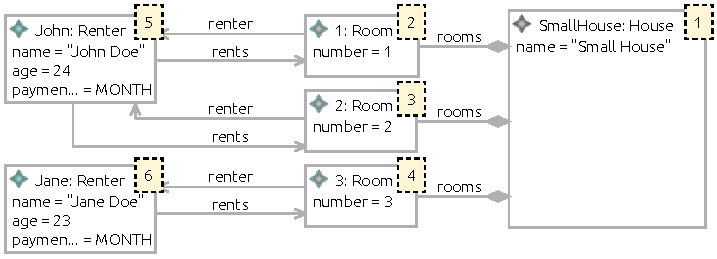
\includegraphics{images/03_formalisations/02_ecore_formalisation/instance_model_example.pdf}
        \caption{Instance model based on Ecore notation}
    \end{subfigure}
    
    \begin{subfigure}{\textwidth}
        \centering
        \begin{align*}
            Object_{Im} =\ & \{ 
                1, 2, 3, 4, 5, 6
            \}\\
            \mathrm{ObjectClass}_{Im} =\ & \{ 
                ( 1, .\type{House} ),
                ( 2, .\type{Room} ),
                ( 3, .\type{Room} ), 
                ( 4, .\type{Room} ),
                ( 5, .\type{Renter} ),
                ( 6, .\type{Renter} ),
            \}\\
            \mathrm{ObjectId}_{Im} =\ & \{ 
                ( 1, .\type{SmallHouse} ),
                ( 2, .\type{1} ),
                ( 3, .\type{2} ), 
                ( 4, .\type{3} ),
                ( 5, .\type{John} ),
                ( 6, .\type{Jane} )
            \}\\
            \mathrm{FieldValue}_{Im} =\ & \Big\{ 
                \Big( \big( 1, ( .\type{House}, \type{name} ) \big), \big[ \type{string}, \text{``Small House''} \big] \Big),\\&
                \Big( \big( 1, ( .\type{House}, \type{rooms} ) \big), \big[ \type{setof}, \big\langle [ \type{obj}, 2 ], [ \type{obj}, 3 ], [ \type{obj}, 4 ] \big\rangle \big] \Big),\\&
                \Big( \big( 2, ( .\type{Room}, \type{number} ) \big), \big[ \type{int}, 1 \big] \Big),\
                \Big( \big( 2, ( .\type{Room}, \type{renter} ) \big), \big[ \type{obj}, 5 \big] \Big),\\&
                \Big( \big( 3, ( .\type{Room}, \type{number} ) \big), \big[ \type{int}, 2 \big] \Big),
                \Big( \big( 3, ( .\type{Room}, \type{renter} ) \big), \big[ \type{obj}, 5 \big] \Big),\\&
                \Big( \big( 4, ( .\type{Room}, \type{number} ) \big), \big[ \type{int}, 3 \big] \Big),
                \Big( \big( 4, ( .\type{Room}, \type{renter} ) \big), \big[ \type{obj}, 6 \big] \Big),\\&
                \Big( \big( 5, ( .\type{Person}, \type{name} ) \big), \big[ \type{string}, \text{``John Doe''} \big] \Big),\\&
                \Big( \big( 5, ( .\type{Person}, \type{age} ) \big), \big[ \type{int}, 24 \big] \Big),\\&
                \Big( \big( 5, ( .\type{Renter}, \type{payment\_interval} ) \big), \big[ \type{enum}, ( .\type{PaymentInterval}, \type{MONTH} ) \big] \Big),\\&
                \Big( \big( 5, ( .\type{Renter}, \type{rents} ) \big), \big[ \type{setof}, \big\langle [ \type{obj}, 2 ], [ \type{obj}, 3 ] \big\rangle \big] \Big),\\&
                \Big( \big( 6, ( .\type{Person}, \type{name} ) \big), \big[ \type{string}, \text{``Jane Doe''} \big] \Big),\\&
                \Big( \big( 6, ( .\type{Person}, \type{age} ) \big), \big[ \type{int}, 23 \big] \Big),\\&
                \Big( \big( 6, ( .\type{Renter}, \type{payment\_interval} ) \big), \big[ \type{enum}, ( .\type{PaymentInterval}, \type{MONTH} ) \big] \Big),\\&
                \Big( \big( 6, ( .\type{Renter}, \type{rents} ) \big), \big[ \type{setof}, \big\langle [ \type{obj}, 4 ] \big\rangle \big] \Big)
            \Big\}\\
            \mathrm{DefaultValue}_{Im} =\ & \Big\{ 
                \Big( .\type{Constant}.\type{PaymentInterval}.\type{Month}, \big[ \type{enum}, ( .\type{PaymentInterval}, \type{MONTH} ) \big] \Big)
            \Big\}
        \end{align*}
        \caption{Formal definition of the instance model}
    \end{subfigure}
    \caption{Example of an instance model corresponding with \cref{defin:formalisations:ecore_formalisation:instance_models:instance_model}}
    \label{fig:formalisations:ecore_formalisation:instance_models:instance_model_example}
\end{figure}

An example model is represented by \cref{fig:formalisations:ecore_formalisation:instance_models:instance_model_example}. It is based on the type model from the example in \cref{fig:formalisations:ecore_formalisation:type_models:type_model_example}.
It shows 2 instantiations of the $\type{Renter}$ class: the $\type{John}$ and $\type{Jane}$ objects. Furthermore, there are three instantiations of the $\type{Room}$ class ($\type{1}$, $\type{2}$ and $\type{3}$) and one instantiation of the $\type{House}$ class ($\type{SmallHouse}$). The text after the colon in the header of each object represents the $ObjectClass_{Im}$ of each object. Additionally, the text preceding the colon represents the $ObjectId_{Im}$. The $\type{Renter}$ objects have values assigned for all fields, including the fields of their superclasses. This also holds for the $\type{Room}$ and $\type{House}$ objects. For attributes, the assignment to a field name represents the value of a field. For relations, a named arrow between two objects represents the value of the field. The name of the arrow represents the field name, and multiple arrows with the same name represent multiple values for the same field.

Note that the objects from the example are represented by elements from $\mathbb{N}^+$. The conceptual model does not give a concrete specification for elements in the $Object_{Im}$ set, but by convention objects (or in graph terms, nodes) are represented by numbers.

For each instance model, a set of possible values is defined by the values for all data types, the possible enumerations of the type model and the objects in the instance model. Each value has a symbol that defines its type, allowing the values in an instance model to be typed by the types in the type model. This symbol also allows values with identical content but a different type to be separated. For example, any value in $\mathbb{Z} \cap \mathbb{R}$ (which can be of type $\type{integer}$ or $\type{real}$). Container values aggregate multiple values, which are typed by container types.

\begin{defin}[Values]
\label{defin:formalisations:ecore_formalisation:instance_models:values}
Given any instance model $Im$, the set of values is $Value_{Im}$.

The set of values is then defined as
\begin{equation*}
    Value_{Im} = AtomValue_{Im} \cup ContainerValue_{Im}
\end{equation*}
with
\begin{itemize}
    \item $AtomValue_{Im} = ClassValue_{Im} \cup LiteralValue \cup (\{ \type{enum} \} \times EnumValue_{Tm}) \cup (\{ \type{data} \times \mathbb{S}\})$
    \item $LiteralValue = (\{ \type{bool} \} \times \mathbb{B}) \cup (\{ \type{int} \} \times \mathbb{Z}) \cup (\{ \type{real} \} \times \mathbb{R}) \cup (\{ \type{string} \} \times \mathbb{S})$
    \item $ClassValue_{Im} = \{ \type{obj} \} \times (Object_{Im} \cup { \type{nil} })$
    \item $ContainerValue_{Im} = \{ \type{setof}, \type{bagof}, \type{seqof}, \type{ordof} \} \times Value_{Im}^*$ (where $Value_{Im}^*$ allows containers to recursively contain other containers.)
\end{itemize}

The set of values is recursively defined as the smallest solution of the given set of equations for $Value_{Im}$ and $ContainerValue_{Im}$. Furthermore, elements of the set $Value_{Im}$ are written using square brackets, e.g. $[\type{string}, \text{``Example''}]$ or $[\type{setof}, \langle [\type{int}, 4], [\type{int}, 8] \rangle]$.

\isabellelref{Value}{Ecore.Instance_Model}
\end{defin}

For custom data types, the value is an element from the set $\mathbb{S}$. In Ecore, custom data types can be made serializable, which means a value from $\mathbb{S}$ can be stored for the custom data type. Thus, the value for a custom data type can be stored in the model, but it cannot be further interpreted.

Containers attributed as $\type{setof}$ or $\type{ordof}$ are considered to have unique values, whereas containers attributed as $\type{bagof}$ or $\type{seqof}$ are not. This means for example that a tuple with two or more identical values is not a valid value for a container attributed as $\type{setof}$ or $\type{ordof}$, see also \cref{defin:formalisations:ecore_formalisation:instance_models:valid_type_values}.

Additionally, the values of a container attributed as $\type{bagof}$ or $\type{setof}$ are considered unordered, and $\type{seqof}$ or $\type{ordof}$ ordered. This affects the equivalency of containers, as defined in \cref{defin:formalisations:ecore_formalisation:instance_models:value_equivalency}.

In the example, the set of atomic values that are assigned consists of
\begin{align*}
    \{&
        [ \type{string}, \text{``Small House''} ], 
        [ \type{string}, \text{``John Doe''} ], 
        [ \type{string}, \text{``Jane Doe''} ],\\&
        [ \type{int}, 1 ], 
        [ \type{int}, 2 ], 
        [ \type{int}, 3 ], 
        [ \type{int}, 24 ], 
        [ \type{int}, 23 ],\\&
        [ \type{enum}, ( .\type{PaymentInterval}, \type{MONTH} ) ]\\&
        [ \type{obj}, 5 ],
        [ \type{obj}, 6 ]
    \}
\end{align*}
Note that only the $\type{Renter}$ objects are in an atomic assigned value for the field $(.\type{Room}, \type{renter})$, as it is the only field that references a single object. All other relations in the type model are container types, and as such all the objects are contained in a container value as well. For example, the container value for the $\type{rooms}$ field of the $\type{House}$ object is $\big[ \type{setof}, \big\langle [ \type{obj}, 2 ], [ \type{obj}, 3 ], [ \type{obj}, 4 ] \big\rangle \big]$ (in no particular order, as the relation is of a set container type).

Each instance model also defines an equivalence relation for values. This relation allows the comparison of aggregate values and explicitly defines equivalency for unordered container values.

\begin{defin}[Value equivalency]
\label{defin:formalisations:ecore_formalisation:instance_models:value_equivalency}
Two values are equivalent $(\equiv_{Im}\: \subseteq Value_{Im} \times Value_{Im})$ if both the type is identical and the actual value content is equivalent. It is defined as the smallest reflexive relation between values and the relations defined by the rules given next.

For atomic values equivalence is defined as
\begin{mathpar}
    \inferrule{v_1 \in Value_{Im} \\ v_2 \in Value_{Im} \\ v_1 = v_2}{v_1 \equiv_{Im} v_2}
\end{mathpar}

Sequences and ordered sets are equivalent if the values in their tuples are pairwise equivalent.
\begin{mathpar}
    \inferrule[Sequence container equivalency]{c_1 = \big[ \type{seqof}, \langle v_1, \dotsc, v_n \rangle \big] \\ c_2 = \big[ \type{seqof}, \langle u_1, \dotsc, u_n \rangle \big] \\ v_1 \equiv_{Im} u_1, \dotsc, v_n \equiv_{Im} u_n}{c_1 \equiv_{Im} c_2}
\end{mathpar}
\begin{mathpar}
    \inferrule[Ordered set container equivalency]{c_1 = \big[ \type{ordof}, \langle v_1, \dotsc, v_n \rangle \big] \\ c_2 = \big[ \type{ordof}, \langle u_1, \dotsc, u_n \rangle \big] \\ v_1 \equiv_{Im} u_1, \dotsc, v_n \equiv_{Im} u_n}{c_1 \equiv_{Im} c_2}
\end{mathpar}

Sets and bags are equivalent if there exists a bijective function which maps elements from one set/bag
to the other, such that the mapped values are equivalent.
\begin{mathpar}
    \inferrule[Set container equivalency]{c_1 = \big[ \type{setof}, \langle v_1, \dotsc, v_n \rangle \big] \\ c_2 = \big[ \type{setof}, \langle u_1, \dotsc, u_n \rangle \big] \\ \exists f: \{1, \dotsc, n\} \bij \{1, \dotsc, n\}: v_i \equiv_{Im} u_{f(i)}}{c_1 \equiv_{Im} c_2}
\end{mathpar}
\begin{mathpar}
    \inferrule[Bag container equivalency]{c_1 = \big[ \type{bagof}, \langle v_1, \dotsc, v_n \rangle \big] \\ c_2 = \big[ \type{bagof}, \langle u_1, \dotsc, u_n \rangle \big] \\ \exists f: \{1, \dotsc, n\} \bij \{1, \dotsc, n\}: v_i \equiv_{Im} u_{f(i)}}{c_1 \equiv_{Im} c_2}
\end{mathpar}

\isabellelref{value_equiv}{Ecore.Instance_Model}
\end{defin}

In the example, the value $\big[ \type{setof}, \big\langle [ \type{obj}, 2 ], [ \type{obj}, 3 ] \big\rangle \big]$ would thus be equivalent to $\big[ \type{setof}, \big\langle [ \type{obj}, 3 ], [ \type{obj}, 2 ] \big\rangle \big]$, as the ordering does not matter for `$\type{setof}$' container types.

For each type in $Type_{Tm}$, there exists a set of values from $Value_{Im}$ which is considered \textit{valid}. This is
defined by a relation $Valid_{Im} \subseteq (Type_{Tm} \times Value_{Im})$ which defines a tuple for each valid value given a type.

\begin{defin}[Valid type values]
\label{defin:formalisations:ecore_formalisation:instance_models:valid_type_values}
The $Valid_{Im}$ set contains tuples which indicate what values are valid for a given type, which is defined by
\begin{equation*}
    Valid_{Im} \subseteq (Type_{Tm} \times Value_{Im})
\end{equation*}

An element $[ T, v ] \in Valid_{Im}$ may be written as
\begin{mathpar}
    \inferrule{\ }{v:_{Im} T}
\end{mathpar}

The contents of the $Valid_{Im}$ set is then defined as follows:

Data type values:
\begin{mathpar}
    \inferrule{v \in \mathbb{B}}{[ \type{bool}, v ]:_{Im} \type{boolean}}
    \and
    \inferrule{v \in \mathbb{Z}}{[ \type{int}, v ]:_{Im} \type{integer}}
    \and
    \inferrule{v \in \mathbb{R}}{[ \type{real}, v ]:_{Im} \type{real}}
    \and
    \inferrule{v \in \mathbb{S}}{[ \type{string}, v ]:_{Im} \type{string}}
\end{mathpar}

Class values:
\begin{mathpar}
    \inferrule{ObjectClass_{Im}(o) = c \\ !c \sqsubseteq_{Tm} t \\ t \in ClassType_{Tm}}{[ \type{obj}, o ]:_{Im} t}
    \and
    \inferrule{t \in \{ \type{nullable} \} \times Class_{Tm}}{[ \type{obj}, \type{nil} ]:_{Im} t}
\end{mathpar}

Enumeration values:
\begin{mathpar}
    \inferrule{( ename, eval ) \in EnumValue_{Tm} \\ ename \in Enum_{Tm}}{[ \type{enum}, ( ename, eval ) ]:_{Im} ename}
\end{mathpar}

User-defined data type values:
\begin{mathpar}
    \inferrule{v \in \mathbb{S} \\ t \in UserDataType_{Tm}}{[ \type{data}, v ]:_{Im} t}
\end{mathpar}

Container values:
\begin{mathpar}
    \inferrule{v_1:_{Im} T, \dotsc, v_n:_{Im} T \\ \langle v_1, \dotsc, v_n \rangle\ \mathrm{distinct} \\ [ \type{setof}, T ] \in Container_{Tm}}{[ \type{setof}, \langle v_1, \dotsc, v_n \rangle ]:_{Im} [ \type{setof}, T ]}
    \and
    \inferrule{v_1:_{Im} T, \dotsc, v_n:_{Im} T \\ [ \type{bagof}, T ] \in Container_{Tm}}{[ \type{bagof}, \langle v_1, \dotsc, v_n \rangle ]:_{Im} [ \type{bagof}, T ]}
    \and
    \inferrule{v_1:_{Im} T, \dotsc, v_n:_{Im} T \\ \langle v_1, \dotsc, v_n \rangle\ \mathrm{distinct} \\ [ \type{ordof}, T ] \in Container_{Tm}}{[ \type{ordof}, \langle v_1, \dotsc, v_n \rangle ]:_{Im} [ \type{ordof}, T ]}
    \and
    \inferrule{v_1:_{Im} T, \dotsc, v_n:_{Im} T \\ [ \type{seqof}, T ] \in Container_{Tm}}{[ \type{seqof}, \langle v_1, \dotsc, v_n \rangle ]:_{Im} [ \type{seqof}, T ]}
\end{mathpar}

\isabellelref{Valid}{Ecore.Instance_Model}
\end{defin}

The validity of an instance model depends on the multiplicity of field values. The valid multiplicities depend on the types and field signatures in the corresponding type model. As a consequence, a valid multiplicity also requires the type of the value to be valid. The multiplicity is of most influence for container values, as they can contain an arbitrary amount of values.

\begin{defin}[Multiplicity validity]
\label{defin:formalisations:ecore_formalisation:instance_models:multiplicity_validity}
A field value $( ( object, field ), value ) \in FieldValue_{Im}$ has a valid multiplicity if the following property holds:
\begin{multline*}
    value:_{Im} \mathrm{type}_{Tm}(field) \land value = [ t, \langle v_1, \dotsc, v_n \rangle ] \in ContainerValue_{Im} \Longrightarrow\\ \mathrm{lower}_{Im}(field) \leq n \leq \mathrm{upper}_{Im}(field)
\end{multline*}

This may be written as $\mathrm{validMul}_{Im}\big((( object, field ), value)\big)$.

\isabellelref{validMul}{Ecore.Instance_Model}
\end{defin}

\begin{figure}
    \centering
    \begin{subfigure}{\textwidth}
        \centering
        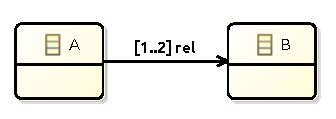
\includegraphics{images/03_formalisations/02_ecore_formalisation/multiplicities/type_model.pdf}
        \caption{Example type model}
        \label{fig:formalisations:ecore_formalisation:instance_models:multiplicity_example:type_model}
    \end{subfigure}
    
    \begin{subfigure}{0.3\textwidth}
        \centering
        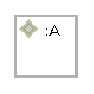
\includegraphics{images/03_formalisations/02_ecore_formalisation/multiplicities/invalid_lower.pdf}
        \caption{Invalid instance model: cardinality of $\type{rel}$ too low}
        \label{fig:formalisations:ecore_formalisation:instance_models:multiplicity_example:invalid_lower}
    \end{subfigure}
    \begin{subfigure}{0.3\textwidth}
        \centering
        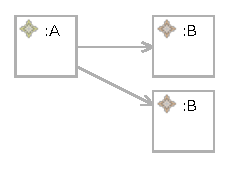
\includegraphics{images/03_formalisations/02_ecore_formalisation/multiplicities/valid.pdf}
        \caption{Valid instance model: cardinality of $\type{rel}$ within bounds}
        \label{fig:formalisations:ecore_formalisation:instance_models:multiplicity_example:valid}
    \end{subfigure}
    \begin{subfigure}{0.3\textwidth}
        \centering
        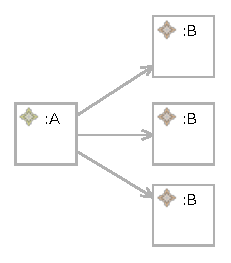
\includegraphics{images/03_formalisations/02_ecore_formalisation/multiplicities/invalid_upper.pdf}
        \caption{Invalid instance model: cardinality of $\type{rel}$ too high}
        \label{fig:formalisations:ecore_formalisation:instance_models:multiplicity_example:invalid_upper}
    \end{subfigure}
    \caption{Examples of valid and invalid multiplicities}
    \label{fig:formalisations:ecore_formalisation:instance_models:multiplicity_example}
\end{figure}

The examples shown in \cref{fig:formalisations:ecore_formalisation:instance_models:multiplicity_example} show different multiplicities in instance models. More specifically, \cref{fig:formalisations:ecore_formalisation:instance_models:multiplicity_example:type_model} shows a type model that specifies a multiplicity of $1..2$ for the $\type{rel}$ relation. \cref{fig:formalisations:ecore_formalisation:instance_models:multiplicity_example:invalid_lower} and \cref{fig:formalisations:ecore_formalisation:instance_models:multiplicity_example:invalid_upper} show two instance models that have an invalid multiplicity (too low and too high respectively), whereas \cref{fig:formalisations:ecore_formalisation:instance_models:multiplicity_example:valid} shows an instance model with correct multiplicity (an alternative correct instance model could have only a single instance of class $\type{B}$).

In order to simplify reasoning over assignments of values, the $\mathrm{edgeCount}$ and $\mathrm{edge}$ operators are defined. These operators specify the number of relations (and the existence thereof) between any two objects.

\begin{defin}[Value edges]
\label{defin:formalisations:ecore_formalisation:instance_models:value_edges}
Let $a, b \in Object_{Im}$ and $r \in Field_{Tm}$ where $r \in fields_{Tm}(\mathrm{ObjectClass}_{Im}(a))$. Furthermore, we define $\mathrm{containerCount}_{Im}(a, r, b)$ as
\begin{equation*}
    \mathrm{containerCount}_{Im}(a, r, b) = \big|\big\{ i \in \mathbb{N} \mid \big( (a, r), \big[ t, \langle v_1, \dotsc, v_n \rangle \big] \big) \in \mathrm{FieldValue}_{Im} \land v_i = [ \type{obj}, b ] \big\}\big|
\end{equation*}

Then $\mathrm{edgeCount}_{Im}(a, r, b)$ is defined as
\begin{equation*}
    \mathrm{edgeCount}_{Im}(a, r, b) = 
    \begin{cases}
        0, & \begin{aligned} 
            \text{if } &\mathrm{type}_{Tm}(r) \not\in Container_{Tm} \\&\land \big( (a, r), [ \type{obj}, b ] \big) \not\in \mathrm{FieldValue}_{Im}
        \end{aligned}\\
        1, & \begin{aligned} 
            \text{if } &\mathrm{type}_{Tm}(r) \not\in Container_{Tm} \\&\land \big( (a, r), [ \type{obj}, b ] \big) \in \mathrm{FieldValue}_{Im}
        \end{aligned}\\
        \mathrm{containerCount}_{Im}(a, r, b), & \text{otherwise}
    \end{cases}
\end{equation*}
\isabellelref{edgeCount}{Ecore.Instance_Model}

The $\mathrm{edge}_{Im}(a, r, b)$ predicate is defined as
\begin{equation*}
    \mathrm{edge}_{Im}(a, r, b) = \mathrm{edgeCount}_{Im}(a, r, b) \geq 1
\end{equation*}
\isabellelref{edge}{Ecore.Instance_Model}
\end{defin}

As previously mentioned, the properties specified in a type model must be satisfied by the instance model in order for it to be valid. For each property, there is a satisfaction formula defined, which must hold for a given instance model for that instance model to be valid. The following definition specifies such a formula for each possible property in a type model.

\begin{defin}[Property satisfaction]
\label{defin:formalisations:ecore_formalisation:instance_models:property_satisfaction}
Given an instance model $Im$ and a type model $Tm$, a property $p \in Prop_{Tm}$ can be satisfied, written
as $Im \models p$, if the satisfaction formula holds for $p$.

\begin{itemize}
    \item The abstract property $[ \type{abstract}, c ]$ is satisfied by some instance model $Im$ if none of the objects in $Im$ is typed by class $c$.
    
    Formally, the satisfaction formula for $Im \models [ \type{abstract}, c ]$ is defined as:
    \begin{equation*}
        \nexists o \in Object_{Im}: \mathrm{ObjectClass}_{Im}(o) = c
    \end{equation*}

    \item The containment property $[ \type{containment}, r ]$ is satisfied for an instance model $Im$ when any object in $Im$ that is the target for a containment relation is contained by no more than one object, and there are no cycles in the instance model given the containment values.
    
    Let $CR_{Tm} = \{r \mid r \in Rel_{Tm} \land [ \type{containment}, r ] \in Prop_{Tm} \}$ be the set of all containment relations in a type model $Tm$. The satisfaction formula for $Im \models [ \type{containment}, r ]$ is then defined as:
    \begin{align*}
        \forall o \in\ &Object_{Im}\!: \big|\big\{ \big( ( f\!o, f\!\!f ), f\!v \big) \mid \big( ( f\!o, f\!\!f ), f\!v \big) \in \mathrm{FieldValue}_{Im} \land [ \type{obj}, o ] = f\!v \land f\!\!f \in CR_{Tm} \big\}\big| \leq 1 \\&
        \land \big\{ (f\!o, f\!v) \mid \big( ( f\!o, f\!\!f ), f\!v \big) \in \mathrm{FieldValue}_{Im} \land f\!\!f \in CR_{Tm} \big\} \text{ is acyclic}
    \end{align*}
    
    \item The identity property $[ \type{identity}, c, A ]$. is satisfied for an instance model $Im$, when for each pair of objects of class $c$, the values for at least one of the attributes in $A$ is different.
    
    Formally, the satisfaction formula for $Im \models [ \type{identity}, c, A ]$ is defined as:
    \begin{align*}
        \forall o, o' \in\ &Object_{Im}\!: \mathrm{ObjectClass}_{Im}(o) = c \land \mathrm{ObjectClass}_{Im}(o') = c \\&\land \forall a \in A\!: \mathrm{FieldValue}_{Im}(( o, a )) \equiv_{Im} \mathrm{FieldValue}_{Im}(( o', a )) \\&\Longrightarrow o = o'
    \end{align*}
    
    \item The keyset property $[ \type{keyset}, r, A ]$ is satisfied for an instance model $Im$ when for each object containing relation $r$, each pair of objects referenced by $r$ has a different set of values for the attributes in $A$. In other words, for each such pair, there is at least one value for the attributes in $A$ that is different for both objects.
    
    The satisfaction formula for $Im \models [ \type{keyset}, r, A ]$ is defined as:
    \begin{align*}
        \forall o, o', p \in\ &Object_{Im}\!: r \in \mathrm{fields}_{Tm}(\mathrm{ObjectClass}_{Im}(p))\\&
        \land \mathrm{edge}_{Im}(p, r, o) \land \mathrm{edge}_{Im}(p, r, o')\\&
        \land \forall a \in A\!: \mathrm{FieldValue}_{Im}(( o, a )) \equiv_{Im} \mathrm{FieldValue}_{Im}(( o', a )) \\& \Longrightarrow o = o'
    \end{align*}
    
    \item The opposite property $[ \type{opposite}, r, r' ]$ is satisfied for an instance model $Im$ when for each object $o$ with a value for $r$, the referenced objects by $r$ have a value for $r'$, which references object $o$. In other words: each object referenced by $r$ must also have a reference $r'$ that references the source object that defined $r$.
    
    Formally, the satisfaction formula for $Im \models [ \type{opposite}, r, r' ]$ given an instance is defined as:
    \begin{align*}
        \forall o, o' \in Object_{Im}\!: \mathrm{edgeCount}_{Im}(o, r, o') = \mathrm{edgeCount}_{Im}(o', r', o)
    \end{align*}
\end{itemize}

\isabellelref{property_satisfaction}{Ecore.Instance_Model}
\end{defin}

\begin{figure}
    \centering
    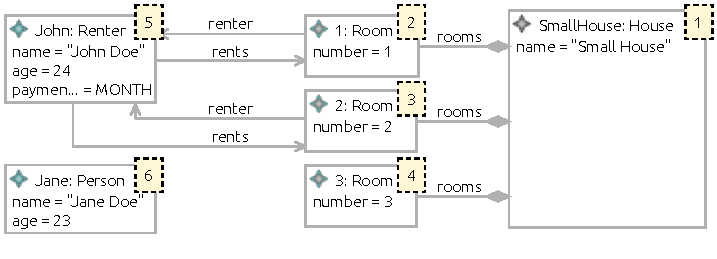
\includegraphics{images/03_formalisations/02_ecore_formalisation/properties/invalid_abstract.pdf}
    \caption{Model not satisfying the $\type{abstract}$ property.}
    \label{fig:formalisations:ecore_formalisation:instance_models:properties:abstract}
\end{figure}

\cref{fig:formalisations:ecore_formalisation:instance_models:instance_model_example} shows an example of an instance model that satisfies the $[ \type{abstract}, \type{Person} ]$ property, as no direct instantiations of the $\type{Person}$ class exist. On the other hand, \cref{fig:formalisations:ecore_formalisation:instance_models:properties:abstract} shows an instance model that does not satisfy the property, as the $\type{Person}$ class has been instantiated (by the object $\type{Jane}$).

\begin{figure}[p]
    \centering
    \begin{subfigure}{0.35\textwidth}
        \centering
        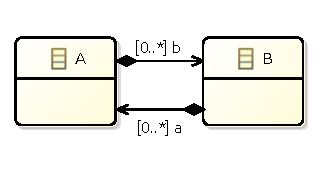
\includegraphics{images/03_formalisations/02_ecore_formalisation/properties/containment/type_model.pdf}
        \caption{Example type model with two containment relations}
        \label{fig:formalisations:ecore_formalisation:instance_models:properties:containment:type_model}
    \end{subfigure}
    \begin{subfigure}{0.3\textwidth}
        \centering
        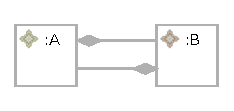
\includegraphics{images/03_formalisations/02_ecore_formalisation/properties/containment/invalid.pdf}
        \caption{Model not satisfying the containment property}
        \label{fig:formalisations:ecore_formalisation:instance_models:properties:containment:invalid}
    \end{subfigure}
    \begin{subfigure}{0.3\textwidth}
        \centering
        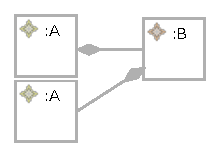
\includegraphics{images/03_formalisations/02_ecore_formalisation/properties/containment/valid.pdf}
        \caption{Model satisfying the containment property}
        \label{fig:formalisations:ecore_formalisation:instance_models:properties:containment:valid}
    \end{subfigure}
    \caption{Examples of the $\type{containment}$ property.}
    \label{fig:formalisations:ecore_formalisation:instance_models:properties:containment}
\end{figure}

\cref{fig:formalisations:ecore_formalisation:instance_models:properties:containment:type_model} shows a type model that defines two containment relations, in opposite direction. The instance model given in \cref{fig:formalisations:ecore_formalisation:instance_models:properties:containment:invalid} does not satisfy the satisfaction formula for the containment property, as there exists a cycle of containment relations. This is corrected in the instance model in \cref{fig:formalisations:ecore_formalisation:instance_models:properties:containment:valid}, where such a cycle does not exist (and each object is containment by at most one other object).

\begin{figure}[p]
    \centering
    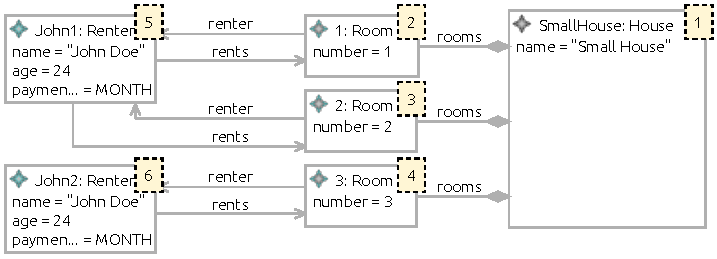
\includegraphics{images/03_formalisations/02_ecore_formalisation/properties/invalid_identity.pdf}
    \caption{Model not satisfying the $\type{identity}$ property.}
    \label{fig:formalisations:ecore_formalisation:instance_models:properties:identity}
\end{figure}

To illustrate the satisfaction of a $\textsf{identity}$ property, assume the type model in \cref{fig:formalisations:ecore_formalisation:type_models:type_model_example} specifies an identity property for the $\type{name}$ and $\type{age}$ attributes of the $\type{Renter}$ object. Formally, we define the following property:
\begin{equation*}
  \big[ \textsf{identity}, .\type{Renter}, \big\{ ( .\type{Person}, \type{name} ), ( .\type{Person}, \type{age} ) \big\} \big]  
\end{equation*}

The example in \cref{fig:formalisations:ecore_formalisation:instance_models:properties:identity} shows an instance model that does not satisfy the property, as the $\type{Renter}$ objects share the same values for the $\type{name}$ and $\type{age}$ attributes, but are still identified as different objects. In \cref{fig:formalisations:ecore_formalisation:instance_models:instance_model_example} the values of the $\type{name}$ and $\type{age}$ attributes are not the same, and thus the property would be satisfied.

\begin{figure}[p]
    \centering
    \begin{subfigure}{0.45\textwidth}
        \centering
        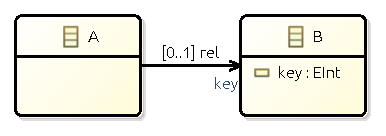
\includegraphics{images/03_formalisations/02_ecore_formalisation/properties/keyset/type_model.pdf}
        \caption{Example type model with relation $\type{rel}$ that has the keyset property defined on field $\type{key}$}
        \label{fig:formalisations:ecore_formalisation:instance_models:properties:keyset:type_model}
    \end{subfigure}
    \begin{subfigure}{0.25\textwidth}
        \centering
        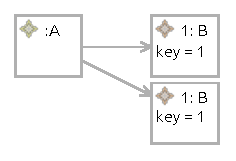
\includegraphics{images/03_formalisations/02_ecore_formalisation/properties/keyset/invalid.pdf}
        \caption{Model not satisfying the keyset property}
        \label{fig:formalisations:ecore_formalisation:instance_models:properties:keyset:invalid}
    \end{subfigure}
    \begin{subfigure}{0.25\textwidth}
        \centering
        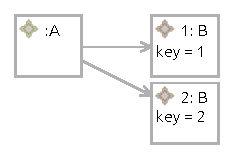
\includegraphics{images/03_formalisations/02_ecore_formalisation/properties/keyset/valid.pdf}
        \caption{Model satisfying the keyset property}
        \label{fig:formalisations:ecore_formalisation:instance_models:properties:keyset:valid}
    \end{subfigure}
    \caption{Examples of the $\type{keyset}$ property.}
    \label{fig:formalisations:ecore_formalisation:instance_models:properties:keyset}
\end{figure}

An example of the keyset property is shown in \cref{fig:formalisations:ecore_formalisation:instance_models:properties:keyset}. In \cref{fig:formalisations:ecore_formalisation:instance_models:properties:keyset:type_model}, we see the type model of this example. We assume there exists a class $\type{A}$ which can reference objects of class $\type{B}$ through relation $\type{rel}$. Furthermore, we assume that the $\type{key}$ field on class $\type{B}$ is used as key for the relation $\type{rel}$. In that case, \cref{fig:formalisations:ecore_formalisation:instance_models:properties:keyset:invalid} shows a violation of the $\type{keyset}$ property, because the 2 objects of type $\type{B}$ have the same value for $\type{key}$. In \cref{fig:formalisations:ecore_formalisation:instance_models:properties:keyset:valid}, the property is satisfied as both objects of type $\type{B}$ have a different value for $\type{key}$.

\begin{figure}[p]
    \centering
    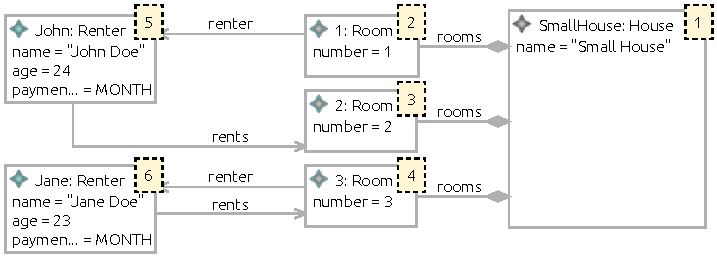
\includegraphics{images/03_formalisations/02_ecore_formalisation/properties/invalid_opposite.pdf}
    \caption{Model not satisfying the $\type{opposite}$ property.}
    \label{fig:formalisations:ecore_formalisation:instance_models:properties:opposite}
\end{figure}

In \cref{fig:formalisations:ecore_formalisation:instance_models:properties:opposite}, an example model is shown which does not satisfy the opposite property for the $\type{rents}$ and $\type{renter}$ relations. Although the number of relations is equal, they do not have the same source and target objects (in opposite direction). The example model in \cref{fig:formalisations:ecore_formalisation:instance_models:instance_model_example} does in fact satisfy the property.

With the previous definitions, it is now possible to define when an instance model itself is valid, given its type model.

\begin{defin}[Model validity]
\label{defin:formalisations:ecore_formalisation:instance_models:model_validity}
An instance model $Im$ is said to be valid with respect to type model $Tm$ if and only if
\begin{itemize}
    \item All values are correctly typed: $\forall ( ( obj, f\!ield ), val ) \in \mathrm{FieldValue}_{Im}\!: val:_{Im} \mathrm{type}_{Tm}(f\!ield)$.
    \item All container multiplicities are valid: $\forall fv \in \mathrm{FieldValue}_{Im}\!: \mathrm{validMul}_{Im}(f\!v)$.
    \item All properties are satisfied: $\forall p \in Prop_{Tm}\!: Im \models p$
    \item All default values have the correct type: $\forall c \in Constant_{Tm}\!: \mathrm{DefaultValue}_{Im}(c):_{Im} \mathrm{ConstType}_{Tm}(c)$.
    \item $Tm$ is consistent, as defined in \cref{defin:formalisations:ecore_formalisation:type_models:type_model_consistency}.
\end{itemize}

The validity of $Im$ with respect to $Tm$ is written as $Tm \vdash Im$.
\isabellelref{instance_model}{Ecore.Instance_Model}
\end{defin}
\section{GROOVE formalisation}
\label{sec:formalisations:groove_formalisation}

This section discusses a (partial) formalisation of GROOVE. This formalisation is limited to type graphs and instance graphs, as discussed in \cref{sec:background:groove}. These are the only GROOVE graph types that are relevant to this thesis.

\subsection{Definitions}
\label{subsec:formalisations:groove_formalisation:definitions}
This section discusses some definitions specific to the GROOVE formalisation. The definitions need to be in place before the formalisations of the different GROOVE graphs are given.

GROOVE internally uses a set of labels $Lab$ for each defined grammar. These labels are used by multiple graph types of GROOVE, including (but not limited to) type graphs and instance graphs.

\begin{defin}[Labels]
\label{defin:formalisations:groove_formalisation:definitions:labels}
$Lab$ is the set of labels used by GROOVE graphs. It can be subdivided into three sets:
\begin{itemize}
    \item The set of type labels $Lab_t \subseteq Lab$
    \item The set of edge labels $Lab_e \subseteq Lab$
    \item The set of flag labels $Lab_f \subseteq Lab$
\end{itemize}

The intersection of each of the sets $Lab_t$, $Lab_f$ and $Lab_e$ has to be empty:
\begin{equation*}
    Lab_t \cap Lab_f = \emptyset \land Lab_t \cap Lab_e = \emptyset \land Lab_f \cap Lab_e = \emptyset
\end{equation*}

\isabellelref{Lab}{GROOVE.Type_Graph}
\end{defin}

The set $Lab_t$ will be used to denote the types of nodes in the graph, while the $Lab_e$ set will be used to distinguish between different edges. The $Lab_f$ set are labels for particular kind of edges which always have an identical source and target node. These are used as flags on nodes to indicate that a specific property holds for a node.

Although the intersection of each of the sets $Lab_t$, $Lab_f$ and $Lab_e$ has to be empty, the sets do not necessarily form a partition of $Lab$, as one or more of the subsets can be empty. Furthermore, $Lab$ itself can be empty if the GROOVE grammar does not define any types, flags or edge labels.

Besides $Lab$ that belongs to a grammar, GROOVE uses a set of reserved primitive type labels $Lab_{prim}$ that can never be part of the label set of a grammar.

\begin{defin}[Primitive type labels]
\label{defin:formalisations:groove_formalisation:definitions:primitive_type_labels}
GROOVE has a set of reserved primitive type labels $Lab_{prim}$:
\begin{equation*}
    Lab_{prim} = \{ \type{bool}, \type{int}, \type{real}, \type{string} \}
\end{equation*}

It should hold that $Lab \cap Lab_{prim} = \emptyset$ since the primitive type labels are reserved.
\end{defin}

The primitive type labels allow the use of primitive types as attributes and values. The label $\type{bool}$ represents the type for boolean values $\mathbb{B}$, $\type{int}$ represents the type for integer values $\mathbb{Z}$, $\type{real}$ represents the type for real numbers $\mathbb{R}$ and finally $\type{string}$ represents the type for string values $\mathbb{S}$.
\subsection{Type graphs}
\label{subsec:formalisations:groove_formalisation:type_graphs}

In GROOVE, type graphs are used to constrain the valid instance graphs within the grammar. From a type graph follows a set of valid instance graphs that can be used for verification.

\begin{defin}[Type graph]
\label{defin:formalisations:groove_formalisation:type_graphs:type_graph}
A type graph is modeled as tuple $TG$:
\begin{equation}
    TG = \langle NT, ET, \sqsubseteq, abs, \mathrm{mult}, contains \rangle
\end{equation}
with
\begin{itemize}
    \item $NT \subseteq Lab_t \cup Lab_{prim}$ is the set of nodes in the type graph. The nodes can consist of type labels (see \cref{defin:formalisations:groove_formalisation:definitions:labels}) or primitive type labels (see \cref{defin:formalisations:groove_formalisation:definitions:primitive_type_labels}).
    
    \item $ET \subseteq NT \times (Lab_e \cup Lab_f) \times NT$ is the set of (directed) edges in the type graph, which is a set of triples containing the source and target node, as well as the edge label or flag label (see \cref{defin:formalisations:groove_formalisation:definitions:labels}) used to identify the edge.
    
    \item $\sqsubseteq\ \subseteq NT \times NT$ is the inheritance relation, the set of tuples of nodes between which an inheritance relation exists.
    
    \item $abs \subseteq NT$ is the (possibly empty) subset of nodes in the type graph which are considered abstract. An instance graph cannot instantiate abstract nodes.
    
    \item $\mathrm{mult}: ET \Rightarrow \mathbb{M} \times \mathbb{M}$ is the function which maps edges to their multiplicity pair. See \cref{defin:formalisations:groove_formalisation:type_graphs:multiplicity_pair} for the definition.
    
    \item $contains \subseteq ET$ is the set of edges which identify an containment relation. 
\end{itemize}

\isabellelref{type_graph}{GROOVE.Type_Graph}
\end{defin}

\begin{figure}[p]
    \centering
    \begin{subfigure}{\textwidth}
        \centering
        \input{images/03_formalisations/03_groove_formalisation/type_graph_example.tikz}
        \caption{Type graph in GROOVEs visual notation. Multiplicities are omitted for clarity.}
    \end{subfigure}
    
    \begin{subfigure}{\textwidth}
        \centering
        \begin{align*}
            NT_{TG} =\ & \{ 
                \type{House},
                \type{PaymentInterval},
                \type{PaymentInterval\$MONTH},\\&
                \type{PaymentInterval\$QUARTER},
                \type{Person},
                \type{Renter},
                \type{Room},
                \type{int},
                \type{string}
            \}\\
            ET_{TG} =\ & \{ 
                ( \type{House}, \type{name}, \type{string} ),
                ( \type{House}, \type{rooms}, \type{Room} ),\\&
                ( \type{Person}, \type{age}, \type{int} ),
                ( \type{Person}, \type{name}, \type{string} ),\\&
                ( \type{Renter}, \type{payment\_interval}, \type{PaymentInterval} ),
                ( \type{Renter}, \type{rents}, \type{Room} ),\\&
                ( \type{Room}, \type{number}, \type{int} ),
                ( \type{Room}, \type{renter}, \type{Renter} )
            \}\\
            \sqsubseteq_{TG}\: =\ & \{ 
                ( \type{House}, \type{House} ),
                ( \type{PaymentInterval}, \type{PaymentInterval} ),\\&
                ( \type{PaymentInterval\$MONTH}, \type{PaymentInterval} ),\\&
                ( \type{PaymentInterval\$MONTH}, \type{PaymentInterval\$MONTH} ),\\&
                ( \type{PaymentInterval\$QUARTER}, \type{PaymentInterval} ),\\&
                ( \type{PaymentInterval\$QUARTER}, \type{PaymentInterval\$QUARTER} ),\\&
                ( \type{Person}, \type{Person} ),
                ( \type{Renter}, \type{Person} ),
                ( \type{Renter}, \type{Renter} ),
                ( \type{Room}, \type{Room} ),
                ( \type{int}, \type{int} ),
                ( \type{string}, \type{string} )
            \}\\
            abs_{TG} =\ & \{ 
                \type{PaymentInterval}, \type{Person}
            \}\\
            \mathrm{mult}_{TG} =\ & \big\{ 
                \big( ( \type{House}, \type{name}, \type{string} ), ( 0..*, 1..1 ) \big),
                \big( ( \type{House}, \type{rooms}, \type{Room} ), ( 1..1, 1..* ) \big),\\&
                \big( ( \type{Person}, \type{age}, \type{int} ), ( 0..*, 1..1 ) \big),
                \big( ( \type{Person}, \type{name}, \type{string} ), ( 0..*, 1..1 ) \big),\\&
                \big( ( \type{Renter}, \type{payment\_interval}, \type{PaymentInterval} ), ( 0..*, 1..1 ) \big),\\&
                \big( ( \type{Renter}, \type{rents}, \type{Room} ), ( 0..*, 0..* ) \big),\\&
                \big( ( \type{Room}, \type{number}, \type{int} ), ( 0..*, 1..1 ) \big),
                \big( ( \type{Room}, \type{renter}, \type{Renter} ), ( 0..*, 0..1 ) \big)
            \big\}\\
            contains_{TG} =\ & \{ 
                ( \type{House}, \type{rooms}, \type{Room} )
            \}
        \end{align*}
        \caption{Formal definition of the type graph}
    \end{subfigure}
    \caption{Example of a type graph corresponding with \cref{defin:formalisations:groove_formalisation:type_graphs:type_graph}}
    \label{fig:formalisations:groove_formalisation:type_graphs:type_graph_example}
\end{figure}

An example of a type graph is given in \cref{fig:formalisations:groove_formalisation:type_graphs:type_graph_example}. This example is similar to the type model example discussed in \cref{subsec:formalisations:ecore_formalisation:type_models}. There is a node $\type{House}$ which contains $\type{Room}$s. A $\type{House}$ also has an edge to a primitive type label $\type{string}$ under edge label $\type{name}$ which represents the name of the house. Please note that in the visual representation, syntactic sugar is used to represent this edge. Instead of an extra node and edge, it is represented as part of the $\type{House}$ node. This syntactic sugar can be used for edges to primitive types and are in reality still treated as an edge to a separate node type. A $\type{Room}$ has an edge $\type{number}$, targeting the primitive type label $\type{int}$, which represents the number of the room within the house. A $\type{Room}$ can be rented by a $\type{Renter}$. The $\type{Renter}$s have edges to the $\type{Room}$s they rented under the edge label $\type{rents}$, while a $\type{Room}$ can access its $\type{Renter}$ through the edge with edge label $\type{renter}$. A $\type{Renter}$ extends the abstract $\type{Person}$ node type, which has 2 edges $\type{age}$ and $\type{name}$, targeting the primitive type labels $\type{int}$ and $\type{string}$ respectively. These edges represent the age and the name of the $\type{Person}$. Finally, a $\type{Renter}$ has an edge under the edge label $\type{payment\_interval}$, which points to a $\type{PaymentInterval}$ node type. This node type is abstract and the edge should therefore point to one of its subtypes, $\type{PaymentInterval\$MONTH}$ or $\type{PaymentInterval\$QUARTER}$. This represents the interval in which the $\type{Renter}$ pays the rent. 
Notable from the definition is that the nodes set $N$ can contain primitive type labels. As a consequence, primitive type labels need to be added explicitly to a type graph in order to use primitive type values in an instance graph.

Furthermore, each edge has a multiplicity pair tied to it, which is defined as the $\mathrm{mult}$ function in the type graph definition. The multiplicity pair consists of an incoming multiplicity and an outgoing multiplicity. The incoming multiplicity determines the allowed amount of nodes that share the same target node with this edge type. On the other hand, the outgoing multiplicity determines the number of edges a single source node may have to its target nodes.

\begin{defin}[Multiplicity pair]
\label{defin:formalisations:groove_formalisation:type_graphs:multiplicity_pair}
A multiplicity pair is defined as a tuple of two multiplicities, $\mathbb{M} \times \mathbb{M}$, in which the first value denotes the incoming multiplicity and the second value the outgoing multiplicity.

For any multiplicity pair, we define two functions:
\begin{align*}
    \mathrm{in}\!:&\: \mathbb{M} \times \mathbb{M} \Rightarrow \mathbb{M} \\
    \mathrm{out}\!:&\: \mathbb{M} \times \mathbb{M} \Rightarrow \mathbb{M}
\end{align*}
The $\mathrm{in}$ function being the function which from a multiplicity pair returns the incoming multiplicity and the $\mathrm{out}$ function being the function that returns the outgoing multiplicity, so:
\begin{equation*}
\forall m = (m_{in}, m_{out}) \in \mathrm{mult}_{TG}: \mathrm{in}(m) = m_{in} \land \mathrm{out}(m) = m_{out}  
\end{equation*}

\isabellelref{multiplicity_pair}{GROOVE.Multiplicity_Pair}
\end{defin}

With all definitions in place, it is possible to define a valid type graph.
The definition of a valid type graph introduces some new constraint that should hold for a type graph to be valid.

\begin{defin}[Type graph validity]
\label{defin:formalisations:groove_formalisation:type_graphs:type_graph_validity}
For a type graph to be valid, the following properties must hold:
\begin{enumerate}
    \item There may not be any ambiguity in the use of edges: $\forall (s_1, l, t_1) \in ET_{TG}\,\land\, (s_2, l, t_2) \in ET_{TG}\!: \big((s_1, s_2) \in\ \sqsubseteq_{TG} \lor\ (s_2, s_1) \in\ \sqsubseteq_{TG}\!\!\big) \land \big((t_1, t_2) \in\ \sqsubseteq_{TG} \lor\ (t_2, t_1) \in\ \sqsubseteq_{TG}\!\!\big) \Longrightarrow s_1 = s_2 \land t_1 = t_2$.
    \item Flags should have the same source and target node: $\forall (s, l, t) \in ET_{TG}: l \in Lab_f \Longrightarrow s = t$.
    \item $\sqsubseteq_{TG}$ is a partial order ($\sqsubseteq_{TG}$ is reflexive, transitive and anti-symmetric on $N\!$).
    \item The incoming multiplicities of edges that identify a containment relation are valid: $\forall e \in contains_{TG}: \mathrm{in}(\mathrm{mult}_{TG}(e)) = (0, 1) \lor \mathrm{in}(\mathrm{mult}_{TG}(e)) = (1, 1)$.
\end{enumerate}

\isabellelref{type_graph}{GROOVE.Type_Graph}
\end{defin}

\begin{figure}
    \centering
    \begin{subfigure}{0.45\textwidth}
        \centering
        \input{images/03_formalisations/03_groove_formalisation/edge_ambiguity_example_valid.tikz}
        \caption{Valid type graph without ambiguity}
        \label{fig:formalisations:groove_formalisation:type_graphs:ambiguous_edges_example:valid}
    \end{subfigure}
    \begin{subfigure}{0.45\textwidth}
        \centering
        \input{images/03_formalisations/03_groove_formalisation/edge_ambiguity_example_invalid.tikz}
        \caption{Invalid type graph with an ambiguous edge type labelled $\type{f}$}
        \label{fig:formalisations:groove_formalisation:type_graphs:ambiguous_edges_example:invalid}
    \end{subfigure}
    \caption{Example of ambiguity within edge types}
    \label{fig:formalisations:groove_formalisation:type_graphs:ambiguous_edges_example}
\end{figure}

The last 3 properties presented here are mostly self-explanatory. The first property might be unclear at first. This property prevents type graphs from having ambiguous edge types. \cref{fig:formalisations:groove_formalisation:type_graphs:ambiguous_edges_example} shows an example of such an ambiguity. In essence, when creating edges within an instance graph, there should be an unique solution for typing the edge. In \cref{fig:formalisations:groove_formalisation:type_graphs:ambiguous_edges_example:valid}, this is always the case, even though both edges are labelled $\type{f}$. If an edge labelled $\type{f}$ references a node of type $\type{B}$, then the edge type should be $( \type{Y}, \type{f}, \type{B} )$. When an edge labelled $\type{f}$ references a node of type $\type{A}$, the edge type should be $( \type{X}, \type{f}, \type{A} )$. There is no ambiguity possible. 

\cref{fig:formalisations:groove_formalisation:type_graphs:ambiguous_edges_example:invalid} shows an example of a type graph where ambiguity is possible. When a node of type $\type{Y}$ references a node of $\type{B}$ using an edge labelled $\type{f}$, it is unclear which edge type was meant. Both $( \type{Y}, \type{f}, \type{B} )$ and $( \type{X}, \type{f}, \type{A} )$ would be valid edge types here. This means there is ambiguity in how edges are typed. The first property of \cref{defin:formalisations:groove_formalisation:type_graphs:type_graph_validity} excludes this case, since $( \type{Y}, \type{f}, \type{B} )$ and $( \type{X}, \type{f}, \type{A} )$ are both edge types, while $(\type{Y}, \type{X}) \in\ \sqsubseteq_{TG}$ and $(\type{B}, \type{A}) \in\ \sqsubseteq_{TG}$. Then according to the first property, $\type{Y}$ should be equal to $\type{X}$ and $\type{B}$ should be equal to $\type{A}$, which is not the case, so \cref{fig:formalisations:groove_formalisation:type_graphs:ambiguous_edges_example:invalid} violates the first property, hence the example is invalid.
\subsection{Instance graphs}
\label{subsec:formalisations:groove_formalisation:instance_graphs}
Before giving a formal definition of instance graphs, the set $Node$ for a grammar needs to be defined. $Node$ is the set of possible nodes that can be part of an instance graph.

\begin{defin}[Node]
\label{defin:formalisations:groove_formalisation:instance_graphs:node}
We define a set $Node$ containing all possible instance nodes. $Node$ can be subdivided into two disjoint and covering sets
\begin{itemize}
    \item $Node_t$ is the set of typed nodes for every label in $Lab_t$
    \item $Node_v$ is the set of typed nodes for every label in $Lab_{prim}$
\end{itemize}

By definition, there exists a mapping for each element in $Node_t$ to an element in $Lab_t$ and a mapping for each element in $Node_v$ to $Lab_{prim}$. We call the mapping $\mathrm{nodeType}$:
\begin{equation*}
    \mathrm{nodeType}: (Node_t \Rightarrow Lab_t) \cup (Node_v \Rightarrow Lab_{prim})
\end{equation*}

Furthermore, the set $Node_v$ can also be mapped to actual data values in GROOVE by the function $value$.
\begin{equation*}
    \mathrm{value}: Node_v \bij \mathbb{B} \cup \mathbb{Z} \cup \mathbb{R} \cup \mathbb{S}
\end{equation*}

\isabellelref{Node}{GROOVE.Instance_Graph}
\end{defin}

Besides the set of nodes, GROOVE also has a set $Id$, which is a set of identifiers that can be used to assign each node a unique identifier.

\begin{defin}[Identifiers]
\label{defin:formalisations:groove_formalisation:instance_graphs:identifiers}
Define a global set $Id$ which consists of unique identifiers.
\end{defin}

With these definitions, it is possible to define an instance graph in GROOVE.

\begin{defin}[Instance graph]
\label{defin:formalisations:groove_formalisation:instance_graphs:instance_graph}
An instance graph corresponding to a type graph $TG$ is modeled as tuple $IG$:
\begin{equation}
    IG = \langle N, E, ident \rangle
\end{equation}
where
\begin{itemize}
    \item $N \subseteq Node_t \cup Node_v$ is the set of nodes in the instance graph.
    
    \item $E \subseteq N \times ET_{TG} \times N$ is the set of edges in the instance graph. They consist of a source and target node from $N$ and are typed by an edge from the corresponding type graph.
    
    \item $ident: Id \Rightarrow (N \cap Node_t)$ is a partial injective function which maps selected identifiers from the set $Id$ to a node from $N$ typed by a label in $Lab_t$.
\end{itemize}

\isabellelref{instance_graph}{GROOVE.Instance_Graph}
\end{defin}

\begin{figure}[p]
    \centering
    \begin{subfigure}{\textwidth}
        \centering
        \input{images/03_formalisations/03_groove_formalisation/instance_graph_example.tikz}
        \caption{Instance graph in GROOVEs visual notation}
    \end{subfigure}
    
    \begin{subfigure}{\textwidth}
        \centering
        \begin{align*}
            N_{IG} =\ & \{ 
                house,
                payintervalmonth,
                renter1,
                renter2,
                room1,
                room2,
                room3,\\&
                1,
                2,
                3,
                23,
                24,
                \text{``J.A.''},
                \text{``M.S.''},
                \text{``Small House''}
            \}\\
            type_n =\ & \big\{
                ( house, \type{House} ),
                ( payintervalmonth, \type{PaymentInterval\$MONTH} ),\\&
                ( renter1, \type{Renter} ),
                ( renter2, \type{Renter} ),
                ( room1, \type{Room} ),
                ( room2, \type{Room} ),
                ( room3, \type{Room} ),\\&
                ( 1, \type{int} ),
                ( 2, \type{int} ),
                ( 3, \type{int} ),
                ( 23, \type{int} ),
                ( 24, \type{int} ),
                ( \text{``J.A.''}, \type{string} ),
                ( \text{``M.S.''}, \type{string} ),
                ( \text{``Small House''}, \type{string} )
            \big\}\\
            E_{IG} =\ & \big\{ 
                \big( house, ( \type{House}, \type{name}, \type{string} ), \text{``Small House''} \big),
                \big( house, ( \type{House}, \type{rooms}, \type{Room} ), room1 \big),\\&
                \big( house, ( \type{House}, \type{rooms}, \type{Room} ), room2 \big),
                \big( house, ( \type{House}, \type{rooms}, \type{Room} ), room3 \big),\\&
                \big( renter1, ( \type{Person}, \type{age}, \type{int} ), 24 \big),
                \big( renter2, ( \type{Person}, \type{age}, \type{int} ), 23 \big),\\&
                \big( renter1, ( \type{Person}, \type{name}, \type{string} ), \text{``J.A.''} \big),
                \big( renter2, ( \type{Person}, \type{name}, \type{string} ), \text{``M.S.''} \big),\\&
                \big( renter1, ( \type{Renter}, \type{payment\_interval}, \type{PaymentInterval} ), payintervalmonth \big),\\&
                \big( renter2, ( \type{Renter}, \type{payment\_interval}, \type{PaymentInterval} ), payintervalmonth \big),\\&
                \big( renter1, ( \type{Renter}, \type{rents}, \type{Room} ), room1 \big),
                \big( renter1, ( \type{Renter}, \type{rents}, \type{Room} ), room2 \big),\\&
                \big( renter2, ( \type{Renter}, \type{rents}, \type{Room} ), room3 \big),
                \big( room1, ( \type{Room}, \type{number}, \type{int} ), 1 \big),\\&
                \big( room2, ( \type{Room}, \type{number}, \type{int} ), 2 \big),
                \big( room3, ( \type{Room}, \type{number}, \type{int} ), 3 \big),\\&
                \big( room1, ( \type{Room}, \type{renter}, \type{Renter} ), renter1 \big),
                \big( room2, ( \type{Room}, \type{renter}, \type{Renter} ), renter1 \big),\\&
                \big( room3, ( \type{Room}, \type{renter}, \type{Renter} ), renter2 \big)
            \big\}\\
            ident_{IG} =\ & \{ 
                ( \text{TwoRem}, house ),
                ( \text{Renter1}, renter1 ),
                ( \text{Renter2}, renter2 ),\\&
                ( \text{Longhorn}, room1 ),
                ( \text{Shorthorn}, room2 ),
                ( \text{onghornLay}, room3 )
            \}
        \end{align*}
        \caption{Formal definition of the instance graph}
    \end{subfigure}
    \caption{Example of an instance graph corresponding with \cref{defin:formalisations:groove_formalisation:instance_graphs:instance_graph}}
    \label{fig:formalisations:groove_formalisation:instance_graphs:instance_graph_example}
\end{figure}

An example of an instance graph is given in \cref{fig:formalisations:groove_formalisation:instance_graphs:instance_graph_example}. This instance graph is typed by the type graph in the example in \cref{fig:formalisations:groove_formalisation:type_graphs:type_graph_example}. As we can see, there is one node typed $\type{House}$, three nodes typed $\type{Room}$ and two nodes typed $\type{Renter}$. The node typed $\type{House}$ is identified by identifier `TwoRem' and is named ``Small House'' and contains all the three room nodes. The first two nodes that are typed room $\type{Room}$ have identifiers `Longhorn' and `Shorthorn' and are rented by the first $\type{Renter}$ identified as `Renter1', as is visible from the $\type{rents}$ and $\type{renter}$ edges. The last node typed $\type{Room}$ has identifier `onghornLay' and is rented by the second $\type{Renter}$ identified as `Renter2'. Please note how the instance graph only has one instance of $\type{PaymentInterval\$MONTH}$ which is reused by both $\type{Renter}$ nodes. Also, notice how there is no instance of $\type{PaymentInterval\$QUARTER}$ since there is no $\type{Renter}$ referencing it. Also notice how the $\type{Renter}$ typed objects now have an $\type{age}$ and $\type{name}$ edge, which are inherited from the $\type{Person}$ node type.

As we have seen in the example, all nodes and edges in the instance graph are typed based on the types defined in its type graph. We define two functions for mapping nodes and edges to their type in the type graph. The nodes in the instance graph can be mapped to their type in the type graph using the function $\mathrm{type}_n$, while edges in the instance graph can be mapped to their type in the type graph using the function $\mathrm{type}_e$.

\begin{defin}[Types]
\label{defin:formalisations:groove_formalisation:instance_graphs:types}
The type of a node in the instance graph can be determined using $\mathrm{type}_n$
\begin{equation*}
    \mathrm{type}_n: N_{IG} \Rightarrow Lab_t \cup Lab_{prim}
\end{equation*}
for which holds that $\forall n \in N_{IG}: \mathrm{type}_n(n) = nodeType(n)$.

The type of an edge in the instance graph can be determined using $\mathrm{type}_e$
\begin{equation*}
    \mathrm{type}_e: E_{IG} \Rightarrow ET_{TG}
\end{equation*}
for which holds that $\forall e = (src, etype, tgt) \in E_{IG}: \mathrm{type}_e(e) = etype$
\end{defin}

Since instance graphs are typed by a corresponding type graph, the type graph imposes some constraints on the instance graph to ensure that the instance graph is valid. If any of these constraints are violated, the instance graph is considered invalid.

\begin{defin}[Instance graph validity]
\label{defin:formalisations:groove_formalisation:instance_graphs:instance_graph_validity}
An instance graph is valid if the following constraints hold:
\begin{enumerate}
    \item The nodes must be properly typed: $\forall n \in N_{IG}\!: \mathrm{type}_n(n) \in NT_{TG}$.
    \item The source of each edge must be properly typed: $\forall e \in E_{IG}\!: \mathrm{type}_n \big(\mathrm{src}(e)\big) \sqsubseteq_{TG} \mathrm{src} \big(\mathrm{type}_e(e)\big)$.
    \item The target of each edge must be properly typed: $\forall e \in E_{IG}\!: \mathrm{type}_n \big(\mathrm{tgt}(e)\big) \sqsubseteq_{TG} \mathrm{tgt} \big(\mathrm{type}_e(e)\big)$.
    \item Abstract types cannot have instances: $\forall n \in N_{IG}\!: \mathrm{type}_n(n) \not\in abs_{TG}$.
    \item The outgoing multiplicity of each edge type must be adhered to: $\forall et \in ET_{TG}\!: \forall n \in N_{IG}\!: \mathrm{type}_n(n) \sqsubseteq_{TG} \mathrm{src}(et) \Longrightarrow |\{e \in E_{IG} \mid \mathrm{src}(e) = n \land \mathrm{type}_e(e) = et\}| \in \mathrm{out}(\mathrm{mult}_{TG}(et))$.
    \item The incoming multiplicity of each edge type must be adhered to: $\forall et \in ET_{TG}\!: \forall n \in N_{IG}\!: \mathrm{type}_n(n) \sqsubseteq_{TG} \mathrm{tgt}(et) \Longrightarrow |\{e \in E_{IG} \mid \mathrm{tgt}(e) = n \land \mathrm{type}_e(e) = et\}| \in \mathrm{in}(\mathrm{mult}_{TG}(et))$.
    \item Nodes must be contained by at most one other node: $\forall n \in N_{IG}\!: |\{e \in E_{IG} \mid \mathrm{tgt}(e) = n\,\land\,\mathrm{type}_e(e) \in contains_{TG}\}| \leq 1$.
    \item There may be no cycle between the containment edges in $E_{IG}$.
\end{enumerate}

\isabellelref{instance_graph}{GROOVE.Instance_Graph}
\end{defin}

\begin{figure}[p]
    \centering
    \input{images/03_formalisations/03_groove_formalisation/instance_graph_prop1_violated.tikz}
    \caption{Invalid instance graph with improper node types}
    \label{fig:formalisations:groove_formalisation:instance_graphs:property_1_violated}
\end{figure}

The first property just ensures that all nodes in an instance graph are typed by the corresponding type graph. \cref{fig:formalisations:groove_formalisation:instance_graphs:property_1_violated} shows an example of an invalid instance graph typed by the type graph of \cref{fig:formalisations:groove_formalisation:type_graphs:type_graph_example}. The instance graph is invalid, since the type $\type{Kitchen}$ is not defined within the type graph. Changing the type of this node to $\type{Room}$ would make the instance graph valid.

\begin{figure}[p]
    \centering
    \input{images/03_formalisations/03_groove_formalisation/instance_graph_prop3_violated.tikz}
    \caption{Invalid instance graph with improper type for the target of edge $number$}
    \label{fig:formalisations:groove_formalisation:instance_graphs:property_3_violated}
\end{figure}

The second and third property ensure that the source and target nodes of edges are correctly typed. \cref{fig:formalisations:groove_formalisation:instance_graphs:property_3_violated} shows an example of an invalid instance graph typed by the type graph of \cref{fig:formalisations:groove_formalisation:type_graphs:type_graph_example}. In this example, the $\type{Room}$-typed node has a $\type{number}$ edge connected to a boolean value. Since the target type of the $( \type{Room}, \type{number}, \type{int} )$ is an integer, the third property is violated. Therefore, the instance graph is invalid. Changing the boolean node to any integer node would make the example valid.

\begin{figure}[p]
    \centering
    \input{images/03_formalisations/03_groove_formalisation/instance_graph_prop4_violated.tikz}
    \caption{Invalid instance graph with node of type $\type{Person}$}
    \label{fig:formalisations:groove_formalisation:instance_graphs:property_4_violated}
\end{figure}

The fourth property ensures that an instance graph cannot instantiate abstract node types. \cref{fig:formalisations:groove_formalisation:instance_graphs:property_4_violated} shows an example of an invalid instance graph typed by the type graph of \cref{fig:formalisations:groove_formalisation:type_graphs:type_graph_example}. In the example, the only node in the graph is typed by the $\type{Person}$ type. However, the $\type{Person}$ type is abstract within the type graph. Therefore, the fourth property is violated, and the instance graph is invalid. Changing the type of the node to $\type{Renter}$ would make the instance graph valid.

\begin{figure}[p]
    \centering
    \begin{subfigure}{0.45\textwidth}
        \centering
        \input{images/03_formalisations/03_groove_formalisation/instance_graph_prop5_violated.tikz}
        \caption{Outgoing multiplicity violated}
        \label{fig:formalisations:groove_formalisation:instance_graphs:property_5_violated}
    \end{subfigure}
    \begin{subfigure}{0.45\textwidth}
        \centering
        \input{images/03_formalisations/03_groove_formalisation/instance_graph_prop6_violated.tikz}
        \caption{Incoming multiplicity violated}
        \label{fig:formalisations:groove_formalisation:instance_graphs:property_6_violated}
    \end{subfigure}
    \caption{Invalid instance graphs with their multiplicity constraints violated}
    \label{fig:formalisations:groove_formalisation:instance_graphs:properties_56_violated}
\end{figure}

The fifth and sixth property ensure the correctness of multiplicities within an instance graph. The fifth property ensures that the outgoing multiplicity is not violated. The sixth property ensures that the incoming multiplicity is not violated. \cref{fig:formalisations:groove_formalisation:instance_graphs:properties_56_violated} shows two instance graphs that are once more typed by type graph \cref{fig:formalisations:groove_formalisation:type_graphs:type_graph_example} but are both invalid. \cref{fig:formalisations:groove_formalisation:instance_graphs:property_5_violated} violates the fifth property, since the node typed by type $\type{House}$ needs to have at least one outgoing edge labelled $\type{rooms}$ to a node of type $\type{Room}$. \cref{fig:formalisations:groove_formalisation:instance_graphs:property_6_violated} violates the sixth property, since the node typed by type $\type{Room}$ needs to have at least one incoming edge labelled $\type{rooms}$ from a node of type $\type{House}$. Merging these two instance graphs and adding an edge labelled $\type{rooms}$ from the $\type{House}$-typed node to the $\type{Room}$-typed node would result in a valid instance graph.

\begin{figure}[p]
    \centering
    \input{images/03_formalisations/03_groove_formalisation/instance_graph_prop7_violated.tikz}
    \caption{Invalid instance graph with multiple containments for the $\type{Room}$-typed node}
    \label{fig:formalisations:groove_formalisation:instance_graphs:property_7_violated}
\end{figure}

The seventh property ensures that nodes can only be contained by one other node. \cref{fig:formalisations:groove_formalisation:instance_graphs:property_7_violated} shows an example of an instance graph that is typed by type graph \cref{fig:formalisations:groove_formalisation:type_graphs:type_graph_example}, but for this example we assume that $\type{Hotel}$ is a defined type similar to $\type{House}$, with the same outgoing edge types and properties. In this case, the incoming multiplicity property (the sixth property) will not be violated, as $( \type{House}, \type{rooms}, \type{Room} )$ and $( \type{Hotel}, \type{rooms}, \type{Room} )$ are different edge types with their own incoming multiplicity. However, the example is still invalid. $( \type{House}, \type{rooms}, \type{Room} )$ and $( \type{Hotel}, \type{rooms}, \type{Room} )$ are both containment edges, which means that the $\type{Room}$-typed node now has 2 incoming containment edges. The seventh property prohibits this, and therefore the example is invalid.

\begin{figure}[p]
    \centering
    \begin{subfigure}{0.3\textwidth}
        \centering
        \input{images/03_formalisations/03_groove_formalisation/instance_graph_prop8_violated_type_graph.tikz}
        \caption{Type graph}
        \label{fig:formalisations:groove_formalisation:instance_graphs:property_8_violated:type_graph}
    \end{subfigure}
    \begin{subfigure}{0.3\textwidth}
        \centering
        \input{images/03_formalisations/03_groove_formalisation/instance_graph_prop8_violated_instance_correct.tikz}
        \caption{Correct use: No cycles}
        \label{fig:formalisations:groove_formalisation:instance_graphs:property_8_violated:correct_instance_graph}
    \end{subfigure}
    \begin{subfigure}{0.3\textwidth}
        \centering
        \input{images/03_formalisations/03_groove_formalisation/instance_graph_prop8_violated_instance_incorrect.tikz}
        \caption{Incorrect use: Cycle present}
        \label{fig:formalisations:groove_formalisation:instance_graphs:property_8_violated:invalid_instance_graph}
    \end{subfigure}
    \caption{Example of correct and incorrect use of containment edges}
    \label{fig:formalisations:groove_formalisation:instance_graphs:property_8_violated}
\end{figure}

The eighth and final property ensures that there are no cycles in the containment edges of an instance graph. Consider the instance graph shown in \cref{fig:formalisations:groove_formalisation:instance_graphs:property_8_violated:correct_instance_graph} with is typed by type graph \cref{fig:formalisations:groove_formalisation:instance_graphs:property_8_violated:type_graph}. This instance graph is valid, as there is no cycle in the containment edges. However, the instance graph shown in \cref{fig:formalisations:groove_formalisation:instance_graphs:property_8_violated:invalid_instance_graph} is invalid, because it has a cycle in the containment edges. This violates the eighth property and is therefore invalid.
\chapter{Transformation framework}
\label{chapter:transformation_framework}
The previous chapter introduced formalisations for GROOVE graphs and Ecore models. These formalisations allow us to reason about the GROOVE graphs and Ecore models in a formal way. In this chapter, these formalisations will be the foundation of a framework that allows for the formalisation of model transformations between Ecore and GROOVE.

Creating a formal transformation between Ecore models and GROOVE graphs is non-trivial, first and foremost because Ecore has more instrumentation to express individual elements that GROOVE cannot express directly. For example, Ecore models can directly express enumeration types and values, whereas GROOVE cannot. The same holds for properties related to relations and attributes, as well as user-defined data types and constants. This difference in instrumentation can be solved using encodings, which the transformation framework should support.

Another complexity with a formal transformation between Ecore models and GROOVE graphs is the infinite number of possible transformation functions. Because of the existence of infinitely many models and graphs, there is also an infinite number of model transformations possible. Since it is impractical to prove the correctness of each transformation function, a more systematic solution is needed. As discussed in \cref{sec:introduction:approach}, the transformation framework will be structured such that individual transformation functions can be composed while preserving the correctness. This composability allows the user to combine simple transformations into more substantial transformations, without the need of proving these transformations separately.

\cref{sec:transformation_framework:encodings} explains how encodings are used to deal with the elements that GROOVE cannot express directly. \cref{sec:transformation_framework:structure} explains the structure of the transformation framework, which is set up to allow the composability of transformation functions. The remaining sections in this chapter further explain how to apply this structure.

\section{Encodings}
\label{sec:transformation_framework:encodings}
As explained earlier, GROOVE graphs cannot express all elements of Ecore directly. A way to deal with the limitations of GROOVE graphs is by using encodings for these Ecore elements. By encoding, we mean expressing these Ecore model elements as one or more GROOVE graph elements, which preserve all information. The set of GROOVE graph elements then represents a code for the corresponding Ecore element.

\begin{figure}
    \centering
    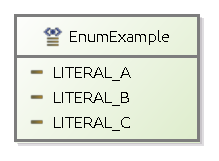
\includegraphics{images/04_transformation_framework/eenum.pdf}
    \caption{Example of an enumeration type in Ecore notation}
    \label{fig:transformation_framework:enumeration_example}
\end{figure}

For example, consider an enumeration type in Ecore, \texttt{EnumExample}, given in \cref{fig:transformation_framework:enumeration_example}. GROOVE has no direct way to express enumerations. However, we can use different encodings to express the enumeration type indirectly. One of such encodings would be to create an abstract node type for the enumeration type and then create a separate node type for each of the values corresponding to the enumeration type. Each of these node types then inherits from the abstract enumeration node type created earlier. An example of this specific encoding is given in \cref{fig:transformation_framework:enumeration_example_groove_encoding_types}. Within an instance graph, each value of an enumeration type is expressed by creating a single node. Each of these nodes is typed by the value node types created earlier. When referencing a value, an edge to the corresponding node can be created.

\begin{figure}
    \centering
    \begin{subfigure}{\textwidth}
        \centering
        % To use this figure in your LaTeX document
% import the package groove/resources/groove2tikz.sty
%
\begin{tikzpicture}[scale=\tikzscale,name prefix=type-]
\node[type_node] (n0) at (4.420, -0.995) {\ml{\textit{\textbf{EnumExample}}}};
\node[type_node] (n1) at (2.040, -0.165) {\ml{\textbf{EnumExample\$LITERAL\_A}}};
\node[type_node] (n2) at (4.420, -0.165) {\ml{\textbf{EnumExample\$LITERAL\_B}}};
\node[type_node] (n3) at (6.800, -0.165) {\ml{\textbf{EnumExample\$LITERAL\_C}}};

\path[subtype_edge] (n1)  --  (n0) ;
\path[subtype_edge](n2.south -| 4.420, -0.995) --  (n0) ;
\path[subtype_edge] (n3)  --  (n0) ;
\end{tikzpicture}

        \caption{GROOVE type graph}
        \label{fig:transformation_framework:enumeration_example_groove_encoding_types:type}
    \end{subfigure}
    \par\medskip
    \begin{subfigure}{\textwidth}
        \centering
        % To use this figure in your LaTeX document
% import the package groove/resources/groove2tikz.sty
%
\begin{tikzpicture}[scale=\tikzscale,name prefix=start-]
\node[basic_node] (n0) at (4.120, -0.170) {\ml{\textbf{EnumExample\$LITERAL\_B}}};
\node[basic_node] (n1) at (6.900, -0.170) {\ml{\textbf{EnumExample\$LITERAL\_C}}};
\node[basic_node] (n2) at (1.340, -0.170) {\ml{\textbf{EnumExample\$LITERAL\_A}}};

\end{tikzpicture}

        \caption{GROOVE instance graph}
        \label{fig:transformation_framework:enumeration_example_groove_encoding_types:instance}
    \end{subfigure}
    \caption{Encoding of the \texttt{EnumExample} enumeration type as different nodes types}
    \label{fig:transformation_framework:enumeration_example_groove_encoding_types}
\end{figure}

Another possible encoding uses flags in GROOVE. In that case, a single node type is created for the enumeration type. This node type gets multiple flags, one for each possible enumeration value. An example of this is shown in \cref{fig:ecore_encodings:enumeration_example_groove_encoding_flags:type}. Within an instance graph, a node is created for each value of the enumeration type. Each of these nodes is typed by the enumeration node type and has a single flag corresponding to the value. An example of these instances is given in \cref{fig:ecore_encodings:enumeration_example_groove_encoding_flags:instance}. This way, each node expresses one value of the enumeration type. When referencing an enumeration value, an edge to the corresponding node can be created.

\begin{figure}
    \centering
    \begin{subfigure}{\textwidth}
        \centering
        % To use this figure in your LaTeX document
% import the package groove/resources/groove2tikz.sty
%
\begin{tikzpicture}[scale=\tikzscale,name prefix=type-]
\node[type_node] (n0) at (0.620, -0.420) {\ml{\textbf{EnumExample}\\\textit{LITERAL\_A}\\\textit{LITERAL\_B}\\\textit{LITERAL\_C}}};

\end{tikzpicture}

        \caption{GROOVE type graph}
        \label{fig:ecore_encodings:enumeration_example_groove_encoding_flags:type}
    \end{subfigure}
    \par\medskip
    \begin{subfigure}{\textwidth}
        \centering
        % To use this figure in your LaTeX document
% import the package groove/resources/groove2tikz.sty
%
\begin{tikzpicture}[scale=\tikzscale,name prefix=start-]
\node[basic_node] (n0) at (1.020, -0.250) {\ml{\textbf{EnumExample}\\\textit{LITERAL\_A}}};
\node[basic_node] (n1) at (2.860, -0.250) {\ml{\textbf{EnumExample}\\\textit{LITERAL\_B}}};
\node[basic_node] (n2) at (4.700, -0.250) {\ml{\textbf{EnumExample}\\\textit{LITERAL\_C}}};

\end{tikzpicture}

        \caption{GROOVE instance graph}
        \label{fig:ecore_encodings:enumeration_example_groove_encoding_flags:instance}
    \end{subfigure}
    \caption{Encoding of the \texttt{EnumExample} enumeration type as one type with multiple flags}
    \label{fig:ecore_encodings:enumeration_example_groove_encoding_flags}
\end{figure}

As the previous examples have shown, creating encodings allows for expressing elements that are unique to Ecore in GROOVE. Moreover, each of these elements might correspond to multiple encodings. The examples for enumeration types presented earlier are non-exhaustive. There are more encodings for enumeration types possible. In other words, there is no single encoding for each element. The choice between different encodings depends on the user, as each encoding might have its advantages and disadvantages.
\section{Structure}
\label{sec:transformation_framework:structure}

Creating a transformation function between Ecore models and GROOVE graphs is a difficult task because there are infinitely many possible transformations that vary in complexity. Complexity in these transformation functions is created by the validity constraints of Ecore models and GROOVE graphs. Another factor that adds complexity is the possibility to mix encodings. For example, a transformation function might encode enumeration type \texttt{A} different from enumeration type \texttt{B}.

The transformation framework presented in this chapter deals with the complexity by providing a structure for building transformation functions out of smaller building blocks. The framework starts with a trivial transformation (the transformation between an empty model and an empty graph). It then adds elements to this transformation, such that we build the model and graph iteratively. When applying each building block, the transformation function is extended while preserving its correctness. Furthermore, the framework ensures that when applying each building block, the correctness of both the model and graph is preserved.

\begin{figure}[H]
    \centering
    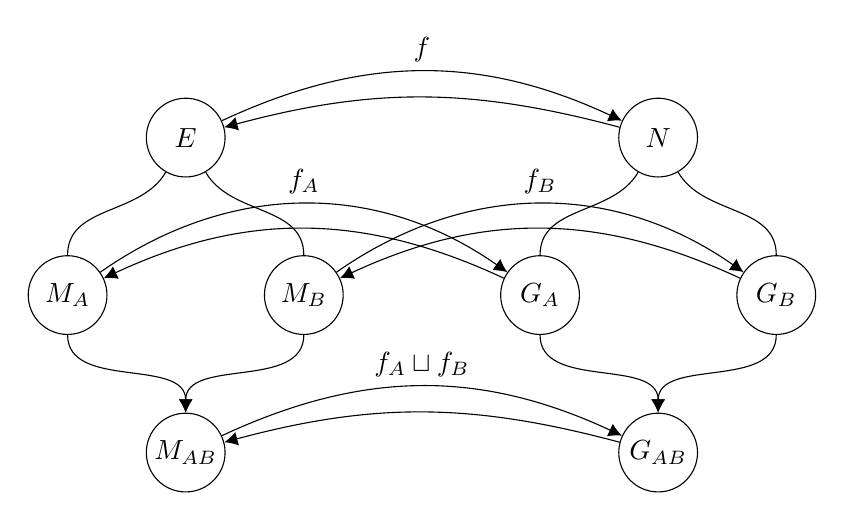
\begin{tikzpicture} 
    \path
    (-3,4) node[circle,draw,minimum size=10mm,inner sep=0pt](ME) {$E$}
    (-4.5,2) node[circle,draw,minimum size=10mm,inner sep=0pt](MA) {$M_A$}
    (-1.5,2) node[circle,draw,minimum size=10mm,inner sep=0pt](MB) {$M_B$}
    (-3,0) node[circle,draw,minimum size=10mm,inner sep=0pt](MAB) {$M_{AB}$}
    
    (3,4) node[circle,draw,minimum size=10mm,inner sep=0pt](GN) {$N$}
    (1.5,2) node[circle,draw,minimum size=10mm,inner sep=0pt](GA) {$G_A$}
    (4.5,2) node[circle,draw,minimum size=10mm,inner sep=0pt](GB) {$G_B$}
    (3,0) node[circle,draw,minimum size=10mm,inner sep=0pt](GAB) {$G_{AB}$};
    
    \path[]		
    (ME) [-, black, out=240, in=90] edge node[above] {} (MA)
    (ME) [-, black, out=300, in=90] edge node[above] {} (MB)
    
    (MA) [-{Latex[width=5]}, black, out=270, in=90] edge node[above] {} (MAB)
    (MB) [-{Latex[width=5]}, black, out=270, in=90] edge node[above] {} (MAB)
    
    (GN) [-, black, out=240, in=90] edge node[above] {} (GA)
    (GN) [-, black, out=300, in=90] edge node[above] {} (GB)
    
    (GA) [-{Latex[width=5]}, black, out=270, in=90] edge node[above] {} (GAB)
    (GB) [-{Latex[width=5]}, black, out=270, in=90] edge node[above] {} (GAB)
    
    (ME) [-{Latex[width=5]}, black, out=25, in=155] edge node[above] {$f$} (GN)
    (GN) [-{Latex[width=5]}, black, out=165, in=15] edge node[above] {} (ME)
    
    (MA) [-{Latex[width=5]}, black, out=35, in=145] edge node[above] {$f_A$} (GA)
    (GA) [-{Latex[width=5]}, black, out=155, in=25] edge node[above] {} (MA)
    
    (MB) [-{Latex[width=5]}, black, out=35, in=145] edge node[above] {$f_B$} (GB)
    (GB) [-{Latex[width=5]}, black, out=155, in=25] edge node[above] {} (MB)
    
    (MAB) [-{Latex[width=5]}, black, out=25, in=155] edge node[above] {$f_{A} \sqcup f_{B}$} (GAB)
    (GAB) [-{Latex[width=5]}, black, out=165, in=15] edge node[above] {} (MAB)
    ;
    \end{tikzpicture}
    \caption{General structure for building a transformation function}
    \label{fig:transformation_framework:general_structure}
\end{figure}

In order for the framework to guarantee these properties, the smaller building blocks are applied in a general structure. A visualisation of this structure is given in \cref{fig:transformation_framework:general_structure}. The structure assumes that we have a partially build model $M_A$, which is valid and corresponds to a valid graph $G_A$ under a certain bijective transformation function $f_A$. In other words, $f_A$ transforms model $M_A$ to graph $G_A$ and the inverse of $f_A$ transforms graph $G_A$ to model $M_A$.

The next step is to add a building block. This building block is represented by valid model $M_B$, which corresponds to a valid graph $G_B$ under a specific bijective transformation function $f_B$. Furthermore, we assume that $M_A$ and $M_B$ are entirely distinct except for some set of elements $E$, which are the only shared elements among the models $M_A$ and $M_B$. In the same way, we assume that graphs $G_A$ and $G_B$ are entirely distinct except for a set of nodes $N$, which are the only shared nodes between graphs $G_A$ and $G_B$. Finally, there also exists a specific bijective transformation function $f$, which transforms the set of elements $E$ to the set of nodes $N$ and vice-versa.

Within the framework, we will present a way to merge models $M_A$ and $M_B$ into a model $M_{AB}$, while preserving validity. We also present a way to merge graphs $G_A$ and $G_B$ intro graph $G_{AB}$, again while preserving validity. Then we present a way to merge two transformation functions $f_A$ and $f_B$ in order to create a transformation function $f_{A} \sqcup f_{B}$, which transforms the combined model $M_{AB}$ to the combined graph $G_{AB}$. By performing these operations, a larger transformation function is created which can transform the larger model $M_{AB}$ to the larger graph $G_{AB}$. Since $M_{AB}$ and $G_{AB}$ are valid and $f_{A} \sqcup f_{B}$ is a bijective transformation function between model $M_{AB}$ and graph $G_{AB}$, it is possible to reuse them as the next $M_{A}$, $G_{A}$ and $f_{A}$ in the model and add another building block. This way, complex model structures and transformation functions are created iteratively while each step in the process maintains a formal proof.

In the following sections, the explained structure is applied to type models and type graphs, and then also to instance models and instance graphs. These sections also discuss the necessary definitions and proofs needed to apply the framework.
\section{Type models and type graphs}
\label{sec:transformation_framework:type_models_and_type_graphs}

In this section, the proposed framework structure is applied to type models and type graphs. First, the general structure and its requirements are discussed. Then the required definitions and theorems are given.

\begin{figure}
    \centering
    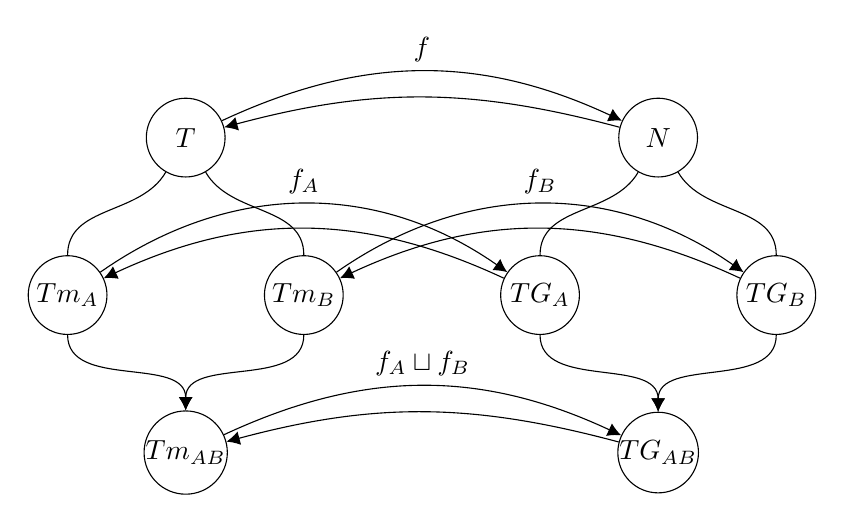
\begin{tikzpicture} 
    \path
    (-3,4) node[circle,draw,minimum size=10mm,inner sep=0pt](ME) {$T$}
    (-4.5,2) node[circle,draw,minimum size=10mm,inner sep=0pt](MA) {$Tm_A$}
    (-1.5,2) node[circle,draw,minimum size=10mm,inner sep=0pt](MB) {$Tm_B$}
    (-3,0) node[circle,draw,minimum size=10mm,inner sep=0pt](MAB) {$Tm_{AB}$}
    
    (3,4) node[circle,draw,minimum size=10mm,inner sep=0pt](GN) {$N$}
    (1.5,2) node[circle,draw,minimum size=10mm,inner sep=0pt](GA) {$TG_A$}
    (4.5,2) node[circle,draw,minimum size=10mm,inner sep=0pt](GB) {$TG_B$}
    (3,0) node[circle,draw,minimum size=10mm,inner sep=0pt](GAB) {$TG_{AB}$};
    
    \path[]		
    (ME) [-, black, out=240, in=90] edge node[above] {} (MA)
    (ME) [-, black, out=300, in=90] edge node[above] {} (MB)
    
    (MA) [-{Latex[width=5]}, black, out=270, in=90] edge node[above] {} (MAB)
    (MB) [-{Latex[width=5]}, black, out=270, in=90] edge node[above] {} (MAB)
    
    (GN) [-, black, out=240, in=90] edge node[above] {} (GA)
    (GN) [-, black, out=300, in=90] edge node[above] {} (GB)
    
    (GA) [-{Latex[width=5]}, black, out=270, in=90] edge node[above] {} (GAB)
    (GB) [-{Latex[width=5]}, black, out=270, in=90] edge node[above] {} (GAB)
    
    (ME) [-{Latex[width=5]}, black, out=25, in=155] edge node[above] {$f$} (GN)
    (GN) [-{Latex[width=5]}, black, out=165, in=15] edge node[above] {} (ME)
    
    (MA) [-{Latex[width=5]}, black, out=35, in=145] edge node[above] {$f_A$} (GA)
    (GA) [-{Latex[width=5]}, black, out=155, in=25] edge node[above] {} (MA)
    
    (MB) [-{Latex[width=5]}, black, out=35, in=145] edge node[above] {$f_B$} (GB)
    (GB) [-{Latex[width=5]}, black, out=155, in=25] edge node[above] {} (MB)
    
    (MAB) [-{Latex[width=5]}, black, out=25, in=155] edge node[above] {$f_{A} \sqcup f_{B}$} (GAB)
    (GAB) [-{Latex[width=5]}, black, out=165, in=15] edge node[above] {} (MAB)
    ;
    \end{tikzpicture}
    \caption{Structure for transforming between type models and type graphs}
    \label{fig:transformation_framework:type_models_and_type_graphs:structure_type_models_graphs}
\end{figure}

\cref{fig:transformation_framework:type_models_and_type_graphs:structure_type_models_graphs} shows an alternation of the structure proposed in \cref{sec:transformation_framework:structure} applied to type models and type graphs. As before, type model $Tm_A$ represents the partially build model which corresponds to type graph $TG_A$ under the transformation function $f_A$. Type model $Tm_B$ represents the next building block to add to this model. It corresponds to type graph $TG_B$ under the bijective transformation function $f_B$.

Type models $Tm_A$ and $Tm_B$ are entirely distinct except for a set types $T$, which means $T \subseteq Type_{Tm_A} \land T \subseteq Type_{Tm_B}$. In a similar way, type graphs $TG_A$ and $TG_B$ are entirely distinct except for a set of node types $N$, so $N \subseteq NT_{TG_A} \land N \subseteq NT_{TG_B}$.

Type models $Tm_A$ and $Tm_B$ are combined into type model $Tm_{AB}$ using \cref{defin:transformation_framework:type_models_and_type_graphs:combining_type_models:combine}. In a similar way type graphs $TG_A$ and $TG_B$ are combined into type graph $TG_{AB}$ using \cref{defin:transformation_framework:type_models_and_type_graphs:combining_type_graphs:combine}. \cref{defin:transformation_framework:type_models_and_type_graphs:combining_type_models:tmod_combine_merge_correct} and \cref{defin:transformation_framework:type_models_and_type_graphs:combining_type_graphs:tg_combine_merge_correct} respectively show that $Tm_{AB}$ and $TG_{AB}$ are valid. Then \cref{defin:transformation_framework:type_models_and_type_graphs:combining_transformation_functions:combination_transformation_function_type_model_type_graph} and \cref{defin:transformation_framework:type_models_and_type_graphs:combining_transformation_functions:combination_transformation_function_type_graph_type_model} can be used to merge the transformation functions $f_A$ and $f_B$ into $f_{A} \sqcup f_{B}$, where \cref{defin:transformation_framework:type_models_and_type_graphs:combining_transformation_functions:tg_combine_mapping_correct} and \cref{defin:transformation_framework:type_models_and_type_graphs:combining_transformation_functions:tg_combine_mapping_function_correct} show that $f_{A} \sqcup f_{B}$ is again a valid transformation function transforming $Tm_{AB}$ to $TG_{AB}$. Similarly, \cref{defin:transformation_framework:type_models_and_type_graphs:combining_transformation_functions:tmod_combine_mapping_correct} and \cref{defin:transformation_framework:type_models_and_type_graphs:combining_transformation_functions:tmod_combine_mapping_function_correct} show that the inverse function of $f_{A} \sqcup f_{B}$ is again a valid transformation function transforming $TG_{AB}$ to $Tm_{AB}$.

\subsection{Combining type models}
\label{subsec:transformation_framework:type_models_and_type_graphs:combining_type_models}

The structure of \cref{fig:transformation_framework:type_models_and_type_graphs:structure_type_models_graphs} shows that the type models $Tm_A$ and $Tm_B$ are combined into one type model $Tm_{AB}$. This section provides the definition of this combination and its corresponding theorems. Please note that the definitions presented here are as generic as possible, and do not actively take into account that $Tm_{A}$ and $Tm_{B}$ are mostly distinct. This bit of information is added later as part of a theorem and proof.

\begin{defin}[Combination function on type models]
\label{defin:transformation_framework:type_models_and_type_graphs:combining_type_models:combine}
$\mathrm{combine}$ is a binary function on two type models which combines two type models into one type model. It is defined as follows:
\begin{align*}
\mathrm{combine}(Tm_A, Tm_B) = \langle&
Class = Class_{Tm_A} \cup Class_{Tm_B} \\&
Enum = Enum_{Tm_A} \cup Enum_{Tm_B} \\&
UserDataType = UserDataType_{Tm_A} \cup UserDataType_{Tm_B} \\&
Field = Field_{Tm_A} \cup Field_{Tm_B} \\&
\mathrm{FieldSig} = \mathrm{fieldsig\_\!combine}(Tm_A, Tm_B) \\&
EnumValue = EnumValue_{Tm_A} \cup EnumValue_{Tm_B} \\&
Inh = Inh_{Tm_A} \cup Inh_{Tm_B} \\&
Prop = \mathrm{prop\_\!combine}(Tm_A, Tm_B) \\&
Constant = Constant_{Tm_A} \cup Constant_{Tm_B} \\&
\mathrm{ConstType} = \mathrm{consttype\_\!combine}(Tm_A, Tm_B)\rangle
\end{align*}

In which $\mathrm{fieldsig\_\!combine}$ is given as part of \cref{defin:transformation_framework:type_models_and_type_graphs:combining_type_models:fieldsig_combine}, $\mathrm{prop\_\!combine}$ as part of \cref{defin:transformation_framework:type_models_and_type_graphs:combining_type_models:prop_combine} and $\mathrm{consttype\_\!combine}$ as part of \cref{defin:transformation_framework:type_models_and_type_graphs:combining_type_models:consttype_combine}.
\isabellelref{tmod_combine}{Ecore.Type_Model_Combination}
\end{defin}

The combination of two type models is rather simple in its definition, at least for all the sets defined as part of a type model. Intuitively, the definition makes sense. To combine two type models, we need the types from both type models, so we merge the classes, enumerations types, enumeration values and user-defined data types. The constants should also be preserved, so these are merged too. To preserve all attributes and relations, we merge the set of fields and the inheritance relation as well.

Merging the different functions is done by using a new function. First, the combination of field signatures will be discussed.

\begin{defin}[Combination function for field signatures]
\label{defin:transformation_framework:type_models_and_type_graphs:combining_type_models:fieldsig_combine}
$\mathrm{fieldsig\_\!combine}$ is a partial function on two type models which returns a new function $Field_{Tm_{AB}} \Rightarrow (Type_{Tm_{AB}} \times \mathbb{M})$. It is defined as follows:
\begin{multline*}
    \mathrm{fieldsig\_\!combine}(Tm_{A}, Tm_{B}, f) = \\
        \begin{cases}
        s & \mathrm{if } f \in Field_{Tm_A} \cap Field_{Tm_B} \land \mathrm{type}_{Tm_A}(f) = \mathrm{type}_{Tm_B}(f) \\
        \mathrm{FieldSig}_{Tm_A}(f) & \mathrm{if } f \in Field_{Tm_A} \setminus Field_{Tm_B} \\
        \mathrm{FieldSig}_{Tm_B}(f) & \mathrm{if } f \in Field_{Tm_B} \setminus Field_{Tm_A}
    \end{cases}
\end{multline*}
where
\begin{equation*}
\begin{split}
    s = \bigg(\mathrm{type}_{Tm_A}(f), \Big(\max\left(\mathrm{lower}(\mathrm{FieldSig}_{Tm_A}(f)), \mathrm{lower}(\mathrm{FieldSig}_{Tm_B}(f))\right) ..\\ \min\left(\mathrm{upper}(\mathrm{FieldSig}_{Tm_A}(f)), \mathrm{upper}(\mathrm{FieldSig}_{Tm_B}(f))\right)\Big)\bigg)
\end{split}
\end{equation*}
\isabellelref{tmod_combine_fieldsig}{Ecore.Type_Model_Combination}
\end{defin}

Although the above definition looks quite complex, the intuition behind it is straightforward. For a field that only occurs in type model $Tm_A$, the field signature over from $Tm_A$ is copied. For a field that only occurs in $Tm_B$, the field signature from $Tm_B$ is copied. In the case that a field occurs in both $Tm_A$ and $Tm_B$, it should be the case that the type of the fields is the same. If this is indeed the case, the field type is copied, and a new multiplicity is created. This multiplicity takes the maximum of the lower bounds of the field in $Tm_A$ and $Tm_B$ as new lower bound, and the minimum of the upper bounds of the field in $Tm_A$ and $Tm_B$ as new upper bound.

\begin{figure}
    \centering
    \begin{subfigure}{0.45\textwidth}
        \centering
        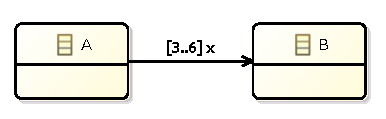
\includegraphics{images/04_transformation_framework/type_models_combination/fieldsig_combine_tmod1.pdf}
        \caption{First type model $Tm_A$}
        \label{fig:transformation_framework:type_models_and_type_graphs:combining_type_models:fieldsig_combine_tmod1}
    \end{subfigure}
    \begin{subfigure}{0.45\textwidth}
        \centering
        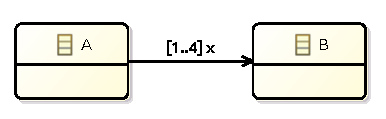
\includegraphics{images/04_transformation_framework/type_models_combination/fieldsig_combine_tmod2.pdf}
        \caption{Second type model $Tm_A$}
        \label{fig:transformation_framework:type_models_and_type_graphs:combining_type_models:fieldsig_combine_tmod2}
    \end{subfigure}
    \par\medskip
    \begin{subfigure}{\textwidth}
        \centering
        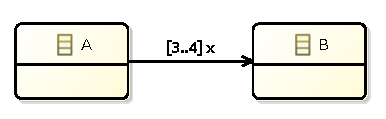
\includegraphics{images/04_transformation_framework/type_models_combination/fieldsig_combine_tmod12.pdf}
        \caption{Combined type model $Tm_{AB}$}
        \label{fig:transformation_framework:type_models_and_type_graphs:combining_type_models:fieldsig_combine_tmod12}
    \end{subfigure}
    \caption{Combination of field signatures when field is present in both type models}
    \label{fig:transformation_framework:type_models_and_type_graphs:combining_type_models:fieldsig_combine}
\end{figure}

An example of the combination of two field signatures in the case of a field being present in both $Tm_A$ and $Tm_B$ is given in \cref{fig:transformation_framework:type_models_and_type_graphs:combining_type_models:fieldsig_combine}. It is possible to combine the field $\type{x}$, since in both $Tm_A$ and $Tm_B$ field $\type{x}$ references class type $\type{B}$. The multiplicity for both field signatures is different and is combined as defined. The maximum of the lower bounds is taken, which results in $\max(3, 1) = 3$. Furthermore, the minimum of the upper bounds is taken, which results in $\min(6, 4) = 4$. Therefore the multiplicity of $\type{x}$ in $Tm_{AB}$ will become $3..4$.

Besides a function for field signatures, a type model also defines a function for constant types. The combination of constant types is discussed in the next definition.

\begin{defin}[Combination function for constant types]
\label{defin:transformation_framework:type_models_and_type_graphs:combining_type_models:consttype_combine}
$\mathrm{consttype\_\!combine}$ is a partial function on two type models which returns a new function \\$Constant_{Tm_{AB}} \Rightarrow Type_{Tm_{AB}}$. It is defined as follows:
\begin{multline*}
    \mathrm{consttype\_\!combine}(Tm_{A}, Tm_{B}, c) = \\
        \begin{cases}
        \mathrm{ConstType}_{Tm_A}(c) & \mathrm{if}\ c \in Constant_{Tm_A} \cap Constant_{Tm_B} \land \mathrm{ConstType}_{Tm_A}(c) = \mathrm{ConstType}_{Tm_B}(c) \\
        \mathrm{ConstType}_{Tm_A}(c) & \mathrm{if}\ c \in Constant_{Tm_A} \setminus Constant_{Tm_B} \\
        \mathrm{ConstType}_{Tm_B}(c) & \mathrm{if}\ c \in Constant_{Tm_B} \setminus Constant_{Tm_A}
    \end{cases}
\end{multline*}
\isabellelref{tmod_combine_const_type}{Ecore.Type_Model_Combination}
\end{defin}

The definition of the combination of constant types is similar to the combination of field signatures. The combination of constant types is less complicated because there is no notion of multiplicities involved. By definition, if a constant only occurs in $Tm_{A}$, the constant type of $Tm_{A}$ is copied. For constants that only occur in $Tm_{B}$, the constant type of $Tm_{B}$ is copied. In case that a constant occurs in both $Tm_{A}$ and $Tm_{B}$, the constant is copied if the constant types for that constant are the same in both $Tm_{A}$ and $Tm_{B}$.

The last definition that remains to be given is the definition of combining the set of properties. The set of properties cannot be united by merely taking the union of $Prop_{Tm_A}$ and $Prop_{Tm_B}$ since this might invalidate the satisfaction of these properties on the level of an instance graph. Instead, the inductive set $\mathrm{prop\_\!combine}$ is defined to specify under which circumstances a property can be combined.

\begin{defin}[Combination of model properties]
\label{defin:transformation_framework:type_models_and_type_graphs:combining_type_models:prop_combine}
$\mathrm{prop\_\!combine}(Tm_A, Tm_B)$ is defined as a subset of $Prop_{Tm_A} \cup Prop_{Tm_B}$. The contents of the set are then defined as follows:

For $\type{abstract}$ properties:
\begin{mathpar}
    \inferrule{[ \type{abstract}, c ] \in Prop_{Tm_A} \\ c \not\in Class_{Tm_B}}{[ \type{abstract}, c ] \in \mathrm{prop\_\!combine}(Tm_A, Tm_B)}
    \and
    \inferrule{[ \type{abstract}, c ] \in Prop_{Tm_B} \\ c \not\in Class_{Tm_A}}{[ \type{abstract}, c ] \in \mathrm{prop\_\!combine}(Tm_A, Tm_B)}
    \and
    \inferrule{[ \type{abstract}, c ] \in Prop_{Tm_A} \\ [ \type{abstract}, c ] \in Prop_{Tm_B}}{[ \type{abstract}, c ] \in \mathrm{prop\_\!combine}(Tm_A, Tm_B)}
\end{mathpar}

For $\type{containment}$ properties:
\begin{mathpar}
    \inferrule{[ \type{containment}, r ]\in Prop_{Tm_A}}{[ \type{containment}, r ]\in \mathrm{prop\_\!combine}(Tm_A, Tm_B)}
    \and
    \inferrule{[ \type{containment}, r ]\in Prop_{Tm_B}}{[ \type{containment}, r ]\in \mathrm{prop\_\!combine}(Tm_A, Tm_B)}
\end{mathpar}

For $\type{defaultValue}$ properties:
\begin{mathpar}
    \inferrule{[ \type{defaultValue}, f, v ]\in Prop_{Tm_A} \\ f \not\in Field_{Tm_B}}{[ \type{defaultValue}, f, v ]\in \mathrm{prop\_\!combine}(Tm_A, Tm_B)}
    \and
    \inferrule{[ \type{defaultValue}, f, v ]\in Prop_{Tm_B} \\ f \not\in Field_{Tm_A}}{[ \type{defaultValue}, f, v ]\in \mathrm{prop\_\!combine}(Tm_A, Tm_B)}
    \and
    \inferrule{[ \type{defaultValue}, f, v ]\in Prop_{Tm_A} \\ [ \type{defaultValue}, f, v ]\in Prop_{Tm_B}}{[ \type{defaultValue}, f, v ]\in \mathrm{prop\_\!combine}(Tm_A, Tm_B)}
\end{mathpar}

For $\type{identity}$ properties:
\begin{mathpar}
    \inferrule{[ \type{identity}, c, A ]\in Prop_{Tm_A} \\ c \not\in Class_{Tm_B}}{[ \type{identity}, c, A ]\in \mathrm{prop\_\!combine}(Tm_A, Tm_B)}
    \and
    \inferrule{[ \type{identity}, c, A ]\in Prop_{Tm_B} \\ c \not\in Class_{Tm_A}}{[ \type{identity}, c, A ]\in \mathrm{prop\_\!combine}(Tm_A, Tm_B)}
    \and
    \inferrule{[ \type{identity}, c, A ]\in Prop_{Tm_A} \\ [ \type{identity}, c, A ]\in Prop_{Tm_B}}{[ \type{identity}, c, A ]\in \mathrm{prop\_\!combine}(Tm_A, Tm_B)}
\end{mathpar}

For $\type{keyset}$ properties:
\begin{mathpar}
    \inferrule{[ \type{keyset}, r, A ]\in Prop_{Tm_A} \\ r \not\in Field_{Tm_B}}{[ \type{keyset}, r, A ]\in \mathrm{prop\_\!combine}(Tm_A, Tm_B)}
    \and
    \inferrule{[ \type{keyset}, r, A ]\in Prop_{Tm_B} \\ r \not\in Field_{Tm_A}}{[ \type{keyset}, r, A ]\in \mathrm{prop\_\!combine}(Tm_A, Tm_B)}
    \and
    \inferrule{[ \type{keyset}, r, A ]\in Prop_{Tm_A} \\ [ \type{keyset}, r, A ]\in Prop_{Tm_B}}{[ \type{keyset}, r, A ]\in \mathrm{prop\_\!combine}(Tm_A, Tm_B)}
\end{mathpar}

For $\type{opposite}$ properties:
\begin{mathpar}
    \inferrule{[ \type{opposite}, r1, r2 ]\in Prop_{Tm_A} \\ r1 \not\in Field_{Tm_B} \\ r2 \not\in Field_{Tm_B}}{[ \type{opposite}, r1, r2 ]\in \mathrm{prop\_\!combine}(Tm_A, Tm_B)}
    \and
    \inferrule{[ \type{opposite}, r1, r2 ]\in Prop_{Tm_B} \\ r1 \not\in Field_{Tm_A} \\ r2 \not\in Field_{Tm_A}}{[ \type{opposite}, r1, r2 ]\in \mathrm{prop\_\!combine}(Tm_A, Tm_B)}
    \and
    \inferrule{[ \type{opposite}, r1, r2 ]\in Prop_{Tm_A} \\ [ \type{opposite}, r1, r2 ]\in Prop_{Tm_B}}{[ \type{opposite}, r1, r2 ]\in \mathrm{prop\_\!combine}(Tm_A, Tm_B)}
\end{mathpar}

For $\type{readonly}$ properties:
\begin{mathpar}
    \inferrule{[ \type{readonly}, f ] \in Prop_{Tm_A} \\ f \not\in Field_{Tm_B}}{[ \type{readonly}, f ] \in \mathrm{prop\_\!combine}(Tm_A, Tm_B)}
    \and
    \inferrule{[ \type{readonly}, f ] \in Prop_{Tm_B} \\ f \not\in Field_{Tm_A}}{[ \type{readonly}, f ] \in \mathrm{prop\_\!combine}(Tm_A, Tm_B)}
    \and
    \inferrule{[ \type{readonly}, f ] \in Prop_{Tm_A} \\ [ \type{readonly}, f ] \in Prop_{Tm_B}}{[ \type{readonly}, f ] \in \mathrm{prop\_\!combine}(Tm_A, Tm_B)}
\end{mathpar}
\isabellelref{tmod_combine_prop}{Ecore.Type_Model_Combination}
\end{defin}

As can be seen from the definition of $\mathrm{prop\_\!combine}(Tm_A, Tm_B)$, properties are only copied under specific circumstances. For $\type{abstract}$ properties, it holds that a class is only abstract in the combination of $Tm_A$ and $Tm_B$ if the class is abstract in both $Tm_A$ and $Tm_B$ or if the class is abstract in one of them, and the class does not occur in the other. Intuitively, this makes sense for correctness. If a class is abstract in both type models, there will not be instances of that class in any of the combined instance models type by those type models. The same holds if the class only occurs in one of the type models, as an instance model cannot contain an instance of a class that is not present in its type model.

For the containment property, it holds that the containment property is always copied over. There are no other conditions here. If there is a containment property in $Prop_{Tm_A} \cup Prop_{Tm_B}$ it will also be in the combination of $Tm_A$ and $Tm_B$.

A default value property is copied over from one of the type models if the other type model does not have the corresponding field defined. Furthermore, a default value may be in the combination of properties of $Tm_A$ and $Tm_B$ if the field occurs in both, and both have the same constant set as the default value for the field. Intuitively, this last requirement makes sense. If we set a default value for a field within a type model, it should not change after combining the type model with another type model, as instance models might depend on the default value set for that field.

Identity properties follow a similar pattern to default value properties. An identity is copied over from one of the type models if the corresponding class is not defined in the other type model. Furthermore, an identity can be preserved if it is set for the same class and attributes in both type models. Again, intuitively, this is the desired solution. If a type model has a class of which a set of attributes can uniquely define the instances, then this should also be the case after the combination with another type model. Merging two sets of attributes might have preserved the identity property as well, but this would be a questionable decision from a practical standpoint, as this means that the identity of instances changes, which makes no sense in real-world scenarios.

The argumentation for identity properties also holds for keyset properties. Therefore these follow a similar pattern, in which the keyset properties of a type model are only copied if the corresponding field does not occur in the other type model, or if the keyset property for a field occurs with the same attributes in both type models.

The opposite property is preserved if it occurs in a type model, but the other type model does not define both of the corresponding fields. Alternatively, the property is preserved if it occurs in both type models with the same fields. All different ways to combine an opposite property would result in an invalid type model according to \cref{defin:formalisations:ecore_formalisation:type_models:type_model_consistency}, which is undesired.

The read-only properties follow a similar pattern to the abstract properties. If a field is read-only in both type models, then it is read-only in the combination. Furthermore, if a field is read-only in one of the type models and the field is not defined in the other type model, then the read-only property can be copied too.

\begin{figure}
    \centering
    \begin{subfigure}{\textwidth}
        \centering
        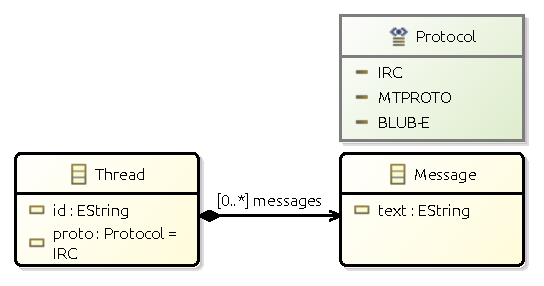
\includegraphics{images/04_transformation_framework/type_models_combination/chat_partial2.pdf}
        \caption{The chat application model $Tm_{Chat}$}
        \label{fig:transformation_framework:type_models_and_type_graphs:combining_type_models:combine_example_tmod1}
    \end{subfigure}
    \par\medskip
    \begin{subfigure}{\textwidth}
        \centering
        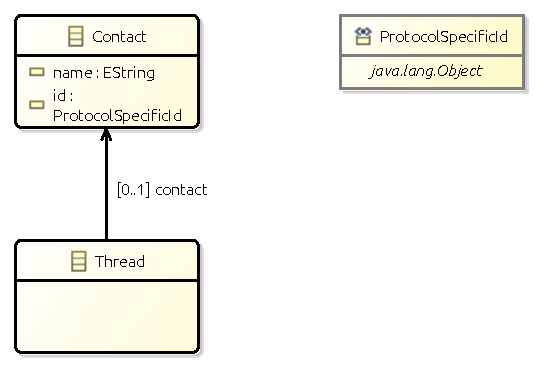
\includegraphics{images/04_transformation_framework/type_models_combination/chat_partial1.pdf}
        \caption{The contact extension model $Tm_{Extension}$}
        \label{fig:transformation_framework:type_models_and_type_graphs:combining_type_models:combine_example_tmod2}
    \end{subfigure}
    \par\medskip
    \begin{subfigure}{\textwidth}
        \centering
        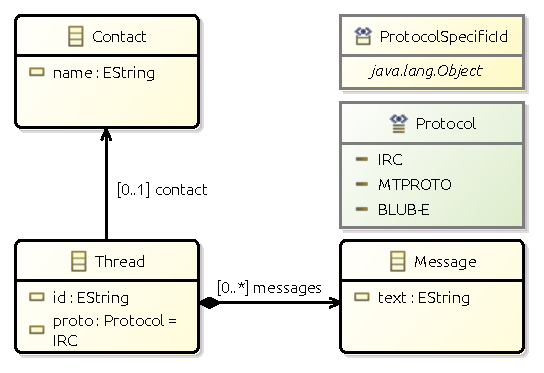
\includegraphics{images/04_transformation_framework/type_models_combination/chat_combined.pdf}
        \caption{The extended chat application model $Tm_{ChatExt}$}
        \label{fig:transformation_framework:type_models_and_type_graphs:combining_type_models:combine_example_tmod12}
    \end{subfigure}
    \caption{Example of the combination of type models}
    \label{fig:transformation_framework:type_models_and_type_graphs:combining_type_models:combine_example}
\end{figure}

With all definitions in place, it is possible to provide a larger example. Suppose the model of a multi-protocol chat application. It consists of $\type{Thread}$s of $\type{Message}$s. Since the application is multi-protocol, each $\type{Thread}$ can use one of the supported $\type{Protocol}$s. The formal definition of the model of such an application could be as follows:

\begin{align*}
Tm_{Chat} =\ &\langle&
Class =\ &\{ \type{.Message}, \type{.Thread} \} \\&&
Enum =\ &\{ \type{.Protocol} \} \\&&
UserDataType =\ &\{\} \\&&
Field =\ &\{
( \type{.Message}, \type{text} ), 
( \type{.Thread}, \type{id} ), 
( \type{.Thread}, \type{messages} ), 
( \type{.Thread}, \type{proto} )\} \\&&
\mathrm{FieldSig} =\ &\big\{
\big( ( \type{.Message}, \type{text} ), ( \type{string}, 1..1 ) \big), \big( ( \type{.Thread}, \type{id} ), ( \type{string}, 1..1 ) \big),\\&&& 
\big( ( \type{.Thread}, \type{messages} ), ( [ \type{seqof}, !\type{.Message} ], 0..\mstar ) \big),\\&&& 
\big( ( \type{.Thread}, \type{proto} ), ( \type{.Protocol}, 1..1 ) \big) \big)
\big\} \\&&
EnumValue =\ &\{
( \type{.Protocol}, \type{IRC} ), 
( \type{.Protocol}, \type{MTPROTO} ), 
( \type{.Protocol}, \type{BLUB\!-\!E} )\} \\&&
Inh =\ &\{\} \\&&
Prop =\ &\big\{
\big( \type{identity}, \type{.Message}, \{( \type{.Thread}, \type{id} )\} \big)
\big\} \\&&
Constant =\ &\{\} \\&&
\mathrm{ConstType} =\ &\{\}
\\&\rangle
\end{align*}

An visual representation of $Tm_{Chat}$ is included as  \cref{fig:transformation_framework:type_models_and_type_graphs:combining_type_models:combine_example_tmod1}. Now, assume a model that represents an extension to this application, adding support for $\type{Contact}$s. Each thread can belong to a $\type{Contact}$. A $\type{Contact}$ has a name and some identifier that is protocol specific. For that identifier, the user-defined data type $\type{ProtocolSpecificId}$ is introduced. This extension could formally be defined as:

\begin{align*}
Tm_{Extension} =\ &\langle&
Class =\ &\{ \type{.Contact}, \type{.Thread} \} \\&&
Enum =\ &\{\} \\&&
UserDataType =\ &\{ \type{.ProtocolSpecificId} \} \\&&
Field =\ &\{
( \type{.Contact}, \type{name} ), 
( \type{.Contact}, \type{id} ), 
( \type{.Thread}, \type{contact} )\} \\&&
\mathrm{FieldSig} =\ &\big\{
\big( ( \type{.Contact}, \type{name} ), ( \type{string}, 1..1 ) \big),\\&&& \big( ( \type{.Contact}, \type{id} ), ( \type{.ProtocolSpecificId}, 1..1 ) \big),\\&&& 
\big( ( \type{.Thread}, \type{contact} ), ( ?\type{.Contact}, 0..1 ) \big) \big)
\big\} \\&&
EnumValue =\ &\{\} \\&&
Inh =\ &\{\} \\&&
Prop =\ &\big\{
\big( \type{identity}, \type{.Contact}, \{( \type{.Contact}, \type{id} )\} \big)
\big\} \\&&
Constant =\ &\{\} \\&&
\mathrm{ConstType} =\ &\{\}
\\&\rangle
\end{align*}

The visual representation of the extension is included as \cref{fig:transformation_framework:type_models_and_type_graphs:combining_type_models:combine_example_tmod2}. Now, using \cref{defin:transformation_framework:type_models_and_type_graphs:combining_type_models:combine}, it is possible to combine these models into one model. This will yield the following model:

\begin{align*}
Tm_{ChatExt} =\ &\langle&
Class =\ &\{ \type{.Contact}, \type{.Message}, \type{.Thread} \} \\&&
Enum =\ &\{ \type{.Protocol} \} \\&&
UserDataType =\ &\{ \type{.ProtocolSpecificId} \} \\&&
Field =\ &\{
( \type{.Contact}, \type{name} ), 
( \type{.Contact}, \type{id} ),
( \type{.Message}, \type{text} ),\\&&&
( \type{.Thread}, \type{contact} ),
( \type{.Thread}, \type{id} ),
( \type{.Thread}, \type{messages} ),\\&&& 
( \type{.Thread}, \type{proto} )\} \\&&
\mathrm{FieldSig} =\ &\big\{
\big( ( \type{.Contact}, \type{name} ), ( \type{string}, 1..1 ) \big),\\&&& \big( ( \type{.Contact}, \type{id} ), ( \type{.ProtocolSpecificId}, 1..1 ) \big),\\&&& 
\big( ( \type{.Message}, \type{text} ), ( \type{string}, 1..1 ) \big),\\&&&
\big( ( \type{.Thread}, \type{contact} ), ( ?\type{.Contact}, 0..1 ) \big) \big),\\&&&
\big( ( \type{.Thread}, \type{id} ), ( \type{string}, 1..1 ) \big),\\&&& 
\big( ( \type{.Thread}, \type{messages} ), ( [ \type{seqof}, !\type{.Message} ], 0..\mstar ) \big),\\&&& 
\big( ( \type{.Thread}, \type{proto} ), ( \type{.Protocol}, 1..1 ) \big) \big)
\big\} \\&&
EnumValue =\ &\{
( \type{.Protocol}, \type{IRC} ), 
( \type{.Protocol}, \type{MTPROTO} ), 
( \type{.Protocol}, \type{BLUB\!-\!E} )\} \\&&
Inh =\ &\{\} \\&&
Prop =\ &\big\{
\big( \type{identity}, \type{.Contact}, \{( \type{.Contact}, \type{id} )\} \big),\\&&&
\big( \type{identity}, \type{.Message}, \{( \type{.Thread}, \type{id} )\} \big)
\big\} \\&&
Constant =\ &\{\} \\&&
\mathrm{ConstType} =\ &\{\}
\\&\rangle
\end{align*}

A visual representation of this combined model is included as \cref{fig:transformation_framework:type_models_and_type_graphs:combining_type_models:combine_example_tmod12}. The example perfectly shows why the combination of type models is useful: It allows for building larger models out of smaller building blocks. This is the exact goal of this definition within the transformation framework.

Although the definitions of the combination of type models are given, no mathematical properties or theorems are defined yet. Some mathematical properties hold for the combination of type models, that will be presented in the following theorems.

\begin{thm}[Commutativity of the combination of type models]
\label{defin:transformation_framework:type_models_and_type_graphs:combining_type_models:tmod_combine_commute}
Assume that $Tm_A$ and $Tm_B$ are type models, then the $\mathrm{combine}$ function is commutative:
\begin{equation*}
    \mathrm{combine}(Tm_A, Tm_B) = \mathrm{combine}(Tm_B, Tm_A)
\end{equation*}
\isabellelref{tmod_combine_commute}{Ecore.Type_Model_Combination}
\end{thm}

\begin{thm}[Associativity of the combination of type models]
\label{defin:transformation_framework:type_models_and_type_graphs:combining_type_models:tmod_combine_assoc}
Assume that $Tm_A$, $Tm_B$ and $Tm_C$ are type models, then the $\mathrm{combine}$ function is associative:
\begin{equation*}
    \mathrm{combine}(\mathrm{combine}(Tm_A, Tm_B), Tm_C) = \mathrm{combine}(Tm_A, \mathrm{combine}(Tm_B, Tm_C))
\end{equation*}
\isabellelref{tmod_combine_assoc}{Ecore.Type_Model_Combination}
\end{thm}

\begin{thm}[Idempotence of the combination of type models]
\label{defin:transformation_framework:type_models_and_type_graphs:combining_type_models:tmod_combine_idemp}
Assume that $Tm_A$ is a type model and that it is consistent in the sense of \cref{defin:formalisations:ecore_formalisation:type_models:type_model_consistency}. Then the following property holds:
\begin{equation*}
    \mathrm{combine}(Tm_A, Tm_A) = Tm_A
\end{equation*}
\isabellelref{tmod_combine_idemp_alt}{Ecore.Type_Model_Combination}
\end{thm}

These properties follow directly from \cref{defin:transformation_framework:type_models_and_type_graphs:combining_type_models:combine}, but the corresponding proofs will not be included here. It should be noted that these properties are indeed proven correct as part of this thesis, and the corresponding proofs are validated within Isabelle.

Besides these properties, the combination of type models also has an identity element. The empty type model represents this identity element, but it needs to be defined first:

\begin{defin}[Empty type model]
\label{defin:transformation_framework:type_models_and_type_graphs:combining_type_models:empty_type_model}
Let $Tm_{\epsilon}$ be the empty type model. $Tm_{\epsilon}$ is defined as:
\begin{align*}
Tm_{\epsilon} = \langle&
Class = \{\} \\&
Enum = \{\} \\&
UserDataType = \{\} \\&
Field = \{\} \\&
\mathrm{FieldSig} = undefined \\&
EnumValue = \{\} \\&
Inh = \{\} \\&
Prop = \{\} \\&
Constant = \{\} \\&
\mathrm{ConstType} = undefined\rangle
\end{align*}
\end{defin}

\begin{thm}[Correctness of the empty type model]
\label{defin:transformation_framework:type_models_and_type_graphs:combining_type_models:tmod_empty_correct}
The empty type model, $Tm_{\epsilon}$, is consistent with respect to
\cref{defin:formalisations:ecore_formalisation:type_models:type_model_consistency}.
\isabellelref{tmod_empty_correct}{Ecore.Type_Model}
\end{thm}

The proof for the correctness of the empty type model is trivial. Still, a validated version of this proof can be found within the Isabelle theories of this thesis.

As mentioned earlier, the empty type model acts as an identity element when combining two type models. The following theorem specifies this behaviour.

\begin{thm}[Identity of the combination of type models]
\label{defin:transformation_framework:type_models_and_type_graphs:combining_type_models:tmod_combine_identity}
Assume that $Tm_A$ is a type model and that it is consistent in the sense of \cref{defin:formalisations:ecore_formalisation:type_models:type_model_consistency}. Then $Tm_{\epsilon}$ acts as an identity element in the combination function:
\begin{equation*}
    \mathrm{combine}(Tm_{\epsilon}, Tm_A) = Tm_A
\end{equation*}
\isabellelref{tmod_combine_identity_alt}{Ecore.Type_Model_Combination}
\end{thm}

Once more, the proof of this theorem follows directly from the definition. Therefore, the corresponding proof will not be included here, but a validated version can be found within the Isabelle theories of this thesis.

A final desired property for the combination of type models is a correctness property. \cref{defin:transformation_framework:type_models_and_type_graphs:combining_type_models:tmod_combine_correct} defines the theorem under which the combination of type models is a consistent type model. Please note that this theorem is a generic theorem, which does not take into account that the type models are mostly distinct.

\begin{thm}[Consistency of the combination of type models]
\label{defin:transformation_framework:type_models_and_type_graphs:combining_type_models:tmod_combine_correct}
Assume that $Tm_A$ and $Tm_B$ are consistent type models in the sense of \cref{defin:formalisations:ecore_formalisation:type_models:type_model_consistency}. Furthermore, assume the following properties:
\begin{itemize}
    \item For all shared fields, the type is the same in both type models: $\forall f \in Field_{Tm_A} \cap Field_{Tm_B}\!: \mathrm{type}_{Tm_A}(f) = \mathrm{type}_{Tm_B}(f)$
    \item For all shared fields, the combination of the multiplicities is a valid multiplicity: $\forall f \in Field_{Tm_A} \cap Field_{Tm_B}\!: \max\big(\mathrm{lower}(\mathrm{FieldSig}_{Tm_A}(f)), \mathrm{lower}(\mathrm{FieldSig}_{Tm_B}(f))\big) .. \min\big(\mathrm{upper}(\mathrm{FieldSig}_{Tm_A}(f)),$\\ $\mathrm{upper}(\mathrm{FieldSig}_{Tm_B}(f))\big) \in \mathbb{M}$
    \item For all shared constants, the constant type is the same in both models: $\forall f \in Constant_{Tm_A} \cap Constant_{Tm_B}\!: \mathrm{ConstType}_{Tm_A}(f) = \mathrm{ConstType}_{Tm_B}(f)$
    \item Identifiers used for a class in $Tm_A$ cannot be used for an enumeration type or user-defined data type in $Tm_B$: $\forall c \in Class_{Tm_A}\!: c \not\in Enum_{Tm_B} \land c \not\in UserDataType_{Tm_B}$.
    \item Identifiers used for a class in $Tm_B$ cannot be used for an enumeration type or user-defined data type in $Tm_A$: $\forall c \in Class_{Tm_B}\!: c \not\in Enum_{Tm_A} \land c \not\in UserDataType_{Tm_A}$.
    \item Identifiers used for an enumeration type in $Tm_A$ cannot be used for a class or user-defined data type in $Tm_B$: $\forall c \in Enum_{Tm_A}\!: c \not\in Class_{Tm_B} \land c \not\in UserDataType_{Tm_B}$.
    \item Identifiers used for an enumeration type in $Tm_B$ cannot be used for a class or user-defined data type in $Tm_A$: $\forall c \in Enum_{Tm_B}\!: c \not\in Class_{Tm_A} \land c \not\in UserDataType_{Tm_A}$.
    \item Identifiers from $Tm_A$ may not be in the namespace of an identifier in $Tm_B$: $\forall x \in Class_{Tm_A} \cup Enum_{Tm_A} \cup UserDataType_{Tm_A}; y \in Class_{Tm_B} \cup Enum_{Tm_B} \cup UserDataType_{Tm_B}\!:$\\$x \text{ not in the namespace of } y$
    \item Identifiers from $Tm_B$ may not be in the namespace of an identifier in $Tm_A$: $\forall x \in Class_{Tm_B} \cup Enum_{Tm_B} \cup UserDataType_{Tm_B}; y \in Class_{Tm_A} \cup Enum_{Tm_A} \cup UserDataType_{Tm_A}\!:$\\$x \text{ not in the namespace of } y$
    \item The transitive closure of the inheritance relation is irreflexive: $(Inh_{Tm_A} \cup Inh_{Tm_B})^+$ is irreflexive
    \item For any superclass with an identity, the identity of the subclasses must be a superset of the identity of the superclass: $\forall c_1\ c_2\ A_1\ A_2\!: [ \type{identity}, c_1, A_1 ] \in \mathrm{prop\_\!combine}(Tm_A, Tm_B) \land [ \type{identity}, c_2, A_2 ] \in \mathrm{prop\_\!combine}(Tm_A, Tm_B) \land c_1 \neq c_2\ \land\ !c_1 \not\sqsubseteq_{Tm_A}\ !c_2\ \land\ !c_1 \not\sqsubseteq_{Tm_B}\ !c_2\ \land\ !c_1 \sqsubseteq_{\mathrm{combine}(Tm_A, Tm_B)}\ !c_2 \implies A \subseteq B$
    \item For all shared fields, if $Tm_{A}$ defines a default value, $Tm_{B}$ should define the same default value, and vice versa: $\forall f \in Field_{Tm_A} \cap Field_{Tm_B}\!: [ \type{defaultValue}, f, v ] \in Prop_{Tm_A} \Longleftrightarrow [ \type{defaultValue}, f, v ] \in Prop_{Tm_B}$.
    \item For all shared classes, if $Tm_{A}$ defines a identity, $Tm_{B}$ should define the same identity, and vice versa: $\forall c \in Class_{Tm_A} \cap Class_{Tm_B}\!: [ \type{identity}, c, A ] \in Prop_{Tm_A} \Longleftrightarrow [ \type{identity}, c, A ] \in Prop_{Tm_B}$.
    \item For all shared fields, if $Tm_{A}$ defines a keyset, $Tm_{B}$ should define the same keyset, and vice versa: $\forall r \in Field_{Tm_A} \cap Field_{Tm_B}\!: [ \type{keyset}, r, A ] \in Prop_{Tm_A} \Longleftrightarrow [ \type{keyset}, r, A ] \in Prop_{Tm_B}$.
    \item For all shared fields, if $Tm_{A}$ defines an opposite property, $Tm_{B}$ should define the same opposite property, and vice versa: $\forall r \in Field_{Tm_A} \cap Field_{Tm_B}\!: [ \type{opposite}, r, r' ] \in Prop_{Tm_A} \Longleftrightarrow [ \type{opposite}, r, r' ] \in Prop_{Tm_B}$
\end{itemize}

Then $\mathrm{combine}(Tm_A, Tm_B)$ is a consistent type model in the sense of \cref{defin:formalisations:ecore_formalisation:type_models:type_model_consistency}
\isabellelref{tmod_combine_correct}{Ecore.Type_Model_Combination}
\end{thm}

\begin{proof}
To proof that $\mathrm{combine}(Tm_A, Tm_B)$ is a consistent type model, it needs to be shown that\\ $\mathrm{combine}(Tm_A, Tm_B)$ gives rise to a valid structure for a type model and that \cref{defin:formalisations:ecore_formalisation:type_models:type_model_consistency} holds. For readability, define $Tm_{AB}$ to be $\mathrm{combine}(Tm_A, Tm_B)$.

\emph{Structural properties}
\begin{itemize}
    \item All elements of $Class_{Tm_{AB}}$ are elements of $Id$.
    
    Follows from $Class_{Tm_A} \subseteq Id$ and $Class_{Tm_B} \subseteq Id$.
    
    
    \item All elements of $Enum_{Tm_{AB}}$ are elements of $Id$.
    
    Follows from $Enum_{Tm_A} \subseteq Id$ and $Enum_{Tm_B} \subseteq Id$.
    
    
    \item All elements of $UserDataType_{Tm_{AB}}$ are elements of $Id$.
    
    Follows from $UserDataType_{Tm_A} \subseteq Id$ and $UserDataType_{Tm_B} \subseteq Id$.
    
    
    \item All elements of $Field_{Tm_{AB}}$ are elements of $(Class_{Tm_{AB}} \times Name)$.
    
    Follows from $Field_{Tm_A} \subseteq (Class_{Tm_A} \times Name)$ and $Field_{Tm_B} \subseteq (Class_{Tm_B} \times Name)$. To complete the proof, use $Class_{Tm_{AB}} = Class_{Tm_A} \cup Class_{Tm_B}$.
    
    
    \item For each field $f$, $\mathrm{FieldSig}_{Tm_{AB}}(f)$ must be an element of $(Type_{Tm_{AB}} \times \mathbb{M})$.
    
    First, note that $Type_{Tm_{AB}} = Type_{Tm_A} \cup Type_{Tm_B}$\\(see \isabelleref{tmod_combine_type}{Ecore.Type_Model_Combination}).
    
    If $f \in Field_{Tm_A} \setminus Field_{Tm_B}$, then $\mathrm{FieldSig}_{Tm_{AB}}(f) \in (Type_{Tm_{AB}} \times \mathbb{M})$.
    
    Similarly, if $f \in Field_{Tm_B} \setminus Field_{Tm_A}$, then $\mathrm{FieldSig}_{Tm_{AB}}(f) \in (Type_{Tm_{AB}} \times \mathbb{M})$. 
    
    If $f \in Field_{Tm_A} \cap Field_{Tm_B}$, then $\mathrm{type}_{Tm_A}(f) = \mathrm{type}_{Tm_B}(f)$ by assumption. Also, the combined multiplicity is correct by assumption. Therefore $\mathrm{FieldSig}_{Tm_{AB}}(f) \in (Type_{Tm_{AB}} \times \mathbb{M})$.
    
    
    \item All elements of $EnumValue_{Tm_{AB}}$ are elements of $(Enum_{Tm_{AB}} \times Name)$.
    
    Follows from $EnumValue_{Tm_A} \subseteq (Enum_{Tm_A} \times Name)$ and $EnumValue_{Tm_B} \subseteq (Enum_{Tm_B} \times Name)$. To complete the proof, use $Enum_{Tm_{AB}} = Enum_{Tm_A} \cup Enum_{Tm_B}$.
    
    
    \item All elements of $Inh_{Tm_{AB}}$ are elements of $(Class_{Tm_{AB}} \times Class_{Tm_{AB}})$.
    
    Follows from $Inh_{Tm_A} \subseteq (Class_{Tm_A} \times Class_{Tm_A})$ and $Inh_{Tm_B} \subseteq (Class_{Tm_B} \times Class_{Tm_B})$. Furthermore, $Class_{Tm_{AB}} = Class_{Tm_A} \cup Class_{Tm_B}$.
    
    
    \item All elements of $Prop_{Tm_{AB}}$ are elements of $Property_{Tm_{AB}}$.
    
    Make a case distinction for the different possible properties.
    \begin{itemize}
        \item For $[ \type{abstract}, c ] \in Prop_{Tm_{AB}}$, use the fact that $c \in Class_{Tm_A} \cup Class_{Tm_B}$. Therefore, $[ \type{abstract}, c ] \in Property_{Tm_{AB}}$.
        
        \item For $[ \type{containment}, r ] \in Prop_{Tm_{AB}}$, use the fact that $Rel_{Tm_{AB}} = Rel_{Tm_A} \cup Rel_{Tm_B}$ (see \isabelleref{tmod_combine_rel}{Ecore.Type_Model_Combination}). Then have $[ \type{containment}, r ] \in Property_{Tm_{AB}}$.
        
        \item For $[ \type{defaultValue}, f, v ] \in Prop_{Tm_{AB}}$, use the fact that $f \in Field_{Tm_A} \cup Field_{Tm_B}$ and $v \in Constant_{Tm_A} \cup Constant_{Tm_B}$. Using a case disinction on the combination of properties, it is possible to show that $\mathrm{ConstType}_{Tm_{AB}}(v) \sqsubseteq_{Tm_{AB}} \mathrm{type}_{Tm_{AB}}(f)$. Therefore, $[ \type{defaultValue}, f, v ] \in Property_{Tm_{AB}}$.
        
        \item For $[ \type{identity}, c, A ] \in Prop_{Tm_{AB}}$, use the fact that $c \in Class_{Tm_A} \cup Class_{Tm_B}$ and $A \subseteq fields_{Tm_A} \lor A \subseteq fields_{Tm_B}$. Then have that $A \subseteq fields_{Tm_{AB}}$ Therefore, $[ \type{identity}, c, A ] \in Property_{Tm_{AB}}$.
        
        \item For $[ \type{keyset}, r, A ] \in Prop_{Tm_{AB}}$, use the fact that $Rel_{Tm_{AB}} = Rel_{Tm_A} \cup Rel_{Tm_B}$ (see \isabelleref{tmod_combine_rel}{Ecore.Type_Model_Combination}) to show $r \in Rel_{Tm_{AB}}$. Also use the fact that $Attr_{Tm_{AB}} = Attr_{Tm_A} \cup Attr_{Tm_B}$ to show $A \subseteq Attr_{Tm_{AB}}$ (see \isabelleref{tmod_combine_attr}{Ecore.Type_Model_Combination}). Because types are preserved after combining, it is possible to show that $\forall f \in A\!: \mathrm{uncontainer}(\mathrm{type}_{Tm_{AB}}(r)) \sqsubseteq_{Tm_{AB}} \mathrm{class}_{Tm_{AB}}(f)$. Furthermore, $\mathrm{type}_{Tm_{AB}}(r) \in (\{ \type{setof}, \type{ordof} \} \times ClassType_{Tm_{AB}})$. Therefore, $[ \type{keyset}, r, A ] \in Property_{Tm_{AB}}$.
        
        \item For $[ \type{opposite}, r, r' ] \in Prop_{Tm_{AB}}$, use the fact that $Rel_{Tm_{AB}} = Rel_{Tm_A} \cup Rel_{Tm_B}$ (see \isabelleref{tmod_combine_rel}{Ecore.Type_Model_Combination}) to show $r \in Rel_{Tm_{AB}}$ and $r' \in Rel_{Tm_{AB}}$. Because types are preserved after combining, it is possible to show that $!c1 \sqsubseteq_{Tm_{AB}} \mathrm{uncontainer}(\mathrm{type}_{Tm_{AB}}(r'))$, $!c2 \sqsubseteq_{Tm_{AB}} \mathrm{uncontainer}(\mathrm{type}_{Tm_{AB}}(r))$,\\ $\mathrm{type}_{Tm_{AB}}(r) \not\in \{ \type{bagof}, \type{seqof} \} \times Type_{Tm_{AB}}$ and finally $type_{Tm_{AB}}(r') \not\in \{ \type{bagof}, \type{seqof} \} \times Type_{Tm_{AB}}$. Therefore, $[ \type{opposite}, r, r' ] \in Property_{Tm_{AB}}$.
        
        \item For $[ \type{readonly}, f ] \in Prop_{Tm_{AB}}$, use the fact that $f \in Field_{Tm_A} \cup Field_{Tm_B}$. Therefore, $[ \type{readonly}, f ] \in Property_{Tm_{AB}}$.
    \end{itemize}
    
    
    \item All elements of $Constant_{Tm_{AB}}$ are elements of $Id$.
    
    Follows from $Constant_{Tm_A} \subseteq Id$ and $Constant_{Tm_B} \subseteq Id$.
    
    
    \item For each constant $c$, $\mathrm{ConstType}_{Tm_{AB}}(c)$ must be an element of $Type_{Tm_{AB}}$.
    
    First, note that $Type_{Tm_{AB}} = Type_{Tm_A} \cup Type_{Tm_B}$\\(see \isabelleref{tmod_combine_type}{Ecore.Type_Model_Combination}).
    
    If $c \in Constant_{Tm_A} \setminus Constant_{Tm_B}$, then $\mathrm{ConstType}_{Tm_{AB}}(f) \in Type_{Tm_{AB}}$.
    
    Similarly, if $c \in Constant_{Tm_B} \setminus Constant_{Tm_A}$, then $\mathrm{ConstType}_{Tm_{AB}}(c) \in Type_{Tm_{AB}}$.
    
    If $c \in Constant_{Tm_A} \cap Constant_{Tm_B}$, then $\mathrm{ConstType}_{Tm_A}(c) = \mathrm{ConstType}_{Tm_B}(c)$ by assumption. Therefore $\mathrm{ConstType}_{Tm_{AB}}(c) \in Type_{Tm_{AB}}$.
    
    
    \item $Class_{Tm_{AB}}$, $DataType$, $Enum_{Tm_{AB}}$ and $UserDataType_{Tm_{AB}}$ are pairwise disjoint.
    
    Notice that $Class_{Tm_{A}}$, $DataType$, $Enum_{Tm_{A}}$, $UserDataType_{Tm_{A}}$ are pairwise disjoint. Also, $Class_{Tm_{B}}$, $DataType$, $Enum_{Tm_{B}}$, $UserDataType_{Tm_{B}}$ are pairwise disjoint.
    
    Use that $Class_{Tm_{AB}} = Class_{Tm_{A}} \cup Class_{Tm_{B}}$, $Enum_{Tm_{AB}} = Enum_{Tm_{A}} \cup Enum_{Tm_{B}}$ and\\ $UserDataType_{Tm_{AB}} = UserDataType_{Tm_{A}} \cup UserDataType_{Tm_{B}}$. Use this to split the possible cases.
    
    Only the case where one element is from $Class_{Tm_{A}} \cup Enum_{Tm_{A}} \cup UserDataType_{Tm_{A}}$ and one element is from $Class_{Tm_{B}} \cup Enum_{Tm_{B}} \cup UserDataType_{Tm_{B}}$ cannot be proven directly. For this case, the proof follows from the assumptions.
    
    
    \item None of the elements in $Class_{Tm_{AB}}$, $DataType$, $Enum_{Tm_{AB}}$ and $UserDataType_{Tm_{AB}}$ may be in the namespace of another element in that set.
    
    Use that $Class_{Tm_{AB}} = Class_{Tm_{A}} \cup Class_{Tm_{B}}$, $Enum_{Tm_{AB}} = Enum_{Tm_{A}} \cup Enum_{Tm_{B}}$ and\\ $UserDataType_{Tm_{AB}} = UserDataType_{Tm_{A}} \cup UserDataType_{Tm_{B}}$. Use this to split the possible cases.
    
    It is not possible to directly proof the cases where the identifier comes from $Class_{Tm_{A}} \cup Enum_{Tm_{A}} \cup UserDataType_{Tm_{A}}$ and the namespace comes from $Class_{Tm_{B}} \cup Enum_{Tm_{B}} \cup UserDataType_{Tm_{B}}$. Furthermore, it is also not possible for the cases where the identifier comes from $Class_{Tm_{B}} \cup Enum_{Tm_{B}} \cup UserDataType_{Tm_{B}}$ and the namespace comes from\\ $Class_{Tm_{A}} \cup Enum_{Tm_{A}} \cup UserDataType_{Tm_{A}}$. For these cases, the proof follows from the assumptions.
    
    
    \item $Inh_{Tm_{AB}}$ is an asymmetric relation, of which the transitive closure is irreflexive.
    
    The transitive closure of $Inh_{Tm_{AB}}$ is irreflexive by assumption. Then show that $Inh_{Tm_{AB}}$ is an asymmetric relation using the assumption that the transitive closure of $Inh_{Tm_{AB}}$ is irreflexive.
\end{itemize}

\emph{Consistency properties}
\begin{itemize}
    \item For all $\mathrm{type}_{Tm_{AB}}(f) \in DataType \cup Enum_{Tm_{AB}} \cup UserDataType_{Tm_{AB}} \cup (\type{proper} \times Class_{Tm_{AB}})$, it holds that $\mathrm{lower}_{Tm_{AB}}(f) = 1$.
    
    Use the fact that $\mathrm{type}_{Tm_{AB}}(f) = \mathrm{type}_{Tm_{A}}(f)$ or $\mathrm{type}_{Tm_{AB}}(f) = \mathrm{type}_{Tm_{B}}(f)$.
    
    If $\mathrm{type}_{Tm_{AB}}(f) = \mathrm{type}_{Tm_{A}}(f)$, then $\mathrm{type}_{Tm_{AB}}(f) \in DataType \cup Enum_{Tm_{AB}} \cup UserDataType_{Tm_{AB}} \cup (\type{proper} \times Class_{Tm_{AB}})$ only when $\mathrm{type}_{Tm_{A}}(f) \in DataType \cup Enum_{Tm_{A}} \cup UserDataType_{Tm_{A}} \cup (\type{proper} \times Class_{Tm_{A}})$.
    
    Then if $\mathrm{type}_{Tm_{A}}(f) \in DataType \cup Enum_{Tm_{A}} \cup UserDataType_{Tm_{A}} \cup (\type{proper} \times Class_{Tm_{A}})$, then $\mathrm{lower}_{Tm_{A}}(f) = 1$. As a consequence, it must be that $\mathrm{lower}_{Tm_{AB}}(f) = 1$.
    
    If $\mathrm{type}_{Tm_{AB}}(f) = \mathrm{type}_{Tm_{B}}(f)$, then $\mathrm{type}_{Tm_{AB}}(f) \in DataType \cup Enum_{Tm_{AB}} \cup UserDataType_{Tm_{AB}} \cup (\type{proper} \times Class_{Tm_{AB}})$ only when $\mathrm{type}_{Tm_{B}}(f) \in DataType \cup Enum_{Tm_{B}} \cup UserDataType_{Tm_{B}} \cup (\type{proper} \times Class_{Tm_{B}})$.
    
    Then if $\mathrm{type}_{Tm_{B}}(f) \in DataType \cup Enum_{Tm_{B}} \cup UserDataType_{Tm_{B}} \cup (\type{proper} \times Class_{Tm_{B}})$, then $\mathrm{lower}_{Tm_{B}}(f) = 1$. As a consequence, it must be that $\mathrm{lower}_{Tm_{AB}}(f) = 1$.
    
    
    \item For all $\mathrm{type}_{Tm_{AB}}(f) \in (\type{nullable} \times Class_{Tm_{AB}})$, it holds that $\mathrm{lower}_{Tm_{AB}}(f) = 0$.
    
    Use the fact that $\mathrm{type}_{Tm_{AB}}(f) = \mathrm{type}_{Tm_{A}}(f)$ or $\mathrm{type}_{Tm_{AB}}(f) = \mathrm{type}_{Tm_{B}}(f)$.
    
    If $\mathrm{type}_{Tm_{AB}}(f) = \mathrm{type}_{Tm_{A}}(f)$, then $\mathrm{type}_{Tm_{AB}}(f) \in (\type{nullable} \times Class_{Tm_{AB}})$ only when $\mathrm{type}_{Tm_{A}}(f) \in (\type{nullable} \times Class_{Tm_{A}})$.
    
    Then if $\mathrm{type}_{Tm_{A}}(f) \in (\type{nullable} \times Class_{Tm_{A}})$, then $\mathrm{lower}_{Tm_{A}}(f) = 0$. As a consequence, it must be that $\mathrm{lower}_{Tm_{AB}}(f) = 0$.
    
    If $\mathrm{type}_{Tm_{AB}}(f) = \mathrm{type}_{Tm_{B}}(f)$, then $\mathrm{type}_{Tm_{AB}}(f) \in (\type{nullable} \times Class_{Tm_{AB}})$ only when $\mathrm{type}_{Tm_{B}}(f) \in (\type{nullable} \times Class_{Tm_{B}})$.
    
    Then if $\mathrm{type}_{Tm_{B}}(f) \in (\type{nullable} \times Class_{Tm_{AB}})$, then $\mathrm{lower}_{Tm_{B}}(f) = 0$. As a consequence, it must be that $\mathrm{lower}_{Tm_{AB}}(f) = 0$.
    
    
    \item For all $\mathrm{type}_{Tm_{AB}}(f) \not\in Container_{Tm_{AB}}$, it holds that $\mathrm{upper}_{Tm_{AB}}(f) = 1$.
    
    Use the fact that $\mathrm{type}_{Tm_{AB}}(f) = \mathrm{type}_{Tm_{A}}(f)$ or $\mathrm{type}_{Tm_{AB}}(f) = \mathrm{type}_{Tm_{B}}(f)$.
    
    If $\mathrm{type}_{Tm_{AB}}(f) = \mathrm{type}_{Tm_{A}}(f)$, then $\mathrm{type}_{Tm_{AB}}(f) \not\in Container_{Tm_{AB}}$ only when $\mathrm{type}_{Tm_{A}}(f) \not\in Container_{Tm_{A}}$.
    
    Then if $\mathrm{type}_{Tm_{A}}(f) \not\in Container_{Tm_{A}}$, then $\mathrm{upper}_{Tm_{A}}(f) = 1$. As a consequence, must also be $\mathrm{upper}_{Tm_{AB}}(f) = 1$.
    
    If $\mathrm{type}_{Tm_{AB}}(f) = \mathrm{type}_{Tm_{B}}(f)$, then $\mathrm{type}_{Tm_{AB}}(f) \not\in Container_{Tm_{AB}}$ only when $\mathrm{type}_{Tm_{B}}(f) \not\in Container_{Tm_{B}}$.
    
    Then if $\mathrm{type}_{Tm_{B}}(f) \not\in Container_{Tm_{B}}$, then $\mathrm{upper}_{Tm_{B}}(f) = 1$. As a consequence, must also be $\mathrm{upper}_{Tm_{AB}}(f) = 1$.


    \item $[ \type{containment}, r ] \in Prop_{Tm_{AB}} \land [ \type{opposite}, r, r' ] \in Prop_{Tm_{AB}} \Longrightarrow upper_{Tm_{AB}}(r') = 1$.
    
    Use the fact that $[ \type{containment}, r ] \in Prop_{Tm_{AB}}$ means that $[ \type{containment}, r ] \in Prop_{Tm_{A}}$ or $[ \type{containment}, r ] \in Prop_{Tm_{B}}$
    
    Also use the fact that $[ \type{opposite}, r, r' ] \in Prop_{Tm_{AB}}$ means that $[ \type{opposite}, r, r' ] \in Prop_{Tm_{A}} \setminus Prop_{Tm_{B}}$, $[ \type{opposite}, r, r' ] \in Prop_{Tm_{B}} \setminus Prop_{Tm_{A}}$ or $\type{opposite}, r, r' ] \in Prop_{Tm_{A}} \cap Prop_{Tm_{B}}$.
    
    Based on these two facts, make a case distinction of all 6 possible cases. The case where $[ \type{opposite}, r, r' ] \in Prop_{Tm_{A}} \setminus Prop_{Tm_{B}}$ and $[ \type{containment}, r ] \in Prop_{Tm_{B}}$ is invalid, since $r$ cannot be part of $Field_{Tm_B}$ by definition of the combination of properties. Similarly, the case  $[ \type{opposite}, r, r' ] \in Prop_{Tm_{B}} \setminus Prop_{Tm_{A}}$ and $[ \type{containment}, r ] \in Prop_{Tm_{A}}$ is also invalid.
    
    For the other cases, at least $\mathrm{upper}_{Tm_{A}}(r') = 1$ or $\mathrm{upper}_{Tm_{B}}(r') = 1$. The upper bound of $r$ in the other type model may be larger than $1$. By the definition of the combination of field signatures, $\mathrm{upper}_{Tm_{AB}}(r') = 1$.
    
    
    \item $[ \type{defaultValue}, f, v ] \in Prop_{Tm_{AB}} \land [ \type{defaultValue}, f, v' ] \in Prop_{Tm_{AB}} \Longrightarrow v = v'$.
    
    Use the fact that $[ \type{defaultValue}, f, v ] \in Prop_{Tm_{AB}}$ means that $[ \type{defaultValue}, f, v ] \in Prop_{Tm_{A}} \setminus Prop_{Tm_{B}}$, $[ \type{defaultValue}, f, v ] \in Prop_{Tm_{B}} \setminus Prop_{Tm_{A}}$ or $[ \type{defaultValue}, f, v ] \in Prop_{Tm_{A}} \cap Prop_{Tm_{B}}$.
    
    Also use the similar fact for $[ \type{defaultValue}, f, v' ] \in Prop_{Tm_{AB}}$.
    
    Now make a case distinction based on these facts. The case where $[ \type{defaultValue}, f, v ] \in Prop_{Tm_{A}} \setminus Prop_{Tm_{B}}$ and $[ \type{defaultValue}, f, v' ] \in Prop_{Tm_{B}} \setminus Prop_{Tm_{A}}$ is invalid, since $f$ cannot be part of $Field_{Tm_B}$ by definition of the combination of properties. Similarly, the case $[ \type{defaultValue}, f, v ] \in Prop_{Tm_{B}} \setminus Prop_{Tm_{A}}$ and $[ \type{defaultValue}, f, v' ] \in Prop_{Tm_{A}} \setminus Prop_{Tm_{B}}$ is also invalid.
    
    In all other cases, use the fact that $v = v'$ in both $Tm_{A}$ and $Tm_{B}$ to show that $v = v'$ in $Tm_{AB}$.
    
    
    \item $[ \type{identity}, c_1, A_1 ] \in Prop_{Tm_{AB}} \land [ \type{identity}, c_2, A_2 ] \in Prop_{Tm_{AB}}\: \land\: !c_1 \sqsubseteq_{Tm_{AB}}\, !c_2 \Longrightarrow A_1 \subseteq A_2$.
    
    First establish that $!c_1 \sqsubseteq_{Tm_A}\ !c_2$, $!c_1 \sqsubseteq_{Tm_B}\ !c_2$ or $!c_1 \not\sqsubseteq_{Tm_A}\ !c_2\ \land\ !c_1 \not\sqsubseteq_{Tm_B}\ !c_2$.
    
    Then use the fact that $[ \type{identity}, c_1, A_1 ] \in Prop_{Tm_{AB}}$ means that $[ \type{identity}, c_1, A_1 ] \in Prop_{Tm_{A}} \setminus Prop_{Tm_{B}}$, $[ \type{identity}, c_1, A_1 ] \in Prop_{Tm_{B}} \setminus Prop_{Tm_{A}}$ or $[ \type{identity}, c_1, A_1 ] \in Prop_{Tm_{A}} \cap Prop_{Tm_{B}}$.
    
    Also use the similar fact for $[ \type{identity}, c_2, A_2 ] \in Prop_{Tm_{AB}}$.
    
    Make a case distinction using the facts above. The case where $!c_1 \sqsubseteq_{Tm_A}\ !c_2$, $[ \type{identity}, c_1, A_1 ] \in Prop_{Tm_{A}} \setminus Prop_{Tm_{B}}$ and $[ \type{identity}, c_2, A_2 ] \in Prop_{Tm_{B}} \setminus Prop_{Tm_{A}}$ is invalid, since $c_2$ must be part of $Class_{Tm_A}$ to have $!c_1 \sqsubseteq_{Tm_A}\ !c_2$. Similarly, the case $!c_1 \sqsubseteq_{Tm_B}\ !c_2$, $[ \type{identity}, c_1, A_1 ] \in Prop_{Tm_{B}} \setminus Prop_{Tm_{A}}$ and $[ \type{identity}, c_2, A_2 ] \in Prop_{Tm_{A}} \setminus Prop_{Tm_{B}}$ is also invalid.

    Furthermore, the case where $!c_1 \sqsubseteq_{Tm_A}\ !c_2$ and $[ \type{identity}, c_1, A_1 ] \in Prop_{Tm_{B}} \setminus Prop_{Tm_{A}}$ is invalid, as well as $!c_1 \sqsubseteq_{Tm_B}\ !c_2$ and $[ \type{identity}, c_1, A_1 ] \in Prop_{Tm_{A}} \setminus Prop_{Tm_{B}}$
    
    Then solve the proof for all cases where $!c_1 \sqsubseteq_{Tm_A}\ !c_2$ or $!c_1 \sqsubseteq_{Tm_B}\ !c_2$. In the cases where $!c_1 \sqsubseteq_{Tm_B}\ !c_2$ or $!c_1 \not\sqsubseteq_{Tm_A}\ !c_2\ \land\ !c_1 \not\sqsubseteq_{Tm_B}\ !c_2$, distinguish once more two cases: $c1 = c2$ and $c1 \neq c2$.
    
    In case that $c1 = c2$, show that when $!c_1 \sqsubseteq_{Tm_A}\ !c_2$ or $!c_1 \sqsubseteq_{Tm_B}\ !c_2$, it cannot be the case that $!c_1 \sqsubseteq_{Tm_{AB}}\, !c_2$ because of the reflexitivity of the subtype relation.
    
    Finally, if $c1 \neq c2$, the proof is given by assumption.
    
    
    \item $[ \type{keyset}, r, A ] \in Prop_{Tm_{AB}} \land [ \type{keyset}, r, A' ] \in Prop_{Tm_{AB}} \Longrightarrow A = A'$.
    
    Use the fact that $[ \type{keyset}, r, A ] \in Prop_{Tm_{AB}}$ means that $[ \type{keyset}, r, A ] \in Prop_{Tm_{A}} \setminus Prop_{Tm_{B}}$, $[ \type{keyset}, r, A ] \in Prop_{Tm_{B}} \setminus Prop_{Tm_{A}}$ or $[ \type{keyset}, r, A ] \in Prop_{Tm_{A}} \cap Prop_{Tm_{B}}$.
    
    Also use the similar fact for $[ \type{keyset}, r, A' ] \in Prop_{Tm_{AB}}$.
    
    Now make a case distinction based on these facts. The case where $[ \type{keyset}, r, A ] \in Prop_{Tm_{A}} \setminus Prop_{Tm_{B}}$ and $[ \type{keyset}, r, A' ] \in Prop_{Tm_{B}} \setminus Prop_{Tm_{A}}$ is invalid, since $r$ cannot be part of $Field_{Tm_B}$ by definition of the combination of properties. Similarly, the case $[ \type{keyset}, r, A ] \in Prop_{Tm_{B}} \setminus Prop_{Tm_{A}}$ and $[ \type{keyset}, r, A' ] \in Prop_{Tm_{A}} \setminus Prop_{Tm_{B}}$ is also invalid.
    
    In all other cases, use the fact that $A = A'$ in both $Tm_{A}$ and $Tm_{B}$ to show that $A = A'$ in $Tm_{AB}$.
    
    
    \item $[ \type{opposite}, r, r' ] \in Prop_{Tm_{AB}} \land [ \type{opposite}, r, r'' ] \in Prop_{Tm_{AB}} \Longrightarrow r' = r''$.
    
    Use the fact that $[ \type{opposite}, r, r' ] \in Prop_{Tm_{AB}}$ means that $[ \type{opposite}, r, r' ] \in Prop_{Tm_{A}} \setminus Prop_{Tm_{B}}$, $[ \type{opposite}, r, r' ] \in Prop_{Tm_{B}} \setminus Prop_{Tm_{A}}$ or $[ \type{opposite}, r, r' ] \in Prop_{Tm_{A}} \cap Prop_{Tm_{B}}$.
    
    Also use the similar fact for $[ \type{opposite}, r, r'' ] \in Prop_{Tm_{AB}}$.
    
    Now make a case distinction based on these facts. The case where $[ \type{opposite}, r, r' ] \in Prop_{Tm_{A}} \setminus Prop_{Tm_{B}}$ and $[ \type{opposite}, r, r'' ] \in Prop_{Tm_{B}} \setminus Prop_{Tm_{A}}$ is invalid, since $r$ cannot be part of $Field_{Tm_B}$ by definition of the combination of properties. Similarly, the case $[ \type{opposite}, r, r' ] \in Prop_{Tm_{B}} \setminus Prop_{Tm_{A}}$ and $[ \type{opposite}, r, r'' ] \in Prop_{Tm_{A}} \setminus Prop_{Tm_{B}}$ is also invalid.
    
    In all other cases, use the fact that $r' = r''$ in both $Tm_{A}$ and $Tm_{B}$ to show that $r' = r''$ in $Tm_{AB}$.
    
    
    \item $[ \type{opposite}, r, r' ] \in Prop_{Tm_{AB}} \Longleftrightarrow [ \type{opposite}, r', r ] \in Prop_{Tm_{AB}}$.
    
    Use the fact that $[ \type{opposite}, r, r' ] \in Prop_{Tm_{AB}}$ means that $[ \type{opposite}, r, r' ] \in Prop_{Tm_{A}} \setminus Prop_{Tm_{B}}$, $[ \type{opposite}, r, r' ] \in Prop_{Tm_{B}} \setminus Prop_{Tm_{A}}$ or $[ \type{opposite}, r, r' ] \in Prop_{Tm_{A}} \cap Prop_{Tm_{B}}$.
    
    Show that if $[ \type{opposite}, r, r' ] \in Prop_{Tm_{A}} \setminus Prop_{Tm_{B}}$, then $[ \type{opposite}, r', r ] \in Prop_{Tm_{A}} \setminus Prop_{Tm_{B}}$. And therefore, $[ \type{opposite}, r', r ] \in Prop_{Tm_{AB}}$.
    
    Also show that if $[ \type{opposite}, r, r' ] \in Prop_{Tm_{B}} \setminus Prop_{Tm_{A}}$, then $[ \type{opposite}, r', r ] \in Prop_{Tm_{B}} \setminus Prop_{Tm_{A}}$. And therefore, $[ \type{opposite}, r', r ] \in Prop_{Tm_{AB}}$.
    
    Finally, show that if $[ \type{opposite}, r, r' ] \in Prop_{Tm_{A}} \cap Prop_{Tm_{B}}$, then $[ \type{opposite}, r', r ] \in Prop_{Tm_{A}} \cap Prop_{Tm_{B}}$. And therefore, $[ \type{opposite}, r', r ] \in Prop_{Tm_{AB}}$.s
\end{itemize}

The proofs of all these individual properties complete the entire proof.
\end{proof}

As explained before, \cref{defin:transformation_framework:type_models_and_type_graphs:combining_type_models:tmod_combine_correct} does not take into account that the type models are supposed to be distinct except for a set of types. The following lemma is an alternation of the previous theorem, which takes this into account.

\begin{lem}[Consistency of the combination (mostly) distinct of type models]
\label{defin:transformation_framework:type_models_and_type_graphs:combining_type_models:tmod_combine_merge_correct}
Assume that $Tm_A$ and $Tm_B$ are consistent type models in the sense of \cref{defin:formalisations:ecore_formalisation:type_models:type_model_consistency}. Also, ensure that the type models are fully distinct except for a set of types $T$. Furthermore, assume the following properties:
\begin{itemize}
    \item Identifiers used for a class in $Tm_A$ cannot be used for an enumeration type or user-defined data type in $Tm_B$: $\forall c \in Class_{Tm_A}\!: c \not\in Enum_{Tm_B} \land c \not\in UserDataType_{Tm_B}$.
    \item Identifiers used for a class in $Tm_B$ cannot be used for an enumeration type or user-defined data type in $Tm_A$: $\forall c \in Class_{Tm_B}\!: c \not\in Enum_{Tm_A} \land c \not\in UserDataType_{Tm_A}$.
    \item Identifiers used for an enumeration type in $Tm_A$ cannot be used for a class or user-defined data type in $Tm_B$: $\forall c \in Enum_{Tm_A}\!: c \not\in Class_{Tm_B} \land c \not\in UserDataType_{Tm_B}$.
    \item Identifiers used for an enumeration type in $Tm_B$ cannot be used for a class or user-defined data type in $Tm_A$: $\forall c \in Enum_{Tm_B}\!: c \not\in Class_{Tm_A} \land c \not\in UserDataType_{Tm_A}$.
    \item Identifiers from $Tm_A$ may not be in the namespace of an identifier in $Tm_B$: $\forall x \in Class_{Tm_A} \cup Enum_{Tm_A} \cup UserDataType_{Tm_A}; y \in Class_{Tm_B} \cup Enum_{Tm_B} \cup UserDataType_{Tm_B}\!:$\\$x \text{ not in the namespace of } y$
    \item Identifiers from $Tm_B$ may not be in the namespace of an identifier in $Tm_A$: $\forall x \in Class_{Tm_B} \cup Enum_{Tm_B} \cup UserDataType_{Tm_B}; y \in Class_{Tm_A} \cup Enum_{Tm_A} \cup UserDataType_{Tm_A}\!:$\\$x \text{ not in the namespace of } y$
    \item The transitive closure of the inheritance relation is irreflexive: $(Inh_{Tm_A} \cup Inh_{Tm_B})^+$ is irreflexive
    \item For any superclass with an identity, the identity of the subclasses must be a superset of the identity of the superclass: $\forall c_1\ c_2\ A_1\ A_2\!: [ \type{identity}, c_1, A_1 ] \in \mathrm{prop\_\!combine}(Tm_A, Tm_B) \land [ \type{identity}, c_2, A_2 ] \in \mathrm{prop\_\!combine}(Tm_A, Tm_B) \land c_1 \neq c_2\ \land\ !c_1 \not\sqsubseteq_{Tm_A}\ !c_2\ \land\ !c_1 \not\sqsubseteq_{Tm_B}\ !c_2\ \land\ !c_1 \sqsubseteq_{\mathrm{combine}(Tm_A, Tm_B)}\ !c_2 \implies A \subseteq B$
    \item For all shared classes, if $Tm_{A}$ defines a identity, $Tm_{B}$ should define the same identity, and vice versa: $\forall c \in Class_{Tm_A} \cap Class_{Tm_B}\!: [ \type{identity}, c, A ] \in Prop_{Tm_A} \Longleftrightarrow [ \type{identity}, c, A ] \in Prop_{Tm_B}$.
\end{itemize}

Then $\mathrm{combine}(Tm_A, Tm_B)$ is a consistent type model in the sense of \cref{defin:formalisations:ecore_formalisation:type_models:type_model_consistency}.
\isabellelref{tmod_combine_merge_correct}{Ecore.Type_Model_Combination}
\end{lem}

\begin{proof}
Use \cref{defin:transformation_framework:type_models_and_type_graphs:combining_type_models:tmod_combine_correct} to show that $\mathrm{combine}(Tm_A, Tm_B)$ is a consistent type model. Use the assumptions given. Some assumptions of \cref{defin:transformation_framework:type_models_and_type_graphs:combining_type_models:tmod_combine_correct} become irrelevant because $Tm_A$ and $Tm_B$ are mostly distinct.
\end{proof}

Finally, the concept of compatibility between two type models is defined.

\begin{defin}[Compatibility of type models]
\label{defin:transformation_framework:type_models_and_type_graphs:combining_type_models:compatibility}
Assume type models $Tm_A$ and $Tm_B$. We say that $Tm_A$ is compatible with $Tm_B$ if $\mathrm{combine}(Tm_A, Tm_B)$ is a consistent type model in the sense of \cref{defin:formalisations:ecore_formalisation:type_models:type_model_consistency}.
\end{defin}

The notion of compatibility will be used later as a way to denote type models that can be combined with other type models without loss of consistency.
\subsection{Combining type graphs}
\label{subsec:transformation_framework:type_models_and_type_graphs:combining_type_graphs}

The structure of \cref{fig:transformation_framework:type_models_and_type_graphs:structure_type_models_graphs} shows that the type graphs $TG_A$ and $TG_B$ are combined into one type graph $TG_{AB}$. This section provides the definition of this combination and its corresponding theorems. Please note that the definitions presented here, just like the previous section, are as generic as possible, and do not actively take into account that $TG_{A}$ and $TG_{B}$ are mostly distinct. This bit of information is added later as part of a theorem and proof.

\begin{defin}[Combination function on type graphs]
\label{defin:transformation_framework:type_models_and_type_graphs:combining_type_graphs:combine}
$\mathrm{combine}$ is a binary function on two type graphs which combines two type graphs into one type graph. It is defined as follows:
\begin{align*}
\mathrm{combine}(TG_A, TG_B) = \langle&
NT = NT_{TG_A} \cup NT_{TG_B} \\&
ET = ET_{TG_A} \cup ET_{TG_B} \\&
\!\!\sqsubseteq\ = (\sqsubseteq_{TG_A} \cup \sqsubseteq_{TG_B})^+ \\&
abs = (abs_{TG_A} \setminus NT_{TG_B}) \cup (abs_{TG_B} \setminus NT_{TG_A}) \cup (abs_{TG_A} \cap abs_{TG_B}) \\&
\mathrm{mult} = \mathrm{mult\_\!combine}(TG_A, TG_B) \\&
contains = contains_{TG_A} \cup contains_{TG_B} \rangle
\end{align*}

In which $\mathrm{mult\_\!combine}$ is given as part of \cref{defin:transformation_framework:type_models_and_type_graphs:combining_type_graphs:mult_combine}.
\isabellelref{tg_combine}{GROOVE.Type_Graph_Combination}
\end{defin}

Intuitively, the presented definition makes sense. In order to combine two (type) graphs, the nodes and edges of the graph need to be merged. The definition accurately describes this behaviour.

\begin{figure}
    \centering
    \begin{subfigure}{0.3\textwidth}
        \centering
        \input{images/04_transformation_framework/type_graphs_combination/type_graph_combination_inh1.tikz}
        \caption{First type graph $TG_A$}
        \label{fig:transformation_framework:type_models_and_type_graphs:combining_type_graphs:combine_inh_tg1}
    \end{subfigure}
    \begin{subfigure}{0.3\textwidth}
        \centering
        \input{images/04_transformation_framework/type_graphs_combination/type_graph_combination_inh2.tikz}
        \caption{Second type graph $TG_A$}
        \label{fig:transformation_framework:type_models_and_type_graphs:combining_type_graphs:combine_inh_tg2}
    \end{subfigure}
    \begin{subfigure}{0.3\textwidth}
        \centering
        \input{images/04_transformation_framework/type_graphs_combination/type_graph_combination_inh12.tikz}
        \caption{Combined type graph $TG_{AB}$}
        \label{fig:transformation_framework:type_models_and_type_graphs:combining_type_graphs:combine_inh_tg12}
    \end{subfigure}
    \caption{Combination of the inheritance relation}
    \label{fig:transformation_framework:type_models_and_type_graphs:combining_type_graphs:combine_inh}
\end{figure}

To preserve the correctness of the inheritance relation, the inheritance relation is merged and the transitive closure it taken. This is to ensure that the inheritance relation is correct and contains all subtypes. An example of this is given in \cref{fig:transformation_framework:type_models_and_type_graphs:combining_type_graphs:combine_inh}. The inheritance relation of the first type graph, $TG_A$ is $(( \type{B}, \type{B} ), ( \type{C}, \type{C} ), ( \type{C}, \type{B} ))$. The inheritance relation of the second type graph, $TG_B$ is $(( \type{A}, \type{A} ), ( \type{B}, \type{B} ), ( \type{B}, \type{A} ))$. Taking the union of these relations is not enough to get the correct inheritance relation for the combination of $TG_A$ and $TG_B$, as the inheritance relation is transitive. If the union is taken, the new relation would become $(( \type{B}, \type{B} ), ( \type{C}, \type{C} ), ( \type{C}, \type{B} ), ( \type{A}, \type{A} ), ( \type{B}, \type{A} ))$. This is not enough, as $\type{C}$ is also a subtype of $\type{A}$ in the combination (see \cref{fig:transformation_framework:type_models_and_type_graphs:combining_type_graphs:combine_inh_tg12}). Taking the transitive closure of the union solves this, which results in $(( \type{B}, \type{B} ), ( \type{C}, \type{C} ), ( \type{C}, \type{B} ), ( \type{A}, \type{A} ), ( \type{B}, \type{A} ), ( \type{C}, \type{A} ))$.

Abstract node types are merged in a similar way to the abstract property in type models (\cref{defin:transformation_framework:type_models_and_type_graphs:combining_type_models:prop_combine}). For node types that are only present in one of the type graphs, their abstract property is preserved. For node types that are present in both type graphs, the abstract property is only preserved if the node type is abstract in both graphs. Intuitively, this makes sense, as instances of a class can only appear if the node type is not abstract. When the node type was not abstract in one of the type graphs, making it abstract within the combination would make all instances of the class invalid.

Containment edges are just merged, meaning that if an edge is a containment edge in one of the graphs, it is a containment edge in the combination. This behaviour makes sense from a practical standpoint. When applying models, it is undesired that ownership over a node might get lost after combining two graphs.

The multiplicity function is merged using a new function, which is discussed in the next definition.

\begin{defin}[Combination function for multiplicity pairs]
\label{defin:transformation_framework:type_models_and_type_graphs:combining_type_graphs:mult_combine}
$\mathrm{mult\_\!combine}(TG_A, TG_B)$ is a partial function on two type graphs which returns a new function \\$ET_{TG_{AB}} \Rightarrow (\mathbb{M} \times \mathbb{M})$. It is defined as follows:
\begin{multline*}
    \mathrm{mult\_\!combine}(TG_{A}, TG_{B}, e) = \\
    \begin{cases}
        ( \max(l_{in}^A, l_{in}^B)..\min(u_{in}^A, u_{in}^B), \max(l_{out}^A, l_{out}^B)..\min(u_{out}^A, u_{out}^B) ) & \mathrm{if }\ e \in ET_{TG_A} \cap ET_{TG_B} \\
        \mathrm{mult}_{TG_A}(e) & \mathrm{if }\ e \in ET_{TG_A} \setminus ET_{TG_B} \\
        \mathrm{mult}_{TG_B}(e) & \mathrm{if }\ e \in ET_{TG_B} \setminus ET_{TG_A}
    \end{cases}
\end{multline*}
where
\begin{align*}
    l_{in}^A .. u_{in}^A &= \mathrm{in}(\mathrm{mult}_{TG_A}(e)) &
    l_{out}^A .. u_{out}^A &= \mathrm{out}(\mathrm{mult}_{TG_A}(e)) \\
    l_{in}^B .. u_{in}^B &= \mathrm{in}(\mathrm{mult}_{TG_B}(e)) &
    l_{out}^B .. u_{out}^B &= \mathrm{out}(\mathrm{mult}_{TG_B}(e))
\end{align*}
\isabellelref{tg_combine_mult}{GROOVE.Type_Graph_Combination}
\end{defin}

Although the presented function looks quite complicated, it is similar to the way multiplicities are handled in type models (see \cref{defin:transformation_framework:type_models_and_type_graphs:combining_type_models:fieldsig_combine}), the only difference being that there are now two multiplicities, an incoming and outgoing multiplicity. In the case that an edge $e$ is shared across $TG_A$ and $TG_B$, the incoming and outgoing multiplicities are merged. For each of these multiplicities, the maximum of the corresponding lower bounds is taken, and the minimum of the corresponding upper bounds. For an edge $e$ that only occurs in once of the type graphs, the multiplicity pair is copied.

With all definitions in place, it is possible to provide a more significant example. Suppose the model of a straightforward contacts list. It consists of $\type{Contact}$s of which the name, age and email address can be stored. The formal definition of the model of such a contacts list could be as follows:

\begin{align*}
TG_{Contact} =\ &\langle&
NT =\ &\{ \type{Contact}, \type{int}, \type{string} \} \\&&
ET =\ &\{ 
( \type{Contact}, \type{age}, \type{int} ),
( \type{Contact}, \type{email}, \type{string} ),\\&&&
( \type{Contact}, \type{firstName}, \type{string} ),
( \type{Contact}, \type{lastName}, \type{string} )
\} \\&&
\sqsubseteq\ =\ &\{
( \type{Contact}, \type{Contact} ),
( \type{int}, \type{int} ),
( \type{string}, \type{string} )
\} \\&&
abs =\ &\{\} \\&&
\mathrm{mult} =\ &\big\{
\big( ( \type{Contact}, \type{age}, \type{int} ), ( 0..\mstar, 0..1 ) \big),\\&&&
\big( ( \type{Contact}, \type{email}, \type{string} ), ( 0..\mstar, 0..1 ) \big),\\&&&
\big( \type{Contact}, \type{firstName}, \type{string} ), ( 0..\mstar, 0..1 ) \big),\\&&&
\big( \type{Contact}, \type{lastName}, \type{string} ), ( 0..\mstar, 0..1 ) \big)
\big\} \\&&
contains =\ &\{\} 
\\&\rangle
\end{align*}

An visual representation of $TG_{Contact}$ is included as  \cref{fig:transformation_framework:type_models_and_type_graphs:combining_type_graphs:combine_example_ig1}. Now, assume a model that represents an extension to this application, adding support for adding $\type{Address}$es. Furthermore, it adds the possibility to select favourite $\type{Contact}$s. This extension could formally be defined as:

\begin{align*}
TG_{Ext} =\ &\langle&
NT =\ &\{ \type{Address}, \type{Contact}, \type{int}, \type{string} \} \\&&
ET =\ &\{ 
( \type{Contact}, \type{fav}, \type{Contact} ),
( \type{Contact}, \type{addresses}, \type{Address} ), \\&&&
( \type{Address}, \type{addressLine}, \type{string} ),
( \type{Address}, \type{country}, \type{string} ),\\&&&
( \type{Address}, \type{postalCode}, \type{string} )
\} \\&&
\sqsubseteq\ =\ &\{
( \type{Address}, \type{Address} ),
( \type{Contact}, \type{Contact} ),
( \type{int}, \type{int} ),
( \type{string}, \type{string} )
\} \\&&
abs =\ &\{\} \\&&
\mathrm{mult} =\ &\big\{
\big( ( \type{Contact}, \type{fav}, \type{Contact} ), ( 0..1, 0..1 ) \big),\\&&&
\big( ( \type{Contact}, \type{addresses}, \type{Address} ), ( 1..1, 1..4 ) \big),\\&&&
\big( ( \type{Address}, \type{addressLine}, \type{string} ), ( 0..\mstar, 0..1 ) \big),\\&&&
\big( \type{Address}, \type{country}, \type{string} ), ( 0..\mstar, 0..1 ) \big),\\&&&
\big( \type{Address}, \type{postalCode}, \type{string} ), ( 0..\mstar, 0..1 ) \big)
\big\} \\&&
contains =\ &\{
( \type{Contact}, \type{addresses}, \type{Address} )
\}
\\&\rangle
\end{align*}

The visual representation of the extension is included as \cref{fig:transformation_framework:type_models_and_type_graphs:combining_type_graphs:combine_example_tg2}. Please note that $\type{fav}$ is modelled as a flag in this model. In the visual notation, syntactic sugar is added to flags by writing them inside the node, in an italic font. Now, using \cref{defin:transformation_framework:type_models_and_type_graphs:combining_type_graphs:combine}, it is possible to combine these graphs into one model. This will yield the following graph:

\begin{align*}
TG_{ContactExt} =\ &\langle&
NT =\ &\{ \type{Address}, \type{Contact}, \type{int}, \type{string} \} \\&&
ET =\ &\{ 
( \type{Contact}, \type{age}, \type{int} ),
( \type{Contact}, \type{email}, \type{string} ),\\&&&
( \type{Contact}, \type{firstName}, \type{string} ),
( \type{Contact}, \type{lastName}, \type{string} ), \\&&&
( \type{Contact}, \type{fav}, \type{Contact} ),
( \type{Contact}, \type{addresses}, \type{Address} ), \\&&&
( \type{Address}, \type{addressLine}, \type{string} ),
( \type{Address}, \type{country}, \type{string} ),\\&&&
( \type{Address}, \type{postalCode}, \type{string} )
\} \\&&
\sqsubseteq\ =\ &\{
( \type{Address}, \type{Address} ),
( \type{Contact}, \type{Contact} ),
( \type{int}, \type{int} ),
( \type{string}, \type{string} )
\} \\&&
abs =\ &\{\} \\&&
\mathrm{mult} =\ &\big\{
\big( ( \type{Contact}, \type{age}, \type{int} ), ( 0..\mstar, 0..1 ) \big),\\&&&
\big( ( \type{Contact}, \type{email}, \type{string} ), ( 0..\mstar, 0..1 ) \big),\\&&&
\big( \type{Contact}, \type{firstName}, \type{string} ), ( 0..\mstar, 0..1 ) \big),\\&&&
\big( \type{Contact}, \type{lastName}, \type{string} ), ( 0..\mstar, 0..1 ) \big),\\&&&
\big( ( \type{Contact}, \type{fav}, \type{Contact} ), ( 0..1, 0..1 ) \big),\\&&&
\big( ( \type{Contact}, \type{addresses}, \type{Address} ), ( 1..1, 1..4 ) \big),\\&&&
\big( ( \type{Address}, \type{addressLine}, \type{string} ), ( 0..\mstar, 0..1 ) \big),\\&&&
\big( \type{Address}, \type{country}, \type{string} ), ( 0..\mstar, 0..1 ) \big),\\&&&
\big( \type{Address}, \type{postalCode}, \type{string} ), ( 0..\mstar, 0..1 ) \big)
\big\} \\&&
contains =\ &\{
( \type{Contact}, \type{addresses}, \type{Address} )
\}
\\&\rangle
\end{align*}

A visual representation of this combined graph is included as \cref{fig:transformation_framework:type_models_and_type_graphs:combining_type_graphs:combine_example_tg12}. The example perfectly shows why the combination of type graphs is useful: It allows for building larger graphs out of smaller building blocks. This behaviour is the exact goal of this definition within the transformation framework.

\begin{figure}
    \centering
    \begin{subfigure}{0.3\textwidth}
        \centering
        \input{images/04_transformation_framework/type_graphs_combination/contact_partial1.tikz}
        \caption{Contacts model $TG_{Contact}$}
        \label{fig:transformation_framework:type_models_and_type_graphs:combining_type_graphs:combine_example_ig1}
    \end{subfigure}
    \begin{subfigure}{0.3\textwidth}
        \centering
        \input{images/04_transformation_framework/type_graphs_combination/contact_partial2.tikz}
        \caption{Address extension $TG_{Ext}$}
        \label{fig:transformation_framework:type_models_and_type_graphs:combining_type_graphs:combine_example_tg2}
    \end{subfigure}
    \begin{subfigure}{0.35\textwidth}
        \centering
        \input{images/04_transformation_framework/type_graphs_combination/contact_combined.tikz}
        \caption{Combined model $TG_{ContactExt}$}
        \label{fig:transformation_framework:type_models_and_type_graphs:combining_type_graphs:combine_example_tg12}
    \end{subfigure}
    \caption{Example of the combination of type graphs}
    \label{fig:transformation_framework:type_models_and_type_graphs:combining_type_graphs:combine_example}
\end{figure}

Although the definitions of the combination of type graphs are given, no mathematical properties or theorems are defined yet. Some mathematical properties hold for the combination of type graphs, that will be presented in the following theorems.

\begin{thm}[Commutativity of the combination of type graphs]
\label{defin:transformation_framework:type_models_and_type_graphs:combining_type_graphs:tg_combine_commute}
Assume that $TG_A$ and $TG_B$ are type graphs, then the $\mathrm{combine}$ function is commutative:
\begin{equation*}
    \mathrm{combine}(TG_A, TG_B) = \mathrm{combine}(TG_B, TG_A)
\end{equation*}
\isabellelref{tg_combine_commute}{GROOVE.Type_Graph_Combination}
\end{thm}

\begin{thm}[Associativity of the combination of type graphs]
\label{defin:transformation_framework:type_models_and_type_graphs:combining_type_graphs:tg_combine_assoc}
Assume that $TG_A$, $TG_B$ and $TG_C$ are type graphs, then the $\mathrm{combine}$ function is associative:
\begin{equation*}
    \mathrm{combine}(\mathrm{combine}(TG_A, TG_B), TG_C) = \mathrm{combine}(TG_A, \mathrm{combine}(TG_B, TG_C))
\end{equation*}
\isabellelref{tg_combine_assoc}{GROOVE.Type_Graph_Combination}
\end{thm}

\begin{thm}[Idempotence of the combination of type graphs]
\label{defin:transformation_framework:type_models_and_type_graphs:combining_type_graphs:tg_combine_idemp}
Assume that $TG_A$ is a type graph and that it is valid in the sense of \cref{defin:formalisations:groove_formalisation:type_graphs:type_graph_validity}. Then the following property holds:
\begin{equation*}
    \mathrm{combine}(TG_A, TG_A) = TG_A
\end{equation*}
\isabellelref{tg_combine_idemp_alt}{GROOVE.Type_Graph_Combination}
\end{thm}

These properties follow directly from \cref{defin:transformation_framework:type_models_and_type_graphs:combining_type_graphs:combine}, but the corresponding proofs will not be included here. It should be noted that these properties are indeed proven correct as part of this thesis, and the corresponding proofs are validated within Isabelle.

Besides these properties, the combination of type graphs also has an identity element. The empty type graph represents this identity element, but it needs to be defined first:

\begin{defin}[Empty type graph]
\label{defin:transformation_framework:type_models_and_type_graphs:combining_type_graphs:empty_type_graph}
Let $TG_{\epsilon}$ be the empty type graph. $TG_{\epsilon}$ is defined as:
\begin{align*}
TG_{\epsilon} = \langle&
NT = \{\} \\&
ET = \{\} \\&
\!\!\sqsubseteq\ = \{\} \\&
abs = \{\} \\&
\mathrm{mult} = undefined \\&
contains = \{\} \rangle
\end{align*}
\end{defin}

\begin{thm}[Correctness of the empty type graph]
\label{defin:transformation_framework:type_models_and_type_graphs:combining_type_graphs:tg_empty_correct}
The empty type graph, $TG_{\epsilon}$, is valid with respect to
\cref{defin:formalisations:groove_formalisation:type_graphs:type_graph_validity}.
\isabellelref{tg_empty_correct}{GROOVE.Type_Graph}
\end{thm}

The proof for the correctness of the empty type graph is trivial. Still, a validated version of this proof can be found within the Isabelle theories of this thesis.

As mentioned earlier, the empty type graph acts as an identity element when combining two type graphs. The following theorem specifies this behaviour.

\begin{thm}[Identity of the combination of type graphs]
\label{defin:transformation_framework:type_models_and_type_graphs:combining_type_graphs:tg_combine_identity}
Assume that $TG_A$ is a type graph and that it is valid in the sense of \cref{defin:formalisations:groove_formalisation:type_graphs:type_graph_validity}. Then $TG_{\epsilon}$ acts as an identity element in the combination function:
\begin{equation*}
    \mathrm{combine}(TG_{\epsilon}, TG_A) = TG_A
\end{equation*}
\isabellelref{tg_combine_identity_alt}{GROOVE.Type_Graph_Combination}
\end{thm}

Once more, the proof of this theorem follows directly from the definition. Therefore, the corresponding proof will not be included here, but a validated version can be found within the Isabelle theories of this thesis.

Just like type models, the final desired property for the combination of type graphs is a correctness property. \cref{defin:transformation_framework:type_models_and_type_graphs:combining_type_graphs:tg_combine_correct} defines the theorem under which the combination of type graphs is a valid type graph. Please note that this theorem is a generic theorem, which does not take into account that the type graphs are mostly distinct.

\begin{thm}[Validity of the combination of type graphs]
\label{defin:transformation_framework:type_models_and_type_graphs:combining_type_graphs:tg_combine_correct}
Assume that $TG_A$ and $TG_B$ are valid type graphs in the sense of \cref{defin:formalisations:groove_formalisation:type_graphs:type_graph_validity}. Furthermore, assume the following properties:
\begin{itemize}
    \item For all edges in $TG_A$ that share the same label, ensure that there is no possible confusion of edge types because of a new subtype introduced at the source of the edge: $\forall (s_1, l, t_1) \in ET_{TG_A} \land (s_2, l, t_2) \in ET_{TG_A}\!: \big((s_1, s_2) \in (\sqsubseteq_{TG_A} \cup \sqsubseteq_{TG_B})^+\ \setminus \sqsubseteq_{TG_{A}}\!\! \lor\ (s_2, s_1) \in (\sqsubseteq_{TG_A} \cup \sqsubseteq_{TG_B}\!)^+\ \setminus \sqsubseteq_{TG_{A}}\!\!\big)\ \land$\\$\big((t_1, t_2) \in (\sqsubseteq_{TG_A} \cup \sqsubseteq_{TG_B})^+ \lor (t_2, t_1) \in (\sqsubseteq_{TG_A} \cup \sqsubseteq_{TG_B})^+\big) \implies s_1 = s_2\ \land\ t_1 = t_2$.
    \item For all edges in $TG_A$ that share the same label, ensure that there is no possible confusion of edge types because of a new subtype introduced at the target of the edge: $\forall (s_1, l, t_1) \in ET_{TG_A} \land (s_2, l, t_2) \in ET_{TG_A}\!: \big((s_1, s_2) \in (\sqsubseteq_{TG_A} \cup \sqsubseteq_{TG_B})^+ \lor (s_2, s_1) \in (\sqsubseteq_{TG_A} \cup \sqsubseteq_{TG_B})^+\big)\ \land$\\$\big((t_1, t_2) \in (\sqsubseteq_{TG_A} \cup \sqsubseteq_{TG_B})^+\ \setminus \sqsubseteq_{TG_{A}}\!\! \lor\ (t_2, t_1) \in (\sqsubseteq_{TG_A} \cup \sqsubseteq_{TG_B})^+\ \setminus \sqsubseteq_{TG_{A}}\!\!\big)$\\$\implies s_1 = s_2\ \land\ t_1 = t_2$.
    \item For all edges in $TG_B$ that share the same label, ensure that there is no possible confusion of edge types because of a new subtype introduced at the source of the edge: $\forall (s_1, l, t_1) \in ET_{TG_B} \land (s_2, l, t_2) \in ET_{TG_B}\!: \big((s_1, s_2) \in (\sqsubseteq_{TG_A} \cup \sqsubseteq_{TG_B})^+\ \setminus \sqsubseteq_{TG_{B}}\!\! \lor\ (s_2, s_1) \in (\sqsubseteq_{TG_A} \cup \sqsubseteq_{TG_B})^+\ \setminus \sqsubseteq_{TG_{B}}\!\!\big)\ \land$\\$\big((t_1, t_2) \in (\sqsubseteq_{TG_A} \cup \sqsubseteq_{TG_B})^+ \lor (t_2, t_1) \in (\sqsubseteq_{TG_A} \cup \sqsubseteq_{TG_B})^+\big) \implies s_1 = s_2\ \land\ t_1 = t_2$.
    \item For all edges in $TG_B$ that share the same label, ensure that there is no possible confusion of edge types because of a new subtype introduced at the target of the edge: $\forall (s_1, l, t_1) \in ET_{TG_B} \land (s_2, l, t_2) \in ET_{TG_B}\!: \big((s_1, s_2) \in (\sqsubseteq_{TG_A} \cup \sqsubseteq_{TG_B})^+ \lor (s_2, s_1) \in (\sqsubseteq_{TG_A} \cup \sqsubseteq_{TG_B})^+\big)\ \land$\\$\big((t_1, t_2) \in (\sqsubseteq_{TG_A} \cup \sqsubseteq_{TG_B})^+\ \setminus \sqsubseteq_{TG_{B}}\!\! \lor\ (t_2, t_1) \in (\sqsubseteq_{TG_A} \cup \sqsubseteq_{TG_B})^+\ \setminus \sqsubseteq_{TG_{B}}\!\!\big)$\\$\implies s_1 = s_2\ \land\ t_1 = t_2$.
    \item Ensure that there is no possible confusion of edge types between an edge from $Tm_A$ and an edge from $Tm_B$: $\forall (s_1, l, t_1) \in ET_{TG_A} \land (s_2, l, t_2) \in ET_{TG_B}\!:$\\$\big((s_1, s_2) \in (\sqsubseteq_{TG_A} \cup \sqsubseteq_{TG_B})^+ \lor (s_2, s_1) \in (\sqsubseteq_{TG_A} \cup \sqsubseteq_{TG_B})^+\big)\ \land$\\$\big((t_1, t_2) \in (\sqsubseteq_{TG_A} \cup \sqsubseteq_{TG_B})^+ \lor (t_2, t_1) \in (\sqsubseteq_{TG_A} \cup \sqsubseteq_{TG_B})^+\big)$\\$\implies s_1 = s_2\ \land\ t_1 = t_2$.
    \item For all shared edges, ensure the combination of multiplicity pairs is a valid multiplicity pair: $\forall e \in ET_{TG_A} \cap ET_{TG_B}\!: \mathrm{mult\_\!combine}(TG_{A}, TG_{B}, e) \in (\mathbb{M} \times \mathbb{M})$.
    \item The transitive closure of the combine inheritance relation is antisymmetric: $(\sqsubseteq_{TG_A} \cup \sqsubseteq_{TG_B})^+$ is antisymmetric.
\end{itemize}

Then $\mathrm{combine}(TG_A, TG_B)$ is a valid type graph in the sense of \cref{defin:formalisations:groove_formalisation:type_graphs:type_graph_validity}
\isabellelref{tg_combine_correct}{GROOVE.Type_Graph_Combination}
\end{thm}

\begin{proof}
To proof that $\mathrm{combine}(TG_A, TG_B)$ is a valid type model, it needs to be shown that\\ $\mathrm{combine}(TG_A, TG_B)$ gives rise to a valid structure for a type graph and that \cref{defin:formalisations:groove_formalisation:type_graphs:type_graph_validity} holds. For readability, define $TG_{AB}$ to be $\mathrm{combine}(TG_A, TG_B)$.

\emph{Structural properties}
\begin{itemize}
\item All elements of $NT_{TG_{AB}}$ are elements of $Lab_t \cup Lab_{prim}$.

Follows from $NT_{TG_{A}} \subseteq Lab_t \cup Lab_{prim}$ and $NT_{TG_{B}} \subseteq Lab_t \cup Lab_{prim}$.


\item All elements of $ET_{TG_{AB}}$ are elements of $NT_{TG_{AB}} \times (Lab_e \cup Lab_f) \times NT_{TG_{AB}}$.

Follows from $ET_{TG_{A}} \subseteq (NT_{TG_{A}} \times (Lab_e \cup Lab_f) \times NT_{TG_{A}})$ and $ET_{TG_{B}} \subseteq (NT_{TG_{B}} \times (Lab_e \cup Lab_f) \times NT_{TG_{B}})$. To complete the proof, use $NT_{TG_{AB}} = NT_{TG_{A}} \cup NT_{TG_{B}}$.


\item All elements of $\sqsubseteq$ are elements of $NT_{TG_{AB}} \times NT_{TG_{AB}}$.

Follows from $\sqsubseteq_{TG_{A}}\ \subseteq (NT_{TG_{A}} \times NT_{TG_{A}})$ and $\sqsubseteq_{TG_{B}}\ \subseteq (NT_{TG_{B}} \times NT_{TG_{B}})$. To complete the proof, use $NT_{TG_{AB}} = NT_{TG_{A}} \cup NT_{TG_{B}}$.


\item All elements of $abs_{TG_{AB}}$ are elements of $NT_{TG_{AB}}$.

Follows from $abs_{TG_{A}} \subseteq NT_{TG_{A}}$ and $abs_{TG_{B}} \subseteq NT_{TG_{B}}$. To complete the proof, use $NT_{TG_{AB}} = NT_{TG_{A}} \cup NT_{TG_{B}}$.


\item For each edge $e$, $\mathrm{mult}_{TG_{AB}}(e)$ must be an element of $\mathbb{M} \times \mathbb{M}$.

It holds that $e \in ET_{TG_{A}} \setminus ET_{TG_{B}}$, $e \in ET_{TG_{B}} \setminus ET_{TG_{A}}$ or $e \in ET_{TG_{A}} \cap ET_{TG_{B}}$.

Perform the proof by a case distinction based on this fact. In case of $e \in ET_{TG_{A}} \cap ET_{TG_{B}}$, use the assumption to complete the proof.


\item All elements of $contains_{TG_{AB}}$ are elements of $ET_{TG_{AB}}$.

Follows from $contains_{TG_{A}} \subseteq ET_{TG_{A}}$ and $contains_{TG_{B}} \subseteq ET_{TG_{B}}$. To complete the proof, use $ET_{TG_{AB}} = ET_{TG_{A}} \cup ET_{TG_{B}}$.
\end{itemize}

\emph{Properties for validity}
\begin{itemize}
\item $\forall (s_1, l, t_1) \in ET_{TG_{AB}}\,\land\, (s_2, l, t_2) \in ET_{TG_{AB}}\!: \big((s_1, s_2) \in\ \sqsubseteq_{TG_{AB}} \lor\ (s_2, s_1) \in\ \sqsubseteq_{TG_{AB}}\!\!\big)\ \land$\\$\big((t_1, t_2) \in\ \sqsubseteq_{TG_{AB}} \lor\ (t_2, t_1) \in\ \sqsubseteq_{TG_{AB}}\!\!\big) \Longrightarrow s_1 = s_2 \land t_1 = t_2$.

Establish that $(s_1, l, t_1) \in ET_{TG_{A}}$ or $(s_1, l, t_1) \in ET_{TG_{B}}$. Also establish that $(s_2, l, t_2) \in ET_{TG_{A}}$ or $(s_2, l, t_2) \in ET_{TG_{B}}$.

Perform a case distinction on these facts. If $(s_1, l, t_1) \in ET_{TG_{A}}$ and $(s_2, l, t_2) \in ET_{TG_{B}}$, then proof by the corresponding assumption. The case $(s_1, l, t_1) \in ET_{TG_{B}}$ and $(s_2, l, t_2) \in ET_{TG_{A}}$ is proven by the same assumption.

If $(s_1, l, t_1) \in ET_{TG_{A}}$ and $(s_2, l, t_2) \in ET_{TG_{A}}$, then check if $\big((s_1, s_2) \in\ \sqsubseteq_{TG_{A}} \lor\ (s_2, s_1) \in\ \sqsubseteq_{TG_{A}}\!\!\big)\ \land$\\$\big((t_1, t_2) \in\ \sqsubseteq_{TG_{A}} \lor\ (t_2, t_1) \in\ \sqsubseteq_{TG_{A}}\!\!\big)$. If this is the case, solve using the properties of $TG_A$, when this is not the case, prove the statement using the corresponding assumptions.

If $(s_1, l, t_1) \in ET_{TG_{B}}$ and $(s_2, l, t_2) \in ET_{TG_{B}}$, then check if $\big((s_1, s_2) \in\ \sqsubseteq_{TG_{B}} \lor\ (s_2, s_1) \in\ \sqsubseteq_{TG_{B}}\!\!\big)\ \land$\\$\big((t_1, t_2) \in\ \sqsubseteq_{TG_{B}} \lor\ (t_2, t_1) \in\ \sqsubseteq_{TG_{B}}\!\!\big)$. If this is the case, solve using the properties of $TG_B$, when this is not the case, prove the statement using the corresponding assumptions.


\item $\forall (s, l, t) \in ET_{TG_{AB}}: l \in Lab_f \Longrightarrow s = t$.

Establish that $(s, l, t) \in ET_{TG_{A}}$ or $(s, l, t) \in ET_{TG_{B}}$. Then if $l \in Lab_f$, show that $s = t$.


\item $\sqsubseteq_{TG_{AB}}$ is a partial order.

First show that $(\sqsubseteq_{TG_A} \cup \sqsubseteq_{TG_B})^+$ is reflexive. Since $\sqsubseteq_{TG_{A}}$ is reflexive and $\sqsubseteq_{TG_{B}}$ is reflexive, $(\sqsubseteq_{TG_A} \cup \sqsubseteq_{TG_B})^+$ is reflexive as well.

Then show that $(\sqsubseteq_{TG_A} \cup \sqsubseteq_{TG_B})^+$ is transitive. This is easily proven using the definition of the transitive closure.

Finally, have that $(\sqsubseteq_{TG_A} \cup \sqsubseteq_{TG_B})^+$ is antisymmetric by assumption.


\item $\forall e \in contains_{TG_{AB}}: \mathrm{in}(\mathrm{mult}_{TG_{AB}}(e)) = (0, 1) \lor \mathrm{in}(\mathrm{mult}_{TG_{AB}}(e)) = (1, 1)$.

Use the fact that $e \in contains_{TG_{A}}$ or $e \in contains_{TG_{B}}$. Then have that incoming multiplicity is valid in $Tm_A$ or $Tm_B$. Use the assumption that the combined multiplicities are valid and the definition of $\mathrm{mult\_\!combine}(TG_{A}, TG_{B}, e)$ to show that the statement holds.
\end{itemize}

The proofs of all these individual properties completes the proof.
\end{proof}

As explained before, \cref{defin:transformation_framework:type_models_and_type_graphs:combining_type_graphs:tg_combine_correct} does not take into account that the type graphs are supposed to be distinct except for a set of node types. The following lemma is an alternation of the previous theorem, which takes this into account.

\begin{lem}[Validity of the combination (mostly) distinct of type graphs]
\label{defin:transformation_framework:type_models_and_type_graphs:combining_type_graphs:tg_combine_merge_correct}
Assume that $TG_A$ and $TG_B$ are valid type graphs in the sense of \cref{defin:formalisations:groove_formalisation:type_graphs:type_graph_validity}. Also, assume that $TG_A$ and $TG_B$ are fully distinct except for a shared set of node types $N$. Furthermore, assume the following properties:
\begin{itemize}
    \item For all edges in $TG_A$ that share the same label, ensure that there is no possible confusion of edge types because of a new subtype introduced at the source of the edge: $\forall (s_1, l, t_1) \in ET_{TG_A} \land (s_2, l, t_2) \in ET_{TG_A}\!: \big((s_1, s_2) \in (\sqsubseteq_{TG_A} \cup \sqsubseteq_{TG_B})^+\ \setminus \sqsubseteq_{TG_{A}}\!\! \lor\ (s_2, s_1) \in (\sqsubseteq_{TG_A} \cup \sqsubseteq_{TG_B}\!)^+\ \setminus \sqsubseteq_{TG_{A}}\!\!\big)\ \land$\\$\big((t_1, t_2) \in (\sqsubseteq_{TG_A} \cup \sqsubseteq_{TG_B})^+ \lor (t_2, t_1) \in (\sqsubseteq_{TG_A} \cup \sqsubseteq_{TG_B})^+\big) \implies s_1 = s_2\ \land\ t_1 = t_2$.
    \item For all edges in $TG_A$ that share the same label, ensure that there is no possible confusion of edge types because of a new subtype introduced at the target of the edge: $\forall (s_1, l, t_1) \in ET_{TG_A} \land (s_2, l, t_2) \in ET_{TG_A}\!: \big((s_1, s_2) \in (\sqsubseteq_{TG_A} \cup \sqsubseteq_{TG_B})^+ \lor (s_2, s_1) \in (\sqsubseteq_{TG_A} \cup \sqsubseteq_{TG_B})^+\big)\ \land$\\$\big((t_1, t_2) \in (\sqsubseteq_{TG_A} \cup \sqsubseteq_{TG_B})^+\ \setminus \sqsubseteq_{TG_{A}}\!\! \lor\ (t_2, t_1) \in (\sqsubseteq_{TG_A} \cup \sqsubseteq_{TG_B})^+\ \setminus \sqsubseteq_{TG_{A}}\!\!\big)$\\$\implies s_1 = s_2\ \land\ t_1 = t_2$.
    \item For all edges in $TG_B$ that share the same label, ensure that there is no possible confusion of edge types because of a new subtype introduced at the source of the edge: $\forall (s_1, l, t_1) \in ET_{TG_B} \land (s_2, l, t_2) \in ET_{TG_B}\!: \big((s_1, s_2) \in (\sqsubseteq_{TG_A} \cup \sqsubseteq_{TG_B})^+\ \setminus \sqsubseteq_{TG_{B}}\!\! \lor\ (s_2, s_1) \in (\sqsubseteq_{TG_A} \cup \sqsubseteq_{TG_B})^+\ \setminus \sqsubseteq_{TG_{B}}\!\!\big)\ \land$\\$\big((t_1, t_2) \in (\sqsubseteq_{TG_A} \cup \sqsubseteq_{TG_B})^+ \lor (t_2, t_1) \in (\sqsubseteq_{TG_A} \cup \sqsubseteq_{TG_B})^+\big) \implies s_1 = s_2\ \land\ t_1 = t_2$.
    \item For all edges in $TG_B$ that share the same label, ensure that there is no possible confusion of edge types because of a new subtype introduced at the target of the edge: $\forall (s_1, l, t_1) \in ET_{TG_B} \land (s_2, l, t_2) \in ET_{TG_B}\!: \big((s_1, s_2) \in (\sqsubseteq_{TG_A} \cup \sqsubseteq_{TG_B})^+ \lor (s_2, s_1) \in (\sqsubseteq_{TG_A} \cup \sqsubseteq_{TG_B})^+\big)\ \land$\\$\big((t_1, t_2) \in (\sqsubseteq_{TG_A} \cup \sqsubseteq_{TG_B})^+\ \setminus \sqsubseteq_{TG_{B}}\!\! \lor\ (t_2, t_1) \in (\sqsubseteq_{TG_A} \cup \sqsubseteq_{TG_B})^+\ \setminus \sqsubseteq_{TG_{B}}\!\!\big)$\\$\implies s_1 = s_2\ \land\ t_1 = t_2$.
    \item Ensure that there is no possible confusion of edge types between an edge from $Tm_A$ and an edge from $Tm_B$: $\forall (s_1, l, t_1) \in ET_{TG_A} \land (s_2, l, t_2) \in ET_{TG_B}\!:$\\$\big((s_1, s_2) \in (\sqsubseteq_{TG_A} \cup \sqsubseteq_{TG_B})^+ \lor (s_2, s_1) \in (\sqsubseteq_{TG_A} \cup \sqsubseteq_{TG_B})^+\big)\ \land$\\$\big((t_1, t_2) \in (\sqsubseteq_{TG_A} \cup \sqsubseteq_{TG_B})^+ \lor (t_2, t_1) \in (\sqsubseteq_{TG_A} \cup \sqsubseteq_{TG_B})^+\big)$\\$\implies s_1 = s_2\ \land\ t_1 = t_2$.
    \item The transitive closure of the combine inheritance relation is antisymmetric: $(\sqsubseteq_{TG_A} \cup \sqsubseteq_{TG_B})^+$ is antisymmetric.
\end{itemize}

Then $\mathrm{combine}(TG_A, TG_B)$ is a valid type graph in the sense of \cref{defin:formalisations:groove_formalisation:type_graphs:type_graph_validity}.
\isabellelref{tg_combine_merge_correct}{GROOVE.Type_Graph_Combination}
\end{lem}

\begin{proof}
Use \cref{defin:transformation_framework:type_models_and_type_graphs:combining_type_graphs:tg_combine_correct} to show that $\mathrm{combine}(TG_A, TG_B)$ is a valid type graph. Use the assumptions given. The assumption for the correctness of the multiplicity pair for shared edges has become irrelevant because there are no shared edges.
\end{proof}

Finally, the concept of compatibility between two type graphs is defined.

\begin{defin}[Compatibility of type graphs]
\label{defin:transformation_framework:type_models_and_type_graphs:combining_type_graphs:compatibility}
Assume type graphs $TG_A$ and $TG_B$. We say that $TG_A$ is compatible with $TG_B$ if $\mathrm{combine}(TG_A, TG_B)$ is a valid type graph in the sense of \cref{defin:formalisations:groove_formalisation:type_graphs:type_graph_validity}.
\end{defin}

The notion of compatibility will be used later as a way to denote type graphs that can be combined with other type graphs without loss of validity.
\subsection{Combining transformation functions}
\label{subsec:transformation_framework:type_models_and_type_graphs:combining_transformation_functions}

The previous sections discussed the combination of type models and type graphs. In this section, the combination of transformation functions between type models and type graphs is discussed. This combination is the last key element shown in \cref{fig:transformation_framework:type_models_and_type_graphs:structure_type_models_graphs}. If it is possible to combine $f_A$ and $f_B$ into $f_{A} \sqcup f_{B}$, then it is possible to build transformation functions between type models and type graphs iteratively.

Before it is possible to define a definition for the combination of two transformation functions, it is essential to define what functions are considered to be transformation functions.

\begin{defin}[Transformation function from a type model to a type graph]
\label{defin:transformation_framework:type_models_and_type_graphs:combining_transformation_functions:transformation_function_type_model_type_graph}
Let $f$ be a function from type models to type graphs, $Tm$ be a type model and $TG$ the corresponding type graph. $f$ is a transformation function iff:
\begin{itemize}
    \item $f$ projects $Tm$ onto $TG$: $f(Tm) = TG$;
    \item After combination with another type model, $f$ preserves the node types:\\$\forall Tm_x\!: NT_{f(Tm)} \subseteq NT_{f(\mathrm{combine}(Tm, Tm_x))}$;
    \item After combination with another type model, $f$ preserves the edge types:\\$\forall Tm_x\!: ET_{f(Tm)} \subseteq ET_{f(\mathrm{combine}(Tm, Tm_x))}$;
    \item After combination with another type model, $f$ preserves the inheritance relation:\\$\forall Tm_x\!:\ \sqsubseteq_{f(Tm)}\ \subseteq\ \sqsubseteq_{f(\mathrm{combine}(Tm, Tm_x))}$;
    \item After combination with another type model, $f$ preserves the abstract node types:\\$\forall Tm_x\!: abs_{f(Tm)} \subseteq abs_{f(\mathrm{combine}(Tm, Tm_x))}$;
    \item For all edges in the projected type graph, $f$ preserves the multiplicity if the type model is combined with another type model:\\$\forall Tm_x\!: \forall e \in ET_{f(Tm)}\!: \mathrm{mult}_{f(Tm)}(e) = \mathrm{mult}_{f(\mathrm{combine}(Tm, Tm_x))}(e)$;
    \item After combination with another type model, $f$ preserves the containment edges:\\$\forall Tm_x\!: contains_{f(Tm)} \subseteq contains_{f(\mathrm{combine}(Tm, Tm_x))}$.
\end{itemize}
\isabellelref{tg_combine_mapping_function}{Ecore-GROOVE-Mapping.Type_Model_Graph_Mapping}
\end{defin}

As expected, a transformation must project some type model $Tm$ to its corresponding type graph $TG$. Furthermore, it has to preserve properties of the projection, even after $Tm$ is combined with some other type model. The rationale behind these properties is that after combining $Tm$ with some other type model, there must still be a way to transform the elements that originated from $Tm$. If that is possible, it is possible to use the transformation function as the basis for the combined transformation function, which can transform the combined type model to a combined type graph.

The following definition will describe how two transformation functions from type models to type graphs can be combined into a new transformation function, which projects the combination of two type models onto the combination of the two corresponding type graphs.

\begin{defin}[Combination of transformation functions from a type model to a type graph]
\label{defin:transformation_framework:type_models_and_type_graphs:combining_transformation_functions:combination_transformation_function_type_model_type_graph}
Let $f_A$ and $f_B$ be a transformation functions in the sense of \cref{defin:transformation_framework:type_models_and_type_graphs:combining_transformation_functions:transformation_function_type_model_type_graph}. $f_A$ projects a type model $Tm_A$ onto type graph $TG_A$. $f_B$ projects a type model $Tm_B$ onto type graph $TG_B$. Then the combination of $f_A$ and $f_B$ is defined as:
\begin{align*}
f_{A} \sqcup f_{B}(Tm) =\ &\langle&
NT =\ &\{n \mid n \in NT_{f_{A}(Tm)} \land n \in NT_{TG_A} \} \cup \{n \mid n \in NT_{f_{B}(Tm)} \land n \in NT_{TG_B} \} \\&&
ET =\ &\{e \mid e \in ET_{f_{A}(Tm)} \land e \in ET_{TG_A} \} \cup \{e \mid e \in ET_{f_{B}(Tm)} \land e \in ET_{TG_B} \} \\&&
\!\!\sqsubseteq\ =\ &(\{i \mid i \in\ \sqsubseteq_{f_{A}(Tm)} \land\ i \in\ \sqsubseteq_{TG_A} \} \cup \{i \mid i \in\ \sqsubseteq_{f_{B}(Tm)} \land\ i \in\ \sqsubseteq_{TG_B} \})^+ \\&&
abs =\ &(\{n \mid n \in abs_{f_{A}(Tm)} \land n \in abs_{TG_A} \} \setminus \{n \mid n \in NT_{f_{B}(Tm)} \land n \in NT_{TG_B} \})\ \cup\\&&&
(\{n \mid n \in abs_{f_{B}(Tm)} \land n \in abs_{TG_B} \} \setminus \{n \mid n \in NT_{f_{A}(Tm)} \land n \in NT_{TG_A} \})\ \cup\\&&&
(\{n \mid n \in abs_{f_{A}(Tm)} \land n \in abs_{TG_A} \} \cap \{n \mid n \in abs_{f_{B}(Tm)} \land n \in abs_{TG_B} \}) \\&&
\mathrm{mult} =\ &\mathrm{mult\_\!mapping}(f_A, TG_A, f_B, TG_B, Tm) \\&&
contains =\ &\{e \mid e \in contains_{f_{A}(Tm)} \land e \in contains_{TG_A} \}\ \cup\\&&&
\{e \mid e \in contains_{f_{B}(Tm)} \land e \in contains_{TG_B} \} \\&
\rangle
\end{align*}
In which $\mathrm{mult\_\!mapping}$ is given as part of \cref{defin:transformation_framework:type_models_and_type_graphs:combining_transformation_functions:mult_mapping}.
\isabellelref{tg_combine_mapping}{Ecore-GROOVE-Mapping.Type_Model_Graph_Mapping}
\end{defin}

The definitions for the combination of transformation functions from a type model to a type graph looks quite complex, but a careful reader will find that this definition is an alternation of \cref{defin:transformation_framework:type_models_and_type_graphs:combining_type_graphs:combine}. Intuitively, this is what is expected from this definition, as the combination of the transformation functions should be able to transform the combination of two type models to the combination of the two corresponding type graphs, as visually represented in \cref{fig:transformation_framework:type_models_and_type_graphs:structure_type_models_graphs}.

Unsurprisingly, the definition of the multiplicity function of $f_{A} \sqcup f_{B}$ is very similar to \cref{defin:transformation_framework:type_models_and_type_graphs:combining_type_graphs:mult_combine}.

\begin{defin}[Combination of the multiplicity function for two transformation functions]
\label{defin:transformation_framework:type_models_and_type_graphs:combining_transformation_functions:mult_mapping}
$\mathrm{mult\_\!mapping}(f_A, TG_A, f_B, TG_B, Tm)$ is a partial function on two transformation functions $f_A$ and $f_B$, their corresponding projections $TG_A$ and $TG_B$ and a type model $Tm$ which returns a new function \\$ET_{f(Tm)} \Rightarrow (\mathbb{M} \times \mathbb{M})$. It is defined as follows:
\begin{multline*}
    \mathrm{mult\_\!mapping}(f_A, TG_A, f_B, TG_B, Tm, e) = \\
        \begin{cases}
        m & \mathrm{if }\ e \in \{e \mid e \in ET_{f_{A}(Tm)} \land e \in ET_{TG_A} \} \cap \{e \mid e \in ET_{f_{B}(Tm)} \land e \in ET_{TG_B} \} \\
        \mathrm{mult}_{f_A(Tm)}(e) & \mathrm{if }\ e \in \{e \mid e \in ET_{f_{A}(Tm)} \land e \in ET_{TG_A} \} \setminus \{e \mid e \in ET_{f_{B}(Tm)} \land e \in ET_{TG_B} \} \\
        \mathrm{mult}_{f_B(Tm)}(e) & \mathrm{if }\ e \in \{e \mid e \in ET_{f_{B}(Tm)} \land e \in ET_{TG_B} \} \setminus \{e \mid e \in ET_{f_{A}(Tm)} \land e \in ET_{TG_A} \}
    \end{cases}
\end{multline*}
where
\begin{equation*}
    m = ( \max(l_{in}^A, l_{in}^B)..\min(u_{in}^A, u_{in}^B), \max(l_{out}^A, l_{out}^B)..\min(u_{out}^A, u_{out}^B) )
\end{equation*}
and
\begin{align*}
    l_{in}^A .. u_{in}^A &= \mathrm{in}(\mathrm{mult}_{f_A(Tm)}(e)) &
    l_{out}^A .. u_{out}^A &= \mathrm{out}(\mathrm{mult}_{f_A(Tm)}(e)) \\
    l_{in}^B .. u_{in}^B &= \mathrm{in}(\mathrm{mult}_{f_B(Tm)}(e)) &
    l_{out}^B .. u_{out}^B &= \mathrm{out}(\mathrm{mult}_{f_B(Tm)}(e))
\end{align*}
\end{defin}

With these definitions in place, it is possible to provide the necessary theorems for the correctness of the combined function $f_{A} \sqcup f_{B}$.

\begin{thm}[The projection of a combined transformation function from a type model to a type graph]
\label{defin:transformation_framework:type_models_and_type_graphs:combining_transformation_functions:tg_combine_mapping_correct}
Let $f_A$ and $f_B$ be a transformation functions in the sense of \cref{defin:transformation_framework:type_models_and_type_graphs:combining_transformation_functions:transformation_function_type_model_type_graph}. $f_A$ projects a type model $Tm_A$ onto type graph $TG_A$. $f_B$ projects a type model $Tm_B$ onto type graph $TG_B$. Then the combination of $f_A$ and $f_B$, $f_{A} \sqcup f_{B}$ projects $\mathrm{combine}(Tm_A, Tm_B)$ onto $\mathrm{combine}(TG_A, TG_B)$, so:
\begin{equation*}
    f_{A} \sqcup f_{B}(\mathrm{combine}(Tm_A, Tm_B)) = \mathrm{combine}(TG_A, TG_B)
\end{equation*}
\isabellelref{tg_combine_mapping_correct}{Ecore-GROOVE-Mapping.Type_Model_Graph_Mapping}
\end{thm}

\begin{proof}
The corresponding proof follows directly from \cref{defin:transformation_framework:type_models_and_type_graphs:combining_transformation_functions:combination_transformation_function_type_model_type_graph} as well as \cref{defin:transformation_framework:type_models_and_type_graphs:combining_transformation_functions:transformation_function_type_model_type_graph}. Since the individual transformation functions $f_A$ and $f_B$ preserve the elements of their type graphs when the type model is combined with another one, we can establish that the definition of $f_{A} \sqcup f_{B}$ is equal to the definition of $\mathrm{combine}(TG_A, TG_B)$. Therefore, $f_{A} \sqcup f_{B}(\mathrm{combine}(Tm_A, Tm_B)) = \mathrm{combine}(TG_A, TG_B)$.
\end{proof}

Although the presented theorem is a large step towards being able to build transformation functions from type models to type graphs iteratively, there is still one key element missing. It should be formally argued that $f_{A} \sqcup f_{B}$ is once again an transformation function in the sense of \cref{defin:transformation_framework:type_models_and_type_graphs:combining_transformation_functions:transformation_function_type_model_type_graph}. If this is formally argued, it becomes possible to easily combine $f_{A} \sqcup f_{B}$ with yet another transformation function. The following theorem states this property.

\begin{thm}[A combined transformation function from a type model to a type graph is a transformation function]
\label{defin:transformation_framework:type_models_and_type_graphs:combining_transformation_functions:tg_combine_mapping_function_correct}
Let $f_A$ and $f_B$ be a transformation functions in the sense of \cref{defin:transformation_framework:type_models_and_type_graphs:combining_transformation_functions:transformation_function_type_model_type_graph}. $f_A$ projects a type model $Tm_A$ onto type graph $TG_A$. $f_B$ projects a type model $Tm_B$ onto type graph $TG_B$. Then the combination of $f_A$ and $f_B$, $f_{A} \sqcup f_{B}$ is again a transformation function in the sense of \cref{defin:transformation_framework:type_models_and_type_graphs:combining_transformation_functions:transformation_function_type_model_type_graph} which projects $\mathrm{combine}(Tm_A, Tm_B)$ onto $\mathrm{combine}(TG_A, TG_B)$.
\isabellelref{tg_combine_mapping_function_correct}{Ecore-GROOVE-Mapping.Type_Model_Graph_Mapping}
\end{thm}

\begin{proof}
Use \cref{defin:transformation_framework:type_models_and_type_graphs:combining_transformation_functions:transformation_function_type_model_type_graph}. Since the individual transformation functions $f_A$ and $f_B$ preserve the elements of their type graphs when the type model is combined with another one, we can establish that the definition of $f_{A} \sqcup f_{B}$ will also preserve these elements. This can be shown using the commutativity and associativity of the combination of type models, see \cref{defin:transformation_framework:type_models_and_type_graphs:combining_type_models:tmod_combine_commute} and \cref{defin:transformation_framework:type_models_and_type_graphs:combining_type_models:tmod_combine_assoc} respectively.
\end{proof}

This last theorem completes the recursive behaviour of combining transformation functions and therefore allows for building transformation functions from type models to type graphs iteratively.

The definitions and theorems that are presented so far only work in one direction: for transforming type models into type graphs. As visually shown in \cref{fig:transformation_framework:type_models_and_type_graphs:structure_type_models_graphs}, it must also be possible to transform type graphs back into type models. The definitions and theorems needed for this transformation are similar and will be presented in the remaining part of this section.

\begin{defin}[Transformation function from a type graph to a type model]
\label{defin:transformation_framework:type_models_and_type_graphs:combining_transformation_functions:transformation_function_type_graph_type_model}
Let $f$ be a function from type graphs to type models, $TG$ be a type graph and $Tm$ the corresponding type model. $f$ is a transformation function iff:
\begin{itemize}
    \item $f$ projects $TG$ onto $Tm$: $f(TG) = Tm$;
    \item After combination with another type graph, $f$ preserves the classes:\\$\forall TG_x\!: Class_{f(TG)} \subseteq Class_{f(\mathrm{combine}(TG, TG_x))}$;
    \item After combination with another type graph, $f$ preserves the enumerations:\\$\forall TG_x\!: Enum_{f(TG)} \subseteq Enum_{f(\mathrm{combine}(TG, TG_x))}$;
    \item After combination with another type graph, $f$ preserves the user-defined data types:\\$\forall TG_x\!: UserDataType_{f(TG)} \subseteq UserDataType_{f(\mathrm{combine}(TG, TG_x))}$;
    \item After combination with another type graph, $f$ preserves the fields:\\$\forall TG_x\!: Field_{f(TG)} \subseteq Field_{f(\mathrm{combine}(TG, TG_x))}$;
    \item For all fields in the projected type model, $f$ preserves the field signature if the type graph is combined with another type graph:\\$\forall TG_x\!: \forall s \in Field_{f(Tm)}\!: \mathrm{FieldSig}_{f(TG)}(s) = \mathrm{FieldSig}_{f(\mathrm{combine}(TG, TG_x))}(s)$;
    \item After combination with another type graph, $f$ preserves the enumeration values:\\$\forall TG_x\!: EnumValue_{f(TG)} \subseteq EnumValue_{f(\mathrm{combine}(TG, TG_x))}$;
    \item After combination with another type graph, $f$ preserves the inheritance relation:\\$\forall TG_x\!: Inh_{f(TG)} \subseteq Inh_{f(\mathrm{combine}(TG, TG_x))}$;
    \item After combination with another type graph, $f$ preserves the model properties:\\$\forall TG_x\!: Prop_{f(TG)} \subseteq Prop_{f(\mathrm{combine}(TG, TG_x))}$;
    \item After combination with another type graph, $f$ preserves the constants:\\$\forall TG_x\!: Constant_{f(TG)} \subseteq Constant_{f(\mathrm{combine}(TG, TG_x))}$;
    \item For all constants in the projected type model, $f$ preserves the constant types if the type graph is combined with another type graph:\\$\forall TG_x\!: \forall c \in Constant_{f(Tm)}\!: \mathrm{ConstType}_{f(TG)}(c) = \mathrm{ConstType}_{f(\mathrm{combine}(TG, TG_x))}(c)$.
\end{itemize}
\isabellelref{tmod_combine_mapping_function}{Ecore-GROOVE-Mapping.Type_Model_Graph_Mapping}
\end{defin}

Just like \cref{defin:transformation_framework:type_models_and_type_graphs:combining_transformation_functions:transformation_function_type_model_type_graph}, the definition of transformation functions from a type graph to a type model preserves all elements if the type graph is combined with another type graph. This will once more be the key to having the property of iterative building of transformation functions.

The following definition will describe how two transformation functions from type graphs to type models can be combined into a new transformation function, which projects the combination of two type graphs onto the combination of the two corresponding type models.

\begin{defin}[Combination of transformation functions from a type graph to a type model]
\label{defin:transformation_framework:type_models_and_type_graphs:combining_transformation_functions:combination_transformation_function_type_graph_type_model}
Let $f_A$ and $f_B$ be a transformation functions in the sense of \cref{defin:transformation_framework:type_models_and_type_graphs:combining_transformation_functions:transformation_function_type_graph_type_model}. $f_A$ projects a type graph $TG_A$ onto type model $Tm_A$. $f_B$ projects a type graph $TG_B$ onto type model $Tm_B$. Then the combination of $f_A$ and $f_B$ is defined as:
\begin{align*}
f_{A} \sqcup f_{B}(TG) =\ &\langle&
Class =\ &\{c \mid c \in Class_{f_{A}(TG)} \land c \in Class_{Tm_A} \}\ \cup\\&&&
\{c \mid c \in Class_{f_{B}(TG)} \land c \in Class_{Tm_B} \} \\&&
Enum =\ &\{e \mid e \in Enum_{f_{A}(TG)} \land e \in Enum_{Tm_A} \}\ \cup\\&&&
\{e \mid e \in Enum_{f_{B}(TG)} \land e \in Enum_{Tm_B} \} \\&&
UserDataType =\ &\{u \mid u \in UserDataType_{f_{A}(TG)} \land u \in UserDataType_{Tm_A} \}\ \cup\\&&&
\{u \mid u \in UserDataType_{f_{B}(TG)} \land u \in UserDataType_{Tm_B} \} \\&&
Field =\ &\{d \mid d \in Field_{f_{A}(TG)} \land d \in Field_{Tm_A} \}\ \cup\\&&&
\{d \mid d \in Field_{f_{B}(TG)} \land d \in Field_{Tm_B} \} \\&&
\mathrm{FieldSig} =\ &\mathrm{fieldsig\_\!mapping}(f_A, Tm_A, f_B, Tm_B, TG) \\&&
EnumValue =\ &\{v \mid v \in EnumValue_{f_{A}(TG)} \land v \in EnumValue_{Tm_A} \}\ \cup\\&&&
\{v \mid v \in EnumValue_{f_{B}(TG)} \land v \in EnumValue_{Tm_B} \} \\&&
Inh =\ &\{i \mid i \in Inh_{f_{A}(TG)} \land i \in Inh_{Tm_A} \}\ \cup\\&&&
\{i \mid i \in Inh_{f_{B}(TG)} \land i \in Inh_{Tm_B} \} \\&&
Prop =\ &\mathrm{prop\_\!mapping}(f_A, Tm_A, f_B, Tm_B, TG) \\&&
Constant =\ &\{c \mid c \in Constant_{f_{A}(TG)} \land c \in Constant_{Tm_A} \}\ \cup\\&&&
\{c \mid c \in Constant_{f_{B}(TG)} \land c \in Constant_{Tm_B} \} \\&&
\mathrm{ConstType} =\ &\mathrm{consttype\_\!mapping}(f_A, Tm_A, f_B, Tm_B, TG) \\&
\rangle
\end{align*}
In which $\mathrm{fieldsig\_\!mapping}$ is given as part of \cref{defin:transformation_framework:type_models_and_type_graphs:combining_transformation_functions:fieldsig_mapping}, $\mathrm{prop\_\!mapping}$ as part of \cref{defin:transformation_framework:type_models_and_type_graphs:combining_transformation_functions:prop_mapping}, and $\mathrm{consttype\_\!mapping}$ as part of \cref{defin:transformation_framework:type_models_and_type_graphs:combining_transformation_functions:consttype_mapping}.
\isabellelref{tmod_combine_mapping}{Ecore-GROOVE-Mapping.Type_Model_Graph_Mapping}
\end{defin}

As expected, the definition for the combination of transformation functions from a type graph to a type model is an alternation of \cref{defin:transformation_framework:type_models_and_type_graphs:combining_type_models:combine}. This alternation will once more allow the combined transformation function to project the combination of the type graphs to the combination of the corresponding type models.

The following two definitions will provide the remaining functions, which will closely follow their counterparts from \cref{subsec:transformation_framework:type_models_and_type_graphs:combining_type_models}.

\begin{defin}[Combination of the field signature function for two transformation functions]
\label{defin:transformation_framework:type_models_and_type_graphs:combining_transformation_functions:fieldsig_mapping}
$\mathrm{fieldsig\_\!mapping}(f_A, Tm_A, f_B, Tm_B, TG)$ is a partial function on two transformation functions $f_A$ and $f_B$, their corresponding projections $Tm_A$ and $Tm_B$ and a type model $TG$ which returns a new function $Field_{f_{A} \sqcup f_{B}(TG)} \Rightarrow (Type_{f_{A} \sqcup f_{B}(TG)} \times \mathbb{M})$. It is defined as follows:
\begin{multline*}
    \mathrm{fieldsig\_\!combine}(f_A, Tm_A, f_B, Tm_B, TG, d) = \\
        \begin{cases}
        s & \mathrm{if }\ d \in \{d \mid d \in Field_{f_{A}(TG)} \land d \in Field_{Tm_A} \}\ \cap\\&\quad\{d \mid d \in Field_{f_{B}(TG)} \land d \in Field_{Tm_B} \} \land\\&\quad\mathrm{type}_{f_{A}(TG)}(d) = \mathrm{type}_{f_{B}(TG)}(d) \\
        \mathrm{FieldSig}_{f_{A}(TG)}(d) & \mathrm{if }\ d \in \{d \mid d \in Field_{f_{A}(TG)} \land d \in Field_{Tm_A} \}\ \setminus\\&\quad\{d \mid d \in Field_{f_{B}(TG)} \land d \in Field_{Tm_B} \} \\
        \mathrm{FieldSig}_{f_{B}(TG)}(d) & \mathrm{if }\ d \in \{d \mid d \in Field_{f_{B}(TG)} \land d \in Field_{Tm_B} \}\ \setminus\\&\quad\{d \mid d \in Field_{f_{A}(TG)} \land d \in Field_{Tm_A} \}
    \end{cases}
\end{multline*}
where
\begin{equation*}
\begin{split}
    s = \bigg(\mathrm{type}_{f_{A}(TG)}(d), \Big(\max\left(\mathrm{lower}(\mathrm{FieldSig}_{f_{A}(TG)}(d)), \mathrm{lower}(\mathrm{FieldSig}_{f_{B}(TG)}(d))\right) ..\\ \min\left(\mathrm{upper}(\mathrm{FieldSig}_{f_{A}(TG)}(d)), \mathrm{upper}(\mathrm{FieldSig}_{f_{B}(TG)}(d))\right)\Big)\bigg)
\end{split}
\end{equation*}
\isabellelref{tmod_combine_fieldsig_mapping}{Ecore-GROOVE-Mapping.Type_Model_Graph_Mapping}
\end{defin}

\begin{defin}[Combination of the constant type function for two transformation functions]
\label{defin:transformation_framework:type_models_and_type_graphs:combining_transformation_functions:consttype_mapping}
$\mathrm{consttype\_\!mapping}(f_A, Tm_A, f_B, Tm_B, TG)$ is a partial function on two transformation functions $f_A$ and $f_B$, their corresponding projections $Tm_A$ and $Tm_B$ and a type model $TG$ which returns a new function $Constant_{f_{A} \sqcup f_{B}(TG)} \Rightarrow Type_{f_{A} \sqcup f_{B}(TG)}$. It is defined as follows:
\begin{multline*}
    \mathrm{consttype\_\!mapping}(f_A, Tm_A, f_B, Tm_B, TG, c) = \\
    \begin{cases}
        \mathrm{ConstType}_{f_{A}(TG)}(c) & \mathrm{if}\ c \in \{c \mid c \in Constant_{f_{A}(TG)} \land c \in Constant_{Tm_A} \}\ \cap\\&\quad\{c \mid c \in Constant_{f_{B}(TG)} \land c \in Constant_{Tm_B} \}\ \land\\&\quad \mathrm{ConstType}_{f_{A}(TG)}(c) = \mathrm{ConstType}_{f_{B}(TG)}(c) \\
        \mathrm{ConstType}_{f_{A}(TG)}(c) & \mathrm{if}\ c \in \{c \mid c \in Constant_{f_{A}(TG)} \land c \in Constant_{Tm_A} \}\ \setminus\\&\quad \{c \mid c \in Constant_{f_{B}(TG)} \land c \in Constant_{Tm_B} \} \\
        \mathrm{ConstType}_{f_{B}(TG)}(c) & \mathrm{if}\ c \in \{c \mid c \in Constant_{f_{B}(TG)} \land c \in Constant_{Tm_B} \}\ \setminus\\&\quad \{c \mid c \in Constant_{f_{A}(TG)} \land c \in Constant_{Tm_A} \}
    \end{cases}
\end{multline*}
\isabellelref{tmod_combine_const_type_mapping}{Ecore-GROOVE-Mapping.Type_Model_Graph_Mapping}
\end{defin}

Now that the definitions for the field signature function and the constant type function are defined, the only remaining definition is that of the combination of properties, which is given in the next definition.

\begin{defin}[Combination of model properties when combining two transformation functions]
\label{defin:transformation_framework:type_models_and_type_graphs:combining_transformation_functions:prop_mapping}
$\mathrm{prop\_\!mapping}(f_A, Tm_A, f_B, Tm_B, TG)$ is a set depending on two transformation functions $f_A$ and $f_B$, their corresponding projections $Tm_A$ and $Tm_B$ and a type model $TG$. The set is defined as a subset of $Prop_{Tm_A} \cup Prop_{Tm_B}$. The contents of the set are then defined as follows:

For $\type{abstract}$ properties:
\begin{mathpar}
    \inferrule{[ \type{abstract}, c ] \in \{p \mid p \in Prop_{f_{A}(TG)} \land p \in Prop_{Tm_A} \} \\ c \not\in \{c \mid c \in Class_{f_{B}(TG)} \land c \in Class_{Tm_B} \}}{[ \type{abstract}, c ] \in \mathrm{prop\_\!mapping}(f_A, Tm_A, f_B, Tm_B, TG)}
    \and
    \inferrule{[ \type{abstract}, c ] \in \{p \mid p \in Prop_{f_{B}(TG)} \land p \in Prop_{Tm_B} \} \\ c \not\in \{c \mid c \in Class_{f_{A}(TG)} \land c \in Class_{Tm_A} \}}{[ \type{abstract}, c ] \in \mathrm{prop\_\!mapping}(f_A, Tm_A, f_B, Tm_B, TG)}
    \and
    \inferrule{[ \type{abstract}, c ] \in \{p \mid p \in Prop_{f_{A}(TG)} \land p \in Prop_{Tm_A} \} \\ [ \type{abstract}, c ] \in \{p \mid p \in Prop_{f_{B}(TG)} \land p \in Prop_{Tm_B} \}}{[ \type{abstract}, c ] \in \mathrm{prop\_\!mapping}(f_A, Tm_A, f_B, Tm_B, TG)}
\end{mathpar}

For $\type{containment}$ properties:
\begin{mathpar}
    \inferrule{[ \type{containment}, r ]\in \{p \mid p \in Prop_{f_{A}(TG)} \land p \in Prop_{Tm_A} \}}{[ \type{containment}, r ]\in \mathrm{prop\_\!mapping}(f_A, Tm_A, f_B, Tm_B, TG)}
    \and
    \inferrule{[ \type{containment}, r ]\in \{p \mid p \in Prop_{f_{B}(TG)} \land p \in Prop_{Tm_B} \}}{[ \type{containment}, r ]\in \mathrm{prop\_\!mapping}(f_A, Tm_A, f_B, Tm_B, TG)}
\end{mathpar}

For $\type{defaultValue}$ properties:
\begin{mathpar}
    \inferrule{[ \type{defaultValue}, f, v ]\in \{p \mid p \in Prop_{f_{A}(TG)} \land p \in Prop_{Tm_A} \} \\ f \not\in \{d \mid d \in Field_{f_{B}(TG)} \land d \in Field_{Tm_B} \}}{[ \type{defaultValue}, f, v ]\in \mathrm{prop\_\!mapping}(f_A, Tm_A, f_B, Tm_B, TG)}
    \and
    \inferrule{[ \type{defaultValue}, f, v ]\in \{p \mid p \in Prop_{f_{B}(TG)} \land p \in Prop_{Tm_B} \} \\ f \not\in \{d \mid d \in Field_{f_{A}(TG)} \land d \in Field_{Tm_A} \}}{[ \type{defaultValue}, f, v ]\in \mathrm{prop\_\!mapping}(f_A, Tm_A, f_B, Tm_B, TG)}
    \and
    \inferrule{[ \type{defaultValue}, f, v ]\in \{p \mid p \in Prop_{f_{A}(TG)} \land p \in Prop_{Tm_A} \} \\ [ \type{defaultValue}, f, v ]\in \{p \mid p \in Prop_{f_{B}(TG)} \land p \in Prop_{Tm_B} \}}{[ \type{defaultValue}, f, v ]\in \mathrm{prop\_\!mapping}(f_A, Tm_A, f_B, Tm_B, TG)}
\end{mathpar}

For $\type{identity}$ properties:
\begin{mathpar}
    \inferrule{[ \type{identity}, c, A ]\in \{p \mid p \in Prop_{f_{A}(TG)} \land p \in Prop_{Tm_A} \} \\ c \not\in \{c \mid c \in Class_{f_{B}(TG)} \land c \in Class_{Tm_B} \}}{[ \type{identity}, c, A ]\in \mathrm{prop\_\!mapping}(f_A, Tm_A, f_B, Tm_B, TG)}
    \and
    \inferrule{[ \type{identity}, c, A ]\in \{p \mid p \in Prop_{f_{B}(TG)} \land p \in Prop_{Tm_B} \} \\ c \not\in \{c \mid c \in Class_{f_{A}(TG)} \land c \in Class_{Tm_A} \}}{[ \type{identity}, c, A ]\in \mathrm{prop\_\!mapping}(f_A, Tm_A, f_B, Tm_B, TG)}
    \and
    \inferrule{[ \type{identity}, c, A ]\in \{p \mid p \in Prop_{f_{A}(TG)} \land p \in Prop_{Tm_A} \} \\ [ \type{identity}, c, A ]\in \{p \mid p \in Prop_{f_{B}(TG)} \land p \in Prop_{Tm_B} \}}{[ \type{identity}, c, A ]\in \mathrm{prop\_\!mapping}(f_A, Tm_A, f_B, Tm_B, TG)}
\end{mathpar}

For $\type{keyset}$ properties:
\begin{mathpar}
    \inferrule{[ \type{keyset}, r, A ]\in \{p \mid p \in Prop_{f_{A}(TG)} \land p \in Prop_{Tm_A} \} \\ r \not\in \{d \mid d \in Field_{f_{B}(TG)} \land d \in Field_{Tm_B} \}}{[ \type{keyset}, r, A ]\in \mathrm{prop\_\!mapping}(f_A, Tm_A, f_B, Tm_B, TG)}
    \and
    \inferrule{[ \type{keyset}, r, A ]\in \{p \mid p \in Prop_{f_{B}(TG)} \land p \in Prop_{Tm_B} \} \\ r \not\in \{d \mid d \in Field_{f_{A}(TG)} \land d \in Field_{Tm_A} \}}{[ \type{keyset}, r, A ]\in \mathrm{prop\_\!mapping}(f_A, Tm_A, f_B, Tm_B, TG)}
    \and
    \inferrule{[ \type{keyset}, r, A ]\in \{p \mid p \in Prop_{f_{A}(TG)} \land p \in Prop_{Tm_A} \} \\ [ \type{keyset}, r, A ]\in \{p \mid p \in Prop_{f_{B}(TG)} \land p \in Prop_{Tm_B} \}}{[ \type{keyset}, r, A ]\in \mathrm{prop\_\!mapping}(f_A, Tm_A, f_B, Tm_B, TG)}
\end{mathpar}

For $\type{opposite}$ properties:
\begin{mathpar}
    \inferrule{[ \type{opposite}, r1, r2 ]\in \{p \mid p \in Prop_{f_{A}(TG)} \land p \in Prop_{Tm_A} \} \\ r1 \not\in \{d \mid d \in Field_{f_{B}(TG)} \land d \in Field_{Tm_B} \} \\ r2 \not\in \{d \mid d \in Field_{f_{B}(TG)} \land d \in Field_{Tm_B} \}}{[ \type{opposite}, r1, r2 ]\in \mathrm{prop\_\!mapping}(f_A, Tm_A, f_B, Tm_B, TG)}
    \and
    \inferrule{[ \type{opposite}, r1, r2 ]\in \{p \mid p \in Prop_{f_{B}(TG)} \land p \in Prop_{Tm_B} \} \\ r1 \not\in \{d \mid d \in Field_{f_{A}(TG)} \land d \in Field_{Tm_A} \} \\ r2 \not\in \{d \mid d \in Field_{f_{A}(TG)} \land d \in Field_{Tm_A} \}}{[ \type{opposite}, r1, r2 ]\in \mathrm{prop\_\!mapping}(f_A, Tm_A, f_B, Tm_B, TG)}
    \and
    \inferrule{[ \type{opposite}, r1, r2 ]\in \{p \mid p \in Prop_{f_{A}(TG)} \land p \in Prop_{Tm_A} \} \\ [ \type{opposite}, r1, r2 ]\in \{p \mid p \in Prop_{f_{B}(TG)} \land p \in Prop_{Tm_B} \}}{[ \type{opposite}, r1, r2 ]\in \mathrm{prop\_\!mapping}(f_A, Tm_A, f_B, Tm_B, TG)}
\end{mathpar}

For $\type{readonly}$ properties:
\begin{mathpar}
    \inferrule{[ \type{readonly}, f ] \in \{p \mid p \in Prop_{f_{A}(TG)} \land p \in Prop_{Tm_A} \} \\ f \not\in \{d \mid d \in Field_{f_{B}(TG)} \land d \in Field_{Tm_B} \}}{[ \type{readonly}, f ] \in \mathrm{prop\_\!mapping}(f_A, Tm_A, f_B, Tm_B, TG)}
    \and
    \inferrule{[ \type{readonly}, f ] \in \{p \mid p \in Prop_{f_{B}(TG)} \land p \in Prop_{Tm_B} \} \\ f \not\in \{d \mid d \in Field_{f_{A}(TG)} \land d \in Field_{Tm_A} \}}{[ \type{readonly}, f ] \in \mathrm{prop\_\!mapping}(f_A, Tm_A, f_B, Tm_B, TG)}
    \and
    \inferrule{[ \type{readonly}, f ] \in \{p \mid p \in Prop_{f_{A}(TG)} \land p \in Prop_{Tm_A} \} \\ [ \type{readonly}, f ] \in \{p \mid p \in Prop_{f_{B}(TG)} \land p \in Prop_{Tm_B} \}}{[ \type{readonly}, f ] \in \mathrm{prop\_\!mapping}(f_A, Tm_A, f_B, Tm_B, TG)}
\end{mathpar}
\isabellelref{tmod_combine_prop_mapping}{Ecore-GROOVE-Mapping.Type_Model_Graph_Mapping}
\end{defin}

As expected, the definition for the properties within the combination is an alternation of \cref{defin:transformation_framework:type_models_and_type_graphs:combining_type_models:prop_combine}.

With these definitions in place, it is possible to provide the necessary theorems for the correctness of the combined function $f_{A} \sqcup f_{B}$.

\begin{thm}[The projection of a combined transformation function from a type graph to a type model]
\label{defin:transformation_framework:type_models_and_type_graphs:combining_transformation_functions:tmod_combine_mapping_correct}
Let $f_A$ and $f_B$ be a transformation functions in the sense of \cref{defin:transformation_framework:type_models_and_type_graphs:combining_transformation_functions:transformation_function_type_graph_type_model}. $f_A$ projects a type graph $TG_A$ onto type model $Tm_A$. $f_B$ projects a type graph $TG_B$ onto type model $Tm_B$. Then the combination of $f_A$ and $f_B$, $f_{A} \sqcup f_{B}$ projects $\mathrm{combine}(TG_A, TG_B)$ onto $\mathrm{combine}(Tm_A, Tm_B)$, so:
\begin{equation*}
    f_{A} \sqcup f_{B}(\mathrm{combine}(TG_A, TG_B)) = \mathrm{combine}(Tm_A, Tm_B)
\end{equation*}
\isabellelref{tmod_combine_mapping_correct}{Ecore-GROOVE-Mapping.Type_Model_Graph_Mapping}
\end{thm}

\begin{proof}
The corresponding proof follows directly from \cref{defin:transformation_framework:type_models_and_type_graphs:combining_transformation_functions:combination_transformation_function_type_graph_type_model} as well as \cref{defin:transformation_framework:type_models_and_type_graphs:combining_transformation_functions:transformation_function_type_graph_type_model}. Since the individual transformation functions $f_A$ and $f_B$ preserve the elements of their type models when the type graph is combined with another one, we can establish that the definition of $f_{A} \sqcup f_{B}$ is equal to the definition of $\mathrm{combine}(Tm_A, Tm_B)$. Therefore, $f_{A} \sqcup f_{B}(\mathrm{combine}(TG_A, TG_B)) = \mathrm{combine}(Tm_A, Tm_B)$.
\end{proof}

Like the combined transformation function from type models to type graphs, the combined transformation function from type graphs to type models is also a transformation function, but in the sense of \cref{defin:transformation_framework:type_models_and_type_graphs:combining_transformation_functions:transformation_function_type_graph_type_model}. This is stated in the following theorem.

\begin{thm}[A combined transformation function from a type graph to a type model is a transformation function]
\label{defin:transformation_framework:type_models_and_type_graphs:combining_transformation_functions:tmod_combine_mapping_function_correct}
Let $f_A$ and $f_B$ be a transformation functions in the sense of \cref{defin:transformation_framework:type_models_and_type_graphs:combining_transformation_functions:transformation_function_type_graph_type_model}. $f_A$ projects a type graph $TG_A$ onto type model $Tm_A$. $f_B$ projects a type graph $TG_B$ onto type model $Tm_B$. Then the combination of $f_A$ and $f_B$, $f_{A} \sqcup f_{B}$ is again a transformation function in the sense of \cref{defin:transformation_framework:type_models_and_type_graphs:combining_transformation_functions:transformation_function_type_graph_type_model} which projects $\mathrm{combine}(TG_A, TG_B)$ onto $\mathrm{combine}(Tm_A, Tm_B)$.
\isabellelref{tmod_combine_mapping_function_correct}{Ecore-GROOVE-Mapping.Type_Model_Graph_Mapping}
\end{thm}

\begin{proof}
Use \cref{defin:transformation_framework:type_models_and_type_graphs:combining_transformation_functions:transformation_function_type_graph_type_model}. Since the individual transformation functions $f_A$ and $f_B$ preserve the elements of their type models when the type graph is combined with another one, we can establish that the definition of $f_{A} \sqcup f_{B}$ will also preserve these elements. This can be shown using the commutativity and associativity of the combination of type graphs, see \cref{defin:transformation_framework:type_models_and_type_graphs:combining_type_graphs:tg_combine_commute} and \cref{defin:transformation_framework:type_models_and_type_graphs:combining_type_graphs:tg_combine_assoc} respectively.
\end{proof}
\section{Instance models and instance graphs}
\label{sec:transformation_framework:instance_models_and_instance_graphs}

In the previous section, the structure of the framework was applied to type models and type graphs. In this section, the structure will be applied to instance models and instance graphs. Since instance models and instance graphs directly depend on type models and type graphs, some definitions will be borrowed from the previous section.

First, the general structure of the framework applied to instance models and instance graphs is discussed. Then the required definitions and theorems are given.

\begin{figure}
    \centering
    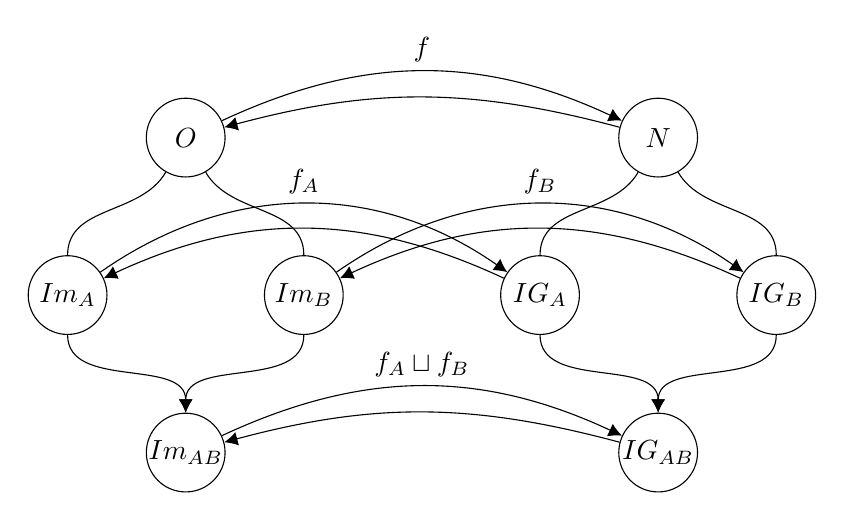
\begin{tikzpicture} 
    \path
    (-3,4) node[circle,draw,minimum size=10mm,inner sep=0pt](ME) {$O$}
    (-4.5,2) node[circle,draw,minimum size=10mm,inner sep=0pt](MA) {$Im_A$}
    (-1.5,2) node[circle,draw,minimum size=10mm,inner sep=0pt](MB) {$Im_B$}
    (-3,0) node[circle,draw,minimum size=10mm,inner sep=0pt](MAB) {$Im_{AB}$}
    
    (3,4) node[circle,draw,minimum size=10mm,inner sep=0pt](GN) {$N$}
    (1.5,2) node[circle,draw,minimum size=10mm,inner sep=0pt](GA) {$IG_A$}
    (4.5,2) node[circle,draw,minimum size=10mm,inner sep=0pt](GB) {$IG_B$}
    (3,0) node[circle,draw,minimum size=10mm,inner sep=0pt](GAB) {$IG_{AB}$};
    
    \path[]		
    (ME) [-, black, out=240, in=90] edge node[above] {} (MA)
    (ME) [-, black, out=300, in=90] edge node[above] {} (MB)
    
    (MA) [-{Latex[width=5]}, black, out=270, in=90] edge node[above] {} (MAB)
    (MB) [-{Latex[width=5]}, black, out=270, in=90] edge node[above] {} (MAB)
    
    (GN) [-, black, out=240, in=90] edge node[above] {} (GA)
    (GN) [-, black, out=300, in=90] edge node[above] {} (GB)
    
    (GA) [-{Latex[width=5]}, black, out=270, in=90] edge node[above] {} (GAB)
    (GB) [-{Latex[width=5]}, black, out=270, in=90] edge node[above] {} (GAB)
    
    (ME) [-{Latex[width=5]}, black, out=25, in=155] edge node[above] {$f$} (GN)
    (GN) [-{Latex[width=5]}, black, out=165, in=15] edge node[above] {} (ME)
    
    (MA) [-{Latex[width=5]}, black, out=35, in=145] edge node[above] {$f_A$} (GA)
    (GA) [-{Latex[width=5]}, black, out=155, in=25] edge node[above] {} (MA)
    
    (MB) [-{Latex[width=5]}, black, out=35, in=145] edge node[above] {$f_B$} (GB)
    (GB) [-{Latex[width=5]}, black, out=155, in=25] edge node[above] {} (MB)
    
    (MAB) [-{Latex[width=5]}, black, out=25, in=155] edge node[above] {$f_{A} \sqcup f_{B}$} (GAB)
    (GAB) [-{Latex[width=5]}, black, out=165, in=15] edge node[above] {} (MAB)
    ;
    \end{tikzpicture}
    \caption{Structure for transforming between instance models and instance graphs}
    \label{fig:transformation_framework:instance_models_and_instance_graphs:structure_instance_models_graphs}
\end{figure}

\cref{fig:transformation_framework:instance_models_and_instance_graphs:structure_instance_models_graphs} shows one more alternation of the structure proposed in \cref{sec:transformation_framework:structure}. This version of the structure is applied to instance models and instance graphs. As before, instance model $Im_A$ represents the partially build model which corresponds to instance graph $IG_A$ under the transformation function $f_A$. Instance model $Im_B$ represents the next building block to add to this model. It corresponds to instance graph $IG_B$ under the bijective transformation function $f_B$.

Instance models $Im_A$ and $Im_B$ are entirely distinct except for a set objects $O$, which means $O \subseteq Object_{Im_A} \land O \subseteq Object_{Im_B}$. In a similar way, instance graphs $IG_A$ and $IG_B$ are entirely distinct except for a set of nodes $N$, so $N \subseteq N_{IG_A} \land N \subseteq N_{IG_B}$.

Instance models $Im_A$ and $Im_B$ are combined into instance model $Im_{AB}$ using \cref{defin:transformation_framework:instance_models_and_instance_graphs:combining_instance_models:combine}. In a similar way instance graphs $IG_A$ and $IG_B$ are combined into instance graph $IG_{AB}$ using \cref{defin:transformation_framework:instance_models_and_instance_graphs:combining_instance_graphs:combine}. \cref{defin:transformation_framework:instance_models_and_instance_graphs:combining_instance_models:imod_combine_merge_correct} and \cref{defin:transformation_framework:instance_models_and_instance_graphs:combining_instance_graphs:ig_combine_merge_correct} respectively show that $Im_{AB}$ and $IG_{AB}$ are valid. Then \cref{defin:transformation_framework:instance_models_and_instance_graphs:combining_transformation_functions:combination_transformation_function_instance_model_instance_graph} and \cref{defin:transformation_framework:instance_models_and_instance_graphs:combining_transformation_functions:combination_transformation_function_instance_graph_instance_model} can be used to merge the transformation functions $f_A$ and $f_B$ into $f_{A} \sqcup f_{B}$, where \cref{defin:transformation_framework:instance_models_and_instance_graphs:combining_transformation_functions:ig_combine_mapping_correct} and \cref{defin:transformation_framework:instance_models_and_instance_graphs:combining_transformation_functions:ig_combine_mapping_function_correct} show that $f_{A} \sqcup f_{B}$ is again a valid transformation function transforming $Im_{AB}$ to $IG_{AB}$. Similarly, \cref{defin:transformation_framework:instance_models_and_instance_graphs:combining_transformation_functions:imod_combine_mapping_correct} and \cref{defin:transformation_framework:instance_models_and_instance_graphs:combining_transformation_functions:imod_combine_mapping_function_correct} show that the inverse function of $f_{A} \sqcup f_{B}$ is again a valid transformation function transforming $IG_{AB}$ to $Im_{AB}$.

\subsection{Combining instance models}
\label{subsec:transformation_framework:instance_models_and_instance_graphs:combining_instance_models}

The structure of \cref{fig:transformation_framework:instance_models_and_instance_graphs:structure_instance_models_graphs} shows that the instance models $Im_A$ and $Im_B$ are combined into one instance model $Im_{AB}$. This section provides the definition of this combination and its corresponding theorems. Please note that the definitions presented here are as generic as possible, and do not actively take into account that $Im_{A}$ and $Im_{B}$ are mostly distinct. This bit of information is added later as part of a theorem and proof.

\begin{defin}[Combination function on type models]
\label{defin:transformation_framework:instance_models_and_instance_graphs:combining_instance_models:combine}
$\mathrm{combine}$ is a binary function on two instance models which combines two instance models into one instance model. Assume $Im_A$ is an instance model typed by type model $Tm_A$ and $Im_B$ is an instance model typed by type model $Tm_B$, then $\mathrm{combine}(Im_A, Im_B)$ is typed by $\mathrm{combine}(Tm_A, Tm_B)$ and is defined as follows:
\begin{align*}
\mathrm{combine}(Im_A, Im_B) = \langle&
Object = Object_{Im_A} \cup Object_{Im_B} \\&
\mathrm{ObjectClass} = \mathrm{objectclass\_\!combine}(Im_A, Im_B) \\&
\mathrm{ObjectId} = \mathrm{objectid\_\!combine}(Im_A, Im_B) \\&
\mathrm{FieldValue} = \mathrm{fieldvalue\_\!combine}(Im_A, Im_B) \\&
\mathrm{DefaultValue} = \mathrm{defaultvalue\_\!combine}(Im_A, Im_B)\rangle
\end{align*}

In which $\mathrm{objectclass\_\!combine}$ is given as part of \cref{defin:transformation_framework:instance_models_and_instance_graphs:combining_instance_models:objectclass_combine}, $\mathrm{objectid\_\!combine}$ as part of \cref{defin:transformation_framework:instance_models_and_instance_graphs:combining_instance_models:objectid_combine}, $\mathrm{fieldvalue\_\!combine}$ as part of \cref{defin:transformation_framework:instance_models_and_instance_graphs:combining_instance_models:fieldvalue_combine} and $\mathrm{defaultvalue\_\!combine}$ as part of \cref{defin:transformation_framework:instance_models_and_instance_graphs:combining_instance_models:defaultvalue_combine}.
\isabellelref{imod_combine}{Ecore.Instance_Model_Combination}
\end{defin}

The combination of two instance models knows a surprisingly simple definition. This is mostly caused by the fact that an instance model only contains of a set of objects, which has some properties. The properties of each object are specified by the different functions, which will be introduced in the following definitions.

First, the function for the combination of object classes is discussed.

\begin{defin}[Combination function for object classes]
\label{defin:transformation_framework:instance_models_and_instance_graphs:combining_instance_models:objectclass_combine}
$\mathrm{objectclass\_\!combine}$ is a partial function on two instance models which returns a new function \\$Object_{Im_{AB}} \Rightarrow Class_{Tm_{AB}}$. It is defined as follows:
\begin{multline*}
    \mathrm{objectclass\_\!combine}(Im_{A}, Im_{B}, o) = \\
        \begin{cases}
        \mathrm{ObjectClass}_{Im_A}(o) & \mathrm{if }\ o \in Object_{Im_A} \cap Object_{Im_B} \land \mathrm{ObjectClass}_{Im_A}(o) = \mathrm{ObjectClass}_{Im_B}(o) \\
        \mathrm{ObjectClass}_{Im_A}(o) & \mathrm{if }\ o \in Object_{Im_A} \setminus Object_{Im_B} \\
        \mathrm{ObjectClass}_{Im_B}(o) & \mathrm{if }\ o \in Object_{Im_B} \setminus Object_{Im_A}
    \end{cases}
\end{multline*}
\isabellelref{imod_combine_object_class}{Ecore.Instance_Model_Combination}
\end{defin}

The combination of two instance models knows a surprisingly simple definition. Because an instance model is essentially a set of objects with properties, no complex definition is needed. The properties of each object are specified by the different functions, which will be introduced in the following definitions.

First, the function of the combination of object classes is discussed.

\begin{defin}[Combination function for object identifiers]
\label{defin:transformation_framework:instance_models_and_instance_graphs:combining_instance_models:objectid_combine}
$\mathrm{objectid\_\!combine}$ is a partial function on two instance models which returns a new function \\$Object_{Im_{AB}} \Rightarrow Name$. It is defined as follows:
\begin{multline*}
    \mathrm{objectid\_\!combine}(Im_{A}, Im_{B}, o) = \\
        \begin{cases}
        \mathrm{ObjectId}_{Im_A}(o) & \mathrm{if }\ o \in Object_{Im_A} \cap Object_{Im_B} \land \mathrm{ObjectId}_{Im_A}(o) = \mathrm{ObjectId}_{Im_B}(o) \\
        \mathrm{ObjectId}_{Im_A}(o) & \mathrm{if }\ o \in Object_{Im_A} \setminus Object_{Im_B} \\
        \mathrm{ObjectId}_{Im_B}(o) & \mathrm{if }\ o \in Object_{Im_B} \setminus Object_{Im_A}
    \end{cases}
\end{multline*}
\isabellelref{imod_combine_object_id}{Ecore.Instance_Model_Combination}
\end{defin}

As mentioned before, the definition of the combination function of object identifiers is very similar to the definition of the combination function of object classes. If an object only occurs in one of the instance models, its identifier is copied over. If an object appears in both instance models, they must have the same identifier already in order to have an identifier in the final model.

A careful reader might notice that the behaviour of the function is strange. Theoretically, it might give rise to double identities, which is undesired. As will be shown later, the combination function and theorems assume that the identities of the models are already distinct. This assumption is fair, as it is possible to redefine two instance models to have distinct identities, without loss of significance.

The following definition describes the combination of field values.

\begin{defin}[Combination function for field values]
\label{defin:transformation_framework:instance_models_and_instance_graphs:combining_instance_models:fieldvalue_combine}
$\mathrm{fieldvalue\_\!combine}$ is a partial function on two instance models which returns a new function \\$(Object_{Im_{AB}} \times Field_{Tm_{AB}}) \Rightarrow Value_{Im_{AB}}$. It is defined as follows:
\begin{multline*}
    \mathrm{fieldvalue\_\!combine}(Im_A, Im_B, ( o, f )) = \\
    \begin{cases}
        \mathrm{FieldValue}_{Im_A}(( o, f )) & \mathrm{if}\ o \in Object_{Im_A} \cap Object_{Im_B}\ \land\\&\quad f \in \mathrm{fields}_{Tm_A}(\mathrm{ObjectClass}_{Im_A}(o))\ \land\\&\quad f \in \mathrm{fields}_{Tm_B}(\mathrm{ObjectClass}_{Im_B}(o))\ \land\\&\quad \mathrm{FieldValue}_{Im_A}(( o, f )) = \mathrm{FieldValue}_{Im_B}(( o, f )) \\
        \mathrm{FieldValue}_{Im_A}(( o, f )) & \mathrm{if}\ o \in Object_{Im_A} \land f \in \mathrm{fields}_{Tm_A}(\mathrm{ObjectClass}_{Im_A}(o))\ \land\\&\quad (o \not\in Object_{Im_B} \lor f \not\in \mathrm{fields}_{Tm_B}(\mathrm{ObjectClass}_{Im_B}(o))) \\
        \mathrm{FieldValue}_{Im_B}(( o, f )) & \mathrm{if}\ o \in Object_{Im_B} \land f \in \mathrm{fields}_{Tm_B}(\mathrm{ObjectClass}_{Im_B}(o))\ \land\\&\quad (o \not\in Object_{Im_A} \lor f \not\in \mathrm{fields}_{Tm_A}(\mathrm{ObjectClass}_{Im_A}(o)))
    \end{cases}
\end{multline*}
\isabellelref{imod_combine_field_value}{Ecore.Instance_Model_Combination}
\end{defin}

The definition of the combination function of field values is a lot more complicated than the previous ones. The function domain causes this complexity. Not every combination of an object and a field has a value. An object only has values for those fields that are defined for its class or superclasses.

When a value is set on one of the instance models, but not the other, the value is copied. Furthermore, if a combination of object and field is set for both instance models and the value is the same, it is also copied. Please note that equality is used here, instead of equivalence. This property is to support some mathematical properties later on. Since the transformation framework will not allow for shared fields anyhow, this will not impose problems later.

The last function that needs to be defined is the combination function for default values. It is given in the following definition.

\begin{defin}[Combination function for default values]
\label{defin:transformation_framework:instance_models_and_instance_graphs:combining_instance_models:defaultvalue_combine}
$\mathrm{defaultvalue\_\!combine}$ is a partial function on two instance models which returns a new function \\$Constant_{Tm_{AB}} \Rightarrow Value_{Im_{AB}}$. It is defined as follows:
\begin{multline*}
    \mathrm{defaultvalue\_\!combine}(Im_{A}, Im_{B}, c) = \\
    \begin{cases}
        \mathrm{DefaultValue}_{Im_A}(c) & \mathrm{if }\ c \in Constant_{Tm_A} \cap Constant_{Tm_B}\ \land\\&\quad \mathrm{DefaultValue}_{Im_A}(c) = \mathrm{DefaultValue}_{Im_B}(c) \\
        \mathrm{DefaultValue}_{Im_A}(c) & \mathrm{if }\ c \in Constant_{Tm_A} \setminus Constant_{Tm_B} \\
        \mathrm{DefaultValue}_{Im_B}(c) & \mathrm{if }\ c \in Constant_{Tm_B} \setminus Constant_{Tm_A}
    \end{cases}
\end{multline*}
\isabellelref{imod_combine_default_value}{Ecore.Instance_Model_Combination}
\end{defin}

The definition of the combination function of default values is very similar to the combination function of constant types of type models (see \cref{defin:transformation_framework:type_models_and_type_graphs:combining_type_models:consttype_combine}). This function gives values to constants defined on the type model level. When a constant only appears in the type model of one of the instance models, the value can be copied from that instance model. This behaviour is logical since the other instance model cannot have a value set for that constant. If a constant is set for both of the corresponding type models, the value set on the instance models must be the same. If this is the case, the value can be copied over. This behaviour is desired, as the value for a constant should not change after the combination of two instance models.

Like the last definition, equality is used here to compare the values, instead of equivalence. Once more, this has been done to support some mathematical properties later on. Since the transformation framework will not allow for shared constants anyhow, this will not impose problems later.

With all definitions in place, it is possible to provide an example. Let us return to the multi-protocol chat application example introduced in \cref{fig:transformation_framework:type_models_and_type_graphs:combining_type_models:combine_example} of \cref{subsec:transformation_framework:type_models_and_type_graphs:combining_type_models}. An instance model for $Tm_{Chat}$ (\cref{fig:transformation_framework:type_models_and_type_graphs:combining_type_models:combine_example_tmod1}) could have an instance of a $\type{Thread}$ with some $\type{Message}$s. Formally, the instance model could look as follows:

\begin{align*}
Im_{Chat} =\ &\langle&
Object =\ &\{ 1, 2, 3 \} \\&&
\mathrm{ObjectClass} =\ &\{
( 1, \type{.Thread} ),
( 2, \type{.Message} ),
( 3, \type{.Message} )
\} \\&&
\mathrm{ObjectId} =\ &\{
( 1, \text{Thread42} ),
( 2, \text{Message4084} ),
( 3, \text{Message4093} )
\} \\&&
\mathrm{FieldValue} =\ &\Big\{
\Big( \big( 1, ( \type{.Thread}, \type{id} ) \big), \big[ \type{string}, \text{``BLUB-E\_Thread\_01''} \big] \Big),\\&&&
\Big( \big( 1, ( \type{.Thread}, \type{proto} ) \big), \big[ \type{enum}, ( \type{.Protocol}, \type{BLUB\!-\!E} ) \big] \Big),\\&&&
\Big( \big( 1, ( \type{.Thread}, \type{messages} ) \big), \big[ \type{seqof}, \big\langle [ \type{obj}, 2 ], [ \type{obj}, 3 ] \big\rangle \big] \Big),\\&&&
\Big( \big( 2, ( \type{.Message}, \type{text} ) \big), \big[ \type{string}, \text{``This is a test''} \big] \Big),\\&&&
\Big( \big( 3, ( \type{.Message}, \type{text} ) \big), \big[ \type{string}, \text{``Did you receive it?''} \big] \Big)
\Big\} \\&&
\mathrm{DefaultValue} =\ &\{\}
\\&\rangle
\end{align*}

A visual representation of this instance model is included in \cref{fig:transformation_framework:instance_models_and_instance_graphs:combining_instance_models:combine_example_imod1}. Now, assume that there also exists some instance model that is typed by the extension represented by $Tm_{Extension}$. This instance model introduces a $\type{Contact}$ instance for the $\type{Thread}$ instance in $Im_{Chat}$. Formally, this instance model could be defined as follows:

\begin{align*}
Im_{Extension} =\ &\langle&
Object =\ &\{ 1, 4 \} \\&&
\mathrm{ObjectClass} =\ &\{
( 1, \type{.Thread} ),
( 4, \type{.Contact} )
\} \\&&
\mathrm{ObjectId} =\ &\{
( 1, \text{Thread42} ),
( 4, \text{Broodkast} )
\} \\&&
\mathrm{FieldValue} =\ &\Big\{
\Big( \big( 1, ( \type{.Thread}, \type{contact} ) \big), \big[ \type{obj}, 4 \big] \Big),\\&&&
\Big( \big( 4, ( \type{.Contact}, \type{id} ) \big), \big[ \type{data}, \text{``BLUB-E\_PubKey\_a8138''} \big] \Big),\\&&&
\Big( \big( 4, ( \type{.Contact}, \type{name} ) \big), \big[ \type{string}, \text{``Lukas''} \big] \Big)
\Big\} \\&&
\mathrm{DefaultValue} =\ &\{\}
\\&\rangle
\end{align*}

The visual representation of $Im_{Extension}$ is included in \cref{fig:transformation_framework:instance_models_and_instance_graphs:combining_instance_models:combine_example_imod2}. With these instance models formally defined, it is possible to combine them using \cref{defin:transformation_framework:instance_models_and_instance_graphs:combining_instance_models:combine}. This will yield the following model:

\begin{align*}
Im_{ChatExt} =\ &\langle&
Object =\ &\{ 1, 2, 3, 4 \} \\&&
\mathrm{ObjectClass} =\ &\{
( 1, \type{.Thread} ),
( 2, \type{.Message} ),
( 3, \type{.Message} ),
( 4, \type{.Contact} )
\} \\&&
\mathrm{ObjectId} =\ &\{
( 1, \text{Thread42} ),
( 2, \text{Message4084} ),
( 3, \text{Message4093} ),
( 4, \text{Broodkast} )
\} \\&&
\mathrm{FieldValue} =\ &\Big\{
\Big( \big( 1, ( \type{.Thread}, \type{id} ) \big), \big[ \type{string}, \text{``BLUB-E\_Thread\_01''} \big] \Big),\\&&&
\Big( \big( 1, ( \type{.Thread}, \type{proto} ) \big), \big[ \type{enum}, ( \type{.Protocol}, \type{BLUB\!-\!E} ) \big] \Big),\\&&&
\Big( \big( 1, ( \type{.Thread}, \type{messages} ) \big), \big[ \type{seqof}, \big\langle [ \type{obj}, 2 ], [ \type{obj}, 3 ] \big\rangle \big] \Big),\\&&&
\Big( \big( 1, ( \type{.Thread}, \type{contact} ) \big), \big[ \type{obj}, 4 \big] \Big),\\&&&
\Big( \big( 2, ( \type{.Message}, \type{text} ) \big), \big[ \type{string}, \text{``This is a test''} \big] \Big),\\&&&
\Big( \big( 3, ( \type{.Message}, \type{text} ) \big), \big[ \type{string}, \text{``Did you receive it?''} \big] \Big),\\&&&
\Big( \big( 4, ( \type{.Contact}, \type{id} ) \big), \big[ \type{data}, \text{``BLUB-E\_PubKey\_a8138''} \big] \Big),\\&&&
\Big( \big( 4, ( \type{.Contact}, \type{name} ) \big), \big[ \type{string}, \text{``Lukas''} \big] \Big)
\Big\} \\&&
\mathrm{DefaultValue} =\ &\{\}
\\&\rangle
\end{align*}

A visual representation of this combined model is included as \cref{fig:transformation_framework:instance_models_and_instance_graphs:combining_instance_models:combine_example_imod12}. Like the example for the combination of type models, this example shows that the definition of the combination of instance models is useful. It allows to build larger models out of smaller building blocks. Furthermore, the example shows that the combination of the two instance models is typed by the combination of its corresponding type models.

\begin{figure}
    \centering
    \begin{subfigure}{\textwidth}
        \centering
        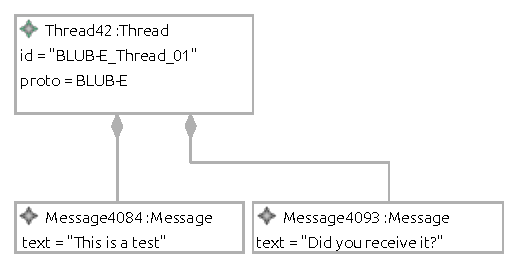
\includegraphics{images/04_transformation_framework/instance_models_combination/chat_instance_partial1.pdf}
        \caption{The chat application instance model $Im_{Chat}$}
        \label{fig:transformation_framework:instance_models_and_instance_graphs:combining_instance_models:combine_example_imod1}
    \end{subfigure}
    \par\medskip
    \begin{subfigure}{\textwidth}
        \centering
        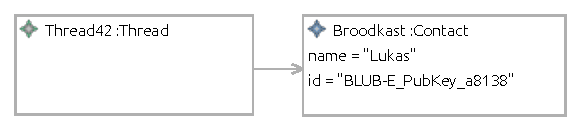
\includegraphics{images/04_transformation_framework/instance_models_combination/chat_instance_partial2.pdf}
        \caption{The contact extension instance model $Im_{Extension}$}
        \label{fig:transformation_framework:instance_models_and_instance_graphs:combining_instance_models:combine_example_imod2}
    \end{subfigure}
    \par\medskip
    \begin{subfigure}{\textwidth}
        \centering
        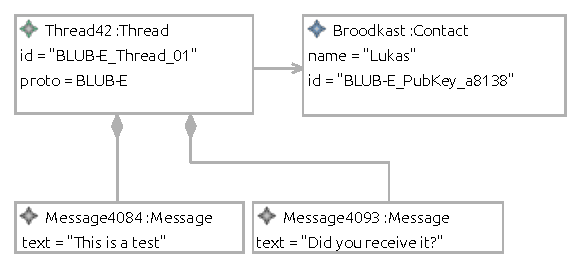
\includegraphics{images/04_transformation_framework/instance_models_combination/chat_instance_combined.pdf}
        \caption{The extended chat application instance model $Im_{ChatExt}$}
        \label{fig:transformation_framework:instance_models_and_instance_graphs:combining_instance_models:combine_example_imod12}
    \end{subfigure}
    \caption{Example of the combination of type models}
    \label{fig:transformation_framework:instance_models_and_instance_graphs:combining_instance_models:combine_example}
\end{figure}

Although the definitions of the combination of instance models are given, no mathematical properties or theorems are defined yet. Some mathematical properties hold for the combination of instance models, that will be presented in the following theorems.

\begin{thm}[Commutativity of the combination of instance models]
\label{defin:transformation_framework:instance_models_and_instance_graphs:combining_instance_models:imod_combine_commute}
Assume that $Im_A$ and $Im_B$ are instance models, then the $\mathrm{combine}$ function is commutative:
\begin{equation*}
    \mathrm{combine}(Im_A, Im_B) = \mathrm{combine}(Im_B, Im_A)
\end{equation*}
\isabellelref{imod_combine_commute}{Ecore.Instance_Model_Combination}
\end{thm}

\begin{thm}[Associativity of the combination of instance models]
\label{defin:transformation_framework:instance_models_and_instance_graphs:combining_instance_models:imod_combine_assoc}
Assume that $Im_A$, $Im_B$ and $Im_C$ are instance models, then the $\mathrm{combine}$ function is associative:
\begin{equation*}
    \mathrm{combine}(\mathrm{combine}(Im_A, Im_B), Im_C) = \mathrm{combine}(Im_A, \mathrm{combine}(Im_B, Im_C))
\end{equation*}
\isabellelref{imod_combine_assoc}{Ecore.Instance_Model_Combination}
\end{thm}

\begin{thm}[Idempotence of the combination of instance models]
\label{defin:transformation_framework:instance_models_and_instance_graphs:combining_instance_models:imod_combine_idemp}
Assume that $Im_A$ is an instance model and that it is valid in the sense of \cref{defin:formalisations:ecore_formalisation:instance_models:model_validity}. Then the following property holds:
\begin{equation*}
    \mathrm{combine}(Im_A, Im_A) = Im_A
\end{equation*}
\isabellelref{imod_combine_idemp_alt}{Ecore.Instance_Model_Combination}
\end{thm}

These properties follow directly from \cref{defin:transformation_framework:instance_models_and_instance_graphs:combining_instance_models:combine}, but the corresponding proofs will not be included here. It should be noted that these properties are indeed proven correct as part of this thesis, and the corresponding proofs are validated within Isabelle.

Besides these properties, the combination of instance models also has an identity element. The empty instance model represents this identity element, but it needs to be defined first:

\begin{defin}[Empty instance model]
\label{defin:transformation_framework:instance_models_and_instance_graphs:combining_instance_models:empty_instance_model}
Let $Im_{\epsilon}$ be the empty instance model. It is typed by the empty type model $Tm_{\epsilon}$. $Im_{\epsilon}$ is defined as:
\begin{align*}
Im_{\epsilon} = \langle&
Object = \{\} \\&
\mathrm{ObjectClass} = undefined \\&
\mathrm{ObjectId} = undefined \\&
\mathrm{FieldValue} = undefined \\&
\mathrm{DefaultValue} = undefined\rangle
\end{align*}
\end{defin}

\begin{thm}[Correctness of the empty type model]
\label{defin:transformation_framework:instance_models_and_instance_graphs:combining_instance_models:imod_empty_correct}
The empty instance model, $Im_{\epsilon}$, is valid with respect to
\cref{defin:formalisations:ecore_formalisation:instance_models:model_validity}.
\isabellelref{imod_empty_correct}{Ecore.Instance_Model}
\end{thm}

The proof for the correctness of the empty instance model is trivial. Still, a validated version of this proof can be found within the Isabelle theories of this thesis.

As mentioned earlier, the empty instance model acts as an identity element when combining two instance models. The following theorem specifies this behaviour.

\begin{thm}[Identity of the combination of instance models]
\label{defin:transformation_framework:instance_models_and_instance_graphs:combining_instance_models:imod_combine_identity}
Assume that $Im_A$ is an instance model and that it is valid in the sense of \cref{defin:formalisations:ecore_formalisation:instance_models:model_validity}. Then $Im_{\epsilon}$ acts as an identity element in the combination function:
\begin{equation*}
    \mathrm{combine}(Im_{\epsilon}, Im_A) = Im_A
\end{equation*}
\isabellelref{imod_combine_identity_alt}{Ecore.Instance_Model_Combination}
\end{thm}

Once more, the proof of this theorem follows directly from the definition. Therefore, the corresponding proof will not be included here, but a validated version can be found within the Isabelle theories of this thesis.

A final desired property for the combination of instance models is a correctness property. \cref{defin:transformation_framework:instance_models_and_instance_graphs:combining_instance_models:imod_combine_correct} defines the theorem under which the combination of instance models is a valid instance model. Please note that this theorem is a generic theorem, which does not take into account that the instance models are mostly distinct.

\begin{thm}[Validity of the combination of instance models]
\label{defin:transformation_framework:instance_models_and_instance_graphs:combining_instance_models:imod_combine_correct}
Assume that $Im_A$ and $Im_B$ are valid instance models in the sense of \cref{defin:formalisations:ecore_formalisation:instance_models:model_validity}. Assume that $Im_A$ is typed by type model $Tm_A$. Furthermore, assume that $Im_B$ is typed by type model $Tm_B$. $Tm_A$ and $Tm_B$ are consistent by definition. Also assume that $Tm_{AB} = \mathrm{combine}(Tm_A, Tm_B)$ is consistent in the sense of \cref{defin:formalisations:ecore_formalisation:type_models:type_model_consistency}. Finally, assume the following properties:
\begin{itemize}
    \item For all shared objects, the object class must be the same in both instance models: $\forall o \in Object_{Im_A} \cap Object_{Im_B}\!: \mathrm{ObjectClass}_{Im_A}(o) = \mathrm{ObjectClass}_{Im_B}(o)$.
    \item For all shared objects, the object id must be the same in both instance models: $\forall o \in Object_{Im_A} \cap Object_{Im_B}\!: \mathrm{ObjectId}_{Im_A}(o) = \mathrm{ObjectId}_{Im_B}(o)$.
    \item For all shared constants within the corresponding type graphs, the default value must be the same in both instance models: $\forall c \in Constant_{Tm_A} \cap Constant_{Tm_B}\!:$\\$\mathrm{DefaultValue}_{Im_A}(c) = \mathrm{DefaultValue}_{Im_B}(c)$.
    \item The identifiers must be unique across both instance models: $\forall o_1 \in Object_{Im_A} \setminus Object_{Im_B} \land o_2 \in Object_{Im_B} \setminus Object_{Im_A}\!: \mathrm{ObjectId}_{Im_A}(o_1) = \mathrm{ObjectId}_{Im_B}(o_2) \implies o_1 = o_2$.
    \item If a field value is set for a combination of an object and field in both instance models, that field value must be the same in both instance models: $\forall o \in Object_{Im_A} \cap Object_{Im_B}\ \land$\\$f \in \mathrm{fields}_{Tm_A}(\mathrm{ObjectClass}_{Im_A}(o)) \cap \mathrm{fields}_{Tm_B}(\mathrm{ObjectClass}_{Im_B}(o))\!:$\\$\mathrm{FieldValue}_{Im_A}(( o, f )) = \mathrm{FieldValue}_{Im_B}(( o, f ))$.
    \item If an object needs a field value in the combination of $Im_A$ and $Im_B$, but this field value is not set in $Im_A$, then it must be set in $Im_B$:
    $\forall o \in Object_{Im_A} \land f \not\in \mathrm{fields}_{Tm_A}(\mathrm{ObjectClass}_{Im_A}(o))\!:
    f \in \mathrm{fields}_{Tm_{AB}}(\mathrm{ObjectClass}_{\mathrm{combine}(Im_A, Im_B)}(o)) \implies$\\$
    o \in Object_{Im_B} \land f \in \mathrm{fields}_{Tm_B}(\mathrm{ObjectClass}_{Im_B}(o))$.
    \item If an object needs a field value in the combination of $Im_A$ and $Im_B$, but this field value is not set in $Im_B$, then it must be set in $Im_A$:
    $\forall o \in Object_{Im_B} \land f \not\in \mathrm{fields}_{Tm_B}(\mathrm{ObjectClass}_{Im_B}(o))\!:
    f \in \mathrm{fields}_{Tm_{AB}}(\mathrm{ObjectClass}_{\mathrm{combine}(Im_A, Im_B)}(o)) \implies$\\$
    o \in Object_{Im_A} \land f \in \mathrm{fields}_{Tm_A}(\mathrm{ObjectClass}_{Im_A}(o))$.
    \item For field values copied from $Im_A$ that are in $ContainerValue_{Im_A}$, the combined multiplicity must be correct: $\forall o \in Object_{Im_A}\ \land f \in \mathrm{fields}_{Tm_A}(\mathrm{ObjectClass}_{Im_A}(o))\ \land$\\$f \in Field_{Tm_B}\!: \mathrm{FieldValue}_{Im_A}(( o, f )) \in ContainerValue_{Im_A} \implies$\\$\mathrm{lower}_{Tm_{AB}}(\mathrm{FieldSig}_{Tm_{AB}}(f)) \leq |\mathrm{FieldValue}_{Im_A}(( o, f ))|\ \land$\\$|\mathrm{FieldValue}_{Im_A}(( o, f ))| \leq \mathrm{upper}_{Tm_{AB}}(\mathrm{FieldSig}_{Tm_{AB}}(f))$.
    \item For field values copied from $Im_B$ that are in $ContainerValue_{Im_B}$, the combined multiplicity must be correct: $\forall o \in Object_{Im_B}\ \land f \in \mathrm{fields}_{Tm_B}(\mathrm{ObjectClass}_{Im_B}(o))\ \land$\\$f \in Field_{Tm_A}\!: \mathrm{FieldValue}_{Im_B}(( o, f )) \in ContainerValue_{Im_B} \implies$\\$\mathrm{lower}_{Tm_{AB}}(\mathrm{FieldSig}_{Tm_{AB}}(f)) \leq |\mathrm{FieldValue}_{Im_B}(( o, f ))|\ \land$\\$|\mathrm{FieldValue}_{Im_B}(( o, f ))| \leq \mathrm{upper}_{Tm_{AB}}(\mathrm{FieldSig}_{Tm_{AB}}(f))$.
    \item If there exists a containment property in $Tm_{AB}$, the satisfaction formula for containment properties must be satisfied: $\forall o \in Object_{Im_A} \cup Object_{Im_B}\!:$\\$\big|\big\{ \big( ( f\!o, f\!\!f ), f\!v \big) \mid \big( ( f\!o, f\!\!f ), fv \big) \in \mathrm{FieldValue}_{\mathrm{combine}(Im_A, Im_B)} \land [ \type{obj}, o ] = f\!v \land f\!\!f \in CR_{Tm_{AB}} \big\}\big| \leq 1$
    \item There may be no cycles in the containment edges of the combined instance model: $\big\{ (f\!o, f\!v) \mid \big( ( f\!o, f\!\!f ), f\!v \big) \in \mathrm{FieldValue}_{\mathrm{combine}(Im_A, Im_B)} \land f\!\!f \in CR_{Tm_{AB}} \big\}$ is acyclic.
    \item The identity properties must remain satisfied when combining objects from different instance models: $\forall [ \type{identity}, c, A ] \in Prop_{Tm_{A}} \land [ \type{identity}, c, A ] \in Prop_{Tm_{B}} \land o_1 \in Object_{Im_A} \setminus Object_{Im_B} \land o_2 \in Object_{Im_B} \setminus Object_{Im_A} \land \mathrm{ObjectClass}_{Im_A}(o_1) = c \land \mathrm{ObjectClass}_{Im_B}(o_2) = c \land a \in A\!: \mathrm{FieldValue}_{Im_A}(( o_1, a )) \equiv_{\mathrm{combine}(Im_A, Im_B)} \mathrm{FieldValue}_{Im_B}(( o_2, a )) \implies o_1 = o_2$.
    \item The opposite properties must remain satisfied when combining objects from different instance models: $\forall [ \type{opposite}, r_1, r_2 ] \in Prop_{Tm_{A}} \land [ \type{opposite}, r_1, r_2 ] \in Prop_{Tm_{B}}\ \land$\\$o_1 \in Object_{Im_A} \land (o_1 \not\in Object_{Im_B} \lor r_1 \not\in \mathrm{fields}_{Tm_B}(\mathrm{ObjectClass}_{Im_B}(o_1)))\ \land$\\$o_2 \in Object_{Im_B} \land (o_2 \not\in Object_{Im_A} \lor r_2 \not\in \mathrm{fields}_{Tm_A}(\mathrm{ObjectClass}_{Im_A}(o_2))) \implies$\\$ \mathrm{edgeCount}_{Im_A}(o_1, r_1, o_2) = \mathrm{edgeCount}_{Im_B}(o_2, r_2, o_1)$.
\end{itemize}

Then $\mathrm{combine}(Im_A, Im_B)$ is a valid instance model in the sense of \cref{defin:formalisations:ecore_formalisation:instance_models:model_validity}
\isabellelref{imod_combine_correct}{Ecore.Instance_Model_Combination}
\end{thm}

\begin{proof}
To proof that $\mathrm{combine}(Im_A, Im_B)$ is a valid instance model, it needs to be shown that\\ $\mathrm{combine}(Im_A, Im_B)$ gives rise to a valid structure for an instance model and that \cref{defin:formalisations:ecore_formalisation:instance_models:model_validity} holds. For readability, define $Im_{AB}$ to be $\mathrm{combine}(Im_A, Im_B)$.

\emph{Structural properties}
\begin{itemize}
    \item For each object $o$, $\mathrm{ObjectClass}_{Im_{AB}}(o)$ must be an element of $Class_{Tm_{AB}}$.

    If $o \in Object_{Im_A} \setminus Object_{Im_B}$, then $\mathrm{ObjectClass}_{Im_{AB}}(o) \in Class_{Tm_{AB}}$.
    
    Similarly, if $o \in Object_{Im_B} \setminus Object_{Im_A}$, then $\mathrm{ObjectClass}_{Im_{AB}}(o) \in Class_{Tm_{AB}}$.
    
    If $o \in Object_{Im_A} \cap Object_{Im_B}$, then $\mathrm{ObjectClass}_{Im_{A}}(o) = \mathrm{ObjectClass}_{Im_{B}}(o)$ by assumption. Therefore $\mathrm{ObjectClass}_{Im_{AB}}(o) \in Class_{Tm_{AB}}$.


    \item For each object $o$, $\mathrm{ObjectId}_{Im_{AB}}(o)$ must be an element of $Name$.
    
    If $o \in Object_{Im_A} \setminus Object_{Im_B}$, then $\mathrm{ObjectId}_{Im_{AB}}(o) \in Name$.
    
    Similarly, if $o \in Object_{Im_B} \setminus Object_{Im_A}$, then $\mathrm{ObjectId}_{Im_{AB}}(o) \in Name$.
    
    If $o \in Object_{Im_A} \cap Object_{Im_B}$, then $\mathrm{ObjectId}_{Im_{A}}(o) = \mathrm{ObjectId}_{Im_{B}}(o)$ by assumption. Therefore $\mathrm{ObjectId}_{Im_{AB}}(o) \in Name$.
    
    
    \item For each object $o$, and $f \in \mathrm{fields}_{Tm_{AB}}(\mathrm{ObjectClass}_{Im_{AB}}(o))$, $\mathrm{FieldValue}_{Im_{AB}}(( o, f ))$ must be an element of $Value_{Im_{AB}}$.
    
    First, note that $Value_{Im_A} \cup Value_{Im_B} \subseteq Value_{Im_{AB}}$\\(see \isabelleref{imod_combine_value}{Ecore.Instance_Model_Combination}).
    
    If $o \in Object_{Im_A} \setminus Object_{Im_B}$, then $f \in \mathrm{fields}_{Tm_{A}}(\mathrm{ObjectClass}_{Im_{A}}(o))$ or \\$f \not\in \mathrm{fields}_{Tm_{A}}(\mathrm{ObjectClass}_{Im_{A}}(o))$.
    
    \begin{itemize}
        \item If $f \in \mathrm{fields}_{Tm_{A}}(\mathrm{ObjectClass}_{Im_{A}}(o))$, then $\mathrm{FieldValue}_{Im_{AB}}(( o, f )) = \mathrm{FieldValue}_{Im_{A}}(( o, f ))$ and, therefore, $\mathrm{FieldValue}_{Im_{AB}}(( o, f )) \in Value_{Im_{AB}}$.
        
        \item If $f \not\in \mathrm{fields}_{Tm_{A}}(\mathrm{ObjectClass}_{Im_{A}}(o))$, then by assumption, $f \in Object_{Im_B}$. However, $f \not\in Object_{Im_B}$, so this case is invalid.
    \end{itemize}
    
    If $o \in Object_{Im_B} \setminus Object_{Im_A}$, then $f \in \mathrm{fields}_{Tm_{B}}(\mathrm{ObjectClass}_{Im_{B}}(o))$ or \\$f \not\in \mathrm{fields}_{Tm_{B}}(\mathrm{ObjectClass}_{Im_{B}}(o))$.
    
    \begin{itemize}
        \item If $f \in \mathrm{fields}_{Tm_{B}}(\mathrm{ObjectClass}_{Im_{B}}(o))$, then $\mathrm{FieldValue}_{Im_{AB}}(( o, f )) = \mathrm{FieldValue}_{Im_{B}}(( o, f ))$ and, therefore, $\mathrm{FieldValue}_{Im_{AB}}(( o, f )) \in Value_{Im_{AB}}$.
        
        \item If $f \not\in \mathrm{fields}_{Tm_{B}}(\mathrm{ObjectClass}_{Im_{B}}(o))$, then by assumption, $f \in Object_{Im_A}$. However, $f \not\in Object_{Im_A}$, so this case is invalid.
    \end{itemize}
    
    If $o \in Object_{Im_A} \cap Object_{Im_B}$, then \\$f \in \mathrm{fields}_{Tm_{A}}(\mathrm{ObjectClass}_{Im_{A}}(o)) \cap \mathrm{fields}_{Tm_{B}}(\mathrm{ObjectClass}_{Im_{B}}(o))$ or \\$f \not\in \mathrm{fields}_{Tm_{A}}(\mathrm{ObjectClass}_{Im_{A}}(o))$ or $f \not\in \mathrm{fields}_{Tm_{B}}(\mathrm{ObjectClass}_{Im_{B}}(o))$.
    
    \begin{itemize}
        \item If $f \in \mathrm{fields}_{Tm_{A}}(\mathrm{ObjectClass}_{Im_{A}}(o)) \cap \mathrm{fields}_{Tm_{B}}(\mathrm{ObjectClass}_{Im_{B}}(o))$, then \\$\mathrm{FieldValue}_{Im_{AB}}(( o, f )) = \mathrm{FieldValue}_{Im_{A}}(( o, f ))$ and, therefore, \\$\mathrm{FieldValue}_{Im_{AB}}(( o, f )) \in Value_{Im_{AB}}$.
        
        \item If $f \not\in \mathrm{fields}_{Tm_{A}}(\mathrm{ObjectClass}_{Im_{A}}(o))$, then by assumption, $f \in \mathrm{fields}_{Tm_{B}}(\mathrm{ObjectClass}_{Im_{B}}(o))$. Therefore, $\mathrm{FieldValue}_{Im_{AB}}(( o, f )) = \mathrm{FieldValue}_{Im_{B}}(( o, f ))$ which means that \\$\mathrm{FieldValue}_{Im_{AB}}(( o, f )) \in Value_{Im_{AB}}$.
        
        \item If $f \not\in \mathrm{fields}_{Tm_{B}}(\mathrm{ObjectClass}_{Im_{B}}(o))$, then by assumption, $f \in \mathrm{fields}_{Tm_{A}}(\mathrm{ObjectClass}_{Im_{A}}(o))$. Therefore, $\mathrm{FieldValue}_{Im_{AB}}(( o, f )) = \mathrm{FieldValue}_{Im_{A}}(( o, f ))$ which means that \\$\mathrm{FieldValue}_{Im_{AB}}(( o, f )) \in Value_{Im_{AB}}$.
    \end{itemize}
    
    
    \item For each constant $c$ in $Constant_{Tm_{AB}}$, $\mathrm{DefaultValue}_{Im_{AB}}(c)$ must be an element of $Value_{Im_{AB}}$.
    
    First, note that $Value_{Im_A} \cup Value_{Im_B} \subseteq Value_{Im_{AB}}$\\(see \isabelleref{imod_combine_value}{Ecore.Instance_Model_Combination}).
    
    If $c \in Constant_{Tm_A} \setminus Constant_{Tm_B}$, then $\mathrm{DefaultValue}_{Im_{AB}}(c) \in Value_{Im_{AB}}$.
    
    Similarly, if $c \in Constant_{Tm_B} \setminus Constant_{Tm_A}$, then $\mathrm{DefaultValue}_{Im_{AB}}(c) \in Value_{Im_{AB}}$.
    
    If $c \in Constant_{Tm_A} \cap Constant_{Tm_B}$, then $\mathrm{DefaultValue}_{Im_{A}}(c) = \mathrm{DefaultValue}_{Im_{B}}(c)$ by assumption. Therefore $\mathrm{DefaultValue}_{Im_{AB}}(c) \in Value_{Im_{AB}}$.
\end{itemize}

\emph{Validity properties}
\begin{itemize}
    \item $\forall (( o, f ), v ) \in \mathrm{FieldValue}_{Im_{AB}}\!: v:_{Im} \mathrm{type}_{Tm_{AB}}(f)$
    
    If $o \in Object_{Im_A} \setminus Object_{Im_B}$, then $f \in \mathrm{fields}_{Tm_{A}}(\mathrm{ObjectClass}_{Im_{A}}(o))$ or \\$f \not\in \mathrm{fields}_{Tm_{A}}(\mathrm{ObjectClass}_{Im_{A}}(o))$.
    
    \begin{itemize}
        \item If $f \in \mathrm{fields}_{Tm_{A}}(\mathrm{ObjectClass}_{Im_{A}}(o))$, then $\mathrm{FieldValue}_{Im_{AB}}(( o, f )) = \mathrm{FieldValue}_{Im_{A}}(( o, f ))$. In this case $\mathrm{type}_{Tm_{AB}}(f) = \mathrm{type}_{Tm_{A}}(f)$ because types are preserved by $Tm_{AB}$. Therefore, $v:_{Im} \mathrm{type}_{Tm_{AB}}(f)$.
        
        \item If $f \not\in \mathrm{fields}_{Tm_{A}}(\mathrm{ObjectClass}_{Im_{A}}(o))$, then by assumption, $f \in Object_{Im_B}$. However, $f \not\in Object_{Im_B}$, so this case is invalid.
    \end{itemize}
    
    If $o \in Object_{Im_B} \setminus Object_{Im_A}$, then $f \in \mathrm{fields}_{Tm_{B}}(\mathrm{ObjectClass}_{Im_{B}}(o))$ or \\$f \not\in \mathrm{fields}_{Tm_{B}}(\mathrm{ObjectClass}_{Im_{B}}(o))$.
    
    \begin{itemize}
        \item If $f \in \mathrm{fields}_{Tm_{B}}(\mathrm{ObjectClass}_{Im_{B}}(o))$, then $\mathrm{FieldValue}_{Im_{AB}}(( o, f )) = \mathrm{FieldValue}_{Im_{B}}(( o, f ))$. In this case $\mathrm{type}_{Tm_{AB}}(f) = \mathrm{type}_{Tm_{B}}(f)$ because types are preserved by $Tm_{AB}$. Therefore, $v:_{Im} \mathrm{type}_{Tm_{AB}}(f)$.
        
        \item If $f \not\in \mathrm{fields}_{Tm_{B}}(\mathrm{ObjectClass}_{Im_{B}}(o))$, then by assumption, $f \in Object_{Im_A}$. However, $f \not\in Object_{Im_A}$, so this case is invalid.
    \end{itemize}
    
    If $o \in Object_{Im_A} \cap Object_{Im_B}$, then \\$f \in \mathrm{fields}_{Tm_{A}}(\mathrm{ObjectClass}_{Im_{A}}(o)) \cap \mathrm{fields}_{Tm_{B}}(\mathrm{ObjectClass}_{Im_{B}}(o))$ or \\$f \not\in \mathrm{fields}_{Tm_{A}}(\mathrm{ObjectClass}_{Im_{A}}(o))$ or $f \not\in \mathrm{fields}_{Tm_{B}}(\mathrm{ObjectClass}_{Im_{B}}(o))$.
    
    \begin{itemize}
        \item If $f \in \mathrm{fields}_{Tm_{A}}(\mathrm{ObjectClass}_{Im_{A}}(o)) \cap \mathrm{fields}_{Tm_{B}}(\mathrm{ObjectClass}_{Im_{B}}(o))$, then \\$\mathrm{FieldValue}_{Im_{AB}}(( o, f )) = \mathrm{FieldValue}_{Im_{A}}(( o, f ))$. In this case $\mathrm{type}_{Tm_{AB}}(f) = \mathrm{type}_{Tm_{A}}(f)$ because types are preserved by $Tm_{AB}$. Therefore, $v:_{Im} \mathrm{type}_{Tm_{AB}}(f)$.
        
        \item If $f \not\in \mathrm{fields}_{Tm_{A}}(\mathrm{ObjectClass}_{Im_{A}}(o))$, then by assumption, $f \in \mathrm{fields}_{Tm_{B}}(\mathrm{ObjectClass}_{Im_{B}}(o))$. Therefore, $\mathrm{FieldValue}_{Im_{AB}}(( o, f )) = \mathrm{FieldValue}_{Im_{B}}(( o, f ))$. Furthermore, $\mathrm{type}_{Tm_{AB}}(f) = \mathrm{type}_{Tm_{A}}(f)$ because types are preserved by $Tm_{AB}$. Therefore, $v:_{Im} \mathrm{type}_{Tm_{AB}}(f)$.
        
        \item If $f \not\in \mathrm{fields}_{Tm_{B}}(\mathrm{ObjectClass}_{Im_{B}}(o))$, then by assumption, $f \in \mathrm{fields}_{Tm_{A}}(\mathrm{ObjectClass}_{Im_{A}}(o))$. Therefore, $\mathrm{FieldValue}_{Im_{AB}}(( o, f )) = \mathrm{FieldValue}_{Im_{A}}(( o, f ))$. Furthermore, $\mathrm{type}_{Tm_{AB}}(f) = \mathrm{type}_{Tm_{A}}(f)$ because types are preserved by $Tm_{AB}$. Therefore, $v:_{Im} \mathrm{type}_{Tm_{AB}}(f)$.
    \end{itemize}
    
    
    \item $\forall (( o, f ), v ) \in \mathrm{FieldValue}_{Im_{AB}}\!: \mathrm{validMul}_{Im_{AB}}(v)$.
    
    If $o \in Object_{Im_A} \setminus Object_{Im_B}$, then $f \in \mathrm{fields}_{Tm_{A}}(\mathrm{ObjectClass}_{Im_{A}}(o))$ or \\$f \not\in \mathrm{fields}_{Tm_{A}}(\mathrm{ObjectClass}_{Im_{A}}(o))$.
    
    \begin{itemize}
        \item If $f \in \mathrm{fields}_{Tm_{A}}(\mathrm{ObjectClass}_{Im_{A}}(o))$, then $\mathrm{FieldValue}_{Im_{AB}}(( o, f )) = \mathrm{FieldValue}_{Im_{A}}(( o, f ))$. Because $Im_{A}$ is valid, $\mathrm{validMul}_{Im_{A}}(v)$ holds. If the multiplicity is preserved because $f \not\in Field_{Tm_B}$, then $\mathrm{validMul}_{Im_{AB}}(v)$. If the multiplicity is changed because $f \in Field_{Tm_B}$, then $\mathrm{validMul}_{Im_{AB}}(v)$ is proven by assumption.
        
        \item If $f \not\in \mathrm{fields}_{Tm_{A}}(\mathrm{ObjectClass}_{Im_{A}}(o))$, then by assumption, $f \in Object_{Im_B}$. However, $f \not\in Object_{Im_B}$, so this case is invalid.
    \end{itemize}
    
    If $o \in Object_{Im_B} \setminus Object_{Im_A}$, then $f \in \mathrm{fields}_{Tm_{B}}(\mathrm{ObjectClass}_{Im_{B}}(o))$ or \\$f \not\in \mathrm{fields}_{Tm_{B}}(\mathrm{ObjectClass}_{Im_{B}}(o))$.
    
    \begin{itemize}
        \item If $f \in \mathrm{fields}_{Tm_{B}}(\mathrm{ObjectClass}_{Im_{B}}(o))$, then $\mathrm{FieldValue}_{Im_{AB}}(( o, f )) = \mathrm{FieldValue}_{Im_{B}}(( o, f ))$. Because $Im_{B}$ is valid, $\mathrm{validMul}_{Im_{B}}(v)$ holds. If the multiplicity is preserved because $f \not\in Field_{Tm_A}$, then $\mathrm{validMul}_{Im_{AB}}(v)$. If the multiplicity is changed because $f \in Field_{Tm_A}$, then $\mathrm{validMul}_{Im_{AB}}(v)$ is proven by assumption.
        
        \item If $f \not\in \mathrm{fields}_{Tm_{B}}(\mathrm{ObjectClass}_{Im_{B}}(o))$, then by assumption, $f \in Object_{Im_A}$. However, $f \not\in Object_{Im_A}$, so this case is invalid.
    \end{itemize}
    
    If $o \in Object_{Im_A} \cap Object_{Im_B}$, then \\$f \in \mathrm{fields}_{Tm_{A}}(\mathrm{ObjectClass}_{Im_{A}}(o)) \cap \mathrm{fields}_{Tm_{B}}(\mathrm{ObjectClass}_{Im_{B}}(o))$ or \\$f \not\in \mathrm{fields}_{Tm_{A}}(\mathrm{ObjectClass}_{Im_{A}}(o))$ or $f \not\in \mathrm{fields}_{Tm_{B}}(\mathrm{ObjectClass}_{Im_{B}}(o))$.
    
    \begin{itemize}
        \item If $f \in \mathrm{fields}_{Tm_{A}}(\mathrm{ObjectClass}_{Im_{A}}(o)) \cap \mathrm{fields}_{Tm_{B}}(\mathrm{ObjectClass}_{Im_{B}}(o))$, then \\$\mathrm{FieldValue}_{Im_{AB}}(( o, f )) = \mathrm{FieldValue}_{Im_{A}}(( o, f ))$. In this case $\mathrm{validMul}_{Im_{AB}}(v)$ is proven by assumption since the multiplicity of $f$ has been combined into a new multiplicity.
        
        \item If $f \not\in \mathrm{fields}_{Tm_{A}}(\mathrm{ObjectClass}_{Im_{A}}(o))$, then by assumption, $f \in \mathrm{fields}_{Tm_{B}}(\mathrm{ObjectClass}_{Im_{B}}(o))$. Therefore, $\mathrm{FieldValue}_{Im_{AB}}(( o, f )) = \mathrm{FieldValue}_{Im_{B}}(( o, f ))$. Furthermore, because $Im_{B}$ is valid, $\mathrm{validMul}_{Im_{B}}(v)$ holds. If the multiplicity is preserved because $f \not\in Field_{Tm_A}$, then $\mathrm{validMul}_{Im_{AB}}(v)$. If the multiplicity is changed because $f \in Field_{Tm_A}$, then $\mathrm{validMul}_{Im_{AB}}(v)$ is proven by assumption.
        
        \item If $f \not\in \mathrm{fields}_{Tm_{B}}(\mathrm{ObjectClass}_{Im_{B}}(o))$, then by assumption, $f \in \mathrm{fields}_{Tm_{A}}(\mathrm{ObjectClass}_{Im_{A}}(o))$. Therefore, $\mathrm{FieldValue}_{Im_{AB}}(( o, f )) = \mathrm{FieldValue}_{Im_{A}}(( o, f ))$. Furthermore, because $Im_{A}$ is valid, $\mathrm{validMul}_{Im_{A}}(v)$ holds. If the multiplicity is preserved because $f \not\in Field_{Tm_B}$, then $\mathrm{validMul}_{Im_{AB}}(v)$. If the multiplicity is changed because $f \in Field_{Tm_B}$, then $\mathrm{validMul}_{Im_{AB}}(v)$ is proven by assumption.
    \end{itemize}
    
    
    \item $\forall p \in Prop_{Tm_{AB}}\!: Im \models p$
    
    Make a case distinction for the different possible properties.
    \begin{itemize}
        \item For $[ \type{abstract}, c ] \in Prop_{Tm_{AB}}$, use the fact that $Tm_{AB}$ is consistent to establish that abstract properties are only copied iff there are no instances of it in the combined instance graph (see \cref{defin:transformation_framework:type_models_and_type_graphs:combining_type_models:prop_combine} for details). Therefore, $Im \models [ \type{abstract}, c ]$.
        
        \item For $[ \type{containment}, r ] \in Prop_{Tm_{AB}}$, use the assumptions to prove that $Im \models [ \type{containment}, r ]$.
        
        \item For $[ \type{defaultValue}, f, v ] \in Prop_{Tm_{AB}}$, there is no specific satisfaction formula, therefore $Im \models [ \type{defaultValue}, f, v ]$.
        
        \item For $[ \type{identity}, c, A ] \in Prop_{Tm_{AB}}$, if the property was copied over from only one of the type models, then $Im \models [ \type{identity}, c, A ]$. This is the case because $c$ could not have been part of the other type model and therefore not occur in its instance models.
        
        If $[ \type{identity}, c, A ] \in Prop_{Tm_{AB}}$ was present in both type models, then the identity satisfaction formula will be correct for each pair of instances from $Im_{A}$ and each pair of instances from $Im_{B}$. To ensure that it is correct for mixed instance pairs, use the assumption specified. Then establish that $Im \models [ \type{identity}, c, A ]$.
        
        \item For $[ \type{keyset}, r, A ] \in Prop_{Tm_{AB}}$, it is clear that each value of $r$ in the combined instance graph is either the copied field value from $Im_{A}$ or the copied field value from $Im_{B}$. Since values are preserved, there can be no new objects added to an existing relation. Therefore, $Im \models [ \type{keyset}, r, A ]$.
        
        \item For $[ \type{opposite}, r, r' ] \in Prop_{Tm_{AB}}$, if the property was copied over from only one of the type models, then $Im \models [ \type{opposite}, r, r' ]$. This is the case because $r$ and $r'$ could not have been part of the other type model and therefore not occur in its instance models.
        
        If $[ \type{opposite}, r, r' ] \in Prop_{Tm_{AB}}$ was present in both type models, then the opposite satisfaction formula will be correct for each pair of instances from $Im_{A}$ and each pair of instances from $Im_{B}$. To ensure that it is correct for mixed instance pairs, use the assumption specified. Then establish that $Im \models [ \type{opposite}, r, r' ]$.
        
        \item For $[ \type{readonly}, f ] \in Prop_{Tm_{AB}}$, there is no specific satisfaction formula, therefore $Im \models [ \type{readonly}, f ]$.
    \end{itemize}
    
    
    \item $\forall c \in Constant_{Tm_{AB}}\!: \mathrm{DefaultValue}_{Im_{AB}}(c):_{Im_{AB}} \mathrm{ConstType}_{Tm_{AB}}(c)$.
    
    If $c \in Constant_{Tm_A} \setminus Constant_{Tm_B}$, then $\mathrm{DefaultValue}_{Im_{AB}}(c) = \mathrm{DefaultValue}_{Im_{A}}(c)$. Furthermore, $\mathrm{ConstType}_{Tm_{AB}}(c) = \mathrm{ConstType}_{Tm_{A}}(c)$. Therefore, \\$\mathrm{DefaultValue}_{Im_{AB}}(c):_{Im_{AB}} \mathrm{ConstType}_{Tm_{AB}}(c)$.
    
    Similarly, if $c \in Constant_{Tm_B} \setminus Constant_{Tm_A}$, then $\mathrm{DefaultValue}_{Im_{AB}}(c) = \mathrm{DefaultValue}_{Im_{B}}(c)$. Furthermore, $\mathrm{ConstType}_{Tm_{AB}}(c) = \mathrm{ConstType}_{Tm_{B}}(c)$. Therefore, \\$\mathrm{DefaultValue}_{Im_{AB}}(c):_{Im_{AB}} \mathrm{ConstType}_{Tm_{AB}}(c)$.
    
    If $c \in Constant_{Tm_A} \cap Constant_{Tm_B}$, then $\mathrm{DefaultValue}_{Im_{A}}(c) = \mathrm{DefaultValue}_{Im_{B}}(c)$ by assumption. Furthermore, $\mathrm{ConstType}_{Tm_{A}}(c) = \mathrm{ConstType}_{Tm_{B}}(c)$, since $Tm_{AB}$ is consistent. Therefore, $\mathrm{DefaultValue}_{Im_{AB}}(c):_{Im_{AB}} \mathrm{ConstType}_{Tm_{AB}}(c)$.
    
    
    \item $Tm_{AB}$ is consistent, as defined in \cref{defin:formalisations:ecore_formalisation:type_models:type_model_consistency}.
    
    This is specified to be true by assumption.
\end{itemize}

The proofs of all these individual properties complete the entire proof.
\end{proof}

As explained before, \cref{defin:transformation_framework:instance_models_and_instance_graphs:combining_instance_models:imod_combine_correct} does not take into account that the instance models are supposed to be distinct except for a set of objects. Furthermore, it does not take into account that the corresponding type models are supposed to be distinct except for a set of types. The following lemma is an alternation of the previous theorem, which takes these properties into account.

\begin{lem}[Consistency of the combination (mostly) distinct of instance models]
\label{defin:transformation_framework:instance_models_and_instance_graphs:combining_instance_models:imod_combine_merge_correct}
Assume that $Im_A$ and $Im_B$ are valid instance models in the sense of \cref{defin:formalisations:ecore_formalisation:instance_models:model_validity}. Assume that $Im_A$ is typed by type model $Tm_A$. Furthermore, assume that $Im_B$ is typed by type model $Tm_B$. $Tm_A$ and $Tm_B$ are consistent by definition. Also assume that $Tm_{AB} = \mathrm{combine}(Tm_A, Tm_B)$ is consistent in the sense of \cref{defin:formalisations:ecore_formalisation:type_models:type_model_consistency}. Moreover, assume that $Tm_{A}$ and $Tm_{B}$ are entirely distinct except for a set of types $T$. Also assume that $Im_{A}$ and $Im_{B}$ are entirely distinct except for a set of objects $O$. Finally, assume the following properties:
\begin{itemize}
    \item For all shared objects, the object class must be the same in both instance models: $\forall o \in Object_{Im_A} \cap Object_{Im_B}\!: \mathrm{ObjectClass}_{Im_A}(o) = \mathrm{ObjectClass}_{Im_B}(o)$.
    \item For all shared objects, the object id must be the same in both instance models: $\forall o \in Object_{Im_A} \cap Object_{Im_B}\!: \mathrm{ObjectId}_{Im_A}(o) = \mathrm{ObjectId}_{Im_B}(o)$.
    \item For all shared constants within the corresponding type graphs, the default value must be the same in both instance models: $\forall c \in Constant_{Tm_A} \cap Constant_{Tm_B}\!:$\\$\mathrm{DefaultValue}_{Im_A}(c) = \mathrm{DefaultValue}_{Im_B}(c)$.
    \item The identifiers must be unique across both instance models: $\forall o_1 \in Object_{Im_A} \setminus Object_{Im_B} \land o_2 \in Object_{Im_B} \setminus Object_{Im_A}\!: \mathrm{ObjectId}_{Im_A}(o_1) = \mathrm{ObjectId}_{Im_B}(o_2) \implies o_1 = o_2$.
    \item If an object needs a field value in the combination of $Im_A$ and $Im_B$, but this field value is not set in $Im_A$, then it must be set in $Im_B$:
    $\forall o \in Object_{Im_A} \land f \not\in \mathrm{fields}_{Tm_A}(\mathrm{ObjectClass}_{Im_A}(o))\!:
    f \in \mathrm{fields}_{Tm_{AB}}(\mathrm{ObjectClass}_{\mathrm{combine}(Im_A, Im_B)}(o)) \implies$\\$
    o \in Object_{Im_B} \land f \in \mathrm{fields}_{Tm_B}(\mathrm{ObjectClass}_{Im_B}(o))$.
    \item If an object needs a field value in the combination of $Im_A$ and $Im_B$, but this field value is not set in $Im_B$, then it must be set in $Im_A$:
    $\forall o \in Object_{Im_B} \land f \not\in \mathrm{fields}_{Tm_B}(\mathrm{ObjectClass}_{Im_B}(o))\!:
    f \in \mathrm{fields}_{Tm_{AB}}(\mathrm{ObjectClass}_{\mathrm{combine}(Im_A, Im_B)}(o)) \implies$\\$
    o \in Object_{Im_A} \land f \in \mathrm{fields}_{Tm_A}(\mathrm{ObjectClass}_{Im_A}(o))$.
    \item If there exists a containment property in $Tm_{AB}$, the satisfaction formula for containment properties must be satisfied: $\forall o \in Object_{Im_A} \cup Object_{Im_B}\!:$\\$\big|\big\{ \big( ( f\!o, f\!\!f ), f\!v \big) \mid \big( ( f\!o, f\!\!f ), fv \big) \in \mathrm{FieldValue}_{\mathrm{combine}(Im_A, Im_B)} \land [ \type{obj}, o ] = f\!v \land f\!\!f \in CR_{Tm_{AB}} \big\}\big| \leq 1$
    \item There may be no cycles in the containment edges of the combined instance model: $\big\{ (f\!o, f\!v) \mid \big( ( f\!o, f\!\!f ), f\!v \big) \in \mathrm{FieldValue}_{\mathrm{combine}(Im_A, Im_B)} \land f\!\!f \in CR_{Tm_{AB}} \big\}$ is acyclic.
\end{itemize}

Then $\mathrm{combine}(Im_A, Im_B)$ is a valid instance model in the sense of \cref{defin:formalisations:ecore_formalisation:instance_models:model_validity}.
\isabellelref{imod_combine_merge_correct}{Ecore.Instance_Model_Combination}
\end{lem}

\begin{proof}
Use \cref{defin:transformation_framework:instance_models_and_instance_graphs:combining_instance_models:imod_combine_correct} to show that $\mathrm{combine}(Im_A, Im_B)$ is a consistent type model. Use the assumptions given. Some assumptions of \cref{defin:transformation_framework:instance_models_and_instance_graphs:combining_instance_models:imod_combine_correct} become irrelevant because $Im_A$ and $Im_B$ are mostly distinct.
\end{proof}

Finally, the concept of compatibility between two instance models is defined.

\begin{defin}[Compatibility of instance models]
\label{defin:transformation_framework:instance_models_and_instance_graphs:combining_instance_models:compatibility}
Assume instance models $Im_A$ and $Im_B$. We say that $Im_A$ is compatible with $Im_B$ if  $\mathrm{combine}(Im_A, Im_B)$ is a valid instance model in the sense of \cref{defin:formalisations:ecore_formalisation:instance_models:model_validity}.
\end{defin}

The notion of compatibility will be used later as a way to denote instance models that can be combined with other instance models without loss of validity.
\subsection{Combining instance graphs}
\label{subsec:transformation_framework:instance_models_and_instance_graphs:combining_instance_graphs}

The structure of \cref{fig:transformation_framework:instance_models_and_instance_graphs:structure_instance_models_graphs} shows that the instance graphs $IG_A$ and $IG_B$ are combined into one instance graph $IG_{AB}$. This section provides the definition of this combination and its corresponding theorems. Please note that the definitions presented here, just like the previous section, are as generic as possible, and do not actively take into account that $IG_{A}$ and $IG_{B}$ are mostly distinct. This bit of information is added later as part of a theorem and proof.

\begin{defin}[Combination function on instance graphs]
\label{defin:transformation_framework:instance_models_and_instance_graphs:combining_instance_graphs:combine}
$\mathrm{combine}$ is a binary function on two instance graphs which combines two instance graphs into one instance graph. Assume $IG_A$ is an instance graph typed by type graph $TG_A$ and $IG_B$ is an instance graph typed by type graph $TG_B$, then $\mathrm{combine}(IG_A, IG_B)$ is typed by $\mathrm{combine}(TG_A, TG_B)$ and is defined as follows:
\begin{align*}
\mathrm{combine}(IG_A, IG_B) = \langle&
N = N_{IG_A} \cup N_{IG_B} \\&
E = E_{IG_A} \cup E_{IG_B} \\&
\mathrm{ident} = \mathrm{ident\_\!combine}(IG_A, IG_B) \rangle
\end{align*}

In which $\mathrm{ident\_\!combine}$ is given as part of \cref{defin:transformation_framework:instance_models_and_instance_graphs:combining_instance_graphs:ident_combine}.
\isabellelref{ig_combine}{GROOVE.Instance_Graph_Combination}
\end{defin}

The definition of the combination of instance graphs is the easiest combination function to understand. Essentially, it does nothing more than combining the nodes and edges of the graph. The only thing that is done extra is the combination of the identification function, of which the definition is presented within the next definition.

\begin{defin}[Combination function for identities of instance graphs]
\label{defin:transformation_framework:instance_models_and_instance_graphs:combining_instance_graphs:ident_combine}
$\mathrm{ident\_\!combine}(IG_A, IG_B)$ is a partial function on two type graphs which returns a new function \\$Id \Rightarrow (N_{IG_{AB}} \cap Node_t)$. It is defined as follows:
\begin{multline*}
    \mathrm{ident\_\!combine}(IG_{A}, IG_{B}, i) = \\
    \begin{cases}
        \mathrm{ident}_{IG_A}(i) & \mathrm{if }\ i \in \mathrm{dom}\ \mathrm{ident}_{IG_A} \cap \mathrm{dom}\ \mathrm{ident}_{IG_B} \land \mathrm{ident}_{IG_A}(i) = \mathrm{ident}_{IG_B}(i) \\
        \mathrm{ident}_{IG_A}(i) & \mathrm{if }\ i \in \mathrm{dom}\ \mathrm{ident}_{IG_A} \setminus \mathrm{dom}\ \mathrm{ident}_{IG_B} \\
        \mathrm{ident}_{IG_B}(i) & \mathrm{if }\ i \in \mathrm{dom}\ \mathrm{ident}_{IG_B} \setminus \mathrm{dom}\ \mathrm{ident}_{IG_A}
    \end{cases}
\end{multline*}
\isabellelref{ig_combine_ident}{GROOVE.Instance_Graph_Combination}
\end{defin}

The combination function for identifiers of the instance graphs is not very difficult either. If an identifier is only valid in one of the instance graphs, the identifier value is copied from that graph. Furthermore, if an identifier is valid in both instance graphs, it should be the case that the identifiers project on the same node. If this is the case, then the identifier is set for the combination.

Like the combination function of object identifiers of instance models (\cref{defin:transformation_framework:instance_models_and_instance_graphs:combining_instance_models:objectid_combine}), the behaviour of this function might seem strange. Theoretically, it might give rise to nodes with two identities, which is undesired. As will be shown later, the combination function and theorems assume that the identities of the graphs are already distinct. This assumption is fair, as it is possible to redefine two instance graphs to have distinct identities, without loss of significance.

\begin{figure}
    \centering
    \begin{subfigure}{0.3\textwidth}
        \centering
        \input{images/04_transformation_framework/instance_graphs_combination/contact_instance_partial1.tikz}
        \caption{Contacts model $IG_{Contact}$}
        \label{fig:transformation_framework:instance_models_and_instance_graphs:combining_instance_graphs:combine_example_ig1}
    \end{subfigure}
    \begin{subfigure}{0.3\textwidth}
        \centering
        \input{images/04_transformation_framework/instance_graphs_combination/contact_instance_partial2.tikz}
        \caption{Address extension $IG_{Ext}$}
        \label{fig:transformation_framework:instance_models_and_instance_graphs:combining_instance_graphs:combine_example_ig2}
    \end{subfigure}
    \begin{subfigure}{0.35\textwidth}
        \centering
        \input{images/04_transformation_framework/instance_graphs_combination/contact_instance_combined.tikz}
        \caption{Combined model $IG_{ContactExt}$}
        \label{fig:transformation_framework:instance_models_and_instance_graphs:combining_instance_graphs:combine_example_ig12}
    \end{subfigure}
    \caption{Example of the combination of instance graphs}
    \label{fig:transformation_framework:instance_models_and_instance_graphs:combining_instance_graphs:combine_example}
\end{figure}

With all definitions in place, it is possible to provide an example. Let us return to the contacts list example introduced in \cref{fig:transformation_framework:type_models_and_type_graphs:combining_type_graphs:combine_example} of \cref{subsec:transformation_framework:type_models_and_type_graphs:combining_type_graphs}. Suppose a simple instance of $TG_{Contact}$, which has one instance with a name and e-mail address. This could be formally defined as follows:

\begin{align*}
IG_{Contact} =\ &\langle&
N =\ &\{ Contact_1, \text{``Netwerkprofessort''}, \text{``networks@example.com''} \} \\&&
\mathrm{type_{n}} =\ &\{
( Contact_1, \type{Contact} ),
( \text{``networks@example.com''}, \type{string} ),\\&&&
( \text{``Netwerkprofessort''}, \type{string} )
\} \\&&
E =\ &\big\{
\big( Contact_1, ( \type{Contact}, \type{email}, \type{string} ), \text{``networks@example.com''} \big),\\&&&
\big( Contact_1, ( \type{Contact}, \type{firstName}, \type{string} ), \text{``Netwerkprofessort''} \big)
\big\} \\&&
\mathrm{ident} =\ &\{
( Example, Contact_1 )
\}
\\&\rangle
\end{align*}

A visual representation of this model is included in \cref{fig:transformation_framework:instance_models_and_instance_graphs:combining_instance_graphs:combine_example_ig1}. Now suppose that we want to extent this contact with an address. An instance of $Tm_{Ext}$ represents this address, and is defined as follows:

\begin{align*}
IG_{Ext} =\ &\langle&
N =\ &\{ Contact_1, Address_1, \text{``November Str. 15''}, \text{``NL''} \} \\&&
\mathrm{type_{n}} =\ &\{
( Contact_1, \type{Contact} ),
( Address_1, \type{Address} ),\\&&&
( \text{``November Str. 15''}, \type{string} ),
( \text{``NL''} , \type{string} )
\} \\&&
E =\ &\big\{
\big( Contact_1, ( \type{Contact}, \type{fav}, \type{Contact} ), Contact_1 \big),\\&&&
\big( Contact_1, ( \type{Contact}, \type{addresses}, \type{Address} ), Address_1 \big),\\&&&
\big( Address_1, ( \type{Address}, \type{addressLine}, \type{string} ), \text{``November Str. 15''} \big),\\&&&
\big( Address_1, ( \type{Address}, \type{country}, \type{string} ), \text{``NL''} \big)
\big\} \\&&
\mathrm{ident} =\ &\{
( Example, Contact_1 )
\}
\\&\rangle
\end{align*}

The visual representation of $IG_{Ext}$ is included in \cref{fig:transformation_framework:instance_models_and_instance_graphs:combining_instance_graphs:combine_example_ig2}. With these instance models formally defined, it is possible to combine them using \cref{defin:transformation_framework:instance_models_and_instance_graphs:combining_instance_graphs:combine}. This will yield the following model:

\begin{align*}
IG_{ChatExt} =\ &\langle&
N =\ &\{ Contact_1, Address_1, \text{``November Str. 15''}, \text{``NL''} \} \\&&
\mathrm{type_{n}} =\ &\{
( Contact_1, \type{Contact} ),
( Address_1, \type{Address} ),\\&&&
( \text{``networks@example.com''}, \type{string} ),
( \text{``Netwerkprofessort''}, \type{string} ),\\&&&
( \text{``November Str. 15''}, \type{string} ),
( \text{``NL''} , \type{string} )
\} \\&&
E =\ &\big\{
\big( Contact_1, ( \type{Contact}, \type{email}, \type{string} ), \text{``networks@example.com''} \big),\\&&&
\big( Contact_1, ( \type{Contact}, \type{firstName}, \type{string} ), \text{``Netwerkprofessort''} \big),\\&&&
\big( Contact_1, ( \type{Contact}, \type{fav}, \type{Contact} ), Contact_1 \big),\\&&&
\big( Contact_1, ( \type{Contact}, \type{addresses}, \type{Address} ), Address_1 \big),\\&&&
\big( Address_1, ( \type{Address}, \type{addressLine}, \type{string} ), \text{``November Str. 15''} \big),\\&&&
\big( Address_1, ( \type{Address}, \type{country}, \type{string} ), \text{``NL''} \big)
\big\} \\&&
\mathrm{ident} =\ &\{
( Example, Contact_1 )
\}
\\&\rangle
\end{align*}

A visual representation of this combined model is included as \cref{fig:transformation_framework:instance_models_and_instance_graphs:combining_instance_graphs:combine_example_ig12}. Like the example for the combination of type graphs, this example shows that the definition of the combination of instance graphs is useful. It allows to build larger graphs out of smaller building blocks. Furthermore, the example shows that the combination of the two instance graphs is typed by the combination of its corresponding type graphs.

Although the definitions of the combination of instance graphs are given, no mathematical properties or theorems are defined yet. Some mathematical properties hold for the combination of instance graphs, that will be presented in the following theorems.

\begin{thm}[Commutativity of the combination of instance graphs]
\label{defin:transformation_framework:instance_models_and_instance_graphs:combining_instance_graphs:ig_combine_commute}
Assume that $IG_A$ and $IG_B$ are instance graphs, then the $\mathrm{combine}$ function is commutative:
\begin{equation*}
    \mathrm{combine}(IG_A, IG_B) = \mathrm{combine}(IG_B, IG_A)
\end{equation*}
\isabellelref{ig_combine_commute}{GROOVE.Instance_Graph_Combination}
\end{thm}

\begin{thm}[Associativity of the combination of instance graphs]
\label{defin:transformation_framework:instance_models_and_instance_graphs:combining_instance_graphs:ig_combine_assoc}
Assume that $IG_A$, $IG_B$ and $IG_C$ are instance graphs, then the $\mathrm{combine}$ function is associative:
\begin{equation*}
    \mathrm{combine}(\mathrm{combine}(IG_A, IG_B), IG_C) = \mathrm{combine}(IG_A, \mathrm{combine}(IG_B, IG_C))
\end{equation*}
\isabellelref{ig_combine_assoc}{GROOVE.Instance_Graph_Combination}
\end{thm}

\begin{thm}[Idempotence of the combination of instance graphs]
\label{defin:transformation_framework:instance_models_and_instance_graphs:combining_instance_graphs:ig_combine_idemp}
Assume that $IG_A$ is an instance graph and that it is valid in the sense of \cref{defin:formalisations:groove_formalisation:instance_graphs:instance_graph_validity}. Then the following property holds:
\begin{equation*}
    \mathrm{combine}(IG_A, IG_A) = IG_A
\end{equation*}
\isabellelref{ig_combine_idemp_alt}{GROOVE.Instance_Graph_Combination}
\end{thm}

These properties follow directly from \cref{defin:transformation_framework:instance_models_and_instance_graphs:combining_instance_graphs:combine}, but the corresponding proofs will not be included here. It should be noted that these properties are indeed proven correct as part of this thesis, and the corresponding proofs are validated within Isabelle.

Besides these properties, the combination of instance graphs also has an identity element. The empty instance graph represents this identity element, but it needs to be defined first:

\begin{defin}[Empty instance graph]
\label{defin:transformation_framework:instance_models_and_instance_graphs:combining_instance_graphs:empty_instance_graph}
Let $IG_{\epsilon}$ be the empty instance graph. It is typed by the empty type graph $TG_{\epsilon}$. $IG_{\epsilon}$ is defined as:
\begin{align*}
IG_{\epsilon} = \langle&
N = \{\} \\&
E = \{\} \\&
\mathrm{ident} = undefined\rangle
\end{align*}
\end{defin}

\begin{thm}[Correctness of the empty type model]
\label{defin:transformation_framework:instance_models_and_instance_graphs:combining_instance_graphs:ig_empty_correct}
The empty instance graph, $IG_{\epsilon}$, is valid with respect to
\cref{defin:formalisations:groove_formalisation:instance_graphs:instance_graph_validity}.
\isabellelref{ig_empty_correct}{GROOVE.Instance_Graph}
\end{thm}

The proof for the correctness of the empty instance graph is trivial. Still, a validated version of this proof can be found within the Isabelle theories of this thesis.

As mentioned earlier, the empty instance graph acts as an identity element when combining two instance graphs. The following theorem specifies this behaviour.

\begin{thm}[Identity of the combination of instance models]
\label{defin:transformation_framework:instance_models_and_instance_graphs:combining_instance_graphs:ig_combine_identity}
Assume that $IG_A$ is an instance graph and that it is valid in the sense of \cref{defin:formalisations:groove_formalisation:instance_graphs:instance_graph_validity}. Then $IG_{\epsilon}$ acts as an identity element in the combination function:
\begin{equation*}
    \mathrm{combine}(IG_{\epsilon}, IG_A) = IG_A
\end{equation*}
\isabellelref{ig_combine_identity_alt}{GROOVE.Instance_Graph_Combination}
\end{thm}

Once more, the proof of this theorem follows directly from the definition. Therefore, the corresponding proof will not be included here, but a validated version can be found within the Isabelle theories of this thesis.

A final desired property for the combination of instance models is a correctness property. \cref{defin:transformation_framework:instance_models_and_instance_graphs:combining_instance_models:imod_combine_correct} defines the theorem under which the combination of instance models is a valid instance model. Please note that this theorem is a generic theorem, which does not take into account that the instance models are mostly distinct.

\begin{thm}[Validity of the combination of instance graphs]
\label{defin:transformation_framework:instance_models_and_instance_graphs:combining_instance_graphs:ig_combine_correct}
Assume that $IG_A$ and $IG_B$ are valid instance graphs in the sense of \cref{defin:formalisations:groove_formalisation:instance_graphs:instance_graph_validity}. Assume that $IG_A$ is typed by type model $TG_A$. Furthermore, assume that $IG_B$ is typed by type model $TG_B$. $TG_A$ and $TG_B$ are valid by definition. Also assume that $TG_{AB} = \mathrm{combine}(TG_A, TG_B)$ is valid in the sense of \cref{defin:formalisations:groove_formalisation:type_graphs:type_graph_validity}. Finally, assume the following properties:
\begin{itemize}
    \item For all shared identities, the nodes belonging to the identities must be equal in both instance graphs: $\forall i \in \mathrm{dom}\ \mathrm{ident}_{IG_A} \cap \mathrm{dom}\ \mathrm{ident}_{IG_B}\!: \mathrm{ident}_{IG_A}(i) = \mathrm{ident}_{IG_B}(i)$.
    \item The outgoing multiplicity for edges must be valid: $\forall et \in ET_{TG_A} \cup ET_{TG_B} \land n \in N_{IG_A} \cup N_{IG_B}\!: (\mathrm{type_n}(n), \mathrm{src}(et)) \in\ \sqsubseteq_{TG_{AB}} \implies$\\$|\{e \mid e \in E_{IG_A} \cup E_{IG_B} \land \mathrm{src}(e) = n \land \mathrm{type_e}(e) = et \}| \in \mathrm{out}(\mathrm{mult}_{TG_{AB}}(et))$.
    \item The incoming multiplicity for edges must be valid: $\forall et \in ET_{TG_A} \cup ET_{TG_B} \land n \in N_{IG_A} \cup N_{IG_B}\!: (\mathrm{type_n}(n), \mathrm{tgt}(et)) \in\ \sqsubseteq_{TG_{AB}} \implies$\\$|\{e \mid e \in E_{IG_A} \cup E_{IG_B} \land \mathrm{tgt}(e) = n \land \mathrm{type_e}(e) = et \}| \in \mathrm{in}(\mathrm{mult}_{TG_{AB}}(et))$.
    \item Each node may only be contained by one other node: $\forall n \in N_{IG_A} \cup N_{IG_B}\!: |\{e \mid e \in E_{IG_A} \cup E_{IG_B} \land \mathrm{tgt}(e) = n \land \mathrm{type_e}(e) \in contains_{TG_{AB}} \}| \leq 1$.
    \item There may be no cycle in the containment edges of the combined instance graph: $\{( \mathrm{src}(e), \mathrm{tgt}(e) ) \mid e \in E_{IG_A} \cup E_{IG_B} \land \mathrm{type_e}(e) \in contains_{TG_{AB}} \}$ is acyclic.
\end{itemize}

Then $\mathrm{combine}(IG_A, IG_B)$ is a valid instance graph in the sense of \cref{defin:formalisations:groove_formalisation:instance_graphs:instance_graph_validity}.
\isabellelref{ig_combine_correct}{GROOVE.Instance_Graph_Combination}
\end{thm}

\begin{proof}
To proof that $\mathrm{combine}(IG_A, IG_B)$ is a valid instance graph, it needs to be shown that\\ $\mathrm{combine}(IG_A, IG_B)$ gives rise to a valid structure for an instance graph and that \cref{defin:formalisations:groove_formalisation:instance_graphs:instance_graph_validity} holds. For readability, define $IG_{AB}$ to be $\mathrm{combine}(IG_A, IG_B)$.

\emph{Structural properties}
\begin{itemize}
    \item All elements of $N_{IG_{AB}}$ are elements of $Node_t \cup Node_v$.
    
    Follows from $N_{IG_{A}} \subseteq Node_t \cup Node_v$ and $N_{IG_{B}} \subseteq Node_t \cup Node_v$.
    
    
    \item All elements of $E_{IG_{AB}}$ are elements of $N_{IG_{AB}} \times ET_{TG_{AB}} \times N_{IG_{AB}}$.
    
    Follows from $E_{IG_{A}} \subseteq (N_{IG_{A}} \times ET_{TG_{A}} \times N_{IG_{A}})$ and $E_{IG_{B}} \subseteq (N_{IG_{B}} \times ET_{TG_{B}} \times N_{IG_{B}})$. To complete the proof, use that $ET_{TG_{AB}} = ET_{TG_{A}} \cup ET_{TG_{B}}$ and $N_{IG_{AB}} = N_{IG_{A}} \cup N_{IG_{B}}$.
    
    
    \item For each identity $i \in \mathrm{dom}\ \mathrm{ident}_{IG_{AB}}$, $\mathrm{ident}_{IG_{AB}}(i)$ is an element of $N_{IG_{AB}} \cap Node_t$.
    
    First note that $\mathrm{ident}_{IG_{AB}}(i) = \mathrm{ident}_{IG_{A}}(i)$ or $\mathrm{ident}_{IG_{AB}}(i) = \mathrm{ident}_{IG_{B}}(i)$. 
    
    If $\mathrm{ident}_{IG_{AB}}(i) = \mathrm{ident}_{IG_{A}}(i)$, then have $\mathrm{ident}_{IG_{A}}(i) \in N_{IG_{A}} \cap Node_t$. Then use $N_{IG_{AB}} = N_{IG_{A}} \cup N_{IG_{B}}$ to have $\mathrm{ident}_{IG_{AB}}(i) \in N_{IG_{AB}} \cap Node_t$.
    
    Similarly, if $\mathrm{ident}_{IG_{AB}}(i) = \mathrm{ident}_{IG_{B}}(i)$, then have $\mathrm{ident}_{IG_{B}}(i) \in N_{IG_{B}} \cap Node_t$. Then use $N_{IG_{AB}} = N_{IG_{A}} \cup N_{IG_{B}}$ to have $\mathrm{ident}_{IG_{AB}}(i) \in N_{IG_{AB}} \cap Node_t$.
\end{itemize}

\emph{Validity properties}
\begin{itemize}
    \item $\forall n \in N_{IG_{AB}}\!: \mathrm{type}_n(n) \in NT_{TG_{AB}}$.
    
    Have that $\mathrm{type}_n(n) \in NT_{TG_{A}}$ or $\mathrm{type}_n(n) \in NT_{TG_{B}}$. Then have that $\mathrm{type}_n(n) \in NT_{TG_{AB}}$ because $N_{IG_{AB}} = N_{IG_{A}} \cup N_{IG_{B}}$.
    
    
    \item $\forall e \in E_{IG_{AB}}\!: \mathrm{type}_n \big(\mathrm{src}(e)\big) \sqsubseteq_{TG_{AB}} \mathrm{src} \big(\mathrm{type}_e(e)\big)$.
    
    Since types of nodes and edges are preserved while merging, $\sqsubseteq_{TG_{A}}\ \subseteq\ \sqsubseteq_{TG_{AB}}$ and $\sqsubseteq_{TG_{B}}\ \subseteq\ \sqsubseteq_{TG_{AB}}$, it follows that $\mathrm{type}_n \big(\mathrm{src}(e)\big) \sqsubseteq_{TG_{AB}} \mathrm{src} \big(\mathrm{type}_e(e)\big)$.
    
    
    \item $\forall e \in E_{IG_{AB}}\!: \mathrm{type}_n \big(\mathrm{tgt}(e)\big) \sqsubseteq_{TG_{AB}} \mathrm{tgt} \big(\mathrm{type}_e(e)\big)$.
    
    Since types of nodes and edges are preserved while merging, $\sqsubseteq_{TG_{A}}\ \subseteq\ \sqsubseteq_{TG_{AB}}$ and $\sqsubseteq_{TG_{B}}\ \subseteq\ \sqsubseteq_{TG_{AB}}$, it follows that $\mathrm{type}_n \big(\mathrm{tgt}(e)\big) \sqsubseteq_{TG_{AB}} \mathrm{tgt} \big(\mathrm{type}_e(e)\big)$.
    
    
    \item $\forall n \in N_{IG_{AB}}\!: \mathrm{type}_n(n) \not\in abs_{TG_{AB}}$.
    
    Use that $N_{IG_{AB}} = N_{IG_{A}} \cup N_{IG_{B}}$. Then make a case distinction.
    
    If $n \in N_{IG_{A}}$, then $\mathrm{type}_n(n) \not\in abs_{TG_{A}}$. Furthermore, $\mathrm{type}_n(n) \not\in abs_{TG_{B}} \setminus NT_{TG_{A}}$. Then we have that $\mathrm{type}_n(n) \not\in abs_{TG_{AB}}$.
    
    Similarly, if $n \in N_{IG_{B}}$, then $\mathrm{type}_n(n) \not\in abs_{TG_{B}}$. Furthermore, $\mathrm{type}_n(n) \not\in abs_{TG_{A}} \setminus NT_{TG_{B}}$. Then we have that $\mathrm{type}_n(n) \not\in abs_{TG_{AB}}$.
    
    
    \item $\forall et \in ET_{TG_{AB}}\!: \forall n \in N_{IG_{AB}}\!: \mathrm{type}_n(n) \sqsubseteq_{TG_{AB}} \mathrm{src}(et) \Longrightarrow |\{e \in E_{IG_{AB}} \mid \mathrm{src}(e) = n \land \mathrm{type}_e(e) = et\}| \in \mathrm{out}(\mathrm{mult}_{TG_{AB}}(et))$.
    
    This can be solved directly by expanding some definitions and using the assumption for outgoing multiplicities.
    
    
    \item $\forall et \in ET_{TG_{AB}}\!: \forall n \in N_{IG_{AB}}\!: \mathrm{type}_n(n) \sqsubseteq_{TG_{AB}} \mathrm{tgt}(et) \Longrightarrow |\{e \in E_{IG_{AB}} \mid \mathrm{tgt}(e) = n \land \mathrm{type}_e(e) = et\}| \in \mathrm{in}(\mathrm{mult}_{TG_{AB}}(et))$.
    
    This can be solved directly by expanding some definitions and using the assumption for incoming multiplicities.
    
    
    \item $\forall n \in N_{IG_{AB}}\!: |\{e \in E_{IG_{AB}} \mid \mathrm{tgt}(e) = n\,\land\,\mathrm{type}_e(e) \in contains_{TG_{AB}}\}| \leq 1$.
    
    This can be solved directly by expanding some definitions and using the assumption for the containment of nodes.
    
    
    \item There may be no cycle between the containment edges in $E_{IG_{AB}}$.
    
    This is solved by assumption.
\end{itemize}

The proofs of all these individual properties complete the entire proof.
\end{proof}

As explained before, \cref{defin:transformation_framework:instance_models_and_instance_graphs:combining_instance_graphs:ig_combine_correct} does not take into account that the instance graphs are supposed to be distinct except for a set of nodes. Furthermore, it does not take into account that the corresponding type graphs are supposed to be distinct except for a set of node types. The following lemma is an alternation of the previous theorem, which takes these properties into account.

\begin{lem}[Consistency of the combination (mostly) distinct of instance graphs]
\label{defin:transformation_framework:instance_models_and_instance_graphs:combining_instance_graphs:ig_combine_merge_correct}
Assume that $IG_A$ and $IG_B$ are valid instance graphs in the sense of \cref{defin:formalisations:groove_formalisation:instance_graphs:instance_graph_validity}. Assume that $IG_A$ is typed by type model $TG_A$. Furthermore, assume that $IG_B$ is typed by type model $TG_B$. $TG_A$ and $TG_B$ are consistent by definition. Also assume that $TG_{AB} = \mathrm{combine}(TG_A, TG_B)$ is consistent in the sense of \cref{defin:formalisations:groove_formalisation:type_graphs:type_graph_validity}. Moreover, assume that $TG_{A}$ and $TG_{B}$ are entirely distinct except for a set of node types $NT$. Also assume that $IG_{A}$ and $IG_{B}$ are entirely distinct except for a set of nodes $N$. Finally, assume the following properties:
\begin{itemize}
    \item For all shared identities, the nodes belonging to the identities must be equal in both instance graphs: $\forall i \in \mathrm{dom}\ \mathrm{ident}_{IG_A} \cap \mathrm{dom}\ \mathrm{ident}_{IG_B}\!: \mathrm{ident}_{IG_A}(i) = \mathrm{ident}_{IG_B}(i)$.
    \item The outgoing multiplicity for edges in $IG_A$ must be valid: $\forall et \in ET_{TG_A} \land n \in N_{IG_A} \cup N_{IG_B}\!: (\mathrm{type_n}(n), \mathrm{src}(et)) \in\ \sqsubseteq_{TG_{AB}} \implies$\\$|\{e \mid e \in E_{IG_A} \land \mathrm{src}(e) = n \land \mathrm{type_e}(e) = et \}| \in \mathrm{out}(\mathrm{mult}_{TG_{A}}(et))$.
    \item The incoming multiplicity for edges in $IG_A$ must be valid: $\forall et \in ET_{TG_A} \land n \in N_{IG_A} \cup N_{IG_B}\!: (\mathrm{type_n}(n), \mathrm{tgt}(et)) \in\ \sqsubseteq_{TG_{AB}} \implies$\\$|\{e \mid e \in E_{IG_A} \land \mathrm{tgt}(e) = n \land \mathrm{type_e}(e) = et \}| \in \mathrm{in}(\mathrm{mult}_{TG_{A}}(et))$.
    \item The outgoing multiplicity for edges in $IG_B$ must be valid: $\forall et \in ET_{TG_B} \land n \in N_{IG_A} \cup N_{IG_B}\!: (\mathrm{type_n}(n), \mathrm{src}(et)) \in\ \sqsubseteq_{TG_{AB}} \implies$\\$|\{e \mid e \in E_{IG_B} \land \mathrm{src}(e) = n \land \mathrm{type_e}(e) = et \}| \in \mathrm{out}(\mathrm{mult}_{TG_{B}}(et))$.
    \item The incoming multiplicity for edges in $IG_B$ must be valid: $\forall et \in ET_{TG_B} \land n \in N_{IG_A} \cup N_{IG_B}\!: (\mathrm{type_n}(n), \mathrm{tgt}(et)) \in\ \sqsubseteq_{TG_{AB}} \implies$\\$|\{e \mid e \in E_{IG_B} \land \mathrm{tgt}(e) = n \land \mathrm{type_e}(e) = et \}| \in \mathrm{in}(\mathrm{mult}_{TG_{B}}(et))$.
    \item Each node that is present in both instance graphs may only be contained by one other node: $\forall n \in N_{IG_A} \cap N_{IG_B}\!: |\{e \mid e \in E_{IG_A} \cup E_{IG_B} \land \mathrm{tgt}(e) = n \land \mathrm{type_e}(e) \in contains_{TG_{AB}} \}| \leq 1$.
    \item There may be no cycle in the containment edges of the combined instance graph: $\{( \mathrm{src}(e), \mathrm{tgt}(e) ) \mid e \in E_{IG_A} \cup E_{IG_B} \land \mathrm{type_e}(e) \in contains_{TG_{AB}} \}$ is acyclic.
\end{itemize}

Then $\mathrm{combine}(IG_A, IG_B)$ is a valid instance graph in the sense of \cref{defin:formalisations:groove_formalisation:instance_graphs:instance_graph_validity}.
\isabellelref{ig_combine_merge_correct}{GROOVE.Instance_Graph_Combination}
\end{lem}

\begin{proof}
Use \cref{defin:transformation_framework:instance_models_and_instance_graphs:combining_instance_graphs:ig_combine_correct} to show that $\mathrm{combine}(IG_A, IG_B)$ is a consistent type model. Use the assumptions given. Some assumptions of \cref{defin:transformation_framework:instance_models_and_instance_graphs:combining_instance_models:imod_combine_correct} are solved using multiple assumptions because part of the assumption became irrelevant.
\end{proof}

Finally, the concept of compatibility between two instance graphs is defined.

\begin{defin}[Compatibility of instance graphs]
\label{defin:transformation_framework:instance_models_and_instance_graphs:combining_instance_graphs:compatibility}
Assume instance graphs $IG_A$ and $IG_B$. We say that $IG_A$ is compatible with $IG_B$ if  $\mathrm{combine}(IG_A, IG_B)$ is a valid instance graph in the sense of \cref{defin:formalisations:groove_formalisation:instance_graphs:instance_graph_validity}.
\end{defin}

The notion of compatibility will be used later as a way to denote instance graphs that can be combined with other instance graphs without loss of validity.
\subsection{Combining transformation functions}
\label{subsec:transformation_framework:type_models_and_type_graphs:combining_transformation_functions}

The previous sections discussed the combination of type models and type graphs. In this section, the combination of transformation functions between type models and type graphs is discussed. This combination is the last key element shown in \cref{fig:transformation_framework:type_models_and_type_graphs:structure_type_models_graphs}. If it is possible to combine $f_A$ and $f_B$ into $f_{A} \sqcup f_{B}$, then it is possible to build transformation functions between type models and type graphs iteratively.

Before it is possible to define a definition for the combination of two transformation functions, it is essential to define what functions are considered to be transformation functions.

\begin{defin}[Transformation function from a type model to a type graph]
\label{defin:transformation_framework:type_models_and_type_graphs:combining_transformation_functions:transformation_function_type_model_type_graph}
Let $f$ be a function from type models to type graphs, $Tm$ be a type model and $TG$ the corresponding type graph. $f$ is a transformation function iff:
\begin{itemize}
    \item $f$ projects $Tm$ onto $TG$: $f(Tm) = TG$;
    \item After combination with another type model, $f$ preserves the node types:\\$\forall Tm_x\!: NT_{f(Tm)} \subseteq NT_{f(\mathrm{combine}(Tm, Tm_x))}$;
    \item After combination with another type model, $f$ preserves the edge types:\\$\forall Tm_x\!: ET_{f(Tm)} \subseteq ET_{f(\mathrm{combine}(Tm, Tm_x))}$;
    \item After combination with another type model, $f$ preserves the inheritance relation:\\$\forall Tm_x\!:\ \sqsubseteq_{f(Tm)}\ \subseteq\ \sqsubseteq_{f(\mathrm{combine}(Tm, Tm_x))}$;
    \item After combination with another type model, $f$ preserves the abstract node types:\\$\forall Tm_x\!: abs_{f(Tm)} \subseteq abs_{f(\mathrm{combine}(Tm, Tm_x))}$;
    \item For all edges in the projected type graph, $f$ preserves the multiplicity if the type model is combined with another type model:\\$\forall Tm_x\!: \forall e \in ET_{f(Tm)}\!: \mathrm{mult}_{f(Tm)}(e) = \mathrm{mult}_{f(\mathrm{combine}(Tm, Tm_x))}(e)$;
    \item After combination with another type model, $f$ preserves the containment edges:\\$\forall Tm_x\!: contains_{f(Tm)} \subseteq contains_{f(\mathrm{combine}(Tm, Tm_x))}$.
\end{itemize}
\isabellelref{tg_combine_mapping_function}{Ecore-GROOVE-Mapping.Type_Model_Graph_Mapping}
\end{defin}

As expected, a transformation must project some type model $Tm$ to its corresponding type graph $TG$. Furthermore, it has to preserve properties of the projection, even after $Tm$ is combined with some other type model. The rationale behind these properties is that after combining $Tm$ with some other type model, there must still be a way to transform the elements that originated from $Tm$. If that is possible, it is possible to use the transformation function as the basis for the combined transformation function, which can transform the combined type model to a combined type graph.

The following definition will describe how two transformation functions from type models to type graphs can be combined into a new transformation function, which projects the combination of two type models onto the combination of the two corresponding type graphs.

\begin{defin}[Combination of transformation functions from a type model to a type graph]
\label{defin:transformation_framework:type_models_and_type_graphs:combining_transformation_functions:combination_transformation_function_type_model_type_graph}
Let $f_A$ and $f_B$ be a transformation functions in the sense of \cref{defin:transformation_framework:type_models_and_type_graphs:combining_transformation_functions:transformation_function_type_model_type_graph}. $f_A$ projects a type model $Tm_A$ onto type graph $TG_A$. $f_B$ projects a type model $Tm_B$ onto type graph $TG_B$. Then the combination of $f_A$ and $f_B$ is defined as:
\begin{align*}
f_{A} \sqcup f_{B}(Tm) =\ &\langle&
NT =\ &\{n \mid n \in NT_{f_{A}(Tm)} \land n \in NT_{TG_A} \} \cup \{n \mid n \in NT_{f_{B}(Tm)} \land n \in NT_{TG_B} \} \\&&
ET =\ &\{e \mid e \in ET_{f_{A}(Tm)} \land e \in ET_{TG_A} \} \cup \{e \mid e \in ET_{f_{B}(Tm)} \land e \in ET_{TG_B} \} \\&&
\!\!\sqsubseteq\ =\ &(\{i \mid i \in\ \sqsubseteq_{f_{A}(Tm)} \land\ i \in\ \sqsubseteq_{TG_A} \} \cup \{i \mid i \in\ \sqsubseteq_{f_{B}(Tm)} \land\ i \in\ \sqsubseteq_{TG_B} \})^+ \\&&
abs =\ &(\{n \mid n \in abs_{f_{A}(Tm)} \land n \in abs_{TG_A} \} \setminus \{n \mid n \in NT_{f_{B}(Tm)} \land n \in NT_{TG_B} \})\ \cup\\&&&
(\{n \mid n \in abs_{f_{B}(Tm)} \land n \in abs_{TG_B} \} \setminus \{n \mid n \in NT_{f_{A}(Tm)} \land n \in NT_{TG_A} \})\ \cup\\&&&
(\{n \mid n \in abs_{f_{A}(Tm)} \land n \in abs_{TG_A} \} \cap \{n \mid n \in abs_{f_{B}(Tm)} \land n \in abs_{TG_B} \}) \\&&
\mathrm{mult} =\ &\mathrm{mult\_\!mapping}(f_A, TG_A, f_B, TG_B, Tm) \\&&
contains =\ &\{e \mid e \in contains_{f_{A}(Tm)} \land e \in contains_{TG_A} \}\ \cup\\&&&
\{e \mid e \in contains_{f_{B}(Tm)} \land e \in contains_{TG_B} \} \\&
\rangle
\end{align*}
In which $\mathrm{mult\_\!mapping}$ is given as part of \cref{defin:transformation_framework:type_models_and_type_graphs:combining_transformation_functions:mult_mapping}.
\isabellelref{tg_combine_mapping}{Ecore-GROOVE-Mapping.Type_Model_Graph_Mapping}
\end{defin}

The definitions for the combination of transformation functions from a type model to a type graph looks quite complex, but a careful reader will find that this definition is an alternation of \cref{defin:transformation_framework:type_models_and_type_graphs:combining_type_graphs:combine}. Intuitively, this is what is expected from this definition, as the combination of the transformation functions should be able to transform the combination of two type models to the combination of the two corresponding type graphs, as visually represented in \cref{fig:transformation_framework:type_models_and_type_graphs:structure_type_models_graphs}.

Unsurprisingly, the definition of the multiplicity function of $f_{A} \sqcup f_{B}$ is very similar to \cref{defin:transformation_framework:type_models_and_type_graphs:combining_type_graphs:mult_combine}.

\begin{defin}[Combination of the multiplicity function for two transformation functions]
\label{defin:transformation_framework:type_models_and_type_graphs:combining_transformation_functions:mult_mapping}
$\mathrm{mult\_\!mapping}(f_A, TG_A, f_B, TG_B, Tm)$ is a partial function on two transformation functions $f_A$ and $f_B$, their corresponding projections $TG_A$ and $TG_B$ and a type model $Tm$ which returns a new function \\$ET_{f(Tm)} \Rightarrow (\mathbb{M} \times \mathbb{M})$. It is defined as follows:
\begin{multline*}
    \mathrm{mult\_\!mapping}(f_A, TG_A, f_B, TG_B, Tm, e) = \\
        \begin{cases}
        m & \mathrm{if }\ e \in \{e \mid e \in ET_{f_{A}(Tm)} \land e \in ET_{TG_A} \} \cap \{e \mid e \in ET_{f_{B}(Tm)} \land e \in ET_{TG_B} \} \\
        \mathrm{mult}_{f_A(Tm)}(e) & \mathrm{if }\ e \in \{e \mid e \in ET_{f_{A}(Tm)} \land e \in ET_{TG_A} \} \setminus \{e \mid e \in ET_{f_{B}(Tm)} \land e \in ET_{TG_B} \} \\
        \mathrm{mult}_{f_B(Tm)}(e) & \mathrm{if }\ e \in \{e \mid e \in ET_{f_{B}(Tm)} \land e \in ET_{TG_B} \} \setminus \{e \mid e \in ET_{f_{A}(Tm)} \land e \in ET_{TG_A} \}
    \end{cases}
\end{multline*}
where
\begin{equation*}
    m = ( \max(l_{in}^A, l_{in}^B)..\min(u_{in}^A, u_{in}^B), \max(l_{out}^A, l_{out}^B)..\min(u_{out}^A, u_{out}^B) )
\end{equation*}
and
\begin{align*}
    l_{in}^A .. u_{in}^A &= \mathrm{in}(\mathrm{mult}_{f_A(Tm)}(e)) &
    l_{out}^A .. u_{out}^A &= \mathrm{out}(\mathrm{mult}_{f_A(Tm)}(e)) \\
    l_{in}^B .. u_{in}^B &= \mathrm{in}(\mathrm{mult}_{f_B(Tm)}(e)) &
    l_{out}^B .. u_{out}^B &= \mathrm{out}(\mathrm{mult}_{f_B(Tm)}(e))
\end{align*}
\end{defin}

With these definitions in place, it is possible to provide the necessary theorems for the correctness of the combined function $f_{A} \sqcup f_{B}$.

\begin{thm}[The projection of a combined transformation function from a type model to a type graph]
\label{defin:transformation_framework:type_models_and_type_graphs:combining_transformation_functions:tg_combine_mapping_correct}
Let $f_A$ and $f_B$ be a transformation functions in the sense of \cref{defin:transformation_framework:type_models_and_type_graphs:combining_transformation_functions:transformation_function_type_model_type_graph}. $f_A$ projects a type model $Tm_A$ onto type graph $TG_A$. $f_B$ projects a type model $Tm_B$ onto type graph $TG_B$. Then the combination of $f_A$ and $f_B$, $f_{A} \sqcup f_{B}$ projects $\mathrm{combine}(Tm_A, Tm_B)$ onto $\mathrm{combine}(TG_A, TG_B)$, so:
\begin{equation*}
    f_{A} \sqcup f_{B}(\mathrm{combine}(Tm_A, Tm_B)) = \mathrm{combine}(TG_A, TG_B)
\end{equation*}
\isabellelref{tg_combine_mapping_correct}{Ecore-GROOVE-Mapping.Type_Model_Graph_Mapping}
\end{thm}

\begin{proof}
The corresponding proof follows directly from \cref{defin:transformation_framework:type_models_and_type_graphs:combining_transformation_functions:combination_transformation_function_type_model_type_graph} as well as \cref{defin:transformation_framework:type_models_and_type_graphs:combining_transformation_functions:transformation_function_type_model_type_graph}. Since the individual transformation functions $f_A$ and $f_B$ preserve the elements of their type graphs when the type model is combined with another one, we can establish that the definition of $f_{A} \sqcup f_{B}$ is equal to the definition of $\mathrm{combine}(TG_A, TG_B)$. Therefore, $f_{A} \sqcup f_{B}(\mathrm{combine}(Tm_A, Tm_B)) = \mathrm{combine}(TG_A, TG_B)$.
\end{proof}

Although the presented theorem is a large step towards being able to build transformation functions from type models to type graphs iteratively, there is still one key element missing. It should be formally argued that $f_{A} \sqcup f_{B}$ is once again an transformation function in the sense of \cref{defin:transformation_framework:type_models_and_type_graphs:combining_transformation_functions:transformation_function_type_model_type_graph}. If this is formally argued, it becomes possible to easily combine $f_{A} \sqcup f_{B}$ with yet another transformation function. The following theorem states this property.

\begin{thm}[A combined transformation function from a type model to a type graph is a transformation function]
\label{defin:transformation_framework:type_models_and_type_graphs:combining_transformation_functions:tg_combine_mapping_function_correct}
Let $f_A$ and $f_B$ be a transformation functions in the sense of \cref{defin:transformation_framework:type_models_and_type_graphs:combining_transformation_functions:transformation_function_type_model_type_graph}. $f_A$ projects a type model $Tm_A$ onto type graph $TG_A$. $f_B$ projects a type model $Tm_B$ onto type graph $TG_B$. Then the combination of $f_A$ and $f_B$, $f_{A} \sqcup f_{B}$ is again a transformation function in the sense of \cref{defin:transformation_framework:type_models_and_type_graphs:combining_transformation_functions:transformation_function_type_model_type_graph} which projects $\mathrm{combine}(Tm_A, Tm_B)$ onto $\mathrm{combine}(TG_A, TG_B)$.
\isabellelref{tg_combine_mapping_function_correct}{Ecore-GROOVE-Mapping.Type_Model_Graph_Mapping}
\end{thm}

\begin{proof}
Use \cref{defin:transformation_framework:type_models_and_type_graphs:combining_transformation_functions:transformation_function_type_model_type_graph}. Since the individual transformation functions $f_A$ and $f_B$ preserve the elements of their type graphs when the type model is combined with another one, we can establish that the definition of $f_{A} \sqcup f_{B}$ will also preserve these elements. This can be shown using the commutativity and associativity of the combination of type models, see \cref{defin:transformation_framework:type_models_and_type_graphs:combining_type_models:tmod_combine_commute} and \cref{defin:transformation_framework:type_models_and_type_graphs:combining_type_models:tmod_combine_assoc} respectively.
\end{proof}

This last theorem completes the recursive behaviour of combining transformation functions and therefore allows for building transformation functions from type models to type graphs iteratively.

The definitions and theorems that are presented so far only work in one direction: for transforming type models into type graphs. As visually shown in \cref{fig:transformation_framework:type_models_and_type_graphs:structure_type_models_graphs}, it must also be possible to transform type graphs back into type models. The definitions and theorems needed for this transformation are similar and will be presented in the remaining part of this section.

\begin{defin}[Transformation function from a type graph to a type model]
\label{defin:transformation_framework:type_models_and_type_graphs:combining_transformation_functions:transformation_function_type_graph_type_model}
Let $f$ be a function from type graphs to type models, $TG$ be a type graph and $Tm$ the corresponding type model. $f$ is a transformation function iff:
\begin{itemize}
    \item $f$ projects $TG$ onto $Tm$: $f(TG) = Tm$;
    \item After combination with another type graph, $f$ preserves the classes:\\$\forall TG_x\!: Class_{f(TG)} \subseteq Class_{f(\mathrm{combine}(TG, TG_x))}$;
    \item After combination with another type graph, $f$ preserves the enumerations:\\$\forall TG_x\!: Enum_{f(TG)} \subseteq Enum_{f(\mathrm{combine}(TG, TG_x))}$;
    \item After combination with another type graph, $f$ preserves the user-defined data types:\\$\forall TG_x\!: UserDataType_{f(TG)} \subseteq UserDataType_{f(\mathrm{combine}(TG, TG_x))}$;
    \item After combination with another type graph, $f$ preserves the fields:\\$\forall TG_x\!: Field_{f(TG)} \subseteq Field_{f(\mathrm{combine}(TG, TG_x))}$;
    \item For all fields in the projected type model, $f$ preserves the field signature if the type graph is combined with another type graph:\\$\forall TG_x\!: \forall s \in Field_{f(Tm)}\!: \mathrm{FieldSig}_{f(TG)}(s) = \mathrm{FieldSig}_{f(\mathrm{combine}(TG, TG_x))}(s)$;
    \item After combination with another type graph, $f$ preserves the enumeration values:\\$\forall TG_x\!: EnumValue_{f(TG)} \subseteq EnumValue_{f(\mathrm{combine}(TG, TG_x))}$;
    \item After combination with another type graph, $f$ preserves the inheritance relation:\\$\forall TG_x\!: Inh_{f(TG)} \subseteq Inh_{f(\mathrm{combine}(TG, TG_x))}$;
    \item After combination with another type graph, $f$ preserves the model properties:\\$\forall TG_x\!: Prop_{f(TG)} \subseteq Prop_{f(\mathrm{combine}(TG, TG_x))}$;
    \item After combination with another type graph, $f$ preserves the constants:\\$\forall TG_x\!: Constant_{f(TG)} \subseteq Constant_{f(\mathrm{combine}(TG, TG_x))}$;
    \item For all constants in the projected type model, $f$ preserves the constant types if the type graph is combined with another type graph:\\$\forall TG_x\!: \forall c \in Constant_{f(Tm)}\!: \mathrm{ConstType}_{f(TG)}(c) = \mathrm{ConstType}_{f(\mathrm{combine}(TG, TG_x))}(c)$.
\end{itemize}
\isabellelref{tmod_combine_mapping_function}{Ecore-GROOVE-Mapping.Type_Model_Graph_Mapping}
\end{defin}

Just like \cref{defin:transformation_framework:type_models_and_type_graphs:combining_transformation_functions:transformation_function_type_model_type_graph}, the definition of transformation functions from a type graph to a type model preserves all elements if the type graph is combined with another type graph. This will once more be the key to having the property of iterative building of transformation functions.

The following definition will describe how two transformation functions from type graphs to type models can be combined into a new transformation function, which projects the combination of two type graphs onto the combination of the two corresponding type models.

\begin{defin}[Combination of transformation functions from a type graph to a type model]
\label{defin:transformation_framework:type_models_and_type_graphs:combining_transformation_functions:combination_transformation_function_type_graph_type_model}
Let $f_A$ and $f_B$ be a transformation functions in the sense of \cref{defin:transformation_framework:type_models_and_type_graphs:combining_transformation_functions:transformation_function_type_graph_type_model}. $f_A$ projects a type graph $TG_A$ onto type model $Tm_A$. $f_B$ projects a type graph $TG_B$ onto type model $Tm_B$. Then the combination of $f_A$ and $f_B$ is defined as:
\begin{align*}
f_{A} \sqcup f_{B}(TG) =\ &\langle&
Class =\ &\{c \mid c \in Class_{f_{A}(TG)} \land c \in Class_{Tm_A} \}\ \cup\\&&&
\{c \mid c \in Class_{f_{B}(TG)} \land c \in Class_{Tm_B} \} \\&&
Enum =\ &\{e \mid e \in Enum_{f_{A}(TG)} \land e \in Enum_{Tm_A} \}\ \cup\\&&&
\{e \mid e \in Enum_{f_{B}(TG)} \land e \in Enum_{Tm_B} \} \\&&
UserDataType =\ &\{u \mid u \in UserDataType_{f_{A}(TG)} \land u \in UserDataType_{Tm_A} \}\ \cup\\&&&
\{u \mid u \in UserDataType_{f_{B}(TG)} \land u \in UserDataType_{Tm_B} \} \\&&
Field =\ &\{d \mid d \in Field_{f_{A}(TG)} \land d \in Field_{Tm_A} \}\ \cup\\&&&
\{d \mid d \in Field_{f_{B}(TG)} \land d \in Field_{Tm_B} \} \\&&
\mathrm{FieldSig} =\ &\mathrm{fieldsig\_\!mapping}(f_A, Tm_A, f_B, Tm_B, TG) \\&&
EnumValue =\ &\{v \mid v \in EnumValue_{f_{A}(TG)} \land v \in EnumValue_{Tm_A} \}\ \cup\\&&&
\{v \mid v \in EnumValue_{f_{B}(TG)} \land v \in EnumValue_{Tm_B} \} \\&&
Inh =\ &\{i \mid i \in Inh_{f_{A}(TG)} \land i \in Inh_{Tm_A} \}\ \cup\\&&&
\{i \mid i \in Inh_{f_{B}(TG)} \land i \in Inh_{Tm_B} \} \\&&
Prop =\ &\mathrm{prop\_\!mapping}(f_A, Tm_A, f_B, Tm_B, TG) \\&&
Constant =\ &\{c \mid c \in Constant_{f_{A}(TG)} \land c \in Constant_{Tm_A} \}\ \cup\\&&&
\{c \mid c \in Constant_{f_{B}(TG)} \land c \in Constant_{Tm_B} \} \\&&
\mathrm{ConstType} =\ &\mathrm{consttype\_\!mapping}(f_A, Tm_A, f_B, Tm_B, TG) \\&
\rangle
\end{align*}
In which $\mathrm{fieldsig\_\!mapping}$ is given as part of \cref{defin:transformation_framework:type_models_and_type_graphs:combining_transformation_functions:fieldsig_mapping}, $\mathrm{prop\_\!mapping}$ as part of \cref{defin:transformation_framework:type_models_and_type_graphs:combining_transformation_functions:prop_mapping}, and $\mathrm{consttype\_\!mapping}$ as part of \cref{defin:transformation_framework:type_models_and_type_graphs:combining_transformation_functions:consttype_mapping}.
\isabellelref{tmod_combine_mapping}{Ecore-GROOVE-Mapping.Type_Model_Graph_Mapping}
\end{defin}

As expected, the definition for the combination of transformation functions from a type graph to a type model is an alternation of \cref{defin:transformation_framework:type_models_and_type_graphs:combining_type_models:combine}. This alternation will once more allow the combined transformation function to project the combination of the type graphs to the combination of the corresponding type models.

The following two definitions will provide the remaining functions, which will closely follow their counterparts from \cref{subsec:transformation_framework:type_models_and_type_graphs:combining_type_models}.

\begin{defin}[Combination of the field signature function for two transformation functions]
\label{defin:transformation_framework:type_models_and_type_graphs:combining_transformation_functions:fieldsig_mapping}
$\mathrm{fieldsig\_\!mapping}(f_A, Tm_A, f_B, Tm_B, TG)$ is a partial function on two transformation functions $f_A$ and $f_B$, their corresponding projections $Tm_A$ and $Tm_B$ and a type model $TG$ which returns a new function $Field_{f_{A} \sqcup f_{B}(TG)} \Rightarrow (Type_{f_{A} \sqcup f_{B}(TG)} \times \mathbb{M})$. It is defined as follows:
\begin{multline*}
    \mathrm{fieldsig\_\!combine}(f_A, Tm_A, f_B, Tm_B, TG, d) = \\
        \begin{cases}
        s & \mathrm{if }\ d \in \{d \mid d \in Field_{f_{A}(TG)} \land d \in Field_{Tm_A} \}\ \cap\\&\quad\{d \mid d \in Field_{f_{B}(TG)} \land d \in Field_{Tm_B} \} \land\\&\quad\mathrm{type}_{f_{A}(TG)}(d) = \mathrm{type}_{f_{B}(TG)}(d) \\
        \mathrm{FieldSig}_{f_{A}(TG)}(d) & \mathrm{if }\ d \in \{d \mid d \in Field_{f_{A}(TG)} \land d \in Field_{Tm_A} \}\ \setminus\\&\quad\{d \mid d \in Field_{f_{B}(TG)} \land d \in Field_{Tm_B} \} \\
        \mathrm{FieldSig}_{f_{B}(TG)}(d) & \mathrm{if }\ d \in \{d \mid d \in Field_{f_{B}(TG)} \land d \in Field_{Tm_B} \}\ \setminus\\&\quad\{d \mid d \in Field_{f_{A}(TG)} \land d \in Field_{Tm_A} \}
    \end{cases}
\end{multline*}
where
\begin{equation*}
\begin{split}
    s = \bigg(\mathrm{type}_{f_{A}(TG)}(d), \Big(\max\left(\mathrm{lower}(\mathrm{FieldSig}_{f_{A}(TG)}(d)), \mathrm{lower}(\mathrm{FieldSig}_{f_{B}(TG)}(d))\right) ..\\ \min\left(\mathrm{upper}(\mathrm{FieldSig}_{f_{A}(TG)}(d)), \mathrm{upper}(\mathrm{FieldSig}_{f_{B}(TG)}(d))\right)\Big)\bigg)
\end{split}
\end{equation*}
\isabellelref{tmod_combine_fieldsig_mapping}{Ecore-GROOVE-Mapping.Type_Model_Graph_Mapping}
\end{defin}

\begin{defin}[Combination of the constant type function for two transformation functions]
\label{defin:transformation_framework:type_models_and_type_graphs:combining_transformation_functions:consttype_mapping}
$\mathrm{consttype\_\!mapping}(f_A, Tm_A, f_B, Tm_B, TG)$ is a partial function on two transformation functions $f_A$ and $f_B$, their corresponding projections $Tm_A$ and $Tm_B$ and a type model $TG$ which returns a new function $Constant_{f_{A} \sqcup f_{B}(TG)} \Rightarrow Type_{f_{A} \sqcup f_{B}(TG)}$. It is defined as follows:
\begin{multline*}
    \mathrm{consttype\_\!mapping}(f_A, Tm_A, f_B, Tm_B, TG, c) = \\
    \begin{cases}
        \mathrm{ConstType}_{f_{A}(TG)}(c) & \mathrm{if}\ c \in \{c \mid c \in Constant_{f_{A}(TG)} \land c \in Constant_{Tm_A} \}\ \cap\\&\quad\{c \mid c \in Constant_{f_{B}(TG)} \land c \in Constant_{Tm_B} \}\ \land\\&\quad \mathrm{ConstType}_{f_{A}(TG)}(c) = \mathrm{ConstType}_{f_{B}(TG)}(c) \\
        \mathrm{ConstType}_{f_{A}(TG)}(c) & \mathrm{if}\ c \in \{c \mid c \in Constant_{f_{A}(TG)} \land c \in Constant_{Tm_A} \}\ \setminus\\&\quad \{c \mid c \in Constant_{f_{B}(TG)} \land c \in Constant_{Tm_B} \} \\
        \mathrm{ConstType}_{f_{B}(TG)}(c) & \mathrm{if}\ c \in \{c \mid c \in Constant_{f_{B}(TG)} \land c \in Constant_{Tm_B} \}\ \setminus\\&\quad \{c \mid c \in Constant_{f_{A}(TG)} \land c \in Constant_{Tm_A} \}
    \end{cases}
\end{multline*}
\isabellelref{tmod_combine_const_type_mapping}{Ecore-GROOVE-Mapping.Type_Model_Graph_Mapping}
\end{defin}

Now that the definitions for the field signature function and the constant type function are defined, the only remaining definition is that of the combination of properties, which is given in the next definition.

\begin{defin}[Combination of model properties when combining two transformation functions]
\label{defin:transformation_framework:type_models_and_type_graphs:combining_transformation_functions:prop_mapping}
$\mathrm{prop\_\!mapping}(f_A, Tm_A, f_B, Tm_B, TG)$ is a set depending on two transformation functions $f_A$ and $f_B$, their corresponding projections $Tm_A$ and $Tm_B$ and a type model $TG$. The set is defined as a subset of $Prop_{Tm_A} \cup Prop_{Tm_B}$. The contents of the set are then defined as follows:

For $\type{abstract}$ properties:
\begin{mathpar}
    \inferrule{[ \type{abstract}, c ] \in \{p \mid p \in Prop_{f_{A}(TG)} \land p \in Prop_{Tm_A} \} \\ c \not\in \{c \mid c \in Class_{f_{B}(TG)} \land c \in Class_{Tm_B} \}}{[ \type{abstract}, c ] \in \mathrm{prop\_\!mapping}(f_A, Tm_A, f_B, Tm_B, TG)}
    \and
    \inferrule{[ \type{abstract}, c ] \in \{p \mid p \in Prop_{f_{B}(TG)} \land p \in Prop_{Tm_B} \} \\ c \not\in \{c \mid c \in Class_{f_{A}(TG)} \land c \in Class_{Tm_A} \}}{[ \type{abstract}, c ] \in \mathrm{prop\_\!mapping}(f_A, Tm_A, f_B, Tm_B, TG)}
    \and
    \inferrule{[ \type{abstract}, c ] \in \{p \mid p \in Prop_{f_{A}(TG)} \land p \in Prop_{Tm_A} \} \\ [ \type{abstract}, c ] \in \{p \mid p \in Prop_{f_{B}(TG)} \land p \in Prop_{Tm_B} \}}{[ \type{abstract}, c ] \in \mathrm{prop\_\!mapping}(f_A, Tm_A, f_B, Tm_B, TG)}
\end{mathpar}

For $\type{containment}$ properties:
\begin{mathpar}
    \inferrule{[ \type{containment}, r ]\in \{p \mid p \in Prop_{f_{A}(TG)} \land p \in Prop_{Tm_A} \}}{[ \type{containment}, r ]\in \mathrm{prop\_\!mapping}(f_A, Tm_A, f_B, Tm_B, TG)}
    \and
    \inferrule{[ \type{containment}, r ]\in \{p \mid p \in Prop_{f_{B}(TG)} \land p \in Prop_{Tm_B} \}}{[ \type{containment}, r ]\in \mathrm{prop\_\!mapping}(f_A, Tm_A, f_B, Tm_B, TG)}
\end{mathpar}

For $\type{defaultValue}$ properties:
\begin{mathpar}
    \inferrule{[ \type{defaultValue}, f, v ]\in \{p \mid p \in Prop_{f_{A}(TG)} \land p \in Prop_{Tm_A} \} \\ f \not\in \{d \mid d \in Field_{f_{B}(TG)} \land d \in Field_{Tm_B} \}}{[ \type{defaultValue}, f, v ]\in \mathrm{prop\_\!mapping}(f_A, Tm_A, f_B, Tm_B, TG)}
    \and
    \inferrule{[ \type{defaultValue}, f, v ]\in \{p \mid p \in Prop_{f_{B}(TG)} \land p \in Prop_{Tm_B} \} \\ f \not\in \{d \mid d \in Field_{f_{A}(TG)} \land d \in Field_{Tm_A} \}}{[ \type{defaultValue}, f, v ]\in \mathrm{prop\_\!mapping}(f_A, Tm_A, f_B, Tm_B, TG)}
    \and
    \inferrule{[ \type{defaultValue}, f, v ]\in \{p \mid p \in Prop_{f_{A}(TG)} \land p \in Prop_{Tm_A} \} \\ [ \type{defaultValue}, f, v ]\in \{p \mid p \in Prop_{f_{B}(TG)} \land p \in Prop_{Tm_B} \}}{[ \type{defaultValue}, f, v ]\in \mathrm{prop\_\!mapping}(f_A, Tm_A, f_B, Tm_B, TG)}
\end{mathpar}

For $\type{identity}$ properties:
\begin{mathpar}
    \inferrule{[ \type{identity}, c, A ]\in \{p \mid p \in Prop_{f_{A}(TG)} \land p \in Prop_{Tm_A} \} \\ c \not\in \{c \mid c \in Class_{f_{B}(TG)} \land c \in Class_{Tm_B} \}}{[ \type{identity}, c, A ]\in \mathrm{prop\_\!mapping}(f_A, Tm_A, f_B, Tm_B, TG)}
    \and
    \inferrule{[ \type{identity}, c, A ]\in \{p \mid p \in Prop_{f_{B}(TG)} \land p \in Prop_{Tm_B} \} \\ c \not\in \{c \mid c \in Class_{f_{A}(TG)} \land c \in Class_{Tm_A} \}}{[ \type{identity}, c, A ]\in \mathrm{prop\_\!mapping}(f_A, Tm_A, f_B, Tm_B, TG)}
    \and
    \inferrule{[ \type{identity}, c, A ]\in \{p \mid p \in Prop_{f_{A}(TG)} \land p \in Prop_{Tm_A} \} \\ [ \type{identity}, c, A ]\in \{p \mid p \in Prop_{f_{B}(TG)} \land p \in Prop_{Tm_B} \}}{[ \type{identity}, c, A ]\in \mathrm{prop\_\!mapping}(f_A, Tm_A, f_B, Tm_B, TG)}
\end{mathpar}

For $\type{keyset}$ properties:
\begin{mathpar}
    \inferrule{[ \type{keyset}, r, A ]\in \{p \mid p \in Prop_{f_{A}(TG)} \land p \in Prop_{Tm_A} \} \\ r \not\in \{d \mid d \in Field_{f_{B}(TG)} \land d \in Field_{Tm_B} \}}{[ \type{keyset}, r, A ]\in \mathrm{prop\_\!mapping}(f_A, Tm_A, f_B, Tm_B, TG)}
    \and
    \inferrule{[ \type{keyset}, r, A ]\in \{p \mid p \in Prop_{f_{B}(TG)} \land p \in Prop_{Tm_B} \} \\ r \not\in \{d \mid d \in Field_{f_{A}(TG)} \land d \in Field_{Tm_A} \}}{[ \type{keyset}, r, A ]\in \mathrm{prop\_\!mapping}(f_A, Tm_A, f_B, Tm_B, TG)}
    \and
    \inferrule{[ \type{keyset}, r, A ]\in \{p \mid p \in Prop_{f_{A}(TG)} \land p \in Prop_{Tm_A} \} \\ [ \type{keyset}, r, A ]\in \{p \mid p \in Prop_{f_{B}(TG)} \land p \in Prop_{Tm_B} \}}{[ \type{keyset}, r, A ]\in \mathrm{prop\_\!mapping}(f_A, Tm_A, f_B, Tm_B, TG)}
\end{mathpar}

For $\type{opposite}$ properties:
\begin{mathpar}
    \inferrule{[ \type{opposite}, r1, r2 ]\in \{p \mid p \in Prop_{f_{A}(TG)} \land p \in Prop_{Tm_A} \} \\ r1 \not\in \{d \mid d \in Field_{f_{B}(TG)} \land d \in Field_{Tm_B} \} \\ r2 \not\in \{d \mid d \in Field_{f_{B}(TG)} \land d \in Field_{Tm_B} \}}{[ \type{opposite}, r1, r2 ]\in \mathrm{prop\_\!mapping}(f_A, Tm_A, f_B, Tm_B, TG)}
    \and
    \inferrule{[ \type{opposite}, r1, r2 ]\in \{p \mid p \in Prop_{f_{B}(TG)} \land p \in Prop_{Tm_B} \} \\ r1 \not\in \{d \mid d \in Field_{f_{A}(TG)} \land d \in Field_{Tm_A} \} \\ r2 \not\in \{d \mid d \in Field_{f_{A}(TG)} \land d \in Field_{Tm_A} \}}{[ \type{opposite}, r1, r2 ]\in \mathrm{prop\_\!mapping}(f_A, Tm_A, f_B, Tm_B, TG)}
    \and
    \inferrule{[ \type{opposite}, r1, r2 ]\in \{p \mid p \in Prop_{f_{A}(TG)} \land p \in Prop_{Tm_A} \} \\ [ \type{opposite}, r1, r2 ]\in \{p \mid p \in Prop_{f_{B}(TG)} \land p \in Prop_{Tm_B} \}}{[ \type{opposite}, r1, r2 ]\in \mathrm{prop\_\!mapping}(f_A, Tm_A, f_B, Tm_B, TG)}
\end{mathpar}

For $\type{readonly}$ properties:
\begin{mathpar}
    \inferrule{[ \type{readonly}, f ] \in \{p \mid p \in Prop_{f_{A}(TG)} \land p \in Prop_{Tm_A} \} \\ f \not\in \{d \mid d \in Field_{f_{B}(TG)} \land d \in Field_{Tm_B} \}}{[ \type{readonly}, f ] \in \mathrm{prop\_\!mapping}(f_A, Tm_A, f_B, Tm_B, TG)}
    \and
    \inferrule{[ \type{readonly}, f ] \in \{p \mid p \in Prop_{f_{B}(TG)} \land p \in Prop_{Tm_B} \} \\ f \not\in \{d \mid d \in Field_{f_{A}(TG)} \land d \in Field_{Tm_A} \}}{[ \type{readonly}, f ] \in \mathrm{prop\_\!mapping}(f_A, Tm_A, f_B, Tm_B, TG)}
    \and
    \inferrule{[ \type{readonly}, f ] \in \{p \mid p \in Prop_{f_{A}(TG)} \land p \in Prop_{Tm_A} \} \\ [ \type{readonly}, f ] \in \{p \mid p \in Prop_{f_{B}(TG)} \land p \in Prop_{Tm_B} \}}{[ \type{readonly}, f ] \in \mathrm{prop\_\!mapping}(f_A, Tm_A, f_B, Tm_B, TG)}
\end{mathpar}
\isabellelref{tmod_combine_prop_mapping}{Ecore-GROOVE-Mapping.Type_Model_Graph_Mapping}
\end{defin}

As expected, the definition for the properties within the combination is an alternation of \cref{defin:transformation_framework:type_models_and_type_graphs:combining_type_models:prop_combine}.

With these definitions in place, it is possible to provide the necessary theorems for the correctness of the combined function $f_{A} \sqcup f_{B}$.

\begin{thm}[The projection of a combined transformation function from a type graph to a type model]
\label{defin:transformation_framework:type_models_and_type_graphs:combining_transformation_functions:tmod_combine_mapping_correct}
Let $f_A$ and $f_B$ be a transformation functions in the sense of \cref{defin:transformation_framework:type_models_and_type_graphs:combining_transformation_functions:transformation_function_type_graph_type_model}. $f_A$ projects a type graph $TG_A$ onto type model $Tm_A$. $f_B$ projects a type graph $TG_B$ onto type model $Tm_B$. Then the combination of $f_A$ and $f_B$, $f_{A} \sqcup f_{B}$ projects $\mathrm{combine}(TG_A, TG_B)$ onto $\mathrm{combine}(Tm_A, Tm_B)$, so:
\begin{equation*}
    f_{A} \sqcup f_{B}(\mathrm{combine}(TG_A, TG_B)) = \mathrm{combine}(Tm_A, Tm_B)
\end{equation*}
\isabellelref{tmod_combine_mapping_correct}{Ecore-GROOVE-Mapping.Type_Model_Graph_Mapping}
\end{thm}

\begin{proof}
The corresponding proof follows directly from \cref{defin:transformation_framework:type_models_and_type_graphs:combining_transformation_functions:combination_transformation_function_type_graph_type_model} as well as \cref{defin:transformation_framework:type_models_and_type_graphs:combining_transformation_functions:transformation_function_type_graph_type_model}. Since the individual transformation functions $f_A$ and $f_B$ preserve the elements of their type models when the type graph is combined with another one, we can establish that the definition of $f_{A} \sqcup f_{B}$ is equal to the definition of $\mathrm{combine}(Tm_A, Tm_B)$. Therefore, $f_{A} \sqcup f_{B}(\mathrm{combine}(TG_A, TG_B)) = \mathrm{combine}(Tm_A, Tm_B)$.
\end{proof}

Like the combined transformation function from type models to type graphs, the combined transformation function from type graphs to type models is also a transformation function, but in the sense of \cref{defin:transformation_framework:type_models_and_type_graphs:combining_transformation_functions:transformation_function_type_graph_type_model}. This is stated in the following theorem.

\begin{thm}[A combined transformation function from a type graph to a type model is a transformation function]
\label{defin:transformation_framework:type_models_and_type_graphs:combining_transformation_functions:tmod_combine_mapping_function_correct}
Let $f_A$ and $f_B$ be a transformation functions in the sense of \cref{defin:transformation_framework:type_models_and_type_graphs:combining_transformation_functions:transformation_function_type_graph_type_model}. $f_A$ projects a type graph $TG_A$ onto type model $Tm_A$. $f_B$ projects a type graph $TG_B$ onto type model $Tm_B$. Then the combination of $f_A$ and $f_B$, $f_{A} \sqcup f_{B}$ is again a transformation function in the sense of \cref{defin:transformation_framework:type_models_and_type_graphs:combining_transformation_functions:transformation_function_type_graph_type_model} which projects $\mathrm{combine}(TG_A, TG_B)$ onto $\mathrm{combine}(Tm_A, Tm_B)$.
\isabellelref{tmod_combine_mapping_function_correct}{Ecore-GROOVE-Mapping.Type_Model_Graph_Mapping}
\end{thm}

\begin{proof}
Use \cref{defin:transformation_framework:type_models_and_type_graphs:combining_transformation_functions:transformation_function_type_graph_type_model}. Since the individual transformation functions $f_A$ and $f_B$ preserve the elements of their type models when the type graph is combined with another one, we can establish that the definition of $f_{A} \sqcup f_{B}$ will also preserve these elements. This can be shown using the commutativity and associativity of the combination of type graphs, see \cref{defin:transformation_framework:type_models_and_type_graphs:combining_type_graphs:tg_combine_commute} and \cref{defin:transformation_framework:type_models_and_type_graphs:combining_type_graphs:tg_combine_assoc} respectively.
\end{proof}
\addtocontents{toc}{\protect\pagebreak}
\chapter{Library of transformations}
\label{chapter:library_of_transformations}

The previous chapter introduced a framework to reason about composable model transformations formally. This framework does allow one to create models from scratch by iteratively adding different elements. Although the previous chapter did introduce the needed definitions and theorems to explain this framework, it did not discuss how to apply the framework in practice. In order to apply the framework, the framework needs two essential ingredients. First of all, the framework needs a set of proven model transformations that can be used to build models iteratively. Finally, these proven model transformations must be applied within the framework to create some larger model.

In this chapter, a set of small model transformations between GROOVE and Ecore is introduced. These model transformations can be used within the framework as `building blocks', which are used to create larger models. The goal of this chapter is to show possible model transformations that can be applied with the framework from the previous chapter, in order to validate the framework using an application of these transformations. Therefore, the set of model transformations presented in this chapter will be non-exhaustive. It will only include transformations that are necessary for the application, as well as some transformations that show the potential of the framework.

This chapter is split into two parts. Within the first part, a set of model transformations between type models and type graphs is introduced. This set is used within the second part, where a set of model transformations between instance models and instance graphs is introduced. However, before any of these sets is discussed, some definitions used throughout this chapter are introduced.

\subsection{Definitions}
\label{subsec:formalisations:groove_formalisation:definitions}
This section discusses some definitions specific to the GROOVE formalisation. The definitions need to be in place before the formalisations of the different GROOVE graphs are given.

GROOVE internally uses a set of labels $Lab$ for each defined grammar. These labels are used by multiple graph types of GROOVE, including (but not limited to) type graphs and instance graphs.

\begin{defin}[Labels]
\label{defin:formalisations:groove_formalisation:definitions:labels}
$Lab$ is the set of labels used by GROOVE graphs. It can be subdivided into three sets:
\begin{itemize}
    \item The set of type labels $Lab_t \subseteq Lab$
    \item The set of edge labels $Lab_e \subseteq Lab$
    \item The set of flag labels $Lab_f \subseteq Lab$
\end{itemize}

The intersection of each of the sets $Lab_t$, $Lab_f$ and $Lab_e$ has to be empty:
\begin{equation*}
    Lab_t \cap Lab_f = \emptyset \land Lab_t \cap Lab_e = \emptyset \land Lab_f \cap Lab_e = \emptyset
\end{equation*}

\isabellelref{Lab}{GROOVE.Type_Graph}
\end{defin}

The set $Lab_t$ will be used to denote the types of nodes in the graph, while the $Lab_e$ set will be used to distinguish between different edges. The $Lab_f$ set are labels for particular kind of edges which always have an identical source and target node. These are used as flags on nodes to indicate that a specific property holds for a node.

Although the intersection of each of the sets $Lab_t$, $Lab_f$ and $Lab_e$ has to be empty, the sets do not necessarily form a partition of $Lab$, as one or more of the subsets can be empty. Furthermore, $Lab$ itself can be empty if the GROOVE grammar does not define any types, flags or edge labels.

Besides $Lab$ that belongs to a grammar, GROOVE uses a set of reserved primitive type labels $Lab_{prim}$ that can never be part of the label set of a grammar.

\begin{defin}[Primitive type labels]
\label{defin:formalisations:groove_formalisation:definitions:primitive_type_labels}
GROOVE has a set of reserved primitive type labels $Lab_{prim}$:
\begin{equation*}
    Lab_{prim} = \{ \type{bool}, \type{int}, \type{real}, \type{string} \}
\end{equation*}

It should hold that $Lab \cap Lab_{prim} = \emptyset$ since the primitive type labels are reserved.
\end{defin}

The primitive type labels allow the use of primitive types as attributes and values. The label $\type{bool}$ represents the type for boolean values $\mathbb{B}$, $\type{int}$ represents the type for integer values $\mathbb{Z}$, $\type{real}$ represents the type for real numbers $\mathbb{R}$ and finally $\type{string}$ represents the type for string values $\mathbb{S}$.
\section{Type level transformations}
\label{sec:library_of_transformations:type_level_transformations}

This section represents the first part of the library of transformations, as explained in the introduction of this chapter. Throughout this section, small transformations between type models and type graphs will be defined. In order for these transformations useful in the context of the transformation framework of \cref{chapter:transformation_framework}, some properties must hold for each of them. For each transformation, the corresponding type model must be consistent in the sense of \cref{defin:formalisations:ecore_formalisation:type_models:type_model_consistency} and the corresponding type graph must be valid in the sense of \cref{defin:formalisations:groove_formalisation:type_graphs:type_graph_validity}. Furthermore, to be able to apply the transformation, the type model must be compatible with its counterpart in the transformation framework. In the same way, the type graph corresponding to the transformation must be compatible with its counterpart in the transformation framework. Moreover, it will be shown that the transformation function $f$ that transforms the corresponding type model into a type graph is a valid transformation function in the sense of \cref{defin:transformation_framework:type_models_and_type_graphs:combining_transformation_functions:transformation_function_type_model_type_graph}. Finally, it will also be shown that the reverse transformation is a valid transformation function in the sense of \cref{defin:transformation_framework:type_models_and_type_graphs:combining_transformation_functions:transformation_function_type_graph_type_model}.

\subsection{Regular classes}
\label{subsec:library_of_transformations:type_level_transformations:regular_classes}

\begin{figure}
    \centering
    \begin{subfigure}{0.45\textwidth}
        \centering
        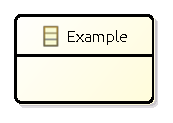
\includegraphics{images/05_library_of_transformations/02_type_level_transformations/01_regular_classes/class_type.pdf}
        \caption{$Tm_{Class}$ with $name = .\type{Example}$}
        \label{fig:library_of_transformations:type_level_transformations:regular_classes:visualisation:ecore}
    \end{subfigure}
    \begin{subfigure}{0.45\textwidth}
        \centering
        \input{images/05_library_of_transformations/02_type_level_transformations/01_regular_classes/class_as_node_type.tikz}
        \caption{$TG_{Class}$ with $name = .\type{Example}$}
        \label{fig:library_of_transformations:type_level_transformations:regular_classes:visualisation:groove}
    \end{subfigure}
    \caption{Visualisation of the transformation of regular classes}
    \label{fig:library_of_transformations:type_level_transformations:regular_classes:visualisation}
\end{figure}

The first transformation that will be defined is a transformation of regular classes. A class without any additional properties is considered a regular class. The Ecore model for defining a regular class is given in the following definition:

\begin{defin}[Type model $Tm_{Class}$]
\label{defin:library_of_transformations:type_level_transformations:regular_classes:tmod_class}
Let $Tm_{Class}$ be the type model containing a regular class with identifier $name$. $Tm_{Class}$ is defined as:
\begin{align*}
Class =\ &\{name\} \\
Enum =\ &\{\} \\
UserDataType =\ &\{\} \\
Field =\ &\{\} \\
\mathrm{FieldSig} =\ &\{\} \\
EnumValue =\ &\{\} \\
Inh =\ &\{\} \\
Prop =\ &\{\} \\
Constant =\ &\{\} \\
\mathrm{ConstType} =\ &\{\}
\end{align*}
\isabellelref{tmod_class}{Ecore-GROOVE-Mapping-Library.ClassType}
\end{defin}

\begin{thm}[Correctness of $Tm_{Class}$]
\label{defin:library_of_transformations:type_level_transformations:regular_classes:tmod_class_correct}
$Tm_{Class}$ (\cref{defin:library_of_transformations:type_level_transformations:regular_classes:tmod_class}) is a consistent type model in the sense of \cref{defin:formalisations:ecore_formalisation:type_models:type_model_consistency}.
\isabellelref{tmod_class_correct}{Ecore-GROOVE-Mapping-Library.ClassType}
\end{thm}

A visual representation of $Tm_{Class}$ with identifier $.\type{Example}$ can be seen in \cref{fig:library_of_transformations:type_level_transformations:regular_classes:visualisation:ecore}. The correctness proof of $Tm_{Class}$ is trivial, and therefore not included here. The proof can be found as part of the Isabelle validated proofs.

In order to make composing transformation functions possible, $Tm_{Class}$ should be compatible with the type model it is combined with.

\begin{thm}[Correctness of $\mathrm{combine}(Tm, Tm_{Class})$]
\label{defin:library_of_transformations:type_level_transformations:regular_classes:tmod_class_combine_correct}
Assume a type model $Tm$ that is consistent in the sense of \cref{defin:formalisations:ecore_formalisation:type_models:type_model_consistency}. Then $Tm$ is compatible with $Tm_{Class}$ (in the sense of \cref{defin:transformation_framework:type_models_and_type_graphs:combining_type_models:compatibility}) if:
\begin{itemize}
    \item The identifier of the class in $Tm_{Class}$ is not yet an identifier for a class, enumeration type or user-defined data type in $Tm$;
    \item The identifier of the class in $Tm_{Class}$ is not in the namespace of any class, enumeration type or user-defined data type in $Tm$;
    \item None of the identifiers in any class, enumeration type or user-defined data type in $Tm$ is in the namespace of the class in $Tm_{Class}$.
\end{itemize}
\isabellelref{tmod_class_combine_correct}{Ecore-GROOVE-Mapping-Library.ClassType}
\end{thm}

\begin{proof}
Use \cref{defin:transformation_framework:type_models_and_type_graphs:combining_type_models:tmod_combine_merge_correct}. It is possible to show that all assumptions hold. Now we have shown that $\mathrm{combine}(Tm, Tm_{Class})$ is consistent in the sense of \cref{defin:formalisations:ecore_formalisation:type_models:type_model_consistency}.
\end{proof}

The definitions and theorems for a regular class within Ecore are now complete. 

\subsubsection{Encoding as node type}

A possible encoding for regular classes in Ecore is using a node type in GROOVE. This node type will get a transformed identifier as name. The encoding corresponding to $Tm_{Class}$ can then be represented as $TG_{Class}$, defined in the following definition:

\begin{defin}[Type graph $TG_{Class}$]
\label{defin:library_of_transformations:type_level_transformations:regular_classes:tg_class_as_node_type}
Let $TG_{Class}$ be the type graph containing a single node type which encodes a regular class $name$. $TG_{Class}$ is defined as:
\begin{align*}
NT =\ &\{\mathrm{ns\_\!to\_\!list}(name)\} \\
ET =\ &\{\} \\
\!\!\sqsubseteq\ =\ &\{( \mathrm{ns\_\!to\_\!list}(name), \mathrm{ns\_\!to\_\!list}(name) )\} \\
abs =\ &\{\} \\
\mathrm{mult} =\ &\{\} \\
contains =\ &\{\}
\end{align*}
\isabellelref{tg_class_as_node_type}{Ecore-GROOVE-Mapping-Library.ClassType}
\end{defin}

\begin{thm}[Correctness of $TG_{Class}$]
\label{defin:library_of_transformations:type_level_transformations:regular_classes:tg_class_as_node_type_correct}
$TG_{Class}$ (\cref{defin:library_of_transformations:type_level_transformations:regular_classes:tg_class_as_node_type}) is a valid type graph in the sense of \cref{defin:formalisations:groove_formalisation:type_graphs:type_graph_validity}.
\isabellelref{tg_class_as_node_type_correct}{Ecore-GROOVE-Mapping-Library.ClassType}
\end{thm}

A visual representation of $TG_{Class}$ with identifier $.\type{Example}$ can be seen in \cref{fig:library_of_transformations:type_level_transformations:regular_classes:visualisation:groove}. The correctness proof of $TG_{Class}$ is trivial, and therefore not included here. The proof can be found as part of the Isabelle validated proofs.

In order to make composing transformation functions possible, $TG_{Class}$ should be compatible with the type graph it is combined with.

\begin{thm}[Correctness of $\mathrm{combine}(TG, TG_{Class})$]
\label{defin:library_of_transformations:type_level_transformations:regular_classes:tg_class_as_node_type_combine_correct}
Assume a type graph $TG$ that is valid in the sense of \cref{defin:formalisations:groove_formalisation:type_graphs:type_graph_validity}. Then $TG$ is compatible with $TG_{Class}$ (in the sense of \cref{defin:transformation_framework:type_models_and_type_graphs:combining_type_graphs:compatibility}) if:
\begin{itemize}
    \item The node type of the encoded class in $TG_{Class}$ is not a node type in $TG$.
\end{itemize}
\isabellelref{tg_class_as_node_type_combine_correct}{Ecore-GROOVE-Mapping-Library.ClassType}
\end{thm}

\begin{proof}
Use \cref{defin:transformation_framework:type_models_and_type_graphs:combining_type_graphs:tg_combine_merge_correct}. It is possible to show that all assumptions hold. Now we have shown that $\mathrm{combine}(TG, TG_{Class})$ is valid in the sense of \cref{defin:formalisations:groove_formalisation:type_graphs:type_graph_validity}.
\end{proof}

The next definitions define the transformation function from $Tm_{Class}$ to $TG_{Class}$:

\begin{defin}[Transformation function $f_{Class}$]
\label{defin:library_of_transformations:type_level_transformations:regular_classes:tmod_class_to_tg_class_as_node_type}
The transformation function $f_{Class}(Tm)$ is defined as:
\begin{align*}
NT =\ &\{\mathrm{ns\_\!to\_\!list}(c) \mid c \in Class_{Tm}\} \\
ET =\ &\{\} \\
\!\!\sqsubseteq\ =\ &\{( \mathrm{ns\_\!to\_\!list}(c_1), \mathrm{ns\_\!to\_\!list}(c_2) ) \mid c_1 \in Class_{Tm} \land c_2 \in Class_{Tm} \} \\
abs =\ &\{\} \\
\mathrm{mult} =\ &\{\} \\
contains =\ &\{\}
\end{align*}
\isabellelref{tmod_class_to_tg_class_as_node_type}{Ecore-GROOVE-Mapping-Library.ClassType}
\end{defin}

\begin{thm}[Correctness of $f_{Class}$]
\label{defin:library_of_transformations:type_level_transformations:regular_classes:tmod_class_to_tg_class_as_node_type_func}
$f_{Class}(Tm)$ (\cref{defin:library_of_transformations:type_level_transformations:regular_classes:tmod_class_to_tg_class_as_node_type}) is a valid transformation function in the sense of \cref{defin:transformation_framework:type_models_and_type_graphs:combining_transformation_functions:transformation_function_type_model_type_graph} transforming $Tm_{Class}$ into $TG_{Class}$.
\isabellelref{tmod_class_to_tg_class_as_node_type_func}{Ecore-GROOVE-Mapping-Library.ClassType}
\end{thm}

The proof of the correctness of $f_{Class}$ will not be included here. Instead, it can be found in the validated Isabelle theories.

Finally, to complete the transformation, the transformation function that transforms $TG_{Class}$ into $Tm_{Class}$ is defined:

\begin{defin}[Transformation function $f'_{Class}$]
\label{defin:library_of_transformations:type_level_transformations:regular_classes:tg_class_as_node_type_to_tmod_class}
The transformation function $f'_{Class}(TG)$ is defined as:
\begin{align*}
Class =\ &\{\mathrm{list\_\!to\_\!ns}(n) \mid n \in NT_{TG}\} \\
Enum =\ &\{\} \\
UserDataType =\ &\{\} \\
Field =\ &\{\} \\
\mathrm{FieldSig} =\ &\{\} \\
EnumValue =\ &\{\} \\
Inh =\ &\{\} \\
Prop =\ &\{\} \\
Constant =\ &\{\} \\
\mathrm{ConstType} =\ &\{\}
\end{align*}
\isabellelref{tg_class_as_node_type_to_tmod_class}{Ecore-GROOVE-Mapping-Library.ClassType}
\end{defin}

\begin{thm}[Correctness of $f'_{Class}$]
\label{defin:library_of_transformations:type_level_transformations:regular_classes:tg_class_as_node_type_to_tmod_class_func}
$f'_{Class}(TG)$ (\cref{defin:library_of_transformations:type_level_transformations:regular_classes:tg_class_as_node_type_to_tmod_class}) is a valid transformation function in the sense of \cref{defin:transformation_framework:type_models_and_type_graphs:combining_transformation_functions:transformation_function_type_graph_type_model} transforming $TG_{Class}$ into $Tm_{Class}$.
\isabellelref{tg_class_as_node_type_to_tmod_class_func}{Ecore-GROOVE-Mapping-Library.ClassType}
\end{thm}

Once more, the correctness proof is not included here but can be found in the validated Isabelle proofs of this thesis.
\subsection{Abstract classes}
\label{subsec:library_of_transformations:type_level_transformations:abstract_classes}

\begin{figure}[H]
    \centering
    \begin{subfigure}{0.45\textwidth}
        \centering
        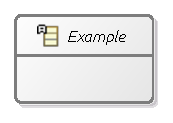
\includegraphics{images/05_library_of_transformations/02_type_level_transformations/02_abstract_classes/abstract_class_type.pdf}
        \caption{$Tm_{AbsClass}$ with $name = .\type{Example}$}
        \label{fig:library_of_transformations:type_level_transformations:abstract_classes:visualisation:ecore}
    \end{subfigure}
    \begin{subfigure}{0.45\textwidth}
        \centering
        \input{images/05_library_of_transformations/02_type_level_transformations/02_abstract_classes/abstract_class_as_node_type.tikz}
        \caption{$TG_{AbsClass}$ with $name = .\type{Example}$}
        \label{fig:library_of_transformations:type_level_transformations:abstract_classes:visualisation:groove}
    \end{subfigure}
    \caption{Visualisation of the transformation of abstract classes}
    \label{fig:library_of_transformations:type_level_transformations:abstract_classes:visualisation}
\end{figure}

This section defines a transformation that is very close to the previous transformation. In this section, an abstract class without any additional properties is defined. The Ecore model for defining an abstract class is given in the following definition:

\begin{defin}[Type model $Tm_{AbsClass}$]
\label{defin:library_of_transformations:type_level_transformations:abstract_classes:tmod_abstract_class}
Let $Tm_{AbsClass}$ be the type model containing an abstract class with identifier $name$. $Tm_{AbsClass}$ is defined as:
\begin{align*}
Class =\ &\{name\} \\
Enum =\ &\{\} \\
UserDataType =\ &\{\} \\
Field =\ &\{\} \\
\mathrm{FieldSig} =\ &\{\} \\
EnumValue =\ &\{\} \\
Inh =\ &\{\} \\
Prop =\ &\{[ \type{abstract}, name ]\} \\
Constant =\ &\{\} \\
\mathrm{ConstType} =\ &\{\}
\end{align*}
\isabellelref{tmod_abstract_class}{Ecore-GROOVE-Mapping-Library.AbstractClassType}
\end{defin}

\begin{thm}[Correctness of $Tm_{AbsClass}$]
\label{defin:library_of_transformations:type_level_transformations:abstract_classes:tmod_abstract_class_correct}
$Tm_{AbsClass}$ (\cref{defin:library_of_transformations:type_level_transformations:abstract_classes:tmod_abstract_class}) is a consistent type model in the sense of \cref{defin:formalisations:ecore_formalisation:type_models:type_model_consistency}.
\isabellelref{tmod_abstract_class_correct}{Ecore-GROOVE-Mapping-Library.AbstractClassType}
\end{thm}

A visual representation of $Tm_{AbsClass}$ with identifier $.\type{Example}$ can be seen in \cref{fig:library_of_transformations:type_level_transformations:abstract_classes:visualisation:ecore}. The correctness proof of $Tm_{AbsClass}$ is trivial, and therefore not included here. The proof can be found as part of the Isabelle validated proofs.

In order to make composing transformation functions possible, $Tm_{AbsClass}$ should be compatible with the type model it is combined with.

\begin{thm}[Correctness of $\mathrm{combine}(Tm, Tm_{AbsClass})$]
\label{defin:library_of_transformations:type_level_transformations:abstract_classes:tmod_abstract_class_combine_correct}
Assume a type model $Tm$ that is consistent in the sense of \cref{defin:formalisations:ecore_formalisation:type_models:type_model_consistency}. Then $Tm$ is compatible with $Tm_{AbsClass}$ (in the sense of \cref{defin:transformation_framework:type_models_and_type_graphs:combining_type_models:compatibility}) if:
\begin{itemize}
    \item The identifier of the class in $Tm_{AbsClass}$ is not yet an identifier for a class, enumeration type or user-defined data type in $Tm$;
    \item The identifier of the class in $Tm_{AbsClass}$ is not in the namespace of any class, enumeration type or user-defined data type in $Tm$;
    \item None of the identifiers in any class, enumeration type or user-defined data type in $Tm$ is in the namespace of the class in $Tm_{AbsClass}$.
\end{itemize}
\isabellelref{tmod_abstract_class_combine_correct}{Ecore-GROOVE-Mapping-Library.AbstractClassType}
\end{thm}

\begin{proof}
Use \cref{defin:transformation_framework:type_models_and_type_graphs:combining_type_models:tmod_combine_merge_correct}. It is possible to show that all assumptions hold. Now we have shown that $\mathrm{combine}(Tm, Tm_{AbsClass})$ is consistent in the sense of \cref{defin:formalisations:ecore_formalisation:type_models:type_model_consistency}.
\end{proof}

The definitions and theorems for a regular class within Ecore are now complete. 

\subsubsection{Encoding as node type}

A possible encoding for abstract classes in Ecore is using a node type in GROOVE. This node type will get a transformed identifier as name. The encoding corresponding to $Tm_{AbsClass}$ can then be represented as $TG_{AbsClass}$, defined in the following definition:

\begin{defin}[Type graph $TG_{AbsClass}$]
\label{defin:library_of_transformations:type_level_transformations:abstract_classes:tg_abstract_class_as_node_type}
Let $TG_{AbsClass}$ be the type graph containing a single node type which encodes an abstract class $name$. $TG_{AbsClass}$ is defined as:
\begin{align*}
NT =\ &\{\mathrm{ns\_\!to\_\!list}(name)\} \\
ET =\ &\{\} \\
\!\!\sqsubseteq\ =\ &\{(\mathrm{ns\_\!to\_\!list}(name), \mathrm{ns\_\!to\_\!list}(name))\} \\
abs =\ &\{\mathrm{ns\_\!to\_\!list}(name)\} \\
\mathrm{mult} =\ &\{\} \\
contains =\ &\{\}
\end{align*}
\isabellelref{tg_abstract_class_as_node_type}{Ecore-GROOVE-Mapping-Library.AbstractClassType}
\end{defin}

\begin{thm}[Correctness of $TG_{Class}$]
\label{defin:library_of_transformations:type_level_transformations:abstract_classes:tg_abstract_class_as_node_type_correct}
$TG_{AbsClass}$ (\cref{defin:library_of_transformations:type_level_transformations:abstract_classes:tg_abstract_class_as_node_type}) is a valid type graph in the sense of \cref{defin:formalisations:groove_formalisation:type_graphs:type_graph_validity}.
\isabellelref{tg_abstract_class_as_node_type_correct}{Ecore-GROOVE-Mapping-Library.AbstractClassType}
\end{thm}

A visual representation of $TG_{AbsClass}$ with identifier $.\type{Example}$ can be seen in \cref{fig:library_of_transformations:type_level_transformations:abstract_classes:visualisation:groove}. The correctness proof of $TG_{AbsClass}$ is trivial, and therefore not included here. The proof can be found as part of the Isabelle validated proofs.

In order to make composing transformation functions possible, $TG_{AbsClass}$ should be compatible with the type graph it is combined with.

\begin{thm}[Correctness of $\mathrm{combine}(TG, TG_{AbsClass})$]
\label{defin:library_of_transformations:type_level_transformations:abstract_classes:tg_abstract_class_as_node_type_combine_correct}
Assume a type graph $TG$ that is valid in the sense of \cref{defin:formalisations:groove_formalisation:type_graphs:type_graph_validity}. Then $TG$ is compatible with $TG_{AbsClass}$ (in the sense of \cref{defin:transformation_framework:type_models_and_type_graphs:combining_type_graphs:compatibility}) if:
\begin{itemize}
    \item The node type of the encoded class in $TG_{AbsClass}$ is not a node type in $TG$.
\end{itemize}
\isabellelref{tg_abstract_class_as_node_type_combine_correct}{Ecore-GROOVE-Mapping-Library.AbstractClassType}
\end{thm}

\begin{proof}
Use \cref{defin:transformation_framework:type_models_and_type_graphs:combining_type_graphs:tg_combine_merge_correct}. It is possible to show that all assumptions hold. Now we have shown that $\mathrm{combine}(TG, TG_{AbsClass})$ is valid in the sense of \cref{defin:formalisations:groove_formalisation:type_graphs:type_graph_validity}.
\end{proof}

The next definitions define the transformation function from $Tm_{AbsClass}$ to $TG_{AbsClass}$:

\begin{defin}[Transformation function $f_{AbsClass}$]
\label{defin:library_of_transformations:type_level_transformations:abstract_classes:tmod_abstract_class_to_tg_abstract_class_as_node_type}
The transformation function $f_{AbsClass}(Tm)$ is defined as:
\begin{align*}
NT =\ &\{\mathrm{ns\_\!to\_\!list}(c) \mid c \in Class_{Tm}\} \\
ET =\ &\{\} \\
\!\!\sqsubseteq\ =\ &\{(\mathrm{ns\_\!to\_\!list}(c_1), \mathrm{ns\_\!to\_\!list}(c_2)) \mid c_1 \in Class_{Tm} \land c_2 \in Class_{Tm} \} \\
abs =\ &\{\mathrm{ns\_\!to\_\!list}(c) \mid c \in Class_{Tm}\} \\
\mathrm{mult} =\ &\{\} \\
contains =\ &\{\}
\end{align*}
\isabellelref{tmod_abstract_class_to_tg_abstract_class_as_node_type}{Ecore-GROOVE-Mapping-Library.AbstractClassType}
\end{defin}

\begin{thm}[Correctness of $f_{AbsClass}$]
\label{defin:library_of_transformations:type_level_transformations:abstract_classes:tmod_abstract_class_to_tg_abstract_class_as_node_type_func}
$f_{AbsClass}(Tm)$ (\cref{defin:library_of_transformations:type_level_transformations:abstract_classes:tmod_abstract_class_to_tg_abstract_class_as_node_type}) is a valid transformation function in the sense of \cref{defin:transformation_framework:type_models_and_type_graphs:combining_transformation_functions:transformation_function_type_model_type_graph} transforming $Tm_{AbsClass}$ into $TG_{AbsClass}$.
\isabellelref{tmod_abstract_class_to_tg_abstract_class_as_node_type_func}{Ecore-GROOVE-Mapping-Library.AbstractClassType}
\end{thm}

The proof of the correctness of $f_{AbsClass}$ will not be included here. Instead, it can be found in the validated Isabelle theories.

Finally, to complete the transformation, the transformation function that transforms $TG_{AbsClass}$ into $Tm_{AbsClass}$ is defined:

\begin{defin}[Transformation function $f'_{AbsClass}$]
\label{defin:library_of_transformations:type_level_transformations:abstract_classes:tg_abstract_class_as_node_type_to_tmod_abstract_class}
The transformation function $f'_{AbsClass}(TG)$ is defined as:
\begin{align*}
Class =\ &\{\mathrm{list\_\!to\_\!ns}(n) \mid n \in NT_{TG}\} \\
Enum =\ &\{\} \\
UserDataType =\ &\{\} \\
Field =\ &\{\} \\
\mathrm{FieldSig} =\ &\{\} \\
EnumValue =\ &\{\} \\
Inh =\ &\{\} \\
Prop =\ &\{[ \type{abstract}, \mathrm{ns\_\!to\_\!list}(c) ] \mid c \in Class_{Tm}\} \\
Constant =\ &\{\} \\
\mathrm{ConstType} =\ &\{\}
\end{align*}
\isabellelref{tg_abstract_class_as_node_type_to_tmod_abstract_class}{Ecore-GROOVE-Mapping-Library.AbstractClassType}
\end{defin}

\begin{thm}[Correctness of $f'_{AbsClass}$]
\label{defin:library_of_transformations:type_level_transformations:abstract_classes:tg_abstract_class_as_node_type_to_tmod_abstract_class_func}
$f'_{AbsClass}(TG)$ (\cref{defin:library_of_transformations:type_level_transformations:abstract_classes:tg_abstract_class_as_node_type_to_tmod_abstract_class}) is a valid transformation function in the sense of \cref{defin:transformation_framework:type_models_and_type_graphs:combining_transformation_functions:transformation_function_type_graph_type_model} transforming $TG_{AbsClass}$ into $Tm_{AbsClass}$.
\isabellelref{tg_abstract_class_as_node_type_to_tmod_abstract_class_func}{Ecore-GROOVE-Mapping-Library.AbstractClassType}
\end{thm}

Once more, the correctness proof is not included here but can be found in the validated Isabelle proofs of this thesis.
\subsection{Regular subclasses}
\label{subsec:library_of_transformations:type_level_transformations:regular_subclasses}

\begin{figure}[H]
    \centering
    \begin{subfigure}{0.4\textwidth}
        \centering
        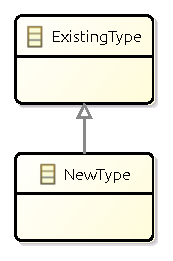
\includegraphics{images/05_library_of_transformations/02_type_level_transformations/03_regular_subclasses/class_subtype.pdf}
        \caption{$Tm_{Subclass}$ with $name = .\type{NewType}$ and $supertype = .\type{ExistingType}$}
        \label{fig:library_of_transformations:type_level_transformations:regular_subclasses:visualisation:ecore}
    \end{subfigure}
    \begin{subfigure}{0.4\textwidth}
        \centering
        \input{images/05_library_of_transformations/02_type_level_transformations/03_regular_subclasses/subclass_as_node_type.tikz}
        \caption{$TG_{Subclass}$ with $name = .\type{NewType}$ and $supertype = .\type{ExistingType}$}
        \label{fig:library_of_transformations:type_level_transformations:regular_subclasses:visualisation:groove}
    \end{subfigure}
    \caption{Visualisation of the transformation of regular subclasses}
    \label{fig:library_of_transformations:type_level_transformations:regular_subclasses:visualisation}
\end{figure}

This section will define the transformation of a regular subclass. Within this transformation, a newly introduced subclass is transformed, which extends an existing supertype. The Ecore type model that introduces such a subclass is defined as follows:

\begin{defin}[Type model $Tm_{Subclass}$]
\label{defin:library_of_transformations:type_level_transformations:regular_subclasses:tmod_subclass}
Let $Tm_{Subclass}$ be the type model containing a regular class with identifier $name$. The regular class $name$ extends another regular class with identifier $supertype$. Furthermore, $name \neq supertype$. $Tm_{Subclass}$ is defined as:
\begin{align*}
Class =\ &\{name, supertype\} \\
Enum =\ &\{\} \\
UserDataType =\ &\{\} \\
Field =\ &\{\} \\
\mathrm{FieldSig} =\ &\{\} \\
EnumValue =\ &\{\} \\
Inh =\ &\{(name, supertype)\} \\
Prop =\ &\{\} \\
Constant =\ &\{\} \\
\mathrm{ConstType} =\ &\{\}
\end{align*}
\isabellelref{tmod_subclass}{Ecore-GROOVE-Mapping-Library.SubclassType}
\end{defin}

\begin{thm}[Correctness of $Tm_{Subclass}$]
\label{defin:library_of_transformations:type_level_transformations:regular_subclasses:tmod_subclass_correct}
$Tm_{Subclass}$ (\cref{defin:library_of_transformations:type_level_transformations:regular_subclasses:tmod_subclass}) is a consistent type model in the sense of \cref{defin:formalisations:ecore_formalisation:type_models:type_model_consistency}.
\isabellelref{tmod_subclass_correct}{Ecore-GROOVE-Mapping-Library.SubclassType}
\end{thm}

A visual representation of $Tm_{Subclass}$ with the new subclass identified as $.\type{NewType}$ and the existing supertype identified as $.\type{ExistingType}$ can be seen in \cref{fig:library_of_transformations:type_level_transformations:regular_subclasses:visualisation:ecore}. The correctness proof of $Tm_{Subclass}$ is trivial, and therefore not included here. The proof can be found as part of the Isabelle validated proofs.

In order to make composing transformation functions possible, $Tm_{Subclass}$ should be compatible with the type model it is combined with.

\begin{thm}[Correctness of $\mathrm{combine}(Tm, Tm_{Subclass})$]
\label{defin:library_of_transformations:type_level_transformations:regular_subclasses:tmod_subclass_combine_correct}
Assume a type model $Tm$ that is consistent in the sense of \cref{defin:formalisations:ecore_formalisation:type_models:type_model_consistency}. Then $Tm$ is compatible with $Tm_{Subclass}$ (in the sense of \cref{defin:transformation_framework:type_models_and_type_graphs:combining_type_models:compatibility}) if:
\begin{itemize}
    \item The only shared type is the supertype, so $Class_{Tm} \cap Class_{Tm_{Subclass}} = \{ supertype \}$;
    \item The class $name$ is not in the namespace of class $supertype$, and vice versa;
    \item $name$ is not used as an identifier for an enumeration type or user-defined data type in $Tm$;
    \item The identifier of the class $name$ in $Tm_{Class}$ is not in the namespace of any class, enumeration type or user-defined data type in $Tm$;
    \item None of the identifiers in any class, enumeration type or user-defined data type in $Tm$ is in the namespace of the class $name$ in $Tm_{Class}$.
\end{itemize}
\isabellelref{tmod_subclass_combine_correct}{Ecore-GROOVE-Mapping-Library.SubclassType}
\end{thm}

\begin{proof}
Use \cref{defin:transformation_framework:type_models_and_type_graphs:combining_type_models:tmod_combine_merge_correct}. It is possible to show that all assumptions hold. For proving that the transitive closure of the inheritance relation is irreflexive, use the fact that $name$ only appears in the domain of the relation. Now we have shown that $\mathrm{combine}(Tm, Tm_{Class})$ is consistent in the sense of \cref{defin:formalisations:ecore_formalisation:type_models:type_model_consistency}.
\end{proof}

The definitions and theorems for a regular subclass within Ecore are now complete. 

\subsubsection{Encoding as node type}

A possible encoding for regular subclasses in Ecore is using node types in GROOVE. The supertype and newly introduced subtype will both be node types with their corresponding identifiers transformed. The encoding corresponding to $Tm_{Subclass}$ can then be represented as $TG_{Subclass}$, defined in the following definition:

\begin{defin}[Type graph $TG_{Subclass}$]
\label{defin:library_of_transformations:type_level_transformations:regular_subclasses:tg_subclass_as_node_type}
Let $TG_{Subclass}$ be a type graph containing a two node types. The first node type encodes the regular class $supertype$. The second node type encodes a regular class $name$ which extends the encoded class $supertype$. Furthermore $name \neq supertype$. $TG_{Subclass}$ is defined as:
\begin{align*}
NT =\ &\{\mathrm{ns\_\!to\_\!list}(name), \mathrm{ns\_\!to\_\!list}(supertype)\} \\
ET =\ &\{\} \\
\!\!\sqsubseteq\ =\ &\{
(\mathrm{ns\_\!to\_\!list}(name), \mathrm{ns\_\!to\_\!list}(name)), \\&
(\mathrm{ns\_\!to\_\!list}(supertype), \mathrm{ns\_\!to\_\!list}(supertype)), \\&
(\mathrm{ns\_\!to\_\!list}(name), \mathrm{ns\_\!to\_\!list}(supertype))
\} \\
abs =\ &\{\} \\
\mathrm{mult} =\ &\{\} \\
contains =\ &\{\}
\end{align*}
\isabellelref{tg_subclass_as_node_type}{Ecore-GROOVE-Mapping-Library.SubclassType}
\end{defin}

\begin{thm}[Correctness of $TG_{Subclass}$]
\label{defin:library_of_transformations:type_level_transformations:regular_subclasses:tg_subclass_as_node_type_correct}
$TG_{Subclass}$ (\cref{defin:library_of_transformations:type_level_transformations:regular_subclasses:tg_subclass_as_node_type}) is a valid type graph in the sense of \cref{defin:formalisations:groove_formalisation:type_graphs:type_graph_validity}.
\isabellelref{tg_subclass_as_node_type_correct}{Ecore-GROOVE-Mapping-Library.SubclassType}
\end{thm}

A visual representation of $TG_{Subclass}$ with the new subclass identified as $.\type{NewType}$ and the existing supertype identified as $.\type{ExistingType}$ both encoded as node type, is shown in \cref{fig:library_of_transformations:type_level_transformations:regular_subclasses:visualisation:groove}. The correctness proof of $TG_{Subclass}$ is trivial, and therefore not included here. The proof can be found as part of the Isabelle validated proofs.

In order to make composing transformation functions possible, $TG_{Subclass}$ should be compatible with the type graph it is combined with.

\begin{thm}[Correctness of $\mathrm{combine}(TG, TG_{Subclass})$]
\label{defin:library_of_transformations:type_level_transformations:regular_subclasses:tg_subclass_as_node_type_combine_correct}
Assume a type graph $TG$ that is valid in the sense of \cref{defin:formalisations:groove_formalisation:type_graphs:type_graph_validity}. Then $TG$ is compatible with $TG_{Subclass}$ (in the sense of \cref{defin:transformation_framework:type_models_and_type_graphs:combining_type_graphs:compatibility}) if:
\begin{itemize}
    \item The only shared node type in $TG$ and $TG_{Subclass}$ is the node type of the encoded supertype.
\end{itemize}
\isabellelref{tg_subclass_as_node_type_combine_correct}{Ecore-GROOVE-Mapping-Library.SubclassType}
\end{thm}

\begin{proof}
Use \cref{defin:transformation_framework:type_models_and_type_graphs:combining_type_graphs:tg_combine_merge_correct}. It is possible to show that all assumptions hold. For proving the antisymmetry of the inheritance relation, use the fact that the node type which encodes class $name$ only appears in the domain of the relation. Now we have shown that $\mathrm{combine}(TG, TG_{Subclass})$ is valid in the sense of \cref{defin:formalisations:groove_formalisation:type_graphs:type_graph_validity}.
\end{proof}

The next definitions define the transformation function from $Tm_{Sublass}$ to $TG_{Sublass}$:

\begin{defin}[Transformation function $f_{Subclass}$]
\label{defin:library_of_transformations:type_level_transformations:regular_subclasses:tmod_subclass_to_tg_subclass_as_node_type}
The transformation function $f_{Subclass}(Tm)$ is defined as:
\begin{align*}
NT =\ &\{\mathrm{ns\_\!to\_\!list}(c) \mid c \in Class_{Tm}\} \\
ET =\ &\{\} \\
\!\!\sqsubseteq\ =\ &\{(\mathrm{ns\_\!to\_\!list}(c_1), \mathrm{ns\_\!to\_\!list}(c_2)) \mid c_1 \in Class_{Tm} \land c_2 \in Class_{Tm} \land c_1 = c_2 \}\ \cup \\&
\{(\mathrm{ns\_\!to\_\!list}(i), \mathrm{ns\_\!to\_\!list}(j)) \mid (i, j) \in Inh_{Tm} \} \\
abs =\ &\{\} \\
\mathrm{mult} =\ &\{\} \\
contains =\ &\{\}
\end{align*}
\isabellelref{tmod_subclass_to_tg_subclass_as_node_type}{Ecore-GROOVE-Mapping-Library.SubclassType}
\end{defin}

\begin{thm}[Correctness of $f_{Subclass}$]
\label{defin:library_of_transformations:type_level_transformations:regular_subclasses:tmod_subclass_to_tg_subclass_as_node_type_func}
$f_{Subclass}(Tm)$ (\cref{defin:library_of_transformations:type_level_transformations:regular_subclasses:tmod_subclass_to_tg_subclass_as_node_type}) is a valid transformation function in the sense of \cref{defin:transformation_framework:type_models_and_type_graphs:combining_transformation_functions:transformation_function_type_model_type_graph} transforming $Tm_{Subclass}$ into $TG_{Subclass}$.
\isabellelref{tmod_subclass_to_tg_subclass_as_node_type_func}{Ecore-GROOVE-Mapping-Library.SubclassType}
\end{thm}

The proof of the correctness of $f_{Subclass}$ will not be included here. Instead, it can be found in the validated Isabelle theories.

Finally, to complete the transformation, the transformation function that transforms $TG_{Subclass}$ into $Tm_{Subclass}$ is defined:

\begin{defin}[Transformation function $f'_{Subclass}$]
\label{defin:library_of_transformations:type_level_transformations:regular_subclasses:tg_subclass_as_node_type_to_tmod_subclass}
The transformation function $f'_{Subclass}(TG)$ is defined as:
\begin{align*}
Class =\ &\{\mathrm{list\_\!to\_\!ns}(n) \mid n \in NT_{TG}\} \\
Enum =\ &\{\} \\
UserDataType =\ &\{\} \\
Field =\ &\{\} \\
\mathrm{FieldSig} =\ &\{\} \\
EnumValue =\ &\{\} \\
Inh =\ &\{(\mathrm{list\_\!to\_\!ns}(i), \mathrm{list\_\!to\_\!ns}(j)) \mid (i, j) \in\ \sqsubseteq_{TG} \land\ i \neq j \} \\
Prop =\ &\{\} \\
Constant =\ &\{\} \\
\mathrm{ConstType} =\ &\{\}
\end{align*}
\isabellelref{tg_subclass_as_node_type_to_tmod_subclass}{Ecore-GROOVE-Mapping-Library.SubclassType}
\end{defin}

\begin{thm}[Correctness of $f'_{Subclass}$]
\label{defin:library_of_transformations:type_level_transformations:regular_subclasses:tg_subclass_as_node_type_to_tmod_subclass_func}
$f'_{Subclass}(TG)$ (\cref{defin:library_of_transformations:type_level_transformations:regular_subclasses:tg_subclass_as_node_type_to_tmod_subclass}) is a valid transformation function in the sense of \cref{defin:transformation_framework:type_models_and_type_graphs:combining_transformation_functions:transformation_function_type_graph_type_model} transforming $TG_{Subclass}$ into $Tm_{Subclass}$.
\isabellelref{tg_subclass_as_node_type_to_tmod_subclass_func}{Ecore-GROOVE-Mapping-Library.SubclassType}
\end{thm}

Once more, the correctness proof is not included here but can be found in the validated Isabelle proofs of this thesis.
\subsection{Enumeration types}
\label{subsec:library_of_transformations:type_level_transformations:enumeration_types}

\begin{figure}[H]
    \centering
    \begin{subfigure}{0.25\textwidth}
        \centering
        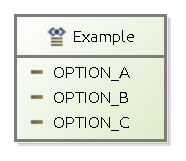
\includegraphics{images/05_library_of_transformations/02_type_level_transformations/04_enumeration_types/enum_type.pdf}
        \caption{$Tm_{Enum}$ with \\$name = .\type{Example}$ and \\$values = \{ \type{OPTION\_A},$\\$ \type{OPTION\_B}, \type{OPTION\_C} \}$}
        \label{fig:library_of_transformations:type_level_transformations:enumeration_types:visualisation:ecore}
    \end{subfigure}
    \\
    \begin{subfigure}{0.65\textwidth}
        \centering
        \input{images/05_library_of_transformations/02_type_level_transformations/04_enumeration_types/enum_as_node_types.tikz}
        \caption{$TG_{EnumNodes}$ with $name = .\type{Example}$ and\\$values = \{ \type{OPTION\_A}, \type{OPTION\_B}, \type{OPTION\_C} \}$}
        \label{fig:library_of_transformations:type_level_transformations:enumeration_types:visualisation:groove_nodes}
    \end{subfigure}
    \begin{subfigure}{0.25\textwidth}
        \centering
        \input{images/05_library_of_transformations/02_type_level_transformations/04_enumeration_types/enum_as_flags.tikz}
        \caption{$TG_{EnumFlags}$ with \\$name = .\type{Example}$ and \\$values = \{ \type{OPTION\_A},$\\$ \type{OPTION\_B}, \type{OPTION\_C} \}$}
        \label{fig:library_of_transformations:type_level_transformations:enumeration_types:visualisation:groove_flags}
    \end{subfigure}
    \caption{Visualisations of the transformations of enumeration types}
    \label{fig:library_of_transformations:type_level_transformations:enumeration_types:visualisation}
\end{figure}

This section will define the transformation of an enumeration type. Within this transformation, a new enumeration type is introduced, including its possible values. The Ecore type model that introduces such a subclass is defined as follows:

\begin{defin}[Type model $Tm_{Enum}$]
\label{defin:library_of_transformations:type_level_transformations:enumeration_types:tmod_enum}
Let $Tm_{Enum}$ be the type model containing a enumeration type with identifier $name$. The values of this enumeration type are defined as part of sequence $values$. $Tm_{Enum}$ is defined as:
\begin{align*}
Class =\ &\{\} \\
Enum =\ &\{name\} \\
UserDataType =\ &\{\} \\
Field =\ &\{\} \\
\mathrm{FieldSig} =\ &\{\} \\
EnumValue =\ &\{ (name, v) \mid v \in values \} \\
Inh =\ &\{\} \\
Prop =\ &\{\} \\
Constant =\ &\{\} \\
\mathrm{ConstType} =\ &\{\}
\end{align*}
\isabellelref{tmod_enum}{Ecore-GROOVE-Mapping-Library.EnumType}
\end{defin}

\begin{thm}[Correctness of $Tm_{Enum}$]
\label{defin:library_of_transformations:type_level_transformations:enumeration_types:tmod_enum_correct}
$Tm_{Subclass}$ (\cref{defin:library_of_transformations:type_level_transformations:enumeration_types:tmod_enum}) is a consistent type model in the sense of \cref{defin:formalisations:ecore_formalisation:type_models:type_model_consistency}.
\isabellelref{tmod_enum_correct}{Ecore-GROOVE-Mapping-Library.EnumType}
\end{thm}

A visual representation of $Tm_{Enum}$ with $.\type{Example}$ as identifier for the new enumeration type and $\type{OPTION\_A}$, $\type{OPTION\_B}$ and $\type{OPTION\_C}$ as its values can be seen in \cref{fig:library_of_transformations:type_level_transformations:enumeration_types:visualisation:ecore}. The correctness proof of $Tm_{Enum}$ is trivial, and therefore not included here. The proof can be found as part of the Isabelle validated proofs.

In order to make composing transformation functions possible, $Tm_{Enum}$ should be compatible with the type model it is combined with.

\begin{thm}[Correctness of $\mathrm{combine}(Tm, Tm_{Enum})$]
\label{defin:library_of_transformations:type_level_transformations:enumeration_types:tmod_enum_combine_correct}
Assume a type model $Tm$ that is consistent in the sense of \cref{defin:formalisations:ecore_formalisation:type_models:type_model_consistency}. Then $Tm$ is compatible with $Tm_{Enum}$ (in the sense of \cref{defin:transformation_framework:type_models_and_type_graphs:combining_type_models:compatibility}) if:
\begin{itemize}
    \item The identifier of the enumeration type in $Tm_{Enum}$ is not yet an identifier for a class, enumeration type or user-defined data type in $Tm$;
    \item The identifier of the enumeration type in $Tm_{Enum}$ is not in the namespace of any class, enumeration type or user-defined data type in $Tm$;
    \item None of the identifiers in any class, enumeration type or user-defined data type in $Tm$ is in the namespace of the enumeration type in $Tm_{Enum}$.
\end{itemize}
\isabellelref{tmod_enum_combine_correct}{Ecore-GROOVE-Mapping-Library.EnumType}
\end{thm}

\begin{proof}
Use \cref{defin:transformation_framework:type_models_and_type_graphs:combining_type_models:tmod_combine_merge_correct}. It is possible to show that all assumptions hold. Now we have shown that $\mathrm{combine}(Tm, Tm_{Enum})$ is consistent in the sense of \cref{defin:formalisations:ecore_formalisation:type_models:type_model_consistency}.
\end{proof}

The definitions and theorems for a regular subclass within Ecore are now complete. 

\subsubsection{Encoding as node type}

A possible encoding for enumeration types in Ecore is using node types in GROOVE. In this case, the enumeration type itself is transformed into an abstract node type. Each value of the enumeration type is converted to its own node type, extending the abstract node type. The encoding corresponding to $Tm_{Enum}$ can then be represented as $TG_{EnumNodes}$, defined in the following definition:

\begin{defin}[Type graph $TG_{EnumNodes}$]
\label{defin:library_of_transformations:type_level_transformations:enumeration_types:tg_enum_as_node_types}
Let $TG_{EnumNodes}$ be a type graph containing multiple node types. The first node type encodes the enumeration type $name$. The other node types encode the $values$ of enumeration type $name$. $TG_{EnumNodes}$ is defined as:
\begin{align*}
NT =\ &\{\mathrm{ns\_\!to\_\!list}(name)\} \cup \{ \mathrm{ns\_\!to\_\!list}(name) \append \langle v \rangle \mid v \in values \} \\
ET =\ &\{\} \\
\!\!\sqsubseteq\ =\ &\{(\mathrm{ns\_\!to\_\!list}(name), \mathrm{ns\_\!to\_\!list}(name))\}\ \cup \\&
\{(\mathrm{ns\_\!to\_\!list}(name) \append \langle v \rangle, \mathrm{ns\_\!to\_\!list}(name) \append \langle v \rangle) \mid v \in values \}\ \cup \\&
\{(\mathrm{ns\_\!to\_\!list}(name) \append \langle v \rangle, \mathrm{ns\_\!to\_\!list}(name)) \mid v \in values \} \\
abs =\ &\{\mathrm{ns\_\!to\_\!list}(name)\} \\
\mathrm{mult} =\ &\{\} \\
contains =\ &\{\}
\end{align*}
\isabellelref{tg_enum_as_node_types}{Ecore-GROOVE-Mapping-Library.EnumType}
\end{defin}

\begin{thm}[Correctness of $TG_{EnumNodes}$]
\label{defin:library_of_transformations:type_level_transformations:enumeration_types:tg_enum_as_node_types_correct}
$TG_{EnumNodes}$ (\cref{defin:library_of_transformations:type_level_transformations:enumeration_types:tg_enum_as_node_types}) is a valid type graph in the sense of \cref{defin:formalisations:groove_formalisation:type_graphs:type_graph_validity}.
\isabellelref{tg_enum_as_node_types_correct}{Ecore-GROOVE-Mapping-Library.EnumType}
\end{thm}

A visual representation of $TG_{EnumNodes}$ with $.\type{Example}$ as identifier for the encoded enumeration type and $\type{OPTION\_A}$, $\type{OPTION\_B}$ and $\type{OPTION\_C}$ as its values can be seen in \cref{fig:library_of_transformations:type_level_transformations:enumeration_types:visualisation:groove_nodes}. Please note that in this visualisation, the sequences are concatenated using the dollar sign $\$$. The correctness proof of $TG_{EnumNodes}$ is trivial, and therefore not included here. The proof can be found as part of the Isabelle validated proofs.

In order to make composing transformation functions possible, $TG_{EnumNodes}$ should be compatible with the type graph it is combined with.

\begin{thm}[Correctness of $\mathrm{combine}(TG, TG_{EnumNodes})$]
\label{defin:library_of_transformations:type_level_transformations:enumeration_types:tg_enum_as_node_types_combine_correct}
Assume a type graph $TG$ that is valid in the sense of \cref{defin:formalisations:groove_formalisation:type_graphs:type_graph_validity}. Then $TG$ is compatible with $TG_{EnumNodes}$ (in the sense of \cref{defin:transformation_framework:type_models_and_type_graphs:combining_type_graphs:compatibility}) if:
\begin{itemize}
    \item There are no shared node types between $TG_{EnumNodes}$ and $TG$.
\end{itemize}
\isabellelref{tg_enum_as_node_types_combine_correct}{Ecore-GROOVE-Mapping-Library.EnumType}
\end{thm}

\begin{proof}
Use \cref{defin:transformation_framework:type_models_and_type_graphs:combining_type_graphs:tg_combine_merge_correct}. It is possible to show that all assumptions hold. Now we have shown that $\mathrm{combine}(TG, TG_{EnumNodes})$ is valid in the sense of \cref{defin:formalisations:groove_formalisation:type_graphs:type_graph_validity}.
\end{proof}

The next definitions define the transformation function from $Tm_{Enum}$ to $TG_{EnumNodes}$:

\begin{defin}[Transformation function $f_{EnumNodes}$]
\label{defin:library_of_transformations:type_level_transformations:enumeration_types:tmod_enum_to_tg_enum_as_node_types}
The transformation function $f_{EnumNodes}(Tm)$ is defined as:
\begin{align*}
NT =\ &\{\mathrm{ns\_\!to\_\!list}(e) \mid e \in Enum_{Tm}\} \cup \{\mathrm{ns\_\!to\_\!list}(e) \append \langle v \rangle \mid (e, v) \in EnumValue_{Tm}\} \\
ET =\ &\{\} \\
\!\!\sqsubseteq\ =\ &\{(\mathrm{ns\_\!to\_\!list}(e_1), \mathrm{ns\_\!to\_\!list}(e_2)) \mid e_1 \in Enum_{Tm} \land e_2 \in Enum_{Tm} \}\ \cup \\&
\{(\mathrm{ns\_\!to\_\!list}(i) \append \langle j \rangle, \mathrm{ns\_\!to\_\!list}(i) \append \langle j \rangle) \mid (i, j) \in EnumValue_{Tm} \}\ \cup \\&
\{(\mathrm{ns\_\!to\_\!list}(i) \append \langle j \rangle, \mathrm{ns\_\!to\_\!list}(e)) \mid (i, j) \in EnumValue_{Tm} \land e \in Enum_{Tm} \} \\
abs =\ &\{\} \\
\mathrm{mult} =\ &\{\} \\
contains =\ &\{\}
\end{align*}
\isabellelref{tmod_enum_to_tg_enum_as_node_types}{Ecore-GROOVE-Mapping-Library.EnumType}
\end{defin}

\begin{thm}[Correctness of $f_{EnumNodes}$]
\label{defin:library_of_transformations:type_level_transformations:enumeration_types:tmod_enum_to_tg_enum_as_node_types_func}
$f_{EnumNodes}(Tm)$ (\cref{defin:library_of_transformations:type_level_transformations:enumeration_types:tmod_enum_to_tg_enum_as_node_types}) is a valid transformation function in the sense of \cref{defin:transformation_framework:type_models_and_type_graphs:combining_transformation_functions:transformation_function_type_model_type_graph} transforming $Tm_{Enum}$ into $TG_{EnumNodes}$.
\isabellelref{tmod_enum_to_tg_enum_as_node_types_func}{Ecore-GROOVE-Mapping-Library.EnumType}
\end{thm}

The proof of the correctness of $f_{EnumNodes}$ will not be included here. Instead, it can be found in the validated Isabelle theories.

Finally, to complete the transformation, the transformation function that transforms $TG_{EnumNodes}$ into $Tm_{Enum}$ is defined:

\begin{defin}[Transformation function $f'_{EnumNodes}$]
\label{defin:library_of_transformations:type_level_transformations:enumeration_types:tg_enum_as_node_types_to_tmod_enum}
The transformation function $f'_{EnumNodes}(TG, name)$ is defined as:
\begin{align*}
Class =\ &\{\} \\
Enum =\ &\{\mathrm{list\_\!to\_\!ns}(n) \mid n \in NT_{TG} \land n = \mathrm{id\_\!to\_\!name}(name)\} \\
UserDataType =\ &\{\} \\
Field =\ &\{\} \\
\mathrm{FieldSig} =\ &\{\} \\
EnumValue =\ &\{(\mathrm{list\_\!to\_\!ns}(e), v) \mid e \append \langle v \rangle \in NT_{TG} \land e \append \langle v \rangle \neq \mathrm{id\_\!to\_\!name}(name) \} \\
Inh =\ &\{\} \\
Prop =\ &\{\} \\
Constant =\ &\{\} \\
\mathrm{ConstType} =\ &\{\}
\end{align*}
\isabellelref{tg_enum_as_node_types_to_tmod_enum}{Ecore-GROOVE-Mapping-Library.EnumType}
\end{defin}

\begin{thm}[Correctness of $f'_{EnumNodes}$]
\label{defin:library_of_transformations:type_level_transformations:enumeration_types:tg_enum_as_node_types_to_tmod_enum_func}
$f'_{EnumNodes}(TG, name)$ (\cref{defin:library_of_transformations:type_level_transformations:enumeration_types:tg_enum_as_node_types_to_tmod_enum}) is a valid transformation function in the sense of \cref{defin:transformation_framework:type_models_and_type_graphs:combining_transformation_functions:transformation_function_type_graph_type_model} transforming $TG_{EnumNodes}$ into $Tm_{Enum}$.
\isabellelref{tg_enum_as_node_types_to_tmod_enum_func}{Ecore-GROOVE-Mapping-Library.EnumType}
\end{thm}

Once more, the correctness proof is not included here but can be found in the validated Isabelle proofs of this thesis.

\subsubsection{Encoding as flags}

Another possible encoding for enumeration types in Ecore is using flags in GROOVE. In this case, the enumeration type itself is transformed into a regular node type. Each value of the enumeration type is converted to a flag on this node type. The encoding corresponding to $Tm_{Enum}$ can then be represented as $TG_{EnumFlags}$, defined in the following definition:

\begin{defin}[Type graph $TG_{EnumFlags}$]
\label{defin:library_of_transformations:type_level_transformations:enumeration_types:tg_enum_as_flags}
Let $TG_{EnumFlags}$ be a type graph containing a single node type which encodes the enumeration type $name$. The flags on the node type of $name$ encode the different $values$. $TG_{EnumFlags}$ is defined as:
\begin{align*}
NT =\ &\{\mathrm{ns\_\!to\_\!list}(name)\} \\
ET =\ &\{ (\mathrm{ns\_\!to\_\!list}(name), \langle v \rangle, \mathrm{ns\_\!to\_\!list}(name)) \mid v \in values \}\\
\!\!\sqsubseteq\ =\ &\{(\mathrm{ns\_\!to\_\!list}(name), \mathrm{ns\_\!to\_\!list}(name))\} \\
abs =\ &\{\} \\
\mathrm{mult}(e) =\ &\begin{cases}
    (0..1, 0..1) &\mathrm{if}\ e \in ET_{TG_{EnumFlags}}
\end{cases}\\
contains =\ &\{\}
\end{align*}
\isabellelref{tg_enum_as_flags}{Ecore-GROOVE-Mapping-Library.EnumType}
\end{defin}

\begin{thm}[Correctness of $TG_{EnumFlags}$]
\label{defin:library_of_transformations:type_level_transformations:enumeration_types:tg_enum_as_flags_correct}
$TG_{EnumFlags}$ (\cref{defin:library_of_transformations:type_level_transformations:enumeration_types:tg_enum_as_flags}) is a valid type graph in the sense of \cref{defin:formalisations:groove_formalisation:type_graphs:type_graph_validity}.
\isabellelref{tg_enum_as_flags_correct}{Ecore-GROOVE-Mapping-Library.EnumType}
\end{thm}

A visual representation of $TG_{EnumFlags}$ with $.\type{Example}$ as identifier for the encoded enumeration type and $\type{OPTION\_A}$, $\type{OPTION\_B}$ and $\type{OPTION\_C}$ as its values can be seen in \cref{fig:library_of_transformations:type_level_transformations:enumeration_types:visualisation:groove_flags}. The correctness proof of $TG_{EnumFlags}$ is trivial, and therefore not included here. The proof can be found as part of the Isabelle validated proofs.

In order to make composing transformation functions possible, $TG_{EnumFlags}$ should be compatible with the type graph it is combined with.

\begin{thm}[Correctness of $\mathrm{combine}(TG, TG_{EnumFlags})$]
\label{defin:library_of_transformations:type_level_transformations:enumeration_types:tg_enum_as_flags_combine_correct}
Assume a type graph $TG$ that is valid in the sense of \cref{defin:formalisations:groove_formalisation:type_graphs:type_graph_validity}. Then $TG$ is compatible with $TG_{EnumFlags}$ (in the sense of \cref{defin:transformation_framework:type_models_and_type_graphs:combining_type_graphs:compatibility}) if:
\begin{itemize}
    \item There are no shared node types between $TG_{EnumFlags}$ and $TG$.
\end{itemize}
\isabellelref{tg_enum_as_flags_combine_correct}{Ecore-GROOVE-Mapping-Library.EnumType}
\end{thm}

\begin{proof}
Use \cref{defin:transformation_framework:type_models_and_type_graphs:combining_type_graphs:tg_combine_merge_correct}. It is possible to show that all assumptions hold. Now we have shown that $\mathrm{combine}(TG, TG_{EnumFlags})$ is valid in the sense of \cref{defin:formalisations:groove_formalisation:type_graphs:type_graph_validity}.
\end{proof}

The next definitions define the transformation function from $Tm_{Enum}$ to $TG_{EnumFlags}$:

\begin{defin}[Transformation function $f_{EnumFlags}$]
\label{defin:library_of_transformations:type_level_transformations:enumeration_types:tmod_enum_to_tg_enum_as_flags}
The transformation function $f_{EnumFlags}(Tm)$ is defined as:
\begin{align*}
NT =\ &\{\mathrm{ns\_\!to\_\!list}(e) \mid e \in Enum_{Tm}\} \\
ET =\ &\{(\mathrm{ns\_\!to\_\!list}(e), v, \mathrm{ns\_\!to\_\!list}(e)) \mid (e, v) \in EnumValue_{Tm}\} \\
\!\!\sqsubseteq\ =\ &\{(\mathrm{ns\_\!to\_\!list}(e_1), \mathrm{ns\_\!to\_\!list}(e_2)) \mid e_1 \in Enum_{Tm} \land e_2 \in Enum_{Tm} \} \\
abs =\ &\{\} \\
\mathrm{mult}(e) =\ &\begin{cases}
    (0..1, 0..1) &\mathrm{if}\ e \in \{(\mathrm{ns\_\!to\_\!list}(n), v, \mathrm{ns\_\!to\_\!list}(n)) \mid (n, v) \in EnumValue_{Tm}\}
\end{cases}\\
contains =\ &\{\}
\end{align*}
\isabellelref{tmod_enum_to_tg_enum_as_flags}{Ecore-GROOVE-Mapping-Library.EnumType}
\end{defin}

\begin{thm}[Correctness of $f_{EnumFlags}$]
\label{defin:library_of_transformations:type_level_transformations:enumeration_types:tmod_enum_to_tg_enum_as_flags_func}
$f_{EnumFlags}(Tm)$ (\cref{defin:library_of_transformations:type_level_transformations:enumeration_types:tmod_enum_to_tg_enum_as_flags}) is a valid transformation function in the sense of \cref{defin:transformation_framework:type_models_and_type_graphs:combining_transformation_functions:transformation_function_type_model_type_graph} transforming $Tm_{Enum}$ into $TG_{EnumFlags}$.
\isabellelref{tmod_enum_to_tg_enum_as_flags_func}{Ecore-GROOVE-Mapping-Library.EnumType}
\end{thm}

The proof of the correctness of $f_{EnumFlags}$ will not be included here. Instead, it can be found in the validated Isabelle theories.

Finally, to complete the transformation, the transformation function that transforms $TG_{EnumFlags}$ into $Tm_{Enum}$ is defined:

\begin{defin}[Transformation function $f'_{EnumFlags}$]
\label{defin:library_of_transformations:type_level_transformations:enumeration_types:tg_enum_as_flags_to_tmod_enum}
The transformation function $f'_{EnumFlags}(TG)$ is defined as:
\begin{align*}
Class =\ &\{\} \\
Enum =\ &\{\mathrm{list\_\!to\_\!ns}(n) \mid n \in NT_{TG}\} \\
UserDataType =\ &\{\} \\
Field =\ &\{\} \\
\mathrm{FieldSig} =\ &\{\} \\
EnumValue =\ &\{(\mathrm{list\_\!to\_\!ns}(e), v) \mid (e, v, e) \in ET_{TG} \} \\
Inh =\ &\{\} \\
Prop =\ &\{\} \\
Constant =\ &\{\} \\
\mathrm{ConstType} =\ &\{\}
\end{align*}
\isabellelref{tg_enum_as_flags_to_tmod_enum}{Ecore-GROOVE-Mapping-Library.EnumType}
\end{defin}

\begin{thm}[Correctness of $f'_{EnumNodes}$]
\label{defin:library_of_transformations:type_level_transformations:enumeration_types:tg_enum_as_flags_to_tmod_enum_func}
$f'_{EnumFlags}(TG)$ (\cref{defin:library_of_transformations:type_level_transformations:enumeration_types:tg_enum_as_flags_to_tmod_enum}) is a valid transformation function in the sense of \cref{defin:transformation_framework:type_models_and_type_graphs:combining_transformation_functions:transformation_function_type_graph_type_model} transforming $TG_{EnumFlags}$ into $Tm_{Enum}$.
\isabellelref{tg_enum_as_flags_to_tmod_enum_func}{Ecore-GROOVE-Mapping-Library.EnumType}
\end{thm}

Once more, the correctness proof is not included here but can be found in the validated Isabelle proofs of this thesis.
\subsection{User-defined data types}
\label{subsec:library_of_transformations:instance_level_transformations:user_defined_data_types}

In this section, the instance level transformation corresponding to the type level transformation of user-defined data types is discussed. The type level transformation of user-defined data types can be found in \cref{subsec:library_of_transformations:type_level_transformations:user_defined_data_types}.

This definition does not actually introduce values for user-defined data types. This is done upon instantiating the type via a field. Therefore, an empty instance model and empty instance graph will be used for completeness.

First, the corresponding instance model is introduced.

\begin{defin}[Instance model $Im_{UserType}$]
\label{defin:library_of_transformations:instance_level_transformations:user_defined_data_types:imod_userdatatype}
Let $Im_{UserType}$ be the empty instance model $Im_\epsilon$ (\cref{defin:transformation_framework:instance_models_and_instance_graphs:combining_instance_models:empty_instance_model}), except that it is typed by the type model $Tm_{UserType}$ (\cref{defin:library_of_transformations:type_level_transformations:user_defined_data_types:tmod_userdatatype}).
\isabellelref{imod_userdatatype}{Ecore-GROOVE-Mapping-Library.UserDataTypeInstance}
\end{defin}

\begin{thm}[Correctness of $Im_{UserType}$]
\label{defin:library_of_transformations:instance_level_transformations:user_defined_data_types:imod_userdatatype_correct}
$Im_{UserType}$ (\cref{defin:library_of_transformations:instance_level_transformations:user_defined_data_types:imod_userdatatype}) is a valid instance model in the sense of \cref{defin:formalisations:ecore_formalisation:instance_models:model_validity}.
\isabellelref{imod_userdatatype_correct}{Ecore-GROOVE-Mapping-Library.UserDataTypeInstance}
\end{thm}

Since $Im_{UserType}$ does not define any objects, there is no need for a visual representation. However, in order to make composing transformation functions possible, $Im_{UserType}$ should still be compatible with the instance model it is combined with.

\begin{thm}[Correctness of $\mathrm{combine}(Im, Im_{UserType})$]
\label{defin:library_of_transformations:instance_level_transformations:user_defined_data_types:imod_userdatatype_combine_correct}
Assume an instance model $Im$ that is valid in the sense of \cref{defin:formalisations:ecore_formalisation:instance_models:model_validity}. Then $Im$ is compatible with $Im_{UserType}$ (in the sense of \cref{defin:transformation_framework:instance_models_and_instance_graphs:combining_instance_models:compatibility}) if:
\begin{itemize}
    \item All requirements of \cref{defin:library_of_transformations:type_level_transformations:user_defined_data_types:tmod_userdatatype_combine_correct} are met, to ensure the combination of the corresponding type models is valid.
\end{itemize}
\isabellelref{imod_userdatatype_combine_correct}{Ecore-GROOVE-Mapping-Library.UserDataTypeInstance}
\end{thm}

\begin{proof}
Use \cref{defin:transformation_framework:instance_models_and_instance_graphs:combining_instance_models:imod_combine_merge_correct}. It is possible to show that all assumptions hold. Now we have shown that $\mathrm{combine}(Im, Im_{UserType})$ is consistent in the sense of \cref{defin:formalisations:ecore_formalisation:instance_models:model_validity}.
\end{proof}

The definitions and theorems for the Ecore instance model corresponding to $Tm_{UserType}$ are now complete. 

\subsubsection{The node type encoding}

As has been shown earlier, an possible encoding for user-defined data types is by introducing a node type. This has been done in $TG_{UserType}$. Like the Ecore instance model, the GROOVE instance graph is also empty, because the values for the type are not instantiated now. This gives rise to $IG_{UserType}$, which is defined as follows:

\begin{defin}[Instance graph $IG_{UserType}$]
\label{defin:library_of_transformations:instance_level_transformations:user_defined_data_types:ig_userdatatype_as_node_type}
Let $IG_{UserType}$ be the empty instance graph $IG_\epsilon$ (\cref{defin:transformation_framework:instance_models_and_instance_graphs:combining_instance_graphs:empty_instance_graph}), except that it is typed by the type graph $TG_{UserType}$ (\cref{defin:library_of_transformations:type_level_transformations:user_defined_data_types:tg_userdatatype_as_node_type}).
\isabellelref{ig_userdatatype_as_node_type}{Ecore-GROOVE-Mapping-Library.UserDataTypeInstance}
\end{defin}

\begin{thm}[Correctness of $IG_{UserType}$]
\label{defin:library_of_transformations:instance_level_transformations:user_defined_data_types:ig_class_as_node_type_correct}
$IG_{UserType}$ (\cref{defin:library_of_transformations:instance_level_transformations:user_defined_data_types:ig_userdatatype_as_node_type}) is a valid instance graph in the sense of \cref{defin:formalisations:groove_formalisation:instance_graphs:instance_graph_validity}.
\isabellelref{ig_userdatatype_as_node_type_correct}{Ecore-GROOVE-Mapping-Library.UserDataTypeInstance}
\end{thm}

In order to make composing transformation functions possible, $IG_{UserType}$ should be compatible with the instance graph it is combined with.

\begin{thm}[Correctness of $\mathrm{combine}(IG, IG_{UserType})$]
\label{defin:library_of_transformations:instance_level_transformations:user_defined_data_types:ig_userdatatype_as_node_type_combine_correct}
Assume an instance graph $IG$ that is valid in the sense of \cref{defin:formalisations:groove_formalisation:instance_graphs:instance_graph_validity}. Then $IG$ is compatible with $IG_{UserType}$ (in the sense of \cref{defin:transformation_framework:instance_models_and_instance_graphs:combining_instance_graphs:compatibility}) if:
\begin{itemize}
    \item All requirements of \cref{defin:library_of_transformations:type_level_transformations:user_defined_data_types:tg_userdatatype_as_node_type_combine_correct} are met, to ensure the combination of the corresponding type graphs is valid.
\end{itemize}
\isabellelref{ig_userdatatype_as_node_type_combine_correct}{Ecore-GROOVE-Mapping-Library.UserDataTypeInstance}
\end{thm}

\begin{proof}
Use \cref{defin:transformation_framework:instance_models_and_instance_graphs:combining_instance_graphs:ig_combine_merge_correct}. It is possible to show that all assumptions hold. Now we have shown that $\mathrm{combine}(IG, IG_{UserType})$ is valid in the sense of \cref{defin:formalisations:groove_formalisation:instance_graphs:instance_graph_validity}.
\end{proof}

The next definitions define the transformation function from $Im_{UserType}$ to $IG_{UserType}$:

\begin{defin}[Transformation function $f_{UserType}$]
\label{defin:library_of_transformations:instance_level_transformations:user_defined_data_types:imod_userdatatype_to_ig_userdatatype_as_node_type}
The transformation function $f_{UserType}(Im)$ is defined as the function that always outputs the empty instance graph $IG_\epsilon$ (\cref{defin:transformation_framework:instance_models_and_instance_graphs:combining_instance_graphs:empty_instance_graph}), except that it is typed by $TG_{UserType}$.
\isabellelref{imod_userdatatype_to_ig_userdatatype_as_node_type}{Ecore-GROOVE-Mapping-Library.UserDataTypeInstance}
\end{defin}

\begin{thm}[Correctness of $f_{UserType}$]
\label{defin:library_of_transformations:instance_level_transformations:user_defined_data_types:imod_userdatatype_to_ig_userdatatype_as_node_type_func}
$f_{UserType}(Im)$ (\cref{defin:library_of_transformations:instance_level_transformations:user_defined_data_types:imod_userdatatype_to_ig_userdatatype_as_node_type}) is a valid transformation function in the sense of \cref{defin:transformation_framework:instance_models_and_instance_graphs:combining_transformation_functions:transformation_function_instance_model_instance_graph} transforming $Im_{UserType}$ into $IG_{UserType}$.
\isabellelref{imod_userdatatype_to_ig_userdatatype_as_node_type_func}{Ecore-GROOVE-Mapping-Library.UserDataTypeInstance}
\end{thm}

The proof of the correctness of $f_{UserType}$ will not be included here. Instead, it can be found in the validated Isabelle theories. Obviously, the proof is trivial, as the function does not do any conversion. It does just output the empty instance model.

Finally, to complete the transformation, the transformation function that transforms $IG_{UserType}$ into $Im_{UserType}$ is defined:

\begin{defin}[Transformation function $f'_{UserType}$]
\label{defin:library_of_transformations:instance_level_transformations:user_defined_data_types:ig_userdatatype_as_node_type_to_imod_userdatatype}
The transformation function $f'_{UserType}(IG)$ is defined as the function that always outputs the empty instance model $Im_\epsilon$ (\cref{defin:transformation_framework:instance_models_and_instance_graphs:combining_instance_models:empty_instance_model}), except that it is typed by $Tm_{UserType}$.
\isabellelref{ig_userdatatype_as_node_type_to_imod_userdatatype}{Ecore-GROOVE-Mapping-Library.UserDataTypeInstance}
\end{defin}

\begin{thm}[Correctness of $f'_{UserType}$]
\label{defin:library_of_transformations:instance_level_transformations:user_defined_data_types:ig_userdatatype_as_node_type_to_imod_userdatatype_func}
$f'_{UserType}(IG)$ (\cref{defin:library_of_transformations:instance_level_transformations:user_defined_data_types:ig_userdatatype_as_node_type_to_imod_userdatatype}) is a valid transformation function in the sense of \cref{defin:transformation_framework:instance_models_and_instance_graphs:combining_transformation_functions:transformation_function_instance_graph_instance_model} transforming $IG_{UserType}$ into $Im_{UserType}$.
\isabellelref{ig_userdatatype_as_node_type_to_imod_userdatatype_func}{Ecore-GROOVE-Mapping-Library.UserDataTypeInstance}
\end{thm}

Once more, the correctness proof is not included here but can be found in the validated Isabelle proofs of this thesis.
\subsection{Data fields}
\label{subsec:library_of_transformations:type_level_transformations:data_fields}

\begin{figure}
    \centering
    \begin{subfigure}{0.45\textwidth}
        \centering
        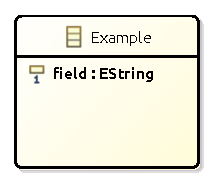
\includegraphics{images/05_library_of_transformations/02_type_level_transformations/06_data_fields/data_field.pdf}
        \caption{$Tm_{DataField}$ for a $\type{string}$ with $name = \type{field}$}
        \label{fig:library_of_transformations:type_level_transformations:data_fields:visualisation:ecore}
    \end{subfigure}
    \begin{subfigure}{0.45\textwidth}
        \centering
        \input{images/05_library_of_transformations/02_type_level_transformations/06_data_fields/data_field_as_edge_type.tikz}
        \caption{$TG_{DataField}$ for a $\type{string}$ with $name = \type{field}$}
        \label{fig:library_of_transformations:type_level_transformations:data_fields:visualisation:groove}
    \end{subfigure}
    \caption{Visualisation of the transformation of a field typed by a data type}
    \label{fig:library_of_transformations:type_level_transformations:data_fields:visualisation}
\end{figure}

All transformations discussed so far have focused on introducing different kind of types. In the following transformations, these types will be enriched with fields. In this transformation specifically, a field typed by a data type will be introduced.

\begin{defin}[Type model $Tm_{DataField}$]
\label{defin:library_of_transformations:type_level_transformations:data_fields:tmod_data_field}
Let $Tm_{DataField}$ be the type model containing a regular class with identifier $classtype$. Then $Tm_{DataField}$ defines a field named $name$ with type $fieldtype$, in which $fieldtype$ is either $\type{boolean}$, $\type{integer}$, $\type{real}$ or $\type{string}$. $Tm_{DataField}$ is defined as:
\begin{align*}
Class =\ &\{classtype\} \\
Enum =\ &\{\} \\
UserDataType =\ &\{\} \\
Field =\ &\{(classtype, name)\} \\
\mathrm{FieldSig} =\ &\begin{cases}
    (f, (fieldtype, 1..1)) &\mathrm{if}\ f \in Field_{Tm_{DataField}}
\end{cases} \\
EnumValue =\ &\{\} \\
Inh =\ &\{\} \\
Prop =\ &\{\} \\
Constant =\ &\{\} \\
\mathrm{ConstType} =\ &\{\}
\end{align*}
\isabellelref{tmod_data_field}{Ecore-GROOVE-Mapping-Library.DataField}
\end{defin}

\begin{thm}[Correctness of $Tm_{DataField}$]
\label{defin:library_of_transformations:type_level_transformations:data_fields:tmod_data_field_correct}
$Tm_{DataField}$ (\cref{defin:library_of_transformations:type_level_transformations:data_fields:tmod_data_field}) is a consistent type model in the sense of \cref{defin:formalisations:ecore_formalisation:type_models:type_model_consistency}.
\isabellelref{tmod_data_field_correct}{Ecore-GROOVE-Mapping-Library.DataField}
\end{thm}

A visual representation of $Tm_{DataField}$ with field name $\type{field}$ on class $.\type{Example}$ can be seen in \cref{fig:library_of_transformations:type_level_transformations:data_fields:visualisation:ecore}. In this example, the $\type{string}$ type is chosen for the fieldtype, but any data type would have worked. The correctness proof of $Tm_{DataField}$ is more involved, it is not included here for conciseness. It can be found within the validated Isabelle proofs.

In order to make composing transformation functions possible, $Tm_{DataField}$ should be compatible with the type model it is combined with.

\begin{thm}[Correctness of $\mathrm{combine}(Tm, Tm_{DataField})$]
\label{defin:library_of_transformations:type_level_transformations:data_fields:tmod_data_field_combine_correct}
Assume a type model $Tm$ that is consistent in the sense of \cref{defin:formalisations:ecore_formalisation:type_models:type_model_consistency}. Then $Tm$ is compatible with $Tm_{DataField}$ (in the sense of \cref{defin:transformation_framework:type_models_and_type_graphs:combining_type_models:compatibility}) if:
\begin{itemize}
    \item The class type on which the field is defined, $classtype$, is already an existing class in $Tm$;
    \item The field named $name$ is not already a field on $classtype$ in $Tm$.
\end{itemize}
\isabellelref{tmod_data_field_combine_correct}{Ecore-GROOVE-Mapping-Library.DataField}
\end{thm}

\begin{proof}
Use \cref{defin:transformation_framework:type_models_and_type_graphs:combining_type_models:tmod_combine_merge_correct}. It is possible to show that all assumptions hold. Now we have shown that $\mathrm{combine}(Tm, Tm_{DataField})$ is consistent in the sense of \cref{defin:formalisations:ecore_formalisation:type_models:type_model_consistency}.
\end{proof}

The definitions and theorems for defining a data field within Ecore are now complete. 

\subsubsection{Encoding as edge type}

The most obvious encoding for an field in GROOVE would be using an edge type. The field is transformed into an edge type between an existing node type and the corresponding field type. The encoding corresponding to $Tm_{DataField}$ can then be represented as $TG_{DataField}$, defined in the following definition:

\begin{defin}[Type graph $TG_{DataField}$]
\label{defin:library_of_transformations:type_level_transformations:data_fields:tg_data_field_as_edge_type}
Let $TG_{DataField}$ be the type graph containing a node type which encodes the class type $classtype$. Furthermore, define an edge type from $classtype$ named $name$. This edge type targets a node of $fieldtype$. $TG_{DataField}$ is defined as:
\begin{align*}
NT =\ &\{\mathrm{ns\_\!to\_\!list}(classtype), fieldtype\} \\
ET =\ &\{(\mathrm{ns\_\!to\_\!list}(classtype), \langle name \rangle, fieldtype)\} \\
\!\!\sqsubseteq\ =\ &\{( \mathrm{ns\_\!to\_\!list}(classtype), \mathrm{ns\_\!to\_\!list}(classtype) ), ( fieldtype, fieldtype )\} \\
abs =\ &\{\} \\
\mathrm{mult}(e) =\ &\begin{cases}
    (0..\mstar, 1..1) &\mathrm{if}\ e \in \{(\mathrm{ns\_\!to\_\!list}(classtype), \langle name \rangle, fieldtype)\}
\end{cases} \\
contains =\ &\{\}
\end{align*}
\isabellelref{tg_data_field_as_edge_type}{Ecore-GROOVE-Mapping-Library.DataField}
\end{defin}

\begin{thm}[Correctness of $TG_{DataField}$]
\label{defin:library_of_transformations:type_level_transformations:data_fields:tg_data_field_as_edge_type_correct}
$TG_{DataField}$ (\cref{defin:library_of_transformations:type_level_transformations:data_fields:tg_data_field_as_edge_type}) is a valid type graph in the sense of \cref{defin:formalisations:groove_formalisation:type_graphs:type_graph_validity}.
\isabellelref{tg_data_field_as_edge_type_correct}{Ecore-GROOVE-Mapping-Library.DataField}
\end{thm}

A visual representation of $TG_{DataField}$ with edge name $\type{field}$ on node type $\type{Example}$ can be seen in \cref{fig:library_of_transformations:type_level_transformations:data_fields:visualisation:groove}. Like the previous example, a $\type{string}$ has been chosen to be consequent, but any primitive type could have been used. The correctness proof of $TG_{DataField}$ is more involved, it is not included here for conciseness. It can be found within the validated Isabelle proofs.

In order to make composing transformation functions possible, $TG_{DataField}$ should be compatible with the type graph it is combined with.

\begin{thm}[Correctness of $\mathrm{combine}(TG, TG_{DataField})$]
\label{defin:library_of_transformations:type_level_transformations:data_fields:tg_data_field_as_edge_type_combine_correct}
Assume a type graph $TG$ that is valid in the sense of \cref{defin:formalisations:groove_formalisation:type_graphs:type_graph_validity}. Then $TG$ is compatible with $TG_{DataField}$ (in the sense of \cref{defin:transformation_framework:type_models_and_type_graphs:combining_type_graphs:compatibility}) if:
\begin{itemize}
    \item The node type of the encoded class type in $TG_{DataField}$ is already an node type in $TG$;
    \item The node type of the encoded class type in $TG_{DataField}$ does not already have an edge type with the same name as the field in $TG$.
\end{itemize}
\isabellelref{tg_data_field_as_edge_type_combine_correct}{Ecore-GROOVE-Mapping-Library.DataField}
\end{thm}

\begin{proof}
Use \cref{defin:transformation_framework:type_models_and_type_graphs:combining_type_graphs:tg_combine_merge_correct}. It is possible to show that all assumptions hold. Now we have shown that $\mathrm{combine}(TG, TG_{DataField})$ is valid in the sense of \cref{defin:formalisations:groove_formalisation:type_graphs:type_graph_validity}.
\end{proof}

The next definitions define the transformation function from $Tm_{DataField}$ to $TG_{DataField}$:

\begin{defin}[Transformation function $f_{DataField}$]
\label{defin:library_of_transformations:type_level_transformations:data_fields:tmod_data_field_to_tg_data_field_as_edge_type}
The transformation function $f_{DataField}(Tm)$ is defined as:
\begin{align*}
NT =\ &\{\mathrm{ns\_\!to\_\!list}(c) \mid c \in Class_{Tm}\} \cup \{fieldtype\}\\
ET =\ &\{(\mathrm{ns\_\!to\_\!list}(c), \langle f \rangle, fieldtype) \mid (c, n) \in Field_{Tm} \} \\
\!\!\sqsubseteq\ =\ &\{( \mathrm{ns\_\!to\_\!list}(c), \mathrm{ns\_\!to\_\!list}(c) ) \mid c \in Class_{Tm} \} \cup \{( fieldtype, fieldtype ) \} \\
abs =\ &\{\} \\
\mathrm{mult} =\ &\begin{cases}
    (0..\mstar, 1..1) &\mathrm{if}\ e \in \{(\mathrm{ns\_\!to\_\!list}(c), \langle f \rangle, fieldtype) \mid (c, n) \in Field_{Tm} \}
\end{cases} \\
contains =\ &\{\}
\end{align*}
\isabellelref{tmod_data_field_to_tg_data_field_as_edge_type}{Ecore-GROOVE-Mapping-Library.DataField}
\end{defin}

\begin{thm}[Correctness of $f_{DataField}$]
\label{defin:library_of_transformations:type_level_transformations:data_fields:tmod_data_field_to_tg_data_field_as_edge_type_func}
$f_{DataField}(Tm)$ (\cref{defin:library_of_transformations:type_level_transformations:data_fields:tmod_data_field_to_tg_data_field_as_edge_type}) is a valid transformation function in the sense of \cref{defin:transformation_framework:type_models_and_type_graphs:combining_transformation_functions:transformation_function_type_model_type_graph} transforming $Tm_{DataField}$ into $TG_{DataField}$.
\isabellelref{tmod_data_field_to_tg_data_field_as_edge_type_func}{Ecore-GROOVE-Mapping-Library.DataField}
\end{thm}

The proof of the correctness of $f_{DataField}$ will not be included here. Instead, it can be found in the validated Isabelle theories.

Finally, to complete the transformation, the transformation function that transforms $TG_{DataField}$ into $Tm_{DataField}$ is defined:

\begin{defin}[Transformation function $f'_{DataField}$]
\label{defin:library_of_transformations:type_level_transformations:data_fields:tg_data_field_as_edge_type_to_tmod_data_field}
The transformation function $f'_{DataField}(TG)$ is defined as:
\begin{align*}
Class =\ &\{\mathrm{list\_\!to\_\!ns}(n) \mid n \in NT_{TG} \cap Lab_t \} \\
Enum =\ &\{\} \\
UserDataType =\ &\{\} \\
Field =\ &\{(\mathrm{list\_\!to\_\!ns}(\mathrm{src}(e)), l) \mid e \in ET_{TG} \land \langle l \rangle = \mathrm{lab}(e) \} \\
\mathrm{FieldSig} =\ &\begin{cases}
    (f, (fieldtype, 1..1)) &\mathrm{if}\ f \in \{(\mathrm{list\_\!to\_\!ns}(\mathrm{src}(e)), l) \mid e \in ET_{TG} \land \langle l \rangle = \mathrm{lab}(e) \} 
\end{cases} \\
EnumValue =\ &\{\} \\
Inh =\ &\{\} \\
Prop =\ &\{\} \\
Constant =\ &\{\} \\
\mathrm{ConstType} =\ &\{\}
\end{align*}
\isabellelref{tg_data_field_as_edge_type_to_tmod_data_field}{Ecore-GROOVE-Mapping-Library.DataField}
\end{defin}

\begin{thm}[Correctness of $f'_{DataField}$]
\label{defin:library_of_transformations:type_level_transformations:data_fields:tg_data_field_as_edge_type_to_tmod_data_field_func}
$f'_{DataField}(TG)$ (\cref{defin:library_of_transformations:type_level_transformations:data_fields:tg_data_field_as_edge_type_to_tmod_data_field}) is a valid transformation function in the sense of \cref{defin:transformation_framework:type_models_and_type_graphs:combining_transformation_functions:transformation_function_type_graph_type_model} transforming $TG_{DataField}$ into $Tm_{DataField}$.
\isabellelref{tg_data_field_as_edge_type_to_tmod_data_field_func}{Ecore-GROOVE-Mapping-Library.DataField}
\end{thm}

Once more, the correctness proof is not included here but can be found in the validated Isabelle proofs of this thesis.
\subsection{Enumeration fields}
\label{subsec:library_of_transformations:type_level_transformations:enum_fields}

\begin{figure}
    \centering
    \begin{subfigure}{0.45\textwidth}
        \centering
        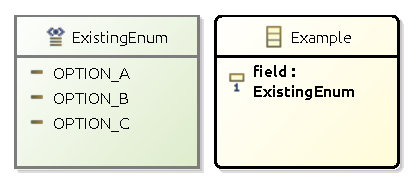
\includegraphics{images/05_library_of_transformations/02_type_level_transformations/07_enum_fields/enum_field.pdf}
        \caption{$Tm_{EnumField}$ for $.\type{ExistingEnum}$ \\with $name = \type{field}$}
        \label{fig:library_of_transformations:type_level_transformations:enum_fields:visualisation:ecore}
    \end{subfigure}
    \begin{subfigure}{0.45\textwidth}
        \centering
        \input{images/05_library_of_transformations/02_type_level_transformations/07_enum_fields/enum_as_flags_field_as_edge_type.tikz}
        \caption{$TG_{EnumFieldFlags}$ for $\type{ExistingEnum}$ \\with $name = \type{field}$}
        \label{fig:library_of_transformations:type_level_transformations:enum_fields:visualisation:groove_flags}
    \end{subfigure}
    \\
    \begin{subfigure}{0.95\textwidth}
        \centering
        \input{images/05_library_of_transformations/02_type_level_transformations/07_enum_fields/enum_as_node_types_field_as_edge_type.tikz}
        \caption{$TG_{EnumFieldNodes}$ for $\type{ExistingEnum}$ with $name = \type{field}$}
        \label{fig:library_of_transformations:type_level_transformations:enum_fields:visualisation:groove_nodes}
    \end{subfigure}
    \caption{Visualisation of the transformation of a field typed by an enumeration type}
    \label{fig:library_of_transformations:type_level_transformations:enum_fields:visualisation}
\end{figure}

In this section, the transformation for a field typed by an enumeration type will be discussed. Since an enumeration type can be encoded in multiple ways, multiple encodings will be introduced for fields as well. First, the Ecore type model will be introduced.

\begin{defin}[Type model $Tm_{EnumField}$]
\label{defin:library_of_transformations:type_level_transformations:enum_fields:tmod_enum_field}
Let $Tm_{EnumField}$ be the type model containing a regular class with identifier $classtype$. Furthermore, it defines an enumeration type with identifier $enumid$, and corresponding values as set $enumvalues$. Then $Tm_{EnumField}$ defines a field named $name$ with type $enumid$ on class $classtype$. $Tm_{EnumField}$ is defined as:
\begin{align*}
Class =\ &\{classtype\} \\
Enum =\ &\{enumid\} \\
UserDataType =\ &\{\} \\
Field =\ &\{(classtype, name)\} \\
\mathrm{FieldSig} =\ &\begin{cases}
    (f, (enumid, 1..1)) &\mathrm{if}\ f \in Field_{Tm_{EnumField}}
\end{cases} \\
EnumValue =\ &\{(enumid, v) \mid v \in enumvalues\} \\
Inh =\ &\{\} \\
Prop =\ &\{\} \\
Constant =\ &\{\} \\
\mathrm{ConstType} =\ &\{\}
\end{align*}
\isabellelref{tmod_enum_field}{Ecore-GROOVE-Mapping-Library.EnumField}
\end{defin}

\begin{thm}[Correctness of $Tm_{EnumField}$]
\label{defin:library_of_transformations:type_level_transformations:enum_fields:tmod_enum_field_correct}
$Tm_{EnumField}$ (\cref{defin:library_of_transformations:type_level_transformations:enum_fields:tmod_enum_field}) is a consistent type model in the sense of \cref{defin:formalisations:ecore_formalisation:type_models:type_model_consistency}.
\isabellelref{tmod_enum_field_correct}{Ecore-GROOVE-Mapping-Library.EnumField}
\end{thm}

A visual representation of $Tm_{EnumField}$ with field name $\type{field}$ on class $.\type{Example}$ can be seen in \cref{fig:library_of_transformations:type_level_transformations:enum_fields:visualisation:ecore}. In this example, the field is typed by the $.\type{ExistingEnum}$ enumeration type. The correctness proof of $Tm_{EnumField}$ is more involved, it is not included here for conciseness. It can be found within the validated Isabelle proofs.

In order to make composing transformation functions possible, $Tm_{EnumField}$ should be compatible with the type model it is combined with.

\begin{thm}[Correctness of $\mathrm{combine}(Tm, Tm_{EnumField})$]
\label{defin:library_of_transformations:type_level_transformations:enum_fields:tmod_enum_field_combine_correct}
Assume a type model $Tm$ that is consistent in the sense of \cref{defin:formalisations:ecore_formalisation:type_models:type_model_consistency}. Then $Tm$ is compatible with $Tm_{EnumField}$ (in the sense of \cref{defin:transformation_framework:type_models_and_type_graphs:combining_type_models:compatibility}) if:
\begin{itemize}
    \item The class type on which the field is defined, $classtype$, is already an existing class in $Tm$;
    \item The enumeration type by which the field is typed, $enumid$, is already an existing enumeration type in $Tm$;
    \item All the values for the enumeration type $enumid$ are already enumeration values for $enumid$ in $Tm$;
    \item The field named $name$ is not already a field on $classtype$ in $Tm$.
\end{itemize}
\isabellelref{tmod_enum_field_combine_correct}{Ecore-GROOVE-Mapping-Library.EnumField}
\end{thm}

\begin{proof}
Use \cref{defin:transformation_framework:type_models_and_type_graphs:combining_type_models:tmod_combine_merge_correct}. It is possible to show that all assumptions hold. Now we have shown that $\mathrm{combine}(Tm, Tm_{EnumField})$ is consistent in the sense of \cref{defin:formalisations:ecore_formalisation:type_models:type_model_consistency}.
\end{proof}

The definitions and theorems for defining a field typed by an enumeration type within Ecore are now complete. 

\subsubsection{Encoding as edge type to an node type encoded enumeration type}

As mentioned earlier, \cref{subsec:library_of_transformations:type_level_transformations:enumeration_types} defines multiple ways to encode an enumeration type. Each of these encodings needs a specialised field encoding. In principle, the encoding of the fields itself is the same, but since every transformation model needs to be valid on its own, the encodings need to be distinguished. 

The first encoding for an enumeration type uses node types to encode the different values. The encoding corresponding to $Tm_{EnumField}$, in the case that the field references an enumeration type encoded as node types, can then be represented as $TG_{EnumFieldNodes}$, defined in the following definition:

\begin{defin}[Type graph $TG_{EnumFieldNodes}$]
\label{defin:library_of_transformations:type_level_transformations:enum_fields:tg_enum_as_node_types_field_as_edge_type}
Let $TG_{EnumFieldNodes}$ be the type graph containing a node type which encodes the class type $classtype$.
Furthermore, $TG_{EnumFieldNodes}$ contains an encoded version of enumeration type $enumid$ with values from set $enumvalues$. This enumeration type is encoded using node types, as defined in $TG_{EnumNodes}$ (\cref{defin:library_of_transformations:type_level_transformations:enumeration_types:tg_enum_as_node_types}). Finally, $TG_{EnumFieldNodes}$ defines an edge type from the encoded $classtype$ named $name$ to the encoded enumeration type $enumid$. $TG_{EnumFieldNodes}$ is defined as:
\begin{align*}
NT =\ &\{\mathrm{ns\_\!to\_\!list}(classtype), \mathrm{ns\_\!to\_\!list}(enumid)\}\ \cup \\&\{ \mathrm{ns\_\!to\_\!list}(enumid) \append \langle v \rangle \mid v \in enumvalues \}\\
ET =\ &\{(\mathrm{ns\_\!to\_\!list}(classtype), \langle name \rangle, \mathrm{ns\_\!to\_\!list}(enumid))\} \\
\!\!\sqsubseteq\ =\ &\{(\mathrm{ns\_\!to\_\!list}(classtype), \mathrm{ns\_\!to\_\!list}(classtype)),\ \\& (\mathrm{ns\_\!to\_\!list}(enumid), \mathrm{ns\_\!to\_\!list}(enumid))\}\ \cup \\&
\{(\mathrm{ns\_\!to\_\!list}(enumid) \append \langle v \rangle, \mathrm{ns\_\!to\_\!list}(enumid) \append \langle v \rangle) \mid v \in enumvalues \}\ \cup \\&
\{(\mathrm{ns\_\!to\_\!list}(enumid) \append \langle v \rangle, \mathrm{ns\_\!to\_\!list}(enumid)) \mid v \in enumvalues \} \\
abs =\ &\{\mathrm{ns\_\!to\_\!list}(enumid)\} \\
\mathrm{mult}(e) =\ &\begin{cases}
    (0..\mstar, 1..1) &\mathrm{if}\ e \in \{(\mathrm{ns\_\!to\_\!list}(classtype), \langle name \rangle, \mathrm{ns\_\!to\_\!list}(enumid))\}
\end{cases} \\
contains =\ &\{\}
\end{align*}
\isabellelref{tg_enum_as_node_types_field_as_edge_type}{Ecore-GROOVE-Mapping-Library.EnumField}
\end{defin}

\begin{thm}[Correctness of $TG_{EnumFieldNodes}$]
\label{defin:library_of_transformations:type_level_transformations:enum_fields:tg_enum_as_node_types_field_as_edge_type_correct}
$TG_{EnumFieldNodes}$ (\cref{defin:library_of_transformations:type_level_transformations:enum_fields:tg_enum_as_node_types_field_as_edge_type}) is a valid type graph in the sense of \cref{defin:formalisations:groove_formalisation:type_graphs:type_graph_validity}.
\isabellelref{tg_enum_as_node_types_field_as_edge_type_correct}{Ecore-GROOVE-Mapping-Library.EnumField}
\end{thm}

A visual representation of $TG_{EnumFieldNodes}$ with edge name $\type{field}$ on node type $\type{Example}$ can be seen in \cref{fig:library_of_transformations:type_level_transformations:enum_fields:visualisation:groove_nodes}. The field references the encoded enumeration type $\type{ExistingEnum}$ via the abstract type, such that its nodes can reference any of the concrete values. The correctness proof of $TG_{EnumFieldNodes}$ is more involved, it is not included here for conciseness. It can be found within the validated Isabelle proofs.

In order to make composing transformation functions possible, $TG_{EnumFieldNodes}$ should be compatible with the type graph it is combined with.

\begin{thm}[Correctness of $\mathrm{combine}(TG, TG_{EnumFieldNodes})$]
\label{defin:library_of_transformations:type_level_transformations:enum_fields:tg_enum_as_node_types_field_as_edge_type_combine_correct}
Assume a type graph $TG$ that is valid in the sense of \cref{defin:formalisations:groove_formalisation:type_graphs:type_graph_validity}. Then $TG$ is compatible with $TG_{EnumFieldNodes}$ (in the sense of \cref{defin:transformation_framework:type_models_and_type_graphs:combining_type_graphs:compatibility}) if:
\begin{itemize}
    \item The node type of the encoded class type in $TG_{EnumFieldNodes}$ is already an node type in $TG$;
    \item All node types corresponding to the encoding of the enumeration type in $TG_{EnumFieldNodes}$ are already node types in $TG$;
    \item The node type of the encoded class type in $TG_{EnumFieldNodes}$ does not already have an edge type with the same name as the field in $TG$.
\end{itemize}
\isabellelref{tg_enum_as_node_types_field_as_edge_type_combine_correct}{Ecore-GROOVE-Mapping-Library.EnumField}
\end{thm}

\begin{proof}
Use \cref{defin:transformation_framework:type_models_and_type_graphs:combining_type_graphs:tg_combine_merge_correct}. It is possible to show that all assumptions hold. Now we have shown that $\mathrm{combine}(TG, TG_{EnumFieldNodes})$ is valid in the sense of \cref{defin:formalisations:groove_formalisation:type_graphs:type_graph_validity}.
\end{proof}

The next definitions define the transformation function from $Tm_{EnumField}$ to $TG_{EnumFieldNodes}$:

\begin{defin}[Transformation function $f_{EnumFieldNodes}$]
\label{defin:library_of_transformations:type_level_transformations:enum_fields:tmod_enum_field_to_tg_enum_as_node_types_field_as_edge_type}
The transformation function $f_{EnumFieldNodes}(Tm)$ is defined as:
\begin{align*}
NT =\ &\{\mathrm{ns\_\!to\_\!list}(t) \mid t \in Class_{Tm} \cup Enum_{Tm}\}\ \cup \\&\{ \mathrm{ns\_\!to\_\!list}(e) \append \langle v \rangle \mid (e, v) \in EnumValue_{Tm} \}\\
ET =\ &\{(\mathrm{ns\_\!to\_\!list}(c), \langle f \rangle, \mathrm{ns\_\!to\_\!list}(e)) \mid (c, f) \in Field_{Tm} \land e \in Enum_{Tm}\} \\
\!\!\sqsubseteq\ =\ &\{(\mathrm{ns\_\!to\_\!list}(x), \mathrm{ns\_\!to\_\!list}(x)) \mid x \in Class_{Tm} \cup Enum_{Tm} \}\ \cup \\&
\{(\mathrm{ns\_\!to\_\!list}(e) \append \langle v \rangle, \mathrm{ns\_\!to\_\!list}(e) \append \langle v \rangle) \mid (e, v) \in EnumValue_{Tm} \}\ \cup \\&
\{(\mathrm{ns\_\!to\_\!list}(e) \append \langle v \rangle, \mathrm{ns\_\!to\_\!list}(e)) \mid (e, v) \in EnumValue_{Tm} \} \\
abs =\ &\{\mathrm{ns\_\!to\_\!list}(t) \mid t \in Enum_{Tm}\}\ \\
\mathrm{mult}(e) =\ &\begin{cases}
    (0..\mstar, 1..1) &\mathrm{if}\ e \in \{(\mathrm{ns\_\!to\_\!list}(c), \langle f \rangle, \mathrm{ns\_\!to\_\!list}(e)) \mid (c, f) \in Field_{Tm} \land e \in Enum_{Tm}\}
\end{cases} \\
contains =\ &\{\}
\end{align*}
\isabellelref{tmod_enum_field_to_tg_enum_as_node_types_field_as_edge_type}{Ecore-GROOVE-Mapping-Library.EnumField}
\end{defin}

\begin{thm}[Correctness of $f_{EnumFieldNodes}$]
\label{defin:library_of_transformations:type_level_transformations:enum_fields:tmod_enum_field_to_tg_enum_as_node_types_field_as_edge_type_func}
$f_{EnumFieldNodes}(Tm)$ (\cref{defin:library_of_transformations:type_level_transformations:enum_fields:tmod_enum_field_to_tg_enum_as_node_types_field_as_edge_type}) is a valid transformation function in the sense of \cref{defin:transformation_framework:type_models_and_type_graphs:combining_transformation_functions:transformation_function_type_model_type_graph} transforming $Tm_{EnumField}$ into $TG_{EnumFieldNodes}$.
\isabellelref{tmod_enum_field_to_tg_enum_as_node_types_field_as_edge_type_func}{Ecore-GROOVE-Mapping-Library.EnumField}
\end{thm}

The proof of the correctness of $f_{EnumFieldNodes}$ will not be included here. Instead, it can be found in the validated Isabelle theories.

Finally, to complete the transformation, the transformation function that transforms $TG_{EnumFieldNodes}$ into $Tm_{EnumField}$ is defined:

\begin{defin}[Transformation function $f'_{EnumFieldNodes}$]
\label{defin:library_of_transformations:type_level_transformations:enum_fields:tg_enum_as_node_types_field_as_edge_type_to_tmod_enum_field}
The transformation function $f'_{EnumFieldNodes}(TG)$ is defined as:
\begin{align*}
Class =\ &\{\mathrm{list\_\!to\_\!ns}(n) \mid n \in NT_{TG} \land n = \mathrm{ns\_\!to\_\!list}(classtype) \} \\
Enum =\ &\{\mathrm{list\_\!to\_\!ns}(n) \mid n \in NT_{TG} \land n = \mathrm{ns\_\!to\_\!list}(enumid) \} \\
UserDataType =\ &\{\} \\
Field =\ &\{(\mathrm{list\_\!to\_\!ns}(\mathrm{src}(e)), l) \mid e \in ET_{TG} \land \langle l \rangle = \mathrm{lab}(e) \} \\
\mathrm{FieldSig} =\ &\begin{cases}
    (f, (fieldtype, 1..1)) &\mathrm{if}\ f \in \{(\mathrm{list\_\!to\_\!ns}(\mathrm{src}(e)), l) \mid e \in ET_{TG} \land \langle l \rangle = \mathrm{lab}(e) \}
\end{cases} \\
EnumValue =\ &\{(enumid, v) \mid v \in enumvalues\} \\
Inh =\ &\{\} \\
Prop =\ &\{\} \\
Constant =\ &\{\} \\
\mathrm{ConstType} =\ &\{\}
\end{align*}
\isabellelref{tg_enum_as_node_types_field_as_edge_type_to_tmod_enum_field}{Ecore-GROOVE-Mapping-Library.EnumField}
\end{defin}

\begin{thm}[Correctness of $f'_{EnumFieldNodes}$]
\label{defin:library_of_transformations:type_level_transformations:enum_fields:tg_enum_as_node_types_field_as_edge_type_to_tmod_enum_field_func}
$f'_{EnumFieldNodes}(TG)$ (\cref{defin:library_of_transformations:type_level_transformations:enum_fields:tg_enum_as_node_types_field_as_edge_type_to_tmod_enum_field}) is a valid transformation function in the sense of \cref{defin:transformation_framework:type_models_and_type_graphs:combining_transformation_functions:transformation_function_type_graph_type_model} transforming $TG_{EnumFieldNodes}$ into $Tm_{EnumField}$.
\isabellelref{tg_enum_as_node_types_field_as_edge_type_to_tmod_enum_field_func}{Ecore-GROOVE-Mapping-Library.EnumField}
\end{thm}

Once more, the correctness proof is not included here but can be found in the validated Isabelle proofs of this thesis.

\subsubsection{Encoding as edge type to an flag encoded enumeration type}

The second encoding for an enumeration type uses flags to encode the different values. The encoding corresponding to $Tm_{EnumField}$, in the case that the field references an enumeration type encoded as flags, can then be represented as $TG_{EnumFieldFlags}$, defined in the following definition:

\begin{defin}[Type graph $TG_{EnumFieldFlags}$]
\label{defin:library_of_transformations:type_level_transformations:enum_fields:tg_enum_as_flags_field_as_edge_type}
Let $TG_{EnumFieldFlags}$ be the type graph containing a node type which encodes the class type $classtype$.
Furthermore, $TG_{EnumFieldFlags}$ contains an encoded version of enumeration type $enumid$ with values from set $enumvalues$. This enumeration type is encoded using flags, as defined in $TG_{EnumFlags}$ (\cref{defin:library_of_transformations:type_level_transformations:enumeration_types:tg_enum_as_flags}). Finally, $TG_{EnumFieldFlags}$ defines an edge type from the encoded $classtype$ named $name$ to the encoded enumeration type $enumid$. $TG_{EnumFieldFlags}$ is defined as:
\begin{align*}
NT =\ &\{\mathrm{ns\_\!to\_\!list}(classtype), \mathrm{ns\_\!to\_\!list}(enumid)\}\\
ET =\ &\{(\mathrm{ns\_\!to\_\!list}(classtype), \langle name \rangle, \mathrm{ns\_\!to\_\!list}(enumid))\}\\
\!\!\sqsubseteq\ =\ &\{(\mathrm{ns\_\!to\_\!list}(classtype), \mathrm{ns\_\!to\_\!list}(classtype)),\ \\& (\mathrm{ns\_\!to\_\!list}(enumid), \mathrm{ns\_\!to\_\!list}(enumid))\}\\
abs =\ &\{\} \\
\mathrm{mult}(e) =\ &\begin{cases}
    (0..\mstar, 1..1) &\mathrm{if}\ e \in \{(\mathrm{ns\_\!to\_\!list}(classtype), \langle name \rangle, \mathrm{ns\_\!to\_\!list}(enumid))\}
\end{cases} \\
contains =\ &\{\}
\end{align*}
\isabellelref{tg_enum_as_flags_field_as_edge_type}{Ecore-GROOVE-Mapping-Library.EnumField}
\end{defin}

\begin{thm}[Correctness of $TG_{EnumFieldFlags}$]
\label{defin:library_of_transformations:type_level_transformations:enum_fields:tg_enum_as_flags_field_as_edge_type_correct}
$TG_{EnumFieldFlags}$ (\cref{defin:library_of_transformations:type_level_transformations:enum_fields:tg_enum_as_flags_field_as_edge_type}) is a valid type graph in the sense of \cref{defin:formalisations:groove_formalisation:type_graphs:type_graph_validity}.
\isabellelref{tg_enum_as_flags_field_as_edge_type_correct}{Ecore-GROOVE-Mapping-Library.EnumField}
\end{thm}

A visual representation of $TG_{EnumFieldFlags}$ with edge name $\type{field}$ on node type $\type{Example}$ can be seen in \cref{fig:library_of_transformations:type_level_transformations:enum_fields:visualisation:groove_flags}. The field references the encoded enumeration type $\type{ExistingEnum}$ via the corresponding node type. The correctness proof of $TG_{EnumFieldFlags}$ is more involved, it is not included here for conciseness. It can be found within the validated Isabelle proofs.

In order to make composing transformation functions possible, $TG_{EnumFieldFlags}$ should be compatible with the type graph it is combined with.

\begin{thm}[Correctness of $\mathrm{combine}(TG, TG_{EnumFieldFlags})$]
\label{defin:library_of_transformations:type_level_transformations:enum_fields:tg_enum_as_flags_field_as_edge_type_combine_correct}
Assume a type graph $TG$ that is valid in the sense of \cref{defin:formalisations:groove_formalisation:type_graphs:type_graph_validity}. Then $TG$ is compatible with $TG_{EnumFieldFlags}$ (in the sense of \cref{defin:transformation_framework:type_models_and_type_graphs:combining_type_graphs:compatibility}) if:
\begin{itemize}
    \item The node type of the encoded class type in $TG_{EnumFieldFlags}$ is already an node type in $TG$;
    \item All node types corresponding to the encoding of the enumeration type in $TG_{EnumFieldFlags}$ are already node types in $TG$;
    \item The node type of the encoded class type in $TG_{EnumFieldFlags}$ does not already have an edge type with the same name as the field in $TG$.
\end{itemize}
\isabellelref{tg_enum_as_flags_field_as_edge_type_combine_correct}{Ecore-GROOVE-Mapping-Library.EnumField}
\end{thm}

\begin{proof}
Use \cref{defin:transformation_framework:type_models_and_type_graphs:combining_type_graphs:tg_combine_merge_correct}. It is possible to show that all assumptions hold. Now we have shown that $\mathrm{combine}(TG, TG_{EnumFieldFlags})$ is valid in the sense of \cref{defin:formalisations:groove_formalisation:type_graphs:type_graph_validity}.
\end{proof}

The next definitions define the transformation function from $Tm_{EnumField}$ to $TG_{EnumFieldFlags}$:

\begin{defin}[Transformation function $f_{EnumFieldFlags}$]
\label{defin:library_of_transformations:type_level_transformations:enum_fields:tmod_enum_field_to_tg_enum_as_flags_field_as_edge_type}
The transformation function $f_{EnumFieldFlags}(Tm)$ is defined as:
\begin{align*}
NT =\ &\{\mathrm{ns\_\!to\_\!list}(t) \mid t \in Class_{Tm} \cup Enum_{Tm}\}\\
ET =\ &\{(\mathrm{ns\_\!to\_\!list}(c), \langle f \rangle, \mathrm{ns\_\!to\_\!list}(e)) \mid (c, f) \in Field_{Tm} \land e \in Enum_{Tm}\} \\
\!\!\sqsubseteq\ =\ &\{(\mathrm{ns\_\!to\_\!list}(x), \mathrm{ns\_\!to\_\!list}(x)) \mid x \in Class_{Tm} \cup Enum_{Tm} \}\\
abs =\ &\{\}\ \\
\mathrm{mult}(e) =\ &\begin{cases}
    (0..\mstar, 1..1) &\mathrm{if}\ e \in \{(\mathrm{ns\_\!to\_\!list}(c), \langle f \rangle, \mathrm{ns\_\!to\_\!list}(e)) \mid (c, f) \in Field_{Tm} \land e \in Enum_{Tm}\}
\end{cases} \\
contains =\ &\{\}
\end{align*}
\isabellelref{tmod_enum_field_to_tg_enum_as_flags_field_as_edge_type}{Ecore-GROOVE-Mapping-Library.EnumField}
\end{defin}

\begin{thm}[Correctness of $f_{EnumFieldFlags}$]
\label{defin:library_of_transformations:type_level_transformations:enum_fields:tmod_enum_field_to_tg_enum_as_flags_field_as_edge_type_func}
$f_{EnumFieldFlags}(Tm)$ (\cref{defin:library_of_transformations:type_level_transformations:enum_fields:tmod_enum_field_to_tg_enum_as_flags_field_as_edge_type}) is a valid transformation function in the sense of \cref{defin:transformation_framework:type_models_and_type_graphs:combining_transformation_functions:transformation_function_type_model_type_graph} transforming $Tm_{EnumField}$ into $TG_{EnumFieldFlags}$.
\isabellelref{tmod_enum_field_to_tg_enum_as_flags_field_as_edge_type_func}{Ecore-GROOVE-Mapping-Library.EnumField}
\end{thm}

The proof of the correctness of $f_{EnumFieldFlags}$ will not be included here. Instead, it can be found in the validated Isabelle theories.

Finally, to complete the transformation, the transformation function that transforms $TG_{EnumFieldFlags}$ into $Tm_{EnumField}$ is defined:

\begin{defin}[Transformation function $f'_{EnumFieldFlags}$]
\label{defin:library_of_transformations:type_level_transformations:enum_fields:tg_enum_as_flags_field_as_edge_type_to_tmod_enum_field}
The transformation function $f'_{EnumFieldFlags}(TG)$ is defined as:
\begin{align*}
Class =\ &\{\mathrm{list\_\!to\_\!ns}(n) \mid n \in NT_{TG} \land n = \mathrm{ns\_\!to\_\!list}(classtype) \} \\
Enum =\ &\{\mathrm{list\_\!to\_\!ns}(n) \mid n \in NT_{TG} \land n = \mathrm{ns\_\!to\_\!list}(enumid) \} \\
UserDataType =\ &\{\} \\
Field =\ &\{(\mathrm{list\_\!to\_\!ns}(\mathrm{src}(e)), l) \mid e \in ET_{TG} \land \langle l \rangle = \mathrm{lab}(e) \} \\
\mathrm{FieldSig} =\ &\begin{cases}
    (f, (fieldtype, 1..1)) &\mathrm{if}\ f \in \{(\mathrm{list\_\!to\_\!ns}(\mathrm{src}(e)), l) \mid e \in ET_{TG} \land \langle l \rangle = \mathrm{lab}(e) \}
\end{cases} \\
EnumValue =\ &\{(enumid, v) \mid v \in enumvalues\} \\
Inh =\ &\{\} \\
Prop =\ &\{\} \\
Constant =\ &\{\} \\
\mathrm{ConstType} =\ &\{\}
\end{align*}
\isabellelref{tg_enum_as_flags_field_as_edge_type_to_tmod_enum_field}{Ecore-GROOVE-Mapping-Library.EnumField}
\end{defin}

\begin{thm}[Correctness of $f'_{EnumFieldFlags}$]
\label{defin:library_of_transformations:type_level_transformations:enum_fields:tg_enum_as_flags_field_as_edge_type_to_tmod_enum_field_func}
$f'_{EnumFieldFlags}(TG)$ (\cref{defin:library_of_transformations:type_level_transformations:enum_fields:tg_enum_as_flags_field_as_edge_type_to_tmod_enum_field}) is a valid transformation function in the sense of \cref{defin:transformation_framework:type_models_and_type_graphs:combining_transformation_functions:transformation_function_type_graph_type_model} transforming $TG_{EnumFieldFlags}$ into $Tm_{EnumField}$.
\isabellelref{tg_enum_as_flags_field_as_edge_type_to_tmod_enum_field_func}{Ecore-GROOVE-Mapping-Library.EnumField}
\end{thm}

Once more, the correctness proof is not included here but can be found in the validated Isabelle proofs of this thesis.
\subsection{Nullable class fields}
\label{subsec:library_of_transformations:type_level_transformations:nullable_class_fields}

\begin{figure}
    \centering
    \begin{subfigure}{0.95\textwidth}
        \centering
        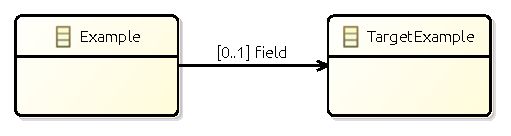
\includegraphics{images/05_library_of_transformations/02_type_level_transformations/08_nullable_class_fields/nullable_class_field.pdf}
        \caption{$Tm_{NullableClassField}$ to a class type $.\type{TargetExample}$ with $name = \type{field}$}
        \label{fig:library_of_transformations:type_level_transformations:nullable_class_fields:visualisation:ecore}
    \end{subfigure}
    \\
    \begin{subfigure}{0.95\textwidth}
        \centering
        \input{images/05_library_of_transformations/02_type_level_transformations/08_nullable_class_fields/nullable_class_field_as_edge_type.tikz}
        \caption{$TG_{NullableClassField}$ to a class type $\type{TargetExample}$ with $name = \type{field}$}
        \label{fig:library_of_transformations:type_level_transformations:nullable_class_fields:visualisation:groove}
    \end{subfigure}
    \caption{Visualisation of the transformation of a field typed by an optional class type}
    \label{fig:library_of_transformations:type_level_transformations:nullable_class_fields:visualisation}
\end{figure}

The previous sections have shown transformations of fields to attribute types. It has not shown any relations between objects yet. This transformation defines the transformation of a nullable class field.

\begin{defin}[Type model $Tm_{NullableClassField}$]
\label{defin:library_of_transformations:type_level_transformations:nullable_class_fields:tmod_nullable_class_field}
Let $Tm_{NullableClassField}$ be the type model containing a regular class with identifier $classtype$. Then $Tm_{NullableClassField}$ defines a field named $name$ with type $fieldtype$, in which $fieldtype$ is the identifier of another class type in $Tm_{NullableClassField}$. $Tm_{NullableClassField}$ is defined as:
\begin{align*}
Class =\ &\{classtype, fieldtype\} \\
Enum =\ &\{\} \\
UserDataType =\ &\{\} \\
Field =\ &\{(classtype, name)\} \\
\mathrm{FieldSig} =\ &\begin{cases}
    (f, (?fieldtype, 0..1)) &\mathrm{if}\ f \in Field_{Tm_{NullableClassField}}
\end{cases} \\
EnumValue =\ &\{\} \\
Inh =\ &\{\} \\
Prop =\ &\{\} \\
Constant =\ &\{\} \\
\mathrm{ConstType} =\ &\{\}
\end{align*}
\isabellelref{tmod_nullable_class_field}{Ecore-GROOVE-Mapping-Library.NullableClassField}
\end{defin}

\begin{thm}[Correctness of $Tm_{NullableClassField}$]
\label{defin:library_of_transformations:type_level_transformations:nullable_class_fields:tmod_nullable_class_field_correct}
$Tm_{NullableClassField}$ (\cref{defin:library_of_transformations:type_level_transformations:nullable_class_fields:tmod_nullable_class_field}) is a consistent type model in the sense of \cref{defin:formalisations:ecore_formalisation:type_models:type_model_consistency}.
\isabellelref{tmod_nullable_class_field_correct}{Ecore-GROOVE-Mapping-Library.NullableClassField}
\end{thm}

A visual representation of $Tm_{NullableClassField}$ with field name $\type{field}$ on class $.\type{Example}$ can be seen in \cref{fig:library_of_transformations:type_level_transformations:nullable_class_fields:visualisation:ecore}. In this example, $\type{field}$ references a class of $.\type{TargetExample}$. Please note that the lower bound of the multiplicity is 0 as the class is considered nullable. That means that setting a value for $\type{field}$ on class $.\type{Example}$ is optional. The correctness proof of $Tm_{NullableClassField}$ is more involved, it is not included here for conciseness. It can be found within the validated Isabelle proofs.

In order to make composing transformation functions possible, $Tm_{NullableClassField}$ should be compatible with the type model it is combined with.

\begin{thm}[Correctness of $\mathrm{combine}(Tm, Tm_{NullableClassField})$]
\label{defin:library_of_transformations:type_level_transformations:nullable_class_fields:tmod_nullable_class_field_combine_correct}
Assume a type model $Tm$ that is consistent in the sense of \cref{defin:formalisations:ecore_formalisation:type_models:type_model_consistency}. Then $Tm$ is compatible with $Tm_{NullableClassField}$ (in the sense of \cref{defin:transformation_framework:type_models_and_type_graphs:combining_type_models:compatibility}) if:
\begin{itemize}
    \item The class type on which the field is defined, $classtype$, is already an existing class in $Tm$;
    \item The class type which the field targets, $fieldtype$, is already an existing class in $Tm$;
    \item The field named $name$ is not already a field on $classtype$ in $Tm$.
\end{itemize}
\isabellelref{tmod_nullable_class_field_combine_correct}{Ecore-GROOVE-Mapping-Library.NullableClassField}
\end{thm}

\begin{proof}
Use \cref{defin:transformation_framework:type_models_and_type_graphs:combining_type_models:tmod_combine_merge_correct}. It is possible to show that all assumptions hold. Now we have shown that $\mathrm{combine}(Tm, Tm_{NullableClassField})$ is consistent in the sense of \cref{defin:formalisations:ecore_formalisation:type_models:type_model_consistency}.
\end{proof}

The definitions and theorems for defining a data field within Ecore are now complete. 

\subsubsection{Encoding as edge type}

Like any field definition so far, an edge type will be used within GROOVE to encode the field. The field is transformed into an edge type from the encoded class type to the encoded target type. The encoding corresponding to $Tm_{NullableClassField}$ can then be represented as $TG_{NullableClassField}$, defined in the following definition:

\begin{defin}[Type graph $TG_{NullableClassField}$]
\label{defin:library_of_transformations:type_level_transformations:nullable_class_fields:tg_nullable_class_field_as_edge_type}
Let $TG_{NullableClassField}$ be the type graph containing a node type which encodes the class type $classtype$. Furthermore, define an edge type from $classtype$ named $name$. This edge type targets a node of $fieldtype$. $TG_{NullableClassField}$ is defined as:
\begin{align*}
NT =\ &\{\mathrm{ns\_\!to\_\!list}(classtype), \mathrm{ns\_\!to\_\!list}(fieldtype)\} \\
ET =\ &\{(\mathrm{ns\_\!to\_\!list}(classtype), \langle name \rangle, \mathrm{ns\_\!to\_\!list}(fieldtype))\} \\
\!\!\sqsubseteq\ =\ &\{( \mathrm{ns\_\!to\_\!list}(classtype), \mathrm{ns\_\!to\_\!list}(classtype) ),\\&( \mathrm{ns\_\!to\_\!list}(fieldtype), \mathrm{ns\_\!to\_\!list}(fieldtype) )\} \\
abs =\ &\{\} \\
\mathrm{mult}(e) =\ &\begin{cases}
    (0..\mstar, 0..1) &\mathrm{if}\ e \in \{(\mathrm{ns\_\!to\_\!list}(classtype), \langle name \rangle, \mathrm{ns\_\!to\_\!list}(fieldtype))\}
\end{cases} \\
contains =\ &\{\}
\end{align*}
\isabellelref{tg_nullable_class_field_as_edge_type}{Ecore-GROOVE-Mapping-Library.NullableClassField}
\end{defin}

\begin{thm}[Correctness of $TG_{NullableClassField}$]
\label{defin:library_of_transformations:type_level_transformations:nullable_class_fields:tg_nullable_class_field_as_edge_type_correct}
$TG_{NullableClassField}$ (\cref{defin:library_of_transformations:type_level_transformations:nullable_class_fields:tg_nullable_class_field_as_edge_type}) is a valid type graph in the sense of \cref{defin:formalisations:groove_formalisation:type_graphs:type_graph_validity}.
\isabellelref{tg_nullable_class_field_as_edge_type_correct}{Ecore-GROOVE-Mapping-Library.NullableClassField}
\end{thm}

A visual representation of $TG_{NullableClassField}$ with edge name $\type{field}$ on node type $\type{Example}$ can be seen in \cref{fig:library_of_transformations:type_level_transformations:nullable_class_fields:visualisation:groove}. Like the previous example, $\type{field}$ references the $.\type{TargetExample}$ class, but in this case the encoded node type of $\type{TargetExample}$. The correctness proof of $TG_{NullableClassField}$ is more involved, it is not included here for conciseness. It can be found within the validated Isabelle proofs.

In order to make composing transformation functions possible, $TG_{NullableClassField}$ should be compatible with the type graph it is combined with.

\begin{thm}[Correctness of $\mathrm{combine}(TG, TG_{NullableClassField})$]
\label{defin:library_of_transformations:type_level_transformations:nullable_class_fields:tg_nullable_class_field_as_edge_type_combine_correct}
Assume a type graph $TG$ that is valid in the sense of \cref{defin:formalisations:groove_formalisation:type_graphs:type_graph_validity}. Then $TG$ is compatible with $TG_{NullableClassField}$ (in the sense of \cref{defin:transformation_framework:type_models_and_type_graphs:combining_type_graphs:compatibility}) if:
\begin{itemize}
    \item The node types of the encoded class types in $TG_{NullableClassField}$ are already node types in $TG$;
    \item The node type of the encoded class type in $TG_{NullableClassField}$ does not already have an edge type with the same name as the field in $TG$.
\end{itemize}
\isabellelref{tg_nullable_class_field_as_edge_type_combine_correct}{Ecore-GROOVE-Mapping-Library.NullableClassField}
\end{thm}

\begin{proof}
Use \cref{defin:transformation_framework:type_models_and_type_graphs:combining_type_graphs:tg_combine_merge_correct}. It is possible to show that all assumptions hold. Now we have shown that $\mathrm{combine}(TG, TG_{NullableClassField})$ is valid in the sense of \cref{defin:formalisations:groove_formalisation:type_graphs:type_graph_validity}.
\end{proof}

The next definitions define the transformation function from $Tm_{NullableClassField}$ to $TG_{NullableClassField}$:

\begin{defin}[Transformation function $f_{NullableClassField}$]
\label{defin:library_of_transformations:type_level_transformations:nullable_class_fields:tmod_nullable_class_field_to_tg_nullable_class_field_as_edge_type}
The transformation function $f_{NullableClassField}(Tm)$ is defined as:
\begin{align*}
NT =\ &\{\mathrm{ns\_\!to\_\!list}(c) \mid c \in Class_{Tm}\}\\
ET =\ &\{(\mathrm{ns\_\!to\_\!list}(c), \langle f \rangle, \mathrm{ns\_\!to\_\!list}(fieldtype)) \mid (c, n) \in Field_{Tm} \} \\
\!\!\sqsubseteq\ =\ &\{( \mathrm{ns\_\!to\_\!list}(c), \mathrm{ns\_\!to\_\!list}(c) ) \mid c \in Class_{Tm} \} \\
abs =\ &\{\} \\
\mathrm{mult} =\ &\begin{cases}
    (0..\mstar, 0..1) &\mathrm{if}\ e \in \{(\mathrm{ns\_\!to\_\!list}(c), \langle f \rangle, \mathrm{ns\_\!to\_\!list}(fieldtype)) \mid (c, n) \in Field_{Tm} \}
\end{cases} \\
contains =\ &\{\}
\end{align*}
\isabellelref{tmod_nullable_class_field_to_tg_nullable_class_field_as_edge_type}{Ecore-GROOVE-Mapping-Library.NullableClassField}
\end{defin}

\begin{thm}[Correctness of $f_{NullableClassField}$]
\label{defin:library_of_transformations:type_level_transformations:nullable_class_fields:tmod_nullable_class_field_to_tg_nullable_class_field_as_edge_type_func}
$f_{NullableClassField}(Tm)$ (\cref{defin:library_of_transformations:type_level_transformations:nullable_class_fields:tmod_nullable_class_field_to_tg_nullable_class_field_as_edge_type}) is a valid transformation function in the sense of \cref{defin:transformation_framework:type_models_and_type_graphs:combining_transformation_functions:transformation_function_type_model_type_graph} transforming $Tm_{NullableClassField}$ into $TG_{NullableClassField}$.
\isabellelref{tmod_nullable_class_field_to_tg_nullable_class_field_as_edge_type_func}{Ecore-GROOVE-Mapping-Library.NullableClassField}
\end{thm}

The proof of the correctness of $f_{NullableClassField}$ will not be included here. Instead, it can be found in the validated Isabelle theories.

Finally, to complete the transformation, the transformation function that transforms $TG_{NullableClassField}$ into $Tm_{NullableClassField}$ is defined:

\begin{defin}[Transformation function $f'_{NullableClassField}$]
\label{defin:library_of_transformations:type_level_transformations:nullable_class_fields:tg_nullable_class_field_as_edge_type_to_tmod_nullable_class_field}
The transformation function $f'_{NullableClassField}(TG)$ is defined as:
\begin{align*}
Class =\ &\{\mathrm{list\_\!to\_\!ns}(n) \mid n \in NT_{TG} \} \\
Enum =\ &\{\} \\
UserDataType =\ &\{\} \\
Field =\ &\{(\mathrm{list\_\!to\_\!ns}(\mathrm{src}(e)), l) \mid e \in ET_{TG} \land \langle l \rangle = \mathrm{lab}(e) \} \\
\mathrm{FieldSig} =\ &\begin{cases}
    (f, (?fieldtype, 0..1)) &\mathrm{if}\ f \in \{(\mathrm{list\_\!to\_\!ns}(\mathrm{src}(e)), l) \mid e \in ET_{TG} \land \langle l \rangle = \mathrm{lab}(e) \} 
\end{cases} \\
EnumValue =\ &\{\} \\
Inh =\ &\{\} \\
Prop =\ &\{\} \\
Constant =\ &\{\} \\
\mathrm{ConstType} =\ &\{\}
\end{align*}
\isabellelref{tg_nullable_class_field_as_edge_type_to_tmod_nullable_class_field}{Ecore-GROOVE-Mapping-Library.NullableClassField}
\end{defin}

\begin{thm}[Correctness of $f'_{NullableClassField}$]
\label{defin:library_of_transformations:type_level_transformations:nullable_class_fields:tg_nullable_class_field_as_edge_type_to_tmod_nullable_class_field_func}
$f'_{NullableClassField}(TG)$ (\cref{defin:library_of_transformations:type_level_transformations:nullable_class_fields:tg_nullable_class_field_as_edge_type_to_tmod_nullable_class_field}) is a valid transformation function in the sense of \cref{defin:transformation_framework:type_models_and_type_graphs:combining_transformation_functions:transformation_function_type_graph_type_model} transforming $TG_{NullableClassField}$ into $Tm_{NullableClassField}$.
\isabellelref{tg_nullable_class_field_as_edge_type_to_tmod_nullable_class_field_func}{Ecore-GROOVE-Mapping-Library.NullableClassField}
\end{thm}

Once more, the correctness proof is not included here but can be found in the validated Isabelle proofs of this thesis.
%\writingtask{Write about the proper class sequence field transformation}
\subsection{Contained class set fields}
\label{subsec:library_of_transformations:type_level_transformations:contained_class_set_fields}

\begin{figure}
    \centering
    \begin{subfigure}{0.95\textwidth}
        \centering
        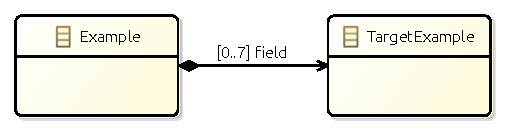
\includegraphics{images/05_library_of_transformations/02_type_level_transformations/10_contained_class_set_fields/contained_class_set_field.pdf}
        \caption{$Tm_{ContainedClassSetField}$ to a class type $.\type{TargetExample}$ with $name = \type{field}$}
        \label{fig:library_of_transformations:type_level_transformations:contained_class_set_fields:visualisation:ecore}
    \end{subfigure}
    \\
    \begin{subfigure}{0.95\textwidth}
        \centering
        \input{images/05_library_of_transformations/02_type_level_transformations/10_contained_class_set_fields/contained_class_set_as_edge_type.tikz}
        \caption{$TG_{ContainedClassSetField}$ to a class type $\type{TargetExample}$ with $name = \type{field}$}
        \label{fig:library_of_transformations:type_level_transformations:contained_class_set_fields:visualisation:groove}
    \end{subfigure}
    \caption{Visualisation of the transformation of a containment field typed by a set of a proper class type}
    \label{fig:library_of_transformations:type_level_transformations:contained_class_set_fields:visualisation}
\end{figure}

In this section, the transformation of a containment field typed by a set of a proper class type is shown. This transformation defines a field which has a value a set of objects of a specified class type, that is not nullable. Furthermore, the objects referenced by the field are contained by the source class. First, the Ecore type model is defined.

\begin{defin}[Type model $Tm_{ContainedClassSetField}$]
\label{defin:library_of_transformations:type_level_transformations:contained_class_set_fields:tmod_contained_class_set_field}
Let $Tm_{ContainedClassSetField}$ be the type model containing a regular class with identifier $classtype$. Then $Tm_{ContainedClassSetField}$ defines a field named $name$ with type $containedtype$, in which $containedtype$ is the identifier of another class type in $Tm_{ContainedClassSetField}$. Furthermore, define $mul$ to be a valid multiplicity for the field $name$. $Tm_{ContainedClassSetField}$ is defined as:
\begin{align*}
Class =\ &\{classtype, containedtype\} \\
Enum =\ &\{\} \\
UserDataType =\ &\{\} \\
Field =\ &\{(classtype, name)\} \\
\mathrm{FieldSig} =\ &\begin{cases}
    (f, ((\type{setof}, !containedtype), mul)) &\mathrm{if}\ f \in Field_{Tm_{ContainedClassSetField}}
\end{cases} \\
EnumValue =\ &\{\} \\
Inh =\ &\{\} \\
Prop =\ &\{(\type{containment}, (classtype, name))\} \\
Constant =\ &\{\} \\
\mathrm{ConstType} =\ &\{\}
\end{align*}
\isabellelref{tmod_contained_class_set_field}{Ecore-GROOVE-Mapping-Library.ContainedClassSetField}
\end{defin}

\begin{thm}[Correctness of $Tm_{ContainedClassSetField}$]
\label{defin:library_of_transformations:type_level_transformations:contained_class_set_fields:tmod_contained_class_set_field_correct}
$Tm_{ContainedClassSetField}$ (\cref{defin:library_of_transformations:type_level_transformations:contained_class_set_fields:tmod_contained_class_set_field}) is a consistent type model in the sense of \cref{defin:formalisations:ecore_formalisation:type_models:type_model_consistency}.
\isabellelref{tmod_contained_class_set_field_correct}{Ecore-GROOVE-Mapping-Library.ContainedClassSetField}
\end{thm}

A visual representation of $Tm_{ContainedClassSetField}$ with field name $\type{field}$ on class $.\type{Example}$ can be seen in \cref{fig:library_of_transformations:type_level_transformations:contained_class_set_fields:visualisation:ecore}. In this example, $\type{field}$ references a class of $.\type{TargetExample}$. Please note that the multiplicity $0..7$ has been chosen here as an example, any valid multiplicity could have been used. Also notice that the field is in fact a containment relation. The correctness proof of $Tm_{ContainedClassSetField}$ is more involved, it is not included here for conciseness. It can be found within the validated Isabelle proofs.

In order to make composing transformation functions possible, $Tm_{ContainedClassSetField}$ should be compatible with the type model it is combined with.

\begin{thm}[Correctness of $\mathrm{combine}(Tm, Tm_{ContainedClassSetField})$]
\label{defin:library_of_transformations:type_level_transformations:contained_class_set_fields:tmod_contained_class_set_field_combine_correct}
Assume a type model $Tm$ that is consistent in the sense of \cref{defin:formalisations:ecore_formalisation:type_models:type_model_consistency}. Then $Tm$ is compatible with $Tm_{ContainedClassSetField}$ (in the sense of \cref{defin:transformation_framework:type_models_and_type_graphs:combining_type_models:compatibility}) if:
\begin{itemize}
    \item The class type on which the field is defined, $classtype$, is already an existing class in $Tm$;
    \item The class type which the field targets, $containedtype$, is already an existing class in $Tm$;
    \item The field named $name$ is not already a field on $classtype$ in $Tm$;
    \item The multiplicity $mul$ is valid.
\end{itemize}
\isabellelref{tmod_contained_class_set_field_combine_correct}{Ecore-GROOVE-Mapping-Library.ContainedClassSetField}
\end{thm}

\begin{proof}
Use \cref{defin:transformation_framework:type_models_and_type_graphs:combining_type_models:tmod_combine_merge_correct}. It is possible to show that all assumptions hold. Now we have shown that $\mathrm{combine}(Tm, Tm_{ContainedClassSetField})$ is consistent in the sense of \cref{defin:formalisations:ecore_formalisation:type_models:type_model_consistency}.
\end{proof}

The definitions and theorems for defining a data field within Ecore are now complete. 

\subsubsection{Encoding as edge type}

Like the previous encodings of fields, an edge type in GROOVE will be used as encoding for the field. The field is transformed into an edge type from the encoded class type to the encoded target type. Furthermore, the edge type will be a containment edge, to support the fact that the target nodes are contained by the source nodes. The encoding corresponding to $Tm_{ContainedClassSetField}$ can then be represented as $TG_{ContainedClassSetField}$, defined in the following definition:

\begin{defin}[Type graph $TG_{ContainedClassSetField}$]
\label{defin:library_of_transformations:type_level_transformations:contained_class_set_fields:tg_contained_class_set_field_as_edge_type}
Let $TG_{ContainedClassSetField}$ be the type graph containing a node type which encodes the class type $classtype$. Furthermore, define an edge type from $classtype$ named $name$. This edge type targets a node of $containedtype$. Finally, define multiplicity $mul$ to be  $TG_{ContainedClassSetField}$ is defined as:
\begin{align*}
NT =\ &\{\mathrm{ns\_\!to\_\!list}(classtype), \mathrm{ns\_\!to\_\!list}(containedtype)\} \\
ET =\ &\{(\mathrm{ns\_\!to\_\!list}(classtype), \langle name \rangle, \mathrm{ns\_\!to\_\!list}(containedtype))\} \\
\!\!\sqsubseteq\ =\ &\{( \mathrm{ns\_\!to\_\!list}(classtype), \mathrm{ns\_\!to\_\!list}(classtype) ),\\&( \mathrm{ns\_\!to\_\!list}(containedtype), \mathrm{ns\_\!to\_\!list}(containedtype) )\} \\
abs =\ &\{\} \\
\mathrm{mult}(e) =\ &\begin{cases}
    (0..1, mul) &\mathrm{if}\ e \in \{(\mathrm{ns\_\!to\_\!list}(classtype), \langle name \rangle, \mathrm{ns\_\!to\_\!list}(containedtype))\}
\end{cases} \\
contains =\ &\{(\mathrm{ns\_\!to\_\!list}(classtype), \langle name \rangle, \mathrm{ns\_\!to\_\!list}(containedtype))\}
\end{align*}
\isabellelref{tg_contained_class_set_field_as_edge_type}{Ecore-GROOVE-Mapping-Library.ContainedClassSetField}
\end{defin}

\begin{thm}[Correctness of $TG_{ContainedClassSetField}$]
\label{defin:library_of_transformations:type_level_transformations:contained_class_set_fields:tg_contained_class_set_field_as_edge_type_correct}
$TG_{ContainedClassSetField}$ (\cref{defin:library_of_transformations:type_level_transformations:contained_class_set_fields:tg_contained_class_set_field_as_edge_type}) is a valid type graph in the sense of \cref{defin:formalisations:groove_formalisation:type_graphs:type_graph_validity}.
\isabellelref{tg_contained_class_set_field_as_edge_type_correct}{Ecore-GROOVE-Mapping-Library.ContainedClassSetField}
\end{thm}

A visual representation of $TG_{ContainedClassSetField}$ with edge name $\type{field}$ on node type $\type{Example}$ can be seen in \cref{fig:library_of_transformations:type_level_transformations:contained_class_set_fields:visualisation:groove}. Like the previous example, $\type{field}$ references the $.\type{TargetExample}$ class, but in this case the encoded node type of $\type{TargetExample}$. Furthermore, it is visable that the introduced edge type for the field is indeed a containment edge. The correctness proof of $TG_{ContainedClassSetField}$ is more involved, it is not included here for conciseness. It can be found within the validated Isabelle proofs.

In order to make composing transformation functions possible, $TG_{ContainedClassSetField}$ should be compatible with the type graph it is combined with.

\begin{thm}[Correctness of $\mathrm{combine}(TG, TG_{ContainedClassSetField})$]
\label{defin:library_of_transformations:type_level_transformations:contained_class_set_fields:tg_contained_class_set_field_as_edge_type_combine_correct}
Assume a type graph $TG$ that is valid in the sense of \cref{defin:formalisations:groove_formalisation:type_graphs:type_graph_validity}. Then $TG$ is compatible with $TG_{ContainedClassSetField}$ (in the sense of \cref{defin:transformation_framework:type_models_and_type_graphs:combining_type_graphs:compatibility}) if:
\begin{itemize}
    \item The node types of the encoded class types in $TG_{ContainedClassSetField}$ are already node types in $TG$.
    \item The node type of the encoded class type in $TG_{ContainedClassSetField}$ does not already have an edge type with the same name as the field in $TG$;
    \item The multiplicity $mul$ is valid.
\end{itemize}
\isabellelref{tg_contained_class_set_field_as_edge_type_combine_correct}{Ecore-GROOVE-Mapping-Library.ContainedClassSetField}
\end{thm}

\begin{proof}
Use \cref{defin:transformation_framework:type_models_and_type_graphs:combining_type_graphs:tg_combine_merge_correct}. It is possible to show that all assumptions hold. Now we have shown that $\mathrm{combine}(TG, TG_{ContainedClassSetField})$ is valid in the sense of \cref{defin:formalisations:groove_formalisation:type_graphs:type_graph_validity}.
\end{proof}

The next definitions define the transformation function from $Tm_{ContainedClassSetField}$ to $TG_{ContainedClassSetField}$:

\begin{defin}[Transformation function $f_{ContainedClassSetField}$]
\label{defin:library_of_transformations:type_level_transformations:contained_class_set_fields:tmod_contained_class_set_field_to_tg_contained_class_set_field_as_edge_type}
The transformation function $f_{ContainedClassSetField}(Tm)$ is defined as:
\begin{align*}
NT =\ &\{\mathrm{ns\_\!to\_\!list}(c) \mid c \in Class_{Tm}\}\\
ET =\ &\{(\mathrm{ns\_\!to\_\!list}(c), \langle f \rangle, \mathrm{ns\_\!to\_\!list}(containedtype)) \mid (c, n) \in Field_{Tm} \} \\
\!\!\sqsubseteq\ =\ &\{( \mathrm{ns\_\!to\_\!list}(c), \mathrm{ns\_\!to\_\!list}(c) ) \mid c \in Class_{Tm} \} \\
abs =\ &\{\} \\
\mathrm{mult} =\ &\begin{cases}
    (0..1, mul) &\mathrm{if}\ e \in \{(\mathrm{ns\_\!to\_\!list}(c), \langle f \rangle, \mathrm{ns\_\!to\_\!list}(containedtype)) \mid (c, n) \in Field_{Tm} \}
\end{cases} \\
contains =\ &\{(\mathrm{ns\_\!to\_\!list}(c), \langle f \rangle, \mathrm{ns\_\!to\_\!list}(containedtype)) \mid (c, n) \in Field_{Tm} \}
\end{align*}
\isabellelref{tmod_contained_class_set_field_to_tg_contained_class_set_field_as_edge_type}{Ecore-GROOVE-Mapping-Library.ContainedClassSetField}
\end{defin}

\begin{thm}[Correctness of $f_{ContainedClassSetField}$]
\label{defin:library_of_transformations:type_level_transformations:contained_class_set_fields:tmod_contained_class_set_field_to_tg_contained_class_set_field_as_edge_type_func}
$f_{ContainedClassSetField}(Tm)$ (\cref{defin:library_of_transformations:type_level_transformations:contained_class_set_fields:tmod_contained_class_set_field_to_tg_contained_class_set_field_as_edge_type}) is a valid transformation function in the sense of \cref{defin:transformation_framework:type_models_and_type_graphs:combining_transformation_functions:transformation_function_type_model_type_graph} transforming $Tm_{ContainedClassSetField}$ into $TG_{ContainedClassSetField}$.
\isabellelref{tmod_contained_class_set_field_to_tg_contained_class_set_field_as_edge_type_func}{Ecore-GROOVE-Mapping-Library.ContainedClassSetField}
\end{thm}

The proof of the correctness of $f_{ContainedClassSetField}$ will not be included here. Instead, it can be found in the validated Isabelle theories.

Finally, to complete the transformation, the transformation function that transforms $TG_{ContainedClassSetField}$ into $Tm_{ContainedClassSetField}$ is defined:

\begin{defin}[Transformation function $f'_{ContainedClassSetField}$]
\label{defin:library_of_transformations:type_level_transformations:contained_class_set_fields:tg_contained_class_set_field_as_edge_type_to_tmod_contained_class_set_field}
The transformation function $f'_{ContainedClassSetField}(TG)$ is defined as:
\begin{align*}
Class =\ &\{\mathrm{list\_\!to\_\!ns}(n) \mid n \in NT_{TG} \} \\
Enum =\ &\{\} \\
UserDataType =\ &\{\} \\
Field =\ &\{(\mathrm{list\_\!to\_\!ns}(\mathrm{src}(e)), l) \mid e \in ET_{TG} \land \langle l \rangle = \mathrm{lab}(e) \} \\
\mathrm{FieldSig} =\ &\begin{cases}
    (f, ((\type{setof}, !containedtype), mul)) &\mathrm{if}\ f \in \{(\mathrm{list\_\!to\_\!ns}(\mathrm{src}(e)), l) \mid e \in ET_{TG}\ \land\\&\qquad\quad \langle l \rangle = \mathrm{lab}(e) \} 
\end{cases} \\
EnumValue =\ &\{\} \\
Inh =\ &\{\} \\
Prop =\ &\{(\type{containment}, (\mathrm{list\_\!to\_\!ns}(\mathrm{src}(e)), l)) \mid e \in ET_{TG} \land \langle l \rangle = \mathrm{lab}(e) \} \\
Constant =\ &\{\} \\
\mathrm{ConstType} =\ &\{\}
\end{align*}
\isabellelref{tg_contained_class_set_field_as_edge_type_to_tmod_contained_class_set_field}{Ecore-GROOVE-Mapping-Library.ContainedClassSetField}
\end{defin}

\begin{thm}[Correctness of $f'_{ContainedClassSetField}$]
\label{defin:library_of_transformations:type_level_transformations:contained_class_set_fields:tg_contained_class_set_field_as_edge_type_to_tmod_contained_class_set_field_func}
$f'_{ContainedClassSetField}(TG)$ (\cref{defin:library_of_transformations:type_level_transformations:contained_class_set_fields:tg_contained_class_set_field_as_edge_type_to_tmod_contained_class_set_field}) is a valid transformation function in the sense of \cref{defin:transformation_framework:type_models_and_type_graphs:combining_transformation_functions:transformation_function_type_graph_type_model} transforming $TG_{ContainedClassSetField}$ into $Tm_{ContainedClassSetField}$.
\isabellelref{tg_contained_class_set_field_as_edge_type_to_tmod_contained_class_set_field_func}{Ecore-GROOVE-Mapping-Library.ContainedClassSetField}
\end{thm}

Once more, the correctness proof is not included here but can be found in the validated Isabelle proofs of this thesis.
\section{Instance level transformations}
\label{sec:library_of_transformations:instance_level_transformations}

The previous section has presented a set of model transformations between type models and type graphs. In this section, these transformations are used to define model transformations between instance model and instance graphs. Therefore, this section provides the second set of model transformations introduced within the introduction of this chapter. 

Throughout this section, small transformations between instance models and instance graphs will be defined. In order for these transformations useful in the context of the transformation framework of \cref{chapter:transformation_framework}, some properties must hold for each of them. For each transformation, the corresponding instance model and instance graph must be valid in the sense of \cref{defin:formalisations:ecore_formalisation:instance_models:model_validity} and \cref{defin:formalisations:groove_formalisation:instance_graphs:instance_graph_validity} respectively. Furthermore, the instance model corresponding to the transformation must be compatible with its counterpart in the transformation framework. In the same way, the corresponding instance graph must be compatible with its counterpart in the transformation framework. Moreover, it will be shown that the transformation function $f$ that transforms the corresponding instance model into an instance graph is a valid transformation function in the sense of \cref{defin:transformation_framework:instance_models_and_instance_graphs:combining_transformation_functions:transformation_function_instance_model_instance_graph}. Finally, it will also be shown that the reverse transformation is a valid transformation function in the sense of \cref{defin:transformation_framework:instance_models_and_instance_graphs:combining_transformation_functions:transformation_function_instance_graph_instance_model}.

\subsection{Plain objects}
\label{subsec:library_of_transformations:instance_level_transformations:plain_objects}

\begin{figure}[b]
    \centering
    \begin{subfigure}{0.45\textwidth}
        \centering
        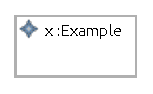
\includegraphics{images/05_library_of_transformations/03_instance_level_transformations/01_plain_objects/class_instance.pdf}
        \caption{$Im_{Class}$ with one object identified as $x$}
        \label{fig:library_of_transformations:instance_level_transformations:plain_objects:visualisation:ecore}
    \end{subfigure}
    \begin{subfigure}{0.45\textwidth}
        \centering
        \input{images/05_library_of_transformations/03_instance_level_transformations/01_plain_objects/class_as_node_type_instance.tikz}
        \caption{$IG_{Class}$ with one node identified as $x$}
        \label{fig:library_of_transformations:instance_level_transformations:plain_objects:visualisation:groove}
    \end{subfigure}
    \caption{Visualisation of the transformation of plain objects typed by regular classes}
    \label{fig:library_of_transformations:instance_level_transformations:plain_objects:visualisation}
\end{figure}

The first transformation that will be defined is a transformation of plain objects of a regular class type. The corresponding type level transformation can be found in \cref{subsec:library_of_transformations:type_level_transformations:regular_classes}. This transformation introduces an arbitrary amount of instances of the class introduced on the type level. First, the definition of the corresponding instance model is given.

\begin{defin}[Instance model $Im_{Class}$]
\label{defin:library_of_transformations:instance_level_transformations:plain_objects:imod_class}
Let $Im_{Class}$ be the instance model containing a set of objects $objects$ which are all typed by class $name$. Furthermore, an injective function $fid$ is defined which maps every object in the set to its corresponding identifier. $Im_{Class}$ is typed by $Tm_{Class}$ (\cref{defin:library_of_transformations:type_level_transformations:regular_classes:tmod_class}) and is defined as:
\begin{align*}
Object =\ &objects \\
\mathrm{ObjectClass} =\ & \begin{cases}
    (ob, name) & \mathrm{if }\ ob \in objects
\end{cases}\\
\mathrm{ObjectId} =\ & \begin{cases}
    (ob, fid(ob)) & \mathrm{if }\ ob \in objects
\end{cases}\\
\mathrm{FieldValue} =\ & \{\} \\
\mathrm{DefaultValue} =\ & \{\}
\end{align*}
\isabellelref{imod_class}{Ecore-GROOVE-Mapping-Library.ClassInstance}
\end{defin}

\begin{thm}[Correctness of $Im_{Class}$]
\label{defin:library_of_transformations:instance_level_transformations:plain_objects:imod_class_correct}
$Im_{Class}$ (\cref{defin:library_of_transformations:instance_level_transformations:plain_objects:imod_class}) is a valid instance model in the sense of \cref{defin:formalisations:ecore_formalisation:instance_models:model_validity}.
\isabellelref{imod_class_correct}{Ecore-GROOVE-Mapping-Library.ClassInstance}
\end{thm}

A visual representation of $Im_{Class}$ with $objects = \{ob\}$ and $fid(ob) = x$ can be seen in \cref{fig:library_of_transformations:instance_level_transformations:plain_objects:visualisation:ecore}. Although this visualisation only shows one object, it is possible to have an arbitrary amount of objects in $Im_{Class}$, as long as they are all typed by the corresponding class introduced on the type level. In the visualisation, the identifier $.\type{Example}$ is used for the class, in correspondence with \cref{fig:library_of_transformations:type_level_transformations:regular_classes:visualisation:ecore} The correctness proof of $Im_{Class}$ is trivial, and therefore not included here. The proof can be found as part of the Isabelle validated proofs.

In order to make composing transformation functions possible, $Im_{Class}$ should be compatible with the instance model it is combined with.

\begin{thm}[Correctness of $\mathrm{combine}(Im, Im_{Class})$]
\label{defin:library_of_transformations:instance_level_transformations:plain_objects:imod_class_combine_correct}
Assume an instance model $Im$ that is valid in the sense of \cref{defin:formalisations:ecore_formalisation:instance_models:model_validity}. Then $Im$ is compatible with $Im_{Class}$ (in the sense of \cref{defin:transformation_framework:instance_models_and_instance_graphs:combining_instance_models:compatibility}) if:
\begin{itemize}
    \item All requirements of \cref{defin:library_of_transformations:type_level_transformations:regular_classes:tmod_class_combine_correct} are met, to ensure the combination of the corresponding type models is valid;
    \item All the objects in $Im_{Class}$ have an (internal and explicit) identity that is not yet used in $Im$.
\end{itemize}
\isabellelref{imod_class_combine_correct}{Ecore-GROOVE-Mapping-Library.ClassInstance}
\end{thm}

\begin{proof}
Use \cref{defin:transformation_framework:instance_models_and_instance_graphs:combining_instance_models:imod_combine_merge_correct}. It is possible to show that all assumptions hold. Now we have shown that $\mathrm{combine}(Im, Im_{Class})$ is consistent in the sense of \cref{defin:formalisations:ecore_formalisation:instance_models:model_validity}.
\end{proof}

Please note that this combination is quite trivial, as the newly introduced objects cannot have fields. This is because they are all typed by the new class type introduced in $Tm_{Class}$. Since this new class type is new by assumption, the existing model cannot have fields defined for the class type.

The definitions and theorems for introducing plain objects of regular classes within Ecore are now complete. 

\subsubsection{Encoding as nodes}

A possible encoding for plain objects in Ecore is using nodes in GROOVE. Each node is typed by the node type that was introduced in $TG_{Class}$, and copies the identifiers set of the objects to the corresponding nodes. The encoding corresponding to $Im_{Class}$ can then be represented as $IG_{Class}$, defined in the following definition:

\begin{defin}[Instance graph $IG_{Class}$]
\label{defin:library_of_transformations:instance_level_transformations:plain_objects:ig_class_as_node_type}
Let $IG_{Class}$ be the instance graph with as nodes the converted $objects$ of $Im_{Class}$ (\cref{defin:library_of_transformations:instance_level_transformations:plain_objects:imod_class}). Furthermore, reuse the injective function $fid$ that maps every object to its identifier. Finally, use the node type introduced in $TG_{Class}$ (\cref{defin:library_of_transformations:type_level_transformations:regular_classes:tg_class_as_node_type}). $IG_{Class}$ is defined typed by $TG_{Class}$ and is defined as:
\begin{align*}
N =\ & objects \\
E =\ & \{\} \\
\mathrm{ident} =\ & \begin{cases}
    (fid(ob), ob) & \mathrm{if }\ ob \in objects
\end{cases}
\end{align*}
with
\begin{align*}
\mathrm{type}_n =\ & \begin{cases}
    (ob, \mathrm{ns\_\!to\_\!list}(name)) & \mathrm{if }\ ob \in objects
\end{cases}
\end{align*}
\isabellelref{ig_class_as_node_type}{Ecore-GROOVE-Mapping-Library.ClassInstance}
\end{defin}

\begin{thm}[Correctness of $IG_{Class}$]
\label{defin:library_of_transformations:instance_level_transformations:plain_objects:ig_class_as_node_type_correct}
$IG_{Class}$ (\cref{defin:library_of_transformations:instance_level_transformations:plain_objects:ig_class_as_node_type}) is a valid instance graph in the sense of \cref{defin:formalisations:groove_formalisation:instance_graphs:instance_graph_validity}.
\isabellelref{ig_class_as_node_type_correct}{Ecore-GROOVE-Mapping-Library.ClassInstance}
\end{thm}

A visual representation of $IG_{Class}$ with $objects = \{ob\}$ and $fid(ob) = x$ can be seen in \cref{fig:library_of_transformations:instance_level_transformations:plain_objects:visualisation:groove}. Like the previous example for the Ecore instance model, only one node is shown here, but multiple nodes can be introduced at once if there are more objects in the $objects$ set. As shown in the definition, the node type identified by $\type{Example}$ is used to type all the nodes, in correspondence with \cref{fig:library_of_transformations:type_level_transformations:regular_classes:visualisation:groove}. The correctness proof of $IG_{Class}$ is trivial, and therefore not included here. The proof can be found as part of the Isabelle validated proofs.

In order to make composing transformation functions possible, $IG_{Class}$ should be compatible with the instance graph it is combined with.

\begin{thm}[Correctness of $\mathrm{combine}(IG, IG_{Class})$]
\label{defin:library_of_transformations:instance_level_transformations:plain_objects:ig_class_as_node_type_combine_correct}
Assume an instance graph $IG$ that is valid in the sense of \cref{defin:formalisations:groove_formalisation:instance_graphs:instance_graph_validity}. Then $IG$ is compatible with $IG_{Class}$ (in the sense of \cref{defin:transformation_framework:instance_models_and_instance_graphs:combining_instance_graphs:compatibility}) if:
\begin{itemize}
    \item All requirements of \cref{defin:library_of_transformations:type_level_transformations:regular_classes:tg_class_as_node_type_combine_correct} are met, to ensure the combination of the corresponding type graphs is valid;
    \item All the nodes in $IG_{Class}$ have an (internal and explicit) identity that is not yet used in $IG$.
\end{itemize}
\isabellelref{ig_class_as_node_type_combine_correct}{Ecore-GROOVE-Mapping-Library.ClassInstance}
\end{thm}

\begin{proof}
Use \cref{defin:transformation_framework:instance_models_and_instance_graphs:combining_instance_graphs:ig_combine_merge_correct}. It is possible to show that all assumptions hold. Now we have shown that $\mathrm{combine}(IG, IG_{Class})$ is valid in the sense of \cref{defin:formalisations:groove_formalisation:instance_graphs:instance_graph_validity}.
\end{proof}

The next definitions define the transformation function from $Im_{Class}$ to $IG_{Class}$:

\begin{defin}[Transformation function $f_{Class}$]
\label{defin:library_of_transformations:instance_level_transformations:plain_objects:imod_class_to_ig_class_as_node_type}
The transformation function $f_{Class}(Im)$ is defined as:
\begin{align*}
N =\ & Object_{Im} \\
E =\ & \{\} \\
\mathrm{ident} =\ & \begin{cases}
    (fid(ob), ob) & \mathrm{if }\ ob \in Object_{Im}
\end{cases}
\end{align*}
with
\begin{align*}
\mathrm{type}_n =\ & \begin{cases}
    (ob, \mathrm{ns\_\!to\_\!list}(name)) & \mathrm{if }\ ob \in Object_{Im}
\end{cases}
\end{align*}
\isabellelref{imod_class_to_ig_class_as_node_type}{Ecore-GROOVE-Mapping-Library.ClassInstance}
\end{defin}

\begin{thm}[Correctness of $f_{Class}$]
\label{defin:library_of_transformations:instance_level_transformations:plain_objects:imod_class_to_ig_class_as_node_type_func}
$f_{Class}(Im)$ (\cref{defin:library_of_transformations:instance_level_transformations:plain_objects:imod_class_to_ig_class_as_node_type}) is a valid transformation function in the sense of \cref{defin:transformation_framework:instance_models_and_instance_graphs:combining_transformation_functions:transformation_function_instance_model_instance_graph} transforming $Im_{Class}$ into $IG_{Class}$.
\isabellelref{imod_class_to_ig_class_as_node_type_func}{Ecore-GROOVE-Mapping-Library.ClassInstance}
\end{thm}

The proof of the correctness of $f_{Class}$ will not be included here. Instead, it can be found in the validated Isabelle theories. The proof is quite trivial, as extending $Im$ can only add extra objects, but not remove the existing ones.

Finally, to complete the transformation, the transformation function that transforms $IG_{Class}$ into $Im_{Class}$ is defined:

\begin{defin}[Transformation function $f'_{Class}$]
\label{defin:library_of_transformations:instance_level_transformations:plain_objects:ig_class_as_node_type_to_imod_class}
The transformation function $f'_{Class}(IG)$ is defined as:
\begin{align*}
Object =\ &N_{IG} \\
\mathrm{ObjectClass} =\ & \begin{cases}
    (ob, name) & \mathrm{if }\ ob \in N_{IG}
\end{cases}\\
\mathrm{ObjectId} =\ & \begin{cases}
    (ob, fid(ob)) & \mathrm{if }\ ob \in N_{IG}
\end{cases}\\
\mathrm{FieldValue} =\ & \{\} \\
\mathrm{DefaultValue} =\ & \{\}
\end{align*}
\isabellelref{ig_class_as_node_type_to_imod_class}{Ecore-GROOVE-Mapping-Library.ClassInstance}
\end{defin}

\begin{thm}[Correctness of $f'_{Class}$]
\label{defin:library_of_transformations:instance_level_transformations:plain_objects:ig_class_as_node_type_to_tmod_class_func}
$f'_{Class}(IG)$ (\cref{defin:library_of_transformations:instance_level_transformations:plain_objects:ig_class_as_node_type_to_imod_class}) is a valid transformation function in the sense of \cref{defin:transformation_framework:instance_models_and_instance_graphs:combining_transformation_functions:transformation_function_instance_graph_instance_model} transforming $IG_{Class}$ into $Im_{Class}$.
\isabellelref{ig_class_as_node_type_to_imod_class_func}{Ecore-GROOVE-Mapping-Library.ClassInstance}
\end{thm}

Once more, the correctness proof is not included here but can be found in the validated Isabelle proofs of this thesis.
\subsection{Abstract classes}
\label{subsec:library_of_transformations:instance_level_transformations:abstract_classes}

In this section, the instance level transformation corresponding to the type level transformation of abstract classes is discussed. The type level transformation of abstract class types can be found in \cref{subsec:library_of_transformations:type_level_transformations:abstract_classes}.

Informally speaking, it is quite weird to think about the transformation of abstract classes on the instance level, as abstract classes cannot have instances. The transformation here is included for completeness, to allow for adding abstract types while working with transformations on the type level. In practice, the instance level will consist of the empty instance model and empty instance graph, showing that after adding an abstract class on the type level, instances of the type model will still be valid.

First, the corresponding instance model is introduced.

\begin{defin}[Instance model $Im_{AbsClass}$]
\label{defin:library_of_transformations:instance_level_transformations:abstract_classes:imod_abstract_class}
Let $Im_{AbsClass}$ be the empty instance model $Im_\epsilon$ (\cref{defin:transformation_framework:instance_models_and_instance_graphs:combining_instance_models:empty_instance_model}), except that it is typed by the type model $Tm_{AbsClass}$ (\cref{defin:library_of_transformations:type_level_transformations:abstract_classes:tmod_abstract_class}).
\isabellelref{imod_abstract_class}{Ecore-GROOVE-Mapping-Library.AbstractClassInstance}
\end{defin}

\begin{thm}[Correctness of $Im_{AbsClass}$]
\label{defin:library_of_transformations:instance_level_transformations:abstract_classes:imod_abstract_class_correct}
$Im_{AbsClass}$ (\cref{defin:library_of_transformations:instance_level_transformations:abstract_classes:imod_abstract_class}) is a valid instance model in the sense of \cref{defin:formalisations:ecore_formalisation:instance_models:model_validity}.
\isabellelref{imod_abstract_class_correct}{Ecore-GROOVE-Mapping-Library.AbstractClassInstance}
\end{thm}

Since $Im_{AbsClass}$ does not define any objects, there is no need for a visual representation. However, in order to make composing transformation functions possible, $Im_{AbsClass}$ should still be compatible with the instance model it is combined with.

\begin{thm}[Correctness of $\mathrm{combine}(Im, Im_{AbsClass})$]
\label{defin:library_of_transformations:instance_level_transformations:abstract_classes:imod_abstract_class_combine_correct}
Assume an instance model $Im$ that is valid in the sense of \cref{defin:formalisations:ecore_formalisation:instance_models:model_validity}. Then $Im$ is compatible with $Im_{AbsClass}$ (in the sense of \cref{defin:transformation_framework:instance_models_and_instance_graphs:combining_instance_models:compatibility}) if:
\begin{itemize}
    \item All requirements of \cref{defin:library_of_transformations:type_level_transformations:abstract_classes:tmod_abstract_class_combine_correct} are met, to ensure the combination of the corresponding type models is valid.
\end{itemize}
\isabellelref{imod_abstract_class_combine_correct}{Ecore-GROOVE-Mapping-Library.AbstractClassInstance}
\end{thm}

\begin{proof}
Use \cref{defin:transformation_framework:instance_models_and_instance_graphs:combining_instance_models:imod_combine_merge_correct}. It is possible to show that all assumptions hold. Now we have shown that $\mathrm{combine}(Im, Im_{AbsClass})$ is consistent in the sense of \cref{defin:formalisations:ecore_formalisation:instance_models:model_validity}.
\end{proof}

The definitions and theorems for the Ecore instance model corresponding to $Tm_{AbsClass}$ are now complete. 

\subsubsection{The node type encoding}

As has been shown earlier, an possible encoding for abstract class types is by introducing an abstract node type. This has been done in $TG_{AbsClass}$. Like the Ecore instance model, the GROOVE instance graph is also empty, because abstract node types cannot be instantiated. This gives rise to $IG_{AbsClass}$, which is defined as follows:

\begin{defin}[Instance graph $IG_{AbsClass}$]
\label{defin:library_of_transformations:instance_level_transformations:abstract_classes:ig_abstract_class_as_node_type}
Let $IG_{AbsClass}$ be the empty instance graph $IG_\epsilon$ (\cref{defin:transformation_framework:instance_models_and_instance_graphs:combining_instance_graphs:empty_instance_graph}), except that it is typed by the type graph $TG_{AbsClass}$ (\cref{defin:library_of_transformations:type_level_transformations:abstract_classes:tg_abstract_class_as_node_type}).
\isabellelref{ig_abstract_class_as_node_type}{Ecore-GROOVE-Mapping-Library.AbstractClassInstance}
\end{defin}

\begin{thm}[Correctness of $IG_{AbsClass}$]
\label{defin:library_of_transformations:instance_level_transformations:abstract_classes:ig_class_as_node_type_correct}
$IG_{AbsClass}$ (\cref{defin:library_of_transformations:instance_level_transformations:abstract_classes:ig_abstract_class_as_node_type}) is a valid instance graph in the sense of \cref{defin:formalisations:groove_formalisation:instance_graphs:instance_graph_validity}.
\isabellelref{ig_abstract_class_as_node_type_correct}{Ecore-GROOVE-Mapping-Library.AbstractClassInstance}
\end{thm}

In order to make composing transformation functions possible, $IG_{AbsClass}$ should be compatible with the instance graph it is combined with.

\begin{thm}[Correctness of $\mathrm{combine}(IG, IG_{AbsClass})$]
\label{defin:library_of_transformations:instance_level_transformations:abstract_classes:ig_abstract_class_as_node_type_combine_correct}
Assume an instance graph $IG$ that is valid in the sense of \cref{defin:formalisations:groove_formalisation:instance_graphs:instance_graph_validity}. Then $IG$ is compatible with $IG_{AbsClass}$ (in the sense of \cref{defin:transformation_framework:instance_models_and_instance_graphs:combining_instance_graphs:compatibility}) if:
\begin{itemize}
    \item All requirements of \cref{defin:library_of_transformations:type_level_transformations:abstract_classes:tg_abstract_class_as_node_type_combine_correct} are met, to ensure the combination of the corresponding type graphs is valid.
\end{itemize}
\isabellelref{ig_abstract_class_as_node_type_combine_correct}{Ecore-GROOVE-Mapping-Library.AbstractClassInstance}
\end{thm}

\begin{proof}
Use \cref{defin:transformation_framework:instance_models_and_instance_graphs:combining_instance_graphs:ig_combine_merge_correct}. It is possible to show that all assumptions hold. Now we have shown that $\mathrm{combine}(IG, IG_{AbsClass})$ is valid in the sense of \cref{defin:formalisations:groove_formalisation:instance_graphs:instance_graph_validity}.
\end{proof}

The next definitions define the transformation function from $Im_{AbsClass}$ to $IG_{AbsClass}$:

\begin{defin}[Transformation function $f_{AbsClass}$]
\label{defin:library_of_transformations:instance_level_transformations:abstract_classes:imod_abstract_class_to_ig_abstract_class_as_node_type}
The transformation function $f_{AbsClass}(Im)$ is defined as the function that always outputs the empty instance graph $IG_\epsilon$ (\cref{defin:transformation_framework:instance_models_and_instance_graphs:combining_instance_graphs:empty_instance_graph}), except that it is typed by $TG_{AbsClass}$.
\isabellelref{imod_abstract_class_to_ig_abstract_class_as_node_type}{Ecore-GROOVE-Mapping-Library.AbstractClassInstance}
\end{defin}

\begin{thm}[Correctness of $f_{AbsClass}$]
\label{defin:library_of_transformations:instance_level_transformations:abstract_classes:imod_abstract_class_to_ig_abstract_class_as_node_type_func}
$f_{AbsClass}(Im)$ (\cref{defin:library_of_transformations:instance_level_transformations:abstract_classes:imod_abstract_class_to_ig_abstract_class_as_node_type}) is a valid transformation function in the sense of \cref{defin:transformation_framework:instance_models_and_instance_graphs:combining_transformation_functions:transformation_function_instance_model_instance_graph} transforming $Im_{AbsClass}$ into $IG_{AbsClass}$.
\isabellelref{imod_abstract_class_to_ig_abstract_class_as_node_type_func}{Ecore-GROOVE-Mapping-Library.AbstractClassInstance}
\end{thm}

The proof of the correctness of $f_{AbsClass}$ will not be included here. Instead, it can be found in the validated Isabelle theories. Obviously, the proof is trivial, as the function does not do any conversion. It does just output the empty instance model.

Finally, to complete the transformation, the transformation function that transforms $IG_{AbsClass}$ into $Im_{AbsClass}$ is defined:

\begin{defin}[Transformation function $f'_{AbsClass}$]
\label{defin:library_of_transformations:instance_level_transformations:abstract_classes:ig_abstract_class_as_node_type_to_imod_abstract_class}
The transformation function $f'_{AbsClass}(IG)$ is defined as the function that always outputs the empty instance model $Im_\epsilon$ (\cref{defin:transformation_framework:instance_models_and_instance_graphs:combining_instance_models:empty_instance_model}), except that it is typed by $Tm_{AbsClass}$.
\isabellelref{ig_abstract_class_as_node_type_to_imod_abstract_class}{Ecore-GROOVE-Mapping-Library.AbstractClassInstance}
\end{defin}

\begin{thm}[Correctness of $f'_{AbsClass}$]
\label{defin:library_of_transformations:instance_level_transformations:abstract_classes:ig_abstract_class_as_node_type_to_imod_abstract_class_func}
$f'_{AbsClass}(IG)$ (\cref{defin:library_of_transformations:instance_level_transformations:abstract_classes:ig_abstract_class_as_node_type_to_imod_abstract_class}) is a valid transformation function in the sense of \cref{defin:transformation_framework:instance_models_and_instance_graphs:combining_transformation_functions:transformation_function_instance_graph_instance_model} transforming $IG_{AbsClass}$ into $Im_{AbsClass}$.
\isabellelref{ig_abstract_class_as_node_type_to_imod_abstract_class_func}{Ecore-GROOVE-Mapping-Library.AbstractClassInstance}
\end{thm}

Once more, the correctness proof is not included here but can be found in the validated Isabelle proofs of this thesis.
\subsection{Plain objects typed by a subclass}
\label{subsec:library_of_transformations:instance_level_transformations:objects_of_subtype}

\begin{figure}
    \centering
    \begin{subfigure}{0.45\textwidth}
        \centering
        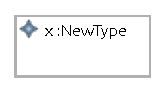
\includegraphics{images/05_library_of_transformations/03_instance_level_transformations/03_objects_of_subtype/subclass_instance.pdf}
        \caption{$Im_{Subclass}$ with one object identified as $x$}
        \label{fig:library_of_transformations:instance_level_transformations:objects_of_subtype:visualisation:ecore}
    \end{subfigure}
    \begin{subfigure}{0.45\textwidth}
        \centering
        \input{images/05_library_of_transformations/03_instance_level_transformations/03_objects_of_subtype/subclass_as_node_type_instance.tikz}
        \caption{$IG_{Subclass}$ with one node identified as $x$}
        \label{fig:library_of_transformations:instance_level_transformations:objects_of_subtype:visualisation:groove}
    \end{subfigure}
    \caption{Visualisation of the transformation of objects typed by a subclass}
    \label{fig:library_of_transformations:instance_level_transformations:objects_of_subtype:visualisation}
\end{figure}

In this section, the transformation of plain objects typed by a regular subclass is discussed. The corresponding type level transformation can be found in \cref{subsec:library_of_transformations:type_level_transformations:regular_subclasses}. This transformation is very similar to the the transformation of plain objects discussed in \cref{subsec:library_of_transformations:instance_level_transformations:plain_objects}. Like that transformation, it is possible to introduce an arbitrary amount of instances of the subclass introduced on the type level. First, the definition of the corresponding instance model is given.

\begin{defin}[Instance model $Im_{Subclass}$]
\label{defin:library_of_transformations:instance_level_transformations:objects_of_subtype:imod_subclass}
Let $Im_{Subclass}$ be the instance model containing a set of objects $objects$ which are all typed by subclass $name$, which extends class $supertype$. Furthermore, an injective function $fid$ is defined which maps every object in the set to its corresponding identifier. $Im_{Subclass}$ is typed by $Tm_{Subclass}$ (\cref{defin:library_of_transformations:type_level_transformations:regular_subclasses:tmod_subclass}) and is defined as:
\begin{align*}
Object =\ &objects \\
\mathrm{ObjectClass} =\ & \begin{cases}
    (ob, name) & \mathrm{if }\ ob \in objects
\end{cases}\\
\mathrm{ObjectId} =\ & \begin{cases}
    (ob, fid(ob)) & \mathrm{if }\ ob \in objects
\end{cases}\\
\mathrm{FieldValue} =\ & \{\} \\
\mathrm{DefaultValue} =\ & \{\}
\end{align*}
\isabellelref{imod_subclass}{Ecore-GROOVE-Mapping-Library.SubclassInstance}
\end{defin}

\begin{thm}[Correctness of $Im_{Subclass}$]
\label{defin:library_of_transformations:instance_level_transformations:objects_of_subtype:imod_subclass_correct}
$Im_{Subclass}$ (\cref{defin:library_of_transformations:instance_level_transformations:objects_of_subtype:imod_subclass}) is a valid instance model in the sense of \cref{defin:formalisations:ecore_formalisation:instance_models:model_validity}.
\isabellelref{imod_subclass_correct}{Ecore-GROOVE-Mapping-Library.SubclassInstance}
\end{thm}

A visual representation of $Im_{Subclass}$ with $objects = \{ob\}$ and $fid(ob) = x$ can be seen in \cref{fig:library_of_transformations:instance_level_transformations:objects_of_subtype:visualisation:ecore}. Although this visualisation only shows one object, it is possible to have an arbitrary amount of objects in $Im_{Subclass}$, as long as they are all typed by the corresponding class introduced on the type level. In the visualisation, the identifier $.\type{NewType}$ is used for the class, in correspondence with \cref{fig:library_of_transformations:type_level_transformations:regular_subclasses:visualisation:ecore} The correctness proof of $Im_{Subclass}$ is trivial, and therefore not included here. The proof can be found as part of the Isabelle validated proofs.

In order to make composing transformation functions possible, $Im_{Subclass}$ should be compatible with the instance model it is combined with.

\begin{thm}[Correctness of $\mathrm{combine}(Im, Im_{Subclass})$]
\label{defin:library_of_transformations:instance_level_transformations:objects_of_subtype:imod_subclass_combine_correct}
Assume an instance model $Im$ that is valid in the sense of \cref{defin:formalisations:ecore_formalisation:instance_models:model_validity}. Then $Im$ is compatible with $Im_{Subclass}$ (in the sense of \cref{defin:transformation_framework:instance_models_and_instance_graphs:combining_instance_models:compatibility}) if:
\begin{itemize}
    \item All requirements of \cref{defin:library_of_transformations:type_level_transformations:regular_subclasses:tmod_subclass_combine_correct} are met, to ensure the combination of the corresponding type models is valid;
    \item All the objects in $Im_{Subclass}$ have an (internal and explicit) identity that is not yet used in $Im$;
    \item $Im$ is not typed by a type model that defines any fields for the $supertype$ class.
\end{itemize}
\isabellelref{imod_subclass_combine_correct}{Ecore-GROOVE-Mapping-Library.SubclassInstance}
\end{thm}

\begin{proof}
Use \cref{defin:transformation_framework:instance_models_and_instance_graphs:combining_instance_models:imod_combine_merge_correct}. It is possible to show that all assumptions hold. Now we have shown that $\mathrm{combine}(Im, Im_{Subclass})$ is consistent in the sense of \cref{defin:formalisations:ecore_formalisation:instance_models:model_validity}.
\end{proof}

Please note that in this case, it has been made explicit that the new objects introduced do not have any fields defined. This is by ensuring the supertype does not define any fields. The new subclass does not have fields itself, as it cannot have existed in the combined type model.

The definitions and theorems for introducing plain objects of regular subclasses within Ecore are now complete. 

\subsubsection{Encoding as nodes}

As was the case with plain objects of regular classes, a possible encoding for plain objects of subclasses in Ecore is using nodes in GROOVE. Each node is typed by the node type that was introduced in $TG_{Subclass}$, and copies the identifiers set of the objects to the corresponding nodes. The encoding corresponding to $Im_{Subclass}$ can then be represented as $IG_{Subclass}$, defined in the following definition:

\begin{defin}[Instance graph $IG_{Subclass}$]
\label{defin:library_of_transformations:instance_level_transformations:objects_of_subtype:ig_subclass_as_node_type}
Let $IG_{Subclass}$ be the instance graph with as nodes the converted $objects$ of $Im_{Subclass}$ (\cref{defin:library_of_transformations:instance_level_transformations:objects_of_subtype:imod_subclass}). Furthermore, reuse the injective function $fid$ that maps every object to its identifier. Finally, use the node type $name$ introduced in $TG_{Subclass}$, that extends the $supertype$ node type. (\cref{defin:library_of_transformations:type_level_transformations:regular_classes:tg_class_as_node_type}). $IG_{Subclass}$ is defined typed by $TG_{Subclass}$ and is defined as:
\begin{align*}
N =\ & objects \\
E =\ & \{\} \\
\mathrm{ident} =\ & \begin{cases}
    (fid(ob), ob) & \mathrm{if }\ ob \in objects
\end{cases}
\end{align*}
with
\begin{align*}
\mathrm{type}_n =\ & \begin{cases}
    (ob, \mathrm{ns\_\!to\_\!list}(name)) & \mathrm{if }\ ob \in objects
\end{cases}
\end{align*}
\isabellelref{ig_subclass_as_node_type}{Ecore-GROOVE-Mapping-Library.SubclassInstance}
\end{defin}

\begin{thm}[Correctness of $IG_{Subclass}$]
\label{defin:library_of_transformations:instance_level_transformations:objects_of_subtype:ig_subclass_as_node_type_correct}
$IG_{Subclass}$ (\cref{defin:library_of_transformations:instance_level_transformations:objects_of_subtype:ig_subclass_as_node_type}) is a valid instance graph in the sense of \cref{defin:formalisations:groove_formalisation:instance_graphs:instance_graph_validity}.
\isabellelref{ig_subclass_as_node_type_correct}{Ecore-GROOVE-Mapping-Library.SubclassInstance}
\end{thm}

A visual representation of $IG_{Subclass}$ with $objects = \{ob\}$ and $fid(ob) = x$ can be seen in \cref{fig:library_of_transformations:instance_level_transformations:objects_of_subtype:visualisation:groove}. Like the previous example for the Ecore instance model, only one node is shown here, but multiple nodes can be introduced at once if there are more objects in the $objects$ set. As shown in the definition, the node type identified by $\type{NewType}$ is used to type all the nodes, in correspondence with \cref{fig:library_of_transformations:type_level_transformations:regular_subclasses:visualisation:groove}. The correctness proof of $IG_{Subclass}$ is trivial, and therefore not included here. The proof can be found as part of the Isabelle validated proofs.

In order to make composing transformation functions possible, $IG_{Subclass}$ should be compatible with the instance graph it is combined with.

\begin{thm}[Correctness of $\mathrm{combine}(IG, IG_{Subclass})$]
\label{defin:library_of_transformations:instance_level_transformations:objects_of_subtype:ig_subclass_as_node_type_combine_correct}
Assume an instance graph $IG$ that is valid in the sense of \cref{defin:formalisations:groove_formalisation:instance_graphs:instance_graph_validity}. Then $IG$ is compatible with $IG_{Subclass}$ (in the sense of \cref{defin:transformation_framework:instance_models_and_instance_graphs:combining_instance_graphs:compatibility}) if:
\begin{itemize}
    \item All requirements of \cref{defin:library_of_transformations:type_level_transformations:regular_subclasses:tg_subclass_as_node_type_combine_correct} are met, to ensure the combination of the corresponding type graphs is valid;
    \item All the nodes in $IG_{Subclass}$ have an (internal and explicit) identity that is not yet used in $IG$;
    \item There are no edge types from or to the $supertype$ node type, this includes edges from and to types that $supertype$ inherits from.
\end{itemize}
\isabellelref{ig_subclass_as_node_type_combine_correct}{Ecore-GROOVE-Mapping-Library.SubclassInstance}
\end{thm}

\begin{proof}
Use \cref{defin:transformation_framework:instance_models_and_instance_graphs:combining_instance_graphs:ig_combine_merge_correct}. It is possible to show that all assumptions hold. Now we have shown that $\mathrm{combine}(IG, IG_{Subclass})$ is valid in the sense of \cref{defin:formalisations:groove_formalisation:instance_graphs:instance_graph_validity}.
\end{proof}

Like the correctness for the Ecore instance model, validity is guaranteed here by assuming there exist no edge types from and to the $supertype$ node type.

The next definitions define the transformation function from $Im_{Subclass}$ to $IG_{Subclass}$:

\begin{defin}[Transformation function $f_{Subclass}$]
\label{defin:library_of_transformations:instance_level_transformations:objects_of_subtype:imod_subclass_to_ig_subclass_as_node_type}
The transformation function $f_{Subclass}(Im)$ is defined as:
\begin{align*}
N =\ & Object_{Im} \\
E =\ & \{\} \\
\mathrm{ident} =\ & \begin{cases}
    (fid(ob), ob) & \mathrm{if }\ ob \in Object_{Im}
\end{cases}
\end{align*}
with
\begin{align*}
\mathrm{type}_n =\ & \begin{cases}
    (ob, \mathrm{ns\_\!to\_\!list}(name)) & \mathrm{if }\ ob \in Object_{Im}
\end{cases}
\end{align*}
\isabellelref{imod_subclass_to_ig_subclass_as_node_type}{Ecore-GROOVE-Mapping-Library.SubclassInstance}
\end{defin}

\begin{thm}[Correctness of $f_{Subclass}$]
\label{defin:library_of_transformations:instance_level_transformations:objects_of_subtype:imod_subclass_to_ig_subclass_as_node_type_func}
$f_{Subclass}(Im)$ (\cref{defin:library_of_transformations:instance_level_transformations:objects_of_subtype:imod_subclass_to_ig_subclass_as_node_type}) is a valid transformation function in the sense of \cref{defin:transformation_framework:instance_models_and_instance_graphs:combining_transformation_functions:transformation_function_instance_model_instance_graph} transforming $Im_{Subclass}$ into $IG_{Subclass}$.
\isabellelref{imod_subclass_to_ig_subclass_as_node_type_func}{Ecore-GROOVE-Mapping-Library.SubclassInstance}
\end{thm}

The proof of the correctness of $f_{Subclass}$ will not be included here. Instead, it can be found in the validated Isabelle theories. The proof is quite trivial, as extending $Im$ can only add extra objects, but not remove the existing ones.

Finally, to complete the transformation, the transformation function that transforms $IG_{Subclass}$ into $Im_{Subclass}$ is defined:

\begin{defin}[Transformation function $f'_{Subclass}$]
\label{defin:library_of_transformations:instance_level_transformations:objects_of_subtype:ig_subclass_as_node_type_to_imod_subclass}
The transformation function $f'_{Subclass}(IG)$ is defined as:
\begin{align*}
Object =\ &N_{IG} \\
\mathrm{ObjectClass} =\ & \begin{cases}
    (ob, name) & \mathrm{if }\ ob \in N_{IG}
\end{cases}\\
\mathrm{ObjectId} =\ & \begin{cases}
    (ob, fid(ob)) & \mathrm{if }\ ob \in N_{IG}
\end{cases}\\
\mathrm{FieldValue} =\ & \{\} \\
\mathrm{DefaultValue} =\ & \{\}
\end{align*}
\isabellelref{ig_subclass_as_node_type_to_imod_subclass}{Ecore-GROOVE-Mapping-Library.SubclassInstance}
\end{defin}

\begin{thm}[Correctness of $f'_{Subclass}$]
\label{defin:library_of_transformations:instance_level_transformations:objects_of_subtype:ig_subclass_as_node_type_to_imod_subclass_func}
$f'_{Subclass}(IG)$ (\cref{defin:library_of_transformations:instance_level_transformations:objects_of_subtype:ig_subclass_as_node_type_to_imod_subclass}) is a valid transformation function in the sense of \cref{defin:transformation_framework:instance_models_and_instance_graphs:combining_transformation_functions:transformation_function_instance_graph_instance_model} transforming $IG_{Subclass}$ into $Im_{Subclass}$.
\isabellelref{ig_subclass_as_node_type_to_imod_subclass_func}{Ecore-GROOVE-Mapping-Library.SubclassInstance}
\end{thm}

Once more, the correctness proof is not included here but can be found in the validated Isabelle proofs of this thesis.
\subsection{Enumeration values}
\label{subsec:library_of_transformations:instance_level_transformations:enumeration_values}

\begin{figure}
    \centering
    \begin{subfigure}{0.45\textwidth}
        \centering
        \input{images/05_library_of_transformations/03_instance_level_transformations/04_enumeration_values/enum_as_node_types_values.tikz}
        \caption{$IG_{EnumNodes}$ corresponding to $TG_{EnumNodes}$}
        \label{fig:library_of_transformations:instance_level_transformations:enumeration_values:visualisation:groove_nodes}
    \end{subfigure}
    \begin{subfigure}{0.45\textwidth}
        \centering
        \input{images/05_library_of_transformations/03_instance_level_transformations/04_enumeration_values/enum_as_flags_values.tikz}
        \caption{$IG_{EnumFlags}$ corresponding to $TG_{EnumFlags}$}
        \label{fig:library_of_transformations:instance_level_transformations:enumeration_values:visualisation:groove_flags}
    \end{subfigure}
    \caption{Visualisation of the transformation of enumeration values corresponding to an enumeration type}
    \label{fig:library_of_transformations:instance_level_transformations:enumeration_values:visualisation}
\end{figure}

This section defines the transformation of enumeration values belonging to an enumeration type on the type level. The corresponding type level transformation can be found in \cref{subsec:library_of_transformations:type_level_transformations:enumeration_types}. This transformation introduces new nodes in an instance graph that correspond to the values of an enumeration type. Within an instance model, nothing new needs to be introduced, and there the empty instance model is used once more.

First, the instance model corresponding to $Tm_{Enum}$ is defined.

\begin{defin}[Instance model $Im_{Enum}$]
\label{defin:library_of_transformations:instance_level_transformations:enumeration_values:imod_enum}
Let $Im_{Enum}$ be the empty instance model $Im_\epsilon$ (\cref{defin:transformation_framework:instance_models_and_instance_graphs:combining_instance_models:empty_instance_model}), except that it is typed by the type model $Tm_{Enum}$ (\cref{defin:library_of_transformations:type_level_transformations:enumeration_types:tmod_enum}).
\isabellelref{imod_enum}{Ecore-GROOVE-Mapping-Library.EnumInstance}
\end{defin}

\begin{thm}[Correctness of $Im_{Enum}$]
\label{defin:library_of_transformations:instance_level_transformations:enumeration_values:imod_enum_correct}
$Im_{Enum}$ (\cref{defin:library_of_transformations:instance_level_transformations:enumeration_values:imod_enum}) is a valid instance model in the sense of \cref{defin:formalisations:ecore_formalisation:instance_models:model_validity}.
\isabellelref{imod_enum_correct}{Ecore-GROOVE-Mapping-Library.EnumInstance}
\end{thm}

Since the instance model corresponding to the transformation of enumeration values does not define any objects, there is no visual representation needed. Moreover, the correctness proof of $Im_{Enum}$ is trivial, and therefore not included here. The proof can be found as part of the Isabelle validated proofs.

In order to make composing transformation functions possible, $Im_{Enum}$ should be compatible with the instance model it is combined with.

\begin{thm}[Correctness of $\mathrm{combine}(Im, Im_{Enum})$]
\label{defin:library_of_transformations:instance_level_transformations:enumeration_values:imod_enum_combine_correct}
Assume an instance model $Im$ that is valid in the sense of \cref{defin:formalisations:ecore_formalisation:instance_models:model_validity}. Then $Im$ is compatible with $Im_{Enum}$ (in the sense of \cref{defin:transformation_framework:instance_models_and_instance_graphs:combining_instance_models:compatibility}) if:
\begin{itemize}
    \item All requirements of \cref{defin:library_of_transformations:type_level_transformations:enumeration_types:tmod_enum_combine_correct} are met, to ensure the combination of the corresponding type models is valid.
\end{itemize}
\isabellelref{imod_enum_combine_correct}{Ecore-GROOVE-Mapping-Library.EnumInstance}
\end{thm}

\begin{proof}
Use \cref{defin:transformation_framework:instance_models_and_instance_graphs:combining_instance_models:imod_combine_merge_correct}. It is possible to show that all assumptions hold. Now we have shown that $\mathrm{combine}(Im, Im_{Enum})$ is consistent in the sense of \cref{defin:formalisations:ecore_formalisation:instance_models:model_validity}.
\end{proof}

Please note that this combination is trivial, as the instance model is empty. However, on the instance graph level, more complex definitions are used.

The definitions and theorems for introducing plain objects of regular classes within Ecore are now complete. 

\subsubsection{Encoding of node type values as nodes}

Section \cref{subsec:library_of_transformations:type_level_transformations:enumeration_types} has shown two possible encodings of an enumeration type in GROOVE. Both encodings require a different definition on the instance level. In the case that an enumeration type is encoded as node types, the enumeration values will be nodes typed by these node types, one node for each value of the enumeration type. This gives rise to an instance graph $IG_{EnumNodes}$, defined in the following definition:

\begin{defin}[Instance graph $IG_{EnumNodes}$]
\label{defin:library_of_transformations:instance_level_transformations:enumeration_values:ig_enum_as_node_types}
Let $IG_{EnumNodes}$ be the instance graph corresponding $TG_{EnumNodes}$ (\cref{defin:library_of_transformations:type_level_transformations:enumeration_types:tg_enum_as_node_types}). $IG_{EnumNodes}$ defines a node for each possible value of the enumeration type encoded by $TG_{EnumNodes}$. Each of these nodes is typed by its corresponding node type. Furthermore, the function $fob$ and $fib$ are defined. $fob$ converts each value of the enumeration type to its internal node identity. $fid$ maps each value of the enumeration type to an explicit identity. $IG_{EnumNodes}$ is defined typed by $TG_{EnumNodes}$ and is defined as:
\begin{align*}
N =\ & \{fob(v) \mid v \in values \} \\
E =\ & \{\} \\
\mathrm{ident} =\ & \begin{cases}
    (fid(v), fob(v)) & \mathrm{if }\ v \in values
\end{cases}
\end{align*}
with
\begin{align*}
\mathrm{type}_n =\ & \begin{cases}
    (v, \mathrm{ns\_\!to\_\!list}(name) \append \langle v \rangle) & \mathrm{if }\ v \in values
\end{cases}
\end{align*}
\isabellelref{ig_enum_as_node_types}{Ecore-GROOVE-Mapping-Library.EnumInstance}
\end{defin}

\begin{thm}[Correctness of $IG_{EnumNodes}$]
\label{defin:library_of_transformations:instance_level_transformations:enumeration_values:ig_enum_as_node_types_correct}
$IG_{EnumNodes}$ (\cref{defin:library_of_transformations:instance_level_transformations:enumeration_values:ig_enum_as_node_types}) is a valid instance graph in the sense of \cref{defin:formalisations:groove_formalisation:instance_graphs:instance_graph_validity}.
\isabellelref{ig_enum_as_node_types_correct}{Ecore-GROOVE-Mapping-Library.EnumInstance}
\end{thm}

A visual representation of $IG_{EnumNodes}$ with $.\type{Example}$ as identifier for the encoded enumeration type and $\type{OPTION\_A}$, $\type{OPTION\_B}$ and $\type{OPTION\_C}$ as its values can be seen in \cref{fig:library_of_transformations:instance_level_transformations:enumeration_values:visualisation:groove_nodes}. In this representation, it can also be seen that each values has its corresponding identifier, with $fid(\type{OPTION\_A}) = ExampleOptionA$, $fid(\type{OPTION\_B}) = ExampleOptionB$ and $fid(\type{OPTION\_C}) = ExampleOptionC$. Furthermore, the instances shown here correspond to the visual representation shown in \cref{fig:library_of_transformations:type_level_transformations:enumeration_types:visualisation:groove_nodes}. The correctness proof of $IG_{EnumNodes}$ is trivial, and therefore not included here. The proof can be found as part of the Isabelle validated proofs.

In order to make composing transformation functions possible, $IG_{EnumNodes}$ should be compatible with the instance graph it is combined with.

\begin{thm}[Correctness of $\mathrm{combine}(IG, IG_{EnumNodes})$]
\label{defin:library_of_transformations:instance_level_transformations:enumeration_values:ig_enum_as_node_types_combine_correct}
Assume an instance graph $IG$ that is valid in the sense of \cref{defin:formalisations:groove_formalisation:instance_graphs:instance_graph_validity}. Then $IG$ is compatible with $IG_{EnumNodes}$ (in the sense of \cref{defin:transformation_framework:instance_models_and_instance_graphs:combining_instance_graphs:compatibility}) if:
\begin{itemize}
    \item All requirements of \cref{defin:library_of_transformations:type_level_transformations:enumeration_types:tg_enum_as_node_types_combine_correct} are met, to ensure the combination of the corresponding type graphs is valid;
    \item All the nodes in $IG_{EnumNodes}$ have an (internal and explicit) identity that is not yet used in $IG$.
\end{itemize}
\isabellelref{ig_enum_as_node_types_combine_correct}{Ecore-GROOVE-Mapping-Library.EnumInstance}
\end{thm}

\begin{proof}
Use \cref{defin:transformation_framework:instance_models_and_instance_graphs:combining_instance_graphs:ig_combine_merge_correct}. It is possible to show that all assumptions hold. Now we have shown that $\mathrm{combine}(IG, IG_{EnumNodes})$ is valid in the sense of \cref{defin:formalisations:groove_formalisation:instance_graphs:instance_graph_validity}.
\end{proof}

The next definitions define the transformation function from $Im_{Enum}$ to $IG_{EnumNodes}$:

\begin{defin}[Transformation function $f_{EnumNodes}$]
\label{defin:library_of_transformations:instance_level_transformations:enumeration_values:imod_enum_to_ig_enum_as_node_types}
The transformation function $f_{EnumNodes}(Im)$ is defined as:
\begin{align*}
N =\ & \{fob(v) \mid v \in values \} \\
E =\ & \{\} \\
\mathrm{ident} =\ & \begin{cases}
    (fid(v), fob(v)) & \mathrm{if }\ v \in values
\end{cases}
\end{align*}
with
\begin{align*}
\mathrm{type}_n =\ & \begin{cases}
    (v, \mathrm{ns\_\!to\_\!list}(name) \append \langle v \rangle) & \mathrm{if }\ v \in values
\end{cases}
\end{align*}
\isabellelref{imod_enum_to_ig_enum_as_node_types}{Ecore-GROOVE-Mapping-Library.EnumInstance}
\end{defin}

\begin{thm}[Correctness of $f_{EnumNodes}$]
\label{defin:library_of_transformations:instance_level_transformations:enumeration_values:imod_enum_to_ig_enum_as_node_types_func}
$f_{EnumNodes}(Im)$ (\cref{defin:library_of_transformations:instance_level_transformations:enumeration_values:imod_enum_to_ig_enum_as_node_types}) is a valid transformation function in the sense of \cref{defin:transformation_framework:instance_models_and_instance_graphs:combining_transformation_functions:transformation_function_instance_model_instance_graph} transforming $Im_{Enum}$ into $IG_{EnumNodes}$.
\isabellelref{imod_enum_to_ig_enum_as_node_types_func}{Ecore-GROOVE-Mapping-Library.EnumInstance}
\end{thm}

The proof of the correctness of $f_{EnumNodes}$ will not be included here. Instead, it can be found in the validated Isabelle theories. It should be noted that the proof is trivial, as the function has to introduce all nodes a new nodes. There is nothing to convert from $Im_{Enum}$.

Finally, to complete the transformation, the transformation function that transforms $IG_{EnumNodes}$ into $Im_{Enum}$ is defined:

\begin{defin}[Transformation function $f'_{EnumNodes}$]
\label{defin:library_of_transformations:instance_level_transformations:enumeration_values:ig_enum_as_node_types_to_imod_enum}
The transformation function $f'_{EnumNodes}(IG)$ is defined as the function that always outputs the empty instance model $Im_\epsilon$ (\cref{defin:transformation_framework:instance_models_and_instance_graphs:combining_instance_models:empty_instance_model}), except that it is typed by $Tm_{Enum}$.
\isabellelref{ig_enum_as_node_types_to_imod_enum}{Ecore-GROOVE-Mapping-Library.EnumInstance}
\end{defin}

\begin{thm}[Correctness of $f'_{EnumNodes}$]
\label{defin:library_of_transformations:instance_level_transformations:enumeration_values:ig_class_as_node_types_to_imod_class_func}
$f'_{EnumNodes}(IG)$ (\cref{defin:library_of_transformations:instance_level_transformations:enumeration_values:ig_enum_as_node_types_to_imod_enum}) is a valid transformation function in the sense of \cref{defin:transformation_framework:instance_models_and_instance_graphs:combining_transformation_functions:transformation_function_instance_graph_instance_model} transforming $IG_{EnumNodes}$ into $Im_{Enum}$.
\isabellelref{ig_enum_as_node_types_to_imod_enum_func}{Ecore-GROOVE-Mapping-Library.EnumInstance}
\end{thm}

Once more, the correctness proof is not included here but can be found in the validated Isabelle proofs of this thesis.

\subsubsection{Encoding of flag values as nodes}

The previous subsection discussed how to encode the enumeration values when the enumeration type is encoded as different node types. In this subsection, the transformation of the enumeration values is discussed in the case that the enumeration type is encoded using flags in GROOVE.

In the case that an enumeration type is encoded using flags for the values, a node is introduced for each value, all typed by the enumeration node type. Each of the nodes has a single flag, corresponding to the value the node represents. This gives rise to an instance graph $IG_{EnumFlags}$, defined in the following definition:

\begin{defin}[Instance graph $IG_{EnumFlags}$]
\label{defin:library_of_transformations:instance_level_transformations:enumeration_values:ig_enum_as_flags}
Let $IG_{EnumFlags}$ be the instance graph corresponding $TG_{EnumFlags}$ (\cref{defin:library_of_transformations:type_level_transformations:enumeration_types:tg_enum_as_flags}). $IG_{EnumFlags}$ defines a node for each possible value of the enumeration type encoded by $TG_{EnumFlags}$. Each of these nodes is typed by the corresponding node type and has one of the flags set, the flag corresponding to the value the node represents. Furthermore, the function $fob$ and $fib$ are defined. $fob$ converts each value of the enumeration type to its internal node identity. $fid$ maps each value of the enumeration type to an explicit identity. $IG_{EnumFlags}$ is defined typed by $TG_{EnumFlags}$ and is defined as:
\begin{align*}
N =\ & \{fob(v) \mid v \in values \} \\
E =\ & \Big\{\Big(fob(v), (\mathrm{ns\_\!to\_\!list}(name), \langle v \rangle, \mathrm{ns\_\!to\_\!list}(name)), fob(v)\Big) \mid v \in values \Big\} \\
\mathrm{ident} =\ & \begin{cases}
    (fid(v), fob(v)) & \mathrm{if }\ v \in values
\end{cases}
\end{align*}
with
\begin{align*}
\mathrm{type}_n =\ & \begin{cases}
    (v, \mathrm{ns\_\!to\_\!list}(name)) & \mathrm{if }\ v \in values
\end{cases}
\end{align*}
\isabellelref{ig_enum_as_flags}{Ecore-GROOVE-Mapping-Library.EnumInstance}
\end{defin}

\begin{thm}[Correctness of $IG_{EnumFlags}$]
\label{defin:library_of_transformations:instance_level_transformations:enumeration_values:ig_enum_as_flags_correct}
$IG_{EnumFlags}$ (\cref{defin:library_of_transformations:instance_level_transformations:enumeration_values:ig_enum_as_flags}) is a valid instance graph in the sense of \cref{defin:formalisations:groove_formalisation:instance_graphs:instance_graph_validity}.
\isabellelref{ig_enum_as_flags_correct}{Ecore-GROOVE-Mapping-Library.EnumInstance}
\end{thm}

A visual representation of $IG_{EnumFlags}$ with $.\type{Example}$ as identifier for the encoded enumeration type and $\type{OPTION\_A}$, $\type{OPTION\_B}$ and $\type{OPTION\_C}$ as its values can be seen in \cref{fig:library_of_transformations:instance_level_transformations:enumeration_values:visualisation:groove_flags}. In this representation, it can also be seen that each values has its corresponding identifier, with $fid(\type{OPTION\_A}) = ExampleOptionA$, $fid(\type{OPTION\_B}) = ExampleOptionB$ and $fid(\type{OPTION\_C}) = ExampleOptionC$. Furthermore, the instances shown here correspond to the visual representation shown in \cref{fig:library_of_transformations:type_level_transformations:enumeration_types:visualisation:groove_flags}. The correctness proof of $IG_{EnumFlags}$ is trivial, and therefore not included here. The proof can be found as part of the Isabelle validated proofs.

In order to make composing transformation functions possible, $IG_{EnumFlags}$ should be compatible with the instance graph it is combined with.

\begin{thm}[Correctness of $\mathrm{combine}(IG, IG_{EnumFlags})$]
\label{defin:library_of_transformations:instance_level_transformations:enumeration_values:ig_enum_as_flags_combine_correct}
Assume an instance graph $IG$ that is valid in the sense of \cref{defin:formalisations:groove_formalisation:instance_graphs:instance_graph_validity}. Then $IG$ is compatible with $IG_{EnumFlags}$ (in the sense of \cref{defin:transformation_framework:instance_models_and_instance_graphs:combining_instance_graphs:compatibility}) if:
\begin{itemize}
    \item All requirements of \cref{defin:library_of_transformations:type_level_transformations:enumeration_types:tg_enum_as_flags_combine_correct} are met, to ensure the combination of the corresponding type graphs is valid;
    \item All the nodes in $IG_{EnumFlags}$ have an (internal and explicit) identity that is not yet used in $IG$.
\end{itemize}
\isabellelref{ig_enum_as_flags_combine_correct}{Ecore-GROOVE-Mapping-Library.EnumInstance}
\end{thm}

\begin{proof}
Use \cref{defin:transformation_framework:instance_models_and_instance_graphs:combining_instance_graphs:ig_combine_merge_correct}. It is possible to show that all assumptions hold. Now we have shown that $\mathrm{combine}(IG, IG_{EnumFlags})$ is valid in the sense of \cref{defin:formalisations:groove_formalisation:instance_graphs:instance_graph_validity}.
\end{proof}

The next definitions define the transformation function from $Im_{Enum}$ to $IG_{EnumFlags}$:

\begin{defin}[Transformation function $f_{EnumFlags}$]
\label{defin:library_of_transformations:instance_level_transformations:enumeration_values:imod_enum_to_ig_enum_as_flags}
The transformation function $f_{EnumFlags}(Im)$ is defined as:
\begin{align*}
N =\ & \{fob(v) \mid v \in values \} \\
E =\ & \Big\{\Big(fob(v), (\mathrm{ns\_\!to\_\!list}(name), \langle v \rangle, \mathrm{ns\_\!to\_\!list}(name)), fob(v)\Big) \mid v \in values \Big\} \\
\mathrm{ident} =\ & \begin{cases}
    (fid(v), fob(v)) & \mathrm{if }\ v \in values
\end{cases}
\end{align*}
with
\begin{align*}
\mathrm{type}_n =\ & \begin{cases}
    (v, \mathrm{ns\_\!to\_\!list}(name)) & \mathrm{if }\ v \in values
\end{cases}
\end{align*}
\isabellelref{imod_enum_to_ig_enum_as_flags}{Ecore-GROOVE-Mapping-Library.EnumInstance}
\end{defin}

\begin{thm}[Correctness of $f_{EnumFlags}$]
\label{defin:library_of_transformations:instance_level_transformations:enumeration_values:imod_enum_to_ig_enum_as_flags_func}
$f_{EnumFlags}(Im)$ (\cref{defin:library_of_transformations:instance_level_transformations:enumeration_values:imod_enum_to_ig_enum_as_flags}) is a valid transformation function in the sense of \cref{defin:transformation_framework:instance_models_and_instance_graphs:combining_transformation_functions:transformation_function_instance_model_instance_graph} transforming $Im_{Enum}$ into $IG_{EnumFlags}$.
\isabellelref{imod_enum_to_ig_enum_as_flags_func}{Ecore-GROOVE-Mapping-Library.EnumInstance}
\end{thm}

The proof of the correctness of $f_{EnumFlags}$ will not be included here. Instead, it can be found in the validated Isabelle theories. It should be noted that the proof is trivial, as the function has to introduce all nodes a new nodes. There is nothing to convert from $Im_{Enum}$.

Finally, to complete the transformation, the transformation function that transforms $IG_{EnumFlags}$ into $Im_{Enum}$ is defined:

\begin{defin}[Transformation function $f'_{EnumFlags}$]
\label{defin:library_of_transformations:instance_level_transformations:enumeration_values:ig_enum_as_flags_to_imod_enum}
The transformation function $f'_{EnumFlags}(IG)$ is defined as the function that always outputs the empty instance model $Im_\epsilon$ (\cref{defin:transformation_framework:instance_models_and_instance_graphs:combining_instance_models:empty_instance_model}), except that it is typed by $Tm_{Enum}$.
\isabellelref{ig_enum_as_flags_to_imod_enum}{Ecore-GROOVE-Mapping-Library.EnumInstance}
\end{defin}

\begin{thm}[Correctness of $f'_{EnumFlags}$]
\label{defin:library_of_transformations:instance_level_transformations:enumeration_values:ig_enum_as_flags_to_imod_enum_func}
$f'_{EnumFlags}(IG)$ (\cref{defin:library_of_transformations:instance_level_transformations:enumeration_values:ig_enum_as_flags_to_imod_enum}) is a valid transformation function in the sense of \cref{defin:transformation_framework:instance_models_and_instance_graphs:combining_transformation_functions:transformation_function_instance_graph_instance_model} transforming $IG_{EnumFlags}$ into $Im_{Enum}$.
\isabellelref{ig_enum_as_flags_to_imod_enum_func}{Ecore-GROOVE-Mapping-Library.EnumInstance}
\end{thm}

Once more, the correctness proof is not included here but can be found in the validated Isabelle proofs of this thesis.
\subsection{User-defined data types}
\label{subsec:library_of_transformations:instance_level_transformations:user_defined_data_types}

In this section, the instance level transformation corresponding to the type level transformation of user-defined data types is discussed. The type level transformation of user-defined data types can be found in \cref{subsec:library_of_transformations:type_level_transformations:user_defined_data_types}.

This definition does not actually introduce values for user-defined data types. This is done upon instantiating the type via a field. Therefore, an empty instance model and empty instance graph will be used for completeness.

First, the corresponding instance model is introduced.

\begin{defin}[Instance model $Im_{UserType}$]
\label{defin:library_of_transformations:instance_level_transformations:user_defined_data_types:imod_userdatatype}
Let $Im_{UserType}$ be the empty instance model $Im_\epsilon$ (\cref{defin:transformation_framework:instance_models_and_instance_graphs:combining_instance_models:empty_instance_model}), except that it is typed by the type model $Tm_{UserType}$ (\cref{defin:library_of_transformations:type_level_transformations:user_defined_data_types:tmod_userdatatype}).
\isabellelref{imod_userdatatype}{Ecore-GROOVE-Mapping-Library.UserDataTypeInstance}
\end{defin}

\begin{thm}[Correctness of $Im_{UserType}$]
\label{defin:library_of_transformations:instance_level_transformations:user_defined_data_types:imod_userdatatype_correct}
$Im_{UserType}$ (\cref{defin:library_of_transformations:instance_level_transformations:user_defined_data_types:imod_userdatatype}) is a valid instance model in the sense of \cref{defin:formalisations:ecore_formalisation:instance_models:model_validity}.
\isabellelref{imod_userdatatype_correct}{Ecore-GROOVE-Mapping-Library.UserDataTypeInstance}
\end{thm}

Since $Im_{UserType}$ does not define any objects, there is no need for a visual representation. However, in order to make composing transformation functions possible, $Im_{UserType}$ should still be compatible with the instance model it is combined with.

\begin{thm}[Correctness of $\mathrm{combine}(Im, Im_{UserType})$]
\label{defin:library_of_transformations:instance_level_transformations:user_defined_data_types:imod_userdatatype_combine_correct}
Assume an instance model $Im$ that is valid in the sense of \cref{defin:formalisations:ecore_formalisation:instance_models:model_validity}. Then $Im$ is compatible with $Im_{UserType}$ (in the sense of \cref{defin:transformation_framework:instance_models_and_instance_graphs:combining_instance_models:compatibility}) if:
\begin{itemize}
    \item All requirements of \cref{defin:library_of_transformations:type_level_transformations:user_defined_data_types:tmod_userdatatype_combine_correct} are met, to ensure the combination of the corresponding type models is valid.
\end{itemize}
\isabellelref{imod_userdatatype_combine_correct}{Ecore-GROOVE-Mapping-Library.UserDataTypeInstance}
\end{thm}

\begin{proof}
Use \cref{defin:transformation_framework:instance_models_and_instance_graphs:combining_instance_models:imod_combine_merge_correct}. It is possible to show that all assumptions hold. Now we have shown that $\mathrm{combine}(Im, Im_{UserType})$ is consistent in the sense of \cref{defin:formalisations:ecore_formalisation:instance_models:model_validity}.
\end{proof}

The definitions and theorems for the Ecore instance model corresponding to $Tm_{UserType}$ are now complete. 

\subsubsection{The node type encoding}

As has been shown earlier, an possible encoding for user-defined data types is by introducing a node type. This has been done in $TG_{UserType}$. Like the Ecore instance model, the GROOVE instance graph is also empty, because the values for the type are not instantiated now. This gives rise to $IG_{UserType}$, which is defined as follows:

\begin{defin}[Instance graph $IG_{UserType}$]
\label{defin:library_of_transformations:instance_level_transformations:user_defined_data_types:ig_userdatatype_as_node_type}
Let $IG_{UserType}$ be the empty instance graph $IG_\epsilon$ (\cref{defin:transformation_framework:instance_models_and_instance_graphs:combining_instance_graphs:empty_instance_graph}), except that it is typed by the type graph $TG_{UserType}$ (\cref{defin:library_of_transformations:type_level_transformations:user_defined_data_types:tg_userdatatype_as_node_type}).
\isabellelref{ig_userdatatype_as_node_type}{Ecore-GROOVE-Mapping-Library.UserDataTypeInstance}
\end{defin}

\begin{thm}[Correctness of $IG_{UserType}$]
\label{defin:library_of_transformations:instance_level_transformations:user_defined_data_types:ig_class_as_node_type_correct}
$IG_{UserType}$ (\cref{defin:library_of_transformations:instance_level_transformations:user_defined_data_types:ig_userdatatype_as_node_type}) is a valid instance graph in the sense of \cref{defin:formalisations:groove_formalisation:instance_graphs:instance_graph_validity}.
\isabellelref{ig_userdatatype_as_node_type_correct}{Ecore-GROOVE-Mapping-Library.UserDataTypeInstance}
\end{thm}

In order to make composing transformation functions possible, $IG_{UserType}$ should be compatible with the instance graph it is combined with.

\begin{thm}[Correctness of $\mathrm{combine}(IG, IG_{UserType})$]
\label{defin:library_of_transformations:instance_level_transformations:user_defined_data_types:ig_userdatatype_as_node_type_combine_correct}
Assume an instance graph $IG$ that is valid in the sense of \cref{defin:formalisations:groove_formalisation:instance_graphs:instance_graph_validity}. Then $IG$ is compatible with $IG_{UserType}$ (in the sense of \cref{defin:transformation_framework:instance_models_and_instance_graphs:combining_instance_graphs:compatibility}) if:
\begin{itemize}
    \item All requirements of \cref{defin:library_of_transformations:type_level_transformations:user_defined_data_types:tg_userdatatype_as_node_type_combine_correct} are met, to ensure the combination of the corresponding type graphs is valid.
\end{itemize}
\isabellelref{ig_userdatatype_as_node_type_combine_correct}{Ecore-GROOVE-Mapping-Library.UserDataTypeInstance}
\end{thm}

\begin{proof}
Use \cref{defin:transformation_framework:instance_models_and_instance_graphs:combining_instance_graphs:ig_combine_merge_correct}. It is possible to show that all assumptions hold. Now we have shown that $\mathrm{combine}(IG, IG_{UserType})$ is valid in the sense of \cref{defin:formalisations:groove_formalisation:instance_graphs:instance_graph_validity}.
\end{proof}

The next definitions define the transformation function from $Im_{UserType}$ to $IG_{UserType}$:

\begin{defin}[Transformation function $f_{UserType}$]
\label{defin:library_of_transformations:instance_level_transformations:user_defined_data_types:imod_userdatatype_to_ig_userdatatype_as_node_type}
The transformation function $f_{UserType}(Im)$ is defined as the function that always outputs the empty instance graph $IG_\epsilon$ (\cref{defin:transformation_framework:instance_models_and_instance_graphs:combining_instance_graphs:empty_instance_graph}), except that it is typed by $TG_{UserType}$.
\isabellelref{imod_userdatatype_to_ig_userdatatype_as_node_type}{Ecore-GROOVE-Mapping-Library.UserDataTypeInstance}
\end{defin}

\begin{thm}[Correctness of $f_{UserType}$]
\label{defin:library_of_transformations:instance_level_transformations:user_defined_data_types:imod_userdatatype_to_ig_userdatatype_as_node_type_func}
$f_{UserType}(Im)$ (\cref{defin:library_of_transformations:instance_level_transformations:user_defined_data_types:imod_userdatatype_to_ig_userdatatype_as_node_type}) is a valid transformation function in the sense of \cref{defin:transformation_framework:instance_models_and_instance_graphs:combining_transformation_functions:transformation_function_instance_model_instance_graph} transforming $Im_{UserType}$ into $IG_{UserType}$.
\isabellelref{imod_userdatatype_to_ig_userdatatype_as_node_type_func}{Ecore-GROOVE-Mapping-Library.UserDataTypeInstance}
\end{thm}

The proof of the correctness of $f_{UserType}$ will not be included here. Instead, it can be found in the validated Isabelle theories. Obviously, the proof is trivial, as the function does not do any conversion. It does just output the empty instance model.

Finally, to complete the transformation, the transformation function that transforms $IG_{UserType}$ into $Im_{UserType}$ is defined:

\begin{defin}[Transformation function $f'_{UserType}$]
\label{defin:library_of_transformations:instance_level_transformations:user_defined_data_types:ig_userdatatype_as_node_type_to_imod_userdatatype}
The transformation function $f'_{UserType}(IG)$ is defined as the function that always outputs the empty instance model $Im_\epsilon$ (\cref{defin:transformation_framework:instance_models_and_instance_graphs:combining_instance_models:empty_instance_model}), except that it is typed by $Tm_{UserType}$.
\isabellelref{ig_userdatatype_as_node_type_to_imod_userdatatype}{Ecore-GROOVE-Mapping-Library.UserDataTypeInstance}
\end{defin}

\begin{thm}[Correctness of $f'_{UserType}$]
\label{defin:library_of_transformations:instance_level_transformations:user_defined_data_types:ig_userdatatype_as_node_type_to_imod_userdatatype_func}
$f'_{UserType}(IG)$ (\cref{defin:library_of_transformations:instance_level_transformations:user_defined_data_types:ig_userdatatype_as_node_type_to_imod_userdatatype}) is a valid transformation function in the sense of \cref{defin:transformation_framework:instance_models_and_instance_graphs:combining_transformation_functions:transformation_function_instance_graph_instance_model} transforming $IG_{UserType}$ into $Im_{UserType}$.
\isabellelref{ig_userdatatype_as_node_type_to_imod_userdatatype_func}{Ecore-GROOVE-Mapping-Library.UserDataTypeInstance}
\end{thm}

Once more, the correctness proof is not included here but can be found in the validated Isabelle proofs of this thesis.
\subsection{Data field values}
\label{subsec:library_of_transformations:instance_level_transformations:data_field_values}

\begin{figure}
    \centering
    \begin{subfigure}{0.45\textwidth}
        \centering
        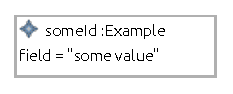
\includegraphics{images/05_library_of_transformations/03_instance_level_transformations/06_data_field_values/data_field_value.pdf}
        \caption{$Im_{DataField}$ with one object and string value ``some value''}
        \label{fig:library_of_transformations:instance_level_transformations:data_field_values:visualisation:ecore}
    \end{subfigure}
    \begin{subfigure}{0.45\textwidth}
        \centering
        \input{images/05_library_of_transformations/03_instance_level_transformations/06_data_field_values/data_field_as_edge_type_value.tikz}
        \caption{$IG_{DataField}$ with one node and string value ``some value''}
        \label{fig:library_of_transformations:instance_level_transformations:data_field_values:visualisation:groove}
    \end{subfigure}
    \caption{Visualisation of the transformation of field values from fields typed by data types}
    \label{fig:library_of_transformations:instance_level_transformations:data_field_values:visualisation}
\end{figure}

The previous sections have shown the instance level transformations of the introduction of all kinds of types and their instances. From this section onward, these types and their instances will be enriched by introducing fields. In this section, the instance level transformation belonging to the transformation of a data field is discussed. The type level transformation for data fields can be found in \cref{subsec:library_of_transformations:type_level_transformations:data_fields}. On the instance level, values for the data fields are introduced.

\begin{defin}[Instance model $Im_{DataField}$]
\label{defin:library_of_transformations:instance_level_transformations:data_field_values:imod_data_field}
Let $Im_{DataField}$ be an instance model typed by $Tm_{DataField}$ (\cref{defin:library_of_transformations:type_level_transformations:data_fields:tmod_data_field}). Define a set $objects$, which represent the objects that will get a value for the field introduced by $Tm_{DataField}$. Furthermore, define a function $obids$ which maps each of these objects to their corresponding identifier and a function $values$, which maps each of these objects to its value for the field introduced by $Tm_{DataField}$. $Im_{DataField}$ is defined as:
\begin{align*}
Object =\ &objects \\
\mathrm{ObjectClass} =\ & \begin{cases}
    (ob, classtype) & \mathrm{if }\ ob \in objects
\end{cases}\\
\mathrm{ObjectId} =\ & \begin{cases}
    (ob, obids(ob)) & \mathrm{if }\ ob \in objects
\end{cases}\\
\mathrm{FieldValue} =\ & \begin{cases}
    ((ob, (classtype, name)), values(ob)) & \mathrm{if }\ ob \in objects
\end{cases} \\
\mathrm{DefaultValue} =\ & \{\}
\end{align*}
\isabellelref{imod_data_field}{Ecore-GROOVE-Mapping-Library.DataFieldValue}
\end{defin}

\begin{thm}[Correctness of $Im_{DataField}$]
\label{defin:library_of_transformations:instance_level_transformations:data_field_values:imod_data_field_correct}
$Im_{DataField}$ (\cref{defin:library_of_transformations:instance_level_transformations:data_field_values:imod_data_field}) is a valid instance model in the sense of \cref{defin:formalisations:ecore_formalisation:instance_models:model_validity}.
\isabellelref{imod_data_field_correct}{Ecore-GROOVE-Mapping-Library.DataFieldValue}
\end{thm}

A visual representation of $Im_{DataField}$ with $objects = \{ob\}$ and $obids(ob) = someId$ can be seen in \cref{fig:library_of_transformations:instance_level_transformations:data_field_values:visualisation:ecore}. In this visualisation, the field value for $ob$ is defined as $values(ob) = \text{``some value''}$. Although this visualisation only shows one object, it is required to define a value for all objects that contain the field. Failing to do so would result in an invalid instance model after it is combined with another model, as the next definition will show. The correctness proof of $Im_{DataField}$ only is already quite involved, but not be included here for conciseness. It can be found as part of the validated Isabelle proofs.

In order to make composing transformation functions possible, $Im_{DataField}$ should be compatible with the instance model it is combined with.

\begin{thm}[Correctness of $\mathrm{combine}(Im, Im_{DataField})$]
\label{defin:library_of_transformations:instance_level_transformations:data_field_values:imod_data_field_combine_correct}
Assume an instance model $Im$ that is valid in the sense of \cref{defin:formalisations:ecore_formalisation:instance_models:model_validity}. Then $Im$ is compatible with $Im_{DataField}$ (in the sense of \cref{defin:transformation_framework:instance_models_and_instance_graphs:combining_instance_models:compatibility}) if:
\begin{itemize}
    \item All requirements of \cref{defin:library_of_transformations:type_level_transformations:data_fields:tmod_data_field_combine_correct} are met, to ensure the combination of the corresponding type models is valid;
    \item The class type on which the field is defined by $Tm_{DataField}$ may not be extended by another class type in the type model corresponding to $Im$;
    \item All of the objects in the set $objects$ must already be objects in $Im$;
    \item All objects typed by the class type on which the field is defined must occur in the set $objects$ and thus have a value in $Im_{DataField}$;
    \item For all of the objects in the set $objects$, the identifier set by $obids$ must be the same identifier as set by $Im$ for that object;
    \item For all objects in set $objects$, the value set by the $values$ function must be valid.
\end{itemize}
\isabellelref{imod_data_field_combine_correct}{Ecore-GROOVE-Mapping-Library.DataFieldValue}
\end{thm}

\begin{proof}
Use \cref{defin:transformation_framework:instance_models_and_instance_graphs:combining_instance_models:imod_combine_merge_correct}. It is possible to show that all assumptions hold. Now we have shown that $\mathrm{combine}(Im, Im_{DataField})$ is consistent in the sense of \cref{defin:formalisations:ecore_formalisation:instance_models:model_validity}.
\end{proof}

As explained earlier, $Im_{DataField}$ needs to introduce values for all objects that are typed by the class type on which the field is defined. This is enforced by the requirements of \cref{defin:library_of_transformations:instance_level_transformations:data_field_values:imod_data_field_combine_correct}. The proof is not included here for conciseness, but can be found as part of the validated proofs in Isabelle.

The definitions and theorems for introducing values for fields of data types within Ecore are now complete. 

\subsubsection{Encoding as edges and nodes}

In the type level transformation of data fields, data fields were encoded in GROOVE as edge types to an primitive type. On the instance level, this edge type will be used and edges will be created to give a value to each node type that has the field defined. The encoding corresponding to $Im_{DataField}$ can then be represented as $IG_{DataField}$, defined in the following definition:

\begin{defin}[Instance graph $IG_{DataField}$]
\label{defin:library_of_transformations:instance_level_transformations:data_field_values:ig_data_field_as_edge_type}
Let $IG_{DataField}$ be the instance graph typed by type graph $TG_{DataField}$ (\cref{defin:library_of_transformations:type_level_transformations:data_fields:tg_data_field_as_edge_type}). Reuse the set $objects$ from $Im_{DataField}$. Moreover, reuse the functions $obids$ and $values$ from $Im_{DataField}$.
The objects in the set $objects$ are converted to nodes in $Im_{DataField}$. For each of these objects, an edge of the encoded field is created. This edge targets a node that corresponds to the value set by $values$ for the corresponding object. Finally, the identity of the objects is defined using $obids$. $IG_{DataField}$ is defined as:
\begin{align*}
N =\ & objects \cup \{values(ob) \mid ob \in objects\} \\
E =\ & \big\{\big(ob, (\mathrm{ns\_\!to\_\!list}(classtype), \langle name \rangle, fieldtype), values(ob)\big) \mid ob \in objects \big\} \\
\mathrm{ident} =\ & \begin{cases}
    (obids(ob), ob) & \mathrm{if }\ ob \in objects
\end{cases}
\end{align*}
with
\begin{align*}
\mathrm{type}_n =\ & \begin{cases}
    (ob, \mathrm{ns\_\!to\_\!list}(classtype)) & \mathrm{if }\ ob \in objects
\end{cases}
\end{align*}
\isabellelref{ig_data_field_as_edge_type}{Ecore-GROOVE-Mapping-Library.DataFieldValue}
\end{defin}

\begin{thm}[Correctness of $IG_{DataField}$]
\label{defin:library_of_transformations:instance_level_transformations:data_field_values:ig_data_field_as_edge_type_correct}
$IG_{DataField}$ (\cref{defin:library_of_transformations:instance_level_transformations:data_field_values:ig_data_field_as_edge_type}) is a valid instance graph in the sense of \cref{defin:formalisations:groove_formalisation:instance_graphs:instance_graph_validity}.
\isabellelref{ig_data_field_as_edge_type_correct}{Ecore-GROOVE-Mapping-Library.DataFieldValue}
\end{thm}

A visual representation of $IG_{DataField}$ with $objects = \{ob\}$ and $obids(ob) = someId$ can be seen in \cref{fig:library_of_transformations:instance_level_transformations:data_field_values:visualisation:groove}. Like the previous visualisation, the field value for $ob$ is defined as $values(ob) = \text{``some value''}$. Although this visualisation only shows one node, it is required to define a value for all nodes typed by the node type corresponding to the field. Failing to do so would result in an invalid instance graph after it is combined with another graph, as the next definition will show. The correctness proof of $IG_{DataField}$ only is already quite involved, but not be included here for conciseness. It can be found as part of the validated Isabelle proofs.

In order to make composing transformation functions possible, $IG_{DataField}$ should be compatible with the instance graph it is combined with.

\begin{thm}[Correctness of $\mathrm{combine}(IG, IG_{DataField})$]
\label{defin:library_of_transformations:instance_level_transformations:data_field_values:ig_data_field_as_edge_type_combine_correct}
Assume an instance graph $IG$ that is valid in the sense of \cref{defin:formalisations:groove_formalisation:instance_graphs:instance_graph_validity}. Then $IG$ is compatible with $IG_{DataField}$ (in the sense of \cref{defin:transformation_framework:instance_models_and_instance_graphs:combining_instance_graphs:compatibility}) if:
\begin{itemize}
    \item All requirements of \cref{defin:library_of_transformations:type_level_transformations:data_fields:tg_data_field_as_edge_type_combine_correct} are met, to ensure the combination of the corresponding type graphs is valid;
    \item The node type on which the corresponding field is defined is not extended by other node types within the type graph corresponding to $IG$;
    \item All nodes in $IG$ that are typed by the node type on which the field is defined are also nodes in $IG_{DataField}$;
    \item For all nodes shared between $IG$ and $IG_{DataField}$, each node must have the same identifier in both $IG$ and $IG_{DataField}$;
    \item For all nodes for which the field is set, the $values$ function must define a valid value;
    \item If an primitive type has incoming or outgoing edge types in the type graph corresponding to $IG$, then the lower multiplicity of these edge types must be 0.
\end{itemize}
\isabellelref{ig_data_field_as_edge_type_combine_correct}{Ecore-GROOVE-Mapping-Library.DataFieldValue}
\end{thm}

\begin{proof}
Use \cref{defin:transformation_framework:instance_models_and_instance_graphs:combining_instance_graphs:ig_combine_merge_correct}. It is possible to show that all assumptions hold. Now we have shown that $\mathrm{combine}(IG, IG_{DataField})$ is valid in the sense of \cref{defin:formalisations:groove_formalisation:instance_graphs:instance_graph_validity}.
\end{proof}

Like the definition for the combination of instance models, the combination of instance graphs also requires the user to set a value for all nodes that are typed by the node type that corresponds to the field type. This is to keep the graph valid.

The next definitions define the transformation function from $Im_{DataField}$ to $IG_{DataField}$:

\begin{defin}[Transformation function $f_{DataField}$]
\label{defin:library_of_transformations:instance_level_transformations:data_field_values:imod_data_field_to_ig_data_field_as_edge_type}
The transformation function $f_{DataField}(Im)$ is defined as:
\begin{align*}
N =\ & Object_{Im} \cup \{values(ob) \mid ob \in Object_{Im}\}  \\
E =\ & \big\{\big(ob, (\mathrm{ns\_\!to\_\!list}(classtype), \langle name \rangle, fieldtype), values(ob)\big) \mid ob \in Object_{Im} \big\} \\
\mathrm{ident} =\ & \begin{cases}
    (obids(ob), ob) & \mathrm{if }\ ob \in Object_{Im}
\end{cases}
\end{align*}
with
\begin{align*}
\mathrm{type}_n =\ & \begin{cases}
    (ob, \mathrm{ns\_\!to\_\!list}(name)) & \mathrm{if }\ ob \in Object_{Im}
\end{cases}
\end{align*}
\isabellelref{imod_data_field_to_ig_data_field_as_edge_type}{Ecore-GROOVE-Mapping-Library.DataFieldValue}
\end{defin}

\begin{thm}[Correctness of $f_{DataField}$]
\label{defin:library_of_transformations:instance_level_transformations:data_field_values:imod_data_field_to_ig_data_field_as_edge_type_func}
$f_{DataField}(Im)$ (\cref{defin:library_of_transformations:instance_level_transformations:data_field_values:imod_data_field_to_ig_data_field_as_edge_type}) is a valid transformation function in the sense of \cref{defin:transformation_framework:instance_models_and_instance_graphs:combining_transformation_functions:transformation_function_instance_model_instance_graph} transforming $Im_{DataField}$ into $IG_{DataField}$.
\isabellelref{imod_data_field_to_ig_data_field_as_edge_type_func}{Ecore-GROOVE-Mapping-Library.DataFieldValue}
\end{thm}

The proof of the correctness of $f_{DataField}$ will not be included here. Instead, it can be found in the validated Isabelle theories.

Finally, to complete the transformation, the transformation function that transforms $IG_{DataField}$ into $Im_{DataField}$ is defined:

\begin{defin}[Transformation function $f'_{DataField}$]
\label{defin:library_of_transformations:instance_level_transformations:data_field_values:ig_data_field_as_edge_type_to_imod_data_field}
The transformation function $f'_{DataField}(IG)$ is defined as:
\begin{align*}
Object =\ &\{\mathrm{src}(e) \mid e \in E_{IG}\} \\
\mathrm{ObjectClass} =\ & \begin{cases}
    (ob, classtype) & \mathrm{if }\ ob \in \{\mathrm{src}(e) \mid e \in E_{IG}\}
\end{cases}\\
\mathrm{ObjectId} =\ & \begin{cases}
    (ob, obids(ob)) & \mathrm{if }\ ob \in \{\mathrm{src}(e) \mid e \in E_{IG}\}
\end{cases}\\
\mathrm{FieldValue} =\ & \begin{cases}
    ((ob, (classtype, name)), values(ob)) & \mathrm{if }\ ob \in \{\mathrm{src}(e) \mid e \in E_{IG}\}
\end{cases} \\
\mathrm{DefaultValue} =\ & \{\}
\end{align*}
\isabellelref{ig_data_field_as_edge_type_to_imod_data_field}{Ecore-GROOVE-Mapping-Library.DataFieldValue}
\end{defin}

\begin{thm}[Correctness of $f'_{DataField}$]
\label{defin:library_of_transformations:instance_level_transformations:data_field_values:ig_data_field_as_edge_type_to_tmod_class_func}
$f'_{DataField}(IG)$ (\cref{defin:library_of_transformations:instance_level_transformations:data_field_values:ig_data_field_as_edge_type_to_imod_data_field}) is a valid transformation function in the sense of \cref{defin:transformation_framework:instance_models_and_instance_graphs:combining_transformation_functions:transformation_function_instance_graph_instance_model} transforming $IG_{DataField}$ into $Im_{DataField}$.
\isabellelref{ig_data_field_as_edge_type_to_imod_data_field_func}{Ecore-GROOVE-Mapping-Library.DataFieldValue}
\end{thm}

Once more, the correctness proof is not included here but can be found in the validated Isabelle proofs of this thesis.
\subsection{Enumeration field values}
\label{subsec:library_of_transformations:instance_level_transformations:enum_field_values}

\begin{figure}
    \centering
    \begin{subfigure}{0.95\textwidth}
        \centering
        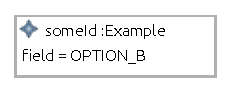
\includegraphics{images/05_library_of_transformations/03_instance_level_transformations/07_enum_field_values/enum_field_value.pdf}
        \caption{$Im_{EnumField}$ with one object and its field referencing enumeration option $OPTION\!\_B$}
        \label{fig:library_of_transformations:instance_level_transformations:enum_field_values:visualisation:ecore}
    \end{subfigure}
    \\
    \begin{subfigure}{0.95\textwidth}
        \centering
        \input{images/05_library_of_transformations/03_instance_level_transformations/07_enum_field_values/enum_as_node_types_field_as_edge_type_value.tikz}
        \caption{$IG_{EnumFieldNodes}$ with one node and and its edge referencing enumeration option $OPTION\!\_B$}
        \label{fig:library_of_transformations:instance_level_transformations:enum_field_values:visualisation:groove_nodes}
    \end{subfigure}
    \\
    \begin{subfigure}{0.95\textwidth}
        \centering
        \input{images/05_library_of_transformations/03_instance_level_transformations/07_enum_field_values/enum_as_flags_field_as_edge_type_value.tikz}
        \caption{$IG_{EnumFieldFlags}$ with one node and its edge referencing enumeration option $OPTION\!\_B$}
        \label{fig:library_of_transformations:instance_level_transformations:enum_field_values:visualisation:groove_flags}
    \end{subfigure}
    \caption{Visualisation of the transformation of field values from fields typed by enumeration types}
    \label{fig:library_of_transformations:instance_level_transformations:enum_field_values:visualisation}
\end{figure}

In this section, the instance level transformation belonging to the transformation of an enumeration field is discussed. The type level transformation for enumeration fields can be found in \cref{subsec:library_of_transformations:type_level_transformations:enum_fields}. On the instance level, values for the enumeration fields are introduced.

\begin{defin}[Instance model $Im_{EnumField}$]
\label{defin:library_of_transformations:instance_level_transformations:enum_field_values:imod_enum_field}
Let $Im_{EnumField}$ be an instance model typed by $Tm_{EnumField}$ (\cref{defin:library_of_transformations:type_level_transformations:enum_fields:tmod_enum_field}). Define a set $objects$, which represent the objects that will get a value for the field introduced by $Tm_{EnumField}$. Furthermore, define a function $obids$ which maps each of these objects to their corresponding identifier and a function $values$, which maps each of these objects to its value for the field introduced by $Tm_{EnumField}$. $Im_{EnumField}$ is defined as:
\begin{align*}
Object =\ &objects \\
\mathrm{ObjectClass} =\ & \begin{cases}
    (ob, classtype) & \mathrm{if }\ ob \in objects
\end{cases}\\
\mathrm{ObjectId} =\ & \begin{cases}
    (ob, obids(ob)) & \mathrm{if }\ ob \in objects
\end{cases}\\
\mathrm{FieldValue} =\ & \begin{cases}
    \Big((ob, (classtype, name)), \big[\type{enum}, (enumid, values(ob))\big]\Big) & \mathrm{if }\ ob \in objects
\end{cases} \\
\mathrm{DefaultValue} =\ & \{\}
\end{align*}
\isabellelref{imod_enum_field}{Ecore-GROOVE-Mapping-Library.EnumFieldValue}
\end{defin}

\begin{thm}[Correctness of $Im_{EnumField}$]
\label{defin:library_of_transformations:instance_level_transformations:enum_field_values:imod_enum_field_correct}
$Im_{EnumField}$ (\cref{defin:library_of_transformations:instance_level_transformations:enum_field_values:imod_enum_field}) is a valid instance model in the sense of \cref{defin:formalisations:ecore_formalisation:instance_models:model_validity}.
\isabellelref{imod_enum_field_correct}{Ecore-GROOVE-Mapping-Library.EnumFieldValue}
\end{thm}

A visual representation of $Im_{EnumField}$ with $objects = \{ob\}$ and $obids(ob) = someId$ can be seen in \cref{fig:library_of_transformations:instance_level_transformations:enum_field_values:visualisation:ecore}. In this visualisation, the field value for $ob$ is defined as $values(ob) = OPTION\!\_B$. Although this visualisation only shows one object, it is required to define a value for all objects that contain the field. Failing to do so would result in an invalid instance model after it is combined with another model, as the next definition will show. The correctness proof of $Im_{EnumField}$ only is quite involved, but not be included here for conciseness. It can be found as part of the validated Isabelle proofs.

In order to make composing transformation functions possible, $Im_{EnumField}$ should be compatible with the instance model it is combined with.

\begin{thm}[Correctness of $\mathrm{combine}(Im, Im_{EnumField})$]
\label{defin:library_of_transformations:instance_level_transformations:enum_field_values:imod_enum_field_combine_correct}
Assume an instance model $Im$ that is valid in the sense of \cref{defin:formalisations:ecore_formalisation:instance_models:model_validity}. Then $Im$ is compatible with $Im_{EnumField}$ (in the sense of \cref{defin:transformation_framework:instance_models_and_instance_graphs:combining_instance_models:compatibility}) if:
\begin{itemize}
    \item All requirements of \cref{defin:library_of_transformations:type_level_transformations:enum_fields:tmod_enum_field_combine_correct} are met, to ensure the combination of the corresponding type models is valid;
    \item The class type on which the field is defined by $Tm_{EnumField}$ may not be extended by another class type in the type model corresponding to $Im$;
    \item All of the objects in the set $objects$ must already be objects in $Im$;
    \item All objects typed by the class type on which the field is defined must occur in the set $objects$ and thus have a value in $Im_{EnumField}$;
    \item For all of the objects in the set $objects$, the identifier set by $obids$ must be the same identifier as set by $Im$ for that object;
    \item For all objects in set $objects$, the value set by the $values$ function must be valid.
\end{itemize}
\isabellelref{imod_enum_field_combine_correct}{Ecore-GROOVE-Mapping-Library.EnumFieldValue}
\end{thm}

\begin{proof}
Use \cref{defin:transformation_framework:instance_models_and_instance_graphs:combining_instance_models:imod_combine_merge_correct}. It is possible to show that all assumptions hold. Now we have shown that $\mathrm{combine}(Im, Im_{EnumField})$ is consistent in the sense of \cref{defin:formalisations:ecore_formalisation:instance_models:model_validity}.
\end{proof}

As explained earlier, $Im_{EnumField}$ needs to introduce values for all objects that are typed by the class type on which the field is defined. This is enforced by the requirements of \cref{defin:library_of_transformations:instance_level_transformations:enum_field_values:imod_enum_field_combine_correct}. The proof is not included here for conciseness, but can be found as part of the validated proofs in Isabelle.

The definitions and theorems for introducing values for fields of data types within Ecore are now complete. 

\subsubsection{Encoding as edges and nodes with a node type encoded enumeration type}

As discussed in \cref{subsec:library_of_transformations:type_level_transformations:enum_fields}, there are two different encodings for a field typed by an enumeration type. These correspond to the two different encodings of the enumeration type itself. On the instance level, these encodings also need to be distinguished. The first encoding of the values assumes that the enumeration is encoded using node types. The encoding corresponding to $Im_{EnumField}$ is then represented as $IG_{EnumFieldNodes}$, defined in the following definition:

\begin{defin}[Instance graph $IG_{EnumFieldNodes}$]
\label{defin:library_of_transformations:instance_level_transformations:enum_field_values:ig_enum_as_node_types_field_as_edge_type}
Let $IG_{EnumFieldNodes}$ be the instance graph typed by type graph $TG_{EnumFieldNodes}$ (\cref{defin:library_of_transformations:type_level_transformations:enum_fields:tg_enum_as_node_types_field_as_edge_type}). Reuse the set $objects$ from $Im_{EnumField}$. Moreover, reuse the functions $obids$ and $values$ from $Im_{EnumField}$. Furthermore, define $enumob$ to be the function that maps an enumeration value to an internal node identity. Similarly, define $enumids$ as the function that maps an enumeration value to its explicit node id.

Within $IG_{EnumFieldNodes}$, the objects in the set $objects$ are converted to nodes in $Im_{EnumField}$. For each of these objects, an edge of the encoded field is created. This edge targets a node that corresponds to the value set by $values$ for the corresponding object. Furthermore, the identity of the objects is defined using $obids$. Finally, ensure that the instances of the enumeration values exist and encode them in the same way as $IG_{EnumNodes}$ (\cref{defin:library_of_transformations:instance_level_transformations:enumeration_values:ig_enum_as_node_types}). $IG_{EnumFieldNodes}$ is defined as:
\begin{align*}
N =\ & objects \cup \{enumob(v) \mid v \in enumvalues \} \\
E =\ & \big\{\big(ob, (\mathrm{ns\_\!to\_\!list}(classtype), \langle name \rangle, \mathrm{ns\_\!to\_\!list}(enumid)), enumob(values(ob))\big) \mid ob \in objects \big\} \\
\mathrm{ident} =\ & \begin{cases}
    (obids(ob), ob) & \mathrm{if }\ ob \in objects\\
    (enumids(v), enumob(v)) & \mathrm{if }\ v \in enumvalues
\end{cases}
\end{align*}
with
\begin{align*}
\mathrm{type}_n =\ & \begin{cases}
    (ob, \mathrm{ns\_\!to\_\!list}(classtype)) & \mathrm{if }\ ob \in objects\\
    (enumob(v), \mathrm{ns\_\!to\_\!list}(enumid) \append \langle v \rangle) & \mathrm{if }\ v \in enumvalues
\end{cases}
\end{align*}
\isabellelref{ig_enum_as_node_types_field_as_edge_type}{Ecore-GROOVE-Mapping-Library.EnumFieldValue}
\end{defin}

\begin{thm}[Correctness of $IG_{EnumFieldNodes}$]
\label{defin:library_of_transformations:instance_level_transformations:enum_field_values:ig_enum_as_node_types_field_as_edge_type_correct}
$IG_{EnumFieldNodes}$ (\cref{defin:library_of_transformations:instance_level_transformations:enum_field_values:ig_enum_as_node_types_field_as_edge_type}) is a valid instance graph in the sense of \cref{defin:formalisations:groove_formalisation:instance_graphs:instance_graph_validity}.
\isabellelref{ig_enum_as_node_types_field_as_edge_type_correct}{Ecore-GROOVE-Mapping-Library.EnumFieldValue}
\end{thm}

A visual representation of $IG_{EnumFieldNodes}$ with $objects = \{ob\}$ and $obids(ob) = someId$ can be seen in \cref{fig:library_of_transformations:instance_level_transformations:enum_field_values:visualisation:groove_nodes}. Like the previous visualisation, the field value for $ob$ is defined as $values(ob) = OPTION\!\_B$. Although this visualisation only shows one node, it is required to define a value for all nodes that are typed by the node type corresponding to the field. Failing to do so would result in an invalid instance graph after it is combined with another graph, as the next definition will show. The correctness proof of $IG_{EnumFieldNodes}$ only is quite involved, but not be included here for conciseness. It can be found as part of the validated Isabelle proofs.

In order to make composing transformation functions possible, $IG_{EnumFieldNodes}$ should be compatible with the instance graph it is combined with.

\begin{thm}[Correctness of $\mathrm{combine}(IG, IG_{EnumFieldNodes})$]
\label{defin:library_of_transformations:instance_level_transformations:enum_field_values:ig_enum_as_node_types_field_as_edge_type_combine_correct}
Assume an instance graph $IG$ that is valid in the sense of \cref{defin:formalisations:groove_formalisation:instance_graphs:instance_graph_validity}. Then $IG$ is compatible with $IG_{EnumFieldNodes}$ (in the sense of \cref{defin:transformation_framework:instance_models_and_instance_graphs:combining_instance_graphs:compatibility}) if:
\begin{itemize}
    \item All requirements of \cref{defin:library_of_transformations:type_level_transformations:enum_fields:tg_enum_as_node_types_field_as_edge_type_combine_correct} are met, to ensure the combination of the corresponding type graphs is valid;
    \item The node type on which the corresponding field is defined is not extended by other node types within the type graph corresponding to $IG$;
    \item All nodes in $IG$ that are typed by the node type on which the field is defined are also nodes in $IG_{EnumFieldNodes}$;
    \item All nodes in $IG_{EnumFieldNodes}$ that encode the values of the corresponding enumeration type are also nodes in $IG$;
    \item For all nodes shared between $IG$ and $IG_{EnumFieldNodes}$, each node must have the same identifier in both $IG$ and $IG_{EnumFieldNodes}$;
    \item For all nodes for which the field is set, the $values$ function must define a valid value.
\end{itemize}
\isabellelref{ig_enum_as_node_types_field_as_edge_type_combine_correct}{Ecore-GROOVE-Mapping-Library.EnumFieldValue}
\end{thm}

\begin{proof}
Use \cref{defin:transformation_framework:instance_models_and_instance_graphs:combining_instance_graphs:ig_combine_merge_correct}. It is possible to show that all assumptions hold. Now we have shown that $\mathrm{combine}(IG, IG_{EnumFieldNodes})$ is valid in the sense of \cref{defin:formalisations:groove_formalisation:instance_graphs:instance_graph_validity}.
\end{proof}

Like the definition for the combination of instance models, the combination of instance graphs also requires the user to set a value for all nodes that are typed by the node type that corresponds to the field type. This is to keep the graph valid.

The next definitions define the transformation function from $Im_{EnumField}$ to $IG_{EnumFieldNodes}$:

\begin{defin}[Transformation function $f_{EnumFieldNodes}$]
\label{defin:library_of_transformations:instance_level_transformations:enum_field_values:imod_enum_field_to_ig_enum_as_node_types_field_as_edge_type}
The transformation function $f_{EnumFieldNodes}(Im)$ is defined as:
\begin{align*}
N =\ & Object_{Im} \cup \{enumob(ob) \mid v \in enumvalues\}  \\
E =\ & \big\{\big(ob, (\mathrm{ns\_\!to\_\!list}(classtype), \langle name \rangle, \mathrm{ns\_\!to\_\!list}(enumid)), enumob(values(ob))\big) \mid \\&ob \in Object_{Im} \big\} \\
\mathrm{ident} =\ & \begin{cases}
    (obids(ob), ob) & \mathrm{if }\ ob \in Object_{Im}\\
    (enumids(v), enumob(v)) & \mathrm{if }\ v \in enumvalues
\end{cases}
\end{align*}
with
\begin{align*}
\mathrm{type}_n =\ & \begin{cases}
    (ob, \mathrm{ns\_\!to\_\!list}(classtype)) & \mathrm{if }\ ob \in Object_{Im}\\
    (enumob(v), \mathrm{ns\_\!to\_\!list}(enumid) \append \langle v \rangle) & \mathrm{if }\ v \in enumvalues
\end{cases}
\end{align*}
\isabellelref{imod_enum_field_to_ig_enum_as_node_types_field_as_edge_type}{Ecore-GROOVE-Mapping-Library.EnumFieldValue}
\end{defin}

\begin{thm}[Correctness of $f_{EnumFieldNodes}$]
\label{defin:library_of_transformations:instance_level_transformations:enum_field_values:imod_enum_field_to_ig_enum_as_node_types_field_as_edge_type_func}
$f_{EnumFieldNodes}(Im)$ (\cref{defin:library_of_transformations:instance_level_transformations:enum_field_values:imod_enum_field_to_ig_enum_as_node_types_field_as_edge_type}) is a valid transformation function in the sense of \cref{defin:transformation_framework:instance_models_and_instance_graphs:combining_transformation_functions:transformation_function_instance_model_instance_graph} transforming $Im_{EnumField}$ into $IG_{EnumFieldNodes}$.
\isabellelref{imod_enum_field_to_ig_enum_as_node_types_field_as_edge_type_func}{Ecore-GROOVE-Mapping-Library.EnumFieldValue}
\end{thm}

The proof of the correctness of $f_{EnumFieldNodes}$ will not be included here. Instead, it can be found in the validated Isabelle theories.

Finally, to complete the transformation, the transformation function that transforms $IG_{EnumFieldNodes}$ into $Im_{EnumField}$ is defined:

\begin{defin}[Transformation function $f'_{EnumFieldNodes}$]
\label{defin:library_of_transformations:instance_level_transformations:enum_field_values:ig_enum_as_node_types_field_as_edge_type_to_imod_enum_field}
The transformation function $f'_{EnumFieldNodes}(IG)$ is defined as:
\begin{align*}
Object =\ &\{\mathrm{src}(e) \mid e \in E_{IG}\} \\
\mathrm{ObjectClass} =\ & \begin{cases}
    (ob, name) & \mathrm{if }\ ob \in \{\mathrm{src}(e) \mid e \in E_{IG}\}
\end{cases}\\
\mathrm{ObjectId} =\ & \begin{cases}
    (ob, obids(ob)) & \mathrm{if }\ ob \in \{\mathrm{src}(e) \mid e \in E_{IG}\}
\end{cases}\\
\mathrm{FieldValue} =\ & \begin{cases}
    \Big((ob, (classtype, name)), \big(\type{enum}, (enumid, values(ob))\big)\Big) & \mathrm{if }\ ob \in \{\mathrm{src}(e) \mid e \in E_{IG}\}
\end{cases} \\
\mathrm{DefaultValue} =\ & \{\}
\end{align*}
\isabellelref{ig_enum_as_node_types_field_as_edge_type_to_imod_enum_field}{Ecore-GROOVE-Mapping-Library.EnumFieldValue}
\end{defin}

\begin{thm}[Correctness of $f'_{EnumFieldNodes}$]
\label{defin:library_of_transformations:instance_level_transformations:enum_field_values:ig_enum_as_node_types_field_as_edge_type_to_tmod_class_func}
$f'_{EnumFieldNodes}(IG)$ (\cref{defin:library_of_transformations:instance_level_transformations:enum_field_values:ig_enum_as_node_types_field_as_edge_type_to_imod_enum_field}) is a valid transformation function in the sense of \cref{defin:transformation_framework:instance_models_and_instance_graphs:combining_transformation_functions:transformation_function_instance_graph_instance_model} transforming $IG_{EnumFieldNodes}$ into $Im_{EnumField}$.
\isabellelref{ig_enum_as_node_types_field_as_edge_type_to_imod_enum_field_func}{Ecore-GROOVE-Mapping-Library.EnumFieldValue}
\end{thm}

Once more, the correctness proof is not included here but can be found in the validated Isabelle proofs of this thesis.

\subsubsection{Encoding as edges and nodes with a flag encoded enumeration type}

The second possible encoding of the values assumes that the enumeration is encoded using flags. The encoding corresponding to $Im_{EnumField}$ is then represented as $IG_{EnumFieldFlags}$, defined in the following definition:

\begin{defin}[Instance graph $IG_{EnumFieldFlags}$]
\label{defin:library_of_transformations:instance_level_transformations:enum_field_values:ig_enum_as_flags_field_as_edge_type}
Let $IG_{EnumFieldFlags}$ be the instance graph typed by type graph $TG_{EnumFieldFlags}$ (\cref{defin:library_of_transformations:type_level_transformations:enum_fields:tg_enum_as_flags_field_as_edge_type}). Reuse the set $objects$ from $Im_{EnumField}$. Moreover, reuse the functions $obids$ and $values$ from $Im_{EnumField}$. Furthermore, define $enumob$ to be the function that maps an enumeration value to an internal node identity. Similarly, define $enumids$ as the function that maps an enumeration value to its explicit node id.

Within $IG_{EnumFieldFlags}$, the objects in the set $objects$ are converted to nodes in $Im_{EnumField}$. For each of these objects, an edge of the encoded field is created. This edge targets a node that corresponds to the value set by $values$ for the corresponding object. Furthermore, the identity of the objects is defined using $obids$. Finally, ensure that the instances of the enumeration values exist and encode them in the same way as $IG_{EnumFlags}$ (\cref{defin:library_of_transformations:instance_level_transformations:enumeration_values:ig_enum_as_flags}). $IG_{EnumFieldFlags}$ is defined as:
\begin{align*}
N =\ & objects \cup \{enumob(v) \mid v \in enumvalues \} \\
E =\ & \big\{\big(ob, (\mathrm{ns\_\!to\_\!list}(classtype), \langle name \rangle, \mathrm{ns\_\!to\_\!list}(enumid)), enumob(values(ob))\big) \mid ob \in objects \big\} \\
\mathrm{ident} =\ & \begin{cases}
    (obids(ob), ob) & \mathrm{if }\ ob \in objects\\
    (enumids(v), enumob(v)) & \mathrm{if }\ v \in enumvalues
\end{cases}
\end{align*}
with
\begin{align*}
\mathrm{type}_n =\ & \begin{cases}
    (ob, \mathrm{ns\_\!to\_\!list}(classtype)) & \mathrm{if }\ ob \in objects\\
    (enumob(v), \mathrm{ns\_\!to\_\!list}(enumid)) & \mathrm{if }\ v \in enumvalues
\end{cases}
\end{align*}
\isabellelref{ig_enum_as_flags_field_as_edge_type}{Ecore-GROOVE-Mapping-Library.EnumFieldValue}
\end{defin}

\begin{thm}[Correctness of $IG_{EnumFieldFlags}$]
\label{defin:library_of_transformations:instance_level_transformations:enum_field_values:ig_enum_as_flags_field_as_edge_type_correct}
$IG_{EnumFieldFlags}$ (\cref{defin:library_of_transformations:instance_level_transformations:enum_field_values:ig_enum_as_flags_field_as_edge_type}) is a valid instance graph in the sense of \cref{defin:formalisations:groove_formalisation:instance_graphs:instance_graph_validity}.
\isabellelref{ig_enum_as_flags_field_as_edge_type_correct}{Ecore-GROOVE-Mapping-Library.EnumFieldValue}
\end{thm}

A visual representation of $IG_{EnumFieldFlags}$ with $objects = \{ob\}$ and $obids(ob) = someId$ can be seen in \cref{fig:library_of_transformations:instance_level_transformations:enum_field_values:visualisation:groove_flags}. It does not differ much from the previous encoding, except that the values of the enumeration type are shown as flags on the nodes instead of using seperate types. The formal definition is therefore very similar, except for the definition of $\mathrm{type}_n$. Although this visualisation only shows one node, it is required to define a value for all nodes that are typed by the node type corresponding to the field. Failing to do so would, once more, result in an invalid instance graph after it is combined with another graph. The correctness proof of $IG_{EnumFieldFlags}$ only is quite involved, but not be included here for conciseness. It can be found as part of the validated Isabelle proofs.

In order to make composing transformation functions possible, $IG_{EnumFieldFlags}$ should be compatible with the instance graph it is combined with.

\begin{thm}[Correctness of $\mathrm{combine}(IG, IG_{EnumFieldFlags})$]
\label{defin:library_of_transformations:instance_level_transformations:enum_field_values:ig_enum_as_flags_field_as_edge_type_combine_correct}
Assume an instance graph $IG$ that is valid in the sense of \cref{defin:formalisations:groove_formalisation:instance_graphs:instance_graph_validity}. Then $IG$ is compatible with $IG_{EnumFieldFlags}$ (in the sense of \cref{defin:transformation_framework:instance_models_and_instance_graphs:combining_instance_graphs:compatibility}) if:
\begin{itemize}
    \item All requirements of \cref{defin:library_of_transformations:type_level_transformations:enum_fields:tg_enum_as_flags_field_as_edge_type_combine_correct} are met, to ensure the combination of the corresponding type graphs is valid;
    \item The node type on which the corresponding field is defined is not extended by other node types within the type graph corresponding to $IG$;
    \item All nodes in $IG$ that are typed by the node type on which the field is defined are also nodes in $IG_{EnumFieldFlags}$;
    \item All nodes in $IG_{EnumFieldFlags}$ that encode the values of the corresponding enumeration type are also nodes in $IG$;
    \item For all nodes shared between $IG$ and $IG_{EnumFieldFlags}$, each node must have the same identifier in both $IG$ and $IG_{EnumFieldFlags}$;
    \item For all nodes for which the field is set, the $values$ function must define a valid value.
\end{itemize}
\isabellelref{ig_enum_as_flags_field_as_edge_type_combine_correct}{Ecore-GROOVE-Mapping-Library.EnumFieldValue}
\end{thm}

\begin{proof}
Use \cref{defin:transformation_framework:instance_models_and_instance_graphs:combining_instance_graphs:ig_combine_merge_correct}. It is possible to show that all assumptions hold. Now we have shown that $\mathrm{combine}(IG, IG_{EnumFieldFlags})$ is valid in the sense of \cref{defin:formalisations:groove_formalisation:instance_graphs:instance_graph_validity}.
\end{proof}

The next definitions define the transformation function from $Im_{EnumField}$ to $IG_{EnumFieldFlags}$:

\begin{defin}[Transformation function $f_{EnumFieldFlags}$]
\label{defin:library_of_transformations:instance_level_transformations:enum_field_values:imod_enum_field_to_ig_enum_as_flags_field_as_edge_type}
The transformation function $f_{EnumFieldFlags}(Im)$ is defined as:
\begin{align*}
N =\ & Object_{Im} \cup \{enumob(ob) \mid v \in enumvalues\}  \\
E =\ & \big\{\big(ob, (\mathrm{ns\_\!to\_\!list}(classtype), \langle name \rangle, \mathrm{ns\_\!to\_\!list}(enumid)), enumob(values(ob))\big) \mid \\&ob \in Object_{Im} \big\} \\
\mathrm{ident} =\ & \begin{cases}
    (obids(ob), ob) & \mathrm{if }\ ob \in Object_{Im}\\
    (enumids(v), enumob(v)) & \mathrm{if }\ v \in enumvalues
\end{cases}
\end{align*}
with
\begin{align*}
\mathrm{type}_n =\ & \begin{cases}
    (ob, \mathrm{ns\_\!to\_\!list}(classtype)) & \mathrm{if }\ ob \in Object_{Im}\\
    (enumob(v), \mathrm{ns\_\!to\_\!list}(enumid)) & \mathrm{if }\ v \in enumvalues
\end{cases}
\end{align*}
\isabellelref{imod_enum_field_to_ig_enum_as_flags_field_as_edge_type}{Ecore-GROOVE-Mapping-Library.EnumFieldValue}
\end{defin}

\begin{thm}[Correctness of $f_{EnumFieldFlags}$]
\label{defin:library_of_transformations:instance_level_transformations:enum_field_values:imod_enum_field_to_ig_enum_as_flags_field_as_edge_type_func}
$f_{EnumFieldFlags}(Im)$ (\cref{defin:library_of_transformations:instance_level_transformations:enum_field_values:imod_enum_field_to_ig_enum_as_flags_field_as_edge_type}) is a valid transformation function in the sense of \cref{defin:transformation_framework:instance_models_and_instance_graphs:combining_transformation_functions:transformation_function_instance_model_instance_graph} transforming $Im_{EnumField}$ into $IG_{EnumFieldFlags}$.
\isabellelref{imod_enum_field_to_ig_enum_as_flags_field_as_edge_type_func}{Ecore-GROOVE-Mapping-Library.EnumFieldValue}
\end{thm}

The proof of the correctness of $f_{EnumFieldFlags}$ will not be included here. Instead, it can be found in the validated Isabelle theories.

Finally, to complete the transformation, the transformation function that transforms $IG_{EnumFieldFlags}$ into $Im_{EnumField}$ is defined:

\begin{defin}[Transformation function $f'_{EnumFieldFlags}$]
\label{defin:library_of_transformations:instance_level_transformations:enum_field_values:ig_enum_as_flags_field_as_edge_type_to_imod_enum_field}
The transformation function $f'_{EnumFieldFlags}(IG)$ is defined as:
\begin{align*}
Object =\ &\{\mathrm{src}(e) \mid e \in E_{IG}\} \\
\mathrm{ObjectClass} =\ & \begin{cases}
    (ob, classtype) & \mathrm{if }\ ob \in \{\mathrm{src}(e) \mid e \in E_{IG}\}
\end{cases}\\
\mathrm{ObjectId} =\ & \begin{cases}
    (ob, obids(ob)) & \mathrm{if }\ ob \in \{\mathrm{src}(e) \mid e \in E_{IG}\}
\end{cases}\\
\mathrm{FieldValue} =\ & \begin{cases}
    \Big((ob, (classtype, name)), \big[\type{enum}, (enumid, values(ob))\big]\Big) & \mathrm{if }\ ob \in \{\mathrm{src}(e) \mid e \in E_{IG}\}
\end{cases} \\
\mathrm{DefaultValue} =\ & \{\}
\end{align*}
\isabellelref{ig_enum_as_flags_field_as_edge_type_to_imod_enum_field}{Ecore-GROOVE-Mapping-Library.EnumFieldValue}
\end{defin}

\begin{thm}[Correctness of $f'_{EnumFieldFlags}$]
\label{defin:library_of_transformations:instance_level_transformations:enum_field_values:ig_enum_as_flags_field_as_edge_type_to_tmod_class_func}
$f'_{EnumFieldFlags}(IG)$ (\cref{defin:library_of_transformations:instance_level_transformations:enum_field_values:ig_enum_as_flags_field_as_edge_type_to_imod_enum_field}) is a valid transformation function in the sense of \cref{defin:transformation_framework:instance_models_and_instance_graphs:combining_transformation_functions:transformation_function_instance_graph_instance_model} transforming $IG_{EnumFieldFlags}$ into $Im_{EnumField}$.
\isabellelref{ig_enum_as_flags_field_as_edge_type_to_imod_enum_field_func}{Ecore-GROOVE-Mapping-Library.EnumFieldValue}
\end{thm}

Once more, the correctness proof is not included here but can be found in the validated Isabelle proofs of this thesis.
\subsection{Nullable class field values}
\label{subsec:library_of_transformations:instance_level_transformations:nullable_class_field_values}

\begin{figure}
    \centering
    \begin{subfigure}{0.95\textwidth}
        \centering
        \includegraphics{images/05_library_of_transformations/03_instance_level_transformations/08_nullable_class_field_values/nullable_class_field_value.pdf}
        \caption{$Im_{NullableClassField}$ with examples of different nodes with different values for $\type{field}$}
        \label{fig:library_of_transformations:instance_level_transformations:nullable_class_field_values:visualisation:ecore}
    \end{subfigure}
    \\
    \begin{subfigure}{0.95\textwidth}
        \centering
        \input{images/05_library_of_transformations/03_instance_level_transformations/08_nullable_class_field_values/nullable_class_field_as_edge_type_value.tikz}
        \caption{$IG_{NullableClassField}$ with examples of different nodes with different values for $\type{field}$}
        \label{fig:library_of_transformations:instance_level_transformations:nullable_class_field_values:visualisation:groove}
    \end{subfigure}
    \caption{Visualisation of the transformation of field values from fields typed by nullable class types}
    \label{fig:library_of_transformations:instance_level_transformations:nullable_class_field_values:visualisation}
\end{figure}

This section introduces the instance level transformation belonging to the transformation of a nullable class field. The type level transformation for nullable class fields can be found in \cref{subsec:library_of_transformations:type_level_transformations:nullable_class_fields}. On the instance level, values for these fields are introduced.

\begin{defin}[Instance model $Im_{NullableClassField}$]
\label{defin:library_of_transformations:instance_level_transformations:nullable_class_field_values:imod_nullable_class_field}
Let $Im_{NullableClassField}$ be an instance model typed by $Tm_{NullableClassField}$ (\cref{defin:library_of_transformations:type_level_transformations:nullable_class_fields:tmod_nullable_class_field}). Define disjoint sets $valobjects$ and $nilobjects$. The objects in $valobjects$ will get a proper class value for the field introduced by $Tm_{NullableClassField}$, while the objects in $nilobjects$ get a $\type{nil}$ value for the same field. Furthermore, define a function $obids$ which maps each of these objects to their corresponding identifier and a function $values$, which maps the objects in $valobjects$ to its value for the field introduced by $Tm_{NullableClassField}$. $Im_{NullableClassField}$ is defined as:
\begin{align*}
Object =\ &nilobjects \cup valobjects \cup \{ values(ob) \mid ob \in valobjects \} \\
\mathrm{ObjectClass} =\ & \begin{cases}
    (ob, classtype) & \mathrm{if }\ ob \in nilobjects \cup valobjects\\
    (ob, fieldtype) & \mathrm{if }\ ob \in \{ values(ob) \mid ob \in valobjects \}
\end{cases}\\
\mathrm{ObjectId} =\ & \begin{cases}
    (ob, obids(ob)) & \mathrm{if }\ ob \in objects
\end{cases}\\
\mathrm{FieldValue} =\ & \begin{cases}
    ((ob, (classtype, name)), \type{nil}) & \mathrm{if }\ ob \in nilobjects\\
    ((ob, (classtype, name)), [\type{obj}, values(ob)]) & \mathrm{if }\ ob \in valobjects
\end{cases} \\
\mathrm{DefaultValue} =\ & \{\}
\end{align*}
\isabellelref{imod_nullable_class_field}{Ecore-GROOVE-Mapping-Library.NullableClassFieldValue}
\end{defin}

\begin{thm}[Correctness of $Im_{NullableClassField}$]
\label{defin:library_of_transformations:instance_level_transformations:nullable_class_field_values:imod_nullable_class_field_correct}
$Im_{NullableClassField}$ (\cref{defin:library_of_transformations:instance_level_transformations:nullable_class_field_values:imod_nullable_class_field}) is a valid instance model in the sense of \cref{defin:formalisations:ecore_formalisation:instance_models:model_validity}.
\isabellelref{imod_nullable_class_field_correct}{Ecore-GROOVE-Mapping-Library.NullableClassFieldValue}
\end{thm}

A visual representation of $Im_{NullableClassField}$ with $valobjects = \{ob_a\}$ and $nilobjects = \{ob_b\}$ can be seen in \cref{fig:library_of_transformations:instance_level_transformations:nullable_class_field_values:visualisation:ecore}. In this visualisation, the field value for $ob_a$ is defined as $values(ob_a) = ob_x$. Furthermore, the value for $ob_b$ is $\type{nil}$, because it occurs within the set $nilobjects$. Like the previous transformations for field values, the value needs to be set for all objects that are typed by the class type corresponding to the field. Failing to do so would result in an invalid instance model after it is combined with another model, as the next definition will show. The correctness proof of $Im_{NullableClassField}$ only is already quite involved, but not be included here for conciseness. It can be found as part of the validated Isabelle proofs.

In order to make composing transformation functions possible, $Im_{NullableClassField}$ should be compatible with the instance model it is combined with.

\begin{thm}[Correctness of $\mathrm{combine}(Im, Im_{NullableClassField})$]
\label{defin:library_of_transformations:instance_level_transformations:nullable_class_field_values:imod_nullable_class_field_combine_correct}
Assume an instance model $Im$ that is valid in the sense of \cref{defin:formalisations:ecore_formalisation:instance_models:model_validity}. Then $Im$ is compatible with $Im_{NullableClassField}$ (in the sense of \cref{defin:transformation_framework:instance_models_and_instance_graphs:combining_instance_models:compatibility}) if:
\begin{itemize}
    \item All requirements of \cref{defin:library_of_transformations:type_level_transformations:nullable_class_fields:tmod_nullable_class_field_combine_correct} are met, to ensure the combination of the corresponding type models is valid;
    \item The class type on which the field is defined by $Tm_{NullableClassField}$ may not be extended by another class type in the type model corresponding to $Im$;
    \item All of the objects in the sets $nilobjects$ and $valobjects$ must already be objects in $Im$;
    \item All of the objects referenced by the objects in the set $valobjects$ must already be objects in $Im$;
    \item All objects typed by the class type on which the field is defined must occur in the set $nilobjects \cup valobjects$ and thus have a value in $Im_{NullableClassField}$;
    \item For all of the objects in the set $objects$, the identifier set by $obids$ must be the same identifier as set by $Im$ for that object;
    \item The sets $valobjects$ and $nilobjects$ must be disjoint, each object only gets a proper class value or a nil value, not both;
    \item For all objects in set $valobjects$, the value set by the $values$ function must be valid.
\end{itemize}
\isabellelref{imod_nullable_class_field_combine_correct}{Ecore-GROOVE-Mapping-Library.NullableClassFieldValue}
\end{thm}

\begin{proof}
Use \cref{defin:transformation_framework:instance_models_and_instance_graphs:combining_instance_models:imod_combine_merge_correct}. It is possible to show that all assumptions hold. Now we have shown that $\mathrm{combine}(Im, Im_{NullableClassField})$ is consistent in the sense of \cref{defin:formalisations:ecore_formalisation:instance_models:model_validity}.
\end{proof}

As explained earlier, $Im_{NullableClassField}$ needs to introduce values for all objects that are typed by the class type on which the field is defined. This is enforced by the requirements of \cref{defin:library_of_transformations:instance_level_transformations:nullable_class_field_values:imod_nullable_class_field_combine_correct}. The proof is not included here for conciseness, but can be found as part of the validated proofs in Isabelle.

The definitions and theorems for introducing values for fields of data types within Ecore are now complete. 

\subsubsection{Encoding as edges and nodes}

In the type level transformation of nullable class fields, nullable class fields were encoded in GROOVE as edge types to a corresponding encoded node type. On the instance level, this edge type will be used and edges will be created to give a value to each node type that has the field defined. The encoding corresponding to $Im_{NullableClassField}$ can then be represented as $IG_{NullableClassField}$, defined in the following definition:

\begin{defin}[Instance graph $IG_{NullableClassField}$]
\label{defin:library_of_transformations:instance_level_transformations:nullable_class_field_values:ig_nullable_class_field_as_edge_type}
Let $IG_{NullableClassField}$ be the instance graph typed by type graph $TG_{NullableClassField}$ (\cref{defin:library_of_transformations:type_level_transformations:nullable_class_fields:tg_nullable_class_field_as_edge_type}). Reuse the sets $nilobjects$ and $valobjects$ from $Im_{NullableClassField}$. Moreover, reuse the functions $obids$ and $values$ from $Im_{NullableClassField}$.

The objects in the sets $nilobjects$ and $valobjects$ are converted to nodes in $Im_{NullableClassField}$. For each of these objects, an edge of the encoded field is created. This edge targets a node that corresponds to the value set by $values$ for the corresponding object in $valobjects$. The outgoing multiplicity of the edge type created by $TG_{NullableClassField}$ is $0..1$, such that the objects in $nilobjects$ do not need to have this edge, representing the absence of a value. Finally, the identity of the objects is defined using $obids$. $IG_{NullableClassField}$ is defined as:
\begin{align*}
N =\ & nilobjects \cup valobjects \cup \{values(ob) \mid ob \in valobjects\} \\
E =\ & \big\{\big(ob, (\mathrm{ns\_\!to\_\!list}(classtype), \langle name \rangle, \mathrm{ns\_\!to\_\!list}(fieldtype)), values(ob)\big) \mid ob \in valobjects \big\} \\
\mathrm{ident} =\ & \begin{cases}
    (obids(ob), ob) & \mathrm{if }\ ob \in objects
\end{cases}
\end{align*}
with
\begin{align*}
\mathrm{type}_n =\ & \begin{cases}
    (ob, \mathrm{ns\_\!to\_\!list}(classtype)) & \mathrm{if }\ ob \in nilobjects \cup valobjects\\
    (ob, \mathrm{ns\_\!to\_\!list}(fieldtype)) & \mathrm{if }\ ob \in \{values(ob) \mid ob \in valobjects\}
\end{cases}
\end{align*}
\isabellelref{ig_nullable_class_field_as_edge_type}{Ecore-GROOVE-Mapping-Library.NullableClassFieldValue}
\end{defin}

\begin{thm}[Correctness of $IG_{NullableClassField}$]
\label{defin:library_of_transformations:instance_level_transformations:nullable_class_field_values:ig_nullable_class_field_as_edge_type_correct}
$IG_{NullableClassField}$ (\cref{defin:library_of_transformations:instance_level_transformations:nullable_class_field_values:ig_nullable_class_field_as_edge_type}) is a valid instance graph in the sense of \cref{defin:formalisations:groove_formalisation:instance_graphs:instance_graph_validity}.
\isabellelref{ig_nullable_class_field_as_edge_type_correct}{Ecore-GROOVE-Mapping-Library.NullableClassFieldValue}
\end{thm}

A visual representation of $IG_{NullableClassField}$ with $valobjects = \{ob_a\}$ and $nilobjects = \{ob_b\}$ can be seen in \cref{fig:library_of_transformations:instance_level_transformations:nullable_class_field_values:visualisation:groove}. Like the previous visualisation, the field value for $ob_a$ is defined as $values(ob_a) = ob_x$. Since $ob_b$ was in the set $nilobjects$, no edge has been created for this node. Like the previous field encodings, one needs to set the values for the field for all objects of the encoded class type at once. Failing to do so would result in an invalid instance graph after it is combined with another graph, as the next definition will show. The correctness proof of $IG_{NullableClassField}$ only is already quite involved, but not be included here for conciseness. It can be found as part of the validated Isabelle proofs.

In order to make composing transformation functions possible, $IG_{NullableClassField}$ should be compatible with the instance graph it is combined with.

\begin{thm}[Correctness of $\mathrm{combine}(IG, IG_{NullableClassField})$]
\label{defin:library_of_transformations:instance_level_transformations:nullable_class_field_values:ig_nullable_class_field_as_edge_type_combine_correct}
Assume an instance graph $IG$ that is valid in the sense of \cref{defin:formalisations:groove_formalisation:instance_graphs:instance_graph_validity}. Then $IG$ is compatible with $IG_{NullableClassField}$ (in the sense of \cref{defin:transformation_framework:instance_models_and_instance_graphs:combining_instance_graphs:compatibility}) if:
\begin{itemize}
    \item All requirements of \cref{defin:library_of_transformations:type_level_transformations:nullable_class_fields:tg_nullable_class_field_as_edge_type_combine_correct} are met, to ensure the combination of the corresponding type graphs is valid;
    \item The node type on which the corresponding field is defined is not extended by other node types within the type graph corresponding to $IG$;
    \item All nodes in $IG$ are also nodes in $IG_{NullableClassField}$;
    \item For all nodes shared between $IG$ and $IG_{NullableClassField}$, each node must have the same identifier in both $IG$ and $IG_{NullableClassField}$;
    \item The sets $valobjects$ and $nilobjects$ must be disjoint, each node gets either one edge to another node, or no edge at all;
    \item For all nodes for which the field is set, the $values$ function must define a valid value.
\end{itemize}
\isabellelref{ig_nullable_class_field_as_edge_type_combine_correct}{Ecore-GROOVE-Mapping-Library.NullableClassFieldValue}
\end{thm}

\begin{proof}
Use \cref{defin:transformation_framework:instance_models_and_instance_graphs:combining_instance_graphs:ig_combine_merge_correct}. It is possible to show that all assumptions hold. Now we have shown that $\mathrm{combine}(IG, IG_{NullableClassField})$ is valid in the sense of \cref{defin:formalisations:groove_formalisation:instance_graphs:instance_graph_validity}.
\end{proof}

The next definitions define the transformation function from $Im_{NullableClassField}$ to $IG_{NullableClassField}$:

\begin{defin}[Transformation function $f_{NullableClassField}$]
\label{defin:library_of_transformations:instance_level_transformations:nullable_class_field_values:imod_nullable_class_field_to_ig_nullable_class_field_as_edge_type}
The transformation function $f_{NullableClassField}(Im)$ is defined as:
\begin{align*}
N =\ & Object_{Im}  \\
E =\ & \big\{\big(ob, (\mathrm{ns\_\!to\_\!list}(classtype), \langle name \rangle, \mathrm{ns\_\!to\_\!list}(fieldtype)), values(ob)\big) \mid\\&ob \in Object_{Im} \land ob \in valobjects \big\} \\
\mathrm{ident} =\ & \begin{cases}
    (obids(ob), ob) & \mathrm{if }\ ob \in Object_{Im}
\end{cases}
\end{align*}
with
\begin{align*}
\mathrm{type}_n =\ & \begin{cases}
    (ob, \mathrm{ns\_\!to\_\!list}(name)) & \mathrm{if }\ ob \in Object_{Im} \land ob \in nilobjects \cup valobjects\\
    (ob, \mathrm{ns\_\!to\_\!list}(name)) & \mathrm{if }\ ob \in Object_{Im} \land ob \in \{values(ob) \mid ob \in valobjects\} 
\end{cases}
\end{align*}
\isabellelref{imod_nullable_class_field_to_ig_nullable_class_field_as_edge_type}{Ecore-GROOVE-Mapping-Library.NullableClassFieldValue}
\end{defin}

\begin{thm}[Correctness of $f_{NullableClassField}$]
\label{defin:library_of_transformations:instance_level_transformations:nullable_class_field_values:imod_nullable_class_field_to_ig_nullable_class_field_as_edge_type_func}
$f_{NullableClassField}(Im)$ (\cref{defin:library_of_transformations:instance_level_transformations:nullable_class_field_values:imod_nullable_class_field_to_ig_nullable_class_field_as_edge_type}) is a valid transformation function in the sense of \cref{defin:transformation_framework:instance_models_and_instance_graphs:combining_transformation_functions:transformation_function_instance_model_instance_graph} transforming $Im_{NullableClassField}$ into $IG_{NullableClassField}$.
\isabellelref{imod_nullable_class_field_to_ig_nullable_class_field_as_edge_type_func}{Ecore-GROOVE-Mapping-Library.NullableClassFieldValue}
\end{thm}

The proof of the correctness of $f_{NullableClassField}$ will not be included here. Instead, it can be found in the validated Isabelle theories.

Finally, to complete the transformation, the transformation function that transforms $IG_{NullableClassField}$ into $Im_{NullableClassField}$ is defined:

\begin{defin}[Transformation function $f'_{NullableClassField}$]
\label{defin:library_of_transformations:instance_level_transformations:nullable_class_field_values:ig_nullable_class_field_as_edge_type_to_imod_nullable_class_field}
The transformation function $f'_{NullableClassField}(IG)$ is defined as:
\begin{align*}
Object =\ &N_{IG} \\
\mathrm{ObjectClass} =\ & \begin{cases}
    (ob, classtype) & \mathrm{if }\ ob \in N_{IG} \land ob \in nilobjects \cup valobjects \\
    (ob, fieldtype) & \mathrm{if }\ ob \in N_{IG} \land ob \in \{values(ob) \mid ob \in valobjects\}
\end{cases}\\
\mathrm{ObjectId} =\ & \begin{cases}
    (ob, obids(ob)) & \mathrm{if }\ ob \in N_{IG}
\end{cases}\\
\mathrm{FieldValue} =\ & \begin{cases}
    ((ob, (classtype, name)), \type{nil}) & \mathrm{if }\ ob \in N_{IG} \land ob \in nilobjects\\
    ((ob, (classtype, name)), [\type{obj}, values(ob)]) & \mathrm{if }\ ob \in N_{IG} \land ob \in valobjects
\end{cases} \\
\mathrm{DefaultValue} =\ & \{\}
\end{align*}
\isabellelref{ig_nullable_class_field_as_edge_type_to_imod_nullable_class_field}{Ecore-GROOVE-Mapping-Library.NullableClassFieldValue}
\end{defin}

\begin{thm}[Correctness of $f'_{NullableClassField}$]
\label{defin:library_of_transformations:instance_level_transformations:nullable_class_field_values:ig_nullable_class_field_as_edge_type_to_tmod_class_func}
$f'_{NullableClassField}(IG)$ (\cref{defin:library_of_transformations:instance_level_transformations:nullable_class_field_values:ig_nullable_class_field_as_edge_type_to_imod_nullable_class_field}) is a valid transformation function in the sense of \cref{defin:transformation_framework:instance_models_and_instance_graphs:combining_transformation_functions:transformation_function_instance_graph_instance_model} transforming $IG_{NullableClassField}$ into $Im_{NullableClassField}$.
\isabellelref{ig_nullable_class_field_as_edge_type_to_imod_nullable_class_field_func}{Ecore-GROOVE-Mapping-Library.NullableClassFieldValue}
\end{thm}

Once more, the correctness proof is not included here but can be found in the validated Isabelle proofs of this thesis.
%\writingtask{Write about the proper class sequence field value transformation}
\subsection{Contained class set field values}
\label{subsec:library_of_transformations:instance_level_transformations:contained_class_set_field_values}

\begin{figure}
    \centering
    \begin{subfigure}{0.95\textwidth}
        \centering
        \includegraphics{images/05_library_of_transformations/03_instance_level_transformations/10_contained_class_set_field_values/contained_class_set_field_value.pdf}
        \caption{$Im_{ContainedClassSetField}$ with examples of different nodes with different values for $\type{field}$}
        \label{fig:library_of_transformations:instance_level_transformations:contained_class_set_field_values:visualisation:ecore}
    \end{subfigure}
    \\
    \begin{subfigure}{0.95\textwidth}
        \centering
        \input{images/05_library_of_transformations/03_instance_level_transformations/10_contained_class_set_field_values/contained_class_set_as_edge_type_value.tikz}
        \caption{$IG_{ContainedClassSetField}$ with examples of different nodes with different values for $\type{field}$}
        \label{fig:library_of_transformations:instance_level_transformations:contained_class_set_field_values:visualisation:groove}
    \end{subfigure}
    \caption{Visualisation of the transformation of field values from containment fields typed by a set of a proper class type}
    \label{fig:library_of_transformations:instance_level_transformations:contained_class_set_field_values:visualisation}
\end{figure}

This section introduces the instance level transformation belonging to the transformation of a containment field of a set of a proper class type. The type level transformation belonging to these fields can be found in \cref{subsec:library_of_transformations:type_level_transformations:contained_class_set_fields}. On the instance level, values for these fields are introduced.

\begin{defin}[Instance model $Im_{ContainedClassSetField}$]
\label{defin:library_of_transformations:instance_level_transformations:contained_class_set_field_values:imod_contained_class_set_field}
Let $Im_{ContainedClassSetField}$ be an instance model typed by $Tm_{ContainedClassSetField}$ (\cref{defin:library_of_transformations:type_level_transformations:contained_class_set_fields:tmod_contained_class_set_field}). Define a set $objects$, which represent the objects that will get a value for the field introduced by $Tm_{DataField}$. Furthermore, define a function $obids$ which maps each of these objects to their corresponding identifier and a function $values$, which maps each of these objects to its value for the field introduced by $Tm_{DataField}$. Please note that $values$ returns a set of objects, as the field allows for this. $Im_{DataField}$ is defined as:
\begin{align*}
Object =\ &objects \cup \bigg(\bigcup_{ob \in objects} values(ob)\bigg)\\
\mathrm{ObjectClass} =\ & \begin{cases}
    (ob, classtype) & \mathrm{if }\ ob \in objects\\
    (ob, containedtype) & \mathrm{if }\ ob \in \bigcup_{ob \in objects} values(ob)
\end{cases}\\
\mathrm{ObjectId} =\ & \begin{cases}
    (ob, obids(ob)) & \mathrm{if }\ ob \in objects
\end{cases}\\
\mathrm{FieldValue} =\ & \begin{cases}
    \Big((ob, (classtype, name)), \big[\type{setof}, \langle [\type{obj}, ob] \mid ob \in values(ob) \rangle\big]\Big) & \mathrm{if }\ ob \in objects
\end{cases} \\
\mathrm{DefaultValue} =\ & \{\}
\end{align*}
\isabellelref{imod_contained_class_set_field}{Ecore-GROOVE-Mapping-Library.ContainedClassSetFieldValue}
\end{defin}

\begin{thm}[Correctness of $Im_{ContainedClassSetField}$]
\label{defin:library_of_transformations:instance_level_transformations:contained_class_set_field_values:imod_contained_class_set_field_correct}
$Im_{ContainedClassSetField}$ (\cref{defin:library_of_transformations:instance_level_transformations:contained_class_set_field_values:imod_contained_class_set_field}) is a valid instance model in the sense of \cref{defin:formalisations:ecore_formalisation:instance_models:model_validity}.
\isabellelref{imod_contained_class_set_field_correct}{Ecore-GROOVE-Mapping-Library.ContainedClassSetFieldValue}
\end{thm}

A visual representation of $Im_{ContainedClassSetField}$ with $objects = \{ob_a, ob_b, ob_c\}$ can be seen in \cref{fig:library_of_transformations:instance_level_transformations:contained_class_set_field_values:visualisation:ecore}. This example is typed by $Tm_{ContainedClassSetField}$ in \cref{fig:library_of_transformations:type_level_transformations:contained_class_set_fields:visualisation:ecore}. In this visualisation, the field value for $ob_a$ is defined as $values(ob_a) = \{ob_x\}$. Furthermore, the value for $ob_b$ is $values(ob_a) = \{ob_y, ob_z\}$. Finally, the value for $ob_c$ is $values(ob_c) = \{\}$, which is allowed because the lower bound of the multiplicity is set 0 by the example. Like the previous transformations for field values, the value needs to be set for all objects that are typed by the class type corresponding to the field. Failing to do so would result in an invalid instance model after it is combined with another model, as the next definition will show. The correctness proof of $Im_{ContainedClassSetField}$ only is already quite involved, but not be included here for conciseness. It can be found as part of the validated Isabelle proofs.

In order to make composing transformation functions possible, $Im_{ContainedClassSetField}$ should be compatible with the instance model it is combined with.

\begin{thm}[Correctness of $\mathrm{combine}(Im, Im_{ContainedClassSetField})$]
\label{defin:library_of_transformations:instance_level_transformations:contained_class_set_field_values:imod_contained_class_set_field_combine_correct}
Assume an instance model $Im$ that is valid in the sense of \cref{defin:formalisations:ecore_formalisation:instance_models:model_validity}. Then $Im$ is compatible with $Im_{ContainedClassSetField}$ (in the sense of \cref{defin:transformation_framework:instance_models_and_instance_graphs:combining_instance_models:compatibility}) if:
\begin{itemize}
    \item All requirements of \cref{defin:library_of_transformations:type_level_transformations:contained_class_set_fields:tmod_contained_class_set_field_combine_correct} are met, to ensure the combination of the corresponding type models is valid;
    \item The class type on which the field is defined by $Tm_{ContainedClassSetField}$ may not be extended by another class type in the type model corresponding to $Im$;
    \item The contained type and the class type cannot be the same, e.g. $classtype \neq containedtype$.
    \item All of the objects in the set $objects$ must already be objects in $Im$;
    \item All of the referenced objects cannot be objects in $Im$, they are newly introduced by $Im_{ContainedClassSetField}$;
    \item All objects typed by the class type on which the field is defined must occur in the set $objects$ and thus have a value in $Im_{ContainedClassSetField}$;
    \item For all of the objects in the set $objects$, the identifier set by $obids$ must be the same identifier as set by $Im$ for that object;
    \item The object ids for the newly introduced objects must be unique with respect to each other and all other objects within $Im$;
    \item For all objects in set $valobjects$, the value set by the $values$ function must be valid and the amount of elements in each value must be within the multiplicity $mul$.
\end{itemize}
\isabellelref{imod_contained_class_set_field_combine_correct}{Ecore-GROOVE-Mapping-Library.ContainedClassSetFieldValue}
\end{thm}

\begin{proof}
Use \cref{defin:transformation_framework:instance_models_and_instance_graphs:combining_instance_models:imod_combine_merge_correct}. It is possible to show that all assumptions hold. Now we have shown that $\mathrm{combine}(Im, Im_{ContainedClassSetField})$ is consistent in the sense of \cref{defin:formalisations:ecore_formalisation:instance_models:model_validity}.
\end{proof}

Please note that all objects referenced by any objects via this field are newly created. They may not exist on the existing model. This is enforced to ensure that the containment relations of objects remain acyclic, which is needed to keep the instance model valid. The proof is not included here for conciseness, but can be found as part of the validated proofs in Isabelle.

The definitions and theorems for introducing values for fields of data types within Ecore are now complete. 

\subsubsection{Encoding as edges and nodes}

In the type level transformation of contained class set fields, a single containment edge type was introduced to encode the values for the containment field. On the instance level, the values for each object will be encoded using this edge type. The encoding corresponding to $Im_{ContainedClassSetField}$ can then be represented as $IG_{ContainedClassSetField}$, defined in the following definition:

\begin{defin}[Instance graph $IG_{ContainedClassSetField}$]
\label{defin:library_of_transformations:instance_level_transformations:contained_class_set_field_values:ig_contained_class_set_field_as_edge_type}
Let $IG_{ContainedClassSetField}$ be the instance graph typed by type graph $TG_{ContainedClassSetField}$ (\cref{defin:library_of_transformations:type_level_transformations:contained_class_set_fields:tg_contained_class_set_field_as_edge_type}). Reuse the set $objects$ from $Im_{ContainedClassSetField}$. Moreover, reuse the functions $obids$ and $values$ from $Im_{ContainedClassSetField}$.

The objects in the set $objects$ are converted to nodes in $Im_{ContainedClassSetField}$. For each of these objects, a edge is created for each referenced object within the value of that field. Each of these edges targets an node that encodes an object that was referenced by the value. Finally, the identity of the objects is defined using $obids$. $IG_{ContainedClassSetField}$ is defined as:
\begin{align*}
N =\ & objects \cup \bigg(\bigcup_{ob \in objects} values(ob)\bigg)\\
E =\ & \bigcup_{ob \in objects} \big\{\big(ob, (\mathrm{ns\_\!to\_\!list}(classtype), \langle name \rangle, \mathrm{ns\_\!to\_\!list}(containedtype)), v\big) \mid v \in values(ob) \big\} \\
\mathrm{ident} =\ & \begin{cases}
    (obids(ob), ob) & \mathrm{if }\ ob \in objects \cup \Big(\bigcup_{ob \in objects} values(ob)\Big)
\end{cases}
\end{align*}
with
\begin{align*}
\mathrm{type}_n =\ & \begin{cases}
    (ob, \mathrm{ns\_\!to\_\!list}(classtype)) & \mathrm{if }\ ob \in objects\\
    (v, \mathrm{ns\_\!to\_\!list}(containedtype)) & \mathrm{if }\ v \in \bigcup_{ob \in objects} values(ob)
\end{cases}
\end{align*}
\isabellelref{ig_contained_class_set_field_as_edge_type}{Ecore-GROOVE-Mapping-Library.ContainedClassSetFieldValue}
\end{defin}

\begin{thm}[Correctness of $IG_{ContainedClassSetField}$]
\label{defin:library_of_transformations:instance_level_transformations:contained_class_set_field_values:ig_contained_class_set_field_as_edge_type_correct}
$IG_{ContainedClassSetField}$ (\cref{defin:library_of_transformations:instance_level_transformations:contained_class_set_field_values:ig_contained_class_set_field_as_edge_type}) is a valid instance graph in the sense of \cref{defin:formalisations:groove_formalisation:instance_graphs:instance_graph_validity}.
\isabellelref{ig_contained_class_set_field_as_edge_type_correct}{Ecore-GROOVE-Mapping-Library.ContainedClassSetFieldValue}
\end{thm}

A visual representation of $IG_{ContainedClassSetField}$ with $objects = \{ob_a, ob_b, ob_c\}$ can be seen in \cref{fig:library_of_transformations:instance_level_transformations:contained_class_set_field_values:visualisation:groove}. This example is typed by $TG_{ContainedClassSetField}$ in \cref{fig:library_of_transformations:type_level_transformations:contained_class_set_fields:visualisation:groove}. In this visualisation, the field value for $ob_a$ is defined as $values(ob_a) = \{ob_x\}$. Furthermore, the value for $ob_b$ is $values(ob_a) = \{ob_y, ob_z\}$. Finally, the value for $ob_c$ is $values(ob_c) = \{\}$. Like the previous field encodings, one needs to set the values for the field for all objects of the encoded class type at once. Failing to do so would result in an invalid instance graph after it is combined with another graph, as the next definition will show. The correctness proof of $IG_{ContainedClassSetField}$ only is already quite involved, but not be included here for conciseness. It can be found as part of the validated Isabelle proofs.

In order to make composing transformation functions possible, $IG_{ContainedClassSetField}$ should be compatible with the instance graph it is combined with.

\begin{thm}[Correctness of $\mathrm{combine}(IG, IG_{ContainedClassSetField})$]
\label{defin:library_of_transformations:instance_level_transformations:contained_class_set_field_values:ig_contained_class_set_field_as_edge_type_combine_correct}
Assume an instance graph $IG$ that is valid in the sense of \cref{defin:formalisations:groove_formalisation:instance_graphs:instance_graph_validity}. Then $IG$ is compatible with $IG_{ContainedClassSetField}$ (in the sense of \cref{defin:transformation_framework:instance_models_and_instance_graphs:combining_instance_graphs:compatibility}) if:
\begin{itemize}
    \item All requirements of \cref{defin:library_of_transformations:type_level_transformations:contained_class_set_fields:tg_contained_class_set_field_as_edge_type_combine_correct} are met, to ensure the combination of the corresponding type graphs is valid;
    \item The node type on which the corresponding field is defined is not extended by other node types within the type graph corresponding to $IG$;
    \item The contained type and the class type cannot be the same, e.g. $classtype \neq containedtype$.
    \item All nodes in $objects$ are also nodes in $IG_{ContainedClassSetField}$;
    \item All nodes referenced by the nodes in $objects$ are not already nodes in $IG_{ContainedClassSetField}$, e.g. the nodes referenced by values are newly introduced;
    \item All nodes typed by the node type on which the field is defined must occur in the set $objects$ and thus have a value in $IG_{ContainedClassSetField}$;
    \item The object ids for the newly introduced objects must be unique with respect to each other and all other objects within $IG$;
    \item For all nodes shared between $IG$ and $IG_{ContainedClassSetField}$, each node must have the same identifier in both $IG$ and $IG_{ContainedClassSetField}$;
    \item For all nodes in set $objects$, the value set by the $values$ function must be valid and the amount of elements in each value must be within the multiplicity $mul$.
\end{itemize}
\isabellelref{ig_contained_class_set_field_as_edge_type_combine_correct}{Ecore-GROOVE-Mapping-Library.ContainedClassSetFieldValue}
\end{thm}

\begin{proof}
Use \cref{defin:transformation_framework:instance_models_and_instance_graphs:combining_instance_graphs:ig_combine_merge_correct}. It is possible to show that all assumptions hold. Now we have shown that $\mathrm{combine}(IG, IG_{ContainedClassSetField})$ is valid in the sense of \cref{defin:formalisations:groove_formalisation:instance_graphs:instance_graph_validity}.
\end{proof}

The next definitions define the transformation function from $Im_{ContainedClassSetField}$ to \\$IG_{ContainedClassSetField}$:

\begin{defin}[Transformation function $f_{ContainedClassSetField}$]
\label{defin:library_of_transformations:instance_level_transformations:contained_class_set_field_values:imod_contained_class_set_field_to_ig_contained_class_set_field_as_edge_type}
The transformation function $f_{ContainedClassSetField}(Im)$ is defined as:
\begin{align*}
N =\ & Object_{Im}\\
E =\ & \bigcup_{ob \in Object_{Im} \land ob \in objects} \big\{\big(ob, (\mathrm{ns\_\!to\_\!list}(classtype), \langle name \rangle, \mathrm{ns\_\!to\_\!list}(containedtype)), v\big) \mid\\&\qquad\qquad\qquad\qquad\qquad v \in values(ob) \big\} \\
\mathrm{ident} =\ & \begin{cases}
    (obids(ob), ob) & \mathrm{if }\ ob \in Object_{Im}
\end{cases}
\end{align*}
with
\begin{align*}
\mathrm{type}_n =\ & \begin{cases}
    (ob, \mathrm{ns\_\!to\_\!list}(classtype)) & \mathrm{if }\ ob \in Object_{Im} \land ob \in objects\\
    (v, \mathrm{ns\_\!to\_\!list}(containedtype)) & \mathrm{if }\ v \in \bigcup_{ob \in Object_{Im} \land ob \in objects} values(ob)
\end{cases}
\end{align*}
\isabellelref{imod_contained_class_set_field_to_ig_contained_class_set_field_as_edge_type}{Ecore-GROOVE-Mapping-Library.ContainedClassSetFieldValue}
\end{defin}

\begin{thm}[Correctness of $f_{ContainedClassSetField}$]
\label{defin:library_of_transformations:instance_level_transformations:contained_class_set_field_values:imod_contained_class_set_field_to_ig_contained_class_set_field_as_edge_type_func}
$f_{ContainedClassSetField}(Im)$ (\cref{defin:library_of_transformations:instance_level_transformations:contained_class_set_field_values:imod_contained_class_set_field_to_ig_contained_class_set_field_as_edge_type}) is a valid transformation function in the sense of \cref{defin:transformation_framework:instance_models_and_instance_graphs:combining_transformation_functions:transformation_function_instance_model_instance_graph} transforming $Im_{ContainedClassSetField}$ into $IG_{ContainedClassSetField}$.
\isabellelref{imod_contained_class_set_field_to_ig_contained_class_set_field_as_edge_type_func}{Ecore-GROOVE-Mapping-Library.ContainedClassSetFieldValue}
\end{thm}

The proof of the correctness of $f_{ContainedClassSetField}$ will not be included here. Instead, it can be found in the validated Isabelle theories.

Finally, to complete the transformation, the transformation function that transforms \\$IG_{ContainedClassSetField}$ into $Im_{ContainedClassSetField}$ is defined:

\begin{defin}[Transformation function $f'_{ContainedClassSetField}$]
\label{defin:library_of_transformations:instance_level_transformations:contained_class_set_field_values:ig_contained_class_set_field_as_edge_type_to_imod_contained_class_set_field}
The transformation function $f'_{ContainedClassSetField}(IG)$ is defined as:
\begin{align*}
Object =\ &N_{IG} \\
\mathrm{ObjectClass} =\ & \begin{cases}
    (ob, classtype) & \mathrm{if }\ ob \in N_{IG} \land ob \in objects\\
    (ob, containedtype) & \mathrm{if }\ ob \in N_{IG} \land ob \in \bigcup_{ob \in objects} values(ob)
\end{cases}\\
\mathrm{ObjectId} =\ & \begin{cases}
    (ob, obids(ob)) & \mathrm{if }\ ob \in N_{IG}
\end{cases}\\
\mathrm{FieldValue} =\ & \begin{cases}
    \Big((ob, (classtype, name)), \big[\type{setof}, \langle [\type{obj}, ob] \mid ob \in values(ob) \rangle\big]\Big) & \mathrm{if }\ ob \in N_{IG}\ \land\\&\quad ob \in objects
\end{cases} \\
\mathrm{DefaultValue} =\ & \{\}
\end{align*}
\isabellelref{ig_contained_class_set_field_as_edge_type_to_imod_contained_class_set_field}{Ecore-GROOVE-Mapping-Library.ContainedClassSetFieldValue}
\end{defin}

\begin{thm}[Correctness of $f'_{ContainedClassSetField}$]
\label{defin:library_of_transformations:instance_level_transformations:contained_class_set_field_values:ig_contained_class_set_field_as_edge_type_to_tmod_class_func}
$f'_{ContainedClassSetField}(IG)$ (\cref{defin:library_of_transformations:instance_level_transformations:contained_class_set_field_values:ig_contained_class_set_field_as_edge_type_to_imod_contained_class_set_field}) is a valid transformation function in the sense of \cref{defin:transformation_framework:instance_models_and_instance_graphs:combining_transformation_functions:transformation_function_instance_graph_instance_model} transforming $IG_{ContainedClassSetField}$ into $Im_{ContainedClassSetField}$.
\isabellelref{ig_contained_class_set_field_as_edge_type_to_imod_contained_class_set_field_func}{Ecore-GROOVE-Mapping-Library.ContainedClassSetFieldValue}
\end{thm}

Once more, the correctness proof is not included here but can be found in the validated Isabelle proofs of this thesis.
\chapter{Application}
\label{chapter:application}

This chapter will provide the necessary steps to apply the work presented in this thesis. So far, the thesis has introduced formalisations of Ecore and GROOVE, discussed in \cref{sec:formalisations:ecore_formalisation} and \cref{sec:formalisations:groove_formalisation} respectively. Furthermore, an transformation framework for reasoning about composable model transformations has been introduced as part of \cref{chapter:transformation_framework}. Finally, the previous chapter introduced some small transformations that represent the `building blocks' to use within the framework. In this chapter, the transformation framework is applied by building an example model from scratch, showing the necessary steps to apply the framework. Building the model will be done using the `building blocks' of the library of transformations. Furthermore, each of the steps is described formally using the formalisations presented earlier.

Contrary to the previous chapters, no distinction will be made between the type level and instance level. This distinction is unneeded because the different levels are ultimately tied to each other. When building an instance model or instance graph iteratively, a corresponding type model or type graph is build as well. Therefore, within this chapter, an instance model will be built. For each step in building the instance model, the corresponding step on the level of a type model will be discussed as well. Therefore, the steps for building both models are presented in a mixed fashion.

\section{The model}
\label{sec:application:the_model}

\begin{figure}[p]
    \centering
    \begin{subfigure}{0.98\textwidth}
        \centering
        \includegraphics{images/06_application/instance_model/step15.pdf}
        \caption{Instance model}
        \label{fig:application:the_model:final_ecore_model:instance_model}
    \end{subfigure}
    \\
    \begin{subfigure}{0.98\textwidth}
        \centering
        \includegraphics{images/06_application/type_model/step15.pdf}
        \caption{Type model}
        \label{fig:application:the_model:final_ecore_model:type_model}
    \end{subfigure}
    \caption{The final model of student housing}
    \label{fig:application:the_model:final_ecore_model}
\end{figure}

Throughout this chapter, the steps for building the same model are shown. The model that will be built is a model that represents student housing. A visualisation of the final Ecore model is included in \cref{fig:application:the_model:final_ecore_model}. Within the model, student houses are represented through the $.\type{House}$ type. A house can have 0 till 9 rooms, which are represented by the $.\type{Room}$ type. Each room can have one tenant, represented by the $.\type{Tenant}$. Possibly, the tenant can have another subtenant, which is modelled through the $\type{subtenant}$ relation.

Since many student houses have a name, this is reflected as such in the model. The $.\type{House}$ type has a $\type{string}$ attribute $\type{name}$ which represents the name of the house. Furthermore, some houses do have a common living room, while others do not. This is modelled through the $\type{boolean}$ attribute $\type{living\_\!room}$.

Each room within the house is identified by some identifier. Some houses number their rooms, and others use letters for the same purpose. The identifier of a room is reflected by the $\type{string}$ attribute $\type{room\_\!id}$. Furthermore, a room can either be small, medium or large. The size is used to determine the price of the room. This size of the room is represented using an enumeration type $.\type{RoomSize}$. Each room sets one size using the $\type{room\_\!size}$ attribute, which is typed by the $.\type{RoomSize}$ enumeration type.

For tenants, the model stores the name and the age through the $\type{string}$ attribute $\type{name}$ and $\type{int}$ attribute $\type{age}$ respectively. Furthermore, a tenant can be a regular tenant or a subtenant, which is represented using an another enumeration type $.\type{TenantType}$. Each tenant is either a regular tenant of a subtenant, which is modelled using the $\type{type}$ attribute, which is typed by the $.\type{TenantType}$ enumeration type.

In the next section, this model will be built in 15 steps. Furthermore, a corresponding GROOVE encoding will be built at the same time. At the end of the next section, the model of \cref{fig:application:the_model:final_ecore_model} is obtained, as well as the corresponding GROOVE encoding.
\section{Building the model}
\label{sec:application:building_the_model}

Within this section, the 15 steps are provided to build the model represented by \cref{fig:application:the_model:final_ecore_model}. For each of these 15 steps, the corresponding Ecore model and GROOVE graphs are shown.

Before the model is built, it is necessary to initialize the initial models. The initial models are empty and are used as a starting point. Each step will then add more elements to the model until the final model is obtained. Therefore, define the following models:

\begin{tabularx}{\textwidth}{|lX|}
\hline
\multicolumn{2}{|l|}{\textbf{Initial models}}\\
\hhline{|==|}
$Tm_0 = $ & $Tm_\epsilon$ (\cref{defin:transformation_framework:type_models_and_type_graphs:combining_type_models:empty_type_model}) \\
$Im_0 = $ & $Im_\epsilon$ (\cref{defin:transformation_framework:instance_models_and_instance_graphs:combining_instance_models:empty_instance_model})\\
\hline
$TG_0 = $ & $TG_\epsilon$ (\cref{defin:transformation_framework:type_models_and_type_graphs:combining_type_graphs:empty_type_graph})\\
$IG_0 = $ & $IG_\epsilon$ (\cref{defin:transformation_framework:instance_models_and_instance_graphs:combining_instance_graphs:empty_instance_graph})\\
\hline
$f_0(Im_0) = $ & $IG_\epsilon$ (\cref{defin:transformation_framework:instance_models_and_instance_graphs:combining_instance_graphs:empty_instance_graph})\\
$f'_0(IG_0) = $ & $Im_\epsilon$ (\cref{defin:transformation_framework:instance_models_and_instance_graphs:combining_instance_models:empty_instance_model})\\
\hline
\end{tabularx}

Essentially, every model is defined to be the empty model, and every graph is defined to be the empty graph. Furthermore, $f_0$ is the mapping function which projects $Im_0$ (and $Tm_0$) onto $IG_0$ (and $TG_0$). $f'_0$ is the inverse function which maps $IG_0$ (and $TG_0$) onto $Im_0$ (and $Tm_0$).

\subsection{Houses}
\label{subsec:application:building_the_model:houses}

The first step of building the model is to add a type. Without any types, nothing interesting can be produced. The first type will be the class type for houses. \cref{subsec:library_of_transformations:type_level_transformations:regular_classes} is used to introduce the class type, while on the instance level, \cref{subsec:library_of_transformations:instance_level_transformations:plain_objects} is used to introduce the house objects.

The $name$ of the new house type is $.\type{House}$. Furthermore, 2 house objects are introduced, $objects = \{TR, BHP\}$. Furthermore, we assume that the object identifiers are equal to the internal node id, so $fid(TR) = TR$ and $fid(BHP) = BHP$. The following model is obtained:

\LTXtable{\textwidth}{tex/06_application/02_building_the_model/tables/01_houses.tex}

\begin{figure}[p]
    \centering
    \begin{subfigure}{0.98\textwidth}
        \centering
        \includegraphics{images/06_application/instance_model/step01.pdf}
        \caption{Instance Model $Im_1$}
        \label{fig:application:building_the_model:houses:ecore:instance_model}
    \end{subfigure}
    \\
    \begin{subfigure}{0.98\textwidth}
        \centering
        \includegraphics{images/06_application/type_model/step01.pdf}
        \caption{Type Model $Tm_1$}
        \label{fig:application:building_the_model:houses:ecore:type_model}
    \end{subfigure}
    \caption{The Ecore model after step 1}
    \label{fig:application:building_the_model:houses:ecore}
\end{figure}

\begin{figure}[p]
    \centering
    \begin{subfigure}{0.98\textwidth}
        \centering
        \input{images/06_application/instance_graph/step01.tikz}
        \caption{Instance Graph $IG_1$}
        \label{fig:application:building_the_model:houses:groove:instance_graph}
    \end{subfigure}
    \\
    \begin{subfigure}{0.98\textwidth}
        \centering
        \input{images/06_application/type_graph/step01.tikz}
        \caption{Type Graph $TG_1$}
        \label{fig:application:building_the_model:houses:groove:type_graph}
    \end{subfigure}
    \caption{The GROOVE graphs after step 1}
    \label{fig:application:building_the_model:houses:groove}
\end{figure}

A visual representation of $Tm_1$ and $Im_1$ can be found in \cref{fig:application:building_the_model:houses:ecore}. Similarly, a visual representation of $TG_1$ and $IG_1$ can be found in \cref{fig:application:building_the_model:houses:groove}. Please note that because of the definitions of $f_1(Im_1)$ and $f'_1(IG_1)$, we have that $f_1(Im_1) = IG_1$ and $f'_1(IG_1) = Im_1$. Furthermore, $f_1(Im_1)$ and $f'_1(IG_1)$ are valid mapping functions themselves, such that they can be combined with another mapping function in the next step.

The models itself are not very special as of yet, but that is expected. Each step is only a small building block, and introducing a type is not very special.

\afterpage{\FloatBarrier}
\begin{longtable}{|lX|}
\hline
\multicolumn{2}{|l|}{\textbf{Models after step 2}}\\
\hhline{|==|}
\endhead
$Tm_2 = $ & $\mathrm{combine}(Tm_1, Tm_{Class}) =$ \newline
$\begin{aligned}
Class =\ & \{.\type{House}, .\type{Room}\} \\
Enum =\ & \{\} \\
UserDataType =\ & \{\} \\
Field =\ & \{\} \\
\mathrm{FieldSig} =\ & \{\} \\
EnumValue =\ & \{\} \\
Inh =\ & \{\} \\
Prop =\ & \{\} \\
Constant =\ & \{\} \\
\mathrm{ConstType} =\ & \{\}
\end{aligned}$
\\
$Im_2 = $ & $\mathrm{combine}(Tm_1, Im_{Class}) =$ \newline
$\begin{aligned}
Object =\ &\{TR, BHP\} \\
\mathrm{ObjectClass}(ob) =\ & \{(TR, .\type{House}), (BHP, .\type{House})\}\\
\mathrm{ObjectId} =\ & \{(TR, TR), (BHP, BHP)\}\\
\mathrm{FieldValue} =\ & \{\} \\
\mathrm{DefaultValue} =\ & \{\}
\end{aligned}$
\\
\hline
$TG_2 = $ & $\mathrm{combine}(TG_1, TG_{Class}) =$ \newline
$\begin{aligned}
NT =\ & \{\langle \type{House} \rangle, \langle \type{Room} \rangle\} \\
ET =\ & \{\} \\
\!\!\sqsubseteq\ =\ & \big\{
\big(\langle \type{House} \rangle, \langle \type{House} \rangle \big),
\big(\langle \type{Room} \rangle, \langle \type{Room} \rangle \big)
\big\} \\
abs =\ & \{\} \\
\mathrm{mult} =\ & \{\} \\
contains =\ & \{\}
\end{aligned}$
\\
$IG_2 = $ & $\mathrm{combine}(TG_1, IG_{Class}) =$ \newline
$\begin{aligned}
N =\ & \{TR, BHP\} \\
E =\ & \{\} \\
\mathrm{ident} =\ & \{(TR, TR), (BHP, BHP)\} \\
\mathrm{type}_n =\ & \{(TR, \langle \type{House} \rangle), (BHP, \langle \type{House} \rangle)\}
\end{aligned}$
\\
\hline
$f_2(Im_2) = $ & $f_1(Im_1) \sqcup f_{Class}(Im_{Class})$ (\cref{defin:transformation_framework:instance_models_and_instance_graphs:combining_transformation_functions:combination_transformation_function_instance_model_instance_graph})\\
$f'_2(IG_2) = $ & $f'_1(IG_1) \sqcup f'_{Class}(IG_{Class})$ (\cref{defin:transformation_framework:instance_models_and_instance_graphs:combining_transformation_functions:combination_transformation_function_instance_graph_instance_model})\\
\hline
\end{longtable}
\begin{longtable}{|lX|}
\hline
\multicolumn{2}{|l|}{\textbf{Models after step 3}}\\
\hhline{|==|}
\endhead
$Tm_3 = $ & $\mathrm{combine}(Tm_2, Tm_{DataField}) =$ \newline
$\begin{aligned}
Class =\ & \{.\type{House}, .\type{Room}\} \\
Enum =\ & \{\} \\
UserDataType =\ & \{\} \\
Field =\ & \{(.\type{House}, \type{name})\} \\
\mathrm{FieldSig} =\ & \big\{\big((.\type{House}, \type{name}), (\type{string}, 1..1)\big)\big\} \\
EnumValue =\ & \{\} \\
Inh =\ & \{\} \\
Prop =\ & \{\} \\
Constant =\ & \{\} \\
\mathrm{ConstType} =\ & \{\}
\end{aligned}$
\\
$Im_3 = $ & $\mathrm{combine}(Tm_2, Im_{DataField}) =$ \newline
$\begin{aligned}
Object =\ &\{TR, BHP\} \\
\mathrm{ObjectClass}(ob) =\ & \{(TR, .\type{House}), (BHP, .\type{House})\}\\
\mathrm{ObjectId} =\ & \{(TR, TR), (BHP, BHP)\}\\
\mathrm{FieldValue} =\ & \Big\{
\Big(\big(TR, (.\type{House}, \type{name})\big), \big[\type{string}, \text{``TwoRem''}\big]\Big),\\&
\Big(\big(BHP, (.\type{House}, \type{name})\big), \big[\type{string}, \text{``B.H. Paleis''}\big]\Big)
\Big\} \\
\mathrm{DefaultValue} =\ & \{\}
\end{aligned}$
\\
\hline
$TG_3 = $ & $\mathrm{combine}(TG_2, TG_{DataField}) =$ \newline
$\begin{aligned}
NT =\ & \{\langle \type{House} \rangle, \langle \type{Room} \rangle, \type{string}\} \\
ET =\ & \big\{
\big(\langle \type{House} \rangle, \langle \type{name} \rangle, \type{string} \big)
\big\} \\
\!\!\sqsubseteq\ =\ & \big\{
\big(\langle \type{House} \rangle, \langle \type{House} \rangle \big),
\big(\langle \type{Room} \rangle, \langle \type{Room} \rangle \big),
\big(\type{string}, \type{string} \big)
\big\} \\
abs =\ & \{\} \\
\mathrm{mult} =\ & \Big\{
\Big(\big(\langle \type{House} \rangle, \langle \type{name} \rangle, \type{string} \big), \big(0..\mstar, 1..1\big) \Big)
\Big\} \\
contains =\ & \{\}
\end{aligned}$
\\
$IG_3 = $ & $\mathrm{combine}(TG_2, IG_{DataField}) =$ \newline
$\begin{aligned}
N =\ & \{TR, BHP, \text{``TwoRem''}, \text{``B.H. Paleis''}\} \\
E =\ & \Big\{
\Big(TR, \big(\langle \type{House} \rangle, \langle \type{name} \rangle, \type{string} \big), \text{``TwoRem''} \Big),\\&
\Big(BHP, \big(\langle \type{House} \rangle, \langle \type{name} \rangle, \type{string} \big), \text{``B.H. Paleis''} \Big)
\Big\} \\
\mathrm{ident} =\ & \{(TR, TR), (BHP, BHP)\} \\
\mathrm{type}_n =\ & \{
(TR, \langle \type{House} \rangle), 
(BHP, \langle \type{House} \rangle),
(\text{``TwoRem''}, \type{string}),
(\text{``B.H. Paleis''}, \type{string})
\}
\end{aligned}$
\\
\hline
$f_3(Im_3) = $ & $f_2(Im_2) \sqcup f_{DataField}(Im_{DataField})$ (\cref{defin:transformation_framework:instance_models_and_instance_graphs:combining_transformation_functions:combination_transformation_function_instance_model_instance_graph})\\
$f'_3(IG_3) = $ & $f'_2(IG_2) \sqcup f'_{DataField}(IG_{DataField})$ (\cref{defin:transformation_framework:instance_models_and_instance_graphs:combining_transformation_functions:combination_transformation_function_instance_graph_instance_model})\\
\hline
\end{longtable}
\subsection{Rooms}
\label{subsec:application:building_the_model:rooms}

In the fourth step, the room objects will be introduced as part of the introduction of the rooms containment relation. This step introduces the $\type{rooms}$ relation on the $.\type{House}$ class, including its values. \cref{subsec:library_of_transformations:type_level_transformations:contained_class_set_fields} is used to introduce the field, while on the instance level, \cref{subsec:library_of_transformations:instance_level_transformations:contained_class_set_field_values} is used to introduce the values.

The $classtype$ of the new field is $.\type{House}$, as the field will be defined for houses. The $name$ of the new field is $\type{rooms}$ and the $containedtype$ is $.\type{Room}$. The set of objects of which the value is set is equal to all house objects, so $objects = \{TR, BHP\}$. The function for $obids$ returns the existing identifier of each of these objects. The multiplicity is set to $0..9$ for the new field, and the $values$ function is defined as follows:
\begin{equation*}
    values = \big\{\big(TR, \{TRRoom1, TRRoom2\}\big), \big(BHP, \{BHPRoomA, BHPRoomB, BHPRoomC\}\big)\big\}
\end{equation*}

Please note that the referenced objects are all new. For these new objects $obids$ returns as identifier the internal node label, just as was done for the houses. The following model is obtained:

\LTXtable{\textwidth}{tex/06_application/02_building_the_model/tables/04_rooms.tex}

\begin{figure}[p]
    \centering
    \begin{subfigure}{0.98\textwidth}
        \centering
        \includegraphics{images/06_application/instance_model/step04.pdf}
        \caption{Instance Model $Im_4$}
        \label{fig:application:building_the_model:rooms:ecore:instance_model}
    \end{subfigure}
    \\
    \begin{subfigure}{0.98\textwidth}
        \centering
        \includegraphics{images/06_application/type_model/step04.pdf}
        \caption{Type Model $Tm_4$}
        \label{fig:application:building_the_model:rooms:ecore:type_model}
    \end{subfigure}
    \caption{The Ecore model after step 4}
    \label{fig:application:building_the_model:rooms:ecore}
\end{figure}

\begin{figure}[p]
    \centering
    \begin{subfigure}{0.98\textwidth}
        \centering
        \input{images/06_application/instance_graph/step04.tikz}
        \caption{Instance Graph $IG_4$}
        \label{fig:application:building_the_model:rooms:groove:instance_graph}
    \end{subfigure}
    \\
    \begin{subfigure}{0.98\textwidth}
        \centering
        \input{images/06_application/type_graph/step04.tikz}
        \caption{Type Graph $TG_4$}
        \label{fig:application:building_the_model:rooms:groove:type_graph}
    \end{subfigure}
    \caption{The GROOVE graphs after step 4}
    \label{fig:application:building_the_model:rooms:groove}
\end{figure}

A visual representation of $Tm_4$ and $Im_4$ can be found in \cref{fig:application:building_the_model:rooms:ecore}. Similarly, a visual representation of $TG_4$ and $IG_4$ can be found in \cref{fig:application:building_the_model:rooms:groove}. Please note that because of the definitions of $f_4(Im_4)$ and $f'_4(IG_4)$, we have that $f_4(Im_4) = IG_4$ and $f'_4(IG_4) = Im_4$. Furthermore, $f_4(Im_4)$ and $f'_4(IG_4)$ are valid mapping functions themselves, such that they can be combined with another mapping function in the next step.

The introduction of the room objects makes that the model represents something. A house has rooms that it contains, and each house has a different set of rooms. Still, there is room to enlarge the model more, such that more details are included.

\afterpage{\FloatBarrier}
\subsection{Room identifiers}
\label{sec:application:building_the_model:room_identifiers}

In the fifth step, the room identifiers are introduced by introducing another $\type{string}$ field. This step introduces gives each room a size, or in model terms, the $\type{room\_size}$ attribute on the $.\type{Room}$ class is introduced, including its values. \cref{subsec:library_of_transformations:type_level_transformations:enum_fields} is used to introduce the field on the type level, while on the instance level, \cref{subsec:library_of_transformations:instance_level_transformations:enum_field_values} is used to introduce the values.

The $classtype$ of the new field is $.\type{Room}$, as the field will be defined for rooms. The $name$ of the new field is $\type{room\_\!id}$ and the $fieldtype$ is $.\type{string}$. The set of objects of which the value is set is equal to all room objects, so $objects = \{TRRoom1, TRRoom2, BHPRoomA, BHPRoomB, BHPRoomC\}$. The function for $obids$ returns the existing identifier of each of these objects. The $values$ function is defined as follows:
\begin{align*}
    values = \{&(TRRoom1, \text{``1''}), (TRRoom2, \text{``2''}), (BHPRoomA, \text{``A''}), \\&(BHPRoomB, \text{``B''}), (BHPRoomC, \text{``C''})\}
\end{align*}

The following model is obtained:

\LTXtable{\textwidth}{tex/06_application/02_building_the_model/tables/05_room_identifiers.tex}

\begin{figure}[p]
    \centering
    \begin{subfigure}{0.98\textwidth}
        \centering
        \includegraphics{images/06_application/instance_model/step05.pdf}
        \caption{Instance Model $Im_5$}
        \label{fig:application:building_the_model:room_identifiers:ecore:instance_model}
    \end{subfigure}
    \\
    \begin{subfigure}{0.98\textwidth}
        \centering
        \includegraphics{images/06_application/type_model/step05.pdf}
        \caption{Type Model $Tm_5$}
        \label{fig:application:building_the_model:room_identifiers:ecore:type_model}
    \end{subfigure}
    \caption{The Ecore model after step 5}
    \label{fig:application:building_the_model:room_identifiers:ecore}
\end{figure}

\begin{figure}[p]
    \centering
    \begin{subfigure}{0.98\textwidth}
        \centering
        \input{images/06_application/instance_graph/step05.tikz}
        \caption{Instance Graph $IG_5$}
        \label{fig:application:building_the_model:room_identifiers:groove:instance_graph}
    \end{subfigure}
    \\
    \begin{subfigure}{0.98\textwidth}
        \centering
        \input{images/06_application/type_graph/step05.tikz}
        \caption{Type Graph $TG_5$}
        \label{fig:application:building_the_model:room_identifiers:groove:type_graph}
    \end{subfigure}
    \caption{The GROOVE graphs after step 5}
    \label{fig:application:building_the_model:room_identifiers:groove}
\end{figure}

A visual representation of $Tm_5$ and $Im_5$ can be found in \cref{fig:application:building_the_model:room_identifiers:ecore}. Similarly, a visual representation of $TG_5$ and $IG_5$ can be found in \cref{fig:application:building_the_model:room_identifiers:groove}. Please note that because of the definitions of $f_5(Im_5)$ and $f'_5(IG_5)$, we have that $f_5(Im_5) = IG_5$ and $f'_5(IG_5) = Im_5$. Furthermore, $f_5(Im_5)$ and $f'_5(IG_5)$ are valid mapping functions themselves, such that they can be combined with another mapping function in the next step.

The visualisation unveils no surprising details. A string field was already added earlier to the house objects and introducing such a field on the room only shows that it is indeed possible to introduce fields on contained objects.

\afterpage{\FloatBarrier}
\begin{longtable}{|lX|}
\hline
\multicolumn{2}{|l|}{\textbf{Models after step 6}}\\
\hhline{|==|}
\endhead
$Tm_6 = $ & $\mathrm{combine}(Tm_5, Tm_{Enum}) =$ \newline
$\begin{aligned}
Class =\ & \{.\type{House}, .\type{Room}\} \\
Enum =\ & \{.\type{RoomSize}\} \\
UserDataType =\ & \{\} \\
Field =\ & \{(.\type{House}, \type{name}), (.\type{House}, \type{rooms}), (.\type{Room}, \type{room\_\!id})\} \\
\mathrm{FieldSig} =\ & \big\{
\big((.\type{House}, \type{name}), (\type{string}, 1..1)\big),\\&
\big((.\type{House}, \type{rooms}), ([\type{setof}, !.\type{Room}], 0..9)\big),\\&
\big((.\type{Room}, \type{room\_\!id}), (\type{string}, 1..1)\big)
\big\} \\
EnumValue =\ & \{(.\type{RoomSize}, \type{SMALL}), (.\type{RoomSize}, \type{MEDIUM}), (.\type{RoomSize}, \type{LARGE})\} \\
Inh =\ & \{\} \\
Prop =\ & \big\{\big(\type{containment}, (.\type{House}, \type{rooms})\big)\big\} \\
Constant =\ & \{\} \\
\mathrm{ConstType} =\ & \{\}
\end{aligned}$
\\
$Im_6 = $ & $\mathrm{combine}(Tm_5, Im_{Enum}) =$ \newline
$\begin{aligned}
Object =\ &\{TR, BHP, TRRoom1, TRRoom2, BHPRoomA, BHPRoomB, \\& BHPRoomC\} \\
\mathrm{ObjectClass}(ob) =\ & \{(TR, .\type{House}), (BHP, .\type{House}),
(TRRoom1, .\type{Room}),\\& (TRRoom2, .\type{Room}), (BHPRoomA, .\type{Room}), (BHPRoomB, .\type{Room}),\\& (BHPRoomC, .\type{Room})\}\\
\mathrm{ObjectId} =\ & \{(TR, TR), (BHP, BHP), (TRRoom1, TRRoom1),\\& (TRRoom2, TRRoom2), (BHPRoomA, BHPRoomA),\\& (BHPRoomB, BHPRoomB), (BHPRoomC, BHPRoomC)\}\\
\mathrm{FieldValue} =\ & \Big\{
\Big(\big(TR, (.\type{House}, \type{name})\big), \big[\type{string}, \text{``TwoRem''}\big]\Big),\\&
\Big(\big(BHP, (.\type{House}, \type{name})\big), \big[\type{string}, \text{``B.H. Paleis''}\big]\Big),\\&
\Big(\big(TR, (.\type{House}, \type{rooms})\big), \big[\type{setof}, \big\langle [\type{obj}, TRRoom1], \\&\qquad [\type{obj}, TRRoom2] \big\rangle \big]\Big),\\&
\Big(\big(BHP, (.\type{House}, \type{rooms})\big) \big[\type{setof}, \big\langle [\type{obj},  BHPRoomA], \\&\qquad [\type{obj}, BHPRoomB], (\type{obj}, BHPRoomC) \big\rangle \big]\Big),\\&
\Big(\big(TRRoom1, (.\type{Room}, \type{room\_\!id})\big), \big[\type{string}, \text{``1''}\big]\Big),\\&
\Big(\big(TRRoom2, (.\type{Room}, \type{room\_\!id})\big), \big[\type{string}, \text{``2''}\big]\Big),\\&
\Big(\big(BHPRoomA, (.\type{Room}, \type{room\_\!id})\big), \big[\type{string}, \text{``A''}\big]\Big),\\&
\Big(\big(BHPRoomB, (.\type{Room}, \type{room\_\!id})\big), \big[\type{string}, \text{``B''}\big]\Big),\\&
\Big(\big(BHPRoomC, (.\type{Room}, \type{room\_\!id})\big), \big[\type{string}, \text{``C''}\big]\Big)
\Big\} \\
\mathrm{DefaultValue} =\ & \{\}
\end{aligned}$
\\
\hline
$TG_6 = $ & $\mathrm{combine}(TG_5, TG_{EnumFlags}) =$ \newline
$\begin{aligned}
NT =\ & \{\langle \type{House} \rangle, \langle \type{Room} \rangle, \langle \type{RoomSize} \rangle, \type{string}\} \\
ET =\ & \big\{
\big(\langle \type{House} \rangle, \langle \type{name} \rangle, \type{string} \big),
\big(\langle \type{House} \rangle, \langle \type{rooms} \rangle, \langle \type{Room} \rangle \big),\\&
\big(\langle \type{Room} \rangle, \langle \type{room\_\!id} \rangle, \type{string} \big),
\big(\langle \type{RoomSize} \rangle, \langle \type{SMALL} \rangle, \langle \type{RoomSize} \rangle \big),\\&
\big(\langle \type{RoomSize} \rangle, \langle \type{MEDIUM} \rangle, \langle \type{RoomSize} \rangle \big),
\big(\langle \type{RoomSize} \rangle, \langle \type{LARGE} \rangle, \langle \type{RoomSize} \rangle \big)
\big\} \\
\!\!\sqsubseteq\ =\ & \big\{
\big(\langle \type{House} \rangle, \langle \type{House} \rangle \big),
\big(\langle \type{Room} \rangle, \langle \type{Room} \rangle \big),
\big(\langle \type{RoomSize} \rangle, \langle \type{RoomSize} \rangle \big),\\&
\big(\type{string}, \type{string} \big)
\big\} \\
abs =\ & \{\} \\
\mathrm{mult} =\ & \Big\{
\Big(\big(\langle \type{House} \rangle, \langle \type{name} \rangle, \type{string} \big), \big(0..\mstar, 1..1\big) \Big),\\&
\Big(\big(\langle \type{House} \rangle, \langle \type{rooms} \rangle, \langle \type{Room} \rangle \big), \big(0..1, 0..9\big) \Big),\\&
\Big(\big(\langle \type{Room} \rangle, \langle \type{room\_\!id} \rangle, \type{string} \big), \big(0..\mstar, 1..1\big) \Big),\\&
\Big(\big(\langle \type{RoomSize} \rangle, \langle \type{SMALL} \rangle, \langle \type{RoomSize} \rangle \big), \big(0..1, 0..1\big) \Big),\\&
\Big(\big(\langle \type{RoomSize} \rangle, \langle \type{MEDIUM} \rangle, \langle \type{RoomSize} \rangle \big), \big(0..1, 0..1\big) \Big),\\&
\Big(\big(\langle \type{RoomSize} \rangle, \langle \type{LARGE} \rangle, \langle \type{RoomSize} \rangle \big), \big(0..1, 0..1\big) \Big)
\Big\} \\
contains =\ & \big\{\big(\langle \type{House} \rangle, \langle \type{rooms} \rangle, \langle \type{Room} \rangle \big)\big\}
\end{aligned}$
\\
$IG_6 = $ & $\mathrm{combine}(TG_5, IG_{EnumFlags}) =$ \newline
$\begin{aligned}
N =\ & \{TR, BHP, TRRoom1, TRRoom2, BHPRoomA, BHPRoomB, BHPRoomC, \\& 
SmallSize, MediumSize, LargeSize,
\text{``TwoRem''}, \text{``B.H. Paleis''}, \text{``1''},  \text{``2''}, \text{``A''}, \text{``B''},\\& \text{``C''}\} \\
E =\ & \Big\{
\Big(TR, \big(\langle \type{House} \rangle, \langle \type{name} \rangle, \type{string} \big), \text{``TwoRem''} \Big),\\&
\Big(BHP, \big(\langle \type{House} \rangle, \langle \type{name} \rangle, \type{string} \big), \text{``B.H. Paleis''} \Big),\\&
\Big(TR, \big(\langle \type{House} \rangle, \langle \type{rooms} \rangle, \langle \type{Room} \rangle \big), TRRoom1 \Big),\\&
\Big(TR, \big(\langle \type{House} \rangle, \langle \type{rooms} \rangle, \langle \type{Room} \rangle \big), TRRoom2 \Big),\\&
\Big(BHP, \big(\langle \type{House} \rangle, \langle \type{rooms} \rangle, \langle \type{Room} \rangle \big), BHPRoomA \Big),\\&
\Big(BHP, \big(\langle \type{House} \rangle, \langle \type{rooms} \rangle, \langle \type{Room} \rangle \big), BHPRoomB \Big),\\&
\Big(BHP, \big(\langle \type{House} \rangle, \langle \type{rooms} \rangle, \langle \type{Room} \rangle \big), BHPRoomC \Big),\\&
\Big(TRRoom1, \big(\langle \type{Room} \rangle, \langle \type{room\_\!id} \rangle, \type{string} \big), \text{``1''} \Big),\\&
\Big(TRRoom2, \big(\langle \type{Room} \rangle, \langle \type{room\_\!id} \rangle, \type{string} \big), \text{``2''} \Big),\\&
\Big(BHPRoomA, \big(\langle \type{Room} \rangle, \langle \type{room\_\!id} \rangle, \type{string} \big), \text{``A''} \Big),\\&
\Big(BHPRoomB, \big(\langle \type{Room} \rangle, \langle \type{room\_\!id} \rangle, \type{string} \big), \text{``B''} \Big),\\&
\Big(BHPRoomC, \big(\langle \type{Room} \rangle, \langle \type{room\_\!id} \rangle, \type{string} \big), \text{``C''} \Big),\\&
\Big(SmallSize, \big(\langle \type{RoomSize} \rangle, \langle \type{SMALL} \rangle, \langle \type{RoomSize} \rangle \big), SmallSize \Big),\\&
\Big(MediumSize, \big(\langle \type{RoomSize} \rangle, \langle \type{MEDIUM} \rangle, \langle \type{RoomSize} \rangle \big), MediumSize \Big),\\&
\Big(LargeSize, \big(\langle \type{RoomSize} \rangle, \langle \type{LARGE} \rangle, \langle \type{RoomSize} \rangle \big), LargeSize \Big)
\Big\} \\
\mathrm{ident} =\ & \{(TR, TR), (BHP, BHP), (TRRoom1, TRRoom1), (TRRoom2, TRRoom2),\\& (BHPRoomA, BHPRoomA), (BHPRoomB, BHPRoomB),\\& (BHPRoomC, BHPRoomC), (SmallSize, SmallSize), \\& (MediumSize, MediumSize), (LargeSize, LargeSize)\} \\
\mathrm{type}_n =\ & \{
(TR, \langle \type{House} \rangle), 
(BHP, \langle \type{House} \rangle),
(TRRoom1, \langle \type{Room} \rangle),
(TRRoom2, \langle \type{Room} \rangle),\\&
(BHPRoomA, \langle \type{Room} \rangle),
(BHPRoomB, \langle \type{Room} \rangle),
(BHPRoomC, \langle \type{Room} \rangle),\\&
(SmallSize, \langle \type{RoomSize} \rangle),
(MediumSize, \langle \type{RoomSize} \rangle),
(LargeSize, \langle \type{RoomSize} \rangle),\\&
(\text{``TwoRem''}, \type{string}),
(\text{``B.H. Paleis''}, \type{string}),
(\text{``1''}, \type{string}),
(\text{``2''}, \type{string}),
(\text{``A''}, \type{string}),\\&
(\text{``B''}, \type{string}),
(\text{``C''}, \type{string})
\}
\end{aligned}$
\\
\hline
$f_6(Im_6) = $ & $f_5(Im_5) \sqcup f_{EnumFlags}(Im_{Enum})$  (\cref{defin:transformation_framework:instance_models_and_instance_graphs:combining_transformation_functions:combination_transformation_function_instance_model_instance_graph})\\
$f'_6(IG_6) = $ & $f'_5(IG_5) \sqcup f'_{EnumFlags}(IG_{EnumFlags})$  (\cref{defin:transformation_framework:instance_models_and_instance_graphs:combining_transformation_functions:combination_transformation_function_instance_graph_instance_model})\\
\hline
\end{longtable}
\subsection{Room sizes}
\label{sec:application:building_the_model:room_sizes}

In the seventh step, a field referencing the new enumeration type is introduced. \cref{subsec:library_of_transformations:type_level_transformations:enum_fields} is used to introduce the enumeration field on the type level, while on the instance level, \cref{subsec:library_of_transformations:instance_level_transformations:enum_field_values} is used to introduce the values.

The $classtype$ of the new field is $.\type{Room}$, as the field will be defined for rooms. The $name$ of the new field is $\type{room\_size}$ and the $enumid$ is $.\type{RoomSize}$. Furthermore, the set of $enumvalues$ is equal to the set of values for the $.\type{RoomSize}$ enumeration type, so $enumvalues = \{\type{SMALL}, \type{MEDIUM}, \type{LARGE}\}$. Then, $enumids$ returns for each enumeration value the corresponding node identifier used in the GROOVE graph, while $enumob$ lists the corresponding internal node id.

The set of objects of which the value is set is equal to all room objects, so $objects = \{TRRoom1, TRRoom2, BHPRoomA, BHPRoomB, BHPRoomC\}$. The $values$ function is defined as follows:
\begin{align*}
    values = \{&(TRRoom1, \type{LARGE}), (TRRoom2, \type{MEDIUM}), (BHPRoomA, \type{SMALL}), \\&(BHPRoomB, \type{SMALL}), (BHPRoomC, \type{SMALL})\}
\end{align*}

The following model is obtained:

\LTXtable{\textwidth}{tex/06_application/02_building_the_model/tables/07_room_sizes.tex}

\begin{figure}[p]
    \centering
    \begin{subfigure}{0.98\textwidth}
        \centering
        \includegraphics{images/06_application/instance_model/step07.pdf}
        \caption{Instance Model $Im_7$}
        \label{fig:application:building_the_model:room_sizes:ecore:instance_model}
    \end{subfigure}
    \\
    \begin{subfigure}{0.98\textwidth}
        \centering
        \includegraphics{images/06_application/type_model/step07.pdf}
        \caption{Type Model $Tm_7$}
        \label{fig:application:building_the_model:room_sizes:ecore:type_model}
    \end{subfigure}
    \caption{The Ecore model after step 7}
    \label{fig:application:building_the_model:room_sizes:ecore}
\end{figure}

\begin{figure}[p]
    \centering
    \begin{subfigure}{0.98\textwidth}
        \centering
        \input{images/06_application/instance_graph/step07.tikz}
        \caption{Instance Graph $IG_7$}
        \label{fig:application:building_the_model:room_sizes:groove:instance_graph}
    \end{subfigure}
    \\
    \begin{subfigure}{0.98\textwidth}
        \centering
        \input{images/06_application/type_graph/step07.tikz}
        \caption{Type Graph $TG_7$}
        \label{fig:application:building_the_model:room_sizes:groove:type_graph}
    \end{subfigure}
    \caption{The GROOVE graphs after step 7}
    \label{fig:application:building_the_model:room_sizes:groove}
\end{figure}

A visual representation of $Tm_7$ and $Im_7$ can be found in \cref{fig:application:building_the_model:room_sizes:ecore}. Similarly, a visual representation of $TG_7$ and $IG_7$ can be found in \cref{fig:application:building_the_model:room_sizes:groove}. Please note that because of the definitions of $f_7(Im_7)$ and $f'_7(IG_7)$, we have that $f_7(Im_7) = IG_7$ and $f'_7(IG_7) = Im_7$. Furthermore, $f_7(Im_7)$ and $f'_7(IG_7)$ are valid mapping functions themselves, such that they can be combined with another mapping function in the next step.

On the instance model level, no surprising elements are introduced. An enumeration field acts like most other attributes within Ecore. However, the visualisation shows how enumeration values are referenced by their instance nodes in the instance graph. The encoding of the field makes use of the presented encoding to emulate enumeration types within GROOVE.

\afterpage{\FloatBarrier}
\subsection{Tenants}
\label{sec:application:building_the_model:tenants}

The eighth step introduces another class type. This time, the $.\type{Tenant}$ type is introduced to enrich the model and graphs even further. \cref{subsec:library_of_transformations:type_level_transformations:regular_classes} is used to introduce the class type, while on the instance level, \cref{subsec:library_of_transformations:instance_level_transformations:plain_objects} is used to introduce the house objects.

The $name$ of the new tenant type is $.\type{Tenant}$. Furthermore, 5 tenant objects are introduced, $objects = \{Tenant1, Tenant2, Tenant3, Tenant4, Tenant5\}$. Furthermore, we assume that the object identifiers are equal to the internal node id, so $fid(Tenant1) = Tenant1$ and $fid(Tenant2) = Tenant2$, etc. The following model is obtained:

\LTXtable{\textwidth}{tex/06_application/02_building_the_model/tables/08_tenants.tex}

\begin{figure}[p]
    \centering
    \begin{subfigure}{0.98\textwidth}
        \centering
        \includegraphics{images/06_application/instance_model/step08.pdf}
        \caption{Instance Model $Im_8$}
        \label{fig:application:building_the_model:tenants:ecore:instance_model}
    \end{subfigure}
    \\
    \begin{subfigure}{0.98\textwidth}
        \centering
        \includegraphics{images/06_application/type_model/step08.pdf}
        \caption{Type Model $Tm_8$}
        \label{fig:application:building_the_model:tenants:ecore:type_model}
    \end{subfigure}
    \caption{The Ecore model after step 8}
    \label{fig:application:building_the_model:tenants:ecore}
\end{figure}

\begin{figure}[p]
    \centering
    \begin{subfigure}{0.98\textwidth}
        \centering
        \input{images/06_application/instance_graph/step08.tikz}
        \caption{Instance Graph $IG_8$}
        \label{fig:application:building_the_model:tenants:groove:instance_graph}
    \end{subfigure}
    \\
    \begin{subfigure}{0.98\textwidth}
        \centering
        \input{images/06_application/type_graph/step08.tikz}
        \caption{Type Graph $TG_8$}
        \label{fig:application:building_the_model:tenants:groove:type_graph}
    \end{subfigure}
    \caption{The GROOVE graphs after step 8}
    \label{fig:application:building_the_model:tenants:groove}
\end{figure}

A visual representation of $Tm_8$ and $Im_8$ can be found in \cref{fig:application:building_the_model:tenants:ecore}. Similarly, a visual representation of $TG_8$ and $IG_8$ can be found in \cref{fig:application:building_the_model:tenants:groove}. Please note that because of the definitions of $f_8(Im_8)$ and $f'_8(IG_8)$, we have that $f_8(Im_8) = IG_8$ and $f'_8(IG_8) = Im_8$. Furthermore, $f_8(Im_8)$ and $f'_8(IG_8)$ are valid mapping functions themselves, such that they can be combined with another mapping function in the next step.

The introduction of the tenant class shows that models can be extended if there is already much information in the model. Introducing types can be done at any moment, so there is no need to introduce all types at the beginning. In that sense, the transformation framework presented by this thesis is not deterministic; there are multiple ways to encode the same model.

\afterpage{\FloatBarrier}
\begin{longtable}{|lX|}
\hline
\multicolumn{2}{|l|}{\textbf{Models after step 9}}\\
\hhline{|==|}
\endhead
$Tm_9 = $ & $\mathrm{combine}(Tm_8, Tm_{DataField}) =$ \newline
$\begin{aligned}
Class =\ & \{.\type{House}, .\type{Room}, .\type{Tenant}\} \\
Enum =\ & \{.\type{RoomSize}\} \\
UserDataType =\ & \{\} \\
Field =\ & \{(.\type{House}, \type{name}), (.\type{House}, \type{rooms}), (.\type{Room}, \type{room\_\!id}), \\& (.\type{Room}, \type{room\_size}), (.\type{Tenant}, \type{name})\} \\
\mathrm{FieldSig} =\ & \big\{
\big((.\type{House}, \type{name}), (\type{string}, 1..1)\big),\\&
\big((.\type{House}, \type{rooms}), ([\type{setof}, !.\type{Room}], 0..9)\big),\\&
\big((.\type{Room}, \type{room\_\!id}), (\type{string}, 1..1)\big),\\&
\big((.\type{Room}, \type{room\_size}), (.\type{RoomSize}, 1..1)\big),\\&
\big((.\type{Tenant}, \type{name}), (\type{string}, 1..1)\big)
\big\} \\
EnumValue =\ & \{(.\type{RoomSize}, \type{SMALL}), (.\type{RoomSize}, \type{MEDIUM}), (.\type{RoomSize}, \type{LARGE})\} \\
Inh =\ & \{\} \\
Prop =\ & \big\{\big(\type{containment}, (.\type{House}, \type{rooms})\big)\big\} \\
Constant =\ & \{\} \\
\mathrm{ConstType} =\ & \{\}
\end{aligned}$
\\
$Im_9 = $ & $\mathrm{combine}(Tm_8, Im_{DataField}) =$ \newline
$\begin{aligned}
Object =\ &\{TR, BHP, TRRoom1, TRRoom2, BHPRoomA, BHPRoomB, \\& BHPRoomC, Tenant1, Tenant2, Tenant3, Tenant4, Tenant5\} \\
\mathrm{ObjectClass}(ob) =\ & \{(TR, .\type{House}), (BHP, .\type{House}),
(TRRoom1, .\type{Room}),\\& (TRRoom2, .\type{Room}), (BHPRoomA, .\type{Room}), (BHPRoomB, .\type{Room}),\\& (BHPRoomC, .\type{Room}, (Tenant1, .\type{Tenant}), (Tenant2, .\type{Tenant}), \\& (Tenant3, .\type{Tenant}), (Tenant4, .\type{Tenant}), (Tenant5, .\type{Tenant})\}\\
\mathrm{ObjectId} =\ & \{(TR, TR), (BHP, BHP), (TRRoom1, TRRoom1),\\& (TRRoom2, TRRoom2), (BHPRoomA, BHPRoomA),\\& (BHPRoomB, BHPRoomB), (BHPRoomC, BHPRoomC), \\&(Tenant1, Tenant1), (Tenant2, Tenant2), (Tenant3, Tenant3),\\& (Tenant4, Tenant4), (Tenant5, Tenant5)\}\\
\mathrm{FieldValue} =\ & \Big\{
\Big(\big(TR, (.\type{House}, \type{name})\big), \big[\type{string}, \text{``TwoRem''}\big]\Big),\\&
\Big(\big(BHP, (.\type{House}, \type{name})\big), \big[\type{string}, \text{``B.H. Paleis''}\big]\Big),\\&
\Big(\big(TR, (.\type{House}, \type{rooms})\big), \big[\type{setof}, \big\langle [\type{obj}, TRRoom1], \\&\qquad [\type{obj}, TRRoom2] \big\rangle \big]\Big),\\&
\Big(\big(BHP, (.\type{House}, \type{rooms})\big) \big[\type{setof}, \big\langle [\type{obj},  BHPRoomA], \\&\qquad [\type{obj}, BHPRoomB], (\type{obj}, BHPRoomC) \big\rangle \big]\Big),\\&
\Big(\big(TRRoom1, (.\type{Room}, \type{room\_\!id})\big), \big[\type{string}, \text{``1''}\big]\Big),\\&
\Big(\big(TRRoom2, (.\type{Room}, \type{room\_\!id})\big), \big[\type{string}, \text{``2''}\big]\Big),\\&
\Big(\big(BHPRoomA, (.\type{Room}, \type{room\_\!id})\big), \big[\type{string}, \text{``A''}\big]\Big),\\&
\Big(\big(BHPRoomB, (.\type{Room}, \type{room\_\!id})\big), \big[\type{string}, \text{``B''}\big]\Big),\\&
\Big(\big(BHPRoomC, (.\type{Room}, \type{room\_\!id})\big), \big[\type{string}, \text{``C''}\big]\Big),\\&
\Big(\big(TRRoom1, (.\type{Room}, \type{room\_size})\big), \big[\type{enum}, (.\type{RoomSize}, \type{LARGE}) \big]\Big),\\&
\Big(\big(TRRoom2, (.\type{Room}, \type{room\_size})\big), \big[\type{enum}, (.\type{RoomSize}, \type{MEDIUM}) \big]\Big),\\&
\Big(\big(BHPRoomA, (.\type{Room}, \type{room\_size})\big), \big[\type{enum}, (.\type{RoomSize}, \type{SMALL}) \big]\Big),\\&
\Big(\big(BHPRoomB, (.\type{Room}, \type{room\_size})\big), \big[\type{enum}, (.\type{RoomSize}, \type{SMALL}) \big]\Big),\\&
\Big(\big(BHPRoomC, (.\type{Room}, \type{room\_size})\big), \big[\type{enum}, (.\type{RoomSize}, \type{SMALL}) \big]\Big),\\&
\Big(\big(Tenant1, (.\type{Tenant}, \type{name})\big), \big[\type{string}, \text{``B.R. Mankjon''}\big]\Big),\\&
\Big(\big(Tenant2, (.\type{Tenant}, \type{name})\big), \big[\type{string}, \text{``P.J.R. Nam''}\big]\Big),\\&
\Big(\big(Tenant3, (.\type{Tenant}, \type{name})\big), \big[\type{string}, \text{``L. Horn''}\big]\Big),\\&
\Big(\big(Tenant4, (.\type{Tenant}, \type{name})\big), \big[\type{string}, \text{``A.C.C. Turg''}\big]\Big),\\&
\Big(\big(Tenant5, (.\type{Tenant}, \type{name})\big), \big[\type{string}, \text{``M. Silon''}\big]\Big)
\Big\} \\
\mathrm{DefaultValue} =\ & \{\}
\end{aligned}$
\\
\hline
$TG_9 = $ & $\mathrm{combine}(TG_8, TG_{DataField}) =$ \newline
$\begin{aligned}
NT =\ & \{\langle \type{House} \rangle, \langle \type{Room} \rangle, \langle \type{Tenant} \rangle, \langle \type{RoomSize} \rangle, \type{string}\} \\
ET =\ & \big\{
\big(\langle \type{House} \rangle, \langle \type{name} \rangle, \type{string} \big),
\big(\langle \type{House} \rangle, \langle \type{rooms} \rangle, \langle \type{Room} \rangle \big),\\&
\big(\langle \type{Room} \rangle, \langle \type{room\_\!id} \rangle, \type{string} \big),
\big(\langle \type{Room} \rangle, \langle \type{room\_size} \rangle, \langle \type{RoomSize} \rangle \big),\\&
\big(\langle \type{Tenant} \rangle, \langle \type{name} \rangle, \type{string} \big),
\big(\langle \type{RoomSize} \rangle, \langle \type{SMALL} \rangle, \langle \type{RoomSize} \rangle \big),\\&
\big(\langle \type{RoomSize} \rangle, \langle \type{MEDIUM} \rangle, \langle \type{RoomSize} \rangle \big),
\big(\langle \type{RoomSize} \rangle, \langle \type{LARGE} \rangle, \langle \type{RoomSize} \rangle \big)
\big\} \\
\!\!\sqsubseteq\ =\ & \big\{
\big(\langle \type{House} \rangle, \langle \type{House} \rangle \big),
\big(\langle \type{Room} \rangle, \langle \type{Room} \rangle \big),
\big(\langle \type{Tenant} \rangle, \langle \type{Tenant} \rangle \big),\\&
\big(\langle \type{RoomSize} \rangle, \langle \type{RoomSize} \rangle \big),
\big(\type{string}, \type{string} \big)
\big\} \\
abs =\ & \{\} \\
\mathrm{mult} =\ & \Big\{
\Big(\big(\langle \type{House} \rangle, \langle \type{name} \rangle, \type{string} \big), \big(0..\mstar, 1..1\big) \Big),\\&
\Big(\big(\langle \type{House} \rangle, \langle \type{rooms} \rangle, \langle \type{Room} \rangle \big), \big(0..1, 0..9\big) \Big),\\&
\Big(\big(\langle \type{Room} \rangle, \langle \type{room\_\!id} \rangle, \type{string} \big), \big(0..\mstar, 1..1\big) \Big),\\&
\Big(\big(\langle \type{Room} \rangle, \langle \type{room\_size} \rangle, \langle \type{RoomSize} \rangle \big), \big(0..\mstar, 1..1\big) \Big),\\&
\Big(\big(\langle \type{Tenant} \rangle, \langle \type{name} \rangle, \type{string} \big), \big(0..\mstar, 1..1\big) \Big),\\&
\Big(\big(\langle \type{RoomSize} \rangle, \langle \type{SMALL} \rangle, \langle \type{RoomSize} \rangle \big), \big(0..1, 0..1\big) \Big),\\&
\Big(\big(\langle \type{RoomSize} \rangle, \langle \type{MEDIUM} \rangle, \langle \type{RoomSize} \rangle \big), \big(0..1, 0..1\big) \Big),\\&
\Big(\big(\langle \type{RoomSize} \rangle, \langle \type{LARGE} \rangle, \langle \type{RoomSize} \rangle \big), \big(0..1, 0..1\big) \Big)
\Big\} \\
contains =\ & \big\{\big(\langle \type{House} \rangle, \langle \type{rooms} \rangle, \langle \type{Room} \rangle \big)\big\}
\end{aligned}$
\\
$IG_9 = $ & $\mathrm{combine}(TG_8, IG_{DataField}) =$ \newline
$\begin{aligned}
N =\ & \{TR, BHP, TRRoom1, TRRoom2, BHPRoomA, BHPRoomB, BHPRoomC, \\& 
Tenant1, Tenant2, Tenant3, Tenant4, Tenant5, SmallSize, MediumSize,\\& LargeSize,
\text{``TwoRem''}, \text{``B.H. Paleis''}, \text{``1''},  \text{``2''}, \text{``A''}, \text{``B''}, \text{``C''}, \text{``B.R. Mankjon''}, \\& \text{``P.J.R. Nam''}, \text{``L. Horn''}, \text{``A.C.C. Turg''}, \text{``M. Silon''}\} \\
E =\ & \Big\{
\Big(TR, \big(\langle \type{House} \rangle, \langle \type{name} \rangle, \type{string} \big), \text{``TwoRem''} \Big),\\&
\Big(BHP, \big(\langle \type{House} \rangle, \langle \type{name} \rangle, \type{string} \big), \text{``B.H. Paleis''} \Big),\\&
\Big(TR, \big(\langle \type{House} \rangle, \langle \type{rooms} \rangle, \langle \type{Room} \rangle \big), TRRoom1 \Big),\\&
\Big(TR, \big(\langle \type{House} \rangle, \langle \type{rooms} \rangle, \langle \type{Room} \rangle \big), TRRoom2 \Big),\\&
\Big(BHP, \big(\langle \type{House} \rangle, \langle \type{rooms} \rangle, \langle \type{Room} \rangle \big), BHPRoomA \Big),\\&
\Big(BHP, \big(\langle \type{House} \rangle, \langle \type{rooms} \rangle, \langle \type{Room} \rangle \big), BHPRoomB \Big),\\&
\Big(BHP, \big(\langle \type{House} \rangle, \langle \type{rooms} \rangle, \langle \type{Room} \rangle \big), BHPRoomC \Big),\\&
\Big(TRRoom1, \big(\langle \type{Room} \rangle, \langle \type{room\_\!id} \rangle, \type{string} \big), \text{``1''} \Big),\\&
\Big(TRRoom2, \big(\langle \type{Room} \rangle, \langle \type{room\_\!id} \rangle, \type{string} \big), \text{``2''} \Big),\\&
\Big(BHPRoomA, \big(\langle \type{Room} \rangle, \langle \type{room\_\!id} \rangle, \type{string} \big), \text{``A''} \Big),\\&
\Big(BHPRoomB, \big(\langle \type{Room} \rangle, \langle \type{room\_\!id} \rangle, \type{string} \big), \text{``B''} \Big),\\&
\Big(BHPRoomC, \big(\langle \type{Room} \rangle, \langle \type{room\_\!id} \rangle, \type{string} \big), \text{``C''} \Big),\\&
\Big(TRRoom1, \big(\langle \type{Room} \rangle, \langle \type{room\_size} \rangle, \langle \type{RoomSize} \rangle \big), LargeSize \Big),\\&
\Big(TRRoom2, \big(\langle \type{Room} \rangle, \langle \type{room\_size} \rangle, \langle \type{RoomSize} \rangle \big), MediumSize \Big),\\&
\Big(BHPRoomA, \big(\langle \type{Room} \rangle, \langle \type{room\_size} \rangle, \langle \type{RoomSize} \rangle \big), SmallSize \Big),\\&
\Big(BHPRoomB, \big(\langle \type{Room} \rangle, \langle \type{room\_size} \rangle, \langle \type{RoomSize} \rangle \big), SmallSize \Big),\\&
\Big(BHPRoomC, \big(\langle \type{Room} \rangle, \langle \type{room\_size} \rangle, \langle \type{RoomSize} \rangle \big), SmallSize \Big),\\&
\Big(Tenant1, \big(\langle \type{Tenant} \rangle, \langle \type{name} \rangle, \type{string} \big), \text{``B.R. Mankjon''} \Big),\\&
\Big(Tenant2, \big(\langle \type{Tenant} \rangle, \langle \type{name} \rangle, \type{string} \big), \text{``P.J.R. Nam''} \Big),\\&
\Big(Tenant3, \big(\langle \type{Tenant} \rangle, \langle \type{name} \rangle, \type{string} \big), \text{``L. Horn''} \Big),\\&
\Big(Tenant4, \big(\langle \type{Tenant} \rangle, \langle \type{name} \rangle, \type{string} \big), \text{``A.C.C. Turg''} \Big),\\&
\Big(Tenant5, \big(\langle \type{Tenant} \rangle, \langle \type{name} \rangle, \type{string} \big), \text{``M. Silon''} \Big),\\&
\Big(SmallSize, \big(\langle \type{RoomSize} \rangle, \langle \type{SMALL} \rangle, \langle \type{RoomSize} \rangle \big), SmallSize \Big),\\&
\Big(MediumSize, \big(\langle \type{RoomSize} \rangle, \langle \type{MEDIUM} \rangle, \langle \type{RoomSize} \rangle \big), MediumSize \Big),\\&
\Big(LargeSize, \big(\langle \type{RoomSize} \rangle, \langle \type{LARGE} \rangle, \langle \type{RoomSize} \rangle \big), LargeSize \Big)
\Big\}
\end{aligned}$
\\&
$\begin{aligned}
\mathrm{ident} =\ & \{(TR, TR), (BHP, BHP), (TRRoom1, TRRoom1), (TRRoom2, TRRoom2),\\& (BHPRoomA, BHPRoomA), (BHPRoomB, BHPRoomB),\\& (BHPRoomC, BHPRoomC), (Tenant1, Tenant1), (Tenant2, Tenant2),\\& (Tenant3, Tenant3), (Tenant4, Tenant4), (Tenant5, Tenant5),\\& (SmallSize, SmallSize), (MediumSize, MediumSize),\\& (LargeSize, LargeSize)\}\\
\mathrm{type}_n =\ & \{
(TR, \langle \type{House} \rangle), 
(BHP, \langle \type{House} \rangle),
(TRRoom1, \langle \type{Room} \rangle),
(TRRoom2, \langle \type{Room} \rangle),\\&
(BHPRoomA, \langle \type{Room} \rangle),
(BHPRoomB, \langle \type{Room} \rangle),
(BHPRoomC, \langle \type{Room} \rangle),\\&
(Tenant1, \langle \type{Tenant} \rangle),
(Tenant2, \langle \type{Tenant} \rangle),
(Tenant3, \langle \type{Tenant} \rangle),\\&
(Tenant4, \langle \type{Tenant} \rangle),
(Tenant5, \langle \type{Tenant} \rangle),
(SmallSize, \langle \type{RoomSize} \rangle),\\&
(MediumSize, \langle \type{RoomSize} \rangle),
(LargeSize, \langle \type{RoomSize} \rangle),
(\text{``TwoRem''}, \type{string}),\\&
(\text{``B.H. Paleis''}, \type{string}),
(\text{``1''}, \type{string}),
(\text{``2''}, \type{string}),
(\text{``A''}, \type{string}),
(\text{``B''}, \type{string}),\\&
(\text{``C''}, \type{string}),
(\text{``B.R. Mankjon''}, \type{string}),
(\text{``P.J.R. Nam''}, \type{string}),\\&
(\text{``A.C.C. Turg''}, \type{string}),
(\text{``L. Horn''}, \type{string}),
(\text{``M. Silon''}, \type{string})
\}
\end{aligned}$
\\
\hline
$f_9(Im_9) = $ & $f_8(Im_8) \sqcup f_{DataField}(Im_{DataField})$  (\cref{defin:transformation_framework:instance_models_and_instance_graphs:combining_transformation_functions:combination_transformation_function_instance_model_instance_graph})\\
$f'_9(IG_9) = $ & $f'_8(IG_8) \sqcup f'_{DataField}(IG_{DataField})$  (\cref{defin:transformation_framework:instance_models_and_instance_graphs:combining_transformation_functions:combination_transformation_function_instance_graph_instance_model})\\
\hline
\end{longtable}
\begin{longtable}{|lX|}
\hline
\multicolumn{2}{|l|}{\textbf{Models after step 10}}\\
\hhline{|==|}
\endhead
$Tm_{10} = $ & $\mathrm{combine}(Tm_9, Tm_{DataField}) =$ \newline
$\begin{aligned}
Class =\ & \{.\type{House}, .\type{Room}, .\type{Tenant}\} \\
Enum =\ & \{.\type{RoomSize}\} \\
UserDataType =\ & \{\} \\
Field =\ & \{(.\type{House}, \type{name}), (.\type{House}, \type{rooms}), (.\type{Room}, \type{room\_\!id}), \\& (.\type{Room}, \type{room\_size}), (.\type{Tenant}, \type{name}), (.\type{Tenant}, \type{age})\} \\
\mathrm{FieldSig} =\ & \big\{
\big((.\type{House}, \type{name}), (\type{string}, 1..1)\big),\\&
\big((.\type{House}, \type{rooms}), ([\type{setof}, !.\type{Room}], 0..9)\big),\\&
\big((.\type{Room}, \type{room\_\!id}), (\type{string}, 1..1)\big),\\&
\big((.\type{Room}, \type{room\_size}), (.\type{RoomSize}, 1..1)\big),\\&
\big((.\type{Tenant}, \type{name}), (\type{string}, 1..1)\big),\\&
\big((.\type{Tenant}, \type{age}), (\type{int}, 1..1)\big)
\big\} \\
EnumValue =\ & \{(.\type{RoomSize}, \type{SMALL}), (.\type{RoomSize}, \type{MEDIUM}), (.\type{RoomSize}, \type{LARGE})\} \\
Inh =\ & \{\} \\
Prop =\ & \big\{\big(\type{containment}, (.\type{House}, \type{rooms})\big)\big\} \\
Constant =\ & \{\} \\
\mathrm{ConstType} =\ & \{\}
\end{aligned}$
\\
$Im_{10} = $ & $\mathrm{combine}(Tm_9, Im_{DataField}) =$ \newline
$\begin{aligned}
Object =\ &\{TR, BHP, TRRoom1, TRRoom2, BHPRoomA, BHPRoomB, \\& BHPRoomC, Tenant1, Tenant2, Tenant3, Tenant4, Tenant5\} \\
\mathrm{ObjectClass}(ob) =\ & \{(TR, .\type{House}), (BHP, .\type{House}),
(TRRoom1, .\type{Room}),\\& (TRRoom2, .\type{Room}), (BHPRoomA, .\type{Room}), (BHPRoomB, .\type{Room}),\\& (BHPRoomC, .\type{Room}, (Tenant1, .\type{Tenant}), (Tenant2, .\type{Tenant}), \\& (Tenant3, .\type{Tenant}), (Tenant4, .\type{Tenant}), (Tenant5, .\type{Tenant})\}\\
\mathrm{ObjectId} =\ & \{(TR, TR), (BHP, BHP), (TRRoom1, TRRoom1),\\& (TRRoom2, TRRoom2), (BHPRoomA, BHPRoomA),\\& (BHPRoomB, BHPRoomB), (BHPRoomC, BHPRoomC), \\&(Tenant1, Tenant1), (Tenant2, Tenant2), (Tenant3, Tenant3),\\& (Tenant4, Tenant4), (Tenant5, Tenant5)\}\\
\mathrm{FieldValue} =\ & \Big\{
\Big(\big(TR, (.\type{House}, \type{name})\big), \big[\type{string}, \text{``TwoRem''}\big]\Big),\\&
\Big(\big(BHP, (.\type{House}, \type{name})\big), \big[\type{string}, \text{``B.H. Paleis''}\big]\Big),\\&
\Big(\big(TR, (.\type{House}, \type{rooms})\big), \big[\type{setof}, \big\langle [\type{obj}, TRRoom1], \\&\qquad [\type{obj}, TRRoom2] \big\rangle \big]\Big),\\&
\Big(\big(BHP, (.\type{House}, \type{rooms})\big) \big[\type{setof}, \big\langle [\type{obj},  BHPRoomA], \\&\qquad [\type{obj}, BHPRoomB], (\type{obj}, BHPRoomC) \big\rangle \big]\Big),\\&
\Big(\big(TRRoom1, (.\type{Room}, \type{room\_\!id})\big), \big[\type{string}, \text{``1''}\big]\Big),\\&
\Big(\big(TRRoom2, (.\type{Room}, \type{room\_\!id})\big), \big[\type{string}, \text{``2''}\big]\Big),\\&
\Big(\big(BHPRoomA, (.\type{Room}, \type{room\_\!id})\big), \big[\type{string}, \text{``A''}\big]\Big),\\&
\Big(\big(BHPRoomB, (.\type{Room}, \type{room\_\!id})\big), \big[\type{string}, \text{``B''}\big]\Big),\\&
\Big(\big(BHPRoomC, (.\type{Room}, \type{room\_\!id})\big), \big[\type{string}, \text{``C''}\big]\Big),\\&
\Big(\big(TRRoom1, (.\type{Room}, \type{room\_size})\big), \big[\type{enum}, (.\type{RoomSize}, \type{LARGE}) \big]\Big),\\&
\Big(\big(TRRoom2, (.\type{Room}, \type{room\_size})\big), \big[\type{enum}, (.\type{RoomSize}, \type{MEDIUM}) \big]\Big),\\&
\Big(\big(BHPRoomA, (.\type{Room}, \type{room\!\_\!size})\big), \big[\type{enum}, (.\type{RoomSize}, \type{SMALL}) \big]\Big),\\&
\Big(\big(BHPRoomB, (.\type{Room}, \type{room\!\_\!size})\big), \big[\type{enum}, (.\type{RoomSize}, \type{SMALL}) \big]\Big),\\&
\Big(\big(BHPRoomC, (.\type{Room}, \type{room\!\_\!size})\big), \big[\type{enum}, (.\type{RoomSize}, \type{SMALL}) \big]\Big),\\&
\Big(\big(Tenant1, (.\type{Tenant}, \type{name})\big), \big[\type{string}, \text{``B.R. Mankjon''}\big]\Big),\\&
\Big(\big(Tenant2, (.\type{Tenant}, \type{name})\big), \big[\type{string}, \text{``P.J.R. Nam''}\big]\Big),\\&
\Big(\big(Tenant3, (.\type{Tenant}, \type{name})\big), \big[\type{string}, \text{``L. Horn''}\big]\Big),\\&
\Big(\big(Tenant4, (.\type{Tenant}, \type{name})\big), \big[\type{string}, \text{``A.C.C. Turg''}\big]\Big),\\&
\Big(\big(Tenant5, (.\type{Tenant}, \type{name})\big), \big[\type{string}, \text{``M. Silon''}\big]\Big),\\&
\Big(\big(Tenant1, (.\type{Tenant}, \type{age})\big), \big[\type{int}, 23\big]\Big),\\&
\Big(\big(Tenant2, (.\type{Tenant}, \type{age})\big), \big[\type{int}, 24\big]\Big),\\&
\Big(\big(Tenant3, (.\type{Tenant}, \type{age})\big), \big[\type{int}, 18\big]\Big),\\&
\Big(\big(Tenant4, (.\type{Tenant}, \type{age})\big), \big[\type{int}, 24\big]\Big),\\&
\Big(\big(Tenant5, (.\type{Tenant}, \type{age})\big), \big[\type{int}, 19\big]\Big)
\Big\} \\
\mathrm{DefaultValue} =\ & \{\}
\end{aligned}$
\\
\hline
$TG_{10} = $ & $\mathrm{combine}(TG_9, TG_{DataField}) =$ \newline
$\begin{aligned}
NT =\ & \{\langle \type{House} \rangle, \langle \type{Room} \rangle, \langle \type{Tenant} \rangle, \langle \type{RoomSize} \rangle, \type{string}, \type{int}\} \\
ET =\ & \big\{
\big(\langle \type{House} \rangle, \langle \type{name} \rangle, \type{string} \big),
\big(\langle \type{House} \rangle, \langle \type{rooms} \rangle, \langle \type{Room} \rangle \big),\\&
\big(\langle \type{Room} \rangle, \langle \type{room\_\!id} \rangle, \type{string} \big),
\big(\langle \type{Room} \rangle, \langle \type{room\_size} \rangle, \langle \type{RoomSize} \rangle \big),\\&
\big(\langle \type{Tenant} \rangle, \langle \type{name} \rangle, \type{string} \big),
\big(\langle \type{Tenant} \rangle, \langle \type{age} \rangle, \type{int} \big),\\&
\big(\langle \type{RoomSize} \rangle, \langle \type{SMALL} \rangle, \langle \type{RoomSize} \rangle \big),
\big(\langle \type{RoomSize} \rangle, \langle \type{MEDIUM} \rangle, \langle \type{RoomSize} \rangle \big),\\&
\big(\langle \type{RoomSize} \rangle, \langle \type{LARGE} \rangle, \langle \type{RoomSize} \rangle \big)
\big\} \\
\!\!\sqsubseteq\ =\ & \big\{
\big(\langle \type{House} \rangle, \langle \type{House} \rangle \big),
\big(\langle \type{Room} \rangle, \langle \type{Room} \rangle \big),
\big(\langle \type{Tenant} \rangle, \langle \type{Tenant} \rangle \big),\\&
\big(\langle \type{RoomSize} \rangle, \langle \type{RoomSize} \rangle \big),
\big(\type{string}, \type{string} \big),
\big(\type{int}, \type{int} \big)
\big\} \\
abs =\ & \{\} \\
\mathrm{mult} =\ & \Big\{
\Big(\big(\langle \type{House} \rangle, \langle \type{name} \rangle, \type{string} \big), \big(0..\mstar, 1..1\big) \Big),\\&
\Big(\big(\langle \type{House} \rangle, \langle \type{rooms} \rangle, \langle \type{Room} \rangle \big), \big(0..1, 0..9\big) \Big),\\&
\Big(\big(\langle \type{Room} \rangle, \langle \type{room\_\!id} \rangle, \type{string} \big), \big(0..\mstar, 1..1\big) \Big),\\&
\Big(\big(\langle \type{Room} \rangle, \langle \type{room\_size} \rangle, \langle \type{RoomSize} \rangle \big), \big(0..\mstar, 1..1\big) \Big),\\&
\Big(\big(\langle \type{Tenant} \rangle, \langle \type{name} \rangle, \type{string} \big), \big(0..\mstar, 1..1\big) \Big),\\&
\Big(\big(\langle \type{Tenant} \rangle, \langle \type{age} \rangle, \type{int} \big), \big(0..\mstar, 0..1\big) \Big),\\&
\Big(\big(\langle \type{RoomSize} \rangle, \langle \type{SMALL} \rangle, \langle \type{RoomSize} \rangle \big), \big(0..1, 0..1\big) \Big),\\&
\Big(\big(\langle \type{RoomSize} \rangle, \langle \type{MEDIUM} \rangle, \langle \type{RoomSize} \rangle \big), \big(0..1, 0..1\big) \Big),\\&
\Big(\big(\langle \type{RoomSize} \rangle, \langle \type{LARGE} \rangle, \langle \type{RoomSize} \rangle \big), \big(0..1, 0..1\big) \Big)
\Big\} \\
contains =\ & \big\{\big(\langle \type{House} \rangle, \langle \type{rooms} \rangle, \langle \type{Room} \rangle \big)\big\}
\end{aligned}$
\\
$IG_{10} = $ & $\mathrm{combine}(TG_9, IG_{DataField}) =$ \newline
$\begin{aligned}
N =\ & \{TR, BHP, TRRoom1, TRRoom2, BHPRoomA, BHPRoomB, BHPRoomC, \\& 
Tenant1, Tenant2, Tenant3, Tenant4, Tenant5, SmallSize, MediumSize,\\& LargeSize,
\text{``TwoRem''}, \text{``B.H. Paleis''}, \text{``1''},  \text{``2''}, \text{``A''}, \text{``B''}, \text{``C''}, \text{``B.R. Mankjon''}, \\& \text{``P.J.R. Nam''}, \text{``L. Horn''}, \text{``A.C.C. Turg''}, \text{``M. Silon''}, 23, 24, 18, 19\} \\
E =\ & \Big\{
\Big(TR, \big(\langle \type{House} \rangle, \langle \type{name} \rangle, \type{string} \big), \text{``TwoRem''} \Big),\\&
\Big(BHP, \big(\langle \type{House} \rangle, \langle \type{name} \rangle, \type{string} \big), \text{``B.H. Paleis''} \Big),\\&
\Big(TR, \big(\langle \type{House} \rangle, \langle \type{rooms} \rangle, \langle \type{Room} \rangle \big), TRRoom1 \Big),\\&
\Big(TR, \big(\langle \type{House} \rangle, \langle \type{rooms} \rangle, \langle \type{Room} \rangle \big), TRRoom2 \Big),\\&
\Big(BHP, \big(\langle \type{House} \rangle, \langle \type{rooms} \rangle, \langle \type{Room} \rangle \big), BHPRoomA \Big),\\&
\Big(BHP, \big(\langle \type{House} \rangle, \langle \type{rooms} \rangle, \langle \type{Room} \rangle \big), BHPRoomB \Big),\\&
\Big(BHP, \big(\langle \type{House} \rangle, \langle \type{rooms} \rangle, \langle \type{Room} \rangle \big), BHPRoomC \Big),\\&
\Big(TRRoom1, \big(\langle \type{Room} \rangle, \langle \type{room\_\!id} \rangle, \type{string} \big), \text{``1''} \Big),\\&
\Big(TRRoom2, \big(\langle \type{Room} \rangle, \langle \type{room\_\!id} \rangle, \type{string} \big), \text{``2''} \Big),\\&
\Big(BHPRoomA, \big(\langle \type{Room} \rangle, \langle \type{room\_\!id} \rangle, \type{string} \big), \text{``A''} \Big),\\&
\Big(BHPRoomB, \big(\langle \type{Room} \rangle, \langle \type{room\_\!id} \rangle, \type{string} \big), \text{``B''} \Big),\\&
\Big(BHPRoomC, \big(\langle \type{Room} \rangle, \langle \type{room\_\!id} \rangle, \type{string} \big), \text{``C''} \Big),\\&
\Big(TRRoom1, \big(\langle \type{Room} \rangle, \langle \type{room\_size} \rangle, \langle \type{RoomSize} \rangle \big), LargeSize \Big),\\&
\Big(TRRoom2, \big(\langle \type{Room} \rangle, \langle \type{room\_size} \rangle, \langle \type{RoomSize} \rangle \big), MediumSize \Big),\\&
\Big(BHPRoomA, \big(\langle \type{Room} \rangle, \langle \type{room\_size} \rangle, \langle \type{RoomSize} \rangle \big), SmallSize \Big),\\&
\Big(BHPRoomB, \big(\langle \type{Room} \rangle, \langle \type{room\_size} \rangle, \langle \type{RoomSize} \rangle \big), SmallSize \Big),\\&
\Big(BHPRoomC, \big(\langle \type{Room} \rangle, \langle \type{room\_size} \rangle, \langle \type{RoomSize} \rangle \big), SmallSize \Big),\\&
\Big(Tenant1, \big(\langle \type{Tenant} \rangle, \langle \type{name} \rangle, \type{string} \big), \text{``B.R. Mankjon''} \Big),\\&
\Big(Tenant2, \big(\langle \type{Tenant} \rangle, \langle \type{name} \rangle, \type{string} \big), \text{``P.J.R. Nam''} \Big),\\&
\Big(Tenant3, \big(\langle \type{Tenant} \rangle, \langle \type{name} \rangle, \type{string} \big), \text{``L. Horn''} \Big),\\&
\Big(Tenant4, \big(\langle \type{Tenant} \rangle, \langle \type{name} \rangle, \type{string} \big), \text{``A.C.C. Turg''} \Big),\\&
\Big(Tenant5, \big(\langle \type{Tenant} \rangle, \langle \type{name} \rangle, \type{string} \big), \text{``M. Silon''} \Big),\\&
\Big(Tenant1, \big(\langle \type{Tenant} \rangle, \langle \type{age} \rangle, \type{int} \big), 23 \Big),
\Big(Tenant2, \big(\langle \type{Tenant} \rangle, \langle \type{age} \rangle, \type{int} \big), 24 \Big),\\&
\Big(Tenant3, \big(\langle \type{Tenant} \rangle, \langle \type{age} \rangle, \type{int} \big), 18 \Big),
\Big(Tenant4, \big(\langle \type{Tenant} \rangle, \langle \type{age} \rangle, \type{int} \big), 24 \Big),\\&
\Big(Tenant5, \big(\langle \type{Tenant} \rangle, \langle \type{age} \rangle, \type{int} \big), 19 \Big),\\&
\Big(SmallSize, \big(\langle \type{RoomSize} \rangle, \langle \type{SMALL} \rangle, \langle \type{RoomSize} \rangle \big), SmallSize \Big),\\&
\Big(MediumSize, \big(\langle \type{RoomSize} \rangle, \langle \type{MEDIUM} \rangle, \langle \type{RoomSize} \rangle \big), MediumSize \Big),\\&
\Big(LargeSize, \big(\langle \type{RoomSize} \rangle, \langle \type{LARGE} \rangle, \langle \type{RoomSize} \rangle \big), LargeSize \Big)
\Big\}
\end{aligned}$
\\&
$\begin{aligned}
\mathrm{ident} =\ & \{(TR, TR), (BHP, BHP), (TRRoom1, TRRoom1), (TRRoom2, TRRoom2),\\& (BHPRoomA, BHPRoomA), (BHPRoomB, BHPRoomB),\\& (BHPRoomC, BHPRoomC), (Tenant1, Tenant1), (Tenant2, Tenant2),\\& (Tenant3, Tenant3), (Tenant4, Tenant4), (Tenant5, Tenant5),\\& (SmallSize, SmallSize), (MediumSize, MediumSize),\\& (LargeSize, LargeSize)\}\\
\mathrm{type}_n =\ & \{
(TR, \langle \type{House} \rangle), 
(BHP, \langle \type{House} \rangle),
(TRRoom1, \langle \type{Room} \rangle),
(TRRoom2, \langle \type{Room} \rangle),\\&
(BHPRoomA, \langle \type{Room} \rangle),
(BHPRoomB, \langle \type{Room} \rangle),
(BHPRoomC, \langle \type{Room} \rangle),\\&
(Tenant1, \langle \type{Tenant} \rangle),
(Tenant2, \langle \type{Tenant} \rangle),
(Tenant3, \langle \type{Tenant} \rangle),\\&
(Tenant4, \langle \type{Tenant} \rangle),
(Tenant5, \langle \type{Tenant} \rangle),
(SmallSize, \langle \type{RoomSize} \rangle),\\&
(MediumSize, \langle \type{RoomSize} \rangle),
(LargeSize, \langle \type{RoomSize} \rangle),
(\text{``TwoRem''}, \type{string}),\\&
(\text{``B.H. Paleis''}, \type{string}),
(\text{``1''}, \type{string}),
(\text{``2''}, \type{string}),
(\text{``A''}, \type{string}),
(\text{``B''}, \type{string}),\\&
(\text{``C''}, \type{string}),
(\text{``B.R. Mankjon''}, \type{string}),
(\text{``P.J.R. Nam''}, \type{string}),\\&
(\text{``A.C.C. Turg''}, \type{string}),
(\text{``L. Horn''}, \type{string}),
(\text{``M. Silon''}, \type{string}),
(23, \type{int}),\\&
(24, \type{int}),
(18, \type{int}),
(19, \type{int})
\}
\end{aligned}$
\\
\hline
$f_{10}(Im_{10}) = $ & $f_9(Im_9) \sqcup f_{DataField}(Im_{DataField})$  (\cref{defin:transformation_framework:instance_models_and_instance_graphs:combining_transformation_functions:combination_transformation_function_instance_model_instance_graph})\\
$f'_{10}(IG_{10}) = $ & $f'_9(IG_9) \sqcup f'_{DataField}(IG_{DataField})$  (\cref{defin:transformation_framework:instance_models_and_instance_graphs:combining_transformation_functions:combination_transformation_function_instance_graph_instance_model})\\
\hline
\end{longtable}
\begin{longtable}{|lX|}
\hline
\multicolumn{2}{|l|}{\textbf{Models after step 11}}\\
\hhline{|==|}
\endhead
$Tm_{11} = $ & $\mathrm{combine}(Tm_{10}, Tm_{Enum}) =$ \newline
$\begin{aligned}
Class =\ & \{.\type{House}, .\type{Room}, .\type{Tenant}\} \\
Enum =\ & \{.\type{RoomSize}, .\type{TenantType}\} \\
UserDataType =\ & \{\} \\
Field =\ & \{(.\type{House}, \type{name}), (.\type{House}, \type{rooms}), (.\type{Room}, \type{room\_\!id}), \\& (.\type{Room}, \type{room\_size}), (.\type{Tenant}, \type{name}), (.\type{Tenant}, \type{age})\} \\
\mathrm{FieldSig} =\ & \big\{
\big((.\type{House}, \type{name}), (\type{string}, 1..1)\big),\\&
\big((.\type{House}, \type{rooms}), ([\type{setof}, !.\type{Room}], 0..9)\big),\\&
\big((.\type{Room}, \type{room\_\!id}), (\type{string}, 1..1)\big),\\&
\big((.\type{Room}, \type{room\_size}), (.\type{RoomSize}, 1..1)\big),\\&
\big((.\type{Tenant}, \type{name}), (\type{string}, 1..1)\big),\\&
\big((.\type{Tenant}, \type{age}), (\type{int}, 1..1)\big)
\big\} \\
EnumValue =\ & \{(.\type{RoomSize}, \type{SMALL}), (.\type{RoomSize}, \type{MEDIUM}), (.\type{RoomSize}, \type{LARGE}) \\& (.\type{TenantType}, \type{REGULAR}), (.\type{TenantType}, \type{SUBTENANT})
\} \\
Inh =\ & \{\} \\
Prop =\ & \big\{\big(\type{containment}, (.\type{House}, \type{rooms})\big)\big\} \\
Constant =\ & \{\} \\
\mathrm{ConstType} =\ & \{\}
\end{aligned}$
\\
$Im_{11} = $ & $\mathrm{combine}(Tm_{10}, Im_{Enum}) =$ \newline
$\begin{aligned}
Object =\ &\{TR, BHP, TRRoom1, TRRoom2, BHPRoomA, BHPRoomB, \\& BHPRoomC, Tenant1, Tenant2, Tenant3, Tenant4, Tenant5\} \\
\mathrm{ObjectClass}(ob) =\ & \{(TR, .\type{House}), (BHP, .\type{House}),
(TRRoom1, .\type{Room}),\\& (TRRoom2, .\type{Room}), (BHPRoomA, .\type{Room}), (BHPRoomB, .\type{Room}),\\& (BHPRoomC, .\type{Room}, (Tenant1, .\type{Tenant}), (Tenant2, .\type{Tenant}), \\& (Tenant3, .\type{Tenant}), (Tenant4, .\type{Tenant}), (Tenant5, .\type{Tenant})\}\\
\mathrm{ObjectId} =\ & \{(TR, TR), (BHP, BHP), (TRRoom1, TRRoom1),\\& (TRRoom2, TRRoom2), (BHPRoomA, BHPRoomA),\\& (BHPRoomB, BHPRoomB), (BHPRoomC, BHPRoomC), \\&(Tenant1, Tenant1), (Tenant2, Tenant2), (Tenant3, Tenant3),\\& (Tenant4, Tenant4), (Tenant5, Tenant5)\}\\
\mathrm{FieldValue} =\ & \Big\{
\Big(\big(TR, (.\type{House}, \type{name})\big), \big[\type{string}, \text{``TwoRem''}\big]\Big),\\&
\Big(\big(BHP, (.\type{House}, \type{name})\big), \big[\type{string}, \text{``B.H. Paleis''}\big]\Big),\\&
\Big(\big(TR, (.\type{House}, \type{rooms})\big), \big[\type{setof}, \big\langle [\type{obj}, TRRoom1], \\&\qquad [\type{obj}, TRRoom2] \big\rangle \big]\Big),\\&
\Big(\big(BHP, (.\type{House}, \type{rooms})\big) \big[\type{setof}, \big\langle [\type{obj},  BHPRoomA], \\&\qquad [\type{obj}, BHPRoomB], (\type{obj}, BHPRoomC) \big\rangle \big]\Big),\\&
\Big(\big(TRRoom1, (.\type{Room}, \type{room\_\!id})\big), \big[\type{string}, \text{``1''}\big]\Big),\\&
\Big(\big(TRRoom2, (.\type{Room}, \type{room\_\!id})\big), \big[\type{string}, \text{``2''}\big]\Big),\\&
\Big(\big(BHPRoomA, (.\type{Room}, \type{room\_\!id})\big), \big[\type{string}, \text{``A''}\big]\Big),\\&
\Big(\big(BHPRoomB, (.\type{Room}, \type{room\_\!id})\big), \big[\type{string}, \text{``B''}\big]\Big),\\&
\Big(\big(BHPRoomC, (.\type{Room}, \type{room\_\!id})\big), \big[\type{string}, \text{``C''}\big]\Big),\\&
\Big(\big(TRRoom1, (.\type{Room}, \type{room\_size})\big), \big[\type{enum}, (.\type{RoomSize}, \type{LARGE}) \big]\Big),\\&
\Big(\big(TRRoom2, (.\type{Room}, \type{room\_size})\big), \big[\type{enum}, (.\type{RoomSize}, \type{MEDIUM}) \big]\Big),\\&
\Big(\big(BHPRoomA, (.\type{Room}, \type{room\!\_\!size})\big), \big[\type{enum}, (.\type{RoomSize}, \type{SMALL}) \big]\Big),\\&
\Big(\big(BHPRoomB, (.\type{Room}, \type{room\!\_\!size})\big), \big[\type{enum}, (.\type{RoomSize}, \type{SMALL}) \big]\Big),\\&
\Big(\big(BHPRoomC, (.\type{Room}, \type{room\!\_\!size})\big), \big[\type{enum}, (.\type{RoomSize}, \type{SMALL}) \big]\Big),\\&
\Big(\big(Tenant1, (.\type{Tenant}, \type{name})\big), \big[\type{string}, \text{``B.R. Mankjon''}\big]\Big),\\&
\Big(\big(Tenant2, (.\type{Tenant}, \type{name})\big), \big[\type{string}, \text{``P.J.R. Nam''}\big]\Big),\\&
\Big(\big(Tenant3, (.\type{Tenant}, \type{name})\big), \big[\type{string}, \text{``L. Horn''}\big]\Big),\\&
\Big(\big(Tenant4, (.\type{Tenant}, \type{name})\big), \big[\type{string}, \text{``A.C.C. Turg''}\big]\Big),\\&
\Big(\big(Tenant5, (.\type{Tenant}, \type{name})\big), \big[\type{string}, \text{``M. Silon''}\big]\Big),\\&
\Big(\big(Tenant1, (.\type{Tenant}, \type{age})\big), \big[\type{int}, 23\big]\Big),\\&
\Big(\big(Tenant2, (.\type{Tenant}, \type{age})\big), \big[\type{int}, 24\big]\Big),\\&
\Big(\big(Tenant3, (.\type{Tenant}, \type{age})\big), \big[\type{int}, 18\big]\Big),\\&
\Big(\big(Tenant4, (.\type{Tenant}, \type{age})\big), \big[\type{int}, 24\big]\Big),\\&
\Big(\big(Tenant5, (.\type{Tenant}, \type{age})\big), \big[\type{int}, 19\big]\Big)
\Big\} \\
\mathrm{DefaultValue} =\ & \{\}
\end{aligned}$
\\
\hline
$TG_{11} = $ & $\mathrm{combine}(TG_{10}, TG_{EnumNodes}) =$ \newline
$\begin{aligned}
NT =\ & \{\langle \type{House} \rangle, \langle \type{Room} \rangle, \langle \type{Tenant} \rangle, \langle \type{RoomSize} \rangle, \langle \type{TenantType} \rangle,\\& \langle \type{TenantType}, \type{REGULAR} \rangle, \langle \type{TenantType}, \type{SUBTENANT} \rangle, \type{string}, \type{int}\} \\
ET =\ & \big\{
\big(\langle \type{House} \rangle, \langle \type{name} \rangle, \type{string} \big),
\big(\langle \type{House} \rangle, \langle \type{rooms} \rangle, \langle \type{Room} \rangle \big),\\&
\big(\langle \type{Room} \rangle, \langle \type{room\_\!id} \rangle, \type{string} \big),
\big(\langle \type{Room} \rangle, \langle \type{room\_size} \rangle, \langle \type{RoomSize} \rangle \big),\\&
\big(\langle \type{Tenant} \rangle, \langle \type{name} \rangle, \type{string} \big),
\big(\langle \type{Tenant} \rangle, \langle \type{age} \rangle, \type{int} \big),\\&
\big(\langle \type{RoomSize} \rangle, \langle \type{SMALL} \rangle, \langle \type{RoomSize} \rangle \big),
\big(\langle \type{RoomSize} \rangle, \langle \type{MEDIUM} \rangle, \langle \type{RoomSize} \rangle \big),\\&
\big(\langle \type{RoomSize} \rangle, \langle \type{LARGE} \rangle, \langle \type{RoomSize} \rangle \big)
\big\} \\
\!\!\sqsubseteq\ =\ & \big\{
\big(\langle \type{House} \rangle, \langle \type{House} \rangle \big),
\big(\langle \type{Room} \rangle, \langle \type{Room} \rangle \big),
\big(\langle \type{Tenant} \rangle, \langle \type{Tenant} \rangle \big),\\&
\big(\langle \type{RoomSize} \rangle, \langle \type{RoomSize} \rangle \big),
\big(\langle \type{TenantType} \rangle, \langle \type{TenantType} \rangle \big),\\&
\big(\langle \type{TenantType}, \type{REGULAR} \rangle, \langle \type{TenantType}, \type{REGULAR} \rangle \big),\\&
\big(\langle \type{TenantType}, \type{SUBTENANT} \rangle, \langle \type{TenantType}, \type{SUBTENANT} \rangle \big),\\&
\big(\langle \type{TenantType}, \type{REGULAR} \rangle, \langle \type{TenantType} \rangle \big),\\&
\big(\langle \type{TenantType}, \type{SUBTENANT} \rangle, \langle \type{TenantType} \rangle \big),
\big(\type{string}, \type{string} \big),
\big(\type{int}, \type{int} \big)
\big\} \\
abs =\ & \{\langle \type{TenantType} \rangle\} \\
\mathrm{mult} =\ & \Big\{
\Big(\big(\langle \type{House} \rangle, \langle \type{name} \rangle, \type{string} \big), \big(0..\mstar, 1..1\big) \Big),\\&
\Big(\big(\langle \type{House} \rangle, \langle \type{rooms} \rangle, \langle \type{Room} \rangle \big), \big(0..1, 0..9\big) \Big),\\&
\Big(\big(\langle \type{Room} \rangle, \langle \type{room\_\!id} \rangle, \type{string} \big), \big(0..\mstar, 1..1\big) \Big),\\&
\Big(\big(\langle \type{Room} \rangle, \langle \type{room\_size} \rangle, \langle \type{RoomSize} \rangle \big), \big(0..\mstar, 1..1\big) \Big),\\&
\Big(\big(\langle \type{Tenant} \rangle, \langle \type{name} \rangle, \type{string} \big), \big(0..\mstar, 1..1\big) \Big),\\&
\Big(\big(\langle \type{Tenant} \rangle, \langle \type{age} \rangle, \type{int} \big), \big(0..\mstar, 0..1\big) \Big),\\&
\Big(\big(\langle \type{RoomSize} \rangle, \langle \type{SMALL} \rangle, \langle \type{RoomSize} \rangle \big), \big(0..1, 0..1\big) \Big),\\&
\Big(\big(\langle \type{RoomSize} \rangle, \langle \type{MEDIUM} \rangle, \langle \type{RoomSize} \rangle \big), \big(0..1, 0..1\big) \Big),\\&
\Big(\big(\langle \type{RoomSize} \rangle, \langle \type{LARGE} \rangle, \langle \type{RoomSize} \rangle \big), \big(0..1, 0..1\big) \Big)
\Big\} \\
contains =\ & \big\{\big(\langle \type{House} \rangle, \langle \type{rooms} \rangle, \langle \type{Room} \rangle \big)\big\}
\end{aligned}$
\\
$IG_{11} = $ & $\mathrm{combine}(TG_{10}, IG_{EnumNodes}) =$ \newline
$\begin{aligned}
N =\ & \{TR, BHP, TRRoom1, TRRoom2, BHPRoomA, BHPRoomB, BHPRoomC, \\& 
Tenant1, Tenant2, Tenant3, Tenant4, Tenant5, SmallSize, MediumSize,\\& LargeSize, RegularType, SubtenantType,
\text{``TwoRem''}, \text{``B.H. Paleis''}, \text{``1''},  \text{``2''}, \text{``A''},\\& \text{``B''}, \text{``C''}, \text{``B.R. Mankjon''}, \text{``P.J.R. Nam''}, \text{``L. Horn''}, \text{``A.C.C. Turg''}, \text{``M. Silon''}, 23,\\& 24, 18, 19\} \\
E =\ & \Big\{
\Big(TR, \big(\langle \type{House} \rangle, \langle \type{name} \rangle, \type{string} \big), \text{``TwoRem''} \Big),\\&
\Big(BHP, \big(\langle \type{House} \rangle, \langle \type{name} \rangle, \type{string} \big), \text{``B.H. Paleis''} \Big),\\&
\Big(TR, \big(\langle \type{House} \rangle, \langle \type{rooms} \rangle, \langle \type{Room} \rangle \big), TRRoom1 \Big),\\&
\Big(TR, \big(\langle \type{House} \rangle, \langle \type{rooms} \rangle, \langle \type{Room} \rangle \big), TRRoom2 \Big),\\&
\Big(BHP, \big(\langle \type{House} \rangle, \langle \type{rooms} \rangle, \langle \type{Room} \rangle \big), BHPRoomA \Big),\\&
\Big(BHP, \big(\langle \type{House} \rangle, \langle \type{rooms} \rangle, \langle \type{Room} \rangle \big), BHPRoomB \Big),\\&
\Big(BHP, \big(\langle \type{House} \rangle, \langle \type{rooms} \rangle, \langle \type{Room} \rangle \big), BHPRoomC \Big),\\&
\Big(TRRoom1, \big(\langle \type{Room} \rangle, \langle \type{room\_\!id} \rangle, \type{string} \big), \text{``1''} \Big),\\&
\Big(TRRoom2, \big(\langle \type{Room} \rangle, \langle \type{room\_\!id} \rangle, \type{string} \big), \text{``2''} \Big),\\&
\Big(BHPRoomA, \big(\langle \type{Room} \rangle, \langle \type{room\_\!id} \rangle, \type{string} \big), \text{``A''} \Big),\\&
\Big(BHPRoomB, \big(\langle \type{Room} \rangle, \langle \type{room\_\!id} \rangle, \type{string} \big), \text{``B''} \Big),\\&
\Big(BHPRoomC, \big(\langle \type{Room} \rangle, \langle \type{room\_\!id} \rangle, \type{string} \big), \text{``C''} \Big),\\&
\Big(TRRoom1, \big(\langle \type{Room} \rangle, \langle \type{room\_size} \rangle, \langle \type{RoomSize} \rangle \big), LargeSize \Big),\\&
\Big(TRRoom2, \big(\langle \type{Room} \rangle, \langle \type{room\_size} \rangle, \langle \type{RoomSize} \rangle \big), MediumSize \Big),\\&
\Big(BHPRoomA, \big(\langle \type{Room} \rangle, \langle \type{room\_size} \rangle, \langle \type{RoomSize} \rangle \big), SmallSize \Big),\\&
\Big(BHPRoomB, \big(\langle \type{Room} \rangle, \langle \type{room\_size} \rangle, \langle \type{RoomSize} \rangle \big), SmallSize \Big),\\&
\Big(BHPRoomC, \big(\langle \type{Room} \rangle, \langle \type{room\_size} \rangle, \langle \type{RoomSize} \rangle \big), SmallSize \Big),\\&
\Big(Tenant1, \big(\langle \type{Tenant} \rangle, \langle \type{name} \rangle, \type{string} \big), \text{``B.R. Mankjon''} \Big),\\&
\Big(Tenant2, \big(\langle \type{Tenant} \rangle, \langle \type{name} \rangle, \type{string} \big), \text{``P.J.R. Nam''} \Big),\\&
\Big(Tenant3, \big(\langle \type{Tenant} \rangle, \langle \type{name} \rangle, \type{string} \big), \text{``L. Horn''} \Big),\\&
\Big(Tenant4, \big(\langle \type{Tenant} \rangle, \langle \type{name} \rangle, \type{string} \big), \text{``A.C.C. Turg''} \Big),\\&
\Big(Tenant5, \big(\langle \type{Tenant} \rangle, \langle \type{name} \rangle, \type{string} \big), \text{``M. Silon''} \Big),\\&
\Big(Tenant1, \big(\langle \type{Tenant} \rangle, \langle \type{age} \rangle, \type{int} \big), 23 \Big),
\Big(Tenant2, \big(\langle \type{Tenant} \rangle, \langle \type{age} \rangle, \type{int} \big), 24 \Big),\\&
\Big(Tenant3, \big(\langle \type{Tenant} \rangle, \langle \type{age} \rangle, \type{int} \big), 18 \Big),
\Big(Tenant4, \big(\langle \type{Tenant} \rangle, \langle \type{age} \rangle, \type{int} \big), 24 \Big),\\&
\Big(Tenant5, \big(\langle \type{Tenant} \rangle, \langle \type{age} \rangle, \type{int} \big), 19 \Big),\\&
\Big(SmallSize, \big(\langle \type{RoomSize} \rangle, \langle \type{SMALL} \rangle, \langle \type{RoomSize} \rangle \big), SmallSize \Big),\\&
\Big(MediumSize, \big(\langle \type{RoomSize} \rangle, \langle \type{MEDIUM} \rangle, \langle \type{RoomSize} \rangle \big), MediumSize \Big),\\&
\Big(LargeSize, \big(\langle \type{RoomSize} \rangle, \langle \type{LARGE} \rangle, \langle \type{RoomSize} \rangle \big), LargeSize \Big)
\Big\}
\end{aligned}$
\\&
$\begin{aligned}
\mathrm{ident} =\ & \{(TR, TR), (BHP, BHP), (TRRoom1, TRRoom1), (TRRoom2, TRRoom2),\\& (BHPRoomA, BHPRoomA), (BHPRoomB, BHPRoomB),\\& (BHPRoomC, BHPRoomC), (Tenant1, Tenant1), (Tenant2, Tenant2),\\& (Tenant3, Tenant3), (Tenant4, Tenant4), (Tenant5, Tenant5),\\& (SmallSize, SmallSize), (MediumSize, MediumSize),\\& (LargeSize, LargeSize), (RegularType, RegularType),\\&(SubtenantType, SubtenantType)\}\\
\mathrm{type}_n =\ & \{
(TR, \langle \type{House} \rangle), 
(BHP, \langle \type{House} \rangle),
(TRRoom1, \langle \type{Room} \rangle),
(TRRoom2, \langle \type{Room} \rangle),\\&
(BHPRoomA, \langle \type{Room} \rangle),
(BHPRoomB, \langle \type{Room} \rangle),
(BHPRoomC, \langle \type{Room} \rangle),\\&
(Tenant1, \langle \type{Tenant} \rangle),
(Tenant2, \langle \type{Tenant} \rangle),
(Tenant3, \langle \type{Tenant} \rangle),\\&
(Tenant4, \langle \type{Tenant} \rangle),
(Tenant5, \langle \type{Tenant} \rangle),
(SmallSize, \langle \type{RoomSize} \rangle),\\&
(MediumSize, \langle \type{RoomSize} \rangle),
(LargeSize, \langle \type{RoomSize} \rangle),\\&
(RegularType, \langle \type{TenantType}, \type{REGULAR} \rangle),\\&
(SubtenantType, \langle \type{TenantType}, \type{SUBTENANT} \rangle),
(\text{``TwoRem''}, \type{string}),\\&
(\text{``B.H. Paleis''}, \type{string}),
(\text{``1''}, \type{string}),
(\text{``2''}, \type{string}),
(\text{``A''}, \type{string}),
(\text{``B''}, \type{string}),\\&
(\text{``C''}, \type{string}),
(\text{``B.R. Mankjon''}, \type{string}),
(\text{``P.J.R. Nam''}, \type{string}),\\&
(\text{``A.C.C. Turg''}, \type{string}),
(\text{``L. Horn''}, \type{string}),
(\text{``M. Silon''}, \type{string}),
(23, \type{int}),\\&
(24, \type{int}),
(18, \type{int}),
(19, \type{int})
\}
\end{aligned}$
\\
\hline
$f_{11}(Im_{11}) = $ & $f_{10}(Im_{10}) \sqcup f_{EnumNodes}(Im_{Enum})$  (\cref{defin:transformation_framework:instance_models_and_instance_graphs:combining_transformation_functions:combination_transformation_function_instance_model_instance_graph})\\
$f'_{11}(IG_{11}) = $ & $f'_{10}(IG_{10}) \sqcup f'_{EnumNodes}(IG_{EnumNodes})$  (\cref{defin:transformation_framework:instance_models_and_instance_graphs:combining_transformation_functions:combination_transformation_function_instance_graph_instance_model})\\
\hline
\end{longtable}
\begin{longtable}{|lX|}
\hline
\multicolumn{2}{|l|}{\textbf{Models after step 12}}\\
\hhline{|==|}
\endhead
$Tm_{12} = $ & $\mathrm{combine}(Tm_{11}, Tm_{EnumField}) =$ \newline
$\begin{aligned}
Class =\ & \{.\type{House}, .\type{Room}, .\type{Tenant}\} \\
Enum =\ & \{.\type{RoomSize}, .\type{TenantType}\} \\
UserDataType =\ & \{\} \\
Field =\ & \{(.\type{House}, \type{name}), (.\type{House}, \type{rooms}), (.\type{Room}, \type{room\_\!id}), \\& (.\type{Room}, \type{room\_size}), (.\type{Tenant}, \type{name}), (.\type{Tenant}, \type{age}), (.\type{Tenant}, \type{type})\} \\
\mathrm{FieldSig} =\ & \big\{
\big((.\type{House}, \type{name}), (\type{string}, 1..1)\big),\\&
\big((.\type{House}, \type{rooms}), ([\type{setof}, !.\type{Room}], 0..9)\big),\\&
\big((.\type{Room}, \type{room\_\!id}), (\type{string}, 1..1)\big),\\&
\big((.\type{Room}, \type{room\_size}), (.\type{RoomSize}, 1..1)\big),\\&
\big((.\type{Tenant}, \type{name}), (\type{string}, 1..1)\big),\\&
\big((.\type{Tenant}, \type{age}), (\type{int}, 1..1)\big),\\&
\big((.\type{Tenant}, \type{type}), (.\type{TenantType}, 1..1)\big)
\big\} \\
EnumValue =\ & \{(.\type{RoomSize}, \type{SMALL}), (.\type{RoomSize}, \type{MEDIUM}), (.\type{RoomSize}, \type{LARGE}) \\& (.\type{TenantType}, \type{REGULAR}), (.\type{TenantType}, \type{SUBTENANT})
\} \\
Inh =\ & \{\} \\
Prop =\ & \big\{\big(\type{containment}, (.\type{House}, \type{rooms})\big)\big\} \\
Constant =\ & \{\} \\
\mathrm{ConstType} =\ & \{\}
\end{aligned}$
\\
$Im_{12} = $ & $\mathrm{combine}(Tm_{11}, Im_{EnumField}) =$ \newline
$\begin{aligned}
Object =\ &\{TR, BHP, TRRoom1, TRRoom2, BHPRoomA, BHPRoomB, \\& BHPRoomC, Tenant1, Tenant2, Tenant3, Tenant4, Tenant5\} \\
\mathrm{ObjectClass}(ob) =\ & \{(TR, .\type{House}), (BHP, .\type{House}),
(TRRoom1, .\type{Room}),\\& (TRRoom2, .\type{Room}), (BHPRoomA, .\type{Room}), (BHPRoomB, .\type{Room}),\\& (BHPRoomC, .\type{Room}, (Tenant1, .\type{Tenant}), (Tenant2, .\type{Tenant}), \\& (Tenant3, .\type{Tenant}), (Tenant4, .\type{Tenant}), (Tenant5, .\type{Tenant})\}\\
\mathrm{ObjectId} =\ & \{(TR, TR), (BHP, BHP), (TRRoom1, TRRoom1),\\& (TRRoom2, TRRoom2), (BHPRoomA, BHPRoomA),\\& (BHPRoomB, BHPRoomB), (BHPRoomC, BHPRoomC), \\&(Tenant1, Tenant1), (Tenant2, Tenant2), (Tenant3, Tenant3),\\& (Tenant4, Tenant4), (Tenant5, Tenant5)\}
\end{aligned}$
\\&
$\begin{aligned}
\mathrm{FieldValue} =\ & \Big\{
\Big(\big(TR, (.\type{House}, \type{name})\big), \big[\type{string}, \text{``TwoRem''}\big]\Big),\\&
\Big(\big(BHP, (.\type{House}, \type{name})\big), \big[\type{string}, \text{``B.H. Paleis''}\big]\Big),\\&
\Big(\big(TR, (.\type{House}, \type{rooms})\big), \big[\type{setof}, \big\langle [\type{obj}, TRRoom1], \\&\qquad [\type{obj}, TRRoom2] \big\rangle \big]\Big),\\&
\Big(\big(BHP, (.\type{House}, \type{rooms})\big) \big[\type{setof}, \big\langle [\type{obj},  BHPRoomA], \\&\qquad [\type{obj}, BHPRoomB], (\type{obj}, BHPRoomC) \big\rangle \big]\Big),\\&
\Big(\big(TRRoom1, (.\type{Room}, \type{room\_\!id})\big), \big[\type{string}, \text{``1''}\big]\Big),\\&
\Big(\big(TRRoom2, (.\type{Room}, \type{room\_\!id})\big), \big[\type{string}, \text{``2''}\big]\Big),\\&
\Big(\big(BHPRoomA, (.\type{Room}, \type{room\_\!id})\big), \big[\type{string}, \text{``A''}\big]\Big),\\&
\Big(\big(BHPRoomB, (.\type{Room}, \type{room\_\!id})\big), \big[\type{string}, \text{``B''}\big]\Big),\\&
\Big(\big(BHPRoomC, (.\type{Room}, \type{room\_\!id})\big), \big[\type{string}, \text{``C''}\big]\Big),\\&
\Big(\big(TRRoom1, (.\type{Room}, \type{room\_size})\big), \big[\type{enum}, (.\type{RoomSize}, \type{LARGE}) \big]\Big),\\&
\Big(\big(TRRoom2, (.\type{Room}, \type{room\_size})\big), \big[\type{enum}, (.\type{RoomSize}, \type{MEDIUM}) \big]\Big),\\&
\Big(\big(BHPRoomA, (.\type{Room}, \type{room\!\_\!size})\big), \big[\type{enum}, (.\type{RoomSize}, \type{SMALL}) \big]\Big),\\&
\Big(\big(BHPRoomB, (.\type{Room}, \type{room\!\_\!size})\big), \big[\type{enum}, (.\type{RoomSize}, \type{SMALL}) \big]\Big),\\&
\Big(\big(BHPRoomC, (.\type{Room}, \type{room\!\_\!size})\big), \big[\type{enum}, (.\type{RoomSize}, \type{SMALL}) \big]\Big),\\&
\Big(\big(Tenant1, (.\type{Tenant}, \type{name})\big), \big[\type{string}, \text{``B.R. Mankjon''}\big]\Big),\\&
\Big(\big(Tenant2, (.\type{Tenant}, \type{name})\big), \big[\type{string}, \text{``P.J.R. Nam''}\big]\Big),\\&
\Big(\big(Tenant3, (.\type{Tenant}, \type{name})\big), \big[\type{string}, \text{``L. Horn''}\big]\Big),\\&
\Big(\big(Tenant4, (.\type{Tenant}, \type{name})\big), \big[\type{string}, \text{``A.C.C. Turg''}\big]\Big),\\&
\Big(\big(Tenant5, (.\type{Tenant}, \type{name})\big), \big[\type{string}, \text{``M. Silon''}\big]\Big),\\&
\Big(\big(Tenant1, (.\type{Tenant}, \type{age})\big), \big[\type{int}, 23\big]\Big),\\&
\Big(\big(Tenant2, (.\type{Tenant}, \type{age})\big), \big[\type{int}, 24\big]\Big),\\&
\Big(\big(Tenant3, (.\type{Tenant}, \type{age})\big), \big[\type{int}, 18\big]\Big),\\&
\Big(\big(Tenant4, (.\type{Tenant}, \type{age})\big), \big[\type{int}, 24\big]\Big),\\&
\Big(\big(Tenant5, (.\type{Tenant}, \type{age})\big), \big[\type{int}, 19\big]\Big),\\&
\Big(\big(Tenant1, (.\type{Tenant}, \type{type})\big), \big[\type{enum}, (.\type{TenantType}, \type{REGULAR}) \big]\Big),\\&
\Big(\big(Tenant2, (.\type{Tenant}, \type{type})\big), \big[\type{enum}, (.\type{TenantType}, \type{REGULAR}) \big]\Big),\\&
\Big(\big(Tenant3, (.\type{Tenant}, \type{type})\big), \!\big[\type{enum}, (.\type{TenantType}, \type{REGULAR}) \big]\Big),\\&
\Big(\big(Tenant4, (.\type{Tenant}, \type{type})\big), \!\big[\type{enum}, (.\type{TenantType}, \type{REGULAR}) \big]\Big),\\&
\Big(\big(Tenant5, (.\type{Tenant}, \type{type})\big), \!\big[\type{enum}, (.\type{TenantType}, \type{SUBTENANT}) \big]\Big)
\Big\} \\
\mathrm{DefaultValue} =\ & \{\}
\end{aligned}$
\\
\hline
$TG_{12} = $ & $\mathrm{combine}(TG_{11}, TG_{EnumFieldNodes}) =$ \newline
$\begin{aligned}
NT =\ & \{\langle \type{House} \rangle, \langle \type{Room} \rangle, \langle \type{Tenant} \rangle, \langle \type{RoomSize} \rangle, \langle \type{TenantType} \rangle,\\& \langle \type{TenantType}, \type{REGULAR} \rangle, \langle \type{TenantType}, \type{SUBTENANT} \rangle, \type{string}, \type{int}\} \\
ET =\ & \big\{
\big(\langle \type{House} \rangle, \langle \type{name} \rangle, \type{string} \big),
\big(\langle \type{House} \rangle, \langle \type{rooms} \rangle, \langle \type{Room} \rangle \big),\\&
\big(\langle \type{Room} \rangle, \langle \type{room\_\!id} \rangle, \type{string} \big),
\big(\langle \type{Room} \rangle, \langle \type{room\_size} \rangle, \langle \type{RoomSize} \rangle \big),\\&
\big(\langle \type{Tenant} \rangle, \langle \type{name} \rangle, \type{string} \big),
\big(\langle \type{Tenant} \rangle, \langle \type{age} \rangle, \type{int} \big),\\&
\big(\langle \type{Tenant} \rangle, \langle \type{type} \rangle, \langle \type{TenantType} \rangle \big),
\big(\langle \type{RoomSize} \rangle, \langle \type{SMALL} \rangle, \langle \type{RoomSize} \rangle \big),\\&
\big(\langle \type{RoomSize} \rangle, \langle \type{MEDIUM} \rangle, \langle \type{RoomSize} \rangle \big),\\&
\big(\langle \type{RoomSize} \rangle, \langle \type{LARGE} \rangle, \langle \type{RoomSize} \rangle \big)
\big\} \\
\!\!\sqsubseteq\ =\ & \big\{
\big(\langle \type{House} \rangle, \langle \type{House} \rangle \big),
\big(\langle \type{Room} \rangle, \langle \type{Room} \rangle \big),
\big(\langle \type{Tenant} \rangle, \langle \type{Tenant} \rangle \big),\\&
\big(\langle \type{RoomSize} \rangle, \langle \type{RoomSize} \rangle \big),
\big(\langle \type{TenantType} \rangle, \langle \type{TenantType} \rangle \big),\\&
\big(\langle \type{TenantType}, \type{REGULAR} \rangle, \langle \type{TenantType}, \type{REGULAR} \rangle \big),\\&
\big(\langle \type{TenantType}, \type{SUBTENANT} \rangle, \langle \type{TenantType}, \type{SUBTENANT} \rangle \big),\\&
\big(\langle \type{TenantType}, \type{REGULAR} \rangle, \langle \type{TenantType} \rangle \big),\\&
\big(\langle \type{TenantType}, \type{SUBTENANT} \rangle, \langle \type{TenantType} \rangle \big),
\big(\type{string}, \type{string} \big),
\big(\type{int}, \type{int} \big)
\big\} \\
abs =\ & \{\langle \type{TenantType} \rangle\} \\
\mathrm{mult} =\ & \Big\{
\Big(\big(\langle \type{House} \rangle, \langle \type{name} \rangle, \type{string} \big), \big(0..\mstar, 1..1\big) \Big),\\&
\Big(\big(\langle \type{House} \rangle, \langle \type{rooms} \rangle, \langle \type{Room} \rangle \big), \big(0..1, 0..9\big) \Big),\\&
\Big(\big(\langle \type{Room} \rangle, \langle \type{room\_\!id} \rangle, \type{string} \big), \big(0..\mstar, 1..1\big) \Big),\\&
\Big(\big(\langle \type{Room} \rangle, \langle \type{room\_size} \rangle, \langle \type{RoomSize} \rangle \big), \big(0..\mstar, 1..1\big) \Big),\\&
\Big(\big(\langle \type{Tenant} \rangle, \langle \type{name} \rangle, \type{string} \big), \big(0..\mstar, 1..1\big) \Big),\\&
\Big(\big(\langle \type{Tenant} \rangle, \langle \type{age} \rangle, \type{int} \big), \big(0..\mstar, 0..1\big) \Big),\\&
\Big(\big(\langle \type{Tenant} \rangle, \langle \type{type} \rangle, \langle \type{TenantType} \rangle \big), \big(0..\mstar, 1..1\big) \Big),\\&
\Big(\big(\langle \type{RoomSize} \rangle, \langle \type{SMALL} \rangle, \langle \type{RoomSize} \rangle \big), \big(0..1, 0..1\big) \Big),\\&
\Big(\big(\langle \type{RoomSize} \rangle, \langle \type{MEDIUM} \rangle, \langle \type{RoomSize} \rangle \big), \big(0..1, 0..1\big) \Big),\\&
\Big(\big(\langle \type{RoomSize} \rangle, \langle \type{LARGE} \rangle, \langle \type{RoomSize} \rangle \big), \big(0..1, 0..1\big) \Big)
\Big\} \\
contains =\ & \big\{\big(\langle \type{House} \rangle, \langle \type{rooms} \rangle, \langle \type{Room} \rangle \big)\big\}
\end{aligned}$
\\
$IG_{12} = $ & $\mathrm{combine}(TG_{11}, IG_{EnumFieldNodes}) =$ \newline
$\begin{aligned}
N =\ & \{TR, BHP, TRRoom1, TRRoom2, BHPRoomA, BHPRoomB, BHPRoomC, \\& 
Tenant1, Tenant2, Tenant3, Tenant4, Tenant5, SmallSize, MediumSize,\\& LargeSize, RegularType, SubtenantType,
\text{``TwoRem''}, \text{``B.H. Paleis''}, \text{``1''},  \text{``2''}, \text{``A''},\\& \text{``B''}, \text{``C''}, \text{``B.R. Mankjon''}, \text{``P.J.R. Nam''}, \text{``L. Horn''}, \text{``A.C.C. Turg''}, \text{``M. Silon''}, 23,\\& 24, 18, 19\} \\
E =\ & \Big\{
\Big(TR, \big(\langle \type{House} \rangle, \langle \type{name} \rangle, \type{string} \big), \text{``TwoRem''} \Big),\\&
\Big(BHP, \big(\langle \type{House} \rangle, \langle \type{name} \rangle, \type{string} \big), \text{``B.H. Paleis''} \Big),\\&
\Big(TR, \big(\langle \type{House} \rangle, \langle \type{rooms} \rangle, \langle \type{Room} \rangle \big), TRRoom1 \Big),\\&
\Big(TR, \big(\langle \type{House} \rangle, \langle \type{rooms} \rangle, \langle \type{Room} \rangle \big), TRRoom2 \Big),\\&
\Big(BHP, \big(\langle \type{House} \rangle, \langle \type{rooms} \rangle, \langle \type{Room} \rangle \big), BHPRoomA \Big),\\&
\Big(BHP, \big(\langle \type{House} \rangle, \langle \type{rooms} \rangle, \langle \type{Room} \rangle \big), BHPRoomB \Big),\\&
\Big(BHP, \big(\langle \type{House} \rangle, \langle \type{rooms} \rangle, \langle \type{Room} \rangle \big), BHPRoomC \Big),\\&
\Big(TRRoom1, \big(\langle \type{Room} \rangle, \langle \type{room\_\!id} \rangle, \type{string} \big), \text{``1''} \Big),\\&
\Big(TRRoom2, \big(\langle \type{Room} \rangle, \langle \type{room\_\!id} \rangle, \type{string} \big), \text{``2''} \Big),\\&
\Big(BHPRoomA, \big(\langle \type{Room} \rangle, \langle \type{room\_\!id} \rangle, \type{string} \big), \text{``A''} \Big),\\&
\Big(BHPRoomB, \big(\langle \type{Room} \rangle, \langle \type{room\_\!id} \rangle, \type{string} \big), \text{``B''} \Big),\\&
\Big(BHPRoomC, \big(\langle \type{Room} \rangle, \langle \type{room\_\!id} \rangle, \type{string} \big), \text{``C''} \Big),\\&
\Big(TRRoom1, \big(\langle \type{Room} \rangle, \langle \type{room\_size} \rangle, \langle \type{RoomSize} \rangle \big), LargeSize \Big),\\&
\Big(TRRoom2, \big(\langle \type{Room} \rangle, \langle \type{room\_size} \rangle, \langle \type{RoomSize} \rangle \big), MediumSize \Big),\\&
\Big(BHPRoomA, \big(\langle \type{Room} \rangle, \langle \type{room\_size} \rangle, \langle \type{RoomSize} \rangle \big), SmallSize \Big),\\&
\Big(BHPRoomB, \big(\langle \type{Room} \rangle, \langle \type{room\_size} \rangle, \langle \type{RoomSize} \rangle \big), SmallSize \Big),\\&
\Big(BHPRoomC, \big(\langle \type{Room} \rangle, \langle \type{room\_size} \rangle, \langle \type{RoomSize} \rangle \big), SmallSize \Big),\\&
\Big(Tenant1, \big(\langle \type{Tenant} \rangle, \langle \type{name} \rangle, \type{string} \big), \text{``B.R. Mankjon''} \Big),\\&
\Big(Tenant2, \big(\langle \type{Tenant} \rangle, \langle \type{name} \rangle, \type{string} \big), \text{``P.J.R. Nam''} \Big),\\&
\Big(Tenant3, \big(\langle \type{Tenant} \rangle, \langle \type{name} \rangle, \type{string} \big), \text{``L. Horn''} \Big),\\&
\Big(Tenant4, \big(\langle \type{Tenant} \rangle, \langle \type{name} \rangle, \type{string} \big), \text{``A.C.C. Turg''} \Big),\\&
\Big(Tenant5, \big(\langle \type{Tenant} \rangle, \langle \type{name} \rangle, \type{string} \big), \text{``M. Silon''} \Big),\\&
\Big(Tenant1, \big(\langle \type{Tenant} \rangle, \langle \type{age} \rangle, \type{int} \big), 23 \Big),
\Big(Tenant2, \big(\langle \type{Tenant} \rangle, \langle \type{age} \rangle, \type{int} \big), 24 \Big),\\&
\Big(Tenant3, \big(\langle \type{Tenant} \rangle, \langle \type{age} \rangle, \type{int} \big), 18 \Big),
\Big(Tenant4, \big(\langle \type{Tenant} \rangle, \langle \type{age} \rangle, \type{int} \big), 24 \Big),\\&
\Big(Tenant5, \big(\langle \type{Tenant} \rangle, \langle \type{age} \rangle, \type{int} \big), 19 \Big),\\&
\Big(Tenant1, \big(\langle \type{Tenant} \rangle, \langle \type{type} \rangle, \langle \type{TenantType} \rangle \big), RegularType \Big),\\&
\Big(Tenant2, \big(\langle \type{Tenant} \rangle, \langle \type{type} \rangle, \langle \type{TenantType} \rangle \big), RegularType \Big),\\&
\Big(Tenant3, \big(\langle \type{Tenant} \rangle, \langle \type{type} \rangle, \langle \type{TenantType} \rangle \big), RegularType \Big),\\&
\Big(Tenant4, \big(\langle \type{Tenant} \rangle, \langle \type{type} \rangle, \langle \type{TenantType} \rangle \big), RegularType \Big),\\&
\Big(Tenant5, \big(\langle \type{Tenant} \rangle, \langle \type{type} \rangle, \langle \type{TenantType} \rangle \big), SubtenantType \Big),
\end{aligned}$
\\&
$\begin{aligned}
& \Big(SmallSize, \big(\langle \type{RoomSize} \rangle, \langle \type{SMALL} \rangle, \langle \type{RoomSize} \rangle \big), SmallSize \Big),\\&
\Big(MediumSize, \big(\langle \type{RoomSize} \rangle, \langle \type{MEDIUM} \rangle, \langle \type{RoomSize} \rangle \big), MediumSize \Big),\\&
\Big(LargeSize, \big(\langle \type{RoomSize} \rangle, \langle \type{LARGE} \rangle, \langle \type{RoomSize} \rangle \big), LargeSize \Big)
\Big\}\\
\mathrm{ident} =\ & \{(TR, TR), (BHP, BHP), (TRRoom1, TRRoom1), (TRRoom2, TRRoom2),\\& (BHPRoomA, BHPRoomA), (BHPRoomB, BHPRoomB),\\& (BHPRoomC, BHPRoomC), (Tenant1, Tenant1), (Tenant2, Tenant2),\\& (Tenant3, Tenant3), (Tenant4, Tenant4), (Tenant5, Tenant5),\\& (SmallSize, SmallSize), (MediumSize, MediumSize),\\& (LargeSize, LargeSize), (RegularType, RegularType),\\&(SubtenantType, SubtenantType)\}\\
\mathrm{type}_n =\ & \{
(TR, \langle \type{House} \rangle), 
(BHP, \langle \type{House} \rangle),
(TRRoom1, \langle \type{Room} \rangle),
(TRRoom2, \langle \type{Room} \rangle),\\&
(BHPRoomA, \langle \type{Room} \rangle),
(BHPRoomB, \langle \type{Room} \rangle),
(BHPRoomC, \langle \type{Room} \rangle),\\&
(Tenant1, \langle \type{Tenant} \rangle),
(Tenant2, \langle \type{Tenant} \rangle),
(Tenant3, \langle \type{Tenant} \rangle),\\&
(Tenant4, \langle \type{Tenant} \rangle),
(Tenant5, \langle \type{Tenant} \rangle),
(SmallSize, \langle \type{RoomSize} \rangle),\\&
(MediumSize, \langle \type{RoomSize} \rangle),
(LargeSize, \langle \type{RoomSize} \rangle),\\&
(RegularType, \langle \type{TenantType}, \type{REGULAR} \rangle),\\&
(SubtenantType, \langle \type{TenantType}, \type{SUBTENANT} \rangle),
(\text{``TwoRem''}, \type{string}),\\&
(\text{``B.H. Paleis''}, \type{string}),
(\text{``1''}, \type{string}),
(\text{``2''}, \type{string}),
(\text{``A''}, \type{string}),
(\text{``B''}, \type{string}),\\&
(\text{``C''}, \type{string}),
(\text{``B.R. Mankjon''}, \type{string}),
(\text{``P.J.R. Nam''}, \type{string}),\\&
(\text{``A.C.C. Turg''}, \type{string}),
(\text{``L. Horn''}, \type{string}),
(\text{``M. Silon''}, \type{string}),
(23, \type{int}),\\&
(24, \type{int}),
(18, \type{int}),
(19, \type{int})
\}
\end{aligned}$
\\
\hline
$f_{12}(Im_{12}) = $ & $f_{11}(Im_{11}) \sqcup f_{EnumFieldNodes}(Im_{EnumField})$  (\cref{defin:transformation_framework:instance_models_and_instance_graphs:combining_transformation_functions:combination_transformation_function_instance_model_instance_graph})\\
$f'_{12}(IG_{12}) = $ & $f'_{11}(IG_{11}) \sqcup f'_{EnumFieldNodes}(IG_{EnumFieldNodes})$ (\cref{defin:transformation_framework:instance_models_and_instance_graphs:combining_transformation_functions:combination_transformation_function_instance_graph_instance_model})\\
\hline
\end{longtable}
\begin{longtable}{|lX|}
\hline
\multicolumn{2}{|l|}{\textbf{Models after step 13}}\\
\hhline{|==|}
\endhead
$Tm_{13} = $ & $\mathrm{combine}(Tm_{12}, Tm_{NullableClassField}) =$ \newline
$\begin{aligned}
Class =\ & \{.\type{House}, .\type{Room}, .\type{Tenant}\} \\
Enum =\ & \{.\type{RoomSize}, .\type{TenantType}\} \\
UserDataType =\ & \{\} \\
Field =\ & \{(.\type{House}, \type{name}), (.\type{House}, \type{rooms}), (.\type{Room}, \type{room\_\!id}), \\& (.\type{Room}, \type{room\_size}), (.\type{Room}, \type{tenant}), (.\type{Tenant}, \type{name}), (.\type{Tenant}, \type{age}),\\& (.\type{Tenant}, \type{type})\} \\
\mathrm{FieldSig} =\ & \big\{
\big((.\type{House}, \type{name}), (\type{string}, 1..1)\big),\\&
\big((.\type{House}, \type{rooms}), ([\type{setof}, !.\type{Room}], 0..9)\big),\\&
\big((.\type{Room}, \type{room\_\!id}), (\type{string}, 1..1)\big),\\&
\big((.\type{Room}, \type{room\_size}), (.\type{RoomSize}, 1..1)\big),\\&
\big((.\type{Room}, \type{tenant}), (?.\type{Tenant}, 0..1)\big),\\&
\big((.\type{Tenant}, \type{name}), (\type{string}, 1..1)\big),\\&
\big((.\type{Tenant}, \type{age}), (\type{int}, 1..1)\big),\\&
\big((.\type{Tenant}, \type{type}), (.\type{TenantType}, 1..1)\big)
\big\} \\
EnumValue =\ & \{(.\type{RoomSize}, \type{SMALL}), (.\type{RoomSize}, \type{MEDIUM}), (.\type{RoomSize}, \type{LARGE}) \\& (.\type{TenantType}, \type{REGULAR}), (.\type{TenantType}, \type{SUBTENANT})
\} \\
Inh =\ & \{\} \\
Prop =\ & \big\{\big(\type{containment}, (.\type{House}, \type{rooms})\big)\big\} \\
Constant =\ & \{\} \\
\mathrm{ConstType} =\ & \{\}
\end{aligned}$
\\
$Im_{13} = $ & $\mathrm{combine}(Tm_{12}, Im_{NullableClassField}) =$ \newline
$\begin{aligned}
Object =\ &\{TR, BHP, TRRoom1, TRRoom2, BHPRoomA, BHPRoomB, \\& BHPRoomC, Tenant1, Tenant2, Tenant3, Tenant4, Tenant5\} \\
\mathrm{ObjectClass}(ob) =\ & \{(TR, .\type{House}), (BHP, .\type{House}),
(TRRoom1, .\type{Room}),\\& (TRRoom2, .\type{Room}), (BHPRoomA, .\type{Room}), (BHPRoomB, .\type{Room}),\\& (BHPRoomC, .\type{Room}, (Tenant1, .\type{Tenant}), (Tenant2, .\type{Tenant}), \\& (Tenant3, .\type{Tenant}), (Tenant4, .\type{Tenant}), (Tenant5, .\type{Tenant})\}\\
\mathrm{ObjectId} =\ & \{(TR, TR), (BHP, BHP), (TRRoom1, TRRoom1),\\& (TRRoom2, TRRoom2), (BHPRoomA, BHPRoomA),\\& (BHPRoomB, BHPRoomB), (BHPRoomC, BHPRoomC), \\&(Tenant1, Tenant1), (Tenant2, Tenant2), (Tenant3, Tenant3),\\& (Tenant4, Tenant4), (Tenant5, Tenant5)\}\\
\mathrm{FieldValue} =\ & \Big\{
\Big(\big(TR, (.\type{House}, \type{name})\big), \big[\type{string}, \text{``TwoRem''}\big]\Big),\\&
\Big(\big(BHP, (.\type{House}, \type{name})\big), \big[\type{string}, \text{``B.H. Paleis''}\big]\Big),\\&
\Big(\big(TR, (.\type{House}, \type{rooms})\big), \big[\type{setof}, \big\langle [\type{obj}, TRRoom1], \\&\qquad [\type{obj}, TRRoom2] \big\rangle \big]\Big),\\&
\Big(\big(BHP, (.\type{House}, \type{rooms})\big) \big[\type{setof}, \big\langle [\type{obj},  BHPRoomA], \\&\qquad [\type{obj}, BHPRoomB], (\type{obj}, BHPRoomC) \big\rangle \big]\Big),
\end{aligned}$
\\&
$\begin{aligned}
&\Big(\big(TRRoom1, (.\type{Room}, \type{room\_\!id})\big), \big[\type{string}, \text{``1''}\big]\Big),\\&
\Big(\big(TRRoom2, (.\type{Room}, \type{room\_\!id})\big), \big[\type{string}, \text{``2''}\big]\Big),\\&
\Big(\big(BHPRoomA, (.\type{Room}, \type{room\_\!id})\big), \big[\type{string}, \text{``A''}\big]\Big),\\&
\Big(\big(BHPRoomB, (.\type{Room}, \type{room\_\!id})\big), \big[\type{string}, \text{``B''}\big]\Big),\\&
\Big(\big(BHPRoomC, (.\type{Room}, \type{room\_\!id})\big), \big[\type{string}, \text{``C''}\big]\Big),\\&
\Big(\big(TRRoom1, (.\type{Room}, \type{room\_size})\big), \big[\type{enum}, (.\type{RoomSize}, \type{LARGE}) \big]\Big),\\&
\Big(\big(TRRoom2, (.\type{Room}, \type{room\_size})\big), \big[\type{enum}, (.\type{RoomSize}, \type{MEDIUM}) \big]\Big),\\&
\Big(\big(BHPRoomA, (.\type{Room}, \type{room\!\_\!size})\big), \big[\type{enum}, (.\type{RoomSize}, \type{SMALL}) \big]\Big),\\&
\Big(\big(BHPRoomB, (.\type{Room}, \type{room\!\_\!size})\big), \big[\type{enum}, (.\type{RoomSize}, \type{SMALL}) \big]\Big),\\&
\Big(\big(BHPRoomC, (.\type{Room}, \type{room\!\_\!size})\big), \big[\type{enum}, (.\type{RoomSize}, \type{SMALL}) \big]\Big),\\&
\Big(\big(TRRoom1, (.\type{Room}, \type{tenant}), \big[\type{obj}, Tenant1 \big]\Big),\\&
\Big(\big(TRRoom2, (.\type{Room}, \type{tenant}), \big[\type{obj}, Tenant2 \big]\Big),\\&
\Big(\big(BHPRoomA, (.\type{Room}, \type{tenant}), \big[\type{obj}, Tenant3 \big]\Big),\\&
\Big(\big(BHPRoomB, (.\type{Room}, \type{tenant}), \big[\type{nil}\big]\Big),\\&
\Big(\big(BHPRoomC, (.\type{Room}, \type{tenant}), \big[\type{obj}, Tenant4 \big]\Big),\\&
\Big(\big(Tenant1, (.\type{Tenant}, \type{name})\big), \big[\type{string}, \text{``B.R. Mankjon''}\big]\Big),\\&
\Big(\big(Tenant2, (.\type{Tenant}, \type{name})\big), \big[\type{string}, \text{``P.J.R. Nam''}\big]\Big),\\&
\Big(\big(Tenant3, (.\type{Tenant}, \type{name})\big), \big[\type{string}, \text{``L. Horn''}\big]\Big),\\&
\Big(\big(Tenant4, (.\type{Tenant}, \type{name})\big), \big[\type{string}, \text{``A.C.C. Turg''}\big]\Big),\\&
\Big(\big(Tenant5, (.\type{Tenant}, \type{name})\big), \big[\type{string}, \text{``M. Silon''}\big]\Big),\\&
\Big(\big(Tenant1, (.\type{Tenant}, \type{age})\big), \big[\type{int}, 23\big]\Big),\\&
\Big(\big(Tenant2, (.\type{Tenant}, \type{age})\big), \big[\type{int}, 24\big]\Big),\\&
\Big(\big(Tenant3, (.\type{Tenant}, \type{age})\big), \big[\type{int}, 18\big]\Big),\\&
\Big(\big(Tenant4, (.\type{Tenant}, \type{age})\big), \big[\type{int}, 24\big]\Big),\\&
\Big(\big(Tenant5, (.\type{Tenant}, \type{age})\big), \big[\type{int}, 19\big]\Big),\\&
\Big(\big(Tenant1, (.\type{Tenant}, \type{type})\big), \big[\type{enum}, (.\type{TenantType}, \type{REGULAR}) \big]\Big),\\&
\Big(\big(Tenant2, (.\type{Tenant}, \type{type})\big), \big[\type{enum}, (.\type{TenantType}, \type{REGULAR}) \big]\Big),\\&
\Big(\big(Tenant3, (.\type{Tenant}, \type{type})\big), \!\big[\type{enum}, (.\type{TenantType}, \type{REGULAR}) \big]\Big),\\&
\Big(\big(Tenant4, (.\type{Tenant}, \type{type})\big), \!\big[\type{enum}, (.\type{TenantType}, \type{REGULAR}) \big]\Big),\\&
\Big(\big(Tenant5, (.\type{Tenant}, \type{type})\big), \!\big[\type{enum}, (.\type{TenantType}, \type{SUBTENANT}) \big]\Big)
\Big\} \\
\mathrm{DefaultValue} =\ & \{\}
\end{aligned}$
\\
\hline
$TG_{13} = $ & $\mathrm{combine}(TG_{12}, TG_{NullableClassField}) =$ \newline
$\begin{aligned}
NT =\ & \{\langle \type{House} \rangle, \langle \type{Room} \rangle, \langle \type{Tenant} \rangle, \langle \type{RoomSize} \rangle, \langle \type{TenantType} \rangle,\\& \langle \type{TenantType}, \type{REGULAR} \rangle, \langle \type{TenantType}, \type{SUBTENANT} \rangle, \type{string}, \type{int}\} \\
ET =\ & \big\{
\big(\langle \type{House} \rangle, \langle \type{name} \rangle, \type{string} \big),
\big(\langle \type{House} \rangle, \langle \type{rooms} \rangle, \langle \type{Room} \rangle \big),\\&
\big(\langle \type{Room} \rangle, \langle \type{room\_\!id} \rangle, \type{string} \big),
\big(\langle \type{Room} \rangle, \langle \type{room\_size} \rangle, \langle \type{RoomSize} \rangle \big),\\&
\big(\langle \type{Room} \rangle, \langle \type{tenant} \rangle, \langle \type{Tenant} \rangle \big),
\big(\langle \type{Tenant} \rangle, \langle \type{name} \rangle, \type{string} \big),\\&
\big(\langle \type{Tenant} \rangle, \langle \type{age} \rangle, \type{int} \big),
\big(\langle \type{Tenant} \rangle, \langle \type{type} \rangle, \langle \type{TenantType} \rangle \big),\\&
\big(\langle \type{RoomSize} \rangle, \langle \type{SMALL} \rangle, \langle \type{RoomSize} \rangle \big),\\&
\big(\langle \type{RoomSize} \rangle, \langle \type{MEDIUM} \rangle, \langle \type{RoomSize} \rangle \big),\\&
\big(\langle \type{RoomSize} \rangle, \langle \type{LARGE} \rangle, \langle \type{RoomSize} \rangle \big)
\big\} \\
\!\!\sqsubseteq\ =\ & \big\{
\big(\langle \type{House} \rangle, \langle \type{House} \rangle \big),
\big(\langle \type{Room} \rangle, \langle \type{Room} \rangle \big),
\big(\langle \type{Tenant} \rangle, \langle \type{Tenant} \rangle \big),\\&
\big(\langle \type{RoomSize} \rangle, \langle \type{RoomSize} \rangle \big),
\big(\langle \type{TenantType} \rangle, \langle \type{TenantType} \rangle \big),\\&
\big(\langle \type{TenantType}, \type{REGULAR} \rangle, \langle \type{TenantType}, \type{REGULAR} \rangle \big),\\&
\big(\langle \type{TenantType}, \type{SUBTENANT} \rangle, \langle \type{TenantType}, \type{SUBTENANT} \rangle \big),\\&
\big(\langle \type{TenantType}, \type{REGULAR} \rangle, \langle \type{TenantType} \rangle \big),\\&
\big(\langle \type{TenantType}, \type{SUBTENANT} \rangle, \langle \type{TenantType} \rangle \big),
\big(\type{string}, \type{string} \big),
\big(\type{int}, \type{int} \big)
\big\} \\
abs =\ & \{\langle \type{TenantType} \rangle\} \\
\mathrm{mult} =\ & \Big\{
\Big(\big(\langle \type{House} \rangle, \langle \type{name} \rangle, \type{string} \big), \big(0..\mstar, 1..1\big) \Big),\\&
\Big(\big(\langle \type{House} \rangle, \langle \type{rooms} \rangle, \langle \type{Room} \rangle \big), \big(0..1, 0..9\big) \Big),\\&
\Big(\big(\langle \type{Room} \rangle, \langle \type{room\_\!id} \rangle, \type{string} \big), \big(0..\mstar, 1..1\big) \Big),\\&
\Big(\big(\langle \type{Room} \rangle, \langle \type{room\_size} \rangle, \langle \type{RoomSize} \rangle \big), \big(0..\mstar, 1..1\big) \Big),\\&
\Big(\big(\langle \type{Room} \rangle, \langle \type{tenant} \rangle, \langle \type{Tenant} \rangle \big), \big(0..\mstar, 0..1\big) \Big),\\&
\Big(\big(\langle \type{Tenant} \rangle, \langle \type{name} \rangle, \type{string} \big), \big(0..\mstar, 1..1\big) \Big),\\&
\Big(\big(\langle \type{Tenant} \rangle, \langle \type{age} \rangle, \type{int} \big), \big(0..\mstar, 0..1\big) \Big),\\&
\Big(\big(\langle \type{Tenant} \rangle, \langle \type{type} \rangle, \langle \type{TenantType} \rangle \big), \big(0..\mstar, 1..1\big) \Big),\\&
\Big(\big(\langle \type{RoomSize} \rangle, \langle \type{SMALL} \rangle, \langle \type{RoomSize} \rangle \big), \big(0..1, 0..1\big) \Big),\\&
\Big(\big(\langle \type{RoomSize} \rangle, \langle \type{MEDIUM} \rangle, \langle \type{RoomSize} \rangle \big), \big(0..1, 0..1\big) \Big),\\&
\Big(\big(\langle \type{RoomSize} \rangle, \langle \type{LARGE} \rangle, \langle \type{RoomSize} \rangle \big), \big(0..1, 0..1\big) \Big)
\Big\} \\
contains =\ & \big\{\big(\langle \type{House} \rangle, \langle \type{rooms} \rangle, \langle \type{Room} \rangle \big)\big\}
\end{aligned}$
\\
$IG_{13} = $ & $\mathrm{combine}(TG_{12}, IG_{NullableClassField}) =$ \newline
$\begin{aligned}
N =\ & \{TR, BHP, TRRoom1, TRRoom2, BHPRoomA, BHPRoomB, BHPRoomC, \\& 
Tenant1, Tenant2, Tenant3, Tenant4, Tenant5, SmallSize, MediumSize,\\& LargeSize, RegularType, SubtenantType,
\text{``TwoRem''}, \text{``B.H. Paleis''}, \text{``1''},  \text{``2''}, \text{``A''},\\& \text{``B''}, \text{``C''}, \text{``B.R. Mankjon''}, \text{``P.J.R. Nam''}, \text{``L. Horn''}, \text{``A.C.C. Turg''}, \text{``M. Silon''}, 23,\\& 24, 18, 19\} \\
E =\ & \Big\{
\Big(TR, \big(\langle \type{House} \rangle, \langle \type{name} \rangle, \type{string} \big), \text{``TwoRem''} \Big),\\&
\Big(BHP, \big(\langle \type{House} \rangle, \langle \type{name} \rangle, \type{string} \big), \text{``B.H. Paleis''} \Big),\\&
\Big(TR, \big(\langle \type{House} \rangle, \langle \type{rooms} \rangle, \langle \type{Room} \rangle \big), TRRoom1 \Big),\\&
\Big(TR, \big(\langle \type{House} \rangle, \langle \type{rooms} \rangle, \langle \type{Room} \rangle \big), TRRoom2 \Big),\\&
\Big(BHP, \big(\langle \type{House} \rangle, \langle \type{rooms} \rangle, \langle \type{Room} \rangle \big), BHPRoomA \Big),\\&
\Big(BHP, \big(\langle \type{House} \rangle, \langle \type{rooms} \rangle, \langle \type{Room} \rangle \big), BHPRoomB \Big),\\&
\Big(BHP, \big(\langle \type{House} \rangle, \langle \type{rooms} \rangle, \langle \type{Room} \rangle \big), BHPRoomC \Big),\\&
\Big(TRRoom1, \big(\langle \type{Room} \rangle, \langle \type{room\_\!id} \rangle, \type{string} \big), \text{``1''} \Big),\\&
\Big(TRRoom2, \big(\langle \type{Room} \rangle, \langle \type{room\_\!id} \rangle, \type{string} \big), \text{``2''} \Big),\\&
\Big(BHPRoomA, \big(\langle \type{Room} \rangle, \langle \type{room\_\!id} \rangle, \type{string} \big), \text{``A''} \Big),\\&
\Big(BHPRoomB, \big(\langle \type{Room} \rangle, \langle \type{room\_\!id} \rangle, \type{string} \big), \text{``B''} \Big),\\&
\Big(BHPRoomC, \big(\langle \type{Room} \rangle, \langle \type{room\_\!id} \rangle, \type{string} \big), \text{``C''} \Big),\\&
\Big(TRRoom1, \big(\langle \type{Room} \rangle, \langle \type{tenant} \rangle, \langle \type{Tenant} \rangle \big), Tenant1 \Big),\\&
\Big(TRRoom2, \big(\langle \type{Room} \rangle, \langle \type{tenant} \rangle, \langle \type{Tenant} \rangle \big), Tenant2 \Big),\\&
\Big(BHPRoomA, \big(\langle \type{Room} \rangle, \langle \type{tenant} \rangle, \langle \type{Tenant} \rangle \big), Tenant3 \Big),\\&
\Big(BHPRoomC, \big(\langle \type{Room} \rangle, \langle \type{tenant} \rangle, \langle \type{Tenant} \rangle \big), Tenant4 \Big),\\&
\Big(TRRoom1, \big(\langle \type{Room} \rangle, \langle \type{room\_size} \rangle, \langle \type{RoomSize} \rangle \big), LargeSize \Big),\\&
\Big(TRRoom2, \big(\langle \type{Room} \rangle, \langle \type{room\_size} \rangle, \langle \type{RoomSize} \rangle \big), MediumSize \Big),\\&
\Big(BHPRoomA, \big(\langle \type{Room} \rangle, \langle \type{room\_size} \rangle, \langle \type{RoomSize} \rangle \big), SmallSize \Big),\\&
\Big(BHPRoomB, \big(\langle \type{Room} \rangle, \langle \type{room\_size} \rangle, \langle \type{RoomSize} \rangle \big), SmallSize \Big),\\&
\Big(BHPRoomC, \big(\langle \type{Room} \rangle, \langle \type{room\_size} \rangle, \langle \type{RoomSize} \rangle \big), SmallSize \Big),\\&
\Big(Tenant1, \big(\langle \type{Tenant} \rangle, \langle \type{name} \rangle, \type{string} \big), \text{``B.R. Mankjon''} \Big),\\&
\Big(Tenant2, \big(\langle \type{Tenant} \rangle, \langle \type{name} \rangle, \type{string} \big), \text{``P.J.R. Nam''} \Big),\\&
\Big(Tenant3, \big(\langle \type{Tenant} \rangle, \langle \type{name} \rangle, \type{string} \big), \text{``L. Horn''} \Big),\\&
\Big(Tenant4, \big(\langle \type{Tenant} \rangle, \langle \type{name} \rangle, \type{string} \big), \text{``A.C.C. Turg''} \Big),\\&
\Big(Tenant5, \big(\langle \type{Tenant} \rangle, \langle \type{name} \rangle, \type{string} \big), \text{``M. Silon''} \Big),\\&
\Big(Tenant1, \big(\langle \type{Tenant} \rangle, \langle \type{age} \rangle, \type{int} \big), 23 \Big),
\Big(Tenant2, \big(\langle \type{Tenant} \rangle, \langle \type{age} \rangle, \type{int} \big), 24 \Big),\\&
\Big(Tenant3, \big(\langle \type{Tenant} \rangle, \langle \type{age} \rangle, \type{int} \big), 18 \Big),
\Big(Tenant4, \big(\langle \type{Tenant} \rangle, \langle \type{age} \rangle, \type{int} \big), 24 \Big),\\&
\Big(Tenant5, \big(\langle \type{Tenant} \rangle, \langle \type{age} \rangle, \type{int} \big), 19 \Big),
\end{aligned}$
\\&
$\begin{aligned}
& \Big(Tenant1, \big(\langle \type{Tenant} \rangle, \langle \type{type} \rangle, \langle \type{TenantType} \rangle \big), RegularType \Big),\\&
\Big(Tenant2, \big(\langle \type{Tenant} \rangle, \langle \type{type} \rangle, \langle \type{TenantType} \rangle \big), RegularType \Big),\\&
\Big(Tenant3, \big(\langle \type{Tenant} \rangle, \langle \type{type} \rangle, \langle \type{TenantType} \rangle \big), RegularType \Big),\\&
\Big(Tenant4, \big(\langle \type{Tenant} \rangle, \langle \type{type} \rangle, \langle \type{TenantType} \rangle \big), RegularType \Big),\\&
\Big(Tenant5, \big(\langle \type{Tenant} \rangle, \langle \type{type} \rangle, \langle \type{TenantType} \rangle \big), SubtenantType \Big),\\&
\Big(SmallSize, \big(\langle \type{RoomSize} \rangle, \langle \type{SMALL} \rangle, \langle \type{RoomSize} \rangle \big), SmallSize \Big),\\&
\Big(MediumSize, \big(\langle \type{RoomSize} \rangle, \langle \type{MEDIUM} \rangle, \langle \type{RoomSize} \rangle \big), MediumSize \Big),\\&
\Big(LargeSize, \big(\langle \type{RoomSize} \rangle, \langle \type{LARGE} \rangle, \langle \type{RoomSize} \rangle \big), LargeSize \Big)
\Big\}\\
\mathrm{ident} =\ & \{(TR, TR), (BHP, BHP), (TRRoom1, TRRoom1), (TRRoom2, TRRoom2),\\& (BHPRoomA, BHPRoomA), (BHPRoomB, BHPRoomB),\\& (BHPRoomC, BHPRoomC), (Tenant1, Tenant1), (Tenant2, Tenant2),\\& (Tenant3, Tenant3), (Tenant4, Tenant4), (Tenant5, Tenant5),\\& (SmallSize, SmallSize), (MediumSize, MediumSize),\\& (LargeSize, LargeSize), (RegularType, RegularType),\\&(SubtenantType, SubtenantType)\}\\
\mathrm{type}_n =\ & \{
(TR, \langle \type{House} \rangle), 
(BHP, \langle \type{House} \rangle),
(TRRoom1, \langle \type{Room} \rangle),
(TRRoom2, \langle \type{Room} \rangle),\\&
(BHPRoomA, \langle \type{Room} \rangle),
(BHPRoomB, \langle \type{Room} \rangle),
(BHPRoomC, \langle \type{Room} \rangle),\\&
(Tenant1, \langle \type{Tenant} \rangle),
(Tenant2, \langle \type{Tenant} \rangle),
(Tenant3, \langle \type{Tenant} \rangle),\\&
(Tenant4, \langle \type{Tenant} \rangle),
(Tenant5, \langle \type{Tenant} \rangle),
(SmallSize, \langle \type{RoomSize} \rangle),\\&
(MediumSize, \langle \type{RoomSize} \rangle),
(LargeSize, \langle \type{RoomSize} \rangle),\\&
(RegularType, \langle \type{TenantType}, \type{REGULAR} \rangle),\\&
(SubtenantType, \langle \type{TenantType}, \type{SUBTENANT} \rangle),
(\text{``TwoRem''}, \type{string}),\\&
(\text{``B.H. Paleis''}, \type{string}),
(\text{``1''}, \type{string}),
(\text{``2''}, \type{string}),
(\text{``A''}, \type{string}),
(\text{``B''}, \type{string}),\\&
(\text{``C''}, \type{string}),
(\text{``B.R. Mankjon''}, \type{string}),
(\text{``P.J.R. Nam''}, \type{string}),\\&
(\text{``A.C.C. Turg''}, \type{string}),
(\text{``L. Horn''}, \type{string}),
(\text{``M. Silon''}, \type{string}),
(23, \type{int}),\\&
(24, \type{int}),
(18, \type{int}),
(19, \type{int})
\}
\end{aligned}$
\\
\hline
$f_{13}(Im_{13}) = $ & $f_{12}(Im_{12}) \sqcup f_{NullableClassField}(Im_{NullableClassField})$  (\cref{defin:transformation_framework:instance_models_and_instance_graphs:combining_transformation_functions:combination_transformation_function_instance_model_instance_graph})\\
$f'_{13}(IG_{13}) = $ & $f'_{12}(IG_{12}) \sqcup f'_{NullableClassField}(IG_{NullableClassField})$ (\cref{defin:transformation_framework:instance_models_and_instance_graphs:combining_transformation_functions:combination_transformation_function_instance_graph_instance_model})\\
\hline
\end{longtable}
\begin{longtable}{|lX|}
\hline
\multicolumn{2}{|l|}{\textbf{Models after step 14}}\\
\hhline{|==|}
\endhead
$Tm_{14} = $ & $\mathrm{combine}(Tm_{13}, Tm_{NullableClassField}) =$ \newline
$\begin{aligned}
Class =\ & \{.\type{House}, .\type{Room}, .\type{Tenant}\} \\
Enum =\ & \{.\type{RoomSize}, .\type{TenantType}\} \\
UserDataType =\ & \{\} \\
Field =\ & \{(.\type{House}, \type{name}), (.\type{House}, \type{rooms}), (.\type{Room}, \type{room\_\!id}), \\& (.\type{Room}, \type{room\_size}), (.\type{Room}, \type{tenant}), (.\type{Tenant}, \type{name}), (.\type{Tenant}, \type{age}),\\& (.\type{Tenant}, \type{type}), (.\type{Tenant}, \type{subtenant})\} \\
\mathrm{FieldSig} =\ & \big\{
\big((.\type{House}, \type{name}), (\type{string}, 1..1)\big),\\&
\big((.\type{House}, \type{rooms}), ([\type{setof}, !.\type{Room}], 0..9)\big),\\&
\big((.\type{Room}, \type{room\_\!id}), (\type{string}, 1..1)\big),\\&
\big((.\type{Room}, \type{room\_size}), (.\type{RoomSize}, 1..1)\big),\\&
\big((.\type{Room}, \type{tenant}), (?.\type{Tenant}, 0..1)\big),\\&
\big((.\type{Tenant}, \type{name}), (\type{string}, 1..1)\big),\\&
\big((.\type{Tenant}, \type{age}), (\type{int}, 1..1)\big),\\&
\big((.\type{Tenant}, \type{type}), (.\type{TenantType}, 1..1)\big),\\&
\big((.\type{Tenant}, \type{subtenant}), (?.\type{Tenant}, 0..1)\big)
\big\} \\
EnumValue =\ & \{(.\type{RoomSize}, \type{SMALL}), (.\type{RoomSize}, \type{MEDIUM}), (.\type{RoomSize}, \type{LARGE}) \\& (.\type{TenantType}, \type{REGULAR}), (.\type{TenantType}, \type{SUBTENANT})
\} \\
Inh =\ & \{\} \\
Prop =\ & \big\{\big(\type{containment}, (.\type{House}, \type{rooms})\big)\big\} \\
Constant =\ & \{\} \\
\mathrm{ConstType} =\ & \{\}
\end{aligned}$
\\
$Im_{14} = $ & $\mathrm{combine}(Tm_{13}, Im_{NullableClassField}) =$ \newline
$\begin{aligned}
Object =\ &\{TR, BHP, TRRoom1, TRRoom2, BHPRoomA, BHPRoomB, \\& BHPRoomC, Tenant1, Tenant2, Tenant3, Tenant4, Tenant5\} \\
\mathrm{ObjectClass}(ob) =\ & \{(TR, .\type{House}), (BHP, .\type{House}),
(TRRoom1, .\type{Room}),\\& (TRRoom2, .\type{Room}), (BHPRoomA, .\type{Room}), (BHPRoomB, .\type{Room}),\\& (BHPRoomC, .\type{Room}, (Tenant1, .\type{Tenant}), (Tenant2, .\type{Tenant}), \\& (Tenant3, .\type{Tenant}), (Tenant4, .\type{Tenant}), (Tenant5, .\type{Tenant})\}\\
\mathrm{ObjectId} =\ & \{(TR, TR), (BHP, BHP), (TRRoom1, TRRoom1),\\& (TRRoom2, TRRoom2), (BHPRoomA, BHPRoomA),\\& (BHPRoomB, BHPRoomB), (BHPRoomC, BHPRoomC), \\&(Tenant1, Tenant1), (Tenant2, Tenant2), (Tenant3, Tenant3),\\& (Tenant4, Tenant4), (Tenant5, Tenant5)\}\\
\mathrm{FieldValue} =\ & \Big\{
\Big(\big(TR, (.\type{House}, \type{name})\big), \big[\type{string}, \text{``TwoRem''}\big]\Big),\\&
\Big(\big(BHP, (.\type{House}, \type{name})\big), \big[\type{string}, \text{``B.H. Paleis''}\big]\Big),\\&
\Big(\big(TR, (.\type{House}, \type{rooms})\big), \big[\type{setof}, \big\langle [\type{obj}, TRRoom1], \\&\qquad [\type{obj}, TRRoom2] \big\rangle \big]\Big),\\&
\Big(\big(BHP, (.\type{House}, \type{rooms})\big) \big[\type{setof}, \big\langle [\type{obj},  BHPRoomA], \\&\qquad [\type{obj}, BHPRoomB], (\type{obj}, BHPRoomC) \big\rangle \big]\Big),\\&
\Big(\big(TRRoom1, (.\type{Room}, \type{room\_\!id})\big), \big[\type{string}, \text{``1''}\big]\Big),\\&
\Big(\big(TRRoom2, (.\type{Room}, \type{room\_\!id})\big), \big[\type{string}, \text{``2''}\big]\Big),
\end{aligned}$
\\&
$\begin{aligned}
&\Big(\big(BHPRoomA, (.\type{Room}, \type{room\_\!id})\big), \big[\type{string}, \text{``A''}\big]\Big),\\&
\Big(\big(BHPRoomB, (.\type{Room}, \type{room\_\!id})\big), \big[\type{string}, \text{``B''}\big]\Big),\\&
\Big(\big(BHPRoomC, (.\type{Room}, \type{room\_\!id})\big), \big[\type{string}, \text{``C''}\big]\Big),\\&
\Big(\big(TRRoom1, (.\type{Room}, \type{room\_size})\big), \big[\type{enum}, (.\type{RoomSize}, \type{LARGE}) \big]\Big),\\&
\Big(\big(TRRoom2, (.\type{Room}, \type{room\_size})\big), \big[\type{enum}, (.\type{RoomSize}, \type{MEDIUM}) \big]\Big),\\&
\Big(\big(BHPRoomA, (.\type{Room}, \type{room\!\_\!size})\big), \big[\type{enum}, (.\type{RoomSize}, \type{SMALL}) \big]\Big),\\&
\Big(\big(BHPRoomB, (.\type{Room}, \type{room\!\_\!size})\big), \big[\type{enum}, (.\type{RoomSize}, \type{SMALL}) \big]\Big),\\&
\Big(\big(BHPRoomC, (.\type{Room}, \type{room\!\_\!size})\big), \big[\type{enum}, (.\type{RoomSize}, \type{SMALL}) \big]\Big),\\&
\Big(\big(TRRoom1, (.\type{Room}, \type{tenant}), \big[\type{obj}, Tenant1 \big]\Big),\\&
\Big(\big(TRRoom2, (.\type{Room}, \type{tenant}), \big[\type{obj}, Tenant2 \big]\Big),\\&
\Big(\big(BHPRoomA, (.\type{Room}, \type{tenant}), \big[\type{obj}, Tenant3 \big]\Big),\\&
\Big(\big(BHPRoomB, (.\type{Room}, \type{tenant}), \big[\type{nil}\big]\Big),\\&
\Big(\big(BHPRoomC, (.\type{Room}, \type{tenant}), \big[\type{obj}, Tenant4 \big]\Big),\\&
\Big(\big(Tenant1, (.\type{Tenant}, \type{name})\big), \big[\type{string}, \text{``B.R. Mankjon''}\big]\Big),\\&
\Big(\big(Tenant2, (.\type{Tenant}, \type{name})\big), \big[\type{string}, \text{``P.J.R. Nam''}\big]\Big),\\&
\Big(\big(Tenant3, (.\type{Tenant}, \type{name})\big), \big[\type{string}, \text{``L. Horn''}\big]\Big),\\&
\Big(\big(Tenant4, (.\type{Tenant}, \type{name})\big), \big[\type{string}, \text{``A.C.C. Turg''}\big]\Big),\\&
\Big(\big(Tenant5, (.\type{Tenant}, \type{name})\big), \big[\type{string}, \text{``M. Silon''}\big]\Big),\\&
\Big(\big(Tenant1, (.\type{Tenant}, \type{age})\big), \big[\type{int}, 23\big]\Big),\\&
\Big(\big(Tenant2, (.\type{Tenant}, \type{age})\big), \big[\type{int}, 24\big]\Big),\\&
\Big(\big(Tenant3, (.\type{Tenant}, \type{age})\big), \big[\type{int}, 18\big]\Big),\\&
\Big(\big(Tenant4, (.\type{Tenant}, \type{age})\big), \big[\type{int}, 24\big]\Big),\\&
\Big(\big(Tenant5, (.\type{Tenant}, \type{age})\big), \big[\type{int}, 19\big]\Big),\\&
\Big(\big(Tenant1, (.\type{Tenant}, \type{type})\big), \big[\type{enum}, (.\type{TenantType}, \type{REGULAR}) \big]\Big),\\&
\Big(\big(Tenant2, (.\type{Tenant}, \type{type})\big), \big[\type{enum}, (.\type{TenantType}, \type{REGULAR}) \big]\Big),\\&
\Big(\big(Tenant3, (.\type{Tenant}, \type{type})\big), \!\big[\type{enum}, (.\type{TenantType}, \type{REGULAR}) \big]\Big),\\&
\Big(\big(Tenant4, (.\type{Tenant}, \type{type})\big), \!\big[\type{enum}, (.\type{TenantType}, \type{REGULAR}) \big]\Big),\\&
\Big(\big(Tenant5, (.\type{Tenant}, \type{type})\big), \!\big[\type{enum}, (.\type{TenantType}, \type{SUBTENANT}) \big]\Big),\\&
\Big(\big(Tenant1, (.\type{Tenant}, \type{subtenant})\big), \big[\type{nil}\big]\Big),\\&
\Big(\big(Tenant2, (.\type{Tenant}, \type{subtenant})\big), \big[\type{nil}\big]\Big),\\&
\Big(\big(Tenant3, (.\type{Tenant}, \type{subtenant})\big), \big[\type{nil}\big]\Big),\\&
\Big(\big(Tenant4, (.\type{Tenant}, \type{subtenant})\big), \big[\type{obj}, Tenant3 \big]\Big),\\&
\Big(\big(Tenant5, (.\type{Tenant}, \type{subtenant})\big), \big[\type{nil}\big]\Big)
\Big\} \\
\mathrm{DefaultValue} =\ & \{\}
\end{aligned}$
\\
\hline
$TG_{14} = $ & $\mathrm{combine}(TG_{13}, TG_{NullableClassField}) =$ \newline
$\begin{aligned}
NT =\ & \{\langle \type{House} \rangle, \langle \type{Room} \rangle, \langle \type{Tenant} \rangle, \langle \type{RoomSize} \rangle, \langle \type{TenantType} \rangle,\\& \langle \type{TenantType}, \type{REGULAR} \rangle, \langle \type{TenantType}, \type{SUBTENANT} \rangle, \type{string}, \type{int}\} \\
ET =\ & \big\{
\big(\langle \type{House} \rangle, \langle \type{name} \rangle, \type{string} \big),
\big(\langle \type{House} \rangle, \langle \type{rooms} \rangle, \langle \type{Room} \rangle \big),\\&
\big(\langle \type{Room} \rangle, \langle \type{room\_\!id} \rangle, \type{string} \big),
\big(\langle \type{Room} \rangle, \langle \type{room\_size} \rangle, \langle \type{RoomSize} \rangle \big),\\&
\big(\langle \type{Room} \rangle, \langle \type{tenant} \rangle, \langle \type{Tenant} \rangle \big),
\big(\langle \type{Tenant} \rangle, \langle \type{name} \rangle, \type{string} \big),\\&
\big(\langle \type{Tenant} \rangle, \langle \type{age} \rangle, \type{int} \big),
\big(\langle \type{Tenant} \rangle, \langle \type{type} \rangle, \langle \type{TenantType} \rangle \big),\\&
\big(\langle \type{Tenant} \rangle, \langle \type{subtenant} \rangle, \langle \type{Tenant} \rangle \big),
\big(\langle \type{RoomSize} \rangle, \langle \type{SMALL} \rangle, \langle \type{RoomSize} \rangle \big),\\&
\big(\langle \type{RoomSize} \rangle, \langle \type{MEDIUM} \rangle, \langle \type{RoomSize} \rangle \big),\\&
\big(\langle \type{RoomSize} \rangle, \langle \type{LARGE} \rangle, \langle \type{RoomSize} \rangle \big)
\big\} \\
\!\!\sqsubseteq\ =\ & \big\{
\big(\langle \type{House} \rangle, \langle \type{House} \rangle \big),
\big(\langle \type{Room} \rangle, \langle \type{Room} \rangle \big),
\big(\langle \type{Tenant} \rangle, \langle \type{Tenant} \rangle \big),\\&
\big(\langle \type{RoomSize} \rangle, \langle \type{RoomSize} \rangle \big),
\big(\langle \type{TenantType} \rangle, \langle \type{TenantType} \rangle \big),\\&
\big(\langle \type{TenantType}, \type{REGULAR} \rangle, \langle \type{TenantType}, \type{REGULAR} \rangle \big),\\&
\big(\langle \type{TenantType}, \type{SUBTENANT} \rangle, \langle \type{TenantType}, \type{SUBTENANT} \rangle \big),\\&
\big(\langle \type{TenantType}, \type{REGULAR} \rangle, \langle \type{TenantType} \rangle \big),\\&
\big(\langle \type{TenantType}, \type{SUBTENANT} \rangle, \langle \type{TenantType} \rangle \big),
\big(\type{string}, \type{string} \big),
\big(\type{int}, \type{int} \big)
\big\} \\
abs =\ & \{\langle \type{TenantType} \rangle\} \\
\mathrm{mult} =\ & \Big\{
\Big(\big(\langle \type{House} \rangle, \langle \type{name} \rangle, \type{string} \big), \big(0..\mstar, 1..1\big) \Big),\\&
\Big(\big(\langle \type{House} \rangle, \langle \type{rooms} \rangle, \langle \type{Room} \rangle \big), \big(0..1, 0..9\big) \Big),\\&
\Big(\big(\langle \type{Room} \rangle, \langle \type{room\_\!id} \rangle, \type{string} \big), \big(0..\mstar, 1..1\big) \Big),\\&
\Big(\big(\langle \type{Room} \rangle, \langle \type{room\_size} \rangle, \langle \type{RoomSize} \rangle \big), \big(0..\mstar, 1..1\big) \Big),\\&
\Big(\big(\langle \type{Room} \rangle, \langle \type{tenant} \rangle, \langle \type{Tenant} \rangle \big), \big(0..\mstar, 0..1\big) \Big),\\&
\Big(\big(\langle \type{Tenant} \rangle, \langle \type{name} \rangle, \type{string} \big), \big(0..\mstar, 1..1\big) \Big),\\&
\Big(\big(\langle \type{Tenant} \rangle, \langle \type{age} \rangle, \type{int} \big), \big(0..\mstar, 0..1\big) \Big),\\&
\Big(\big(\langle \type{Tenant} \rangle, \langle \type{type} \rangle, \langle \type{TenantType} \rangle \big), \big(0..\mstar, 1..1\big) \Big),\\&
\Big(\big(\langle \type{Tenant} \rangle, \langle \type{subtenant} \rangle, \langle \type{Tenant} \rangle \big), \big(0..\mstar, 0..1\big) \Big),\\&
\Big(\big(\langle \type{RoomSize} \rangle, \langle \type{SMALL} \rangle, \langle \type{RoomSize} \rangle \big), \big(0..1, 0..1\big) \Big),\\&
\Big(\big(\langle \type{RoomSize} \rangle, \langle \type{MEDIUM} \rangle, \langle \type{RoomSize} \rangle \big), \big(0..1, 0..1\big) \Big),\\&
\Big(\big(\langle \type{RoomSize} \rangle, \langle \type{LARGE} \rangle, \langle \type{RoomSize} \rangle \big), \big(0..1, 0..1\big) \Big)
\Big\} \\
contains =\ & \big\{\big(\langle \type{House} \rangle, \langle \type{rooms} \rangle, \langle \type{Room} \rangle \big)\big\}
\end{aligned}$
\\
$IG_{14} = $ & $\mathrm{combine}(TG_{13}, IG_{NullableClassField}) =$ \newline
$\begin{aligned}
N =\ & \{TR, BHP, TRRoom1, TRRoom2, BHPRoomA, BHPRoomB, BHPRoomC, \\& 
Tenant1, Tenant2, Tenant3, Tenant4, Tenant5, SmallSize, MediumSize,\\& LargeSize, RegularType, SubtenantType,
\text{``TwoRem''}, \text{``B.H. Paleis''}, \text{``1''},  \text{``2''}, \text{``A''},\\& \text{``B''}, \text{``C''}, \text{``B.R. Mankjon''}, \text{``P.J.R. Nam''}, \text{``L. Horn''}, \text{``A.C.C. Turg''}, \text{``M. Silon''}, 23,\\& 24, 18, 19\} \\
E =\ & \Big\{
\Big(TR, \big(\langle \type{House} \rangle, \langle \type{name} \rangle, \type{string} \big), \text{``TwoRem''} \Big),\\&
\Big(BHP, \big(\langle \type{House} \rangle, \langle \type{name} \rangle, \type{string} \big), \text{``B.H. Paleis''} \Big),\\&
\Big(TR, \big(\langle \type{House} \rangle, \langle \type{rooms} \rangle, \langle \type{Room} \rangle \big), TRRoom1 \Big),\\&
\Big(TR, \big(\langle \type{House} \rangle, \langle \type{rooms} \rangle, \langle \type{Room} \rangle \big), TRRoom2 \Big),\\&
\Big(BHP, \big(\langle \type{House} \rangle, \langle \type{rooms} \rangle, \langle \type{Room} \rangle \big), BHPRoomA \Big),\\&
\Big(BHP, \big(\langle \type{House} \rangle, \langle \type{rooms} \rangle, \langle \type{Room} \rangle \big), BHPRoomB \Big),\\&
\Big(BHP, \big(\langle \type{House} \rangle, \langle \type{rooms} \rangle, \langle \type{Room} \rangle \big), BHPRoomC \Big),\\&
\Big(TRRoom1, \big(\langle \type{Room} \rangle, \langle \type{room\_\!id} \rangle, \type{string} \big), \text{``1''} \Big),\\&
\Big(TRRoom2, \big(\langle \type{Room} \rangle, \langle \type{room\_\!id} \rangle, \type{string} \big), \text{``2''} \Big),\\&
\Big(BHPRoomA, \big(\langle \type{Room} \rangle, \langle \type{room\_\!id} \rangle, \type{string} \big), \text{``A''} \Big),\\&
\Big(BHPRoomB, \big(\langle \type{Room} \rangle, \langle \type{room\_\!id} \rangle, \type{string} \big), \text{``B''} \Big),\\&
\Big(BHPRoomC, \big(\langle \type{Room} \rangle, \langle \type{room\_\!id} \rangle, \type{string} \big), \text{``C''} \Big),\\&
\Big(TRRoom1, \big(\langle \type{Room} \rangle, \langle \type{tenant} \rangle, \langle \type{Tenant} \rangle \big), Tenant1 \Big),\\&
\Big(TRRoom2, \big(\langle \type{Room} \rangle, \langle \type{tenant} \rangle, \langle \type{Tenant} \rangle \big), Tenant2 \Big),\\&
\Big(BHPRoomA, \big(\langle \type{Room} \rangle, \langle \type{tenant} \rangle, \langle \type{Tenant} \rangle \big), Tenant3 \Big),\\&
\Big(BHPRoomC, \big(\langle \type{Room} \rangle, \langle \type{tenant} \rangle, \langle \type{Tenant} \rangle \big), Tenant4 \Big),\\&
\Big(TRRoom1, \big(\langle \type{Room} \rangle, \langle \type{room\_size} \rangle, \langle \type{RoomSize} \rangle \big), LargeSize \Big),\\&
\Big(TRRoom2, \big(\langle \type{Room} \rangle, \langle \type{room\_size} \rangle, \langle \type{RoomSize} \rangle \big), MediumSize \Big),\\&
\Big(BHPRoomA, \big(\langle \type{Room} \rangle, \langle \type{room\_size} \rangle, \langle \type{RoomSize} \rangle \big), SmallSize \Big),\\&
\Big(BHPRoomB, \big(\langle \type{Room} \rangle, \langle \type{room\_size} \rangle, \langle \type{RoomSize} \rangle \big), SmallSize \Big),\\&
\Big(BHPRoomC, \big(\langle \type{Room} \rangle, \langle \type{room\_size} \rangle, \langle \type{RoomSize} \rangle \big), SmallSize \Big),\\&
\Big(Tenant1, \big(\langle \type{Tenant} \rangle, \langle \type{name} \rangle, \type{string} \big), \text{``B.R. Mankjon''} \Big),\\&
\Big(Tenant2, \big(\langle \type{Tenant} \rangle, \langle \type{name} \rangle, \type{string} \big), \text{``P.J.R. Nam''} \Big),\\&
\Big(Tenant3, \big(\langle \type{Tenant} \rangle, \langle \type{name} \rangle, \type{string} \big), \text{``L. Horn''} \Big),\\&
\Big(Tenant4, \big(\langle \type{Tenant} \rangle, \langle \type{name} \rangle, \type{string} \big), \text{``A.C.C. Turg''} \Big),\\&
\Big(Tenant5, \big(\langle \type{Tenant} \rangle, \langle \type{name} \rangle, \type{string} \big), \text{``M. Silon''} \Big),\\&
\Big(Tenant1, \big(\langle \type{Tenant} \rangle, \langle \type{age} \rangle, \type{int} \big), 23 \Big),
\Big(Tenant2, \big(\langle \type{Tenant} \rangle, \langle \type{age} \rangle, \type{int} \big), 24 \Big),\\&
\Big(Tenant3, \big(\langle \type{Tenant} \rangle, \langle \type{age} \rangle, \type{int} \big), 18 \Big),
\Big(Tenant4, \big(\langle \type{Tenant} \rangle, \langle \type{age} \rangle, \type{int} \big), 24 \Big),\\&
\Big(Tenant5, \big(\langle \type{Tenant} \rangle, \langle \type{age} \rangle, \type{int} \big), 19 \Big),
\end{aligned}$
\\&
$\begin{aligned}
& \Big(Tenant1, \big(\langle \type{Tenant} \rangle, \langle \type{type} \rangle, \langle \type{TenantType} \rangle \big), RegularType \Big),\\&
\Big(Tenant2, \big(\langle \type{Tenant} \rangle, \langle \type{type} \rangle, \langle \type{TenantType} \rangle \big), RegularType \Big),\\&
\Big(Tenant3, \big(\langle \type{Tenant} \rangle, \langle \type{type} \rangle, \langle \type{TenantType} \rangle \big), RegularType \Big),\\&
\Big(Tenant4, \big(\langle \type{Tenant} \rangle, \langle \type{type} \rangle, \langle \type{TenantType} \rangle \big), RegularType \Big),\\&
\Big(Tenant5, \big(\langle \type{Tenant} \rangle, \langle \type{type} \rangle, \langle \type{TenantType} \rangle \big), SubtenantType \Big),\\&
\Big(Tenant4, \big(\langle \type{Tenant} \rangle, \langle \type{subtenant} \rangle, \langle \type{Tenant} \rangle \big), Tenant5 \Big),\\&
\Big(SmallSize, \big(\langle \type{RoomSize} \rangle, \langle \type{SMALL} \rangle, \langle \type{RoomSize} \rangle \big), SmallSize \Big),\\&
\Big(MediumSize, \big(\langle \type{RoomSize} \rangle, \langle \type{MEDIUM} \rangle, \langle \type{RoomSize} \rangle \big), MediumSize \Big),\\&
\Big(LargeSize, \big(\langle \type{RoomSize} \rangle, \langle \type{LARGE} \rangle, \langle \type{RoomSize} \rangle \big), LargeSize \Big)
\Big\}\\
\mathrm{ident} =\ & \{(TR, TR), (BHP, BHP), (TRRoom1, TRRoom1), (TRRoom2, TRRoom2),\\& (BHPRoomA, BHPRoomA), (BHPRoomB, BHPRoomB),\\& (BHPRoomC, BHPRoomC), (Tenant1, Tenant1), (Tenant2, Tenant2),\\& (Tenant3, Tenant3), (Tenant4, Tenant4), (Tenant5, Tenant5),\\& (SmallSize, SmallSize), (MediumSize, MediumSize),\\& (LargeSize, LargeSize), (RegularType, RegularType),\\&(SubtenantType, SubtenantType)\}\\
\mathrm{type}_n =\ & \{
(TR, \langle \type{House} \rangle), 
(BHP, \langle \type{House} \rangle),
(TRRoom1, \langle \type{Room} \rangle),
(TRRoom2, \langle \type{Room} \rangle),\\&
(BHPRoomA, \langle \type{Room} \rangle),
(BHPRoomB, \langle \type{Room} \rangle),
(BHPRoomC, \langle \type{Room} \rangle),\\&
(Tenant1, \langle \type{Tenant} \rangle),
(Tenant2, \langle \type{Tenant} \rangle),
(Tenant3, \langle \type{Tenant} \rangle),\\&
(Tenant4, \langle \type{Tenant} \rangle),
(Tenant5, \langle \type{Tenant} \rangle),
(SmallSize, \langle \type{RoomSize} \rangle),\\&
(MediumSize, \langle \type{RoomSize} \rangle),
(LargeSize, \langle \type{RoomSize} \rangle),\\&
(RegularType, \langle \type{TenantType}, \type{REGULAR} \rangle),\\&
(SubtenantType, \langle \type{TenantType}, \type{SUBTENANT} \rangle),
(\text{``TwoRem''}, \type{string}),\\&
(\text{``B.H. Paleis''}, \type{string}),
(\text{``1''}, \type{string}),
(\text{``2''}, \type{string}),
(\text{``A''}, \type{string}),
(\text{``B''}, \type{string}),\\&
(\text{``C''}, \type{string}),
(\text{``B.R. Mankjon''}, \type{string}),
(\text{``P.J.R. Nam''}, \type{string}),\\&
(\text{``A.C.C. Turg''}, \type{string}),
(\text{``L. Horn''}, \type{string}),
(\text{``M. Silon''}, \type{string}),
(23, \type{int}),\\&
(24, \type{int}),
(18, \type{int}),
(19, \type{int})
\}
\end{aligned}$
\\
\hline
$f_{14}(Im_{14}) = $ & $f_{13}(Im_{13}) \sqcup f_{NullableClassField}(Im_{NullableClassField})$  (\cref{defin:transformation_framework:instance_models_and_instance_graphs:combining_transformation_functions:combination_transformation_function_instance_model_instance_graph})\\
$f'_{14}(IG_{14}) = $ & $f'_{13}(IG_{13}) \sqcup f'_{NullableClassField}(IG_{NullableClassField})$ (\cref{defin:transformation_framework:instance_models_and_instance_graphs:combining_transformation_functions:combination_transformation_function_instance_graph_instance_model})\\
\hline
\end{longtable}
\begin{longtable}{|lX|}
\hline
\multicolumn{2}{|l|}{\textbf{Models after step 15}}\\
\hhline{|==|}
\endhead
$Tm_{15} = $ & $\mathrm{combine}(Tm_{14}, Tm_{DataField}) =$ \newline
$\begin{aligned}
Class =\ & \{.\type{House}, .\type{Room}, .\type{Tenant}\} \\
Enum =\ & \{.\type{RoomSize}, .\type{TenantType}\} \\
UserDataType =\ & \{\} \\
Field =\ & \{(.\type{House}, \type{name}), (.\type{House}, \type{rooms}), (.\type{Room}, \type{room\_\!id}), \\& (.\type{Room}, \type{living\_room}), (.\type{Room}, \type{room\_size}), (.\type{Room}, \type{tenant}),\\& (.\type{Tenant}, \type{name}), (.\type{Tenant}, \type{age}), (.\type{Tenant}, \type{type}),\\& (.\type{Tenant}, \type{subtenant})\} \\
\mathrm{FieldSig} =\ & \big\{
\big((.\type{House}, \type{name}), (\type{string}, 1..1)\big),\\&
\big((.\type{House}, \type{rooms}), ([\type{setof}, !.\type{Room}], 0..9)\big),\\&
\big((.\type{Room}, \type{room\_\!id}), (\type{string}, 1..1)\big),\\&
\big((.\type{Room}, \type{room\_size}), (.\type{RoomSize}, 1..1)\big),\\&
\big((.\type{Room}, \type{living\_room}), (\type{bool}, 1..1)\big),\\&
\big((.\type{Room}, \type{tenant}), (?.\type{Tenant}, 0..1)\big),\\&
\big((.\type{Tenant}, \type{name}), (\type{string}, 1..1)\big),\\&
\big((.\type{Tenant}, \type{age}), (\type{int}, 1..1)\big),\\&
\big((.\type{Tenant}, \type{type}), (.\type{TenantType}, 1..1)\big),\\&
\big((.\type{Tenant}, \type{subtenant}), (?.\type{Tenant}, 0..1)\big)
\big\} \\
EnumValue =\ & \{(.\type{RoomSize}, \type{SMALL}), (.\type{RoomSize}, \type{MEDIUM}), (.\type{RoomSize}, \type{LARGE}) \\& (.\type{TenantType}, \type{REGULAR}), (.\type{TenantType}, \type{SUBTENANT})
\} \\
Inh =\ & \{\} \\
Prop =\ & \big\{\big(\type{containment}, (.\type{House}, \type{rooms})\big)\big\} \\
Constant =\ & \{\} \\
\mathrm{ConstType} =\ & \{\}
\end{aligned}$
\\
$Im_{15} = $ & $\mathrm{combine}(Tm_{14}, Im_{DataField}) =$ \newline
$\begin{aligned}
Object =\ &\{TR, BHP, TRRoom1, TRRoom2, BHPRoomA, BHPRoomB, \\& BHPRoomC, Tenant1, Tenant2, Tenant3, Tenant4, Tenant5\} \\
\mathrm{ObjectClass}(ob) =\ & \{(TR, .\type{House}), (BHP, .\type{House}),
(TRRoom1, .\type{Room}),\\& (TRRoom2, .\type{Room}), (BHPRoomA, .\type{Room}), (BHPRoomB, .\type{Room}),\\& (BHPRoomC, .\type{Room}, (Tenant1, .\type{Tenant}), (Tenant2, .\type{Tenant}), \\& (Tenant3, .\type{Tenant}), (Tenant4, .\type{Tenant}), (Tenant5, .\type{Tenant})\}\\
\mathrm{ObjectId} =\ & \{(TR, TR), (BHP, BHP), (TRRoom1, TRRoom1),\\& (TRRoom2, TRRoom2), (BHPRoomA, BHPRoomA),\\& (BHPRoomB, BHPRoomB), (BHPRoomC, BHPRoomC), \\&(Tenant1, Tenant1), (Tenant2, Tenant2), (Tenant3, Tenant3),\\& (Tenant4, Tenant4), (Tenant5, Tenant5)\}\\
\mathrm{FieldValue} =\ & \Big\{
\Big(\big(TR, (.\type{House}, \type{name})\big), \big[\type{string}, \text{``TwoRem''}\big]\Big),\\&
\Big(\big(BHP, (.\type{House}, \type{name})\big), \big[\type{string}, \text{``B.H. Paleis''}\big]\Big),\\&
\Big(\big(TR, (.\type{House}, \type{rooms})\big), \big[\type{setof}, \big\langle [\type{obj}, TRRoom1], \\&\qquad [\type{obj}, TRRoom2] \big\rangle \big]\Big),\\&
\Big(\big(BHP, (.\type{House}, \type{rooms})\big) \big[\type{setof}, \big\langle [\type{obj},  BHPRoomA], \\&\qquad [\type{obj}, BHPRoomB], (\type{obj}, BHPRoomC) \big\rangle \big]\Big),\\&
\Big(\big(TR, (.\type{House}, \type{living\_room}))\big), \big[\type{boolean}, \text{false}\big]\Big),\\&
\Big(\big(BHP, (.\type{House}, \type{living\_room}))\big), \big[\type{boolean}, \text{true}\big]\Big),\\&
\Big(\big(TRRoom1, (.\type{Room}, \type{room\_\!id})\big), \big[\type{string}, \text{``1''}\big]\Big),\\&
\Big(\big(TRRoom2, (.\type{Room}, \type{room\_\!id})\big), \big[\type{string}, \text{``2''}\big]\Big),
\end{aligned}$
\\&
$\begin{aligned}
&\Big(\big(BHPRoomA, (.\type{Room}, \type{room\_\!id})\big), \big[\type{string}, \text{``A''}\big]\Big),\\&
\Big(\big(BHPRoomB, (.\type{Room}, \type{room\_\!id})\big), \big[\type{string}, \text{``B''}\big]\Big),\\&
\Big(\big(BHPRoomC, (.\type{Room}, \type{room\_\!id})\big), \big[\type{string}, \text{``C''}\big]\Big),\\&
\Big(\big(TRRoom1, (.\type{Room}, \type{room\_size})\big), \big[\type{enum}, (.\type{RoomSize}, \type{LARGE}) \big]\Big),\\&
\Big(\big(TRRoom2, (.\type{Room}, \type{room\_size})\big), \big[\type{enum}, (.\type{RoomSize}, \type{MEDIUM}) \big]\Big),\\&
\Big(\big(BHPRoomA, (.\type{Room}, \type{room\!\_\!size})\big), \big[\type{enum}, (.\type{RoomSize}, \type{SMALL}) \big]\Big),\\&
\Big(\big(BHPRoomB, (.\type{Room}, \type{room\!\_\!size})\big), \big[\type{enum}, (.\type{RoomSize}, \type{SMALL}) \big]\Big),\\&
\Big(\big(BHPRoomC, (.\type{Room}, \type{room\!\_\!size})\big), \big[\type{enum}, (.\type{RoomSize}, \type{SMALL}) \big]\Big),\\&
\Big(\big(TRRoom1, (.\type{Room}, \type{tenant}), \big[\type{obj}, Tenant1 \big]\Big),\\&
\Big(\big(TRRoom2, (.\type{Room}, \type{tenant}), \big[\type{obj}, Tenant2 \big]\Big),\\&
\Big(\big(BHPRoomA, (.\type{Room}, \type{tenant}), \big[\type{obj}, Tenant3 \big]\Big),\\&
\Big(\big(BHPRoomB, (.\type{Room}, \type{tenant}), \big[\type{nil}\big]\Big),\\&
\Big(\big(BHPRoomC, (.\type{Room}, \type{tenant}), \big[\type{obj}, Tenant4 \big]\Big),\\&
\Big(\big(Tenant1, (.\type{Tenant}, \type{name})\big), \big[\type{string}, \text{``B.R. Mankjon''}\big]\Big),\\&
\Big(\big(Tenant2, (.\type{Tenant}, \type{name})\big), \big[\type{string}, \text{``P.J.R. Nam''}\big]\Big),\\&
\Big(\big(Tenant3, (.\type{Tenant}, \type{name})\big), \big[\type{string}, \text{``L. Horn''}\big]\Big),\\&
\Big(\big(Tenant4, (.\type{Tenant}, \type{name})\big), \big[\type{string}, \text{``A.C.C. Turg''}\big]\Big),\\&
\Big(\big(Tenant5, (.\type{Tenant}, \type{name})\big), \big[\type{string}, \text{``M. Silon''}\big]\Big),\\&
\Big(\big(Tenant1, (.\type{Tenant}, \type{age})\big), \big[\type{int}, 23\big]\Big),\\&
\Big(\big(Tenant2, (.\type{Tenant}, \type{age})\big), \big[\type{int}, 24\big]\Big),\\&
\Big(\big(Tenant3, (.\type{Tenant}, \type{age})\big), \big[\type{int}, 18\big]\Big),\\&
\Big(\big(Tenant4, (.\type{Tenant}, \type{age})\big), \big[\type{int}, 24\big]\Big),\\&
\Big(\big(Tenant5, (.\type{Tenant}, \type{age})\big), \big[\type{int}, 19\big]\Big),\\&
\Big(\big(Tenant1, (.\type{Tenant}, \type{type})\big), \big[\type{enum}, (.\type{TenantType}, \type{REGULAR}) \big]\Big),\\&
\Big(\big(Tenant2, (.\type{Tenant}, \type{type})\big), \big[\type{enum}, (.\type{TenantType}, \type{REGULAR}) \big]\Big),\\&
\Big(\big(Tenant3, (.\type{Tenant}, \type{type})\big), \!\big[\type{enum}, (.\type{TenantType}, \type{REGULAR}) \big]\Big),\\&
\Big(\big(Tenant4, (.\type{Tenant}, \type{type})\big), \!\big[\type{enum}, (.\type{TenantType}, \type{REGULAR}) \big]\Big),\\&
\Big(\big(Tenant5, (.\type{Tenant}, \type{type})\big), \!\big[\type{enum}, (.\type{TenantType}, \type{SUBTENANT}) \big]\Big),\\&
\Big(\big(Tenant1, (.\type{Tenant}, \type{subtenant})\big), \big[\type{nil}\big]\Big),\\&
\Big(\big(Tenant2, (.\type{Tenant}, \type{subtenant})\big), \big[\type{nil}\big]\Big),\\&
\Big(\big(Tenant3, (.\type{Tenant}, \type{subtenant})\big), \big[\type{nil}\big]\Big),\\&
\Big(\big(Tenant4, (.\type{Tenant}, \type{subtenant})\big), \big[\type{obj}, Tenant3 \big]\Big),\\&
\Big(\big(Tenant5, (.\type{Tenant}, \type{subtenant})\big), \big[\type{nil}\big]\Big)
\Big\} \\
\mathrm{DefaultValue} =\ & \{\}
\end{aligned}$
\\
\hline
$TG_{15} = $ & $\mathrm{combine}(TG_{14}, TG_{DataField}) =$ \newline
$\begin{aligned}
NT =\ & \{\langle \type{House} \rangle, \langle \type{Room} \rangle, \langle \type{Tenant} \rangle, \langle \type{RoomSize} \rangle, \langle \type{TenantType} \rangle,\\& \langle \type{TenantType}, \type{REGULAR} \rangle, \langle \type{TenantType}, \type{SUBTENANT} \rangle, \type{string}, \type{int}, \type{bool}\} \\
ET =\ & \big\{
\big(\langle \type{House} \rangle, \langle \type{name} \rangle, \type{string} \big),
\big(\langle \type{House} \rangle, \langle \type{rooms} \rangle, \langle \type{Room} \rangle \big),\\&
\big(\langle \type{House} \rangle, \langle \type{living\_room} \rangle, \type{bool} \big),
\big(\langle \type{Room} \rangle, \langle \type{room\_\!id} \rangle, \type{string} \big),\\&
\big(\langle \type{Room} \rangle, \langle \type{room\_size} \rangle, \langle \type{RoomSize} \rangle \big),
\big(\langle \type{Room} \rangle, \langle \type{tenant} \rangle, \langle \type{Tenant} \rangle \big),\\&
\big(\langle \type{Tenant} \rangle, \langle \type{name} \rangle, \type{string} \big),
\big(\langle \type{Tenant} \rangle, \langle \type{age} \rangle, \type{int} \big),\\&
\big(\langle \type{Tenant} \rangle, \langle \type{type} \rangle, \langle \type{TenantType} \rangle \big),
\big(\langle \type{Tenant} \rangle, \langle \type{subtenant} \rangle, \langle \type{Tenant} \rangle \big),\\&
\big(\langle \type{RoomSize} \rangle, \langle \type{SMALL} \rangle, \langle \type{RoomSize} \rangle \big),\\&
\big(\langle \type{RoomSize} \rangle, \langle \type{MEDIUM} \rangle, \langle \type{RoomSize} \rangle \big),\\&
\big(\langle \type{RoomSize} \rangle, \langle \type{LARGE} \rangle, \langle \type{RoomSize} \rangle \big)
\big\} \\
\!\!\sqsubseteq\ =\ & \big\{
\big(\langle \type{House} \rangle, \langle \type{House} \rangle \big),
\big(\langle \type{Room} \rangle, \langle \type{Room} \rangle \big),
\big(\langle \type{Tenant} \rangle, \langle \type{Tenant} \rangle \big),\\&
\big(\langle \type{RoomSize} \rangle, \langle \type{RoomSize} \rangle \big),
\big(\langle \type{TenantType} \rangle, \langle \type{TenantType} \rangle \big),\\&
\big(\langle \type{TenantType}, \type{REGULAR} \rangle, \langle \type{TenantType}, \type{REGULAR} \rangle \big),\\&
\big(\langle \type{TenantType}, \type{SUBTENANT} \rangle, \langle \type{TenantType}, \type{SUBTENANT} \rangle \big),\\&
\big(\langle \type{TenantType}, \type{REGULAR} \rangle, \langle \type{TenantType} \rangle \big),\\&
\big(\langle \type{TenantType}, \type{SUBTENANT} \rangle, \langle \type{TenantType} \rangle \big),
\big(\type{string}, \type{string} \big),
\big(\type{int}, \type{int} \big),\\&
\big(\type{bool}, \type{bool} \big)
\big\} \\
abs =\ & \{\langle \type{TenantType} \rangle\} \\
\mathrm{mult} =\ & \Big\{
\Big(\big(\langle \type{House} \rangle, \langle \type{name} \rangle, \type{string} \big), \big(0..\mstar, 1..1\big) \Big),\\&
\Big(\big(\langle \type{House} \rangle, \langle \type{rooms} \rangle, \langle \type{Room} \rangle \big), \big(0..1, 0..9\big) \Big),\\&
\Big(\big(\langle \type{House} \rangle, \langle \type{living\_room} \rangle, \type{bool} \big), \big(0..\mstar, 1..1\big) \Big),\\&
\Big(\big(\langle \type{Room} \rangle, \langle \type{room\_\!id} \rangle, \type{string} \big), \big(0..\mstar, 1..1\big) \Big),\\&
\Big(\big(\langle \type{Room} \rangle, \langle \type{room\_size} \rangle, \langle \type{RoomSize} \rangle \big), \big(0..\mstar, 1..1\big) \Big),\\&
\Big(\big(\langle \type{Room} \rangle, \langle \type{tenant} \rangle, \langle \type{Tenant} \rangle \big), \big(0..\mstar, 0..1\big) \Big),\\&
\Big(\big(\langle \type{Tenant} \rangle, \langle \type{name} \rangle, \type{string} \big), \big(0..\mstar, 1..1\big) \Big),\\&
\Big(\big(\langle \type{Tenant} \rangle, \langle \type{age} \rangle, \type{int} \big), \big(0..\mstar, 0..1\big) \Big),\\&
\Big(\big(\langle \type{Tenant} \rangle, \langle \type{type} \rangle, \langle \type{TenantType} \rangle \big), \big(0..\mstar, 1..1\big) \Big),\\&
\Big(\big(\langle \type{Tenant} \rangle, \langle \type{subtenant} \rangle, \langle \type{Tenant} \rangle \big), \big(0..\mstar, 0..1\big) \Big),\\&
\Big(\big(\langle \type{RoomSize} \rangle, \langle \type{SMALL} \rangle, \langle \type{RoomSize} \rangle \big), \big(0..1, 0..1\big) \Big),\\&
\Big(\big(\langle \type{RoomSize} \rangle, \langle \type{MEDIUM} \rangle, \langle \type{RoomSize} \rangle \big), \big(0..1, 0..1\big) \Big),\\&
\Big(\big(\langle \type{RoomSize} \rangle, \langle \type{LARGE} \rangle, \langle \type{RoomSize} \rangle \big), \big(0..1, 0..1\big) \Big)
\Big\} \\
contains =\ & \big\{\big(\langle \type{House} \rangle, \langle \type{rooms} \rangle, \langle \type{Room} \rangle \big)\big\}
\end{aligned}$
\\
$IG_{15} = $ & $\mathrm{combine}(TG_{14}, IG_{DataField}) =$ \newline
$\begin{aligned}
N =\ & \{TR, BHP, TRRoom1, TRRoom2, BHPRoomA, BHPRoomB, BHPRoomC, \\& 
Tenant1, Tenant2, Tenant3, Tenant4, Tenant5, SmallSize, MediumSize,\\& LargeSize, RegularType, SubtenantType,
\text{``TwoRem''}, \text{``B.H. Paleis''}, \text{``1''},  \text{``2''}, \text{``A''},\\& \text{``B''}, \text{``C''}, \text{``B.R. Mankjon''}, \text{``P.J.R. Nam''}, \text{``L. Horn''}, \text{``A.C.C. Turg''}, \text{``M. Silon''}, 23,\\& 24, 18, 19, \text{false}, \text{true}\} \\
E =\ & \Big\{
\Big(TR, \big(\langle \type{House} \rangle, \langle \type{name} \rangle, \type{string} \big), \text{``TwoRem''} \Big),\\&
\Big(BHP, \big(\langle \type{House} \rangle, \langle \type{name} \rangle, \type{string} \big), \text{``B.H. Paleis''} \Big),\\&
\Big(TR, \big(\langle \type{House} \rangle, \langle \type{living\_room} \rangle, \type{bool} \big), \text{false} \Big),\\&
\Big(BHP, \big(\langle \type{House} \rangle, \langle \type{living\_room} \rangle, \type{bool} \big), \text{true} \Big),\\&
\Big(TR, \big(\langle \type{House} \rangle, \langle \type{rooms} \rangle, \langle \type{Room} \rangle \big), TRRoom1 \Big),\\&
\Big(TR, \big(\langle \type{House} \rangle, \langle \type{rooms} \rangle, \langle \type{Room} \rangle \big), TRRoom2 \Big),\\&
\Big(BHP, \big(\langle \type{House} \rangle, \langle \type{rooms} \rangle, \langle \type{Room} \rangle \big), BHPRoomA \Big),\\&
\Big(BHP, \big(\langle \type{House} \rangle, \langle \type{rooms} \rangle, \langle \type{Room} \rangle \big), BHPRoomB \Big),\\&
\Big(BHP, \big(\langle \type{House} \rangle, \langle \type{rooms} \rangle, \langle \type{Room} \rangle \big), BHPRoomC \Big),\\&
\Big(TRRoom1, \big(\langle \type{Room} \rangle, \langle \type{room\_\!id} \rangle, \type{string} \big), \text{``1''} \Big),\\&
\Big(TRRoom2, \big(\langle \type{Room} \rangle, \langle \type{room\_\!id} \rangle, \type{string} \big), \text{``2''} \Big),\\&
\Big(BHPRoomA, \big(\langle \type{Room} \rangle, \langle \type{room\_\!id} \rangle, \type{string} \big), \text{``A''} \Big),\\&
\Big(BHPRoomB, \big(\langle \type{Room} \rangle, \langle \type{room\_\!id} \rangle, \type{string} \big), \text{``B''} \Big),\\&
\Big(BHPRoomC, \big(\langle \type{Room} \rangle, \langle \type{room\_\!id} \rangle, \type{string} \big), \text{``C''} \Big),\\&
\Big(TRRoom1, \big(\langle \type{Room} \rangle, \langle \type{tenant} \rangle, \langle \type{Tenant} \rangle \big), Tenant1 \Big),\\&
\Big(TRRoom2, \big(\langle \type{Room} \rangle, \langle \type{tenant} \rangle, \langle \type{Tenant} \rangle \big), Tenant2 \Big),\\&
\Big(BHPRoomA, \big(\langle \type{Room} \rangle, \langle \type{tenant} \rangle, \langle \type{Tenant} \rangle \big), Tenant3 \Big),\\&
\Big(BHPRoomC, \big(\langle \type{Room} \rangle, \langle \type{tenant} \rangle, \langle \type{Tenant} \rangle \big), Tenant4 \Big),\\&
\Big(TRRoom1, \big(\langle \type{Room} \rangle, \langle \type{room\_size} \rangle, \langle \type{RoomSize} \rangle \big), LargeSize \Big),\\&
\Big(TRRoom2, \big(\langle \type{Room} \rangle, \langle \type{room\_size} \rangle, \langle \type{RoomSize} \rangle \big), MediumSize \Big),\\&
\Big(BHPRoomA, \big(\langle \type{Room} \rangle, \langle \type{room\_size} \rangle, \langle \type{RoomSize} \rangle \big), SmallSize \Big),\\&
\Big(BHPRoomB, \big(\langle \type{Room} \rangle, \langle \type{room\_size} \rangle, \langle \type{RoomSize} \rangle \big), SmallSize \Big),\\&
\Big(BHPRoomC, \big(\langle \type{Room} \rangle, \langle \type{room\_size} \rangle, \langle \type{RoomSize} \rangle \big), SmallSize \Big),\\&
\Big(Tenant1, \big(\langle \type{Tenant} \rangle, \langle \type{name} \rangle, \type{string} \big), \text{``B.R. Mankjon''} \Big),\\&
\Big(Tenant2, \big(\langle \type{Tenant} \rangle, \langle \type{name} \rangle, \type{string} \big), \text{``P.J.R. Nam''} \Big),\\&
\Big(Tenant3, \big(\langle \type{Tenant} \rangle, \langle \type{name} \rangle, \type{string} \big), \text{``L. Horn''} \Big),\\&
\Big(Tenant4, \big(\langle \type{Tenant} \rangle, \langle \type{name} \rangle, \type{string} \big), \text{``A.C.C. Turg''} \Big),\\&
\Big(Tenant5, \big(\langle \type{Tenant} \rangle, \langle \type{name} \rangle, \type{string} \big), \text{``M. Silon''} \Big),\\&
\Big(Tenant1, \big(\langle \type{Tenant} \rangle, \langle \type{age} \rangle, \type{int} \big), 23 \Big),
\Big(Tenant2, \big(\langle \type{Tenant} \rangle, \langle \type{age} \rangle, \type{int} \big), 24 \Big),\\&
\Big(Tenant3, \big(\langle \type{Tenant} \rangle, \langle \type{age} \rangle, \type{int} \big), 18 \Big),
\Big(Tenant4, \big(\langle \type{Tenant} \rangle, \langle \type{age} \rangle, \type{int} \big), 24 \Big),
\end{aligned}$
\\&
$\begin{aligned}
& \Big(Tenant5, \big(\langle \type{Tenant} \rangle, \langle \type{age} \rangle, \type{int} \big), 19 \Big),\\&
\Big(Tenant1, \big(\langle \type{Tenant} \rangle, \langle \type{type} \rangle, \langle \type{TenantType} \rangle \big), RegularType \Big),\\&
\Big(Tenant2, \big(\langle \type{Tenant} \rangle, \langle \type{type} \rangle, \langle \type{TenantType} \rangle \big), RegularType \Big),\\&
\Big(Tenant3, \big(\langle \type{Tenant} \rangle, \langle \type{type} \rangle, \langle \type{TenantType} \rangle \big), RegularType \Big),\\&
\Big(Tenant4, \big(\langle \type{Tenant} \rangle, \langle \type{type} \rangle, \langle \type{TenantType} \rangle \big), RegularType \Big),\\&
\Big(Tenant5, \big(\langle \type{Tenant} \rangle, \langle \type{type} \rangle, \langle \type{TenantType} \rangle \big), SubtenantType \Big),\\&
\Big(Tenant4, \big(\langle \type{Tenant} \rangle, \langle \type{subtenant} \rangle, \langle \type{Tenant} \rangle \big), Tenant5 \Big),\\&
\Big(SmallSize, \big(\langle \type{RoomSize} \rangle, \langle \type{SMALL} \rangle, \langle \type{RoomSize} \rangle \big), SmallSize \Big),\\&
\Big(MediumSize, \big(\langle \type{RoomSize} \rangle, \langle \type{MEDIUM} \rangle, \langle \type{RoomSize} \rangle \big), MediumSize \Big),\\&
\Big(LargeSize, \big(\langle \type{RoomSize} \rangle, \langle \type{LARGE} \rangle, \langle \type{RoomSize} \rangle \big), LargeSize \Big)
\Big\}\\
\mathrm{ident} =\ & \{(TR, TR), (BHP, BHP), (TRRoom1, TRRoom1), (TRRoom2, TRRoom2),\\& (BHPRoomA, BHPRoomA), (BHPRoomB, BHPRoomB),\\& (BHPRoomC, BHPRoomC), (Tenant1, Tenant1), (Tenant2, Tenant2),\\& (Tenant3, Tenant3), (Tenant4, Tenant4), (Tenant5, Tenant5),\\& (SmallSize, SmallSize), (MediumSize, MediumSize),\\& (LargeSize, LargeSize), (RegularType, RegularType),\\&(SubtenantType, SubtenantType)\}\\
\mathrm{type}_n =\ & \{
(TR, \langle \type{House} \rangle), 
(BHP, \langle \type{House} \rangle),
(TRRoom1, \langle \type{Room} \rangle),
(TRRoom2, \langle \type{Room} \rangle),\\&
(BHPRoomA, \langle \type{Room} \rangle),
(BHPRoomB, \langle \type{Room} \rangle),
(BHPRoomC, \langle \type{Room} \rangle),\\&
(Tenant1, \langle \type{Tenant} \rangle),
(Tenant2, \langle \type{Tenant} \rangle),
(Tenant3, \langle \type{Tenant} \rangle),\\&
(Tenant4, \langle \type{Tenant} \rangle),
(Tenant5, \langle \type{Tenant} \rangle),
(SmallSize, \langle \type{RoomSize} \rangle),\\&
(MediumSize, \langle \type{RoomSize} \rangle),
(LargeSize, \langle \type{RoomSize} \rangle),\\&
(RegularType, \langle \type{TenantType}, \type{REGULAR} \rangle),\\&
(SubtenantType, \langle \type{TenantType}, \type{SUBTENANT} \rangle),
(\text{``TwoRem''}, \type{string}),\\&
(\text{``B.H. Paleis''}, \type{string}),
(\text{``1''}, \type{string}),
(\text{``2''}, \type{string}),
(\text{``A''}, \type{string}),
(\text{``B''}, \type{string}),\\&
(\text{``C''}, \type{string}),
(\text{``B.R. Mankjon''}, \type{string}),
(\text{``P.J.R. Nam''}, \type{string}),\\&
(\text{``A.C.C. Turg''}, \type{string}),
(\text{``L. Horn''}, \type{string}),
(\text{``M. Silon''}, \type{string}),
(23, \type{int}),\\&
(24, \type{int}),
(18, \type{int}),
(19, \type{int}),
(\text{false}, \type{bool}),
(\text{true}, \type{bool})
\}
\end{aligned}$
\\
\hline
$f_{15}(Im_{15}) = $ & $f_{14}(Im_{14}) \sqcup f_{DataField}(Im_{DataField})$  (\cref{defin:transformation_framework:instance_models_and_instance_graphs:combining_transformation_functions:combination_transformation_function_instance_model_instance_graph})\\
$f'_{15}(IG_{15}) = $ & $f'_{14}(IG_{14}) \sqcup f'_{DataField}(IG_{DataField})$ (\cref{defin:transformation_framework:instance_models_and_instance_graphs:combining_transformation_functions:combination_transformation_function_instance_graph_instance_model})\\
\hline
\end{longtable}
\chapter{Conclusion}
\label{chapter:conclusion}

In \cref{chapter:introduction} of this thesis, the need for verification in complex software projects was discussed. Modern approaches to software verification use models to verify a piece of software. However, not all models are suited for this task. Moreover, creating multiple models in different modelling languages for the same software is time-consuming and expensive. The use of model transformations to automatically transform models between different modelling languages was presented as a solution. However, in order for model transformations to be of use in the context of software verification, a formal foundation for the model transformations is required. This thesis has shown a formal foundation for model transformations between EMF/Ecore and GROOVE, which can be of use in the field of software verification.

As discussed in \cref{sec:background:eclipse_modeling_framework}, EMF/Ecore is a popular modelling language for modelling software. However, its models are not well-suited for verification. As discussed in \cref{sec:background:groove}, GROOVE is created especially for software verification but uses a different modelling language than EMF/Ecore. Therefore, model transformations should be used to convert between the two models automatically. A formalisation of the modelling languages themselves was provided in \cref{chapter:formalisations}. These formalisations are the foundation of the formalisation of the model transformations presented as part of the transformation framework.

The transformation framework presented in \cref{chapter:transformation_framework} provides the main result of this thesis. The transformation framework includes a formalisation of transformation functions between Ecore models and GROOVE graphs, which allows the user to reason about these transformation functions formally. Furthermore, the transformation framework has presented a structured way to compose these transformation functions iteratively while maintaining the correctness. The composability of these transformation functions is essential, as it allows the user of the framework to build significant model transformations without loss of correctness. The correctness property is relevant in the field of software verification, as it allows for verification of Ecore models within GROOVE, without the loss of confidence that the results might be incorrect due to transformation errors.

In order to further validate the transformation framework, \cref{chapter:library_of_transformations} has presented a small library of transformations that can be used within the transformation framework. The transformations from the library presented in this chapter are all small transformations with a few elements, that can be added to a larger model using the framework. In this way, the transformations can be used to compose significant transformations. The library of transformations allows a user to build specific models without the need to define transformation functions for each created model.

Finally, \cref{chapter:application} has shown an application of the transformation framework and the library of transformations in a practical example. Throughout the chapter, a single model is built from scratch, showing each of the steps taken to build the model using the transformation framework. Each step combines a transformation from the library of transformations with the existing transformation function, making the transformation function larger and allowing more complex models to be transformed.

In this final chapter, the work presented by the thesis will be concluded. First, the advantages and limitations of the work will be discussed. Then the work will be evaluated and the research questions introduced in \cref{sec:introduction:research_question} will be answered. Finally, some proposals for future work are discussed.

\section{Advantages \& Limitations}
\label{sec:conclusion:advantages_and_limitations}

Although the approach taken by this thesis has some distinct advantages over other possible methods for proving the correctness of model transformations, there are also some limitations of the work that need to be discussed. These advantages and limitations are further discussed in this section before the work is evaluated.

As explained earlier, the transformation framework presented in \cref{chapter:transformation_framework} is considered the main result of this thesis. This framework is compelling, in that it allows to compose model transformations, which allows for creating possibly infinitely large model transformations between Ecore and GROOVE. In order to have composable model transformations, the concept of combining models and graphs is used. Within this work, it has been chosen to maintain the correctness of the transformation at each step. This correctness means that only valid or consistent models and graphs are used within each step. The use of correct models and graphs is favourable because it makes proving the correctness of the combination much more straightforward. The correctness properties of the individual models and graphs can be used to prove the correctness of the combinations.

Maintaining correctness in each step of the composition is a definite advantage to maintaining the proof of correctness. However, it also presents limitations for the transformation steps. Because of the required correctness properties, each transformation step has to be valid itself. For some transformations, this means quite significant transformation steps. For example, when introducing a new field on the type level, it is required to introduce the value for this field for all related objects on the instance level within one step. The introduction of all values at once is the only way that correctness is maintained. However, these are already quite large proofs, and they become increasingly complicated when adding inheritance. If a field is added to a supertype, a value for the field must be introduced for all instances of the supertype and its subtypes. Introducing values in this way means that an even more significant transformation step is needed to achieve such a composition. In practice, it is possible to use more substantial transformations, but it means that the complexity of proving each transformation step is increased.

The consequences of this limitation are directly visible from the library of transformations, \cref{chapter:library_of_transformations}. The transformations that introduce new fields are already quite complex, especially in their proofs. Furthermore, these transformations cannot be used on extended types because of the limitation above. Separate transformations need to be proven to allow the addition of fields to an extended type. 

Because of the limitations of the transformation framework and the limited amount of time available for this thesis, the library of transformations is quite small and incomplete. Only a selected set of transformations is presented here, which does not even cover all concepts of Ecore. On the side of Ecore, the following concepts still need to be covered:
\begin{itemize}
    \item The introduction of fields on types that are extended by other types, as discussed above.
    \item The introduction of fields typed by different container types still needs to be covered. Only one transformation shows the use of a $\type{setof}$-type in conjunction with a $\type{containment}$ property (\cref{subsec:library_of_transformations:type_level_transformations:contained_class_set_fields} and \cref{subsec:library_of_transformations:instance_level_transformations:contained_class_set_field_values}), but the other containers also need to be covered. Also, container types containing attributes still need to be covered.
    \item The concept of multiple inheritance, which is supported by Ecore and GROOVE, but not used in any transformation. Only one transformation with `single' inheritance is shown as part of \cref{subsec:library_of_transformations:type_level_transformations:regular_subclasses} and \cref{subsec:library_of_transformations:instance_level_transformations:objects_of_subtype}.
    \item Most of the different model properties (\cref{defin:formalisations:ecore_formalisation:type_models:type_model_properties}), $\type{defaultValue}$, $\type{identity}$, $\type{keyset}$, $\type{opposite}$ and $\type{readonly}$ to be precise, are not yet covered by any of the transformations. The model properties that are covered, $\type{abstract}$ and $\type{containment}$ are not yet covered in their full potential.
    \item The introduction of constants and their corresponding values is not covered yet. Since they are only used in conjunction with $\type{defaultValue}$ properties, it makes sense to cover them at the same time.
\end{itemize}
Covering all concepts of Ecore with one or more encodings in GROOVE would mean that all concepts of GROOVE are also covered. However, this way of achieving coverage means the addition of a lot more transformations, which could be its own research. Therefore, this is considered future work as described in \cref{sec:conclusion:future_work}.

A different limitation of this thesis, in general, is the focus on syntactical correctness only. No effort has been made to prove the correctness of the semantics of a model under transformation. This correctness property has been excluded on purpose, as EMF/Ecore is a quite general modelling framework in which a lot of different software models can be expressed. Therefore, it is difficult to prove something about the semantics on an abstract level. A consequence of this decision is that curious encodings are possible, which are still syntactically correct. For example, one might create an encoding that multiplies all integer values within a model with a certain number $x$, when transformed into a GROOVE graph. Then, a different transformations function can be used to convert back to a model, dividing all integer values with the same number $x$. Although this is syntactically correct, it could have enormous implications for the use within software verification, as the values of the model have changed. If this is not taken into account beforehand, the results of the software verification could still be questionable.

Although the work presented by this thesis has some limitations, the work is still considered a useful contribution. It is believed (although not proven) that it is possible to work around the limitations of the transformation framework, possibly with more substantial transformations. Moreover, the semantics of a transformation could be addressed in future research and does not invalidate the work presented here. Therefore, the work presented in this thesis should be used as a foundation, rather than a piece of work that is ready to use.
\section{Evaluation}
\label{sec:conclusion:evaluation}

This section will evaluate the research carried out in this thesis and answer the main research question presented in \cref{sec:introduction:research_question}. In order to answer the main research question, the subquestions need to be evaluated and answered. The answers to the subquestions are the following:

\begin{enumerate}
    \item ``What is a suitable formalisation of Ecore models and what Ecore models are valid within this formalisation?'' 
    
    For this thesis, a suitable formalisation of Ecore was presented in \cref{sec:formalisations:ecore_formalisation}. The formalisation is considered suitable since it can express almost all concepts of Ecore. Therefore, it is also able to express all the models used throughout this thesis, which are type models and instance models.
    
    The set of valid models within this formalisation depend on the model level. For type models, the set of consistent models is constrained by \cref{defin:formalisations:ecore_formalisation:type_models:type_model_consistency}. For instance models, the set of valid models is constrained by \cref{defin:formalisations:ecore_formalisation:instance_models:model_validity}. These definitions answer the question which models are valid within the formalisation, and the examples shown throughout this thesis show the existence of these models.
    
    The answer to this question is validated using the existing theory available on Ecore. Also, each part of the formalisation can be traced back to elements within the Ecore metamodel. Together, the answer to the first question is considered validated.
    
    \item ``What is a suitable formalisation of GROOVE grammars and what GROOVE grammars are valid within this formalisation?'' 
    
    Just like the previous question, a suitable formalisation was presented within this thesis. The suitable formalisation for GROOVE graphs can be found in \cref{sec:formalisations:groove_formalisation}. The formalisation is considered suitable since it can express the relevant GROOVE graphs used throughout this thesis, which are type models and instance models.
    
    The set of valid grammars within the formalisation depend on the set of graphs defined for a GROOVE grammar. In order to answer the main research question, it is only relevant to know when type graphs and instance graphs are valid. For type graphs, the set of consistent graphs is constrained by \cref{defin:formalisations:groove_formalisation:type_graphs:type_graph_validity}. For instance graphs, the set of valid graphs is constrained by \cref{defin:formalisations:groove_formalisation:instance_graphs:instance_graph_validity}. These definitions answer the question of which graphs are valid within the formalisation, and the examples shown throughout this thesis show the existence of these graphs. Since the main research question only needs to show the validity of the presented graph types, the answer to the question is sufficient.
    
    Once more, the answer to this question is validated using the existing theory available. Existing theory on GROOVE and graph theory has been used to validate the formalisation, and therefore the answer to this question is considered validated.
    
    \item ``What is a suitable formalisation for the model transformations between Ecore and GROOVE?'' 
    
    A formalisation for model transformations between Ecore and GROOVE was given as part of the presented transformation framework in \cref{chapter:transformation_framework}. \cref{defin:transformation_framework:type_models_and_type_graphs:combining_transformation_functions:transformation_function_type_model_type_graph}, \cref{defin:transformation_framework:type_models_and_type_graphs:combining_transformation_functions:transformation_function_type_graph_type_model}, \cref{defin:transformation_framework:instance_models_and_instance_graphs:combining_transformation_functions:transformation_function_instance_model_instance_graph} and \cref{defin:transformation_framework:instance_models_and_instance_graphs:combining_transformation_functions:transformation_function_instance_graph_instance_model} are the relevant definitions that specify the properties of (composable) transformation functions between different models and graphs.
    
    The formalisation is considered suitable since it gives rise to a significant set of possible transformations, which allow for building large complex models. The existence and correctness of this set are validated using the library of transformations in \cref{chapter:library_of_transformations}, which defines and proves a small set of possible transformations within this formalisation. These transformations show the existence of model transformations between Ecore and GROOVE that fit within the presented formalisation. Furthermore, the transformations can map between the formalisations of Ecore and GROOVE by using these formalisations as input and output, giving confidence in the fact that multiple transformation functions can cover all elements of Ecore and GROOVE. Therefore, the formalisation of the model transformations themselves can be considered suitable.
    
    \item ``What model transformations are correct within the formalisation?''
    
    \cref{defin:transformation_framework:type_models_and_type_graphs:combining_transformation_functions:transformation_function_type_model_type_graph}, \cref{defin:transformation_framework:type_models_and_type_graphs:combining_transformation_functions:transformation_function_type_graph_type_model}, \cref{defin:transformation_framework:instance_models_and_instance_graphs:combining_transformation_functions:transformation_function_instance_model_instance_graph} and \cref{defin:transformation_framework:instance_models_and_instance_graphs:combining_transformation_functions:transformation_function_instance_graph_instance_model} constrain the transformation functions that are considered syntactically valid within the formalisation. Furthermore, the library of transformations in \cref{chapter:library_of_transformations} has shown some examples of transformations that are proven to be valid with respect to these definitions, and each of these transformations is also reversible. Therefore, multiple transformations have been presented which are each syntactically correct within the formalisation. Furthermore, the formalisation allows us the combine these transformation functions (as presented in \cref{chapter:transformation_framework}), while maintaining the correctness of the functions. This has also been proven as part of this thesis.
    
    The answer to this question is validated by validating all the correctness proofs. For this thesis, all the proofs are validated using the Isabelle theorem prover, as presented by \cref{sec:background:theorem_proving_using_isabelle}. Therefore, it is validated that the proofs are correct, meaning that by following the definitions, it is clear which model transformations are syntactically valid within the formalisation. Therefore, the question is considered answered.
    
    \item ``How can correct model transformations between Ecore and GROOVE be composed?''
    
    As explained earlier in \cref{sec:introduction:validation}, answering this question consists of two parts. First \cref{chapter:transformation_framework} has shown on a formal level how model transformations are combined. This formalisation has been done for transformations at both levels. Secondly, it has been shown how to compose these transformations in practice, which can be found in \cref{chapter:application}.
    
    \cref{chapter:transformation_framework} describes the composability of model transformations by explaining the necessary definitions to combine models, graphs and transformation functions. Using \cref{defin:transformation_framework:type_models_and_type_graphs:combining_transformation_functions:tg_combine_mapping_function_correct}, \cref{defin:transformation_framework:type_models_and_type_graphs:combining_transformation_functions:tmod_combine_mapping_function_correct}, \cref{defin:transformation_framework:type_models_and_type_graphs:combining_transformation_functions:tmod_combine_mapping_function_correct} and \cref{defin:transformation_framework:instance_models_and_instance_graphs:combining_transformation_functions:imod_combine_mapping_function_correct} it is possible to show that these definitions indeed give rise to a new transformation function, which is then proven to be syntactically correct.
    
    \cref{chapter:application} shows how to apply these definitions by composing a large transformation function out of the small transformation functions presented in the library of transformations (see \cref{chapter:library_of_transformations}). This example shows how the definitions from \cref{chapter:transformation_framework} can be applied in practice, answering the practical part of the question.
    
    As explained before, all proofs within this thesis have been validated using the Isabelle theorem prover, as presented by \cref{sec:background:theorem_proving_using_isabelle}. That means that the proofs presented to prove the composition of transformation functions are correct. The correctness of these proofs validates that the method of composing transformation functions is syntactically correct. Furthermore, the example of \cref{chapter:application} shows that it is possible to apply these definitions in practice, which validates that there is actual use for the composability definitions. Together this shows that all parts of the answer are validated, so the question is considered validated.
\end{enumerate}

With the answers to the subquestions given, it is possible to answer the main research question:

``What is a suitable formalisation for composable model transformations between Ecore and GROOVE that gives rise to correct model transformations between Ecore and GROOVE?''

In order to give a formalisation for the model transformations, formalisations for Ecore and GROOVE were needed. Subquestions 1 and 2 have shown suitable transformations for both languages. The formalisation for composable model transformations is given as part of \cref{chapter:transformation_framework}. Subquestions 3 explains that the formalisation is suitable, whereas subquestion 5 shows that the formalisation indeed allows for composable model transformations. The correctness of these transformations is proven, which is explained in subquestions 4 and 5. Finally, \cref{chapter:library_of_transformations} and \cref{chapter:application} have shown that there indeed exist such model transformations in practice. The existence of these model transformations is also explained in subquestions 3 and 5. Altogether, these answer the main research question, as the thesis has shown that there exists a suitable formalisation for composable model transformations between Ecore and GROOVE. It has also shown that this formalisation gives rise to syntactically correct model transformations between Ecore and GROOVE.
\section{Future work}
\label{sec:conclusion:future_work}

Although this thesis has provided a complete framework for composing transformation functions between Ecore and GROOVE, much work remains to be done to make this solution viable in practice. In future work, limitations of this work could be addressed, and additional work can be performed in order to make implementations of the work possible. Possible improvements and future work are discussed in this section.


\subsection{Improvements to the transformation framework}
\label{subsec:conclusion:future_work:improvements_to_the_transformation_framework}

This thesis has provided a transformation framework for composable model transformations between Ecore and GROOVE. As discussed in \cref{sec:conclusion:advantages_and_limitations}, the choices made within this transformation framework have advantages and limitations. An important limitation is the requirement to maintain correctness at each step of composing a transformation function. As a consequence, the small transformations presented in the library of transformations can become quite substantial, and are more difficult to prove.

One could investigate the possibility of making the requirement of correctness less strict. This could be done by allowing some partial compositions, that need to be applied in a specific order, to achieve once more a correct transformation. These partial compositions would make the individual transformation steps smaller, and thus easier to prove. However, it will probably introduce some new requirements to maintain the general correctness of the transformation, which should be researched further.


\subsection{Complete the library of transformations}
\label{subsec:conclusion:future_work:extend_the_library_of_transformations}

This thesis has provided a non-exhaustive library of transformations that can be applied within the transformation framework. As explained in \cref{sec:conclusion:advantages_and_limitations}, several concepts of Ecore are not yet covered. Future research might focus on defining a complete library of transformations, that can compose every possible transformation function. Such research would consist of adding transformations for missing concepts and possibly a proof that all valid models and graphs can indeed be built.

In order to achieve completeness of the library, at least the following transformations should be provided:
\begin{itemize}
    \item For all transformations that introduce fields, there should be counterparts that can introduce these fields on types that are extended by other types. In order to create these transformations, the set of shared objects should contain not only all instances of the supertype but also all instances of all subtypes. Furthermore, for all these objects, a value needs to be introduced for the newly introduced field. Please note that this should be done for both the introduction of fields on abstract classes and the introduction of fields on regular classes. When done carefully, the proof created for the instance level could be reused for both of these transformations. Furthermore, the proofs created for regular classes might be able to replace the existing transformations for introducing fields.
    
    \item New transformations need to be introduced that cover all the possible container types. This means that transformations should be created that introduce a field typed by a $\type{bagof}$, $\type{setof}$, $\type{seqof}$ or $\type{ordof}$ container type, containing any other possible type. Because of the limitations of the transformation framework, it will not be possible to prove this for all contained types at once, so multiple transformations will be needed here.
    
    \item A transformation should be created that allows for introducing multiple inheritance. Multiple inheritance can be introduced by either creating a transformation that introduces a new type that extends from a set of existing types, or by creating a transformation that introduces a set of new types from which one existing subtype does inherit. The new types should be created in one transformation, to be able to proof that the inheritance relation remains valid.
    
    \item For all transformations introducing some field, an additional transformation would need to be created that introduces a $\type{defaultValue}$ property on the corresponding field. This transformation would also need to introduce a new constant and its value.
    
    \item A transformation should be created that introduces a new class type with an $\type{identity}$ property. Because of the limitations of the transformation framework, all the attributes that are part of the identity property need to be introduced as well. Furthermore, all the instances of the new class type need to be created within the same transformation, and all values for all the attributes should be defined. Such a transformation would be substantial, and would undoubtedly benefit from the possibility to do partial compositions, as proposed by \cref{subsec:conclusion:future_work:improvements_to_the_transformation_framework}.
    
    \item Multiple transformations should be created which introduce a new field with an $\type{keyset}$ property. Because of the limitations of the transformation framework, all the attributes that are part of the keyset property need to be introduced as well. Furthermore, a value for the field and all related attributes needs to be introduced at the instance level, within one transformation step. Once more, such a transformation would be substantial, and would undoubtedly benefit from the possibility to do partial compositions, as proposed by \cref{subsec:conclusion:future_work:improvements_to_the_transformation_framework}.
    
    \item Multiple transformations should be created which introduce a new field with an $\type{opposite}$ property. Introducing the $\type{opposite}$ property can be done between existing types and instances, it only has to be made sure that transformations exist for all possible types for a field with an $\type{opposite}$ property. Extra care should be given to introducing a new field that has a $\type{opposite}$ property and a $\type{containment}$ property on one of the fields. In this case, it is needed to introduce the instances contained by the containment relation as well.
    
    \item For all the transformations introducing some field, an additional transformation would need to be created that introduces a $\type{readonly}$ property on the corresponding field. Since a read-only property is only used for the semantics of the model and not anywhere in the syntax, this should be quite trivial.
    
    \item Transformations need to be created for some combinations of properties, especially $\type{containment}$ and $\type{identity}$, to ensure that models combining these properties can be created within the transformation framework.
\end{itemize}
Although it is believed that introducing all these transformations would eventually result in a complete library of transformations, no proof for this claim exists. Therefore, this should be taken into account when performing this work.


\subsection{Add more encodings}
\label{subsec:conclusion:future_work:add_more_encodings}

This thesis has shown that elements in Ecore can have multiple encodings in GROOVE. An example of this is given in \cref{subsec:library_of_transformations:type_level_transformations:enumeration_types} and \cref{subsec:library_of_transformations:instance_level_transformations:enumeration_values}. Future work might focus on defining more encodings for different elements of Ecore. Having the choice between multiple encodings for the same element when transforming an Ecore model to GROOVE might be beneficial for the verification of specific properties. Different encodings might have their advantages and disadvantages within the field of verification, and therefore a choice between encodings might make more use cases possible.

Each of these encodings should be proven correct within the transformation framework. Moreover, as shown in \cref{subsec:library_of_transformations:type_level_transformations:enum_fields} and \cref{subsec:library_of_transformations:instance_level_transformations:enum_field_values}, it might be the case that introducing new encodings might also need specific transformations for related elements that use the encoding. Therefore, providing more encodings could be a quite substantial amount of work.

Besides introducing more encodings, such research would also include research on the possible encodings for an element. Furthermore, the practical use of each of these encodings could be investigated.


\subsection{Implementation}
\label{subsec:conclusion:future_work:implementation}

The framework presented in this thesis only represents a mathematical foundation. In order to apply this framework in practice, it needs to be implemented as part of EMF, GROOVE or as a standalone tool. Such implementation would allow a user to automatically transform Ecore models into GROOVE graphs and vice versa while having the framework as a formal foundation to show the syntactical correctness of the transformations.

The implementation of this framework is not a trivial task in itself. Such an implementation would need to figure out how to decompose models and graphs into their separate components in order to build a transformation. This decomposition might give rise to more fundamental research, as the current framework does not describe the decomposition of models and graphs. Furthermore, an approach to the decomposition of models and graphs might be an ambiguous process, meaning that a model or graph can be decomposed in more than one way. Research on how to handle this ambiguity also needs to be carried out when applicable. Furthermore, an implementation would need to deal with multiple possible encodings when composing the transformation function, as it is possible to transform a model using multiple correct graph encodings.

\begin{sloppypar}
\printbibheading[title=References]
\printbibliography[keyword=scientific,heading=subbibliography,title={Scientific publications}]
\printbibliography[keyword=documentation,heading=subbibliography,title={Documentation \& Specification}]
\printbibliography[keyword=other,heading=subbibliography,title={Other references}]
\end{sloppypar}
\appendix
\chapter{Example Isabelle Theory}
\label{appendix:example_isabelle_theory}
This appendix contains an export of the Multiplicity theory used to formalise \cref{defin:formalisations:global_definitions:multiplicity} within Isabelle. It is used in \cref{sec:background:theorem_proving_using_isabelle} to explain the concepts of Isabelle theories.
\vspace{1em}
%
\begin{isabellebody}%
\setisabellecontext{Multiplicity}%
%
\isadelimtheory
%
\endisadelimtheory
%
\isatagtheory
\isacommand{theory}\isamarkupfalse%
\ Multiplicity\isanewline
\ \ \isakeyword{imports}\ Main\isanewline
\isakeyword{begin}%
\endisatagtheory
{\isafoldtheory}%
%
\isadelimtheory
%
\endisadelimtheory
%
\isadelimdocument
%
\endisadelimdocument
%
\isatagdocument
%
\isamarkupsection{Linear order of natural numbers including unbounded%
}
\isamarkuptrue%
%
\endisatagdocument
{\isafolddocument}%
%
\isadelimdocument
%
\endisadelimdocument
\isacommand{datatype}\isamarkupfalse%
\ {\isasymM}\ {\isacharequal}\ Star\ {\isacharbar}\ Nr\ nat\isanewline
\isanewline
\isacommand{notation}\isamarkupfalse%
\isanewline
\ \ Star\ {\isacharparenleft}{\isachardoublequoteopen}{\isacharparenleft}\isactrlemph {\isacharparenright}{\isachardoublequoteclose}\ {\isadigit{1}}{\isadigit{0}}{\isadigit{0}}{\isadigit{0}}{\isacharparenright}\ \isakeyword{and}\isanewline
\ \ Nr\ {\isacharparenleft}{\isachardoublequoteopen}{\isacharparenleft}\isactrlbold {\isacharunderscore}{\isacharparenright}{\isachardoublequoteclose}\ {\isacharbrackleft}{\isadigit{1}}{\isadigit{0}}{\isadigit{0}}{\isadigit{0}}{\isacharbrackright}\ {\isadigit{1}}{\isadigit{0}}{\isadigit{0}}{\isadigit{0}}{\isacharparenright}\isanewline
\isanewline
\isacommand{instantiation}\isamarkupfalse%
\ {\isasymM}\ {\isacharcolon}{\isacharcolon}\ linorder\isanewline
\isakeyword{begin}\isanewline
\isanewline
\isacommand{fun}\isamarkupfalse%
\ less{\isacharunderscore}eq{\isacharunderscore}{\isasymM}\ {\isacharcolon}{\isacharcolon}\ {\isachardoublequoteopen}{\isasymM}\ {\isasymRightarrow}\ {\isasymM}\ {\isasymRightarrow}\ bool{\isachardoublequoteclose}\ \isakeyword{where}\isanewline
{\isachardoublequoteopen}less{\isacharunderscore}eq{\isacharunderscore}{\isasymM}\ {\isacharunderscore}\ \isactrlemph \ {\isacharequal}\ True{\isachardoublequoteclose}\ {\isacharbar}\isanewline
{\isachardoublequoteopen}less{\isacharunderscore}eq{\isacharunderscore}{\isasymM}\ {\isacharparenleft}\isactrlbold a{\isacharparenright}\ {\isacharparenleft}\isactrlbold b{\isacharparenright}\ {\isacharequal}\ {\isacharparenleft}a\ {\isasymle}\ b{\isacharparenright}{\isachardoublequoteclose}\ {\isacharbar}\ \isanewline
{\isachardoublequoteopen}less{\isacharunderscore}eq{\isacharunderscore}{\isasymM}\ {\isacharunderscore}\ {\isacharunderscore}\ {\isacharequal}\ False{\isachardoublequoteclose}\isanewline
\isanewline
\isacommand{fun}\isamarkupfalse%
\ less{\isacharunderscore}{\isasymM}\ {\isacharcolon}{\isacharcolon}\ {\isachardoublequoteopen}{\isasymM}\ {\isasymRightarrow}\ {\isasymM}\ {\isasymRightarrow}\ bool{\isachardoublequoteclose}\ \isakeyword{where}\isanewline
{\isachardoublequoteopen}less{\isacharunderscore}{\isasymM}\ {\isacharparenleft}\isactrlbold {\isacharunderscore}{\isacharparenright}\ \isactrlemph \ {\isacharequal}\ True{\isachardoublequoteclose}\ {\isacharbar}\isanewline
{\isachardoublequoteopen}less{\isacharunderscore}{\isasymM}\ {\isacharparenleft}\isactrlbold a{\isacharparenright}\ {\isacharparenleft}\isactrlbold b{\isacharparenright}\ {\isacharequal}\ {\isacharparenleft}a\ {\isacharless}\ b{\isacharparenright}{\isachardoublequoteclose}\ {\isacharbar}\isanewline
{\isachardoublequoteopen}less{\isacharunderscore}{\isasymM}\ {\isacharunderscore}\ {\isacharunderscore}\ {\isacharequal}\ False{\isachardoublequoteclose}\isanewline
\isanewline
\isacommand{instance}\isamarkupfalse%
%
\isadelimproof
\ %
\endisadelimproof
%
\isatagproof
\isacommand{proof}\isamarkupfalse%
\isanewline
\ \ \isacommand{fix}\isamarkupfalse%
\ x\ y\ z\ {\isacharcolon}{\isacharcolon}\ {\isasymM}\isanewline
\ \ \isacommand{show}\isamarkupfalse%
\ {\isachardoublequoteopen}{\isacharparenleft}x\ {\isacharless}\ y{\isacharparenright}\ {\isacharequal}\ {\isacharparenleft}x\ {\isasymle}\ y\ {\isasymand}\ {\isasymnot}\ y\ {\isasymle}\ x{\isacharparenright}{\isachardoublequoteclose}\isanewline
\ \ \isacommand{proof}\isamarkupfalse%
\ {\isacharparenleft}induction\ x\ arbitrary{\isacharcolon}\ y{\isacharparenright}\isanewline
\ \ \ \ \isacommand{case}\isamarkupfalse%
\ Star\isanewline
\ \ \ \ \isacommand{then}\isamarkupfalse%
\ \isacommand{show}\isamarkupfalse%
\ {\isacharquery}case\ \isacommand{by}\isamarkupfalse%
\ simp{\isacharunderscore}all\isanewline
\ \ \isacommand{next}\isamarkupfalse%
\isanewline
\ \ \ \ \isacommand{case}\isamarkupfalse%
\ {\isacharparenleft}Nr\ x{\isacharparenright}\isanewline
\ \ \ \ \isacommand{then}\isamarkupfalse%
\ \isacommand{show}\isamarkupfalse%
\ {\isacharquery}case\ \isacommand{by}\isamarkupfalse%
\ {\isacharparenleft}cases\ y{\isacharparenright}\ auto\isanewline
\ \ \isacommand{qed}\isamarkupfalse%
\isanewline
\isanewline
\ \ \isacommand{show}\isamarkupfalse%
\ {\isachardoublequoteopen}x\ {\isasymle}\ x{\isachardoublequoteclose}\ \isacommand{by}\isamarkupfalse%
\ {\isacharparenleft}induction\ x{\isacharparenright}\ simp{\isacharunderscore}all\isanewline
\ \ \isacommand{then}\isamarkupfalse%
\ \isacommand{show}\isamarkupfalse%
\ {\isachardoublequoteopen}x\ {\isasymle}\ y\ {\isasymLongrightarrow}\ y\ {\isasymle}\ x\ {\isasymLongrightarrow}\ x\ {\isacharequal}\ y{\isachardoublequoteclose}\isanewline
\ \ \isacommand{proof}\isamarkupfalse%
\ {\isacharparenleft}induction\ x\ arbitrary{\isacharcolon}\ y{\isacharparenright}\isanewline
\ \ \ \ \isacommand{case}\isamarkupfalse%
\ Star\isanewline
\ \ \ \ \isacommand{then}\isamarkupfalse%
\ \isacommand{show}\isamarkupfalse%
\ {\isacharquery}case\ \isacommand{by}\isamarkupfalse%
\ {\isacharparenleft}cases\ y{\isacharparenright}\ simp{\isacharunderscore}all\isanewline
\ \ \isacommand{next}\isamarkupfalse%
\isanewline
\ \ \ \ \isacommand{case}\isamarkupfalse%
\ {\isacharparenleft}Nr\ x{\isacharparenright}\isanewline
\ \ \ \ \isacommand{then}\isamarkupfalse%
\ \isacommand{show}\isamarkupfalse%
\ {\isacharquery}case\ \isacommand{by}\isamarkupfalse%
\ {\isacharparenleft}cases\ y{\isacharparenright}\ simp{\isacharunderscore}all\isanewline
\ \ \isacommand{qed}\isamarkupfalse%
\isanewline
\isanewline
\ \ \isacommand{show}\isamarkupfalse%
\ {\isachardoublequoteopen}x\ {\isasymle}\ y\ {\isasymLongrightarrow}\ y\ {\isasymle}\ z\ {\isasymLongrightarrow}\ x\ {\isasymle}\ z{\isachardoublequoteclose}\isanewline
\ \ \isacommand{proof}\isamarkupfalse%
\ {\isacharparenleft}induction\ x\ arbitrary{\isacharcolon}\ y\ z{\isacharparenright}\isanewline
\ \ \ \ \isacommand{case}\isamarkupfalse%
\ Star\isanewline
\ \ \ \ \isacommand{then}\isamarkupfalse%
\ \isacommand{show}\isamarkupfalse%
\ {\isacharquery}case\ \isacommand{by}\isamarkupfalse%
\ {\isacharparenleft}cases\ y{\isacharparenright}\ simp{\isacharunderscore}all\isanewline
\ \ \isacommand{next}\isamarkupfalse%
\isanewline
\ \ \ \ \isacommand{case}\isamarkupfalse%
\ {\isacharparenleft}Nr\ x{\isacharparenright}\isanewline
\ \ \ \ \isacommand{then}\isamarkupfalse%
\ \isacommand{show}\isamarkupfalse%
\ {\isacharquery}case\isanewline
\ \ \ \ \isacommand{proof}\isamarkupfalse%
\ {\isacharparenleft}induction\ y\ arbitrary{\isacharcolon}\ z{\isacharparenright}\isanewline
\ \ \ \ \ \ \isacommand{case}\isamarkupfalse%
\ Star\isanewline
\ \ \ \ \ \ \isacommand{then}\isamarkupfalse%
\ \isacommand{show}\isamarkupfalse%
\ {\isacharquery}case\ \isacommand{by}\isamarkupfalse%
\ {\isacharparenleft}cases\ z{\isacharparenright}\ simp{\isacharunderscore}all\isanewline
\ \ \ \ \isacommand{next}\isamarkupfalse%
\isanewline
\ \ \ \ \ \ \isacommand{case}\isamarkupfalse%
\ {\isacharparenleft}Nr\ x{\isacharparenright}\isanewline
\ \ \ \ \ \ \isacommand{then}\isamarkupfalse%
\ \isacommand{show}\isamarkupfalse%
\ {\isacharquery}case\ \isacommand{by}\isamarkupfalse%
\ {\isacharparenleft}cases\ z{\isacharparenright}\ simp{\isacharunderscore}all\isanewline
\ \ \ \ \isacommand{qed}\isamarkupfalse%
\isanewline
\ \ \isacommand{qed}\isamarkupfalse%
\isanewline
\isanewline
\ \ \isacommand{show}\isamarkupfalse%
\ {\isachardoublequoteopen}x\ {\isasymle}\ y\ {\isasymor}\ y\ {\isasymle}\ x{\isachardoublequoteclose}\isanewline
\ \ \isacommand{proof}\isamarkupfalse%
\ {\isacharparenleft}induction\ x\ arbitrary{\isacharcolon}\ y{\isacharparenright}\isanewline
\ \ \ \ \isacommand{case}\isamarkupfalse%
\ Star\isanewline
\ \ \ \ \isacommand{then}\isamarkupfalse%
\ \isacommand{show}\isamarkupfalse%
\ {\isacharquery}case\ \isacommand{by}\isamarkupfalse%
\ simp\isanewline
\ \ \isacommand{next}\isamarkupfalse%
\isanewline
\ \ \ \ \isacommand{case}\isamarkupfalse%
\ {\isacharparenleft}Nr\ x{\isacharparenright}\isanewline
\ \ \ \ \isacommand{then}\isamarkupfalse%
\ \isacommand{show}\isamarkupfalse%
\ {\isacharquery}case\ \isacommand{by}\isamarkupfalse%
\ {\isacharparenleft}cases\ y{\isacharparenright}\ auto\isanewline
\ \ \isacommand{qed}\isamarkupfalse%
\isanewline
\isacommand{qed}\isamarkupfalse%
%
\endisatagproof
{\isafoldproof}%
%
\isadelimproof
%
\endisadelimproof
\isanewline
\isanewline
\isacommand{end}\isamarkupfalse%
%
\isadelimdocument
%
\endisadelimdocument
%
\isatagdocument
%
\isamarkupsection{Definition of multiplicity%
}
\isamarkuptrue%
%
\endisatagdocument
{\isafolddocument}%
%
\isadelimdocument
%
\endisadelimdocument
\isacommand{type{\isacharunderscore}synonym}\isamarkupfalse%
\ multiplicity\ {\isacharequal}\ {\isachardoublequoteopen}{\isasymM}\ {\isasymtimes}\ {\isasymM}{\isachardoublequoteclose}\isanewline
\isanewline
\isacommand{definition}\isamarkupfalse%
\ lower\ {\isacharcolon}{\isacharcolon}\ {\isachardoublequoteopen}multiplicity\ {\isasymRightarrow}\ {\isasymM}{\isachardoublequoteclose}\ \isakeyword{where}\isanewline
\ \ {\isachardoublequoteopen}lower\ m\ {\isasymequiv}\ fst\ m{\isachardoublequoteclose}\isanewline
\isanewline
\isacommand{declare}\isamarkupfalse%
\ lower{\isacharunderscore}def{\isacharbrackleft}simp\ add{\isacharbrackright}\isanewline
\isanewline
\isacommand{definition}\isamarkupfalse%
\ upper\ {\isacharcolon}{\isacharcolon}\ {\isachardoublequoteopen}multiplicity\ {\isasymRightarrow}\ {\isasymM}{\isachardoublequoteclose}\ \isakeyword{where}\isanewline
\ \ {\isachardoublequoteopen}upper\ m\ {\isasymequiv}\ snd\ m{\isachardoublequoteclose}\isanewline
\isanewline
\isacommand{declare}\isamarkupfalse%
\ upper{\isacharunderscore}def{\isacharbrackleft}simp\ add{\isacharbrackright}\isanewline
\isanewline
\isacommand{locale}\isamarkupfalse%
\ multiplicity\ {\isacharequal}\ \isakeyword{fixes}\ mult\ {\isacharcolon}{\isacharcolon}\ {\isachardoublequoteopen}multiplicity{\isachardoublequoteclose}\isanewline
\ \ \isakeyword{assumes}\ lower{\isacharunderscore}bound{\isacharunderscore}valid{\isacharbrackleft}simp{\isacharbrackright}{\isacharcolon}\ {\isachardoublequoteopen}lower\ mult\ {\isasymnoteq}\ \isactrlemph {\isachardoublequoteclose}\isanewline
\ \ \isakeyword{assumes}\ upper{\isacharunderscore}bound{\isacharunderscore}valid{\isacharcolon}\ {\isachardoublequoteopen}upper\ mult\ {\isasymnoteq}\ \isactrlbold {\isadigit{0}}{\isachardoublequoteclose}\isanewline
\ \ \isakeyword{assumes}\ properly{\isacharunderscore}bounded{\isacharbrackleft}simp{\isacharbrackright}{\isacharcolon}\ {\isachardoublequoteopen}lower\ mult\ {\isasymle}\ upper\ mult{\isachardoublequoteclose}\isanewline
\isanewline
\isacommand{context}\isamarkupfalse%
\ multiplicity\isanewline
\isakeyword{begin}\isanewline
\isanewline
\isacommand{lemma}\isamarkupfalse%
\ upper{\isacharunderscore}bound{\isacharunderscore}valid{\isacharunderscore}alt{\isacharbrackleft}simp{\isacharbrackright}{\isacharcolon}\ {\isachardoublequoteopen}upper\ mult\ {\isasymge}\ \isactrlbold {\isadigit{1}}{\isachardoublequoteclose}\isanewline
%
\isadelimproof
\ \ %
\endisadelimproof
%
\isatagproof
\isacommand{using}\isamarkupfalse%
\ less{\isacharunderscore}{\isasymM}{\isachardot}elims\ not{\isacharunderscore}less\ upper{\isacharunderscore}bound{\isacharunderscore}valid\ \isacommand{by}\isamarkupfalse%
\ fastforce%
\endisatagproof
{\isafoldproof}%
%
\isadelimproof
\isanewline
%
\endisadelimproof
\isanewline
\isacommand{end}\isamarkupfalse%
\isanewline
\isanewline
\isacommand{abbreviation}\isamarkupfalse%
\ multiplicity{\isacharunderscore}notation\ {\isacharcolon}{\isacharcolon}\ {\isachardoublequoteopen}{\isasymM}\ {\isasymRightarrow}\ {\isasymM}\ {\isasymRightarrow}\ multiplicity{\isachardoublequoteclose}\ {\isacharparenleft}{\isachardoublequoteopen}{\isacharparenleft}{\isacharunderscore}{\isacharslash}{\isachardot}{\isachardot}{\isacharunderscore}{\isacharparenright}{\isachardoublequoteclose}\ {\isacharbrackleft}{\isadigit{5}}{\isadigit{2}}{\isacharcomma}\ {\isadigit{5}}{\isadigit{2}}{\isacharbrackright}\ {\isadigit{5}}{\isadigit{1}}{\isacharparenright}\ \isakeyword{where}\isanewline
\ \ {\isachardoublequoteopen}l{\isachardot}{\isachardot}u\ {\isasymequiv}\ {\isacharparenleft}l{\isacharcomma}u{\isacharparenright}{\isachardoublequoteclose}\isanewline
\isanewline
\isacommand{definition}\isamarkupfalse%
\ within{\isacharunderscore}multiplicity\ {\isacharcolon}{\isacharcolon}\ {\isachardoublequoteopen}nat\ {\isasymRightarrow}\ multiplicity\ {\isasymRightarrow}\ bool{\isachardoublequoteclose}\ {\isacharparenleft}\isakeyword{infixl}\ {\isachardoublequoteopen}in{\isachardoublequoteclose}\ {\isadigit{5}}{\isadigit{0}}{\isacharparenright}\ \isakeyword{where}\isanewline
\ \ {\isachardoublequoteopen}n\ in\ m\ {\isasymequiv}\ lower\ m\ {\isasymle}\ \isactrlbold n\ {\isasymand}\ \isactrlbold n\ {\isasymle}\ upper\ m{\isachardoublequoteclose}\isanewline
\isanewline
\isacommand{theorem}\isamarkupfalse%
\ mult{\isacharunderscore}zero{\isacharunderscore}unbounded{\isacharunderscore}valid{\isacharbrackleft}simp{\isacharbrackright}{\isacharcolon}\ {\isachardoublequoteopen}n\ in\ \isactrlbold {\isadigit{0}}{\isachardot}{\isachardot}\isactrlemph {\isachardoublequoteclose}\isanewline
%
\isadelimproof
\ \ %
\endisadelimproof
%
\isatagproof
\isacommand{unfolding}\isamarkupfalse%
\ within{\isacharunderscore}multiplicity{\isacharunderscore}def\isanewline
\ \ \isacommand{by}\isamarkupfalse%
\ simp%
\endisatagproof
{\isafoldproof}%
%
\isadelimproof
\isanewline
%
\endisadelimproof
\isanewline
\isacommand{theorem}\isamarkupfalse%
\ mult{\isacharunderscore}single{\isacharunderscore}value{\isacharunderscore}bound{\isacharbrackleft}simp{\isacharbrackright}{\isacharcolon}\ {\isachardoublequoteopen}n\ in\ \isactrlbold m{\isachardot}{\isachardot}\isactrlbold m\ {\isasymLongrightarrow}\ n\ {\isacharequal}\ m{\isachardoublequoteclose}\isanewline
%
\isadelimproof
\ \ %
\endisadelimproof
%
\isatagproof
\isacommand{unfolding}\isamarkupfalse%
\ within{\isacharunderscore}multiplicity{\isacharunderscore}def\isanewline
\ \ \isacommand{by}\isamarkupfalse%
\ auto%
\endisatagproof
{\isafoldproof}%
%
\isadelimproof
%
\endisadelimproof
%
\isadelimdocument
%
\endisadelimdocument
%
\isatagdocument
%
\isadelimproof
\isanewline
%
\endisadelimproof
%
\isadelimtheory
\isanewline
%
\endisadelimtheory
%
\isatagtheory
\isacommand{end}\isamarkupfalse%
%
\endisatagtheory
{\isafoldtheory}%
%
\isadelimtheory
%
\endisadelimtheory
%
\end{isabellebody}%
\endinput

\end{document}
